% FreeSWITCH权威指南
% FreeSWITCH.tex

\documentclass[12pt,UTF8]{ctexbook}

% 设置纸张信息。
\input{../../../../common/page}

% 设置字体，并解决显示难检字问题。
\xeCJKsetup{AutoFallBack=true}
% 注意：ctexbook类已默认设置SimSun为CJKrmdefault
% 以下设置用于确保字体回退和扩展字体可用
% 仅设置扩展字体以避免与默认设置冲突
\setCJKfamilyfont{hei}{SimHei}
\setCJKfamilyfont{kai}{KaiTi}

% 目录 chapter 级别加点（.）。
\usepackage{titletoc}
\titlecontents{chapter}[0pt]{\vspace{3mm}\bf\addvspace{2pt}\filright}{\contentspush{\thecontentslabel\hspace{0.8em}}}{}{\titlerule*[8pt]{.}\contentspage}

% 支持目录点击跳转
\usepackage[colorlinks,linkcolor=blue,citecolor=blue,urlcolor=blue]{hyperref}

% 设置 part 和 chapter 标题格式。
\ctexset{
  part/name={第,部分},
  part/number={\chinese{part}},
  chapter/name={第,章},
  chapter/number={\arabic{chapter}}
}

% 图片相关设置。
\usepackage{graphicx}
\graphicspath{{Images/}}

% 设置署名格式。
\newenvironment{shuming}{\hfill\zihao{4}}

% 注脚每页重新编号，避免编号过大。
\usepackage[perpage]{footmisc}

% 设置古文原文格式。
\newenvironment{yuanwen}{\bfseries\zihao{4}}

% 列表项向右偏移。
\usepackage{enumitem}

% 代码高亮
\usepackage{listings}
\usepackage{color}

\definecolor{codegreen}{rgb}{0,0.6,0}
\definecolor{codegray}{rgb}{0.5,0.5,0.5}
\definecolor{codepurple}{rgb}{0.58,0,0.82}
\definecolor{backcolour}{rgb}{0.95,0.95,0.92}

\lstdefinestyle{mystyle}{
    backgroundcolor=\color{backcolour},
    commentstyle=\color{codegreen},
    keywordstyle=\color{magenta},
    numberstyle=\tiny\color{codegray},
    stringstyle=\color{codepurple},
    basicstyle=\footnotesize,
    breakatwhitespace=false,
    breaklines=true,
    captionpos=b,
    keepspaces=true,
    numbers=left,
    numbersep=5pt,
    showspaces=false,
    showstringspaces=false,
    showtabs=false,
    tabsize=2
}

\lstset{style=mystyle}

\title{\heiti\zihao{0} FreeSWITCH权威指南}
\author{杜金房\ 张令考\ 著}
\date{2014-05-31}

\begin{document}

\maketitle

\tableofcontents

\frontmatter

\chapter{版权页}

\begin{center}
	\heiti\zihao{2} FreeSWITCH权威指南\
	\vspace{1em}
	\heiti\zihao{3} 杜金房　张令考　著\
	\vspace{1em}
	\zihao{4} ISBN：978-7-111-46626-0\
	\vspace{2em}
	\zihao{5} 本书纸版由机械工业出版社于2014年出版，电子版由华章分社（北京华章图文信息有限公司）全球范围内制作与发行。\
	\vspace{1em}
	\zihao{5} 版权所有，侵权必究\
	\vspace{1em}
	\zihao{5} 客服热线：+ 86-10-68995265\
	\vspace{1em}
	\zihao{5} 客服信箱：service@bbbvip.com\
	\vspace{1em}
	\zihao{5} 官方网址：www.hzmedia.com.cn\
	\vspace{1em}
	\zihao{5} 新浪微博 @研发书局\
	\vspace{1em}
	\zihao{5} 腾讯微博 @yanfabook
\end{center}

\chapter{前言}

当前，VoIP已开始成为包括语音和视频在内的多媒体通信的主导并将在全世界范围内引领一场新的革命，而SIP（Session Initiation Protocol，会话初始协议）正是这场革命的核心。

试想一下我们常用的电子邮件，它仅能用于文字通信。从电子邮件诞生开始，经过三十几年的发展，到现在几乎人人都有了一个Email地址（有的人还有多个）。随着实时多媒体通信需求的增加及技术的发展，笔者相信在不久的将来，每个人都将会拥有一个用于多媒体通信的SIP地址。当前，因为互联网技术高速发展，使得数据流量的成本越来越低，而且随着3G、4G无线网络的不断发展与优化，以及各种智能移动终端的出现，网络更将无处不在，这就为SIP的进一步普及营造了必要的环境。在这种环境下，各种新型的SIP电话及可以运行在各种移动设备上的SIP客户端可以让用户以极低的成本与世界上任何一个角落的人通信。

\section{为什么写这本书}

大多数关于操作系统的图书均重理论而轻实践，而本书则在这两者之间进行了较好的折中。

\begin{shuming}
——Andrew S.Tanenbaum
\end{shuming}

~\\

从第一次读Tanenbaum的《操作系统设计与实现》到现在已经十多年了，可这句写在那本书前言里的话到现在还让我记忆犹新。上大学时，我也曾学习过“程控交换网”、“移动通信”之类的专业知识，但那时只有肤浅的认识，理解不深。毕业后，我到烟台电信\footnote{这个名字也许太老了。中国电信业在短短的几年内经过了数次重组改制，我离开时叫烟台网通，烟台电信是我刚参加工作时的名字，与现在的烟台电信不是同一家公司。}工作，负责程控交换机的维护。在工作中，我学到了电信网络传输与交换的各种技术，掌握了七号信令系统（SS7），算是做到了理论与实践相结合吧。那时候，VoIP还是很新的东西，由于网络条件的限制，国内也少有人用。2007年年底，我开始接触Asterisk。阅读了《Asterisk，电话未来之路》，并买了一个单口的语音卡，实现了VoiceMail、PSTN网关、SIP中继等各种功能。能在自己电脑上实现这些有趣的东西，令我非常兴奋。后来，我加入Idapted Inc.，开发一种一对一的网络教学平台。最初的后台语音交换系统也使用Asterisk，但不久后便转到了FreeSWITCH。那时我就深切意识到，FreeSWITCH必将成为Asterisk之后的通信领域的又一宠儿。于是便怀着无比的热情开始学习FreeSWITCH。

在学习和探索FreeSWITCH的过程中，我逐渐融入了FreeSWITCH社区，与全世界的开发者讨论各种VoIP技术、交流使用经验，这让我学到了许多知识。同时，在开发和使用FreeSWITCH的过程中我也积累了大量的使用和开发经验，并将这些知识和经验不时地更新到FreeSWITCH官方的Wiki上。Wiki是FreeSWITH文档的大本营，内容来自众多FreeSWITCH爱好者和实践者的奉献。不过，对于初学者来说，Wiki上的内容读起来还不是很系统，因此我就萌生了写一本书的想法。

\section{本书面向的读者}

本书作为国内第一本介绍FreeSWITCH的书，内容全面又不失深度，因此适合从事FreeSWITCH相关工作的各层次的读者阅读——对于初学者来说，本书是很好的入门教材；对于有一定经验的读者来说，本书可以提供更深入的指导和案例分析，帮助他们深入理清各功能点的来龙去脉；对于高级用户和开发者来说，本书也有详细的开发指导和最佳实战经验。

\begin{itemize}[leftmargin=2em]
  \item \textbf{FreeSWITCH爱好者} \\对于FreeSWITCH爱好者来说，本书是最直接的需求。本书内容全面、介绍细腻和深度适当，是其他资料或同类书籍所没有的。
  \item \textbf{以FreeSWITCH为基础进行二次开发的人员} \\以FreeSWITCH为基础，可以进行呼叫中心、指挥调度、IP-PBX、互联网音频或视频等系统的开发。本书可以提供详尽、丰富的参考资料和实践经验，使这类读者少走弯路，甚至达到事半功倍的效果。
  \item \textbf{VoIP系统、软交换系统、电信设备开发人员} \\FreeSWITCH是开源领域的典范，又是同类系统中的佼佼者。本书对FreeSWITCH的原理、实现都做了深入探讨，还对源代码进行了导读和深入分析，可以带领读者很快了解现代软件的架构、逻辑及算法实现，因而很有借鉴意义。FreeSWITCH使用MPL许可证发布，完全不限制商业应用，因而广大开发者也可以完全站在巨人肩膀上，不重复发明轮子，迅速做出新的产品。
  \item \textbf{Asterisk开发者} \\跟大多数Asterisk开发者一样，我也是读着《Asterisk，电话未来之路》、《Trixbox\footnote{基于Asterisk的一款PBX软件。}不相信眼泪》一路走过来的。FreeSWITCH作为后起之秀，在许可证、系统架构和性能方面都有很好的优势。了解FreeSWITCH可以开拓读者的眼界和思路，不管是否转到FreeSWITCH，相信本书都会对你的职业生涯有所帮助。
  \item \textbf{FreeSWITCH系统实施、维护人员} \\对于FreeSWITCH相关呼叫中心、IP-PBX等系统的实施和维护人员来说，本书也是不可或缺的教材。事实上，本书第3章介绍了一个完整的FreeSWITCH IP-PBX搭建方案，通过对这一章的学习，企业的系统管理员可以很容易地用FreeSWITCH打造一个企业电话系统。
  \item \textbf{电信企业的维护人员、技术决策人员} \\广大电信企业的人员在以往的工作中积累了大量的工作经验，但往往依赖于华为、中兴等设备厂家提供的解决方案和技术架构。技术瞬息万变，在市场竞争日益激烈，国内电信政策调整并逐渐宽松之际（如虚拟运营商牌照的发放），只有了解另一种解题思路，并掌握了新技术，才能更好地把握市场方向，为客户提供更好的服务。
  \item \textbf{呼叫中心从业人员} \\可以预见，在不远的将来，将有很多呼叫中心是基于FreeSWITCH开发的。而本书中丰富的基础知识和详尽的功能介绍将对呼叫中心系统的使用、管理和决策起到很好的指导作用。
  \item \textbf{相关专业在校师生} \\笔者看过一些学校的教材，大部分只是讲VoIP原理及SIP协议等，很枯燥；而且，老师总是教育学生“要理论与实践相结合”，而本书正是理论与实战的最佳结合点。同时我也注意到，有一些学校的导师和研究生已经在围绕这个主题进行研究了。
  \item \textbf{与FreeSWITCH相关的开发经理、技术决策人员} \\FreeSWITCH是VoIP软交换软件的典范，但本书所讲的不仅仅是FreeSWITCH。书中以FreeSWITCH为例将枯燥的（包括通信、互联网以及软件开发）专业知识以浅显、直观、生动的语言呈现在读者面前；同时，对软件开发的模型、模式、架构、流程、状态机、接口设计等进行了普及和深入剖析。了解本书所讲的知识有助于技术选型和决策。
\end{itemize}

总之，FreeSWITCH是一个电话系统。我们人人都离不开电话，可以说，它将来可能出现在任何企业、部门及要使用电话的所有角落。进一步讲，FreeSWITCH完全超越了一个简单的电话系统，其应是一个更通用的通信系统平台，它可以完美地与互联网及移动互联网结合，创建前所未有的通信应用。古人云“开卷有益”，或云“他山之石，可以攻玉”。所以，即使你不使用FreeSWITCH，但只要从事与通信相关的工作，本书都会在扩充基础知识、开阔思路等方面对你有所帮助。

\section{本书的内容及特色}

作为专门介绍FreeSWITCH的第一本中文书，笔者对内容做了精心安排。为了照顾各种背景、各种水平的读者，也为了让读者更多地了解FreeSWITCH的方方面面，本书尽量选择了不同语言、不同场景、不同技术、不同实现方法的例子，力求使大家通过本书，对FreeSWITCH有一个全面而又深入的认识。

本书内容基于最新的FreeSWITCH 1.4版（功能和特性截止到2014年1月份的最新开发版本），从总体上分为三个部分：

\textbf{第一部分　基础篇}

作为本书的开篇，这部分首先介绍一些基本概念及背景知识，这部分内容主要针对没有电信背景的人。对从电路交换转到VoIP来的读者来说也会很有帮助。此外，这部分也详尽讲解了学习FreeSWITCH应该具备的基础知识，如基本的概念和术语、FreeSWITCH的基本架构、模块的组织、配置文件的组织、拨号计划和电话路由、SIP协议、媒体处理与媒体协商、NAT穿越，以及FreeSWITCH中的SIP模块（mod\_sofia）等，并在第3章带领大家进行了完整的IP-PBX配置和体验。

读完本部分，读者就能具备独立使用和维护基本的FreeSWITCH系统的能力了。

\textbf{第二部分　实战篇}

要想学好FreeSWITCH，就必须做到理论与实践相结合，所以反复练习是必须的。这部分结合我在实际工作中的一些实际例子，介绍了在解决问题的过程中积累的经验。如第10章介绍了调试与排错的一般技巧、检查及分析系统日志的方法，并详细解释了呼叫是如何工作的。在后面的章节中还讲了一些基本功能的配置实例，如创建用户、IVR、录放音、TTS、呼叫排队、视频通话、多人电话会议、话单、计费、FreeSWITCH对接以及生产环境中的应用、系统的部署方式、拓扑结构、参数配置、安全性考虑及系统优化指南等。

通过这些内容，读者可以深入理解基础篇介绍的概念和理论，并且可以仿照这里的例子做出各种各样的应用。另外，这部分中有些例子甚至可以直接套用。

\textbf{第三部分　高级篇}

这部分主是面对开发者的。不过，即使不从事开发工作，学习一下本部分的内容也是很有帮助的。这部分除了讲开发之外，还对整个系统架构及内部实现进行了深入剖析。读完后你会觉得：噢，原来是这样的！

具体来讲，这部分讲了嵌入式脚本、Event Socket开发的基础知识以及通过这些开发技术实现的IVR、呼叫中心应用之类的各种例子。此外，还讲解了源代码阅读、编译的方法，并对源代码进行了深入分析。最后给出了一个在FreeSWITCH代码上进行源代码级二次开发的实例。读者可以通过自己动手实现各种呼叫功能和流程，进一步理解和巩固所学的知识，以便从根本上了解FreeSWITCH中的一切秘密。

\section{排版及约定}

\begin{itemize}[leftmargin=2em]
  \item 本书部分插图由XMind、Keynote、Graphviz、mscgen等工具生成。
  \item 程序代码、系统的输入输出等大部分有行号。强调部分使用粗体字。
  \item 有些程序代码行较长，为适应版面，进行了人工排版。
  \item 提示符。对于命令行的输入输出来说，在Linux及Mac等UNIX类平台上，前面的“\$”（或“\#”，如果为root用户的话）符为操作系统命令提示符；在Windows系统上使用“C:\textbackslash”作为操作系统命令提示符；“freeswitch>”作为FreeSWITCH（控制台以及fs\_cli）系统提示符。在不至于引起混淆的情况下，可能会省略系统提示符。
  \item 除非有特别说明，本书中的Wiki一般指wiki.freeswitch.org，Jira一般指jira.freeswitch.org。
\end{itemize}

\section{如何阅读本书}

本书对内容和学习路线做了精心安排，对于大部分读者而言，适合顺序阅读（唯一例外的就是你可以先读后记部分）。当然，由于各种概念和理论都是相互联系的，因此，在读后面一些章节时回过头来复习和印证一下某些基本概念也是很有必要的。

对于刚进入通信领域的开发者来说，前面的通信历史和基础知识是非常有用的。只有了解了这些基础知识，才能更好地理解通信网中各个不同组成部分所发挥的作用以及它们之间的交互流程。对于有了通信基础却不熟悉FreeSWITCH的读者来说，可以简单浏览前面的通信基础知识，并通过第3章的FreeSWITCH体验对FreeSWITCH有一个直观的认识。对于比较熟悉FreeSWITCH的读者来说，本书的第4章到第9章也会帮助他们使以前零散的知识更加系统化。对于基于FreeSWITCH进行开发的普通开发者来说，在熟练掌握基础知识之后，再阅读本书第二部分，并同步做一些练习，会取得较好的效果。如果想直接在FreeSWITCH内部开发模块或修改FreeSWITCH的源代码，可接着顺序阅读第三部分的内容。

当然，笔者鼓励所有人都通读全书的内容，即使不做开发，后面有关开发的相关内容也有助于理解前面的基础知识。在通读本书一遍以后，根据自己的情况挑选相关的章节进行反复阅读和实验，以便将所有知识都融会贯通，从而使自己的水平更上一层楼。

此外，FreeSWITCH一直处于很活跃的开发中，所以某些章节中描述的内容可能与最新的版本有所出入，我将在本书相关的网站上进行跟踪说明。

\section{实验环境及软、硬件设备选择}

本书涉及的软件绝大部分都是开源软件（非开源的软件，笔者都进行了特殊说明），因此读者可以根据书中的指导自行安装和实验。

为了使书中的案例更真实，同时也为了方便大家在真实的硬件环境中进行实践，书中的实验我们均使用真实的硬件设备或软件产品进行。

作为一本技术书籍，我们在书中只讨论各种设备互连的技术性问题，而对于各厂商的设备好坏则不做评论。有条件的读者可以自行研究和比较。不过，如果读者在学习过程中想拿硬件设备做实验，但是不知道该选择哪款产品，我建议可以从本书中提到的设备中选择。推荐的理由有二：其一，这些设备我都亲自测试过；其二，书中的硬件都是现在市场上比较流行、口碑和质量都比较好的，这类硬件不容易出错，即使出错也容易找到技术支持。初学者往往对FreeSWITCH和硬件都不是很熟悉，因而在遇到问题时很难定位是硬件原因还是软件原因，以至于浪费宝贵的学习时间。至于在生产环境中大规模的应用，相信各公司都有专门的人研究，我在此就不敢妄言了。

\section{资源和勘误}

\begin{itemize}[leftmargin=2em]
  \item book.dujinfang.com是本书的在线站点，提供本书的代码下载及勘误等。
  \item freeswitch@dujinfang.com是专门为本书设立的电子邮箱，如果您对本书有任何意见、建议或批评请发到该邮箱。
  \item http://weibo.com/dujinfang是我的微博，我很乐意与您进行交流。
  \item FreeSWITCH-CN是FreeSWITCH中文社区的微信公共账号，您也可以关注该账号获取本书最新的情况，以及与本书作者进行交流。
  \item www.freeswitch.org.cn是FreeSWITCH-CN中文社区的官方网站，经常关注该网站的更新，这样可以获取中文社区的最新信息。
  \item www.hzbook.com是华章公司的官网，您也可以到这里下载相关代码。
\end{itemize}

由于笔者水平所限，书中存在错误和疏漏在所难免，欢迎广大读者批评指正。

\section{致谢}

FreeSWITCH TM 是OSTAG \footnote{Open Source Telephony Advancement Group，即开源电话学进步组，参见http://ostag.org/。}的注册商标。感谢Anthony Minessale及他的团队给我们提供了如此优秀的软件，也感谢他在本书写作时提供的耐心指导和答疑；同时感谢FreeSWITCH社区所有成员的热心帮助，使我在学习FreeSWITCH的道路上一帆风顺。本书的一些资料和例子来自FreeSWITCH Wiki及邮件列表，因不能一一查证原作者，故在此一并致谢。

感谢机械工业出版社华章公司。华章公司对中文原创计算机图书的信任让我倍感温馨。感谢杨福川策划，他对图书出版的理念带给我许多启发和写作的动力。感谢孙海亮和姜影编辑，他们的耐心和细致保证了本书的质量和写作进度。感谢方舟先生，他给了我许多写书的建议，并介绍我认识杨福川先生。感谢刘光大老师，是他帮我策划并将我带上了出版之路。

感谢我的妻子吕佳娉，她是本书的第一读者，常常帮我修订文字错误；偶尔，在我埋头写作时，悄悄地在我案头放一个削好的苹果；多少次，在我挑灯夜战的翌日清晨，做好早餐，冲好茶，自己悄悄去上班。感谢我的儿子杜昱凝，他很聪明，还不到4岁就会经常帮我测试电话了。在我写作时，他清脆的声音“喂，爸爸吗？……”经常萦绕在我的耳畔，鼓励我继续写下去。我也很内疚写书占用了好多本应该陪他玩耍的时间。

感谢Jonathan Palley先生，是他指导我走上了FreeSWITCH之路。感谢崔钢先生跟我一起创业，因为有了他管理公司的方方面面，才使我有更多的时间专注于FreeSWITCH；此外，他还写了本书第2章中有关呼叫中心的部分内容。感谢滨州公路工程总公司机械工程师张令考先生，他与笔者合作编写了第2章、第12章及第14章的部分内容。感谢高超、李洋、杨小金、景朝阳、李雪梅，他们或者写了一些例子，或者帮我进行了校对、测试、编辑和排版等。感谢程祝波，他维护着FreeSWITCH-CN QQ群，从而为大家提供了一个实时交流的平台，同时他也对本书的写作提了很多很好的意见。感谢Tim Yang先生，是他提供了本书自写作以来的第一笔捐款。感谢网友flyingnn及其他热心读者，他们对本书给予了积极的反馈并帮助我勘误，没有他们，便没有本书。

\section{特别鸣谢}

在本书写作时，得到了国内外一些硬件和设备厂商的赞助和支持，在此表示由衷的感谢。这些公司有（排名不分先后）：Yealink（亿联）、Grandstream（潮流）、Dinstar（鼎信通达）、Sangoma（加拿大，及中国总代星昊通）、Vestec（加拿大）等。

~\\

\begin{shuming}
杜金房
\end{shuming}

\mainmatter

\part{基础篇}

自己动手搭建个人的软交换环境是一件激动人心的事。本篇就带领大家一步一步来完成这件事。当然，在这之前我们首先要一起回顾一下电话交换网络和电话交换技术以及相关的历史，并探讨交换网络的现状和未来；同时，学习一些电信领域的基础知识，熟悉一些基础的电信业务；然后，我们再一起体验FreeSWITCH的安装和配置；在对FreeSWITCH有了直观的印象之后，我们再详细解释FreeSWITCH的设计思想和理念、基本概念和理论、运行和维护的方法，以及重要的协议和模块等。

读完本篇，你可以为成为一名合格的FreeSWITCH维护工程师打好坚实的基础。

\chapter{PSTN与VoIP基础}

一说起VoIP，给人的感觉好像有些抽象，或许大家对“网络电话”这个词更熟悉一些。VoIP的英文原意是Voice Over IP，即承载于IP网上的语音通信。大家熟悉家庭上网所使用的ADSL吧？或许有些人还记得前些年用过的吱吱叫的老“猫”（Modem，调制解调器）。技术日新月异，之前的技术都是用电话线上网，现在VoIP技术使我们可以在网上打电话。

所谓“温故而知新”，在学习任何新东西以前，我们最好都了解一下它的历史，以做到心中有数。所以在了解VoIP之前，我们先来看一下PSTN。

PSTN（Public Switched Telephone Network，公共交换电话网）就是我们日常打电话所使用的电话网络。有时，人们喜欢对新鲜的事物刨根问底，却对司空见惯的东西不求甚解。在此，为了便于读者了解本书所述的技术，我们一起来回顾一下交换机的起源和演变过程、探索一下电话网的现状和发展方向，同时一起学习一些与PSTN有关的基础知识和专业术语等。

\section{PSTN起源与发展}

在漫长的通信历史长河中，PSTN及电话交换技术的发展经历了很多阶段，如从直接控制到间接控制再到公共控制、从人工交换到自动交换、从电子交换到程控交换、从模拟到数字、从电路交换到分组交换、从"硬"交换到软交换等。下面我们分别介绍。

\subsection{最早的电话网}

第一次语音传输是苏格兰人亚历山大·贝尔（Alexander Granham Bell）\footnote{1847年3月3日－1922年8月2日。1870年贝尔移民到加拿大，一年后到美国。1882年加入美国国籍。参见：https://zh.wikipedia.org/wiki/亚历山大·格拉汉姆·贝尔。}在1876年用振铃电路实现的。而在那之前，普遍认为烽火台是最好的远程通信方式。

用振铃电路实现通话功能的时代是没有电话号码的，相互通话的用户之间必须由物理线路连接；并且，在同一时间只能有一个用户讲话（半双工）。发话方通过话音振动来激励电炭精麦克风从而产生电信号，电信号传到远端后通过振动对方的扬声器发声，从而传到对方的耳朵里。

由于每对通话的个体之间都需要单独的物理线路，如果整个电话网上有10个人，而某人想与另外9个人通话，他就需要铺设9对电话线。同时整个电话网上就需要10×(10–1)/2=45对电话线，如图1-1所示。

\begin{figure}[htbp]
  \centering
  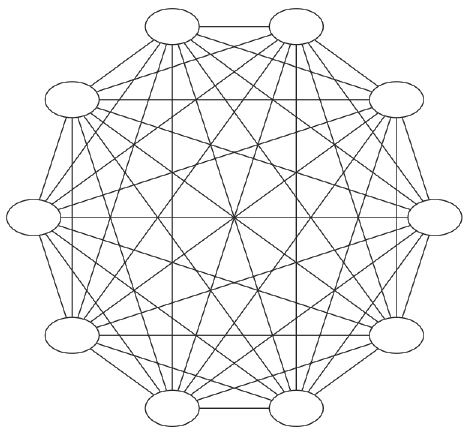
\includegraphics[width=0.8\textwidth]{Image001.jpg}
  \caption{电话网上有10个人通话的情况}
  \label{fig:phone10}
\end{figure}

\subsection{人工电话交换时代}

随着时代的发展，对电话有需求的用户越来越多，甚至普通家庭都希望拥有自己的电话。但是，为每对欲通话的家庭之间都铺设电话线是不可能的。因此，一种称为交换机（Switch，又称Exchange）的设备诞生了。它位于整个电话网的中心，用于连接每个用户。用户想打电话时，先拿起电话连接到管理交换机的接线员，由接线员负责接通到对方的线路。这便是最早的电话交换网（见图1-2），交换接续工作全部由人工完成。通过使用交换机，交换网上需要的线路大大减少了。

\begin{figure}[htbp]
  \centering
  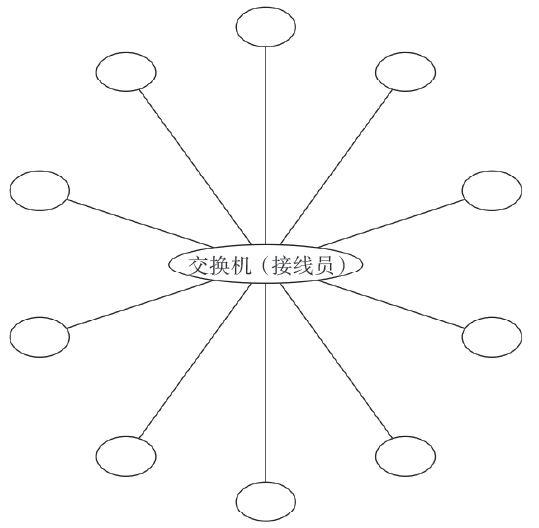
\includegraphics[width=0.8\textwidth]{Image002.jpg}
  \caption{人工电话交换网}
  \label{fig:manual_switch}
\end{figure}

\subsection{自动电话交换时代}

1889年到1891年期间，美国阿尔蒙·B·史端乔（Almon B Strowger）发明了步进式自动电话交换机。有趣的是，他发明自动交换机的目的并不是为了把接线员从繁忙的人工交换机上解放下来，而是来源于另外一则故事：他本是一个殡仪馆老板。他发觉每当城里发生死亡事件，用户给"殡仪馆"打电话时，不知接线员是有意还是无意的，总会把电话接到另一家殡仪馆。这使史端乔非常郁闷，发誓要将电话交换自动化。功夫不负有心人，史端乔凭他那过人的聪明和毅力，终于发明了一种步进式的自动电话交换机，并申请了专利。人们为了纪念他，故又称这种电话交换机为"史端乔交换机"（见图1-3）。这种交换机的特点是由用户话机的拨号脉冲直接控制交换机的动作，属于"直接控制"方式。

\begin{figure}[htbp]
  \centering
  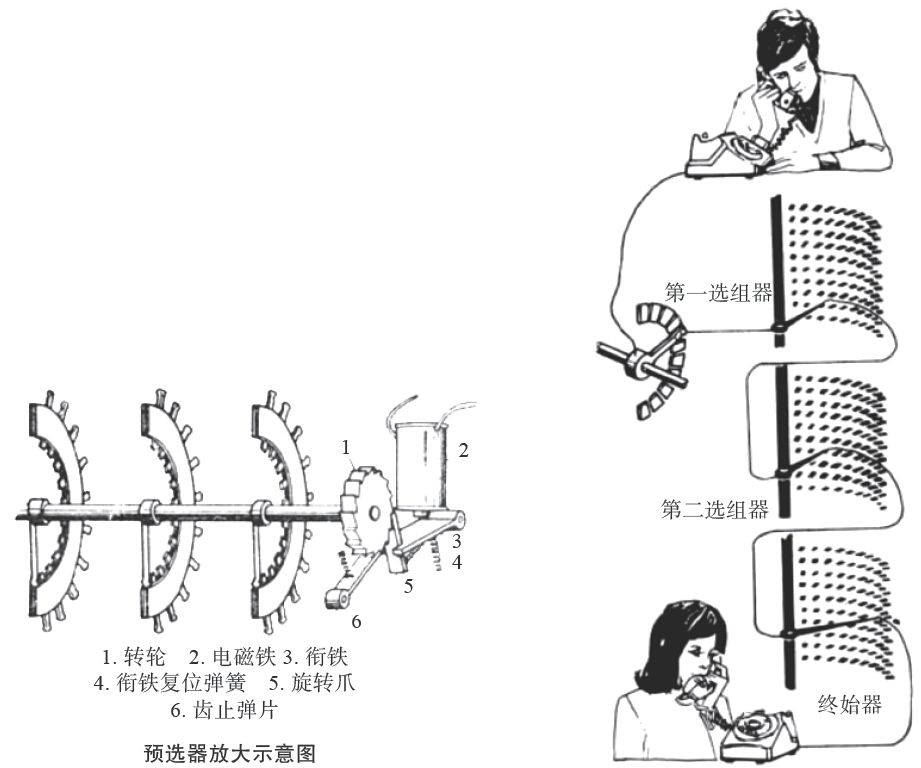
\includegraphics[width=0.9\textwidth]{Image003.jpg}
  \caption{步进式交换机4位拨号电话中继示意图}
  \label{fig:strowger}
\end{figure}

以后，又出现了旋转式（见图1-4）和升降式的交换机。这类交换机采用了一个称为"记发器"的部件来接收用户的拨号脉冲，然后将其通过译码器译成电码来控制接线器的动作，这属于"间接控制"方式。在采用记发器后，增加了选择的灵活性，从而使交换机的容量得到了提高。

\begin{figure}[htbp]
  \centering
  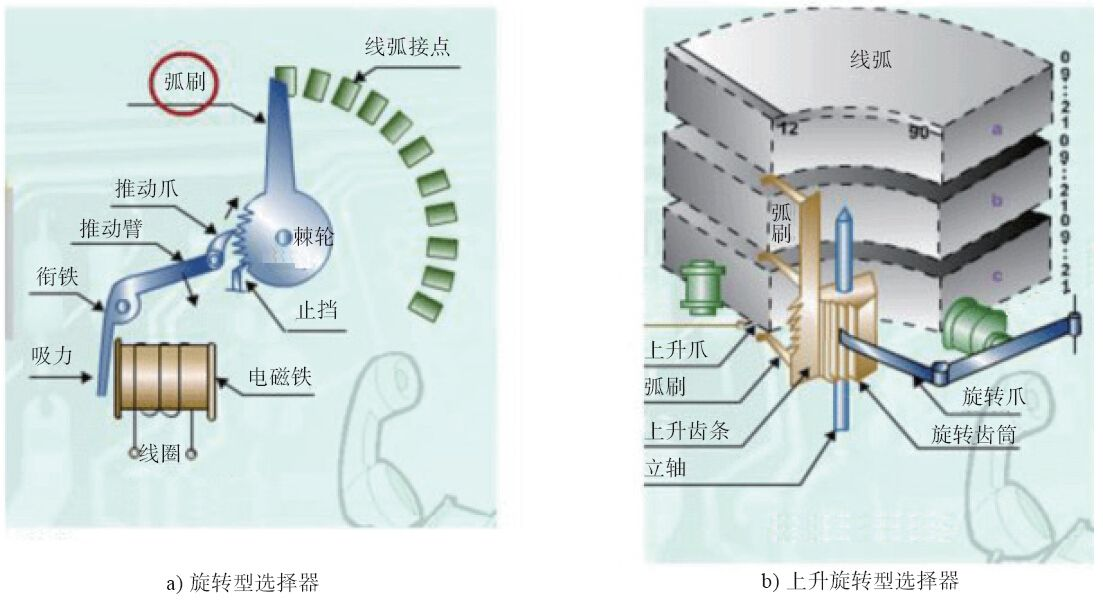
\includegraphics[width=0.9\textwidth]{Image004.jpg}
  \caption{旋转式交换机}
  \label{fig:rotary_switch}
\end{figure}

1919年，瑞典的电话工程师帕尔姆格伦和贝塔兰德发明了"纵横制接线器"（见图1-5），并申请专利。这种交换机将过去使用滑动摩擦方式的触点改成了压接触，减少了磨损，从而提高了交换机的寿命；而且，由于采用了导电性好的贵金属（如银）做金属触点，也大大提高了接触的可靠性。这种交换机的另一个特点是把控制部分和话路部分分开。控制部分由标志器和记发器来完成，称为公共控制。公共控制对用户拨号盘要求低，而中继部署的灵活性大大提高。

\begin{figure}[htbp]
  \centering
  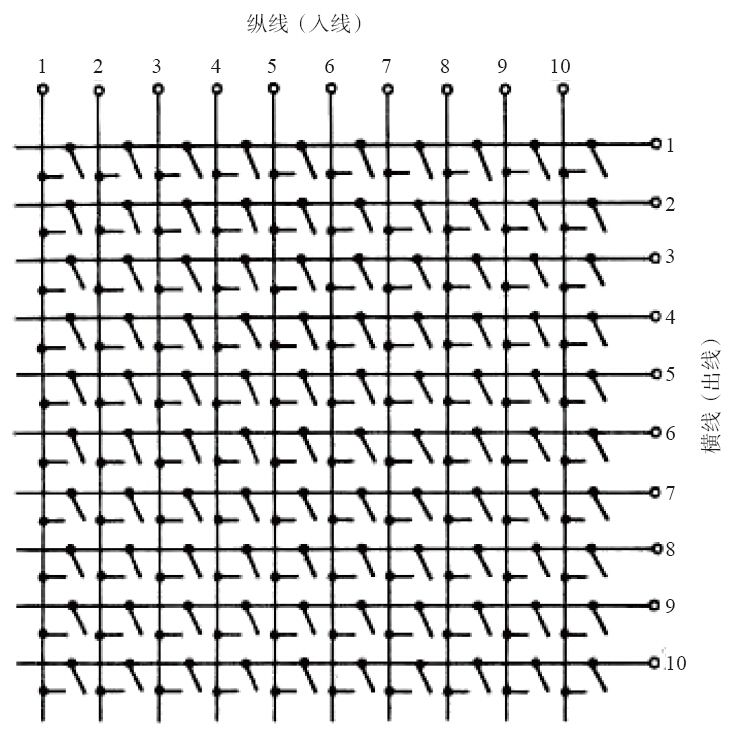
\includegraphics[width=0.7\textwidth]{Image005.jpg}
  \caption{纵横接线器交叉点示意图}
  \label{fig:crossbar}
\end{figure}

瑞典和美国分别在1926年和1938年开通了纵横制交换机，接着，法国、日本和英国也相继生产出纵横制交换机。

\subsection{半电子交换机时代}

随着电子技术，尤其是半导体技术的迅速发展，人们开始在交换机内引入电子技术，产生了电子交换机。由于当时技术条件的限制，仅在控制部分引入了电子技术，而话路部分在较长的一段时间内仍然采用机械触点。这种交换机一般称为半电子交换机或准电子交换机（区别是后者采用了速度较快的笛簧接线器）。

\subsection{空分交换机时代}

1946年，第一台由存储程序控制的电子计算机诞生，这对现代科学技术起到了划时代的作用。通过在交换机中引入"存储程序控制"的概念，1965年5月，美国贝尔系统的1号电子交换机（ESS No.1）问世了，这是世界上第一部开通使用的程控电话交换机。当时的交换机话路部分还保留了机械触点，以"空分"方式工作，因此称为空分交换机。并且，它交换的还是模拟信号。

\subsection{数字交换机时代}

20世纪60年代初以来，脉冲编码调制（PCM）技术成功地应用于传输系统中，它通过将"模拟"的信号数字化，提高了通话质量、增加了传输距离，同时，节约了许多线路成本。1970年，法国开通了世界上第一部程控数字交换机E10，开始了数字交换的新时代。

\subsection{现代PSTN时代}

随着技术的进步和人们对通信要求的增加，世界上许许多多的交换机间也需要相互通信，这些交换机之间通过中继线（Trunk）相连，随着电子交换机和程控交换机的发展，便出现了现代意义的PSTN网络。PSTN网络把世界上各个角落的人们都联系在了一起，很显然，有时一个通话需要穿越好多台交换机。

20世纪70年代后期出现了蜂窝式移动电话（当移动电话小到可以拿在手里的时候就开始叫"手机"了）系统，这是无线电话发展的里程碑。而在此之前，虽然无线电通信是在1895年发明的，但无线电话却是在20世纪初发明了真空三极管之后才出现的。1915年首次成功地实现了跨越大西洋的无线电话通信；1927年在美国和英国之间开通了商用无线电话。移动电话的出现，扩展了PSTN网络的能力和范围，对PSTN网络的影响极其深远。

专门用于移动电话交换的通信网络称为移动网，而原来的程控交换网则称为固定电话网，简称固网。简单来说，移动网就是在普通固网的基础上增加了许多基站（Base Station，可以简单理解为天线），并增加了归属位置寄存器（Home Location Register，HLR）和拜访位置寄存器（Visitor Location Register，VLR），以记录用户的位置（在哪个天线的覆盖范围内）、支持异地漫游等。移动交换中心称为MSC（Mobile Switch Center）。

\subsection{下一代网络及VoIP时代}

随着分组交换技术的成熟及因特网的发展，人们认识到了将原始的基于电路交换的语音网络与基于分组交换的因特网络进行融合（即语音通信和数据通信相结合）的必要性，因此一个称为NGN（Next Generation Network）的概念被提了出来。NGN是指下一代网络，ETSI\footnote{European Telecommunications Standards Institute，即欧洲电信标准化协会，官方网站是http://www.etsi.org。}对它的定义是："NGN是一种规范和部署网络的概念，即通过采用分层、分布和开放业务接口的方式，为业务提供者和运营者提供一种能够逐步演进的策略，实现一个具有快速生成、提供、部署和管理新业务的平台。"\footnote{原文是：NGN is a concept for defining and deploying networks,which,due to their formal separation into different layers and planes and use of open interfaces,offers service providers and operators a platform which can evolve in a step-by-step mannerto create,deploy and manage innovative services.不过，这个概念的定义跟它的名字一样令人迷惑。事实上，这个概念最早大约是在1997年提出来的，所以，"下一代"中的"下"早就过时了。}

在NGN提出之后，经过数年的研究和探索，人们提出了各种NGN的解决方案，但最终基本上都统一到了IMS（IP Multimedia Subsystem）技术\footnote{一般来说，NGN就应该称为软交换，而有的人也说IMS是更软的软交换。读者到后面就能了解到，与"更软的软交换"相比，FreeSWITCH更是用纯软件实现的，或许可以称做是"更更软的软交换"了。当然软交换的"软"并不是取决于它是否用"软件"来实现，而是更强调基于分组网的交换网络中的呼叫控制功能与媒体网关的分离。}。IMS运行于标准的IP网络上，使用一种基于第三方伙伴计划（3GPP）的SIP标准的VoIP实现方式。IMS的目标不仅是在现有网络基础上提供新的业务，它还要能提供在未来的因特网上能够承载的所有的业务。

当然，IMS属于核心交换层的技术，它全部基于IP网络，但在接入层，目前的语音大部分还是基于电路接入的方式接入的，因此，这就要求在一定时间内IMS在接入层要继续兼容电路接入。同时，在无线移动通信领域，随着移动通信技术的成熟及众多智能终端的出现，对高速IP网络的要求也就越来越迫切。最新的3G\footnote{3G是指第三代移动通信技术，与第一代（1G、模拟系统）和第二代（2G、以GSM为代表的数字系统）移动通信技术相比，它主要是支持高速IP数据传输。详见http://zh.wikipedia.org/wiki/3G。}、4G\footnote{4G是指第四代移动通信技术，是3G之后的延伸，从技术标准的角度看，按照ITU的定义，静态传输速率达到1Gbps，用户在高速移动状态下可以达到100Mbps，就可以称为4G的技术。详见http://zh.wikipedia.org/wiki/4G。}技术就是应此要求而产生的。未来的通信中要完全取消低效的电路传输及电路交换，而全部集中到IP通信上来，也就催生了一个新的无线通信标准LTE\footnote{参见http://zh.wikipedia.org/wiki/长期演进技术。}。LTE的定义是长期演进而来的，其为现代的手机及其他移动设备提供了高速的数据通信手段，逐步实现了全IP交换。

关于通信网络的演进，简单来说，在无线方面体现为从GSM/CDMA/UMTS等向LTE发展，在核心网方面则体现为从电路交换向IMS发展。过去几年，围绕LTE语音曾经出现过多种观点、技术和演进路线。由于LTE标准不再支持用于支撑GSM、UMTS和CDMA2000网络下语音传输的电路交换技术，它只能进行全IP网络下的分组交换，因此随着LTE网络的部署，运营商需选择VoLTE\footnote{VoLTE（Voice Over LTE，LTE网络直传）：该方案基于IP多媒体子系统（IMS）网络，配合GSMA在PRD IR.92中制定的LTE控制和媒体层面的语音服务标准。使用该方案意味着语音将以数据流形式在LTE网络中传输，所以无须调用传统电路交换网络，旧网络无须保留。简单来说，VoLTE就是LTE网络环境下的VoIP业务。}、CSFB\footnote{CSFB（Circuit Switched Fallback，电路交换网络支援）：该方案中的LTE网络将只用于数据传输，当有语音拨叫或呼入时，终端将使用原有电路交换网络。该方案只需运营商升级现有MSC核心网而无须建立IMS网，因此运营商可以较迅速地向市场推出网络服务。也由于语音通话需要切换网络才能使用的缘故，通话接续时间将被延长。}、SVLTE\footnote{SVLTE（Simultaneous Voice and LTE，LTE与语音网同步支持）：该方案使用可以同时支持LTE网络和电路交换网络的终端，使得运营商无须对当前网络作太多修改。但这同时意味着终端价格的昂贵和电力消耗的迅速。}、OTT\footnote{OTT（Over-The-Top）：一种将服务建于网络之上的方式，如用Skype来提供LTE的语音。LTE具备高带宽、低时延、永远在线、全IP等特点，为OTT的发展带来了天然的便利，使得OTT语音几乎没有壁垒。但应当看到，现在乃至将来很长时间里，语音业务都是移动运营商的最主要的收入来源，把LTE的语音业务完全交给OTT是一种非常激进的观点，在电信领域得到的支持并不多。}等方法之一解决LTE网络中的语音传输问题。从目前来看，移动网络庞大且复杂，在网络建设初期大部分运营商都选择使用CSFB方式建设网络，这种方式便于快速部署系统。当然，CSFB只是过渡时期的临时解决方案。从长远来看，VoLTE及其他几种方案更符合未来网络的发展方向。据报道，中国移动已于2013年6月发布了VoLTE技术白皮书，并计划于2014年下半年展开大规模商用。未来通信网络将走向何方，让我们拭目以待。

\section{电话实现技术}

电话系统的发展与科技的进步是分不开的。在本节，我们来介绍一些关键的电话技术及专业术语。

\subsection{电话号码}

我们的生活已经离不开电话，而要打电话就离不开电话号码。但好多人对天天使用的电话号码既熟悉又陌生，因此，在这里我们也补充一些现行的电话网中电话号码的知识。值得注意的是，这些号码的出现大部分与业务内容和行政区划有关，也有一些历史背景，但限于篇幅，我们就不深入讨论了。

\subsubsection{固定电话号码}

现行的电话网中采用E.164\footnote{参见http://en.wikipedia.org/wiki/E.164。}号码格式。以我国固话电话的编号规则为例，我们先来看本地号码。

一般来说，在比较大的省市（如北京、上海等）使用8位号码，比较小的省市使用7位号码。以北京的电话号码为例，它由8位数字组成，表示为ABCD EFGH，其中，ABCDE称为一个千群，即该群可以包含1000个电话号码，同理ABCD称为一个万群。小规模的交换机可能只包含几个千群，而大规模的可能包含几个万群。

如果在不同的省市之间打电话，则称为长途电话，一般需要通过长途局进行路由。打长途电话需要在本地号码前加上长途区号。根据城市的大小不同，我国电话区号的长度一般是2位到3位，如：

\begin{verbatim}
10   北京
20   广州
21   上海
755  深圳
535  烟台
\end{verbatim}

读者可能会问，北京的长途区号不是010吗？答案是——"不是！"许多人会错误地认为北京的区号是010，这也正是作者要写这一节的原因。

由于各地区号的长度不同，而且数字也不规则，因此，为了区分长途电话和本地电话，我国规定，在拨打长途电话前除了要加上区号外，还要在最前面加"0"。因此，"0"是国内长途字冠，它本身不是区号的一部分。为了帮助读者理解，我们先考虑国际长途的情况。为了区分国内长途与国际长途，我国规定，国际长途要在国家代码前加两个0。因此，如果拨打美国的号码，如：1-234-567-890，则需要拨00-1-234-567-890。其中，1为美国的国家代码，我们稍后还会讲到。

交换机的拨号规则遵循短号优先的原则，拨号时不加0就认为是本地号码，加一个0就认为是国内长途，两个0是国际长途。我国的国家代码是86，因此，一个北京号码的国际表示是：86 10 ABCD EFGH。

与我国不同，美国的国际长途字冠是011，因此如果从美国拨打中国的号码，则需要拨：011 86 10 ABCD EFGH。

类似的，其他国家和地区也有不同的拨号方式，这增加了电话号码书写的复杂性。因此，在实际书写电话号码时，有时会省略国际长途字冠，而统一用"+"号代替，如：+86 10 ABCD EFGH\footnote{当然，为了方便阅读，有时还会在电话电码中增加括号和短横线。}。

读到这里，读者就可以理解为什么北京的区号不是010了吧？另外，我们还知道，使用固定电话拨打异地手机时前边要加拨0，同样说明0并不是区号或手机号码的一部分。

\subsubsection{移动电话号码和专用号段}

移动电话号码俗称手机号，由于其可移动与漫游的特性，因此与普通固定电话号码略有不同。众所周知，我国的移动电话号码都是以1开头的，按不同的运营商来划分。如中国移动的号码由135、136、137、138、139等开头；中国联通的由130、186等开头，中国电信的由133、189等开头。它们后面都是8位的号码，因此整个手机号共11位，前3位称为移动电信运营商专用的号段。

在2013年工信部发放虚拟运营商牌照以后，核发170号段作为虚拟运营商的专用号段。

\subsubsection{短号码}

有一类特殊的号码称为短号码，如大家熟知的110、119、120等，这些属于公益性的号码（又称紧急号码，供紧急情况下使用），拨打都是免费的。

还有一部分是预付费的电话卡类业务，如200、201、300等。拨打这类号码本身不收费，而从关联的电话卡上扣费。

另一些短号码，如114等，由于运营商的分拆、合并，有的演变成了116114；还有一些5位的短号码专门供一些大的集团（如银行等）使用，如95555、95588等，这些号码不论何时何地拨打，一般只收市话费。

这些短号码的资源比较紧张，一般不会给个人使用。另外还有其他一些短号码，我们就不多讲了。

\subsubsection{800和400号码}

%800开头的号码是被叫付费的业务，主叫呼叫这些号码是免费的。这些号码主要由一些大的企业集团使用。这类号码都是虚拟的电话号码，在实际呼叫过程中通过查%询数据库转换成真正的目的号码。
%
%但是800号码有一个致命的缺点，就是用手机打不通，这主要是电信业务的历史原因（主要原因是不同运营商的网间结算）造成的。随着移动业务的发展，手机用户%越来越多，因此，出现了400业务。这类业务的特点是主被叫分摊付费，主叫付本地通话费，被叫付长途电话费（如果主被叫不在一个城市）。400业务是手机用户可%以呼叫的。
%
%当然，随着时代的发展，以及各运营商提供更加灵活的话务套餐（如主叫免收长途费等），主叫用户对拨打这类号码时对实际资费已不太敏感。拥有800和400之类的%电话号码越来越多地成为了企业实力和社会形象的标志。
%
%\subsubsection{北美电话号码分类计划}
%
%为了与国内号码进行对比，我们来简单说一下北美电话号码分类计划（North American Numbering Plan\footnote{参见http://zh.wikipedia.org/wiki/北%美电话号码分类计划。}）。
%
%加拿大和美国使用北美电话号码分类计划，其区号由3位数字组成，本地号码为7位数字，1为长途接入码，即长途字冠（在有的情况下可以省略长途字冠）。比如，%一个完整的号码为1（ABC)DEF-GHIJ，如果是在本地拨打，则可以直接拨"DEF GHIJ"，如果是拨打长途，则需要先拨长途字冠1及区号，即：1（ABC)DEF-GHIJ。
%
%值得一提的是，其中的区号ABC如果是555，除555-1212是查号台外，其他的号码都是不存在的。这类号码一般用于电影或戏剧中，防止与真实环境中的电话号码相%冲突。
%
%\subsubsection{电话号码的书写格式}
%
%电话号码就是一长串号码，但有时候为了便于阅读，在写的时候常用连字符"-"、括号、空格等将数字分开，如上一节我们看到美国电话号码的格式。
%
%国内电话号码的书写一般采用如下的方式：
%
%\begin{verbatim}
%（010) ABCD EFGH    （没有国家代码，虽然0不是区号的一部分，但是，习惯了）
%+86 （10) ABCD EFGH  （固话，8位，国际号码格式）
%+86 （535) ABC DEFG  （固话，7位，国际号码格式）
%+86 139 ABCD EFGH   （手机，国际号码格式）
%\end{verbatim}
%
%当然，具体的写法没有统一的规定，只要让看到号码的人知道怎么拨打就行了。至于要将电话号码印到名片上，又涉及企业形象设计的问题了，那就另当别论了。
%
%\subsection{模拟信号与数字信号}
%
%模拟（Analog）量是连续的变化的量，如温度、声音等。早期的电话网也是基于模拟交换的。对于人类交流来讲模拟信号是非常理想，但它很容易引入噪声。如果通%话双方距离很远，信号会衰减，因而需要对信号进行放大。问题是，信号中经常混入线路的噪声，放大信号的同时也放大了噪声，导致信噪比（信号量与噪声的比%例）下降，严重时甚至会难以分辨。
%
%数字（Digital）信号是不连续的（离散的），是按一定的时间间隔（单位时间内抽样的次数称为频率）对模拟信号进行抽样（见图1-6）得出的一些离散值。然后%通过量化和编码过程就可将这些离散值变成数字信号。根据抽样定理\footnote{又称采样定理或奈奎斯特·香农定理，见http://zh.wikipedia.org/wiki/采样定%理。}，当抽样频率是模拟信号最高频率的2倍时，就能够完全还原原来的模拟信号。
%
%\begin{figure}[htbp]
%  \centering
%  
\includegraphics[width=0.9\textwidth]{Image00053.jpg}
%  \caption{抽样}
%  \label{fig:sampling}
%\end{figure}
%
%\subsection{PCM}
%
%PCM（Pulse Code Modulation）的全称是脉冲编码调制。它是一种通用的将模拟信号转换成以0和1表示的数字信号的方法。
%
%一般来说，人的声音频率范围在300~3400Hz之间，通过滤波器将超过4000Hz的频率过滤出去，便得到4000Hz内的模拟信号。然后根据抽样定理，使用8000Hz进行%抽样，便得到离散的数字信号。使用PCM方法得到的数字信号就称为PCM信号，一般一次抽样会得到16bit的信息。
%
%为了更有效地在线路上进行传输，通常对PCM信号进行一定的压缩。通过使用压缩算法\footnote{实际为压扩法，因为有的部分是压缩的，有的是扩张的。目的是给%小信号更多的比特位数以提高语音质量。}，可以将每一个抽样值压缩到8bit。这样1秒的抽样就得到8bit×8000=64000bit的信号（简称64kbit），抽样速率（即%传输速率）为64kbit/s\footnote{bit/s即比特/秒，有时也写作bps（Bit Per Second）。注意，通常，对于二进制数来说K为大写，1K=1024，但此处的k为小%写，1k=1000。}。
%
%PCM通常有两种压缩方式：A律和μ律。其中北美使用μ律，我国和欧洲使用A律。这两种压缩方法很相似，都采用8bit的编码获得12bit到13bit的语音质量%\footnote{目前我国使用的是A律13折线特性。基本原理是：使用非均匀量化方法和压缩扩张技术得到13段折线。感兴趣的读者可在Google上搜索"13段折线"进行%更深入的了解。}。但在低信噪比的情况下，μ律比A律略好。A律也用于国际通信，因此，凡是涉及A律和μ律转换的情况，都由使用μ律的国家负责。
%
%\subsection{局间中继与电路复用技术}
%
%连接交换机（局）的E1或T1电路称为局间中继。交换机间的消息以及通话数据都是在局间中继上传送的，传统的交换机使用时分复用（TDM）技术将多路通话合并到%一条数字中继线上，可以大大节省局间中继线的数量。
%
%利用时分复用技术可以将32个64kbit/s的信道合并到一条2Mbit/s（64kbit/s×32=2.048Mbit/s，通俗来说就直接叫一个两兆）的电路上，这样的电路称为一个E1%（在北美和日本，是24个64kbit/s复用，称为T1，速率是1.544Mbit/s）。在E1中，每一个信道称为一个时隙。其中，除0时隙固定传同步时钟外，其他31个时隙%最多可以同时支持31路电话（有时候会使用第16时隙传送信令，这时最多支持30路电话）。
%
%随着话务量的增加，交换机之间的电路越开越多，因而需要更高级别的电路复用技术。目前通常的做法是将63个E1合并到一个155Mbit/s（2×63+P=155，其中P是电%路复用的开销）速率的光路（光纤）上，在SDH（Synchronous Digital Hierarchy，同步数字传输体系）技术中这称为STM-1（Synchronous Transfer %Module，同步传输模块）。
%
%当然，155Mbit/s速率的光路还可以使用波分复用等技术合并到1Gbit/s或10Gbit/s速率的光路上，实现话路收敛和传输。
%
%\section{我国电话网结构}
%
%我国的电话网由本地网与长途网组成，并通过国际交换中心进入国际电话网。
%
%原有电话网的结构采用了等级制，共有五级，分别用C1～C5表示。其中C1～C4构成长途电话网，C5（端局）及汇接局（Tm）构成本地网。但随着社会和经济的发%展，电话业务量迅速增加，横向话务流量日趋增多，新业务的需求不断涌现，五级网络结构由于转接段数多造成了接续时延长、传输损耗大、网络管理工作复杂、不%利于新业务的开展等问题。因此，我国电话网正在由五级电话网向三级电话网转变，即将原来的C1级和C2级长途交换中心演变为DC1，原来的C3级和C4级交换中心演%变为DC2，以便减少转接段数。下面，我们主要以本地网为例简单讲解一下电话网的结构。
%
%图1-7所示的主体部分为我国一地级市固定电话网（称为本地网）的结构。通常，用户话机（如A、B、C、D）通过一对电话线连接到距离最近的交换机上，该交换机%称为端局交换机（一般以区或县为单位）。端局交换机通过局间中继线连接到汇接局\footnote{为了保证安全，汇接局通常会成对出现，平常实行负荷分担，一台%汇接局出现故障，与之配对的汇接局会承担其负责的所有话务。}。长途电话需要通过所在长途局与其他长途局相连。但根据话务量要求，汇接局也可以直接与其他%长途局开通高速直达中继（未画出）。为节省用户线，在一些人口比较集中的地方（如学校、小区），会在端局下再设模块局或接入网，用户话机（如a、b、c、d、%e）则就近接入到模块局（或接入网）上。
%
%\begin{figure}[htbp]
%  \centering
%  
\includegraphics[width=0.8\textwidth]{Image00135.jpg}
%  \caption{我国固定电话网结构}
%  \label{fig:china_phone_network}
%\end{figure}
%
%在我国，智能网一般用于实现电话卡、预付费或400/800类业务，而前几年新部署的NGN（Next Generation Network，下一代网络，一般指软交换）则支持更灵%活、更复杂的业务，包括IM/SMS/MMS等消息类业务、点对点交互式多媒体/文件共享/游戏等多方协作交互业务、内容分发业务、广播/多播业务、企业托管业务，以%及数据检索、数据通信、在线应用、传感器网络、远程控制等各类多媒体业务和数据业务。
%
%但是技术发展很快，为响应国家"光进铜退"\footnote{用户家里的电话线使用铜双绞线。}的号召，现在已经实现了直接光纤到户，也就是说很快全网都能IP化了。%新技术代替旧技术，为用户带来了五彩斑斓的业务，但旧技术的一些优点则永远让人怀念，最典型的就是原来的电话线是带电的，家里停电不影响打电话。但光纤是%不带电的，停电以后用户就不能打电话了（除非加UPS）。
%
%在我国的移动网络中，大量部署了IMS。IMS具有组网灵活的优点，但涉及的网元和基本概念很多，对于非专业人士来说理解起来有些困难。我们将在本章的最后一节%对IMS进行专门的讨论。
%
%\section{信令}
%
%用户设备（如话机）与端局交换机之间，以及交换机与交换机之间需要进行通信。这些通信所包含的信息有（但不限于）用户、中继线状态、主叫号码、被叫号码、%中继路由的选择等。我们把这些消息称为信令（Signaling）。
%
%\subsection{信令分类}
%
%按照不同分类方式，信令可以分成很多种。下面介绍信令主要的几种分类方式。
%
%（1）按信令的功能分
%
%按照功能的不同，信令可以分成以下三种：
%
%\begin{itemize}
%  \item 线路信令：具有监视功能，用来监视主被叫的摘、挂机状态及设备忙闲。
%  \item 路由信令：具有选择功能，指主叫所拨的被叫号码，用来选择路由。
%  \item 管理信令：具有操作功能，用于电话网的管理和维护。
%\end{itemize}
%
%（2）按信令的工作区域分
%
%信令按照工作区域的不同可以分成以下两种：
%
%\begin{itemize}
%  \item 用户线信令：是用户终端与交换机之间的信令。它包括用户状态（摘、挂机）信号、用户拨号（脉冲、DTMF）所产生的数字信号，以及交换机向用户终端%发送的信号（铃流、信号音）。
%  \item 局间信令：是交换机和交换机之间的信令，在局间中继线上传送，用来控制呼叫接续和拆线。
%\end{itemize}
%
%\textbf{注意}：用户线信令少而简单，局间信令多而复杂。
%
%（3）按信令的信道分
%
%按照信道的不同，信令可以分为以下两种：
%
%\begin{itemize}
%  \item 随路信令：信令和话音在同一条话路中传送。
%  \item 公共信道信令：以时分方式在一条高速数据链路上传送一群话路。
%\end{itemize}
%
%随路信令传送速度慢，信息容量有限（传递与呼叫无关的信令能力有限）；公共信道信令传送速度快、容量大，具有改变或增加信令的灵活性，便于开放新业务。
%
%（4）其他分类
%
%另外，信令还可分为带内信令和带外信令、模拟信令和数字信令、前向信令和后向信令、线路信令和记发器信令等，我们在这里就不多解释了，有兴趣的读者可以自%行搜索相关的关键词进一步学习。
%
%下面我们分别对一些重要的信令进行简单介绍。
%
%\subsection{用户线信令}
%
%从用户终端（通常是话机）到端局交换机之间经常需要传送一些控制信息，如用户摘机、挂机、拨号、主叫号码显示等，这些信息称为用户线信令。用户线信令可以%通过模拟或数字信号传递。
%
%对于普通的话机，线路上传送的是模拟信号，因此信令只能在电话线路上传送，这种信令称为带内信令。话机通过电压变化来传递摘、挂机信号；通过DTMF（Dual %Tone Multi Frequency，双音多频\footnote{话机上每个数字或字母都可以发送一个低频和一个高频信号相结合的正弦波，交换机经过解码即可知道对应的话机%按键。}）传送要拨叫的电话号码。另外，也可以通过移频键控（Frequency Shift-keying，FSK）技术来支持主叫号码显示，俗称来电显示（Caller Line %Identification Presentation，Caller ID或CLIP，主叫线路识别提示）。
%
%与普通电话不同，ISDN（Integrated Service Digital Network，综合业务数字网）在用户线上传送的是数字信号。它的基本速率接口（Base Rate %Interface，BRI）使用144kbit/s的2B+D信道——两个64kbit/s的B信道及一个16kbit/s的D信道。其中B信道一般用来传输话音、数据和图像，D信道用来传输信令%或分组信息。
%
%2B+D的ISDN最初是为了解决用户线上的语音与数据同步传输问题。但事实上，2B+D的ISDN并不像传说中那么美，而且需要专门的NT1终端设备，在我国并没有发挥%出它应有的作用，后来很快被ADSL技术取代了。
%
%\subsection{局间信令}
%
%交换机与交换机之间也需要传送控制信号，用于话路的建立、释放等，这些控制信号就称为局间信令。局间信令主要在局间中继上传送，传送局间信令的电路称为信%令链路。一般来说，一条信令链路通常只占用一个64kbit/s的时隙。一条信令消息通常只有几十或上百个字节，一条64kbit/s的电路足以容纳成千上万路电话所需%要的信令。但随着技术的进步、话务量的上涨以及更多增值业务的出现，完成一次通话需要更多的信令消息，因此出现了2Mbit/s速率的信令链路，即整个E1链路上%全部传送信令。
%
%目前在传统的PSTN网络中常见的局间信令有ISDN PRI（Primary Rate Interface，基群速率接口）信令和七号信令。PRI信令和话路在同一个E1上传送，通常使%用第16时隙，而0时隙传送同步信号，其他30个时隙可传输通话信息，因此又称30B+D。与PRI信令不同，七号信令除可以与话路在同一个E1上传送外，还可以在专门%的用于传送信令链路的E1中继上传送，因而它组网更加灵活，支持更大的话务量。我们将在下一节专门讲解七号信令。
%
%支持七号信令的每个通信设备都需要有一个全局唯一信令点编码，而信令点编码资源是比较有限的。因而，七号信令主要在运营商的设备上使用，而运行商与用户设%备（如PBX）一般使用PRI信令对接。
%
%\subsection{七号信令}
%
%七号信令（Signaling System No.7，SS7）是我国目前使用的主要信令方式，用于局间通信。我国的电话网络中有专门的七号信令网。
%
%在此，我们先来看一次简单的固定电话的通话流程。如图1-8所示，用户a摘机，与其相连的交换机A根据电压、电流的变化检测到a摘机后，即向a发送拨号音，同时%启动收号程序。a听到拨号音后开始拨号，待交换机A收齐号码后，即查找路由，发送IAM（Initial Address Message，初始地址消息）给交换机B。B向A发ACM%（Adress Complete Message，地址全消息）并通知用户b（b的话机）振铃，A向a送回铃音。这时如果b接听电话，则B向A发送ANC（Answer Charge，应答计费%消息），a与b开始通话，同时A对a进行计费\footnote{B也可以对A计费，这种收费方式称为中继计费，主要用于局间结算（话费）。如果A和B分属于不同的运营商%（如移动和电信），则称为网间结算。}。
%
%\begin{figure}[htbp]
%  \centering
%  
\includegraphics[width=0.8\textwidth]{Image00137.jpg}
%  \caption{七号信令局间呼叫流程}
%  \label{fig:ss7_call_flow}
%\end{figure}
%
%通话完毕，如果主叫挂机，则本端交换机A向对端B发送CLF（Clear Forward，前向释放消息），B向A返回RLG（ReleaseGard，释放监护消息），并向b传送催挂%音（嘟嘟嘟……）。
%
%如果被叫挂机，则B向A发送CBK（Clear Backword，后向释放消息），A回送CLF，最后B返回RLG。
%
%上面在交换机A与B之间传递的为七号信令中的TUP（Telephone User Part，电话用户部分）。目前，由于ISUP（ISDN User Part，ISDN用户部分）能与ISDN互%联并提供比TUP更多的能力和服务，故其已基本取代TUP成为我国七号信令网采用的主要信令方式。ISUP信令与TUP互通时的对应关系如图1-9所示。
%
%\begin{figure}[htbp]
%  \centering
%  
\includegraphics[width=0.8\textwidth]{Image00048.jpg}
%  \caption{ISUP与TUP互通信令流程}
%  \label{fig:isup_tup}
%\end{figure}
%
%图1-9所示为端局A与端局B经过汇接局TM汇接通信中ISUP与TUP信令的例子。ISUP信令的初始地址消息有IAM和IAI（IAM With Additional Information，带附%加信息的IAM）两种，后者能提供更多的信息（如主叫号码等）。另外ISUP信令的拆线信号不分前后向，只有REL（Release，释放）和RLC（Release Complete，%释放完成）。
%
%在上一节中我们提到了ISDN PRI信令，出于完整性的考虑，这里我们也来看一下ISUP与ISDN PRI信令互通的例子。ISDN PRI使用SETUP/CONNECT/RELEASE消息分%别对应ISUP中的IAM/ANM/REL消息，如图1-10所示。
%
%\begin{figure}[htbp]
%  \centering
%  
\includegraphics[width=0.85\textwidth]{Image00049.jpg}
%  \caption{ISUP与ISDN互通的信令流程}
%  \label{fig:isup_isdn}
%\end{figure}
%
%\subsection{H.323与SIP信令}
%
%H.323与SIP属于VoIP领域的通信信令，它们适用于用户线信令和局间信令，由于IP终端比普通话机更加智能，因此这些信令在用户线信令及局间信令使用方式上已%没有太大区别。
%
%H.323是ITU多媒体通信系列标准H.32x的一部分，该系列标准使得在现有通信网络上进行视频会议成为可能，其中，H.320是在N-ISDN上进行多媒体通信的标准；%H.321是在B-ISDN上进行多媒体通信的标准；H.322是在有服务质量保证的LAN上进行多媒体通信的标准；H.324是在GSTN和无线网络上进行多媒体通信的标准。H.%323为现有的分组网络PBN（如IP网络）提供多媒体通信标准，若和其他的IP技术（如IETF的资源预留协议RSVP）相结合，就可以实现IP网络的多媒体通信。
%
%SIP（Session Initiation Protocol，会话发起协议）是由IETF（Interne工程任务组）提出的IP电话信令协议。正像其名字所隐含的那样，SIP用于发起会%话，它能控制多个参与者参加的多媒体会话的建立和终结，并能动态调整和修改会话属性，如会话带宽要求、传输的媒体类型（语音、视频和数据等）、媒体的编解%码格式、对组播和单播的支持等。
%
%H.323和SIP设计之初都是作为多媒体通信的应用层控制（信令）协议，目前一般用于IP电话。它们能实现的信令功能基本相同，也都利用RTP作为媒体传输的协议。%但两者的设计风格截然不同，这是由于推出它们的两大阵营（电信领域与Internet领域）都想沿袭自己的传统。H.323是由国际电信联盟提出来的，它企图把IP电话%当作众所周知的传统电话，只是传输方式由电路交换变成了分组交换，就如同模拟传输变成数字传输、同轴电缆传输变成了光纤传输。而SIP侧重于将IP电话作为%Internet上的一个应用，较其他应用（如FTP，E-mail等）增加了信令和QoS的要求。H.323推出较早，协议发展得比较成熟，由于其采用的是传统的实现电话信令%的模式，故便于与现有的电话网互通，但相对复杂。SIP借鉴了其他Internet标准和协议的设计思想，有其突出的优点。
%
%\begin{itemize}
%  \item SIP是基于文本的协议，而H.323采用基于ASN.1和压缩编码规则的二进制方法表示其消息，因此，SIP对以文本形式表示的消息的词法和语法分析比较简%单。
%  \item SIP会话请求过程和媒体协商过程等是一起进行的，因此呼叫建立时间短，而在H.323中呼叫建立过程和进行媒体参数等协商的信令控制过程是分开进行%的。
%  \item H.323为实现补充业务定义了专门的协议，如H.450.1、H.450.2和H.450.3等，而SIP只要充分利用已定义的头域，必要时对头域进行简单扩展就能很方%便地支持补充业务或智能业务。
%  \item H.323进行集中、层次式控制。尽管集中控制便于管理（如便于计费和带宽管理等），但是当用于控制大型会议电话时，H.323中执行会议控制功能的多点%控制单元很可能成为瓶颈。而SIP类似于其他的Internet协议，设计上为分布式的呼叫模型服务，具有分布式的组播功能。
%\end{itemize}
%
%关于SIP信令我们将在第8章详细讲解，读者可以先在这里参考一下图1-11所示的ISUP与SIP间的信令转换关系图，以便建立一个直观的印象。
%
%\begin{figure}[htbp]
%  \centering
%  
\includegraphics[width=0.8\textwidth]{Image00139.jpg}
%  \caption{ISUP与SIP互通的信令流程}
%  \label{fig:isup_sip}
%\end{figure}
%
%\section{媒体}
%
%信令主要传输一些控制信号，而通信双方需要听到的是对方的语音数据，这些语音数据就称为媒体（Media）。随着通信系统能力的提高及更加高级、智能的终端设%备的出现，通信系统所能传输的媒体类型也越来越丰富，比较典型的有我们刚才提到的语音，还有视频、文字信息（短消息）、传真等。
%
%在SIP通信中，除文字外，媒体都是在RTP协议中传输的。由于媒体一般都是持续传输的，因此又称RTP流。
%
%举一个通俗一点例子：假设张三乘火车从北京到南京，那么张三就是媒体。而火车称为承载（或载体，Carrier）。为了保证正常运行，火车需要听从控制信号的指%挥，而这些控制信号就相当于信令。如果信令出了问题，媒体就可能无法正常到达了。当然这个比方可能不十分恰当，你也可以认为张三和火车都是媒体，只不过张%三被火车"包"了一层，而铁路才是真正的载体。不管怎么说，在SIP通信中，SIP相当于这里的火车控制信号，RTP流中的语音数据相当于很多张三，他们被RTP又"包%"了一层，通过以太网承载到达目的地。
%
%\section{电路交换与分组交换}
%
%在传统的电路交换中，两个通信节点间需要建立一个专用通路，这会导致电路利用率较低。而报文交换以报文作为数据交换的单位，携带目标地址、源地址等信息，%在节点间采用存储转发的方式，不需要建立专门的通信线路，可以大大提高通信线路的利用率。分组交换是报文交换的特殊情形，下面我们来介绍一下电路交换和分%组交换\footnote{参考自：http://baike.baidu.com/view/188266.htm。}。
%
%\subsection{电路交换}
%
%传统的电话都是基于电路交换的。由于电路交换在通信之前要在通信双方之间建立一条被双方独占的物理通路（由通信双方之间的交换设备和链路逐段连接而成），%因而有以下优缺点。
%
%电路交换的优点：
%
%\begin{itemize}
%  \item 由于通信线路为通信双方用户专用，数据直达，所以传输数据的时延非常小。
%  \item 通信双方之间的物理通路一旦建立，双方可以随时通信，实时性强。
%  \item 双方通信时按发送顺序传送数据，不存在失序问题。
%  \item 电路交换既适用于传输模拟信号，又适用于传输数字信号。
%  \item 进电路交换的设备（交换机等）及控制均较简单。
%\end{itemize}
%
%电路交换的缺点：
%
%\begin{itemize}
%  \item 电路交换的平均连接建立时间对计算机通信来说较长。
%  \item 建立电路交换连接后，物理通路被通信双方独占，即使通信线路空闲，也不能供其他用户使用，因而信道利用率低。
%  \item 在进行电路交换时，数据直达，不同类型、不同规格、不同速率的终端很难相互进行通信，也难以在通信过程中进行差错控制。
%\end{itemize}
%
%\subsection{分组交换}
%
%我们熟悉的IP交换采用的就是分组交换的方式。它仍采用存储转发的传输方式，但将一个长报文先分割为若干个较短的分组，然后把这些分组（携带源、目的地址和%编号信息）逐个地发送出去，因此分组交换除了具有报文交换的优点外，与报文交换相比其还有以下优缺点。
%
%分组交换的优点：
%
%\begin{itemize}
%  \item 加快了数据在网络中的传输速度。因为分组是逐个传输，可以使后一个分组的存储操作与前一个分组的转发操作并行，这种流水线式传输方式减少了报文%的传输时间。此外，传输一个分组所需的缓冲区比传输一份报文所需的缓冲区小得多，这样因缓冲区不足而等待发送的几率及等待的时间也必然少得多。
%  \item 简化了存储管理。因为分组的长度固定，故相应的缓冲区的大小也固定，在交换节点中存储器的管理通常被简化为对缓冲区的管理，相对比较容易。
%  \item 减少了出错几率和重发数据量。因为分组较短，其出错几率必然减少，每次重发的数据量也就大大减少，这样不仅提高了可靠性，也减少了传输时延。
%  \item 由于分组短小，更适用于采用优先级策略，便于及时传送一些紧急数据，因此对于计算机之间的突发式的数据通信，分组交换显然更为合适些。
%\end{itemize}
%
%分组交换的缺点：
%
%\begin{itemize}
%  \item 尽管分组交换比报文交换的传输时延少，但仍存在存储转发时延，而且其节点交换机必须具有更强的处理能力。
%  \item 分组交换与报文交换一样，每个分组都要加上源、目的地址和分组编号等信息，使传送的信息量增大5\%～10\%，这在一定程度上降低了通信效率，增加了%处理的时间，使控制复杂、时延增加。
%  \item 当分组交换采用数据报服务时，可能出现失序、丢失或重复分组，分组到达目的节点时，要对分组按编号进行排序等工作，增加了麻烦。若采用虚电路服%务，虽无失序问题，但有呼叫建立、数据传输和虚电路释放三个过程。
%\end{itemize}
%
%总之，若要传送的数据量很大，且其传送时间远大于呼叫时间，则采用电路交换较为合适；当端到端的通路有很多段的链路组成时，采用分组交换传送数据较为合%适。从提高整个网络的信道利用率上看，报文交换和分组交换优于电路交换，其中分组交换比报文交换的时延小，尤其适合计算机之间的突发式的数据通信。
%
%\section{VoIP}
%
%维基百科上是这样说的：IP电话（Voice over Internet Protocol，VoIP，又称宽带电话或网络电话）是一种透过互联网或其他使用IP技术的网络来实现的新型%电话通信。过去IP电话主要用在大型公司的内联网内，技术人员可以复用同一个网络提供数据及语音服务，除了简化管理，更可提高生产力。随着互联网日渐普及，%以及跨境通信数量大幅飙升，IP电话亦被应用在长途电话业务上。由于世界各主要大城市的通信公司竞争日益剧烈，以及各国电信相关法令松绑，IP电话也开始应用%于固网通信，因其具有的低通话成本、低建设成本、易扩充性及日渐优良化的通话质量等主要特点，被目前国际电信企业看成是传统电信业务的有力竞争者。更详细%的内容参见维基百科上的"IP电话"\footnote{参见http://zh.wikipedia.org/wiki/IP电话。}。
%
%目前，VoIP呼叫控制协议主要有SIP、H.323、MGCP与H.248/MEGACO等。
%
%\section{IMS}
%
%IMS\footnote{参见http://zh.wikipedia.org/zh-cn/IP多媒体子系统。}涉及的概念和名词术语相当多，本节将简单加以介绍，对此感兴趣的读者参考，也可%以根据这里提到的关键词到网上搜索或查找相关书籍进行更深入的学习。其他读者可跳过本节。
%
%\subsection{什么是IMS}
%
%IMS的全称是IP多媒体子系统（IP Multimedia Subsystem），它是一个基于IP网提供语音及多媒体业务的网络体系架构。它最初是由3G标准化组织%3GPP\footnote{第三代合作伙伴计划（3rd Generation Partnership Project）是一个成立于1998年12月的标准化机构。目前其成员包括欧洲的ETSI、日本的%ARIB和TTC、中国的CCSA、韩国的TTA和北美洲的ATIS，详见https://zh.wikipedia.org/wiki/3GPP。}设计的，作为其GSM之后的未来移动网络远景目标的一部%分。IMS的最初的版本（3GPP R5）主要是给出了一种基于GPRS来实现IP多媒体业务的方法。在这个版本的基础上，3GPP、3GPP2以及TISPAN进行了进一步的更新，%以支持GPRS之外的（诸如WLAN、CDMA2000和固定等）其他接入网络。从目前来看，IMS是独立于接入网技术的，尽管它与底层传输功能有着很多联系。
%
%从另外一个角度看，IMS实际上是IP网上的一个应用系统。IP网的相关技术标准主要由IETF制定，包括应用层（如Email（POP3、SMTP）、文件传输（FTP）、网页%浏览（HTTP）等）的相关协议标准。IETF负责制定了与实时应用（Real-time Applications）相关的协议标准，包括SIP、RTP等。IMS使用的基本都是IETF相关%的协议标准（SIP、Diameter等），不同的是，ISM在其基础上又进行了详细的操作性描述和增强，以便提供一种完整的、健壮的多媒体系统。这些操作性描述和增%强为运营商控制、分责任、计费和安全提供了支持。
%
%IP多媒体的全套解决方案是由终端、GERAN（GSM EDGE Radio Access Network，GSM/EDGE无线通信网络）或UTRAN（UMTS Terrestrial Radio Access %Network，UMTS陆地无线接入网）、GPRS核心网和IP多媒体核心网子系统的一些特殊的功能单元来支持的。这些功能单元包括呼叫会话控制功能（CSCF）、媒体网%关控制功能（MGCF）、IP多媒体网关功能（IM-MGW）、多媒体资源功能控制器（MRFC）、多媒体资源功能处理器（MRFP）、签约定位功能（SLF）、出口网关控制%功能（BGCF）、应用服务器（AS）、信令网关功能（SGW）等。
%
%IMS网元众多，其核心网络基本架构如图1-12所示。
%
%\begin{figure}[htbp]
%  \centering
%  
\includegraphics[width=0.85\textwidth]{Image00140.jpg}
%  \caption{IMS基本架构}
%  \label{fig:ims_arch}
%\end{figure}
%
%\subsection{IMS的特点}
%
%IMS具有以下特点：
%
%\begin{itemize}
%  \item 采用SIP作为呼叫控制协议。基于SIP协议实现了呼叫控制和业务控制的分离，并增强了多媒体支持能力。
%  \item 支持Diameter协议。Diameter是IETF开发的协议，用于认证、授权和计费（Authen-tication、Authorization、Accouting，AAA）。
%  \item 采用归属控制方式。对于移动用户而言，通过归属控制，即使用户漫游到外地，也可以享受到与归属地同样的服务。
%  \item 采用接入无关性。提供优越的融合特性，核心功能与具体接入技术无关。
%  \item 业务、控制、承载层完全分离。IMS进一步发扬了NGN软交换结构中业务与控制分离、控制与承载分离的思想，与软交换相比其进行了更充分的网络解耦，%网络结构更加清晰合理，同时不同类型网络的解耦也为网络在不同层次上的重新聚合创造了条件。这种重新聚合，就是网络新的融合的过程。
%  \item 增强计费功能。通过CCF（计费采集功能），可以支持更灵活的在线、离线计费。
%  \item 增强多媒体业务。在增强多媒体业务这方面，主要体现在Presence（呈现）、Messaging（短消息）、Conferencing（会议）、PoC（Push-to-talk %over Cellular，基于移动网络、采用VoIP技术的集群对讲业务）、MBMS：Multimedia Broadcast Multicast Service（多媒体广播多播服务）等几个方%面。
%\end{itemize}
%
%\subsection{IMS核心网元}
%
%IP多媒体子系统像CS域（Circut Switched Domain，用于向用户提供电路型业务连接）、PS域（Packet Switched Domain，用于向用户提供分组型业务的连%接）子系统一样，可以完成呼叫的发起、保持、释放等功能。另外，它还要对多媒体进行转换控制以及对多媒体业务提供支持，所以包含更多的功能实体来分别完成%不同的功能。
%
%（1）CSCF
%
%CSCF（Call Session Control Function，呼叫会话控制功能）根据在网络中所处的位置的不同，承担的作用也不一样，它可以分为如下三种类型：
%
%\begin{itemize}
%  \item \textbf{代理CSCF（P-CSCF）}：它是IMS中与用户的第一个连接点，提供Proxy（代理）功能，即接受业务请求并转发它们。P-CSCF在某些情况下也可%以提供UA（用户代理）功能。
%  \item \textbf{问询CSCF（I-CSCF）}：类似IMS的关口节点，分配S-CSCF、路由查询以及IMS域间拓扑隐藏。
%  \item \textbf{服务CSCF（S-CSCF）}：它在IMS核心网中处理核心控制地位，负责对UE的注册鉴权、会议控制以及用户数据管理等。
%\end{itemize}
%
%（2）MGCF
%
%MGCF（Media Gateway Control Function，媒体网关控制功能）一般用于以下场景：
%
%\begin{itemize}
%  \item 控制IMS-MGW中的媒体信道的连接。
%  \item 与CSCF通信。
%  \item 根据路由号码，为从传统网络来的入局呼叫选择CSCF。
%  \item 执行ISUP协议和IMS呼叫控制协议间的转换。
%\end{itemize}
%
%（3）IM-MGW
%
%一个IM-MGW（IP Multimedia-Media Gateway Function，多媒体网关功能）可以终止来自电路交换网的承载信道和来自分组网的媒体流（如IP网中的RTP流）。%IM-MGW可以支持媒体转换、承载控制和负荷处理（例如，多媒体信号编解码器、回声消除器、会议桥等）。它包含如下功能：
%
%\begin{itemize}
%  \item 通过与MGCF交互来进行资源控制。
%  \item 拥有并维护回声消除器等资源。
%  \item 可能需要多媒体数字信号编、解码器。
%\end{itemize}
%
%IMS-MGW要提供必要的资源来支持UMTS/GSM媒体传输，还需要对H.248协议进行进一步的调整来支持额外的多媒体数字编、解码器等。
%
%（4）MRF
%
%MRF（Multimedia Resource Function，多媒体资源功能）分成两部分，包括MRFC（Multimedia Resource Function Controller，多媒体资源功能控制器）%和MRFP（Multimedia Resource Function Processor，多媒体资源功能处理器）。
%
%\begin{itemize}
%  \item MRFC的主要功能：控制MFP中的媒体流资源；翻译来自AS和S-CSCF的信息（会话标志符等），并相应地对MRFP进行控制；产生计费记录。
%  \item MRFP的主要功能：控制Mb接口点的承载；提供MRFC需要的资源，混合输入媒体流（如用于多方会议），发出多媒体流（如用于多媒体广播），处理多媒体%流（如语音编码转换、媒体分析）等。
%\end{itemize}
%
%（5）SLF
%
%在会话建立期间，被I-CSCF查询，SLF（Subscription Locator Function，签约定位功能）向I-CSCF提供存储用户具体数据的HSS的名字；通过Dx接口来接入%IMS。在单一的HSS环境中，并不需要SLF。
%
%（6）HSS
%
%HSS（Home Subscriber Server，归属用户服务器功能）是一个数据库实体，它用于在归属网络中保存用户的签约信息，包括基本标志、路由信息及业务签约信息%等。HSS中保存的主要信息包括：
%
%\begin{itemize}
%  \item IMS用户标识（包括公有及私有标志）：号码地址信息。
%  \item IMS用户安全上下文：用户网络接入认证密钥信息、漫游限制信息等。
%  \item IMS用户的路由信息：HSS支持用户注册，并且存储用户的位置信息。
%  \item IMS用户的业务签约信息：包括其他AS增值业务数据。
%\end{itemize}
%
%（7）BGCF
%
%BGCF（Breakout Gateway Control Function，出口网关控制功能）用于选择与PSTN（或CS域）接口点相连的网络。如果BGCF发现自己所在的网络与接口点相%连，那么BGCF就选择一个MGCF，该MGCF负责与PSTN（或CS域）的交互。如果接口点在另一个网络，那么BGCF就把会话信令转发给另一个网络的BGCF。BGCF在选择%与PSTN相连的网络的时候，会利用收到的其他协议的信息和管理信息。BGCF的主要功能如下：
%
%\begin{itemize}
%  \item 收到S-CSCF请求后，为呼叫选择一个适当的PSTN（或CS域）接口点。
%  \item 选择一个与PSGN（或CS域）相连的网络。如果本网络没有与PSTN相连，那么BGCF就把SIP信令转发给与PSTN（或CS域）相连的网络的BGCF。
%  \item 在与PSTN（或CS域）相连的网络中，选择一个MGCF，并把SIP信令转发给MGCF。
%  \item 生成计费记录。
%\end{itemize}
%
%（8）SGW
%
%SGW（Singnalling Gateway Function，信令网关功能）完成传输层的信令转换，在基于SS7的信令与基于IP的信令之间转换（也就是在Sigtran SCTP/IP和%SS7 MTP之间进行转换）。SGW不对应用层的消息进行解释，但必须对底层的SCCP或SCTP消息进行解释来保证信令的正确路由。
%
%（9）AS
%
%在IMS系统中，实现了业务与控制的完全分离，所有的具体业务都是通过应用服务器（Application Server，AS）来提供的。应用服务器通过一种称为开放服务架%构（Open Service Architecture，OSA）的方式引入了Internet上应用的开发模式，为IT应用与电信网的融合奠定了技术基础。AS与CSCF之间使用SIP协议通%信。对于不同的服务，AS可以选择不同的SIP模式，如SIP代理模式、SIP用户代理（UA-User agent）模式和SIP B2BUA模式。AS可以设置在IMS本网内，也可以设%置在外部的第三方网络中。如果位于本网，它还可以利用Sh或Si接口查询HSS。
%
%一般来说，AS包含以下三类功能与实体：
%
%\begin{itemize}
%  \item SIP AS（Application Server）：基于SIP的应用服务器，负责提供IMS的具体服务。SIP AS和S-CSCF之间直接利用SIP及其扩展的呼叫信令协议，因%此不需要进行呼叫信令协议之间的转换工作。另外由于基于SIP可以非常方便地实现语音、数据以及视频等多媒体类的会话，因此SIP AS可以高效率地提供各种新%型的融合业务。
%  \item IM-SSF（IP Multimedia Service Switching Function）：IP多媒体交换功能实体，它作为SIP和智能网的CAP（CAMEL\footnote{Customised %Applications for Mobile networks Enhanced Logic，即移动网络定制应用增强逻辑服务器，它扩展了智能网（IN）提供给移动环境的业务范围，使移动网%络能更容易地实现基于智能网的增值业务。参考：https://en.wikipedia.org/wiki/CAMEL。} Application Part，CAMEL应用部分）之间的接口，为IMS用%户提供增值业务。可以位于用户归属网，也可以由第三方提供，主要用于处理IMS发来的SIP会话、发起SIP请求、发送计费信息给CCF和OCS。
%  \item OSA-SCS（Open Service Access-Service Capability Server）：SIP和OSA框架之间的接口。SCS实际上是负责API具体实现的功能实体，它与核心%网络元素（如HLR、MSC、SSP等）进行交互。这样，一个SCS服务程序就相当于一个进入核心网络的一个代理或一个网关。
%\end{itemize}
%
%\subsection{SIP协议的参考点}
%
%IMS网络中使用SIP协议的主要参考点如表1-1所示。
%
%\begin{table}[htbp]
%  \centering
%  \caption{SIP主要参考点}
%  \label{tab:sip_ref}
%  
\includegraphics[width=0.95\textwidth]{Image00142.jpg}
%\end{table}
%
%\section{小结}
%
%本章介绍了通信系统的一些历史故事和背景知识，其中PSTN起源部分简单介绍了交换机的起源及历史演变过程。科技的发展带来了技术的变革，但从另一方面讲，这%些变化不仅是技术驱动的，更多的是在社会的发展过程中改变了人们的生产生活方式，又影响并推动了技术的发展。了解这些背景知识对于理解交换系统的各种功能%会有很大的帮助。同时，读者也可以延伸思考一下：在这些技术发展的历程中，用户、运营商、设备制造商又各自扮演了哪些角色；他们各自得到哪些好处；有哪些%痛处；这些又是如何取得平衡的；等等。思考这些问题有助于把握技术的发展方向，从而更容易理解技术的实现方式和来龙去脉。
%
%本章还重点讲了信令的知识，并对典型信令间的互通及对应关系给出了呼叫时序图。由于本书处处都有SIP信令的影子，因此，希望这些时序图能给读者一个直观的%印象。对初学者而言，理解各种信令之间既有所不同的，又有相似的地方就可以了，对于实际互通的细节则没必要深究。当然，读了后面的章节后再回到本章肯定能%加深对信令系统的了解。
%
%另外，我们还专门介绍了IMS基本概念。虽然IMS不是我们研究的重点，而且IMS中太多的概念和术语也会让初学者摸不着头脑，但IMS本身作为SIP协议的最大用户仍%有了解的价值。通过对后面章节的学习，读者就能更深入了解FreeSWITCH可以在IMS网络中充当什么角色，进而更容易理解通信网的总体架构和设计思想。当然，对%于初学者来说粗略了解一下IMS部分即可，等学完后面章节再回过头来看会更有心得。
%
%\chapter{PSTN、PBX及呼叫中心业务}
%
%我们在第1章学习了PSTN和VoIP的基本概念和术语，在本章我们接着了解一下传统的电话网及交换设备。这些服务有的是读者已经熟悉的，有的可能没听说过。有一%些传统业务在VoIP时代实现起来异常简单，而有一些业务可能已经不需要了。
%
%为了更深入地理解这些业务，在本章我们也对一些基本的概念，如中继线、IP-PBX等加以深入介绍。
%
%另外，考虑到相当一部分读者可能把FreeSWITCH应用到呼叫中心或相关业务中，在本章我们也对呼叫中心业务进行了简单的介绍，并简单讨论一下在FreeSWITCH中%的实现思路。
%
%\section{PSTN业务}
%
%我们还是从传统的PSTN业务开始讲起。除了为用户提供基本的语音通话外，PSTN还能提供一些附加的业务，如叫醒服务、呼叫转移等，为人们的生产和生活提供方%便。这些业务有的可以由运营商为用户设置，有的也可以由用户拨打某些特殊的号码自行激活和取消。下面我们分类来介绍一下。
%
%\subsection{POTS}
%
%POTS（Plain Old Telephone Service）即普通老式电话业务。POTS是沿用国外的叫法，在国内我们称之为新业务。当然，新业务这种叫法这还是沿用数年前的%叫法。这些业务有的是收费的，有的是不收费的。它们的接入号码通常以"*"开头。古老的话机是转盘式的，使用脉冲方式拨号，只能拨0～9的号码，现在在现实生%活中已很少用了，但大家从电影上经常能看到。现代的话机多为按键式，使双音频方式拨号，上面有0～9、*和\#字等键。其中，*字键通常读作"星"\footnote{有%些运营商的话务员也将"*"读作"米"，笔者觉得不是很通用。}。有的话机上还有A、B、C、D键，但这些键很少用到。另外有的话机上还有各种其他的功能键，如号%码翻查、重拨等。在某些新业务中（如三方通话），会用到话机上的叉簧，快速拍一下可以给交换机传递相关信号，某些话机上有专门的Flash键、R键或闪断键。下%面仅列举几种典型的业务：
%
%\begin{itemize}
%  \item 缩位拨号（Abbreviated dialing）。通过事先登记的代码代替长号码，可以减少记忆难度，加速拨号。比如，拨"**1"可以拨叫之前指定的号码（比如%12345678），该功能比较实用。
%  \item 呼叫前转（Call Forwarding，有时也称呼叫转移）。分三种基本情况：无条件转移，即任何来电转移至事先登记的号码；遇忙转移，若被叫忙，则转%移；无应答转移（或称久叫不应转移），若指定时间内无应答，则转移。其中大部分交换机上无条件转移的登记方式为"*57*电话号码\#"，取消方式为%"\#57\#"。登记成功后，所有到该话机的来电会转到所登记的电话号码。如在话机A上操作"*57*B\#"，则所有对A的呼叫都会转移到B上。适用于将家里或办公室%电话转移到手机上的情况。运营商也经常使用该功能作一些特殊的业务，如改号通知，即通过后台操作将某一号码转移至特定的语音平台，实现类似"您拨的电话%已改号，新的号码是XXX"的功能。
%  \item 新转移方式。在移动电话及小灵通等出现后，又有了新的转移方式，如不在服务区转移等。
%  \item 立即热线（Hotline）。拿起电话不用拨号即自动拨打某号码，方便拨号。笔者在北京某银行网点用过该项业务，拿起电话直接连接到他们的自助语音服%务。
%  \item 延迟热线（Delayed Hotline）。与立即热线差不多，区别是摘机后会延迟一段时间（如5秒）再自动拨号，在特殊场合有用。
%  \item 呼叫等待（Call Waiting）。被叫忙时，主叫仍会听到正常的回铃音（或个性化的语音提示：请不要挂机，您拨打的电话正在通话中……），而交换机会通%过特殊的提示音提示有新电话呼入，被叫可选择是否接听，或在两者间切换。
%  \item 三方通话（Three Way,Conference Call）。通过比较复杂的操作实现三方通话，某些交换机支持最多五方的通话（会议电话），更多方的电话会议系统%需要专门的平台。
%  \item 来电显示（Caller ID Presentation）。就是在被叫话机上显示主叫方的电话号码。
%  \item 呼出限制（Call Barring，又称密码限呼）。呼叫某类号码（如长途电话）前提示先输入密码，在电话费还是很贵的年代比较有用。该功能可以使用密码%限制话机能否打长途等，也可以限制小孩乱打电话。
%  \item 免打扰服务（Do Not Distrurb，DND）。登记该业务后，如果有来电，交换机会提示主叫用户被叫用户不想被打扰。不过，在实际应用中，直接拔掉电%话线比登记这个容易多了。
%  \item 叫醒服务（Alarm Call，又称闹钟服务）。登记后在相应的时间电话会振铃。在这个手机异常普及的年代相信一般人不会用这个功能了，但在酒店应用中%还是非常普遍的。
%  \item 遇忙回叫（Completion of Call to Busy Subscriber或Auto CallBack，CCBS）。如果被叫忙，则主叫可以按一个特殊的号码以登记该业务，待被%叫空闲后双方话机会自动振铃，接听后双方进行通话，省了好多重复拨叫的操作。不过，该业务一般限制主、被叫用户都在同一交换机上，因而实际应用意义不大%（最早发明该业务时可能人们的交际范围不广，大家都在同一交换机上）。
%\end{itemize}
%
%\subsection{商务业务}
%
%商务业务是由运营商提供的，主要是为企业用户服务，一般有以下几种。
%
%（1）模拟中继线
%
%模拟中继线又称为用户小交换机\footnote{注意，这里说的模块中继线并不是"中继线"本身，而是指一种功能，可以理解为模拟中继线功能或用户小交换机功%能。}，它主要提供号码连选功能。典型应用是提供一个总机号（又称引示号）及若干条中继线（实际上就是普通的电话线）。当有人拨总机号时，交换机会根据指%定的策略选择一条空闲的中继线呼入。而用户端通常会接PBX设备，下设分机。当用户呼出时，通过用户端的PBX设备选择一条空闲的线路。用户可选择是否显示总机%号。
%
%（2）数字中继线
%
%如果用户需要的中线数量较多，数字中继线能提供更稳定的服务，设备通常支持2Mbit/s的一号信令或30B+D的ISDN信令，有的设备也支持7号信令。
%
%（3）虚拟网
%
%虚拟网又称商务组（Business Call Group，BCG）或汇线通（Centrex）业务。虚拟网主要提供在无需用户端PBX设备的情况下，实现网内（组）电话互拨小号，%通常小号间的通话是免费的，但要比普通电话多收部分月租费。
%
%虚拟网与模拟中继线的区别是，它的每路电话都是直线，可以直接呼入呼出，但需要占用更多的PSTN号码资源。它与普通电话的区别是，网内可以互拨小号。
%
%（4）立即计费
%
%传统的PSTN需要通过额外的系统来计算通话费用，通常需要有一段时间的滞后。而立即计费主要用于酒店等需要立即计费的场合，通常使用ISDN信令配合用户端的%话务台软件实现。
%
%（5）VPN
%
%VPN（Virtual Private Network）的全称是虚拟专用网，有别于Internet上的VPN。它主要是用在连接大型企业在不同城市的分支机构中，可实现公司内部互拨%小号，有时也称为广义虚拟网。
%
%\subsection{其他增值业务}
%
%传统的语音业务所带来的收入比例越来越低，因此，各大运营商都纷纷推出基于数据库和计算机系统的各种增值业务以增加收入。这些业务包括预付费业务（电话卡%类业务等）、800业务、400业务以及彩铃、电话秘书台（语音信箱）等。当前，受苹果商店和安卓市场的影响和启发，随着云和大数据时代的到来，大家也都意识到%靠几个大厂家研发的产品和服务是永远跟不上时代发展的，因而各大运营商也在积极研发和试点新型的能力开放平台，力求将沉睡在运营商网络中的通信能力、数据%等通过API或其他接口方式提供给开发人员和用户，吸引更多的开发者，从而创造更丰富的应用，为社会创造更多的价值。
%
%\section{PBX业务}
%
%PBX（Private Branch eXchange）的全称是专用小交换机。该设备一般安装在企业内部。PBX的上端通过运营商提供的模拟或数字中继线连接到PSTN，而下端则直%接接企业内部的话机。
%
%企业使用PBX的好处是可以自己控制内部呼叫，而且内部通话免费。它通常可以提供呼叫保持、自动选线、呼叫前转、呼叫转移等基本功能，比较高级的小交换机还%可以提供自动总机、三方通话、语音信箱等功能。在此，我们仅就经常使用的呼叫转移业务和同组代答业务简述如下。
%
%\subsection{呼叫转移}
%
%企业用总机一般有人工话务员，话务员接听电话后可能会根据需要将来话转移到其他分机\footnote{与上一节所述的呼叫前转不同（虽然人们有时也将前转称为呼%叫转移，但在本书中，我们认为前转和转移是不同的概念），"前转"来自英文Call Forwarding，是由交换机实现的，在电话到达被叫用户之前就被转移到其他号%码了；而"转移"来自英文的Transfer，是被叫用户接听后，将来话转移到其他号码。所以，我们认为，"前转"是一项业务，而"转移"指一个动作。}。转移有两种，%一种是称为盲转（Blind Transfer），即被叫一方不管三七二十一将来话转至第三方号码，至于第三方号码是否可用，是否有人接听，则全然不管；另一种称为协%商转（Attended Transfer），被叫一方先通过一些操作将来话置于Hold状态，主叫一方听音乐，被叫一方呼叫第三方号码，第三方接听后，被叫可询问第三方是%否愿意接听，然后再执行转移操作或挂机。关于这两种转移操作，我们在15.1节还会详细讨论。
%
%\subsection{同组代答}
%
%通过逻辑上将一些分机分配到一个组，组中其他电话振铃时，组内的任意人可以拿起话筒拨叫一个特殊号码将正在振铃的某一分机上的呼叫接到本机上来。在办公室%人数较少又不想漏接电话的情况下可使用本业务。
%
%\section{PBX与中继线}
%
%用户或企业PBX要想打通外面的电话，或者外面的电话需要打进来，需要走运营商提供的中继线，以接入到PSTN网上去。理解中继线的概念对于理解PBX以及PSTN是%非常重要的，中继的接入方式决定了我们如何拨号，读者在学习中也可以思考一下为什么使用这种拨号方式，我们能如何配置以提供更好的用户体验等。因此，在这%里我们单独拿出一节来说明。
%
%下面我们以模拟中继线为例，通过一则故事来说明中继线与PBX的关系。
%
%假设我们刚开了一家公司，需要7部电话，于是向运营商（在PSTN交换机上）申请了7条模拟中继线。前面已经指出，实际上就是7条普通的电话线，只是运营商在%PSTN交换机端对我们这7条线（也可以解释为7个号码）做了特殊的数据设置，将其逻辑上分为一个组，并为该组设了一个总机号。我们有幸选到了一个很酷的号码%——88888888（它可以是一个虚拟的号码，或者是其中某一条中继线的真实号码）。而其他的中继线号则可能是44440001～44440007。现在，我们把这7条线都接上%话机。如果有人呼叫88888888，则PSTN交换机会从7条线中自动选择一条空闲的线路呼入，因此某个电话会就会振铃。如果有多个电话呼入，只要同时呼入的电话不%超过7个，我们的电话就都有机会振铃，因而我们可以同时对外为7个人同时提供服务。一般来说，当有电话呼入时，交换机有两种选线策略——顺序选线和循环选线。%所谓顺序选线，就是每次都从44440001开始，寻找一条空闲的线路进行呼入；而循环选线则是每次都从上一次呼叫的下一个开始选起，使用这种选线方式，每个话%机接到的电话数会比较平均。公司安装的7部电话的结构示意如图2-1所示。
%
%\begin{figure}[htbp]
%  \centering
%  
\includegraphics[width=0.8\textwidth]{Image00143.jpg}
%  \caption{运营商为公司安装了7部电话}
%  \label{fig:7phones}
%\end{figure}
%
%为维护企业形象，当有人呼出时，不管是从哪个分机呼出，都显示总机号88888888。当然，也可以设置显示单线的号码（如44440004），这个要在PSTN交换机端设%置，一旦设置后，用户端不能动态更改。
%
%一个月后，公司发展到21个人，因此需要21部电话。但由于一般不会出现所有人同时都在打电话的情况，故安装21条线有些浪费。因此我们买了一个小交换机，把原%来的7条中继线接到小交换机的外线接口上，而把每个人的话机接到小交换机的内线口上，这样，每个人就都有了一个分机号，从601到621，而PSTN端的配置不变，%如图2-2所示。当客户打总机号时，PSTN交换机仍然会选择一条线进入我们的小交换机，这时候，选线方式已经不像以前那样重要，因为现在是小交换机在接电话，%对它来说，7条线哪条都一样。就这样，小交换机接了电话，并播放"您好，欢迎致电某某公司，请直拨分机号，查号请拨0……"，如果客户按某一分机号，则对应分机%振铃，电话接通。
%
%\begin{figure}[htbp]
%  \centering
%  
\includegraphics[width=0.75\textwidth]{Image00052.jpg}
%  \caption{小交换机（7条外线，21条内线）}
%  \label{fig:pbx_7_21}
%\end{figure}
%
%有了小交换机，内部通话就免费了。但出现了另外一个问题，就是如果拨打外线，则需要先拨一个特殊的数字，一般是0或9。有的小交换机会送二次拨号音，即你拿%起电话，听到小交换机的拨号音，拨了0之后，则听到外部PSTN交换机的拨号音，表明你可以拨打外线了。总之，小交换机会选择一条空闲的中继线对外呼叫。
%
%上述例子中，21:7称为集线比，即3:1。集线比是由话务量决定的，如果同时通话的人数比较多，那我们可能会把中继线增加到12条，集线比就降为21:12，约为%2:1了。
%
%即使增加了线路，也经常会遇到这样的情况：由于打进来的电话太多，占用了太多的线路，经常一个电话都打不出，因此，我们联系运营商，将中继线分为三组，其%中4条只进不出，4条只出不进，4条能出能进。在电信术语中，分别叫做单出，单入和双向\footnote{注意，对电信部门来说，出和入跟我们是相反的，因为我们%（小交换机）的出，对应它们（PSTN交换机）的入。}，而北京联通则分别称为发专、受专和双向。当然，这种分配方式降低了总体线路的使用率，为此，我们把每%个组都增加1条线，现在中继线总共达到15条。
%
%又过了几天，有客户反映这样的情况，正常上班期间打电话经常无人接听，需要打好几遍；而同时，内部也有人反映往外打电话时有时拨0没反应，再试一次就好%了。我们没有处理这种问题的经验，只好请教PBX专家，专家说可能是某条外线断了。因为，如果有一条线断了，当有电话呼入时，交换机仍会向主叫方送回铃音，%跟被叫端没接话机是一样的。但到底是哪条线断了，却不好查。由于双方都是自动选线。我们只好将每条线都从小交换机上拔下来，接上话机试一试\footnote{某%些小交换机也支持指定端口拨打功能，即在拨打真正号码前先拨几个特殊的数字，可以选择从指定的线路出去。实际上还有一种方法：我们知道，一般来说，每条单%线的号码也都是可以呼入的，只是外人不知道而已，故只需要依次拨打所有的单线号码就可以知道是哪条线断了。当然，这依赖于PSTN交换机端的设置，有些城市%（甚至同一城市不同的交换机都有不同的设置）默认设置单线是不允许呼入的。}，以确定是哪条线断了。
%
%还算比较幸运，我们找到了断线的号码，联系运营商，很快修好了，把所有线路都插回小交换机，一切恢复正常。
%
%几天后，老板又很幸运地搞到了一个新号码66666666，该号码并未加入中继线组，而是直接扯了根线拉到老板办公桌上。为了能拨打内线，他不得不在办公桌上放%两部电话，另一部专门打内线。后来技术人员小张仔细阅读了PBX的说明书，发现该小交换机功能还比较强，就进行了以下设置：将66666666这个号码接到小交换机%上，仍给老板一个内线电话，同时在小交换机上进行设置，只有老板打出时才走66666666这个端口；而对于打入的电话，也不播放"欢迎致电XX公司…"，而是直接向%老板电话振铃。这种拨入方式叫做DID，即对内直接呼叫（Direct Inbound Dial）。
%
%接下来，随着公司的发展，加入的中继线条数越来越多，维护起来更加复杂。比如，像我们刚才遇到的情况，其中有一条线断了，在很长的一段时间内根本不知道，%即使知道了，要找到是哪条线也非常麻烦。后来，当公司发展到100人的时候，购买了新设备，并将模拟中继线换成了两条E1数字中继线，可同时支持60路通话。
%
%公司发展一帆风顺，电话量也越来越多，公司有了很多分支机构，也有了更多客户，需要更复杂的语音菜单及更智能的电话分配策略，而更换专门的电话系统不仅价%格昂贵，而且跟现有业务系统进行集成难度也很大。在综合考虑了多种解决方案以后，技术人员开始学习FreeSWITCH……
%
%\section{IP-PBX业务}
%
%本节大部分内容来自Wikipedia: http://en.wikipedia.org/wiki/IP-PBX, http://zh.wikipedia.org/wiki/网络电话交换机\footnote{本节大部分内容%来自Wikipedia: http://en.wikipedia.org/wiki/IP-PBX, http://zh.wikipedia.org/wiki/网络电话交换机}。在上一节中，我们最初买的模拟和数字小%交换机是基于电路实现的，在这里我们将它们称为传统的PBX。同时我们也欣喜地看到，我们的技术人员已经开始学习和研究FreeSWITCH了。FreeSWITCH的默认配%置就是一个家用或小型企业级的PBX，它是由纯软件实现的，基于IP网进行通信，因而又称为IP-PBX。
%
%IP-PBX首先是一个PBX（Private Branch eXchange），它具有传统PBX的绝大部分功能。另外，由于使用了IP通信，它能通过IP网提供语音、视频以及即时消息%通信。这些通信不仅可以在企业内部网上进行，也可以通过Internet在外网甚至PSTN（Public Switched Telephone Network）电话间进行。
%
%由于大部分PBX功能都是用软件实现的，因而实现起来成本相对来讲都非常廉价，并且非常易于增加新功能，如多方会议、使用XML-RPC等控制正在进行的通话、%IVR、TTS/ASR（Text To Speech/Automatic Speech Recognition）、支持通过模拟或数字线路与PSTN网络对接，支持通过SIP、IAX、H.323或Jingle%（Google对XMPP协议的扩展）以及其他协议与其他通信系统进行互联互通等。
%
%与传统的PBX相比，IP-PBX支持更多的新特性（或更易于支持某些特性）：
%
%\begin{itemize}
%  \item 无限分机数量、无限自动话务台、无限语音信箱；
%  \item 更易于通过API与其他应用系统（如CRM等）集成；
%  \item 支持远端电话分机、支持软电话；
%  \item 支持高级用户接口，如电话跟随、统一消息、电话录音、语音邮箱、传真集成等；
%  \item 根据时间路由、自定义路由规则；
%  \item 支持从语音邮箱回拨、语音邮箱转Email；
%  \item 支持电话监听、耳语；
%  \item 支持根据名字呼叫；
%  \item 支持话务员控制台、拖拽转移、点击拨号等；
%  \item 支持多人会议室；
%  \item 支持高级IVR（Interractive Voice Response）；
%  \item 支持自动呼叫分配（Automatic Call Distribution，ACD）；
%\end{itemize}
%
%除了上面所述的这些特性外，IP-PBX更易于部署，尤其是基于IP的通信更加廉价。但是，IP-PBX并不是解决所有问题的良药，老技术向新技术过渡总要有些取舍。%比如，在IP环境中，IP电话终端更加智能，如摘机检测、挂机检测、收号等，这些原来由PBX或交换机实现的功能现在都在终端上实现了，因而在PBX上很难获得这%些信息的细节。另外，当它与传统的PBX或PSTN网络对接时，还需要相应的VoIP网关来实现。当然，现在国内某些运营商也开始试验性地提供基于IMS或SBC的SIP中%继，这样对接起来就方便多了。
%
%\section{呼叫中心}
%
%基于企业级的PBX和IP-PBX的通信还只是局限于基础的通信层。而随着企业规模的扩大及用户对服务要求的提高，企业更需要在业务逻辑和管理层方面为用户提供更%好的服务。当这些服务可以通过远程电话支持的方式解决的情况下，一种称为呼叫中心的业务（Call Center）便产生了。
%
%在呼叫中心中，有专门的话务员为客户提供服务。呼叫中心通常能同时处理大量的通话，并且为了给客户更好的服务体验，呼叫中心的通信系统通常通过技术手段与%CRM（Customer Ralationship Management，客户关系管理）系统集成。
%
%本节我们简单介绍呼叫中心的基本概念及其在语音业务中的应用模式、技术发展情况以及FreeSWITCH在呼叫中心应用中的优势。
%
%\subsection{什么是呼叫中心}
%
%呼叫中心又称客户服务中心，它是一种基于CTI技术、充分利用通信网和计算机网的多项功能集成，并与企业连为一体的一个完整的综合信息服务系统，利用现有的%各种先进的通信手段，高效地为客户提供高质量、高效率、全方位的服务。初看起来呼叫中心好像是企业在最外层加上一个服务层，实际上它不仅为外部用户，也为%整个企业内部在管理、服务、调度、增值方面起到非常重要的统一协调作用\footnote{参考自百度百科：http://baike.baidu.com/view/855846.htm。}。
%
%通俗地讲，呼叫中心是企业或机构建立的以电话为主要手段，为客户提供服务与沟通的部门组织及信息系统。百姓生活中常见的110、119、120这些应急服务电话，%及电信运营商的客服电话、电话银行等都是呼叫中心的具体应用。在呼叫中心中通常是由座席代表通过电话为客户提供相应的服务与沟通。根据呼叫中心业务量不%同，可以同时处理的电话量和座席代表的人数也有所不同。较小规模的呼叫中心只有几个人，大规模的呼叫中心会达到几千人。
%
%\subsection{呼叫中心的历史}
%
%1956年美国泛美航空公司建成了世界上第一家呼叫中心，在20世纪80年代，呼叫中心在欧美等发达国家的电信企业、航空公司、商业银行等领域得到了广泛的应%用。20世纪90年代中后期，随着中国经济的发展，呼叫中心概念被引入国内。今天，呼叫中心在家电企业、邮电、银行、航空、铁路、保险、股票、房地产、旅游、%公共安全等众多的行业间搭建起了企业与客户、政府与百姓之间的一座桥梁，与百姓的日常生活息息相关。
%
%呼叫中心技术的发展可以分为以下几个阶段。
%
%（1）第一代呼叫中心
%
%第一代呼叫中心最早出现在民航服务领域，用于接受旅客的机票预订业务。第一代呼叫中心的系统主要在早期PBX的基础上增加了电话排队功能，那时甚至不能称为%呼叫中心，而称为热线电话，其全部服务由人工完成。
%
%（2）第二代呼叫中心
%
%IVR（Interactive Voice Responce，交互式语音应答）系统的出现，标志着第二代呼叫中心的开始。在呼叫中心中利用IVR系统可以将大部分常见问题交由系统%设备通过语音播放、DTMF（双音多频，电话机上面的数字按键所发出的频率）按键交互解决。例如我们在日常生活中常用的121121天气预报、117报时电话，通过电%话银行进行余额查询、转账等业务都是通过IVR系统自动实现的。在第二代呼叫中心中，IVR系统的大量使用，可以大大减少人工业务的受理数量和人工座席的工作强%度，同时可以为客户提供7×24小时全天候、不间断的服务。
%
%（3）第三代呼叫中心
%
%随着计算机技术的发展，CTI（Computer Telephony Integration，计算机电话集成）技术的诞生与应用，标志着第三代呼叫中心时代的开始。CTI技术实现了电%话交换机系统与计算机系统的集成，即实现了语音与数据的同步。客户信息与资料采用数据库方式存储，座席代表可以在处理电话服务的同时可以从计算机系统中调%取和修改客户信息数据，为客户提供个性化的服务。CTI技术的使用，推动了呼叫中心更大范围地使用。与此同时，呼叫中心中出现了专门用于电话录音的录音设%备，对座席代表与客户的通话进行录音、存储和查询。
%
%相比之前的呼叫中心系统，CTI技术的使用使得呼叫中心大部分功能实现了自动化。从客户电话接入到最终问题的解决，整个过程被完整地记录了下来。
%
%（4）第四代呼叫中心
%
%前三代呼叫中心均是以电话为主要的服务渠道。在2000年，伴随着互联网以及移动通信的发展与普及，将电子邮件、互联网、手机短信等渠道接入呼叫中心，成为第%四代呼叫中心的标志。第四代呼叫中心也称为多媒体呼叫中心或联络中心（Contact Center）\footnote{参考：http://zh.wikipedia.org/wiki/联络中%心。}。它相对传统呼叫中心来说接入渠道丰富，同时引入了多渠道接入与多渠道统一排队等概念。
%
%（5）下一代呼叫中心
%
%目前，已经有厂商提出了第五代呼叫中心的概念。下一代呼叫中心的发展方向是在第四代多媒体呼叫中心的基础上，更多地融入了依托于互联网技术的媒体渠道与沟%通渠道。例如：社交网络、社交媒体（如微博、微信等媒体渠道），依托于互联网的文本交谈、网上音频、网上视频等沟通渠道。
%
%\subsection{呼叫中心的分类}
%
%对于呼叫中心的分类可以有多种维度，如技术架构、呼叫类型、建设规模、功能、使用性质、呼叫方式、部署地点等。从呼叫方式上讲，它主要分为外呼型呼叫中心%（如电话营销）、客服型呼叫中心（如客户服务）以及混合型呼叫中心（营销和客服融合）。除此之外，在这里，我们仅针对技术架构进行简单讨论。
%
%按照呼叫中心系统所采用的技术架构的不同，呼叫中心可以分为交换机、板卡、软交换（IPCC）三种类型。
%
%\subsubsection{交换机类型的呼叫中心}
%
%交换机类型的呼叫中心的呼叫中心系统是在交换机基础上构建而成的。呼叫中心系统平台主要由交换机系统、CTI中间件、IVR系统、录音系统组成。用于呼叫中心系%统平台常见的交换机系统有：Avaya、西门子、华为、阿尔卡特–朗讯等。图2-3是一个典型交换机类型的呼叫中心平台系统架构图。
%
%\begin{figure}[htbp]
%  \centering
%  
\includegraphics[width=0.85\textwidth]{Image00144.jpg}
%  \caption{交换机类型的呼叫中心架构示意图}
%  \label{fig:callcenter_switch}
%\end{figure}
%
%交换机类型的呼叫中心系统平台语音接入平台采用的是成熟稳定的交换机系统，采用专用硬件设备，具有产品成熟稳定、接入能力强、处理能力大等特点，适用于大%中规模呼叫中心的建设。同时，交换机类型的呼叫中心系统平台具有系统架构复杂（需要由多个系统组成，通常会由多个厂家提供），安装部署及运维难度大，建设%成本高等缺点。
%
%\subsubsection{板卡类型的呼叫中心}
%
%板卡类型的呼叫中心系统平台语音接入平台采用语音板卡实现。语音板卡按照功能分为中继卡和用户卡两种类型，分别用于中继线的接入和座席端电话终端设备的连%接。板卡类型的呼叫中心系统配合会议卡和传真卡还可以实现电话会议和电子传真的功能。随着VoIP技术的普及，一些语音板卡厂商也推出了自己的IP板卡，可以支%持IP座席或IP中继的接入。图2-4是一个典型板卡类型的呼叫中心平台系统架构图。
%
%\begin{figure}[htbp]
%  \centering
%  
\includegraphics[width=0.9\textwidth]{Image00146.jpg}
%  \caption{板卡类型的呼叫中心架构示意图}
%  \label{fig:callcenter_card}
%\end{figure}
%
%板卡类型的呼叫中心系统平台语音接入平台采用工控机加语音板卡的方式实现，其最大特点是系统结构简单。板卡类型的呼叫中心系统特别适用于中小规模呼叫中心%的建设。板卡类型的呼叫中心系统安装部署及运维技术难度低，相对于交换机类型的呼叫中心系统其建设成本低。对于小规模的呼叫中心通常一台服务器就可以提供%一套功能齐全的呼叫中心系统。
%
%板卡类型呼叫中心的缺点是其受限于语音板卡的容量及服务器主板总线槽位数量，单台服务器对语音呼叫的处理能力有限（通常小于120路）。虽然语音板卡厂商也%提供多台设备堆叠扩展的解决方案（通常采用过机卡的方式），但是实现难度较大、稳定性差，因而很少有厂商支持这种方式。板卡类型呼叫中心通常采用通用的硬%件平台和软件系统，所有呼叫过程需要上层应用程序开发实现，其系统的功能和稳定性取决于开发商的技术能力和产品成熟度。相对于交换机厂商几十年的产品成熟%度，国内厂商所提供的板卡类型呼叫中心解决方案在系统的稳定性和功能上还有很大的差距。
%
%\subsubsection{软交换类型的呼叫中心}
%
%随着基于VoIP的软交换技术的发展，特别是一些优秀的开源软交换项目的出现，在呼叫中心系统建设方面出现了以软交换技术为核心的呼叫中心系统。软交换类型的%呼叫中心不仅解决了板卡类型呼叫中心接入能力受限于硬件板卡的问题，同时还具备板卡类型呼叫中心系统结构简单、部署灵活、低成本的优势。除E1接入外，现在%有的运营商也提供SIP线路，较交换服务器也可以绕过E1网关而直接通过运营商的SBC接入PSTN。图2-5是一个典型软交换类型呼叫中心的系统架构图。
%
%\begin{figure}[htbp]
%  \centering
%  
\includegraphics[width=0.85\textwidth]{Image00148.jpg}
%  \caption{软交换类型的呼叫中心架构示意图}
%  \label{fig:callcenter_softswitch}
%\end{figure}
%
%软交换类型的呼叫中心系统基于VoIP技术，具备先天的分布式部署的优势，特别适用于座席职场分散、接入分散的呼叫中心。软交换类型呼叫中心的系统容量可以通%过多台服务器集群的方式平滑扩展，可以满足大型呼叫中心对于容量和性能的要求，是呼叫中心技术的发展方向。但是，软交换类型呼叫中心系统的性能和稳定性与%呼叫中心厂商自身的研发能力有很大的关系。早期大多数软交换类型呼叫中心都是基于Asterisk或其他开源项目演变而来，受限于这些项目早期版本自身的问题，%在市场上留下了性能差、不稳定的印象。这不是软交换技术本身的问题，而更多的是呼叫中心厂商自身技术能力的问题，它们大多采用"拿来主义"、"站在巨人肩膀%上"的策略，在通信底层不愿进行太多的研发和投入，另外即使自己解决了某些问题一般也不会向开源社区公开，因而对开源软件的生态环境没有太大的贡献。
%
%\subsection{呼叫中心的主要技术指标}
%
%呼叫中心是一种劳动密集型产业。一个呼叫中心少则几个人，多则成百上千人。为了对呼叫中心工作人员进行有效管理，通常会通过一些量化技术指标来制定各种%KPI（Key Performance Indications，即关键绩效指标），作为衡量座席代表工作指标。
%
%每个呼叫中心会根据其具体的业务类型、企业要求来制定自己的KPI指标，其数量和标准也不尽相同。常见的KPI指标有接通率、呼入项目占有率、呼出项目工作效%率、服务水平、客户满意度、平均振铃次数、监听合格率、一次性解决问题率等。一般来说，这些指标的得分越高，绩效就越好。
%
%\begin{itemize}
%  \item \textbf{接通率}：对于呼入业务类型的呼叫中心，接通率是指IVR终极服务单元的接通量与人工座席接通量之和与进入呼叫中的呼叫量之比；对于呼出业%务类型的呼叫中心，接通率是指座席呼出电话后接通量与呼出电话总量之比。
%  \item \textbf{呼入项目占有率}：呼入项目占有率是指在某一统计时间段内，人工座席处理电话的总时长与实际登录系统时长的比率。
%  \item \textbf{呼出项目工作效率}：呼出项目工作效率是指在某一统计时间段内，人工座席处理电话的总时长与实际登录系统时长的比率。
%  \item \textbf{服务水平}：服务水平是对于呼入项目呼叫中心的一个技术指标，是指在某一统计时间段内应答呼叫数量占呼叫中心接入呼叫数量的百分比。
%  \item \textbf{客户满意度}：客户满意度一般是指接受电话服务的客户对于呼叫中心所提供服务的满意程度。一般通过定期对客户进行满意度调查，或在每一%次电话服务结束后系统自动对客户满意度进行调查获得数据。
%  \item \textbf{平均振铃次数}：平均振铃次数是指呼入业务类型的呼叫中心在某一统计时间段内，客户听到IVR或人工座席接起电话之前所听到的振铃次数之和%与总呼叫次数的比值。
%  \item \textbf{监听合格率}：监听合格率是指在某一统计时间段内，质检人员通过监控、电话录音等手段抽检座席的服务质量的合格率。
%  \item \textbf{一次性解决问题率}：一次性解决问题率是在某一统计时间段内，不需要客户再次拨打呼叫中心电话也不需要座席员回拨或转接电话就可以解决%客户所提出问题的电话量所占座席员接起电话量总数的比率。
%\end{itemize}
%
%\subsection{CTI中间件}
%
%在2.5.2节我们讲到，CTI中间件是第三代呼叫中心的重要标志。那么，什么是CTI中间件呢？CTI（Computer Telephony Integration）的字面意思为：计算机%电话集成。早先的电话交换机（即PBX）是一个独立、封闭的系统设备。随着计算机技术的发展和呼叫中心需求的提出，交换机设备厂商开始考虑为交换机增加一个%可以受计算机系统控制的接口，由计算机系统通过某种协议获取交换机用户话机的状态信息以及对呼叫的控制命令。这种连接和控制接口称为CTI-Link。
%
%交换机的厂商繁多，不同交换机厂商所提供的CTI-Link的接口协议不尽相同，常见的有北电网络的Merisian Link、Avaya的ASAI/TSAPI以及欧洲交换机厂商所普%遍遵循的ECMA（欧洲计算机制造协会）提出的CSTA标准。因此，要针对每一个交换机厂商的CTI-Link协议进行开发是一件很繁杂的工作，因此人们提出了CTI中间%件的概念。CTI中间件在下层通过对各种CTI-Link协议的包装和抽象，屏蔽了各种交换机的不同，在上层为呼叫中心业务软件开发人员提供统一的API开发接口，这%样开发人员开发的程序不仅能支持丰富的业务逻辑，还能适用于各种不同的交换机，增加了系统的灵活性，也提高了开发效率。同时CTI作为一种中间件产品，也一%直长盛不衰。图2-6是CTI中间件在呼叫中心系统中的位置。
%
%\begin{figure}[htbp]
%  \centering
%  
\includegraphics[width=0.6\textwidth]{Image00150.jpg}
%  \caption{CTI在呼叫中心系统中的位置}
%  \label{fig:cti_position}
%\end{figure}
%
%早期比较著名的CTI中间件有CT-CONNECT、Genesys、Quintus等。随着呼叫中心技术的发展，CTI中间件的功能也在不断丰富。CTI中间件由最初单纯的CTI-Link%协议转换和标准化的单一功能发展成为涵盖多渠道统一接入、智能ACD呼叫分配、智能预测外呼、现场监控工具、数据统计分析等多个功能模块的系统平台。
%
%在互联网尤其是移动互联网技术飞速发展的今天，人们对电话与互联网的集成又提出了新的要求，因而各厂商也增加了一些面向互联网的接口。但是，传统的CTI技%术由于其产生的年代及其本身的基础架构的局限性，一般来讲是不适合互联网的。而且，随着使用VoIP软交换设备替代传统的硬件交换机，以及运营商网络由传统的%PSTN向IMS及LTE的发展，理论上讲，原来的以电路交换为基础的电话系统现在也都变成了计算机了，因而计算机–电话系统集成也就失去了它原本的意义。现代的%VoIP电话系统直接可以提供更现代、更开放的集成接口，SIP、3GPP、Webservice、REST、大规模并发和集群等新型的协议和开发部署方式由于其更易于与互联网%集成而受开发者青睐，因而，CTI领域也必将迎来一场新的革命。
%
%\subsection{FreeSWITCH在呼叫中心的应用}
%
%我们可以使用FreeSWITCH项目构建一个软交换类型的呼叫中心系统。本小节我们来看一下FreeSWITCH中和呼叫中心相关的几个主要功能。
%
%（1）语音交换功能
%
%FreeSWITCH首先是一个IP-PBX，具备类似交换机的语音交换功能。通过路由设置或程序控制，通过FreeSWITCH可以将客户拨打进的呼叫分配到指定的座席代表所%在的话机终端。同样，座席代表也可使用话机终端通过FreeSWITCH发起呼叫，拨打客户的固定电话或移动电话。语音交换功能是构成呼叫中心接入平台最基本的功%能。
%
%（2）媒体处理功能
%
%FreeSWITCH具备强大的媒体处理功能，可以实现IVR、录音、传真、会议等功能。这些功能都是呼叫中心系统中所必须的基本功能。
%
%（3）呼叫控制功能
%
%FreeSWITCH提供了强大的呼叫控制功能，可以实现呼叫监听、耳语、强插、代接、转移等呼叫中心中常用的功能。
%
%（4）分布式部署能力
%
%FreeSWITCH支持分布式部署，可以实现多机集群、异地容灾等高级功能，适合大规模呼叫中心的建设。
%
%\section{小结}
%
%本章着重介绍了传统的PSTN网络和PBX系统所能实现的基本业务和增值业务。其中有一些业务是比较小众的，可能大部分人一生也不会用到；而很大一部分业务是在%我们的工作和生活中常常用到的，只是可能没怎么在意。当然，对于这个领域的从业者来讲，这些都应该是非常熟悉的。但无论如何，在学习FreeSWITCH的过程中%会涉及这些业务的方方面面。在本章，既有简单的罗列，也有生动的故事，目的就是带领对业务不熟悉的读者循序渐进地了解这些业务，对熟悉业务的读者也统一一%下思想。读者在学习中不妨也深入思考一下：这些业务为什么会出现？它们给人们带来了怎样的便利？各种业务的出现都是为了解决谁的问题，是主叫用户、被叫用%户，还是运营商？
%
%本章也简单介绍了从PBX到IP-PBX的演变。值得一提的是，IP-PBX能提供更丰富、灵活的功能，但有些人可能更喜欢传统的PBX简单。而且IP-PBX为兼容旧的设备和%用户使用习惯往往采取一些妥协的办法，因而不一定能充分发挥其优势。旧技术到新技术的演变总要有一个过程，用户从认识、接受、慢慢习惯到熟练应用需要一个%过程，各厂商的推动、研发以及利益方面的考虑也需要时间。新技术不是解决所有问题的良药，总有人会怀旧，但历史的车轮永远是向前的，新技术取代旧技术肯定%是一个不可逆转的趋势。
%
%最后，本章也用了大量的篇幅讲了呼叫中心。并不是因为呼叫中心这一概念有多重要，而是从它的历史和发展中可以看出交换机技术的发展以及进步，业务层五花八%门的需求也将交换机的性能和功能都发挥到了极致。在呼叫中心部分我们也着重讲了CTI的概念，以及其将面临的挑战和革命。
%
%总之，通过这两章的学习，我们已经了解了一些基础知识，端正了思想，统一了认识。接下来，便可以大步进入我们的FreeSWITCH之旅了。
%
%\chapter{初识FreeSWITCH}
%
%在前面几章，我们用了很大的篇幅介绍了电话通信的背景和基础知识，以及电信业务的知识。对于刚刚跨入通信（或电信）领域的读者来说，熟悉这些背景知识以及%里面提到的各种名词术语，有助于理解后面要学到的知识。通信领域涉及的面非常广泛，可以说，里面的很多术语或知识点单独拿出来都可以写成一章或一本书。我%们本书的重点是FreeSWITCH，因此从本章开始，我们正式进入FreeSWITCH的学习。学习本书的好处在于，即使你对前两章的内容不是很了解，也可以通过对%FreeSWITCH的学习去反过来理解前面的知识。
%
%在本章，我们将先讲解FreeSWITCH的基本概念，然后通过安装和简单的配置做成一个实际可用的PBX系统，并进行电话注册和拨打测试。目的是先给读者一个宏观、%快速的体验，然后再在后面的章节中逐步强化和深入。读者可以循序渐进，一步一步成长为FreeSWITCH领域的高手。
%
%\section{什么是FreeSWITCH？}
%
%什么是FreeSWITCH？这一问题恐怕是初次见到本书的人首先要问的。很遗憾，我们一直到本章才回答这个问题。其实好多人问这一问题，并不是期望我们能给%FreeSWITCH来下一个准确的定义，而是想知道，它到底能做什么。下面我们就来看一下FreeSWITCH的概念和功能。
%
%\subsection{FreeSWITCH的概念}
%
%FreeSWITCH是一个开源的电话交换平台。官方给它的定义是——世界上第一个跨平台的、伸缩性极好的、免费的、多协议的电话软交换平台\footnote{The %World's First Cross-Platform Scalable FREE Multi-Protocol Soft Switch-http://www.freeswitch.org。}。由这个定义我们可以得出以下几点：
%
%\begin{itemize}
%  \item FreeSWITCH是\textbf{跨平台}的。它能原生地运行于Windows、Max OS X、Linux、BSD及Solaris等诸多32/64位平台（甚至，也有人成功地将它应%用于Linksys NLS2平台及Raspberry Pi上\footnote{Raspberry Pi(http://www.raspberrypi.org/)是一个装有ARM CPU的信用卡大小的计算机。事实%上，笔者办公室的IP-PBX就是一台运行着FreeSWITCH的Raspberry Pi。}）。
%  \item FreeSWITCH具有很强的\textbf{可伸缩性}。FreeSWITCH从一个简单的软电话客户端到运营商用级的软交换设备几乎无所不能。
%  \item FreeSWITCH是免费的。它采用MPL 1.1\footnote{Mozilla Public License。详见：http://www.mozilla.org/MPL/1.1/。}协议授权，意味着任%何人都可以免费使用并获取源代码，任何人都可以修改、发布甚至出售自己的应用。
%  \item FreeSWITCH支持SIP、H323、Skype、Google Talk等多种通信协议，并能很容易地与各种开源的PBX系统（如sipXecs、Call Weaver、Bayonne、%YATE及Asterisk等）通信，它也可以与商用的交换系统（如华为、中兴的交换机或思科、Avaya的交换机等）互通，如图3-1所示。
%\end{itemize}
%
%\begin{figure}[htbp]
%  \centering
%  
\includegraphics[width=0.9\textwidth]{Image00151.jpg}
%  \caption{FreeSWITCH支持多种协议}
%  \label{fig:fs_protocols}
%\end{figure}
%
%\begin{itemize}
%  \item FreeSWITCH可以用作一个简单的交换引擎、一个PBX、一个媒体网关或媒体支持IVR的服务器，或在运营商的IMS网络中担当CSCF或Application Server%等。
%  \item FreeSWITCH遵循相关RFC并支持很多高级的SIP特性，如Presence、BLF、SLA以及TCP、TLS和sRTP等。它也可以用作一个SBC进行透明的SIP代理%（proxy）以支持其他媒体，如T.38等。
%  \item FreeSWITCH支持宽带及窄带语音编码，电话会议桥可同时支持8、12、16、24、32及48kHz的语音。
%  \item 从技术上讲，FreeSWITCH是一个\textbf{B2BUA}\footnote{Back-to-back User Agent，背靠背的用户代理。事实上，B2BUA的概念会贯穿本书的始%终，读者最好能理解它。}，它作为一个背靠背的用户代理用来帮助通信的双方进行实时的语音视频通信，如图3-2所示。
%\end{itemize}
%
%\begin{figure}[htbp]
%  \centering
%  
\includegraphics[width=0.85\textwidth]{Image00153.jpg}
%  \caption{FreeSWITCH是一个B2BUA}
%  \label{fig:fs_b2bua}
%\end{figure}
%
%\subsection{FreeSWITCH的功能}
%
%FreeSWITCH是一个B2BUA，所以它能做的工作非常多。在国外，很多ISP和运营商把它作为关键的软交换设备，处理成千上万路的并发通话；也有的把它用于呼叫中%心，与各种企业级的应用系统（如CRM、ERP等）集成；在国内，也已经有很多应用案例，其被广泛用于金融、保险、电力、石油、煤炭等领域的呼叫中心、企业通信%以及应急指挥调度平台等。从这一方面讲，它是传统的电话交换系统及商业的电话交换系统良好的替代品。除了简单的替代以外，它往往还提供更多的新功能、更灵%活的数据集成能力和更快速的应用开发能力，在业务需求千变万化的今天显得格外有生命力。
%
%另外，在当今的移动互联、物联网与大数据、云计算盛行的时代，好多厂商和互联网的创业者也把FreeSWITCH用于通信领域的"云"平台。FreeSWITCH诞生的年代和%背景、良好的设计架构以及活跃的技术支持社区都是它能在"云"平台上成功的坚实基础。
%
%上面讲了FreeSWITCH的一些典型应用场景，下面看看它的典型功能：
%
%\begin{itemize}
%  \item 在线计费、预付费功能
%  \item 电话路由服务器
%  \item 语音转码服务器
%  \item 支持资源优先权和QoS的服务器
%  \item 多点会议服务器
%  \item IVR、语音通知服务器
%  \item VoiceMail服务器
%  \item PBX应用和软交换
%  \item 应用层网关
%  \item 防火墙/NAT穿越应用
%  \item 私有服务器
%  \item 第三方呼叫控制应用
%  \item 业务生成环境运行时引擎
%  \item 会话边界控制器
%  \item IMS中的S-CSCF/P-CSCF/I-CSCF
%  \item SIP网间互联网关
%  \item SBC及安全网关
%  \item 传真服务器、T.30到T.38网关
%\end{itemize}
%
%更多关于FreeSWITCH的特点和指标，可以参考http://wiki.freeswitch.org/wiki/Specsheet。
%
%\section{快速体验}
%
%FreeSWITCH的功能确实非常丰富和强大，在进一步学习之前我们先来一次完整的体验。
%
%FreeSWITCH默认的配置是一个SOHO PBX（家用电话小交换机），那么我们本节的目标就是从零开始安装，实现分机互拨电话，测试各种功能，并通过添加一个%SIP-PSTN网关拨打PSTN电话。这样，即使你没有任何使用经验，也应该能顺利学完本章，从而建立一个直观的认识。在体验过程中，你会遇到一点稍复杂的配置，%如果不能完全理解，也不用担心，我们在后面会详细介绍。当然，如果你是一个很有经验的FreeSWITCH用户，那么大可跳过本章。
%
%\subsection{安装基本FreeSWITCH系统}
%
%在学习和使用FreeSWITCH之前，我们首先要安装一个基本的FreeSWITCH系统。FreeSWITCH是跨平台的，大多数人使用各种Linux系统；很大一部分的开发者使用%Mac平台进行开发；另外，也有很多用户在Windows平台上学习和使用它。因此，我们将分别介绍一下这几大主流平台的安装方法和应该注意的问题。FreeSWITCH的%开发非常活跃，因面版本更新很快，所以，我们首先从选择一个安装版本开始。
%
%\subsubsection{版本简介}
%
%到本书截稿时止，FreeSWITCH最新的版本是1.4.beta。
%
%FreeSWITCH的版本号很有规律：版本号有3部分构成，以点隔开。其中，第1位为主版本号，第2位为次版本号，第3位用作补丁及更新的标志。其中，从第2位看，偶%数的版本为稳定版，奇数的版本为开发版。开发版更新的内容在经过测试后会合并到稳定版中。如果有大的功能变化或改进，则稳定版和开发版版本两者的编号都会%加2。例如，上一个稳定版本为1.2，其对应的开发版为1.3。最初的1.2由1.2-rc1（Release Candidate，候选版）、1.2-rc2、到1.2.0、1.2.1等组成，到本书%截稿时为止，最新的一个稳定版本是1.2.22。
%
%FreeSWITCH使用Git进行版本控制。1.2版本单独由一个1.2.stable的分支进行管理。其中，每一个发行版都会对应Git里的一个Tag，如v1.2.10、v1.2.12等。%而1.2.stable分支则永远是1.2版中最新的版本（可以看成是稳定分支中的不稳定版）。
%
%FreeSWITCH支持32位及64位的Linux、Mac OS X、BSD、Solaris、Windows等众多平台。某些平台上有编译好的安装包，但作者建议有一定基础的用户从源代码%安装，因为这样便于版本的切换与升级。
%
%在实际安装过程中，我们尽量选用比较新的版本。然而，某些版本在某些平台上有一些已知的问题，因此，具体的版本选择我们将在安装时再介绍。
%
%\subsubsection{在Windows上安装}
%
%如果仅仅是为了学习和使用，在Windows平台上可以使用已经编译了的安装包。另外，为了完整性，本章也包含从源代码编译安装的步骤。本节假设读者已经熟悉%Windows平台上的软件安装方法，在实际安装过程中仅对应该注意的事项加以说明。
%
%（1）使用安装包安装
%
%Windows用户可以直接下载安装文件，下载地址为http://files.freeswitch.org/windows/installer/。然后根据自己的系统选择不同目录，32位系统的用户%选择x86目录，64位系统的用户选择x64目录。freeswitch.msi是最新的安装程序，一般隔几天就会更新一次版本。笔者的测试环境是32位的Windows XP，下载界%面如图3-3所示。
%
%\begin{figure}[htbp]
%  \centering
%  
\includegraphics[width=0.7\textwidth]{Image00154.jpg}
%  \caption{下载FreeSWITCH Windows版}
%  \label{fig:fs_windows_download}
%\end{figure}
%
%如同安装其他程序一样，我们全部选择默认设置即可，也就是说只要连续单击"Next"按钮就能安装完毕。安装完成后选择"开始菜单"→"所有程序%"→"FreeSWITCH"→"FreeSWITCH"便可以启动FreeSWITCH了，启动后的界面如图3-4所示。
%
%如果安装过程中你没有修改默认安装路径的话，那么FreeSWITCH的实际安装路径是：c:\textbackslash Program Files\textbackslash FreeSWITCH，配置文%件在该目录的conf目录下。
%
%\begin{figure}[htbp]
%  \centering
%  
\includegraphics[width=0.85\textwidth]{Image00156.jpg}
%  \caption{Windows上的FreeSWITCH控制台界面}
%  \label{fig:fs_windows_console}
%\end{figure}
%
%（2）从源代码安装
%
%如果从源代码安装，则首先要下载源代码。在此我们以1.2.10版为例，其下载地址是：http://files.freeswitch.org/freswitch-1.2.10.tar.gz。
%
%除此之外，也可以Git仓库获取源代码。Git是FreeSWITCH使用的版本控制工具，从Git仓库获取源代码的好处是可以随时更新，并可以很方便地切换到不同的代码%分支，甚至"倒回"到任意提交点。
%
%如果从Git仓库获取源代码，需要先在Windows上安装Git。使用哪个Git版本不是很重要，笔者用的是从https://code.google.com/p/msysgit/downloads/%list?q=full+installer+official+git下载的1.8.3-preview版。
%
%安装Git很简单，一般来说双击安装文件并连续单击"Next"按钮即可安装完毕。不过，在Windows平台编译FreeSWITCH有几个要注意的事情，因此在安装Git的过程%中我们也需要注意以下问题，并做适当的选择：
%
%\begin{itemize}
%  \item 将FreeSWITCH的源代码放到一个"干净"的目录下。为避免有时候遇到奇怪的问题，最好把代码放到一个比较不容易出问题的目录下，如可以放到%C:\textbackslash src\textbackslash freeswitch或D:\textbackslash src\textbackslash freeswitch下，这两个都是比较好的目录。而像%C:\textbackslash My Documents（有空格）或C:\textbackslash 源代码中文目录\textbackslash freeswitch（有中文）之类的则在编译或使用时可能%会有问题。
%  \item Git相关的环境变量。Git是从UNIX系统上移植过来的一个命令行工具，因此需要一些相关的环境变量。在安装时有三个选项（见图3-5），笔者建议使用%第三项，这样最省心。当然，第三项与Windows系统的命令会有少量冲突，如find等。但实际上，你可能永远不会用到Windows上的命令行工具，因此，在安装过%程中果断选择第三项可以省去不少麻烦。
%\end{itemize}
%
%\begin{figure}[htbp]
%  \centering
%  
\includegraphics[width=0.75\textwidth]{Image00157.jpg}
%  \caption{安装Git时选择自动包含所有相关的环境变量}
%  \label{fig:git_env}
%\end{figure}
%
%\begin{itemize}
%  \item 关闭Git的自动换行符转换。众所周知，Widows使用"回车+换行"（"\textbackslash r\textbackslash n"，又称作"CRLF"）做换行符，而UNIX仅使%用"\textbackslash n"。Git可以自动在不同的换行符间转换。但问题是，有时候自动转换不靠谱，尤其是对于FreeSWITCH这样大型的项目，所以笔者一般在安%装Git时就关掉这一选项（否则在编译阶段可能会出奇怪的错误），如图3-6所示。
%\end{itemize}
%
%\begin{figure}[htbp]
%  \centering
%  
\includegraphics[width=0.75\textwidth]{Image00159.jpg}
%  \caption{不使用自动换行符转换功能}
%  \label{fig:git_crlf}
%\end{figure}
%
%接下来可以连续按"Next"按钮直到安装完毕。Git安装完毕后就可以切换到命令行方式，使用git clone命令把远程的版本仓库复制到本地了：
%
%\begin{lstlisting}[language=bash]
%git clone git@git.freeswitch.org/freeswitch.git
%\end{lstlisting}
%
%复制完毕后，默认的分支是master分支，即最新的分支。FreeSWITCH对不同版本的安装包在Git仓库中有不同标签与之相对应。使用如下命令可以列出所有的标签%（tag，为节省篇幅，省略了一部分输出）：
%
%\begin{lstlisting}[language=bash]
%C:\src\freeswitch> git tag
%v1.2.0
%v1.2.1
%v1.2.10
%v1.2.21
%v1.2.22
%v1.2.9
%v1.5.7
%\end{lstlisting}
%
%可以用以下命令检出对应的标签并建立一个新的本地分支，（我们在这里仍然使用1.2.10版）：
%
%\begin{lstlisting}[language=bash]
%C:\src\freeswitch> git checkout -b v1.2.10
%Switched to a new branch 'v1.2.10'
%\end{lstlisting}
%
%当然，如果你不习惯使用这种命令和工具，则可以下载Tortoise Git图形界面工具，下载地址为https://code.google.com/p/tortoisegit/wiki/Download。
%
%Tortoise Git也允许通过AutoCrlf复选框选择是否开启自动换行符转换，为避免它自动转换，我们应该保证该复选框是非选中状态的，如图3-7所示。
%
%\begin{figure}[htbp]
%  \centering
%  
\includegraphics[width=0.75\textwidth]{Image00064.jpg}
%  \caption{Tortoise Git的CRLF设置}
%  \label{fig:tortoise_crlf}
%\end{figure}
%
%使用图形界面的方式对FreeSWITCH的源代码进行复制会比命令行方式直观一些，如图3-8所示。
%
%\begin{figure}[htbp]
%  \centering
%  
\includegraphics[width=0.6\textwidth]{Image00161.jpg}
%  \caption{使用Tortoise Git复制FreeSWITCH代码库}
%  \label{fig:tortoise_clone}
%\end{figure}
%
%复制完毕后，可以使用右键菜单，通过选择相应的菜单项检出（checkout）相应的标签或分支，在这里就不多介绍了。
%
%有了FreeSWITCH源代码，接下来还需要下载编译工具。Microsoft提供Visual Studio工具进行开发。FreeSWITCH中有VS2005、VS2008、VS2010以及VS2012的%工程文件。VS2008及以前的支持已经不再更新了，因此不推荐使用。VS2010和VS2012目前是官方支持的版本。在此，笔者使用VS2010 Express版为例加以说明。
%
%FreeSWITCH的源代码目录下有一个名为Freeswitch.express.2010.sln的Solution文件，双击鼠标打开它，然后选择菜单项"调试"→"生成解决方案"，或按快捷%键F7，就可以进行编译了。不出问题的话，编译成功后将会在源代码目录下的Win32目录下出现Debug或Release目录（取决于编译前的选择，默认为Debug），编译%完成的目标文件都会在这些目录下。
%
%图3-9所示是使用VS2010正在编译FreeSWITCH源代码时的界面。
%
%\begin{figure}[htbp]
%  \centering
%  
\includegraphics[width=0.8\textwidth]{Image00162.jpg}
%  \caption{在Windows上使用VS2010编译}
%  \label{fig:vs2010_compile}
%\end{figure}
%
%\subsubsection{在Linux系统上安装}
%
%在开始本小节的讲解之前有一点需要和读者声明一下，就是以下内容是在假定读者已经有了一定的Linux的基本知识并且已经安装了Linux的情况下进行的。若读者%没接触过Linux，则建议不采用这种方法，或者去网上搜集相关资料，自行学习Linux相关知识。限于篇幅，本书不再介绍与Linux相关的基础知识。
%
%在安装之前，我们需要先准备安装环境。Linux有多种发行版（发行套件）。一般来说，大部分主流的Linux发行版都是可以运行FreeSWITCH的，但不排除某些发行%版的内核、文件系统、编译环境、LibC版本会有一些问题。所以，如果你在安装或使用FreeSWITCH的过程中遇到问题时想获得社区支持，最好选择一种大家都熟悉%的发行套件\footnote{如CentOS、Debian、Ubuntu等。}。另外，编译安装FreeSWITCH要依赖一些基础的Linux软件包，在不同的发行版平台上可以用以下不同%的命令安装：
%
%CentOS：
%
%\begin{lstlisting}[language=bash]
%yum install -y autoconf automake libtool gcc-c++ ncurses-devel make zlib-devel libjpeg-devel
%yum install -y openssl-devel e2fsprogs-devel curl-devel pcre-devel speex-devel sqlite-devel
%\end{lstlisting}
%
%Ubuntu/Debian：
%
%\begin{lstlisting}[language=bash]
%apt-get -y install build-essential automake autoconf git-core wget libtool
%apt-get -y install libncurses5-dev libtiff-dev libjpeg-dev zlib1g-dev libssl-dev libsqlite3-dev
%apt-get -y install libpcre3-dev libspeexdsp-dev libspeex-dev libcurl4-openssl-dev libopus-dev
%\end{lstlisting}
%
%除此之外，如果你想从Git仓库中下载源代码安装FreeSWITCH，则需要事先安装Git。CentOS 5默认的软件仓库中可能没有Git，如果你需要在CentOS 5上使用Git%安装，则可以先安装rpmforge（http://pkgs.repoforge.org/rpmforge-release/），然后再安装Git。CentOS 6的yum源中已经包含了Git，因此不需要%rpmforge了。关于如何在你的发行版上安装Git请参考有关资料。一般来说，在Ubuntu或Debian上可以使用如下命令来安装：
%
%\begin{lstlisting}[language=bash]
%apt-get install git-core
%\end{lstlisting}
%
%在CentOS 6上则可以使用如下命令：
%
%\begin{lstlisting}[language=bash]
%yum install git
%\end{lstlisting}
%
%在准备好相关Linux环境以后，就可以安装FreeSWITCH了。以下的安装步骤跟选用哪种Linux发生套件关系不大。从以下三种安装方式可任选其一，默认安装位置都%是/usr/local/freeswitch。安装过程中会下载源代码目录，请保留，以便以后升级及安装配置其他组件。
%
%（1）从Git仓库安装
%
%从代码库安装能让你永远使用最新的版本，如果安装过程中遇到问题也能够方便地回退到先前的版本。首先我们使用下列命令来从Git仓库中获取FreeSWITCH的源代%码：
%
%\begin{lstlisting}[language=bash]
%git clone git://git.freeswitch.org/freeswitch.git
%\end{lstlisting}
%
%如果需要安装特定的版本，则可以切换到对应的Tag。如安装1.2.22，你可以执行：
%
%\begin{lstlisting}[language=bash]
%cd freeswitch                  # 进入源代码目录
%git checkout -b v1.2.12        # 根据一个Tag检出到一个本地分支
%\end{lstlisting}
%
%或
%
%\begin{lstlisting}[language=bash]
%git checkout -b v1.4.beta      # 从远程分支检出一个本地分支
%\end{lstlisting}
%
%当然，如果对Git比较熟悉，你也可以直接在复制时指定一个分支：
%
%\begin{lstlisting}[language=bash]
%git clone -b v1.4.beta git://git.freeswitch.org/freeswitch.git
%\end{lstlisting}
%
%总之，在Linux上得到源代码并检出适当的Tag或分支（新手推荐选择安装时最新的稳定版）后，便可以执行下列命令进行安装（注意下列命令要在FreeSWITCH源代%码目录中执行）：
%
%\begin{lstlisting}[language=bash]
%./bootstrap.sh
%./configure
%make install
%\end{lstlisting}
%
%上面的命令是在Linux上从源代码安装软件的标准过程。首先第1行执行bootstrap.sh以初始化一些编译环境，第2行配置编译环境，第3执行编译安装。
%
%（2）解压缩源码包安装
%
%注意，这里我们使用本书截稿时最新的1.4.beta6版，如果你安装的时候，应该检查一下是否有更新的版本出现。
%
%使用wget可以获取源代码安装包。下列命令会首先使用wget下载安装包，然后使用tar解压缩，最后使用cd命令进入源代码目录：
%
%\begin{lstlisting}[language=bash]
%wget http://files.freeswitch.org/freeswitch-1.4.0.beta6.tar.bz2
%tar xvjf freeswitch-1.4.0.beta6.tar.bz2
%cd freeswitch-1.4.0
%\end{lstlisting}
%
%接下来的配置安装就很简单了，具体如下：
%
%\begin{lstlisting}[language=bash]
%./configure
%make install
%\end{lstlisting}
%
%可以看到，与上一种方法不同的是，它不需要执行bootstrap.sh（源代码在打成tar包前已经执行过了，因而不需要automake和autoconf工具），便可以直接配置%安装。
%
%（3）最快安装
%
%这是史上最快的安装方式，如果你对UNIX类的编译系统比较熟，或者跟作者一样需要经常安装系统，你不妨试一试这种方式\footnote{该Makefile由笔者维护，会%安装最新的稳定版。}：
%
%\begin{lstlisting}[language=bash]
%wget http://www.freeswitch.org.cn/Makefile && make install
%\end{lstlisting}
%
%以上命令会使用wget下载一个Makefile，然后使用make执行安装过程。安装过程中它会从Git仓库中获取代码\footnote{该安装方式需要安装Git。}，并执行相关%的编译和安装步骤。安装完毕后，相关的源代码会保留在当前目录下的freeswitch目录中，以便以后升级或安装其他模块。
%
%\subsubsection{在Mac OS X上安装}
%
%Mac OS X是基于BSD的操作系统，它与Linux系统类似。在Mac OS X上安装FreeSWITCH也需要先准备编译环境。Mac OS X默认不安装编译工具，但可以很容易地从%App Store中安装XCode。XCode是Apple官方的开发工具，它包含了编译FreeSWITCH所需的所有工具。
%
%安装完XCode后，还需要安装命令行工具。在XCode的Preferences中，选择Downloads标签页，然后安装Command Line Tools即可。
%
%另外，Mac OS X上也有一些包管理工具，如Homebrew、MacPorts等。这些工具可以帮助你安装FreeSWITCH所需的依赖库。
%
%使用Homebrew安装依赖库的命令如下：
%
%\begin{lstlisting}[language=bash]
%brew install autoconf automake libtool git-core
%brew install libjpeg libtiff speex speexdsp libopus
%\end{lstlisting}
%
%安装完依赖库后，就可以按照Linux上的安装步骤进行安装了。
%
%\section{配置FreeSWITCH}
%
%FreeSWITCH配置文件默认放在conf/下，它由一系列XML配置文件组成。最顶层的文件是freeswitch.xml，系统启动时它依次装入其他一些XML文件并最终组成一%个大的XML文件。基本的目录结构和主要配置文件如表3-2所示。
%
%下面我们先通过学习添加一个新的FreeSWITCH用户来简单熟悉一下FreeSWITCH的配置文件。
%
%FreeSWITCH默认设置了20个用户（1000～1019），如果你需要更多的用户，或者想通过添加一个用户来学习FreeSWITCH配置，只需要简单执行以下三步：
%
%\begin{enumerate}
%  \item 在conf/directory/default/中增加一个用户配置文件。
%  \item 修改拨号计划（Dialplan）使其他用户可以呼叫到它。
%  \item 重新加载配置使其生效。
%\end{enumerate}
%
%例如我们想添加用户Jack，分机号是1234。只需要到conf/directory/default目录下，将1000.xml复制到1234.xml中。打开1234.xml，将所有1000都改为%1234。并把effective\_caller\_id\_name的值改为Jack，然后存盘退出，命令如下：
%
%\begin{lstlisting}[language=XML]
%<variable name="effective_caller_id_name" value="Jack"/>
%\end{lstlisting}
%
%接下来，打开conf/dialplan/default.xml，找到下面一行
%
%\begin{lstlisting}[language=XML]
%<condition field="destination_number" expression="^(10[01][0-9])$">
%\end{lstlisting}
%
%将其改为
%
%\begin{lstlisting}[language=XML]
%<condition field="destination_number" expression="^(10[01][0-9]|1234)$">
%\end{lstlisting}
%
%熟悉正则表达式的读者应该知道，"^(10[01][0-9])\$"匹配被叫号码1000～1019。因此我们修改之后的表达式就多匹配了一个1234。FreeSWITCH使用Perl兼容%的正则表达式（PCRE）。
%
%现在，回到控制台或启动fs\_cli，执行reloadxml命令或按快捷F6，使新的配置生效。
%
%找到刚才注册为1001的软电话（或启动一个新的，如果你有足够的机器的话），把1001都改为1234然后重新注册，这时就可以与1000相互进行拨打测试了。如果没%有多台机器，在同一台机器上运行多个软电话可能有冲突，这时可以直接进入FreeSWITCH控制台使用如下命令进行测试：
%
%\begin{lstlisting}[language=bash]
%freeswitch> sofia status profile internal reg      (显示多少用户已注册)
%freeswitch> originate user/1000 &echo            (同上)
%freeswitch> originate user/1000 9999             (相当于在软电话1000上拨打9999)
%freeswitch> originate user/1000 9999 XML default (同上)
%\end{lstlisting}
%
%其中，echo程序是一个很简单的程序（App），它只是将你说话的内容原样再放给你听，在测试时很有用，在本书中我们会经常用它来测试。
%
%\section{FreeSWITCH用作软电话}
%
%也可以把FreeSWITCH简单地用作一个软电话（可以看作用FreeSWITCH做了一个X-Lite）。虽然相比而言，FreeSWITCH比配置X-Lite略微复杂一些，但你会从中得%到更多好处：FreeSWITCH是开源的，更强大、灵活。关键是它是目前笔者所知道的唯一支持CELT高清通话的软电话。
%
%FreeSWITCH使用mod\_portaudio模块支持你本地的音频设备，该模块默认是不编译的。在你的源代码目录下执行如下命令，以安装该模块：
%
%\begin{lstlisting}[language=bash]
%make mod_portaudio
%make mod_portaudio-install
%\end{lstlisting}
%
%其他的模块也可以依照上面的方式进行重新编译和安装。安装完成后到控制台中执行：
%
%\begin{lstlisting}[language=bash]
%freeswitch> load mod_portaudio
%\end{lstlisting}
%
%如果得到"Cannot find an input device"之类的错误，则可能是你的声卡驱动有问题。如果是提示"+OK"就是成功了。接着执行pa devlist命令，可以看到如%下输出：
%
%\begin{lstlisting}[language=bash]
%freeswitch> pa devlist
%API CALL [pa(devlist)] output:
%0;Built-in Microphone;2;0;
%1;Built-in Speaker;0;2;r
%2;Built-in Headphone;0;2;
%3;Logitech USB Headset;0;2;o
%4;Logitech USB Headset;1;0;i
%\end{lstlisting}
%
%以上是笔者的笔记本电脑上的输出，它列出了所有的声音设备。其中，3和4最后的"o"和"i"分别代表声音输出（out）和输入（in）设备。在你的电脑上可能不一%样，如果你想选择其他设备，可以使用命令进行修改。例如下列命令可以选择使用笔者电脑上内置的麦克风和耳机：
%
%\begin{lstlisting}[language=bash]
%freeswitch> pa indev #0
%freeswitch> pa outdev #2
%\end{lstlisting}
%
%至此你就有了一个可以用命令行控制的软电话了。尝试输入以下命令：
%
%\begin{lstlisting}[language=bash]
%freeswitch> pa looptest        （回路测试，echo）
%freeswitch> pa call 9196       （呼叫9196）
%freeswitch> pa call 1000       （呼叫1000）
%freeswitch> pa hangup          （挂机）
%\end{lstlisting}
%
%如上所示，你可以呼叫刚才试过的所有号码。现在假设想从SIP分机1000呼叫到你，那么需要修改拨号计划(Dialplan)。用你喜欢的编辑器编辑以下文件并放到%conf/dialplan/default/portaudio.xml中：
%
%\begin{lstlisting}[language=XML]
%<include>
%  <extension name="call me">
%    <condition field="destination_number" expression="^(me|12345678)$">
%      <action application="bridge" data="portaudio"/>
%    </condition>
%  </extension>
%</include>
%\end{lstlisting}
%
%然后，在控制台中按F6或输入以下命令使之生效：
%
%\begin{lstlisting}[language=bash]
%freeswitch> reloadxml
%\end{lstlisting}
%
%在分机1000上呼叫me或12345678（你肯定想为自己选择一个更酷的号码），然后在控制台上应该能看到类似[DEBUG]mod\_portaudio.c:268 %BRRRRING!BRRRRING!call 1的输出（如果看不到，按F8能得到详细的log），这说明你的软电话在振铃。多按几个回车，然后输入pa answer就可以接听电话了。%输入pa hangup可以挂断电话。
%
%当然，你肯定希望在振铃时能听到真正的振铃音而不是看什么BRRRRING。好办，选择一个好听的声音文件（WAV格式），编辑conf/autoload\_configs/%portaudio.conf.xml，将ring-file一行修改为下面的样子，其中，value指定你的声音文件的路径：
%
%\begin{lstlisting}[language=XML]
%<param name="ring-file" value="/home/your_name/your_ring_file.wav"/>
%\end{lstlisting}
%
%然后重新加载模块：
%
%\begin{lstlisting}[language=bash]
%freeswitch> reloadxml
%freeswitch> reload mod_portaudio
%\end{lstlisting}
%
%再打打试试，看是否能听到振铃音了？
%
%如果你用不习惯字符界面，可以看一下FreeSWITCH-Air（http://www.freeswitch.org.cn/download），它是使用Adobe Air开发的，为FreeSWITCH提供一个%简洁的软电话的图形界面。另外，如果你需要高清通话，除需要设置相关的语音编解码器（codec）外，你还需要有一个好的耳机才能达到最好的效果。笔者使用的%是一款Logitech的USB耳机。除此之外，还有两款基于FreeSWITCH的软电话，分别是FSComm\footnote{http://wiki.freeswitch.org/wiki/FSComm}（QT实%现）和FSClient\footnote{http://wiki.freeswitch.org/wiki/FSClient}（C\#实现）。
%
%\section{配置SIP网关拨打外部电话}
%
%如果你拥有某个运营商提供的SIP账号，那么你就可以通过配置SIP来拨打外部电话了。该SIP账号（或提供该账号的设备）在FreeSWITCH中称为SIP网关%（Gateway）。添加一个网关只需要在conf/sip\_profiles/external/中创建一个XML文件，名字可以随便起，如gw1.xml，然后在该文件中输入如下代码：
%
%\begin{lstlisting}[language=XML]
%<gateway name="gw1">
%    <param name="realm" value="SIP服务器地址，可以是IP或IP:端口号"/>
%    <param name="username" value="SIP用户名"/>
%    <param name="password" value="密码"/>
%</gateway>
%\end{lstlisting}
%
%如果你的SIP网关还需要其他参数，可以参阅同目录下的example.xml，但一般来说上述参数就够了\footnote{当添加网关对外注册时，FreeSWITCH就相当于一个%SIP客户端，读者可以对比一下，看与配置X-Lite有何不同。}。你可以重启FreeSWITCH，或者执行以下命令使用之生效：
%
%\begin{lstlisting}[language=bash]
%freeswitch> sofia profile external rescan
%\end{lstlisting}
%
%显示一下网关的注册状态：
%
%\begin{lstlisting}[language=bash]
%freeswitch> sofia status
%\end{lstlisting}
%
%如果显示gateway gw1的状态是REGED，则表明已正确地注册到了网关上。你可以先用命令试一下网关是否工作正常：
%
%\begin{lstlisting}[language=bash]
%freeswitch> originate sofia/gateway/gw1/xxxxxx &echo
%\end{lstlisting}
%
%以上命令会通过网关gw1呼叫号码xxxxxx（可能是你的手机号），被叫号码接听电话后，FreeSWITCH会执行echo程序，你应该就能听到自己的回音了。
%
%当然，世界SIP网关五花八门，你实际操作起来可能不会这么顺利。如果真的在这里遇到问题，那么你大可继续往下阅读，相信你读完本书之后，跟任何网关对接的%复杂问题都能迎刃而解了。
%
%\subsection{从某一分机上呼出}
%
%如果网关测试正常，你就可以配置从你的SIP软电话或portaudio呼出了。由于我们是把FreeSWITCH当作PBX用，所以需要选一个出局字冠。常见的PBX一般是内部%拨小号，打外部电话就需要加拨0或先拨9。当然，这是你自己的交换机，你可以用任何你喜欢的数字（甚至是字母）。继续修改拨号计划，创建一个新的XML文件%——conf/dialplan/default/call\_out.xml，内容如下：
%
%\begin{lstlisting}[language=XML]
%<include>
%  <extension name="call out">
%    <condition field="destination_number" expression="^0(\d+)$">
%      <action application="bridge" data="sofia/gateway/gw1/$1"/>
%    </condition>
%  </extension>
%</include>
%\end{lstlisting}
%
%其中，"\^{}0(\textbackslash d+)\$"为正则表达式，"(\textbackslash d+)"匹配0后面的所有数字并存到变量\$1中。然后通过bridge程序通过网关gw1打%出该号码。当然，建立该XML后需要在控制台中执行reloadxml使之生效。
%
%\subsection{呼入电话处理}
%
%如果你的SIP网关支持DID\footnote{Direct Inbound Dial，即对内直接呼入。}，那么你需要知道呼入的DID号码。一般来说，呼入的DID就是你的SIP号码，如%果你不知道，也没关系，学习完第6章你就能学到如何取得这个值了。创建以下XML文件并放到conf/dialplan/public/my\_did.xml中：
%
%\begin{lstlisting}[language=XML]
%<include>
%  <extension name="public_did">
%    <condition field="destination_number" expression="^(你的DID)$">
%      <action application="transfer" data="1000 XML default"/>
%    </condition>
%  </extension>
%</include>
%\end{lstlisting}
%
%在FreeSWITCH中执行reloadxml使之生效。上述配置会将来话直接转接到分机1000上。在后面的章节中你会学到如何更灵活地处理呼入电话，如转接到语音菜单或%语音信箱等。
%
%\section{小结}
%
%本章涵盖了FreeSWITCH在Windows、Linux、MacOSX三大平台上从安装、配置到调试、使用等相关内容。
%
%如果你能顺利走到这儿，则说明你对FreeSWITCH已经爱不释手了。如果你卡在了某处，或某些功能未能实现，这也不是你的错，主要是因为FreeSWITCH博大精深，%笔者不能在短短的一章内把所有的方面解释清楚。在后面的章节中，你会学到更多的基本概念，从而更加深入地了解FreeSWITCH的哲学，也会学到更多的调试技术%和技巧，那时解决任何问题都会是小菜一碟了。
%
%最后需要注意的一个问题是，由于版权的限制或某些其他原因，FreeSWITCH在从源代码编译安装时会从网上自动下载相关的工具、第三方库以及声音文件等（尤其%是在Windows系统上）。因此，如果编辑安装时没有互联网环境，可能会出现很多奇怪的错误。这时候，笔者建议初学者在有互联网环境的条件下编译，并保证能顺%利连接http://files.freeswitch.org\footnote{files.freeswitch.org由CDN提供，因此在世界各地可能连接到不同的IP地址。如果不能正常连接时可以尝%试找出你所处区域解析到的IP地址，并向官方说明该问题。或者，可以尝试使用其他的DNS服务器，如Google的8.8.8.8及4.4.4.4等。}。如果你已经对%FreeSWITCH比较熟悉了，又必须要在内网环境下编译，可以事先将需要的文件下载好，并放到对应的位置。通过对比有互联的环境下的编译日志能够找到这些位%置，关于在不能访问互联网的情况下的编译和安装留给有兴趣的读者自己去练习，在此我们就不多介绍了。
%
%\chapter{运行FreeSWITCH}
%
%在对FreeSWITCH有了一个初步的了解后，各位读者可能已经迫切地想实验它强大的功能了。从这一章起，我们就从最初的运行开始，一步一步进入FreeSWITCH的神%秘世界。
%
%\section{命令行参数}
%
%一般来说，FreeSWITCH不需要任何命令行参数就可以启动，但在某些情况下，你需要以一些特殊的参数启动。在此，仅作简单介绍。使用freeswitch -h或%freeswitch -help或freeswitch --help会显示以下信息（其中中文部分是作者加的注释）：
%
%\begin{lstlisting}[language=bash]
%# freeswitch -help
%Usage: freeswitch [OPTIONS]
%These are the optional arguments you can pass to freeswitch:
%-nf                    -- 不允许Fork新进程
%-u [user]              -- 启动后以非root用户user身份运行
%-g [group]             -- 启动后以非root组group身份运行
%-help                  -- 显示本帮助信息
%-version               -- 显示版本信息
%-waste                 -- 允许浪费内存地址空间
%-core                  -- 出错时进行内核转储
%-rp                    -- 开启高优先级（实时）设置
%-lp                    -- 开启低优先级设置
%-np                    -- 普通优先级
%-vg                    -- 在valgrind下运行，调试内存泄露时使用
%-nosql                 -- 不使用SQL
%-heavy-timer           -- 更精确的时钟
%-nonat                 -- 关闭NAT穿越
%-nocal                 -- 关闭时钟核准
%-nort                  -- 关闭实时时钟
%-stop                  -- 关闭FreeSWITCH
%-nc                    -- 启动到后台模式，没有控制台
%-ncwait                -- 后台模式，等待系统完全初始化完毕
%-c                     -- 启动到控制台，默认
%\end{lstlisting}
%
%虽然FreeSWITCH参数众多，但我们常用到的也没有几个。笔者经常用到两个参数，首先，就是将FreeSWITCH启动到后台的参数：
%
%\begin{lstlisting}[language=bash]
%# freeswitch -nc
%\end{lstlisting}
%
%其次，FreeSWITCH在启动时默认会启用uPnP（或NAT-PMP）协议试图查找你的路由器是否支持并在你的路由器上"打洞"，如果你的路由器不支持该协议，这一步可%能耗时较长，因而会影响启动速度。所以，如果你只是在内网测试并且像作者一样一天启动很多次的话，建议关掉这个选项。关于NAT的内容我们会在后面讲到。
%
%\begin{lstlisting}[language=bash]
%# freeswitch -nonat
%\end{lstlisting}
%
%上面两个参数也可以组合来用：
%
%\begin{lstlisting}[language=bash]
%# freeswitch -nc -nonat
%\end{lstlisting}
%
%\section{系统启动脚本}
%
%在学习调试阶段，你可以将FreeSWITCH启动到前台，而系统真正运行时，你可以使用"-nc"参数启动到后台，然后通过查看log/freeswitch.log跟踪系统运行情况%\footnote{你可以用"tail -f"命令实时跟踪，也可以使用"less+F"，或者在Windows平台上找一个叫wintail的软件。}。
%
%一般情况下，将FreeSWITCH启动到前台更容易调试，但如果你又不想在每次关闭Terminal时停止FreeSWITCH，可以考虑借助screen\footnote{screen是一个终%端模块器，它允许在一个终端连接上打开很多虚拟终端，并且能保持终端会话，使用起来非常方便。详情参见http://wiki.freeswitch.org/wiki/%Freeswitch\_In\_Screen。}或tmux来实现。
%
%在真正的生产系统上，一般需要FreeSWITCH能跟系统一起启动。在UNIX类系统上，启动脚本一般放在/etc/init.d/下。你可以在系统源代码目录下找到不同系统%启动脚本debian/freeswitch.init及build/freeswitch.init.*，大家可以根据自己的需求和实际情况参考使用。在Windows上，你也可以将FreeSWITCH注册%为Windows服务（使用"FreeswitchConsole -install"命令）。
%
%\section{判断FreeSWITCH是否运行}
%
%某些情况下，我们需要知道FreeSWITCH是否已经运行，在UNIX类系统上可以用下面的方法判断：
%
%1）看进程是否存在。如果进程已经启动，下列命令能列出所有与FreeSWITCH相关的进程：
%
%\begin{lstlisting}[language=bash]
%# ps aux | grep freeswitch
%\end{lstlisting}
%
%2）看相关端口是否被占用。假设你使用默认的5060端口，则使用下述命令可以列出所有与5060端口相关的网络连接：
%
%\begin{lstlisting}[language=bash]
%# netstat -an | grep 5060
%\end{lstlisting}
%
%或者，在Linux平台上，能直接得到FreeSWITCH的进程号（需要root权限）：
%
%\begin{lstlisting}[language=bash]
%# netstat -anp | grep 5060
%\end{lstlisting}
%
%Windows平台上也有netstat命令，但没有grep。进程信息可以通过按Ctrl+Alt+Del在程序管理器中查看。
%
%\section{控制台与命令客户端}
%
%系统不带参数会启动到控制台，在控制台上可以输入各种命令以控制或查询FreeSWITCH的状态。可以尝试输入以下命令（注意，"--"后面是笔者加的注释，它们是%相关命令的功能说明，不需要输入）：
%
%\begin{lstlisting}[language=bash]
%version           -- 显示当前版本
%status            -- 显示当前状态
%sofia status      -- 显示sofia状态
%help              -- 显示帮助
%\end{lstlisting}
%
%为了调试方便，FreeSWITCH还在conf/autoload\_configs/switch.conf.xml中定义了一些控制台快捷键。可以通过F1~F12这几个按键来使用它们（不过，在某%些操作系统上，有些快捷键可能与操作系统相冲突，这时你就只能直接输入这些命令或重新定义它们了），也可以修改配置文件加入比较常用的命令（修改完毕后记%着运行reloadxml命令使之生效），默认的配置如下：
%
%\begin{lstlisting}[language=XML]
%<cli-keybindings>
%    <key name="1" value="help"/>
%    <key name="2" value="status"/>
%    <key name="3" value="show channels"/>
%    <key name="4" value="show calls"/>
%    <key name="5" value="sofia status"/>
%    <key name="6" value="reloadxml"/>
%    <key name="7" value="console loglevel 0"/>
%    <key name="8" value="console loglevel 7"/>
%    <key name="9" value="sofia status profile internal"/>
%    <key name="10" value="sofia profile internal siptrace on"/>
%    <key name="11" value="sofia profile internal siptrace off"/>
%    <key name="12" value="version"/>
%</cli-keybindings>
%\end{lstlisting}
%
%FreeSWITCH是一个典型的Client/Server结构，不管FreeSWITCH运行在前台还是后台，你都可以使用客户端软件fs\_cli连接FreeSWITCH。
%
%fs\_cli是一个类似Telnet的客户端（也类似于Asterisk中的"asterisk -r"命令），它使用FreeSWITCH的ESL（Event Socket Library）协议与FreeSWITCH%通信。当然，使用该协议需要加载模块mod\_event\_socket，该模块是默认加载的。
%
%正常情况下，直接输入bin/fs\_cli即可连接到FreeSWITCH上，并出现系统提示符。如果出现类似：
%
%\begin{lstlisting}[language=bash]
%[ERROR] libs/esl/fs_cli.c:652 main() Error Connecting [Socket Connection Error]
%\end{lstlisting}
%
%这样的错误，说明FreeSWITCH没有启动或mod\_event\_socket没有正确加载，请检查TCP的8021端口是否处于监听状态或被其他进程占用。
%
%fs\_cli也支持很多命令行参数，值得一提的是-x参数，它允许执行一条命令后退出，这在编写脚本程序时非常有用（如果它能支持管道会更有用，但是它不支%持）：
%
%\begin{lstlisting}[language=bash]
%$ bin/fs_cli -x "version"                          # 显示版本号
%$ bin/fs_cli -x "status"                           # 显示状态
%$ bin/fs_cli -x "originate user/1000 &bridge(user/1001)"  # 回拨
%\end{lstlisting}
%
%其他的参数都可以通过配置文件来实现，在这里就不多说了。可以参见http://wiki.freeswitch.org/wiki/Fs\_cli。
%
%使用fs\_cli，不仅可以连接到本机的FreeSWITCH，也可以连接到其他机器的FreeSWITCH上（或本机另外的FreeSWITCH实例上），通过在用户主目录下编辑配置%文件.fs\_cli\_conf（注意前面的点"."），可以定义要连接的多个机器：
%
%\begin{lstlisting}[language=bash]
%[server1]
%host     => 192.168.1.10
%port     => 8021
%password => secret_password
%debug    => 7
%
%[server2]
%host     => 192.168.1.11
%port     => 8021
%password => someother_password
%debug    => 0
%\end{lstlisting}
%
%注意，如果要连接到其他机器，要确保目标机器的FreeSWITCH的Event Socket是监听在真实网卡的IP地址上，而不是127.0.0.1，这可以通过将conf/%autoload\_configs/event\_socket.conf.xml中的IP地址改成为服务器IP或"0.0.0.0"实现，当然，这可能带来潜在的安全性问题。如果你的服务器运行在公%网上，则需要考虑你是否确实需要这样做，或者至少考虑设置一下ACL或防火墙规则只允许特定的IP地址访问。当然，记得改完后在控制台上要执行"reload %mod\_event\_socket"。另外，在UNIX中，以点开头的文件是隐藏文件，普通的"ls"命令是不能列出它的，可以使用"ls -a"列出这些文件。
%
%一旦配置好，就可以这样使用它：
%
%\begin{lstlisting}[language=bash]
%$ fs_cli server1
%$ fs_cli server2
%\end{lstlisting}
%
%在fs\_cli中，有几个特殊的命令，它们是以"/"开头的，这些命令并不直接发送到FreeSWITCH，而是先由fs\_cli处理。/quit、/bye、/exit、Ctrl+D都可以退%出fs\_cli；/help是帮助。
%
%其他一些以"/"开头的指令与Event Socket中相关的命令相同，如：
%
%\begin{lstlisting}[language=bash]
%/event       -- 开启事件接收
%/noevents    -- 关闭事件接收
%/nixevent    -- 除了特定一种外，开启所有事件
%/log         -- 设置log级别，如/log info或/log debug等
%/nolog       -- 关闭log
%/filter      -- 过滤事件
%\end{lstlisting}
%
%除此之外，其他命令都与直接在FreeSWITCH控制台上执行是一样的。在fs\_cli中也支持快捷键，最常用的快捷键是F6（reloadxml）、F7（关闭log输出）、F8%（开启debug级别的log输出）。
%
%在UNIX类平台上，FreeSWITCH控制台和fs\_cli两者都通过libeditline支持命令行编辑功能。可以通过上、下箭头查看历史命令。
%
%\section{呼叫}
%
%呼叫是FreeSWITCH最基本的功能，下面我们一起来看一下FreeSWITCH中与呼叫相关的命令和概念。
%
%\subsection{发起呼叫}
%
%可以在FreeSWITCH中使用originate命令发起一次呼叫。下面我们看个例子。假设用户1000已经注册，那么可以运行如下命令：
%
%\begin{lstlisting}[language=bash]
%freeswitch> originate user/1000 &echo
%\end{lstlisting}
%
%上述命令在呼叫1000这个用户后，便执行echo这个程序。echo是一个回音程序，即它会把任何它"听到"的声音（或视频）再返回（说/播）给对方。因此，如果这时%候用户1000接了电话，无论说什么都会听到自己的声音。
%
%\subsection{呼叫字符串}
%
%在4.5.1节的例子中，"user/1000"称为呼叫字符串（Dial String，有时也叫Call URL）。"user"是一种特殊的呼叫字符串，在后面我们还会看到其他的呼叫字%符串。
%
%下面让我们来看一个例子。假设FreeSWITCH UA的地址为192.168.4.4:5050，alice UA的地址为192.168.4.4:5090，bob UA的地址为192.168.4.4:26000。若%alice已向FreeSWITCH注册，在FreeSWITCH中就可以看到alice的注册信息：
%
%\begin{lstlisting}[language=bash]
%freeswitch> sofia status profile internal reg
%Registrations:
%==============================================================================
%Call-ID:        ZTRkYjdjYzY0OWFhNDRhOGFkNDUxMTdhMWJhNjRmNmE.
%User:           alice@192.168.4.4
%Contact:        "Alice" <sip:alice@192.168.4.4:5090;rinstance=a86a656037ccfaba>
%Agent:          Zoiper rev.5415
%Status:         Registered(UDP)(unknown) EXP(2010-05-02 18:10:53)
%Host:           du-sevens-mac-pro.local
%IP:             192.168.4.4
%Port:           5090
%Auth-User:      alice
%Auth-Realm:     192.168.4.4
%MWI-Account:    alice@192.168.4.4
%==============================================================================
%\end{lstlisting}
%
%FreeSWITCH根据Contact字段知道alice的SIP地址：sip:alice@192.168.4.4:5090。当使用originate命令呼叫user/alice这个呼叫字符串时，FreeSWITCH%便会在用户目录中查找alice这个用户，找到她的dial-string参数\footnote{该参数可以在默认配置文件中的conf/directory/default.xml中找到，当然它比%较复杂，我们将在后面的章节中再深入讨论。}，dial-string参数通常包含alice实际Contact地址的查找方法，FreeSWITCH进而找到alice的Contact地址%sip:alice@192.168.4.4:5090并向其发送INVITE请求。
%
%\section{API与App}
%
%在4.5.2节的例子中，originate是FreeSWITCH内部的一个命令（Command），它用于控制FreeSWITCH发起一个呼叫。FreeSWITCH的命令不仅可以在控制台上使%用，也可以在各种嵌入式脚本、Event Socket（fs\_cli就是使用了ESL库）或HTTP RPC上使用，所有命令都遵循一个抽象的接口，因而这些命令又称API %Commands\footnote{当API与App相对时，我们一般叫API，这个名字来源于它的具体实现，在FreeSWITCH内部的实现中，所有的API都来源于一个叫%switch\_api\_interface\_t的结构。在其他情况下，我们不是刻意比较它与App的区别时，更倾向于称之为"命令"，这样描述起来更自然一些。}。
%
%echo则是一个常用的应用程序（Application，App），它的作用是控制一个Channel的一端。我们知道，一个Channel有两端，在上面的例子中，alice是一端，%另一端就是echo。电话接通后相当于alice在跟echo通话。后面我们会讲到，它们实际上组成了FreeSWITCH的一条腿（leg），这种通话称为"单腿通话%（one-legged connection）"。
%
%另一个常用的App是park，其使用格式如下：
%
%\begin{lstlisting}[language=bash]
%freeswitch> originate user/alice &park
%\end{lstlisting}
%
%当我们初始化了一个呼叫时，在alice接电话后对端必须有一个人在跟其讲话（否则，如果一个Channel只有一端，那是不可思议的事情），而如果这时FreeSWITCH%找不到一个合适的人跟alice通话，那么它可以将该电话"挂起"，park便是实现这个功能，它相当于一个Channel特殊的一端\footnote{笔者常举的一个例子是：%如果把一个Channel看作是一根绳子，那么该例中是alice相当于拉着绳子的一头，而对端则拴（park）在一枚钉子上。}。
%
%park的用户体验并不好，因为alice不知道要等多长时间才有人接电话，由于它听不到任何声音，这时它就会奇怪电话到底有没有接通。相对而言，另一个程序hold%则比较友好，它能在等待的同时播放保持音乐（Music on Hold，MOH）。hold的使用格式如下：
%
%\begin{lstlisting}[language=bash]
%freeswitch> originate user/alice &hold
%\end{lstlisting}
%
%当然，你也可以直接播放一个特定的声音文件，如下：
%
%\begin{lstlisting}[language=bash]
%freeswitch> originate user/alice &playback(/root/welcome.wav)
%\end{lstlisting}
%
%或者直接录音，如下：
%
%\begin{lstlisting}[language=bash]
%freeswitch> originate user/alice &record(/tmp/voice_of_alice.wav)
%\end{lstlisting}
%
%以上的例子实际上都只是建立一个Channel，相当于FreeSWITCH作为一个UA跟alice通话。它是个一条腿（只有a-leg）的通话。在大多数情况下，FreeSWITCH都%是作为一个B2BUA来桥接两个UA进行通话的。在alice接听电话以后，bridge程序可以再启动一个UA呼叫bob，如下：
%
%\begin{lstlisting}[language=bash]
%freeswitch> originate user/alice &bridge(user/bob)
%\end{lstlisting}
%
%至此，alice和bob终于可以通话了。我们也可以用另一种方式建立他们之间的通话，具体步骤如下：
%
%\begin{lstlisting}[language=bash]
%originate user/alice &park
%originate user/bob &park
%show channels
%uuid_bridge <alice_uuid> <bob_uuid>
%\end{lstlisting}
%
%在这里，我们分别呼叫alice和bob，并把他们暂时park到一个地方。通过命令show channels我们可以知道每个Channel的UUID，然后使用uuid\_bridge命令将%两个Channel桥接起来，而上一种方式实际上是先桥接，再呼叫bob。
%
%上面我们一共学习了两条命令（API）——originate和uuid\_bridge，以及几个程序（App）——echo、park、bridge等。细心的读者可能会发现，uuid\_bridge %API和bridge App有些类似。我们知道它们一个是先呼叫后桥接，另一个是先桥接后呼叫，那么它们到底有什么本质的区别呢？
%
%\textbf{简单来说，一个App是一个程序（Application），它作为一个Channel一端与另一端的UA进行通信，相当于它工作在Channel内部；而一个API则是独立%于一个Channel之外的，它只能通过找到Channel的UUID来控制一个Channel（如果需要的话），相当于一个第三者。}这就是API与App最本质的区别。\footnote%{当然，除originate以及uuid一族的API（以uuid\_开头的API）外，其他大部分API（如version,、status等）一般是没有相对应的App的，因而这里就没有讨%论的必要了。}
%
%通常我们在控制台上输入的命令都是API；而在dialplan中执行的程序都是App（dialplan中也能执行一些特殊的API）。大部分公用的API都是在mod\_commands%模块中加载的；而App则在mod\_dptools中，因而App又称为拨号计划工具（Dialplan Tools）。某些模块（如mod\_sofia）有自己特有的API和App。
%
%某些App有与其对应的API，如上述的bridge和uuid\_bridge，还有transfer和uuid\_transfer、playback和uuid\_playback等。uuid一族的API都是在一个%Channel之外对Channel进行控制的，它们应用于不能参与到通话中却又想对正在通话的Channel做点什么的场景中。例如alice和bob正在畅聊，有个"坏蛋"使用%uuid\_kill将电话切断，或使用uuid\_broadcast对他们广播恶作剧音频，或者使用uuid\_record对他们谈话的内容录音等。
%
%关于API和App更详细的内容，可以参见：
%
%\begin{itemize}
%  \item mod\_dptools: http://wiki.freeswitch.org/wiki/Mod\_dptools
%  \item mod\_commands: http://wiki.freeswitch.org/wiki/Mod\_commands
%\end{itemize}
%
%\section{API命令帮助}
%
%在本章的最后，我们来学习一下如何使用FreeSWITCH的API命令帮助。使用help可以列出所有命令的帮助信息，具体示例如下：
%
%\begin{lstlisting}[language=bash]
%freeswitch> help
%Valid Commands:
%...,,Shutdown,mod_commands
%acl,<ip><list_name>,Compare an ip to an acl list,mod_commands
%alias,[add|stickyadd] <alias><command> | del [<alias>|*],Alias,mod_commands
%banner,,Return the system banner,mod_commands
%bg_system,<command>,Execute a system command in the background,mod_commands
%bgapi,<command>[ <arg>],Execute an api command in a thread,mod_commands
%break,<uuid> [all],uuid_break,mod_commands
%...
%\end{lstlisting}
%
%以bgapi为例，它的作用是把命令放到后台执行（命令执行都是阻塞的，有些命令需要执行相对较长的时间才能返回，因而有时我们会把某些命令放到后台执行）。%其后面的<command>表示是一个必选参数，它的值可以是除bgapi以外的任何其他命令；[<arg>]放到方括号中，表示是一个可选参数，该参数是实际的<command>%的参数，由于有些命令是没有参数的，因而它是可选的。
%
%某些命令也有自己更详细的帮助信息，如sofia：
%
%\begin{lstlisting}[language=bash]
%freeswitch> sofia help
%USAGE:
%--------------------------------------------------------------------------------
%sofia help
%sofia profile <profile_name> [[start|stop|restart|rescan]
%    [reloadxml]|flush_inbound_reg [<call_id>] [reboot]|[register|unregister]
%....
%\end{lstlisting}
%
%其中，用尖括号（<>）括起来的表示是要输入的参数；而用方括号（[]）括起来的则表示为可选项，该参数可以有也可以没有；用竖线（|）分开的参数列表表示"或%"的关系，即只能选其一。
%
%FreeSWITCH的命令参数没有统一的解析函数，都是由命令本身的函数负责解析的，因而不是很规范，不同的命令可能有不同的风格，所以使用时，除使用帮助信息%外，最好还是查阅一下Wiki上的帮助。
%
%\section{小结}
%
%本章介绍了如何启动与控制FreeSWITCH，并提到了几个常用的命令。另外，本章还着重讲述了App与API的区别、呼叫字符串的概念等，搞清楚这些概念对后面的学%习是很有帮助的。
%
%我们无法在一本书中讲解所有的命令，因此，我们也在本章中介绍了如何实时获取在线帮助，了解了获取帮助的方法和相关规律，就可以随时迅速学习和掌握新的命%令和知识了。
%
%\chapter{FreeSWITCH架构}
%
%通过对上一章的学习，我们了解了FreeSWITCH是如何启动和运行的。在本章，我们一起来看一看FreeSWITCH的内部架构。
%
%\section{总体架构}
%
%总的来说，FreeSWITCH由一个稳定的核心（Core）及一些外围模块组成。这些外围的模块根据其功能和用途的不同又分为Endpoint、Codec、Dialplan、%Application等不同的类别，如图5-1所示。其中，数据库的代码是在核心中实现的，图5-1中之所以将核心单独列出来只是因为从逻辑上看它是独立的\footnote%{除此之外，核心也实现了一些逻辑上应该在外部模块中实现的接口，如编解码接口中的PCMU和PCMA。}。
%
%FreeSWITCH内部使用线程模型来处理并发请求，每个连接都在单独的线程中进行处理，不同的线程间通过Mutex互斥访问共享资源，并通过消息和异步事件等方式进%行通信。这种架构能处理很高的并发，并且在多核环境中运算能均匀地分布到多颗CPU或单CPU的多个核心上。FreeSWITCH的核心非常短小精悍，这也是其保持稳定%的关键。绝大部分应用层的功能都在外围的模块中实现。外围模块是可以动态加载（以及卸载）的，在实际应用中可以只加载用到的模块。外围模块通过核心提供的%Public API与核心进行通信，而核心则通过回调（或称钩子）机制执行外围模块中的代码。
%
%\subsection{核心}
%
%FreeSWITCH的核心是Core，它包含了关键的数据结构和复杂的代码、状态机、数据库等，这些代码只出现在核心中，并保持了最大限度的抽象和重用。外围模块只%能通过核心代码提供的公共应用程序接口（Public API）调用核心的功能，因而核心运行在一个受保护的环境中，核心代码都是经过了精心编写和严格测试的，最%大限度地保证了系统整体的稳定。
%
%\begin{figure}[htbp]
%  \centering
%  
\includegraphics[width=0.9\textwidth]{Image00134.jpg}
%  \caption{FreeSWITCH架构示意图}
%  \label{fig:fs_arch}
%\end{figure}
%
%核心代码保持了最高程度的抽象，因而它可以调用不同功能、不同协议的模块。同时，实现良好的API也使得编写不同的外围模块非常容易。
%
%\subsubsection{数据库（DB）}
%
%FreeSWITCH的核心除了使用内部的队列、哈希表存储数据外，也使用外部的关系型数据库存储数据。使用外部数据库的好处是查询数据不用锁定内存数据结构，这%不仅能提高性能，还能降低死锁的风险，保证了系统稳定。命令show calls、show channels等都可直接从数据库中读取内容并显示。
%
%FreeSWITCH支持多种流行的关系型数据库。为了尽量减少对其他系统的依赖，FreeSWITCH默认使用的数据库类型是SQLite。SQLite是一种嵌入式数据库，%FreeSWITCH可以直接调用它提供的库函数来访问数据。由于SQLite会进行读锁定，因此在使用SQLite时不建议通过外部应用直接读取核心数据库\footnote{如果%使用了ODBC连接其他数据库如PostgreSQL及MySQL时，则又建议直接读取数据库的内容获取信息。}。
%
%除SQLite外，系统也支持通过使用ODBC\footnote{ODBC（Open Database Connectivity，开放数据库互连）是微软公司提出的一种访问数据库的标准接口。}方%式连接其他数据库，如PostgreSQL、MySQL等（有的人也成功地使用ODBC方式连接到Oracle及MS SQL Server等，但可能需要改动一些代码）。由于%PostgreSQL、MySQL等都是Client/Server的结构，允许多个客户端连接查询，因此外部程序可以直接查询数据库，获取当前分机的注册状态及通话状态等。
%
%另外，FreeSWITCH内部也提供了一个对PostgreSQL数据库的原生支持。它可以通过PostgreSQL提供的客户端库直接访问PostgreSQL服务，减少了中间的ODBC环%节。
%
%FreeSWITCH使用一个核心的数据库（默认的存放位置是/usr/local/freeswitch/db/core.db）来记录系统的接口（interfaces）、任务（tasks）以及当前的%通道（channels）、通话（calls）等实时数据。某些模块，如mod\_sofia、mod\_fifo等，都有自己的数据库（表），一般来说，这些模块也提供相关的API用%于从这些表里查询数据。必要时，用户也可以直接查询这些数据库（表）来获取数据（如mod\_sofia中的分机注册数据等）。
%
%系统对数据库操作做了优化，在高并发状态下，核心会尽量将几百条SQL语句一起执行，这可以大大提高系统性能。
%
%\subsubsection{公共应用程序接口（Public API）}
%
%FreeSWITCH在核心层实现了一些Public API。这些Public API可以被外围的模块调用。例如，当FreeSWITCH外围的Endpoint模块收到一个呼入请求时，该模块%就可以调用核心的switch\_core\_session\_request函数为该呼叫生成一个新的Session，此后，该呼叫的生命周期就由该Session管理。如果呼叫挂断，就调%用switch\_core\_session\_destroy函数将该Session释放。
%
%一般来说，与Session相关的函数都是与呼叫相关的。进一步细分，我们可以认为它主要与信令层相关，因为一个呼叫的生命周期是由信令来控制的。为了便于理%解，接下来我们再举一个媒体层的例子。我们在1.5节中讲到，在SIP通话中，实际的语音、视频数据是使用RTP协议传输的（在这里为了简单起见我们只讨论语%音）。为了在通话中使通话双方能彼此听到对方的声音，需要在已经建立的Session的基础上再增加一个RTP的Session，通过它进行RTP媒体流的收发等。使用%switch\_rtp\_new函数可以建立一个新的RTP Session，在挂断电话前，可以使用switch\_rtp\_destroy来释放它。
%
%核心的代码是任何模块都可以调用的，所以不同的Endpoint模块都可以调用核心中与Session相关的函数，以创建或释放一个Session，以及创建或释放相关的媒体%流。当然，除了Session、RTP等与呼叫相关的函数外，核心中还有一些通用的工具函数，如生成JSON格式的函数、通用字符串处理函数、与通用数据数据结构相关%的函数等。这些工具函数提供统一的接口，这方便开发外围模块，也有助于统一代码的风格，利于修改和维护。关于这些函数我们将在第20章讲解FreeSWITCH代码%导读时再详细分析，在此就不多费笔墨了。
%
%\subsubsection{接口（Interface）}
%
%FreeSWITCH在核心中除实现了大量的Public API供外围模块调用外，还提供了很多抽象的接口，如图5-1中所示的Endpoint、Codec等。这些接口对同类型的逻辑%或功能实体进行了抽象，但没有具体实现。具体的实现一般由外围的模块负责，核心层通过回调（钩子）方式调用具体的实现代码或函数\footnote{回调函数是一%种在软件开发中常用的机制，它允许底层代码调用上层定义的函数。}。
%
%FreeSWITCH核心层定义了以下接口（来自switch\_types.h，注释为作者所加）：
%
%\begin{lstlisting}[language=C]
%typedef enum {
%    SWITCH_ENDPOINT_INTERFACE,        // 终点
%    SWITCH_TIMER_INTERFACE,           // 定时器
%    SWITCH_DIALPLAN_INTERFACE,        // 拨号计划
%    SWITCH_CODEC_INTERFACE,           // 编解码
%    SWITCH_APPLICATION_INTERFACE,     // 应用程序
%    SWITCH_API_INTERFACE,             // 命令
%    SWITCH_FILE_INTERFACE,            // 文件
%    SWITCH_SPEECH_INTERFACE,          // 语音合成
%    SWITCH_DIRECTORY_INTERFACE,       // 用户目录
%    SWITCH_CHAT_INTERFACE,            // 聊天计划
%    SWITCH_SAY_INTERFACE,             // 分词短语
%    SWITCH_ASR_INTERFACE,             // 语音识别
%    SWITCH_MANAGEMENT_INTERFACE,      // 网管接口
%    SWITCH_LIMIT_INTERFACE,           // 资源限制接口
%    SWITCH_CHAT_APPLICATION_INTERFACE // 聊天应用程序接口
%} switch_module_interface_name_t;
%\end{lstlisting}
%
%具体的，外围模块可以选择实现其中一个或多个接口，并向核心层"注册"这些接口。核心层在需要这些接口时，会回调在这些接口中约定的回调函数。举例来说，在%SIP通话中，如果核心需要取音频数据，它会调用mod\_sofia中的相关回调函数，最后mod\_sofia将调用核心中与RTP相关的函数，以便从RTP媒体流中取得数据；%而在mod\_portaudio中，音频数据是从本地声卡中获得的。也就是说，在上层应用中，我们可能只需读取一段音频数据，而不必关心该音频是怎么产生的或从哪里%来的。在此，上层应用可以调用核心中的switch\_core\_session\_read\_frame函数以便从相关的Session中取得一"帧"音频数据，但该数据具体是从RTP流中%还是本地声卡中取得，是由具体的Endpoint决定的，上层应用不知道也不关心它到底是怎么来的。
%
%通过这种方式，在上层屏蔽了下层实现方式的细节，保证了上层实现接口的简单和稳定。同时，很容易通过这种机制扩展其他类型的模块，进而支持越来越多的协%议、功能和特性。
%
%\subsubsection{事件（Event）}
%
%除了使用Public API及接口回调方式执行内部逻辑和通信外，FreeSWITCH在内部也使用消息和事件机制进行进程间和模块间通信。消息机制完全是内部的，在此我%们就不多讲了。事件机制既可在内部使用，也可在外部使用。当FreeSWITCH内部状态发生变化或收到一些新的消息时，会产生（Fire）一些事件。事件机制是一种"%生产者–消费者"模型。事件的产生和处理（生产和消费）是异步的，是一种松耦合的关系。这些事件可以在FreeSWITCH内部通过绑定（Bind）一定的回调函数进行%捕获，即FreeSWITCH的核心事件系统会依次回调这些回调函数，完成相应的功能。另外，在嵌入式脚本（如Lua）中也可以订阅相关的事件并进行处理。
%
%在FreeSWITCH外部，也可以通过Event Socket等接口订阅相关的事件，通过这种方式可了解FreeSWITCH内部发生了什么，如当前呼叫的状态等。fs\_cli就是一%个典型的外部程序，它通过Event Socket与FreeSWITCH通信，可以对FreeSWITCH进行控制和管理，也可以订阅相关的事件对FreeSWITCH的运行情况进行监控。订%阅事件最简单的方法是：
%
%\begin{lstlisting}[language=bash]
%fs_cli> /event plain ALL
%\end{lstlisting}
%
%在fs\_cli中执行上述命令可以订阅所有的事件。FreeSWITCH的事件主要有两大类：一类是主事件，可根据事件的名字（Event-Name）来区分，如%CHANNEL\_ANSWER（应答）、CHANNEL\_HANGUP（挂机）等；另一类是自定义事件，它们的Event-Name永远是CUSTOM，不同的事件类型可根据子类型%（Event-Subclass）来区分，如sofia::register（SIP注册）、sofia::unregister（SIP注销）等。
%
%在fs\_cli中可以单独订阅某类事件，如：
%
%\begin{lstlisting}[language=bash]
%fs_cli> /event plain CHANNEL_ANSWER
%fs_cli> /event plain CUSTOM sofia::register
%\end{lstlisting}
%
%在此，读者对事件有一个简单的了解就可以了，我们将在后面的章节中更详细地讨论事件机制、函数及相关用法。
%
%\subsection{接口实现}
%
%从上一节中我们了解到，接口都是抽象的，其中只有少量在核心中有具体实现（如PCM编解码的实现），大部分最终由外部的模块来实现。与接口的抽象概念相比，%我们更关注具体实现。因此，在本节中我们把接口和模块结合在一起来讲。由于接口和模块的分类及源代码结构并不总是一一对应的，因此我们在这里不关注这些概%念的不同点，而专注于它们的共同点。下面我们简单介绍一下这些不接口以及相关的模块：
%
%\begin{itemize}
%  \item \textbf{终点（Endpoint）}。Endpoint是终结FreeSWITCH的地方，也就是说再往外走就超出FreeSWITCH的控制了。它主要包含了不同呼叫控制协议%的接口，如SIP、TDM硬件、H323以及Google Talk等。这使得FreeSWITCH可以与众多不同的电话系统进行通信。例如，可以使用mod\_skypopen与Skype网络进%行通信。另外，我们在3.4节也讲过，它还可以通过mod\_portaudio驱动本地声卡，用作一个软电话。
%  
%  \item \textbf{拨号计划（Dialplan）}。Dialplan主要提供查找电话路由功能。系统默认的Dialplan由mod\_dialplan\_xml提供，它是以XML描述的。除%此之外，FreeSWITCH也支持Asterisk风格的配置文件以及ENUM查询等。
%  
%  \item \textbf{聊天计划（Chatplan）}。类似于Dialplan，不同的是Chatplan主要对文本消息进行路由，如SIP SIMPLE、Skype Message、XMPP Message%等。它是在mod\_sms中实现的。
%  
%  \item \textbf{应用程序（Application，APP）}。FreeSWITCH提供了许多App使复杂的任务变得异常简单，如mod\_voicemail模块可以很简单地实现语音留%言；而mod\_conference模块则可以实现高质量的多方会议。我们在本书中多次提到FreeSWITCH本身是一个B2BUA，而实际上所有与FreeSWITCH的通话（或通过%FreeSWITCH的通话）都是在与一个或多个App在交互。mod\_dptools模块提供了系统中大部分的App。
%  
%  \item \textbf{命令接口（FSAPI）}\footnote{FSAPI简称API，它的全称是FreeSWITCH API，是为了与App区分。}。FSAPI简称API，它是一种对外的命令%接口，它的原理非常简单─输入一个简单的字符串（以空格分隔），该字符串由模块的内部函数处理，然后得到一个输出。输出可以是一个简单的字符串、一大串%文本、XML或JSON文本。通过使用FSAPI，一个模块可以通过命令字符串的方式调用另一个模块提供的功能，而不用连接其他模块的函数（或代码，实际上%FreeSWITCH不鼓励也不支持模块间互相连接）。它实际上是一种高度抽象的输入/输出机制，不仅在模块内部，在FreeSWITCH外部也可能通过Event Socket%（第3章所说的fs\_cli就是用这种方式）或XML-RPC等进行调用。系统中大部分的API都是由mod\_commands模块提供的，有的模块实现了一些与本模块相关的%API。
%  
%  \item \textbf{XML接口（XML Interface）}。XML接口支持多种获取XML的方式，它可以从本地的配置文件或数据库中读取，甚至可以从一个能动态返回XML的%远程HTTP服务器中读取。对XML的解析和访问是在核心中实现的，但对XML的应用和扩展都是在外部模块中完成的，如mod\_xml\_rpc、mod\_xml\_curl、%mod\_xml\_cdr等。
%  
%  \item \textbf{编解码器（Codec）}。FreeSWITCH支持最广泛的Codec，除了大多数VoIP系统支持的G711、G722、G729、GSM外，它还支持iLBC、BV16/32、%SILK、iSAC、CELT、OPUS等。它可以同时桥接不同采样频率的电话以及电话会议等。G711（即PCM）编解码是在核心中实现的，其他的编解码一般都由独立的模%块实现，如mod\_ilbc实现了iLBC编解码。
%  
%  \item \textbf{语音识别及语音合成（ASR/TTS）}。支持语音自动识别（ASR）及文本/语音转换（TTS）。可以通过本地模块实现（如mod\_flite），也可以%通过MRCP协议与其他语音产品对接（如mod\_unimrcp）实现。
%  
%  \item \textbf{格式、文件接口（Format，File Interface）}。支持不同格式的声音文件回放、录音，如WAV、MP3等。mod\_sndfile模块通过libsndfile%库提供了对大部分音频文件格式的支持。MP3格式是在mod\_shout中实现的。
%  
%  \item \textbf{日志（Logger）}。日志可以写到控制台、日志文件、系统日志（syslog）以及远程的日志服务器。实现日志功能的模块有mod\_console、%mod\_logfile、mod\_syslog等。
%  
%  \item \textbf{定时器（Timer）}。实时的话音通话需要非常准确的定时器。在FreeSWITCH中，可以使用软时钟（soft timer）或内核提供的时钟来定时（如%Linux中的timerfd或posix timer）。值得一提的是，FreeSWITCH最理想的工作时钟频率是1000Hz，而某些Linux发行版或虚拟机的内核的默认时钟可能是%100Hz或250Hz，在这种情况下，可以使用内核提供的时钟接口，或者可以重新编译内核调整时钟频率。
%  
%  \item \textbf{嵌入式语言（Embeded Language）}。通过swig可支持多种嵌入式语言进而控制呼叫流程，如Lua、Javascript、Perl等。
%  
%  \item \textbf{事件套接字（Event Socket）}。通过Event Socket可以使用任何其他语言（只要支持Socket），通过TCP Socket可控制呼叫流程、扩展%FreeSWITCH的功能。
%\end{itemize}
%
%\section{目录结构}
%
%在UNIX类系统上，FreeSWITCH默认的安装位置是/usr/local/freeswitch，在Windows上可能是C:\textbackslash Programming Files\textbackslash %FreeSWITCH。在这两种系统上，FreeSWITCH的目录结构大致相同，如表5-1所示。
%
%\begin{figure}[htbp]
%  \centering
%  
\includegraphics[width=0.95\textwidth]{Image00147.jpg}
%  \caption{FreeSWITCH目录结构}
%  \label{fig:fs_dirs}
%\end{figure}
%
%一般来说，大部分的目录结构都是扁平的，没有什么子目录。比较例外的有以下几个：
%
%\begin{itemize}
%  \item \textbf{sounds}：sounds目录中存放了各种声音文件。FreeSWITCH支持多种频率的通话，因而也支持多种频率的声音文件。
%\end{itemize}
%
%\begin{lstlisting}[language=bash]
%├── en
%│   └── us
%│       └── callie
%│           ├── ascii
%│           │   └── 8000
%│           ├── conference
%│           │   └── 8000
%│           ├── currency
%│           │   └── 8000
%│           ├── digits
%│           │   └── 8000
%│           ├── directory
%│           │   └── 8000
%│           ├── ivr
%│           │   └── 8000
%│           ├── misc
%│           │   └── 8000
%│           ├── phonetic-ascii
%│           │   └── 8000
%│           ├── time
%│           │   └── 8000
%│           ├── voicemail
%│           │   └── 8000
%│           └── zrtp
%│               └── 8000
%├── music
%│   └── 8000
%└── zh
%    └── cn
%        └── link
%            ├── ascii
%            │   └── 8000
%            ├── conference
%            │   └── 8000
%\end{lstlisting}
%
%声音文件存放在多级目录中。其中，en表示英语、us表示美国英语、callie表示嗓音（即人的声音，不同的人，音调和音色不同），下面的ascii、conference表%示声音文件的类别。在这里我们只有8000Hz的语音，因此里面只有8000这个子目录，具体的声音文件在8000目录下面。
%
%music目录中存放的是MOH，即保持音乐。
%
%\begin{itemize}
%  \item \textbf{storage}：storage目录中存放从其他HTTP服务器下载过来的语音文件缓存（http\_file\_cache）以及voicemail录音留言等。其中%voicemail的声音文件也是以profile（如下面的default）和domain（如下面的192.168.1.123）分级存放的，具体如下：
%\end{itemize}
%
%\begin{lstlisting}[language=bash]
%├── http_file_cache
%└── voicemail
%    └── default
%        ├── 192.168.1.123
%        │   ├── 1001
%        │   └── 1007
%        ├── 192.168.1.124
%        │   ├── 1000
%        │   ├── 1001
%        │   ├── 1003
%        │   └── 1004
%        └── 192.168.127.103
%            └── 1001
%\end{lstlisting}
%
%\begin{itemize}
%  \item \textbf{conf}:conf目录中存放的是FreeSWITCH的配置文件，我们将在下一节单独说明。
%\end{itemize}
%
%\section{配置文件}
%
%配置文件由许多XML文件组成。在系统装载时，XML解析器会将所有XML文件组织在一起，并读入内存，组成一个大的XML文档（Document），称为XML注册表。XML%文档本身非常适合描述复杂的数据结构，在FreeSWITCH中可以非常灵活地使用这些数据。这种设计的好处是可以帮助实现非常高的可扩展性。并且，XML也是一个国%际通用的标准，其他外部应用程序也可以很容易地生成XML，从而很容易地与FreeSWITCH集成。另外，系统还允许在某些XML节点上安装回调函数，当这些节点的数%据变化时（如在reloadxml时），系统便自动调用这些回调函数，以更新系统的内部数据或状态等。
%
%使用XML唯一的不足就是手工编辑这些XML比较困难，但正如其作者所言\footnote{Trust me. I am far from XML's biggest fan, but I do feel it's %actual uses are lost in a sea of contrived forced solutions that give it a bad name. To serialize complex objects to and from a %text format and to make markup that is easily parsed and generated are the real strengths of XML. The best used XML is XML nobody %ever realizes is even there. ---Anthony Minessale}，他绝对不是XML的铁杆粉丝，他认为人们在理解XML的过程中迷失了方向，相反，把一个复杂的对象%序列化成文本形式以及用一个易于解析又易于生成的标记语言来描述这正是XML的长处。使用XML的最高境界是让所有人意识不到它的存在。虽然现在还没有谁能做到%这一点，但随着XML的发展以及更多的GUI界面和配置程序出现，终有一天会发展到只有高级用户才会去看这些XML，那时其他用户就意识不到XML的存在了。
%
%在继续讨论配置文件之前，我们先来看一下这些配置文件的目录结构。在本书第3章我们已经提到过，配置文件的目录结构如下（其中，带扩展名的是文件，其他的%一般都是目录）：
%
%\begin{lstlisting}[language=bash]
%├── freeswitch.xml
%├── mime.types
%├── notify-voicemail.tpl
%├── tetris.ttml
%├── vars.xml
%├── voicemail.tpl
%├── web-vm.tpl
%├── autoload_configs
%├── chatplan
%├── dialplan
%│   ├── default
%│   ├── public
%│   └── skinny-patterns
%├── directory
%│   └── default
%├── ivr_menus
%├── jingle_profiles
%├── lang
%│   ├── en
%│   │   ├── demo
%│   │   ├── dir
%│   │   ├── ivr
%│   │   └── vm
%│   └── fr
%│       ├── demo
%│       ├── dir
%│       └── vm
%├── mrcp_profiles
%├── sip_profiles
%│   ├── external
%│   └── internal
%└── skinny_profiles
%\end{lstlisting}
%
%其中最重要的一个配置文件是freeswitch.xml，它的作用是将所有配置文件"粘"到一起。只要有一点点XML\footnote{XML（eXtensible Markup Language，可%扩展标记语言）是一种用于描述数据的标记语言。}基础知识，都可很容易理解这些配置。其中，X-PRE-PROCESS标签是FreeSWITCH中特有的，它称为预处理指令，%用于设置一些变量和装入其他配置文件。
%
%在XML加载阶段，FreeSWITCH的XML解析器会先将预处理命令展开，在FreeSWITCH内部生成一个大的XML文档。log/freeswitch.xml.fsxml是FreeSWITCH内部%XML的一个内存镜像（注意，它在log目录中，而不是在conf目录中，由于它是动态生成的，所以用户不应该手工编辑它）。它对调试非常有用：假设你不慎弄错了%某个标签，又不知道它错在哪了，可以尝试让FreeSWITCH重新加载XML（reloadxml），这时在FreeSWITCH的日志中就可以看到XML某一行出错的提示，在%freeswitch.xml.fsxml就能很容易地定位到这一行。
%
%完整的XML文档分为以下几个重要的部分：configuration（配置）、dialplan（拨号计划）、chatplan（聊天计划）、directory（用户目录）及phrase（分%词），每一部分又有不同的配置。由于完整的XML非常大，而且大的XML文档已经对X-PRE-PROCESS标签进行处理，隐藏了很多配置的细节，因此这里我们还是按单%个的文件或目录进行介绍。
%
%\subsection{freeswitch.xml}
%
%freeswitch.xml是所有XML文件的黏合剂，我们先从它讲起。为了便于讲解，下面是一个精简过的freeswitch.xml。
%
%\begin{lstlisting}[language=XML]
%<?xml version="1.0"?>
%<document type="freeswitch/xml">
%    <!-- #comment 这是一个配置文件，本行是注释 -->
%    <X-PRE-PROCESS cmd="include" data="vars.xml"/>
%    <section name="configuration" description="Various Configuration">
%        <X-PRE-PROCESS cmd="include" data="autoload_configs/*.xml"/>
%    </section>
%</document>
%\end{lstlisting}
%
%众所周知，XML文档是一种树型的结构。在这里，它的根是document，在document中，有许多Section，每个Section都对应一部分功能。其中有两个%X-PRE-PROCESS预处理指令，它们的作用是将data参数指定的文件内容包含（include）到当前文件中来。
%
%上述freeSwitch.xml文件没有特别的作用，它就是将不同的配置文件"包含"到不同的部分（Section）中，从而生成一个大的XML配置文件。最后大的配置文件将%类似下列代码所示：
%
%\begin{lstlisting}[language=XML]
%<?xml version="1.0"?>
%<document type="freeswitch/xml">
%    <section name="configuration" description="Various Configuration">
%        <configuration name="mod1.conf" description="Mod 1"/>
%        <configuration name="mod2.conf" description="Mod 2"/>
%        <configuration name="mod3.conf" description="Mod 3"/>
%    </section>
%    <section name="dialplan" description="XML Dialplan ">
%        <context name="default " description="default Dialplan"/>
%        <context name="public" description="public Dialplan"/>
%    </section>
%</document>
%\end{lstlisting}
%
%可以看出，configuration这个Section中有很多configuration，而dialplan这个Section中有很多Context。关于这些配置项的具体含义我们将在后面相关的%章节讲解，在此就不多讲了。
%
%由于X-PRE-PROCESS是一个预处理指令，FreeSWITCH在加载阶段只对其进行简单替换，并不进行语法分析，因此对它进行注释是没有效果的，这是一个新手常犯的%错误。下面举例说明一下。
%
%假设vars.xml的内容如下，它是一个合法的XML：
%
%\begin{lstlisting}[language=XML]
%<!-- this is vars.xml -->
%<vars>
%    <var1>xxxxx</var1>
%    <var2>xxxxx</var2>
%</vars>
%<!-- end of vars.xml -->
%\end{lstlisting}
%
%若在调试阶段想把一条X-PRE-PROCESS指令注释掉：
%
%\begin{lstlisting}[language=XML]
%<!-- <X-PRE-PROCESS cmd="include" data="vars.xml"/> -->
%\end{lstlisting}
%
%当FreeSWITCH预处理时，还没有到达XML解析阶段，也就是说它还不认识XML注释语法，而仅会机械地将预处理指令替换为如下的vars.xml里的内容：
%
%\begin{lstlisting}[language=XML]
%<!--    <!-- this is vars.xml -->
%<vars>
%    <var1>xxxxx</var1>
%    <var2>xxxxx</var2>
%</vars>
%<!-- end of vars.xml --> -->
%\end{lstlisting}
%
%因而，由于XML的注释不能嵌套，这里便产生了错误的XML。解决办法是破坏掉X-PRE-PROCESS的定义，如作者常用下面两种方法：
%
%\begin{lstlisting}[language=XML]
%<xX-PRE-PROCESS cmd="include" data="vars.xml"/>
%<XPRE-PROCESS cmd="include" data="vars.xml"/>
%\end{lstlisting}
%
%由于FreeSWITCH不认识xX-PRE-PROCESS及XPRE-PROCESS，因此它会忽略该行，相当于注释掉了。
%
%\subsection{vars.xml}
%
%vars.xml主要通过X-PRE-PROCESS指令定义了一些全局变量，如：
%
%\begin{lstlisting}[language=XML]
%<X-PRE-PROCESS cmd="set" data="domain=$${local_ip_v4}"/>
%<X-PRE-PROCESS cmd="set" data="domain_name=$${domain}"/>
%<X-PRE-PROCESS cmd="set" data="hold_music=local_stream://moh"/>
%<X-PRE-PROCESS cmd="set" data="use_profile=internal"/>
%\end{lstlisting}
%
%读者可能已经注意到了，该指令使用set表示要设置一个变量。如上述第1行，将domain这一变量的值设置为\$${local\_ip\_v4}。那么\$${local\_ip\_v4}是%什么意思呢？它又是从哪里来的呢？
%
%可以这样讲，在这里使用X-PRE-PROCESS设置的变量都称为全局变量，它们在FreeSWITCH运行期间永远都是有效的。而后面可能还会遇到局部变量，它们通常在拨%号计划中，在一个呼叫的生命周期中才有效。如果需要引用这些变量，则全局变量以\$${var}表示，临时变量以\${var}表示。
%
%在加载vars.xml之前，FreeSWITCH就已经"算"出并设置了一些全局变量，也就是说有些变量是系统在运行时自动设置的，其有默认的值，如表5-2所示。
%
%\begin{figure}[htbp]
%  \centering
%  
\includegraphics[width=0.95\textwidth]{Image00172.jpg}
%  \caption{系统自动设置的变量}
%  \label{fig:auto_vars}
%\end{figure}
%
%在实际使用中，可以使用global\_getvar或这个API命令来查看这些变量的值，如：
%
%\begin{lstlisting}[language=bash]
%freeswitch> global_getvar sound_prefix
%/usr/local/freeswitch/sounds/en/us/callie
%freeswitch > global_getvar local_ip_v4
%192.168.7.6
%\end{lstlisting}
%
%由于这些变量是在vars.xml加载前设置的，因而可以在varx.xml中覆盖它们，如：
%
%\begin{lstlisting}[language=XML]
%<X-PRE-PROCESS cmd="set" data="local_ip_v4=192.168.1.123"/>
%\end{lstlisting}
%
%上面的设置经常会用到，因为有时候FreeSWITCH自动"算"出的值可能不是你想要的，如上面的local\_ip\_v4的值，在服务器有多个网卡的情况下，可能希望它能%得到另外一个网卡的IP地址，这时候就可以通过手动的方式设置该变量的IP来实现。
%
%\subsection{autoload\_configs目录}
%
%autoload\_configs目录下的各种配置文件会在系统启动时装入。一般来说都是模块级的配置文件，每个模块对应一个（注意，并不是所有的模块都有配置文%件）。文件名一般以"模块名.conf.xml"的方式命名（模块名中不包含"mod\_"，如sofia.conf.xml）。
%
%各模块的配置文件不尽相同，其中的配置项也都是由不同的模块分别解析的。这里我们以sofia.conf.xml为例简单介绍一下。
%
%\begin{lstlisting}[language=XML]
%<configuration name="sofia.conf" description="sofia Endpoint">
%  <global_settings>
%    <param name="log-level" value="0"/>
%    <!-- <param name="auto-restart" value="false"/> -->
%    <param name="debug-presence" value="0"/>
%    <!-- <param name="capture-server" value="udp:homer.domain.com:5060"/> -->
%  </global_settings>
%  <!--
%      The rabbit hole goes deep.  This includes all the
%      profiles in the sip_profiles directory that is up
%      one level from this directory.
%  -->
%  <profiles>
%      <X-PRE-PROCESS cmd="include" data="../sip_profiles/*.xml"/>
%  </profiles>
%</configuration>
%\end{lstlisting}
%
%该配置文件比较简单，首先它定义了一个configuration标签，其中name表示名字，这里是sofia.conf，而后面的description是一个简单的描述。
%
%其实，sofia.conf.xml的文件名并不重要，完全可以改成其他的名字，只要扩展名是.xml就可以正常被freeswitch.xml中的X-PRE-PROCESS预处理指令装入。这%里重要的是，这个配置文件中的configuration标签的name属性，mod\_sofia在启动时会向XML注册表中查找name为"sofia.conf"的configuration，进而访问%其下面的配置参数。
%
%global\_settings标签定义了一些全局参数，具体参数的意义我们在此就不多解释了。
%
%profiles标签可通过X-PRE-PROCESS指令装入其他的配置文件，这些配置文件一般都是每个文件描述了一个profile（见默认的conf/sip\_profiles/internal.%xml），关于这些profile我们将在第8章中详细讲解。在此我们仅看一下profile装入后的效果，具体如下：
%
%\begin{lstlisting}[language=XML]
%<profiles>
%         <profile name="profile1"></profile>
%         <profile name="profile2"></profile>
%</profiles>
%\end{lstlisting}
%
%另外，autoload\_configs目录中有一个特殊的modules.conf.xml，其决定了FreeSWITCH启动时自动加载哪些模块。如下面的配置片断，如果需要在%FreeSWITCH启动时自动加载某个模块，就在这里添加一行，如果不需要，就注释掉或直接删除。下面列出了该配置文件的前几行：
%
%\begin{lstlisting}[language=XML]
%<configuration name="modules.conf" description="Modules">
%  <modules>
%    <!-- Loggers (I'd load these first) -->
%    <load module="mod_console"/>
%    <load module="mod_logfile"/>
%<!-- <load module="mod_syslog"/> -->
%\end{lstlisting}
%
%最后，autoload\_configs目录中还有一个post\_load\_modules.conf.xml文件，其格式和用法与modules.conf.xml差不多，不同的是其中定义的模块加载时%间比较晚。
%
%\subsection{其他}
%
%上面我们大体了解了配置文件的目录结构和简单的配置格式。其他配置文件的配置方法也大同小异。至于具体的配置项的含义只有到了具体的应用时才有意义，因%此，我们后面用到某些项时，会详细进行说明。不过，在结束本节之前，我们还需简单介绍以下几个目录，因为我们在后面的章节中可能会经常提到它们：
%
%\begin{itemize}
%  \item \textbf{dialplan目录}：该目录下的文件定义了XML拨号计划（Dialplan）。拨号计划是Free-SWITCH中很重要的一部分，它用于对进电话进行路由。%我们将会在第6章专门讲解拨号计划。
%  
%  \item \textbf{ivr\_menues目录}：该目录下存放了默认的一些IVR菜单的例子。
%  
%  \item \textbf{directory目录}：该目录中的配置文件决定了当FreeSWITCH作为注册服务器时，哪些用户可以注册，即用于配置本地用户，其中的配置信息称%为用户目录。FreeSWITCH的用户目录支持多个域（Domain），每个域可以写到一个XML文件中。默认的配置包括一个default.xml，其中定义了1000~1019一共%20个用户（实际上是装入了下一级子目录中的20个配置文件）。
%\end{itemize}
%
%\section{XML用户目录}
%
%我们在5.3.4节提到XML用户目录决定了哪些用户可以注册到FreeSWITCH上。在此，我们再深入分析一下。
%
%SIP并不要求一定要注册才可以打电话，但是通话前的用户认证参数仍需要在用户目录中进行配置。
%
%用户目录的默认配置文件在conf/directory/下，系统自带的配置文件为default.xml，其实现代码如下：
%
%\begin{lstlisting}[language=XML]
%<domain name="$${domain}">
%  <params>
%    <param name="dial-string"
%      value="{^^:sip_invite_domain=${dialed_domain}:presence_id=${dialed_user}@${dialed_domain}}${sofia_contact(*/${dialed_user}@$%{dialed_domain})}"/>
%  </params>
%  <variables>
%    <variable name="record_stereo" value="true"/>
%    <variable name="default_gateway" value="$${default_provider}"/>
%    <variable name="default_areacode" value="$${default_areacode}"/>
%    <variable name="transfer_fallback_extension" value="operator"/>
%  </variables>
%</domain>
%\end{lstlisting}
%
%该配置文件决定了哪些用户能注册到FreeSWITCH中。一般来说，所有用户都应该属于同一个domain（除非想使用多个domain，后面我们会有例子）。这里的\$$%{domain}这个全局变量是在vars.xml中设置的，它默认是主机的IP地址，可以修改为使用一个域名。params中定义了该Domain中所有用户的公共参数。在这里只%定义了一个dial-string，这是一个至关重要的参数。在使用user/username或sofia/internal/username@domain这样的呼叫字符串时，FreeSWITCH会根据%username（以及domain）找到该dial-string，并最终扩展成用户实际的SIP地址\footnote{这个呼叫字符串比较复杂，需要许多知识才能理解它，因此我们留到%本书的第二部分来详细研究。}。其中sofia\_contact是一个API命令，它会根据用户的注册地址扩展成相应的呼叫字符串。
%
%variables则定义了一些公共变量，在用户主叫或被叫时，这些变量会绑定到相应的Channel上形成Channel Variable。
%
%在domain中还定义了许多组（group），组里面包含很多用户（user）。
%
%\begin{lstlisting}[language=XML]
%<groups>
%  <group name="default">
%    <users>
%      <X-PRE-PROCESS cmd="include" data="default/*.xml"/>
%    </users>
%  </group>
%</groups>
%\end{lstlisting}
%
%在这里，组名default并没有什么特殊的意义，它只是随便起的，可以将其修改成任何值。在用户标签中，使用预处理指令装入了default目录中的所有XML文件。%可以看到，在default目录中，每个用户都对应一个文件。
%
%也可以定义其他的用户组，组中的用户并不需要是完整的XML节点，也可以是一个指向已存在用户的"指针"，如下代码就是使用type="pointer"定义的指针。
%
%\begin{lstlisting}[language=XML]
%<group name="sales">
%  <users>
%    <user id="1000" type="pointer"/>
%    <user id="1001" type="pointer"/>
%    <user id="1002" type="pointer"/>
%  </users>
%</group>
%\end{lstlisting}
%
%虽然这里设置了组，但使用组并不是必需的。如果不打算使用组，将用户节点（users）直接放到domain的下一级也是可以的。但使用组可以比较方便地支持像群%呼、代接之类的业务。例如，使用group\_call可以同时或顺序呼叫某个组的用户。
%
%其实与用户相关的设置很直观，下面显示了Alice这个用户的设置：
%
%\begin{lstlisting}[language=XML]
%<user id="alice">
%  <params>
%    <param name="password" value="$${default_password}"/>
%    <param name="vm-password" value="alice"/>
%  </params>
%  <variables>
%    <variable name="toll_allow" value="domestic,international,local"/>
%    <variable name="accountcode" value="alice"/>
%    <variable name="user_context" value="default"/>
%    <variable name="effective_caller_id_name" value="Alice"/>
%    <variable name="effective_caller_id_number" value="1000"/>
%    <variable name="outbound_caller_id_name" value="$${outbound_caller_name}"/>
%    <variable name="outbound_caller_id_number" value="$${outbound_caller_id}"/>
%    <variable name="callgroup" value="techsupport"/>
%  </variables>
%</user>
%\end{lstlisting}
%
%由上面代码可知，实际上params和variables可以出现在user节点中，也可以出现在group或domain中。当它们有重复时，优先级顺序由高到低依次为user、%group、domain。
%
%当然，用户目录还有一些更高级的设置，我们留待以后研究。
%
%\section{呼叫相关概念}
%
%本节我们再来复习一下第3章的内容，FreeSWITCH是一个B2BUA，我们还是以图3-2为例。
%
%如果Bob与Alice通话，典型的呼叫流程主要有以下两种：
%
%\begin{itemize}
%  \item Bob向FreeSWITCH发起呼叫，FreeSWITCH接着启动另一个UA呼叫Alice，两者通话。
%  \item FreeSWITCH同时呼叫Bob和Alice，两者接电话后FreeSWITCH将a-leg和b-leg桥接（bridge）到一起，两者通话。
%\end{itemize}
%
%其中第二种流程还有一种变种。例如，市场上有人利用上、下行通话的不对称性卖电话回拨卡获取利润。比方说，他们可以把FreeSWITCH作为服务器，把回拨卡卖%给Bob。Bob按回拨卡上的号码呼叫FreeSWITCH，FreeSWITCH不应答，而是在获得Bob的主叫号码后直接挂机。然后FreeSWITCH回拨Bob，Bob接听后FreeSWITCH%启动一个IVR程序指示Bob输入Alice的号码。最后FreeSWITCH再呼叫Alice\footnote{在整个过程中，Bob和Alice的电话都不会被扣费，费用将在回拨卡账号上%扣除，通常会比Bob直接呼叫Alice便宜。这种方法比较复杂，用户体验也不好，故我们不赞成这种做法。在此只是举一个例子，说明FreeSWITCH可以这样用。}。
%
%在实际应用中，由于涉及回铃音、呼叫失败等，情况可能要复杂得多。在此我们就不深入讨论了，而是针对简单的呼叫流程介绍一下与呼叫相关的基本概念。
%
%\subsection{来去话、Session、Channel与Call}
%
%在前面所说的第一种呼叫流程中，Bob到FreeSWITCH的通话称为来话（注意，在这里我们都是针对FreeSWITCH来说的），而FreeSWITCH作为一个B2BUA再去呼叫%Alice时，就称为去话。显而易见，在第二种呼叫流程中两路通话（两个leg）都是去话。
%
%无论来话还是去话，对每一次呼叫，FreeSWITCH都会启动一个Session（会话，它包含SIP会话，SIP会在每对UAC-UAS之间生成一个SIP Session），用于控制整%个呼叫，它会一直持续到通话结束。其中，每个Session都控制着一个Channel（通道，又称信道），Channel是一对UA间通信的实体，相当于FreeSWITCH的一条腿%（leg），每个Channel都用一个唯一的UUID来标识，称为Channel UUID。另外，Channel上可以绑定一些呼叫参数，称为Channel Variable（通道变量）。%Channel中可能包含媒体（音频或视频流），也可能不包含。通话时，FreeSWITCH的作用是将两个Channel（a-leg和b-leg，通常先创建的或占主动的叫a-leg）%桥接（bridge）到一起，使双方可以通话。这两路桥接的通话（两条腿）在逻辑上组成一个通话，称为一个Call。
%
%在通话中，媒体（音频或视频）数据流在RTP包中传送。一般来说，Channel是双向的，因此媒体流会有发送（Send/Write）和接收（Receive/Read）两个方向。
%
%\subsection{回铃音与Early Media}
%
%为了便于说明，我们假定A与B不在同一台交换机（服务器）上（如在PSTN通话中可能不在同一座城市），中间需要经过两台交换机中转，如图5-2所示。
%
%\begin{figure}[htbp]
%  \centering
%  
\includegraphics[width=0.8\textwidth]{Image00001.jpg}
%  \caption{A与B通过两台交换机通话}
%  \label{fig:call_flow}
%\end{figure}
%
%假设图5-2所示是在PSTN网络中，A呼叫B，B话机开始振铃，A端可听到回铃音（Ring Back Tone）。在早期，B端所在的交换机b只向A端交换机a传送地址全%（ACM）信号，证明呼叫是可以到达B的，A端听到的回铃音的铃流是由A端所在的交换机生成并发送的。但后来，为了在A端能听到B端特殊的回铃音（如"您拨打的电%话正在通话中…"或"对方暂时不方便接听您的电话"尤其是现代交换机，支持各种个性化的彩铃\footnote{彩铃称为CRBT，即Color Ring Back Tone。}），回铃%音只能由B端交换机发送。在B接听电话前，回铃音和彩铃是不收费的（不收取主叫A的本次通话费。彩铃费用一般是在被叫端即B端以月租或套餐形式收取的）。这些%回铃音就称为Early Media（早期媒体）。在SIP通信中，它是由SIP的183（带有SDP）消息描述的。
%
%理论上讲，B接听电话后交换机b可以一直不向交换机a发送应答消息，而是将真正的话音数据伪装成Early Media，以实现"免费通话"。但这种应用是有限制的，大%多数交换机允许Early Media的时间不会太长，如1分钟，以防止不守规则的人进行免费通话。
%
%\subsection{全局变量与局部变量}
%
%在5.3.2节我们讲到，可以使用X-PRE-PROCESS在FreeSWITCH中设置一些变量（包括自动生成的变量），在后续使用时可以用\$${var}的形式来进行引用。这些变%量是全局有效的，因而称为全局变量。另外一些变量是在Dialplan、Application或Directory中设置的，它们会影响呼叫流程且可以被动态改变。这些变量一般%与一个呼叫有关，严格地说是与一个Channel有关，因而又称为Channel Variable，即通道变量。通道变量可以以\${var}的形式引用。全局变量仅在预处理阶段%（系统启动时或重新装载-reloadxml时）被求值，一般用于设置一些系统一旦启动就不会轻易改变的量，如\$${domain}或\$${local\_ip\_v4}等。而局部变量%（即通道变量）仅在Channel的生命周期中有效。所以，两者最大的区别是，\$${var}只在加载时求值一次\footnote{如果更改XML配置文件中的全局变量，一般%需要重新启动才能重新加载。在UNIX类系统上，也可以向FreeSWITCH发送HUP信号让它重新加载和解析全局的配置文件，实现命令是kill -HUP <FreeSWITCH的%pid>。}，而\${var}则在每次执行时都求值（如一个新电话进来时）。
%
%在呼叫过程中，某些变量可以改变Channel的行为。另外，也可以使用自定义的通道变量来存储随路数据等。
%
%在实际使用中会发现，有些变量在显示时（可以使用dp\_tools中的info App显示，后面会讲到）是以variable\_开头的，但在实际引用时要去掉这些开头的%variable\_。如variable\_username，引用时要使用\${username}。我们将在下一章深入讨论通道变量。
%
%\section{小结}
%
%FreeSWITCH是由一个稳定的核心及外围的可加载模块组成的。核心代码经过精心设计及严格测试，保证了它的稳定性。外围的模块则保证了它的可扩展性。核心与%模块间通过Public API通信，而模块间通过事件系统（Event）通信，事件机制消除了模块间的耦合，进一步增加了其可伸缩性。
%
%与第4章类似，本章也介绍了一些基本概念，如Session、Channel、Channel Variable等，这里介绍的基本概念后面会多次涉及，读者在后面遇到时也不妨回来复%习一下，以加深对它们的理解。
%
%\chapter{拨号计划}
%
%拨号计划（Dialplan）是FreeSWITCH中至关重要的一部分。它的主要作用就是对电话进行路由（从这一点上来说，相当于一个路由表），决定和影响通话的流程。%说得简明一点，就是当一个用户拨号时，对用户所拨的号码进行分析，进而决定下一步该做什么。当然，实际上它所能做的比你想象的要强大得多。
%
%我们在第3章中已经介绍过了如何修改拨号计划，单从配置文件看，拨号计划还算比较简单。实际上，它的概念也不是很复杂。如果你理解正则表达式，那你应该能%看懂系统自带的大部分的配置。但是在实际应用中，有许多问题还是常常令初学者感到疑惑。主要的问题是，要理解Dialplan，还需要了解FreeSWITCH是怎样工作%的、API与App的区别、呼叫字符串等。这些概念我们在第4章和第5章都讲过，如果读者在学习本章的过程中有什么疑问，不妨再倒回去复习一下。
%
%Dialplan是FreeSWITCH中一个抽象的部分，它可以支持多种不同的格式，如Asterisk风格的格式（由mod\_dialplan\_asterisk提供）、LUA、inline等。在实%际使用中，用得最多的还是XML格式。下面，我们就从XML Dialplan开始，学习一下Dialplan的基本概念和使用方法。
%
%\section{XML Dialplan}
%
%XML Dialplan由一系列的XML配置文件组成，这些XML可以是静态配置的，也可以使用动态配置方式从其他服务器或脚本中动态获取。Dialplan有特定的结构，%FreeSWITCH通过解析相关的结构，可对Dialplan进行路由的呼叫，决定执行何种动作或流程。
%
%\subsection{配置文件的结构}
%
%拨号计划的配置文件默认在conf/dialplan目录中，我们在第5章中讲过，它们是在freeswitch.xml中定义的，是由以下预处理指令装入的：
%
%\begin{lstlisting}[language=XML]
%<X-PRE-PROCESS cmd="include" data="dialplan/*.xml"/>
%\end{lstlisting}
%
%拨号计划由多个Context组成。每个Context中有多个Extension。所以Context就是多个Extension的逻辑集合，它相当于一个分组。一个Context中的%Extension与其他Context中的Extension在逻辑上是隔离的。
%
%下面是Dialplan的完整结构：
%
%\begin{lstlisting}[language=XML]
%<?xml version="1.0"?>
%<document type="freeswitch/xml">
%    <section name="dialplan" description="Regex/XML Dialplan">
%        <context name="default">
%            <extension name="Test Extension">
%            </extension>
%        </context>
%    </section>
%</document>
%\end{lstlisting}
%
%Extension相当于路由表中的表项，其中，每一个Extension都有一个name属性，name可以是任意合法的字符串，本身对呼叫流程没有任何影响。但给它取一个好%听的名字，有助于你在查看Log时发现它。
%
%在Extension中可以对一些condition（测试条件）进行判断，如果满足测试条件所指定的表达式，则执行对应的Action（动作）。
%
%例如，我们将下列Extension配置加入到conf/dialplan/default.xml中，并作为第一个Extension：
%
%\begin{lstlisting}[language=XML]
%<extension name="My Echo Test">
%  <condition field="destination_number" expression="^echo|1234$">
%    <action application="answer" data=""/>
%    <action application="echo" data=""/>
%  </condition>
%</extension>
%\end{lstlisting}
%
%FreeSWITCH安装时，提供了很多例子，为了避免与提供的例子冲突，强烈建议初学者在学习时把自己写的Extension放在最前面。当然笔者这里所说的最前面并不%是default.xml的第一行，而是紧跟着Context，放到第一个Extension的位置。
%
%用你喜欢的文本编辑器编辑好并存盘后，在FreeSWITCH控制台上执行reloadxml或按F6键，使FreeSWITCH重新读入你修改过的配置文件。并按F8键（相当于命令%console loglevel debug）将Log级别设置为Debug，以显示详细日志。然后注册软电话，并拨叫1234或echo。接下来你将会在FreeSWITCH控制台上看到很多%Log，注意如下的行：
%
%\begin{lstlisting}[language=bash]
%1 Processing Seven <1000>->1234 in context default
%2 parsing [default->My Echo Test] continue=false
%3 Regex (PASS) [Echo Test] destination_number(1234) =~ /^echo|1234$/ break=on-false
%4 Action answer() Action echo()
%\end{lstlisting}
%
%\textbf{遇到Dialplan的问题，按F8键打开详细的Debug级别的日志，尝试打一个电话，并从Log中绿色的行开始看起。}
%
%\subsection{默认的配置文件简介}
%
%系统默认提供的配置文件包含三个Context，分别是default、features和public。它们分别在三个XML文件中。default是默认的Dialplan，一般来说注册用户%都可以通过它来打电话，如拨打其他分机或外部电话等。而public一般用于接收外来呼叫，因为从外部进来的呼叫是不可信的，所以要进行更严格的控制。
%
%在default和public中，又通过include预处理指令分别加入了default和include目录中的所有.xml文件。这些目录中的文件仅包含一些额外的Extension。由于%Dialplan在处理的时候是一定的顺序进行的，所以一定要注意这些文件的装入顺序。通常这些文件都是按文件名排序的，如00\_、01\_等等。
%
%\subsection{正则表达式}
%
%Dialplan使用与Perl兼容的正则表达式（Perl-Compatible Regular Expressions，PCRE）匹配算法。熟悉编程的读者肯定已经很熟悉它了，为了方便不熟悉的%读者，在这里我们通过几个小例子来简单介绍一下，如表6-1所示。
%
%\begin{figure}[htbp]
%  \centering
%  
\includegraphics[width=0.95\textwidth]{Image00002.jpg}
%  \caption{正则表达式的例子及说明}
%  \label{fig:regex}
%\end{figure}
%
%FreeSWITCH提供了简单的API可以测试你写的正则表达式是否正确，只需要在命令行上输入"regex 要匹配的字符串|正则表达式"即可，如（返回true表示匹%配）：
%
%\begin{lstlisting}[language=bash]
%freeswitch> regex 1234 | \d
%true
%freeswitch> regex 1234 | \d{4}
%true
%freeswitch> regex 1234 | \d{5}
%false
%freeswitch> regex 1234 | ^123
%true
%\end{lstlisting}
%
%\subsection{通道变量}
%
%在FreeSWITCH中，每一次呼叫都由一条或多条"腿"（Call Leg）组成，其中的一条腿又称为一个Channel（通道），每一个Channel都有很多属性，用于标识%Channel的状态、性能等，这些属性称为Channel Variable（通道变量），可简写为Channel Var、Chan Var或Var。
%
%通过使用info这个App，可以查看所有的通道变量。我们先修改一下Dialplan，在default.xml中加入下列Extension：
%
%\begin{lstlisting}[language=XML]
%<extension name="Show Channel Variable">
%    <condition field="destination_number" expression="^1235|info$">
%        <action application="info" data=""/>
%    </condition>
%</extension>
%\end{lstlisting}
%
%所有的通道变量都可以在Dialplan中访问，使用格式是"\$\{变量名\}"，如\$\{destination\_number\}。将下列配置加入Dialplan中：
%
%\begin{lstlisting}[language=XML]
%<extension name="Accessing Channel Variable">
%  <condition field="destination_number" expression="^1236(\d+)$">
%    <action application="log" data="INFO Hahaha, I know you called ${destination_number}"/>
%    <action application="log" data="INFO The Last few digits is $1"/>
%    <action application="log" data="ERR This is not actually an error, just jocking :)"/>
%    <action application="hangup"/>
%  </condition>
%</extension>
%\end{lstlisting}
%
%\section{inline Dialplan}
%
%inline Dialplan称为内联拨号计划。首先，它与XML Dialplan Action中的inline属性（内联执行）是完全不同的概念。
%
%XML Dialplan支持非常丰富的功能，但在测试或编写程序时，我们经常用到一些临时的或者很简单的Dialplan，如果每次都需要修改XML，不仅麻烦，而且执行效%率也会有所降低。所以，我们需要一种短小、轻便的Dialplan以便更高效地完成任务，inline Diaplan便是因此而生的。而且，通过使用inline Dialplan，可%以很方便地在脚本中生成动态的Dialplan而无须使用复杂的reloadxml以及mod\_xml\_curl技术等。
%
%与XML Dialplan不同，inline Dialplan没有Extension，也没有复杂的Condition，只是像XML Dialplan中那样简单地叠加Action。它有一种很紧凑的语法格%式：
%
%\begin{lstlisting}[language=bash]
%app1:arg1,app2:arg2,app3:arg3
%\end{lstlisting}
%
%从语法可以看出，它只是多个App以及其参数组成的字符串，App之间用逗号分隔，而App与参数之间用冒号分隔。如果参数中有空格，则整个字符串都需要使用单引%号引起来。在我们上面的例子中，通过拨打9196来找到对应的XML dialplan，在这里我们可以直接在命令行上写出对应的inline Dialplan的形式：
%
%\begin{lstlisting}[language=bash]
%originate user/1000 echo inline
%originate user/1000 answer,echo inline
%\end{lstlisting}
%
%originate的语法：
%
%\begin{lstlisting}[language=bash]
%originate <call_url> <exten>|&<application_name>(<app_args>)
%[<dialplan>] [<context>] [<cid_name>] [<cid_num>] [<timeout_sec>]
%\end{lstlisting}
%
%\section{其他Dialplan}
%
%除了以上介绍的Dialplan外，还有其他的Dialplan形式，要查看你的系统支持多少Dialplan，可以使用如下命令：
%
%\begin{lstlisting}[language=bash]
%freeswitch> show dialplan
%type,name,ikey
%dialplan,LUA,mod_lua
%dialplan,XML,mod_dialplan_xml
%dialplan,asterisk,mod_dialplan_asterisk
%dialplan,enum,mod_enum
%dialplan,inline,mod_dptools
%\end{lstlisting}
%
%上述命令列出了系统默认支持的Dialplan以及实现它们的模块。我们将在16.2.7节再讨论LUA Dialplan，其他的Dialplan本书就不多介绍了。
%
%\section{常用的Dialplan App}
%
%通过前面几节我们熟悉了各种Dialplan，并知道Dialplan最终会找到并返回一组App，实际的呼叫行为全部是由这些App来控制的。FreeSWITCH中有超过140个%App，不过最常用的不是很多，在此我们对几个常用的、有代表性App进行讲解。
%
%\begin{itemize}
%  \item \textbf{set}：用于设置一个通道变量，如：
%\end{itemize}
%
%\begin{lstlisting}[language=XML]
%<action application="set" data="my_var=123456"/>
%\end{lstlisting}
%
%\begin{itemize}
%  \item \textbf{echo}：即回声，这个我们已经很熟悉了，它在调试的时候比较有用。
%  \item \textbf{info}：在调试的时候也比较有用，它会在日志中打印全部的通道变量。
%  \item \textbf{answer}：用于应答一路呼叫。FreeSWITCH做被叫时，如果想给主叫方放音，则必须应答后才可以（在SIP中是200消息）。
%  \item \textbf{bridge}：负责桥接另一条腿（b-leg），它的参数是一个呼叫字符串：
%\end{itemize}
%
%\begin{lstlisting}[language=XML]
%<action application="bridge" data="user/1000">
%\end{lstlisting}
%
%\begin{itemize}
%  \item \textbf{playback}：用于给Channel放音。比如，如果需要对主叫放音，我们可以这样使用playback：
%\end{itemize}
%
%\begin{lstlisting}[language=XML]
%<action application="playback" data="/tmp/test.wav"/>
%\end{lstlisting}
%
%\begin{itemize}
%  \item \textbf{sleep}：用于设置可以等待/暂停的一段时间，单位默为毫秒：
%\end{itemize}
%
%\begin{lstlisting}[language=XML]
%<action application="sleep" data="1000"/>
%\end{lstlisting}
%
%\begin{itemize}
%  \item \textbf{ring\_ready}：用于在SIP中给对方回180消息，即通知对方可以振铃了。
%  \item \textbf{pre\_answer}：用于在SIP中给对方回183消息，后续的playback之类的动作将作为早期媒体（Early Media）给对方发过去，如彩铃音。
%  \item \textbf{read}：用于实现播放声音并且等待接收DTMF按键，它的格式是：
%\end{itemize}
%
%\begin{lstlisting}[language=bash]
%<min> <max> <sound file> <variable name> <timeout> <terminators>
%\end{lstlisting}
%
%\begin{itemize}
%  \item \textbf{play\_and\_get\_digits}：与read类似，但它比read更高级，可以先播放一段语音等待收号，收到后会跟正则表达式比较，如果不匹配，则%播放错误提示音，然后重新等待输入。
%\end{itemize}
%
%\section{在Dialplan中使用API命令}
%
%Dialplan中一般执行的是App，而且我们在第4章中介绍App与API的区别时也讲到过，API本身与Channel或Session是不相关的，其是一个"第三者"。不过，在某%些特殊情况下，在Dialplan中也需要调用某些API提供的能力，这可以通过类似变量引用的方法来实现，如：\$\{status()\}，它与变量引用的区别就是多了一对%"()"，看起来类似于函数调用，括号内可以填写API命令的参数。
%
%这些API调用一般是通过set来执行的，如：
%
%\begin{lstlisting}[language=XML]
%<action application="set" data="api_result=${status()}"/>
%<action application="set" data="api_result=${version()}"/>
%<action application="set" data="api_result=${strftime()}"/>
%<action application="set" data="api_result=${expr(1+1)}"/>
%\end{lstlisting}
%
%\section{深入理解通道变量及相关操作}
%
%在Dialplan中，可以对通道变量（Channel Variable）进行各种操作。虽然有一些我们已经在前面的内容中提到过，但这里我们再来系统地学习一下。
%
%比如，我们已经熟悉的set App可以给变量赋值：
%
%\begin{lstlisting}[language=XML]
%<action application="set" data="my_var=my_value"/>
%\end{lstlisting}
%
%另外，export可以对a-leg和b-leg同时赋值（即使此时b-leg还不存在）：
%
%\begin{lstlisting}[language=XML]
%<action application="export" data="my_var=my_value"/>
%\end{lstlisting}
%
%以上两条命令都可以将my\_var变量的值设置为my\_value。不同的是set程序仅会作用于当前的Channel（a-leg），而export程序则会将变量设置到两个%Channel（a-leg和b-leg）上，如果当时b-leg还没有创建，则会在创建时设置。另外，export也可以通过nolocal参数将变量值限制仅设置到b-leg上：
%
%\begin{lstlisting}[language=XML]
%<action application="export" data="nolocal:my_var=my_value"/>
%\end{lstlisting}
%
%另外，我们也可以随时取消某些Variable的定义。取消Variable定义只需对它赋一个特殊的值——"\_undef\_"或使用unset App，如，下面两行代码是等价的：
%
%\begin{lstlisting}[language=XML]
%<action application="set" data="var1=_undef_"/>
%<action application="unset" data="var1"/>
%\end{lstlisting}
%
%在实际使用时，还常常会用到截取Variable值的部分操作。在FreeSWITCH中，可以使用特殊的语法取一个通道变量值的子字符串，使用格式是"\$\{var:位置:长%度\}"。其中"位置"从0开始计数，若为负数则从字符串尾部开始计数；如果"长度"为0或小于0，则会从当前"位置"一直取到字符串结尾（或开头，若"位置"为负的%话）。例如var的值为1234567890，那么各种取值方法见下面的例子：
%
%\begin{lstlisting}[language=bash]
%${var}      = 1234567890       # 原始变量的值
%${var:0:1}  = 1                # 从第0个位置起，取1个字符
%${var:1}    = 234567890        # 从第1个位置起，一直取到字符串结束
%${var:-4}   = 7890             # 从倒数第4个位置起，一直取到字符串结束
%${var:-4:2} = 78               # 从倒数第4个位置起，取2个字符
%${var:4:2}  = 56               # 从第4个位置起，取2个字符
%\end{lstlisting}
%
%\section{小结}
%
%本章讲了FreeSWITCH中的几种拨号计划并重点讲解了XML拨号计划。XML的描述能力很强，因而便于写出比较复杂的拨号计划。事实上，FreeSWITCH默认的配置在%这里已经发挥得淋漓尽致了。读者如果有时间可以好好地看一看。另外，在以后的章节中我们也会用到默认拨号计划中的例子。
%
%拨号计划有三个核心要素：\textbf{Dialplan}、\textbf{Context}和\textbf{Extension}。系统中有一些Endpoint模块，这些模块一般都能配置相关的拨号%计划以便对来话进行处理和路由。某些App或API，如transfer和uuid\_transfer等，需要的参数也是Dialplan。在不同的场景下这些参数也会有默认值，如：
%
%\begin{lstlisting}[language=XML]
%<action application="transfer" data="1234"/>
%\end{lstlisting}
%
%则表示transfer到1234这个Extension，使用XML Dialplan，Context为default，实际上它等价于：
%
%\begin{lstlisting}[language=XML]
%<action application="transfer" data="1234 XML default"/>
%\end{lstlisting}
%
%理解了这些要素和参数，就可以举一反三，写出更强大的呼叫流程了。
%
%通过对本章的学习中大家可以看到，不管是XML Dialplan还是inline Dialplan，拨号计划的最终目的就是为了给我们返回一组App以及它们的参数。一旦返回，%拨号计划就完成了它的使命，实际呼叫的应答、放音、收号，录音等行为全部是由这些App后续控制的。当然，这些App也可以在适当的时候进行转移%（transfer），从而要求重新进行路由，以获取一组新的App，进而执行新的动作。
%
%另外，我们也讲了Dialplan中一些常用的App以及在Dialplan中执行API的方法和技巧，灵活掌握这些可以使你在以后的配置维护和应用开发中事半功倍。
%
%最后，我们深入讲解了通道变量的相关知识以及在Dialplan中对Channel Variable的一些常用操作方法，学完本章后读者可以自行尝试一下。
%
%\chapter{SIP协议}
%
%经过对前面章节的学习，相信读者已经对FreeSWITCH的架构和基本概念了解得差不多了。在继续深入学习之前，我们需要了解SIP。
%
%SIP协议是FreeSWITCH的核心协议，理解SIP协议对理解FreeSWITCH的设计理念和使用方法很有帮助。我们在第1章已经对SIP协议做了简单介绍，并与H.323协议%做了简单对比。在本章，笔者会带领大家更深入地了解SIP的基本概念以及协议内容。本章不要求读者有SIP基础，但如果读者有一些HTTP协议的基础知识，对理解%本章的内容还是很有帮助的。
%
%\section{SIP协议基础}
%
%会话初始协议（Session Initiation Protocol）是一个控制发起、修改和终结交互式多媒体会话的信令协议。它是由IETF（Internet Engineering Task %Force，Internet工程任务组）在RFC 2543中定义的，最早发布于1999年3月，后来在2002年6月又发布了一个新的标准RFC 3261。除此之外，还有很多相关的或%是在SIP基础上扩展出来的RFC，如关于SDP的RFC 4566、关于会议的RFC 4579等。
%
%首先，我们先来看一下SIP协议中的基础知识和基本概念，为了便于理解，我们对照大家可能更熟悉的HTTP协议来进行讲解。
%
%\subsection{HTTP与SIP协议基础}
%
%SIP是一个基于文本的协议，这一点与HTTP和SMTP类似。我们来对比一组简单的HTTP请求与SIP请求。
%
%\begin{lstlisting}[language=bash]
%HTTP:
%GET /index.html HTTP/1.1
%
%SIP:
%INVITE sip:seven@freeswitch.org.cn SIP/2.0
%\end{lstlisting}
%
%两者类似，请求均有三部分组成：在HTTP请求中，GET指明一个获取资源（文件）的动作，/index.html则是资源的地址，最后HTTP/1.1是协议版本号；而在SIP%中，INVITE表示发起一次呼叫请求，seven@freeswitch.org.cn为请求的地址，也称为SIP URI或AOR（Adress of Record，用户的公开地址），第三部分的%SIP/2.0也是版本号。其中，SIP URI类似一个电子邮件地址，其格式为"协议:名称@主机"。这里SIP URI格式中的"协议"与HTTP和HTTPS相对应，也有SIP和SIPS%两种（后者是加密的，如sips:seven@freeswitch.org.cn）；"名称"可以是一串数字的电话号码，也可以是字母表示的名称；而"主机"可以是一个域名，也可以%是一个IP地址。
%
%\subsection{SIP的基本概念和相关元素}
%
%SIP是一个对等的协议，类似P2P。它和HTTP不一样，其不是客户端服务器结构的；也不像传统电话那样必须有一个中心的交换机，它可以在不需要服务器的情况下%进行通信，只要通信双方都彼此知道对方地址（或者只有一方知道另一方的地址）即可，这种情况称为点对点通信。如图7-1所示，Bob给Alice发送一个INVITE请%求，说"Hi,一起吃饭吧…"，Alice说"好的，OK"，电话就接通了。
%
%\begin{figure}[htbp]
%  \centering
%  
\includegraphics[width=0.9\textwidth]{Image00012.jpg}
%  \caption{SIP点对点通信}
%  \label{fig:sip_p2p}
%\end{figure}
%
%在SIP网络中，Alice和Bob都称为用户代理（User Agent，UA）。UA是在SIP网络中发起或响应SIP处理的逻辑实体。UA是有状态的，也就是说，它维护会话（或称%对话）的状态。UA有两种：一种是UAC（UA Client），它是发起SIP请求的一方，比如图7-1中的Bob；另一种是UAS（UA Server），它是接受请求并发送响应的%一方，比如图7-1中的Alice。由于SIP是对等的，当Alice呼叫Bob时，Alice就称为UAC，而Bob则实现UAS的功能。一般来说，UA都会实现上述两种功能。
%
%设想Bob和Alice是经人介绍认识的，而他们还不熟悉，Bob想请Alice吃饭就需要一个中间人（M）传话，而这个中间人就叫代理服务器（Proxy Server）。还有另%一种中间人称为重定向服务器（Redirect Server），它以类似于这样的方式工作——中间人M告诉Bob，我也不知道Alice在哪里，但我爱人知道，要不然我告诉你%我爱人的电话，你直接问她吧，我爱人叫W。这样，M就成了一个重定向服务器（把Bob对他的请求重定向到他的爱人，这样Bob接下来要直接联系他的爱人），而他%的爱人W是真正的代理服务器。这两种服务器都是UAS，它们主要是提供一对欲通话的UA之间的路由选择功能。
%
%还有一种UAS称为注册服务器。试想这样一种情况：Alice还是个学生，没有自己的手机，但它又希望Bob能随时找到她，于是当她在学校时就告诉中间人M说她在学%校，如果有事找她可以打宿舍的固定电话；如果她要回家，也通知M说有事打家里电话；或许某一天她要去姥姥家，也要把她姥姥家的电话告诉M。总之，只要Alice%换一个新的位置，它就要向M重新"注册"，以让M能随时找到她，这时候M就相当于一个注册服务器。
%
%还有一种特殊的UA称为背靠背用户代理（Back-to-Back UA，B2BUA）。需要指出，其实RFC 3261并没有定义B2BUA的功能，它只是一对UAS和UAC的串联。%FreeSWITCH就是一个典型的B2BUA，事实上，B2BUA的概念会贯穿本书始终，所以在此我们需要多花一点笔墨来解释。
%
%\begin{figure}[htbp]
%  \centering
%  
\includegraphics[width=0.9\textwidth]{Image00013.jpg}
%  \caption{B2BUA}
%  \label{fig:b2bua}
%\end{figure}
%
%此外，还有一个概念，称为边界会话控制器（Session Border Controller，SBC）。它主要位于一堆SIP服务器的边界，用于隐藏内部服务器的拓扑结构、抵御外%来攻击等。SBC可能是一个代理服务器，也可能是一个B2BUA。
%
%\subsection{SIP协议的基本方法和头域简介}
%
%SIP定义了6种基本方法，如表7-1所示。
%
%\begin{table}[htbp]
%  \centering
%  \caption{SIP的6种基本方法}
%  \begin{tabular}{|l|l|}
%    \hline
%    \textbf{方法} & \textbf{说明} \\
%    \hline
%    REGISTER & 注册联系地址 \\
%    \hline
%    INVITE & 发起会话请求 \\
%    \hline
%    ACK & 证实客户端已经收到了对INVITE的最终响应 \\
%    \hline
%    CANCEL & 取消一个挂起的请求 \\
%    \hline
%    BYE & 终止一个会话 \\
%    \hline
%    OPTIONS & 查询服务器能力 \\
%    \hline
%  \end{tabular}
%\end{table}
%
%除此之外，SIP还定义了一些扩展方法，如SUBSCRIBE、NOTIFY、MESSAGE、REFER、INFO等，等到我们用到时会简单介绍。
%
%另外，无论是基本方法还是扩展方法，所有SIP消息都必须包含以下6个头域：From、To、Call-ID、CSeq、Via、Max-Forwards。
%
%\section{SIP注册}
%
%普通的固定电话网中电话的地址都是固定的，而因特网是开放的。Alice可能在家也可能在学校，甚至可能在世界上任何角落，只要能上网，她就能与全世界通信。%当然，如果她作为被叫的一方，为了让我们的FreeSWITCH服务器能随时找到她，她的UA必须向我们的服务器\textbf{注册}。
%
%通常的注册流程是，Alice向FreeSWITCH发起注册（REGISTER）请求，FreeSWITCH返回401消息对Alice发起Challenge（挑战），Alice将自己的用户名密码信%息与收到的Challenge信息进行计算，并将计算结果以加密的形式附加到下一个REGISTER请求上，重新发起注册，FreeSWITCH收到后对本地数据库中保存的Alice%的信息使用同样的算法进行计算和加密，并将其与Alice发过来的计算结果相比较。如果计算结果相匹配，则认证通过，Alice便可以正常注册。交互流程如图7-4所%示。
%
%\begin{figure}[htbp]
%  \centering
%  
\includegraphics[width=0.8\textwidth]{Image00055.jpg}
%  \caption{SIP注册流程}
%  \label{fig:sip_register}
%\end{figure}
%
%在Alice发起注册时，REGISTER消息包含以下关键字段：
%
%\begin{lstlisting}[language=bash]
%REGISTER sip:192.168.4.4;transport=UDP SIP/2.0
%Via: SIP/2.0/UDP 192.168.4.4:5090;branch=z9hG4bK-d8754z-...
%Contact: <sip:Alice@192.168.4.4:5090;rinstance=...;transport=UDP>
%From: <sip:Alice@192.168.4.4;transport=UDP>;tag=9c709222
%To: <sip:Alice@192.168.4.4;transport=UDP>
%Call-ID: NmFjNzA3MWY1MDI3NGViMjY1N2QwZDlmZWQ5ZGY2OGE.
%CSeq: 1 REGISTER
%Expires: 3600
%\end{lstlisting}
%
%FreeSWITCH需要验证Alice的身份才允许她注册。在SIP中，使用HTTP摘要（Digest）方式来认证。它给Alice回送401响应消息：
%
%\begin{lstlisting}[language=bash]
%SIP/2.0 401 Unauthorized
%WWW-Authenticate: Digest realm="192.168.4.4",
%    nonce="62fb812c-71d2-4a36-93d6-e0008e6a63ee",
%    algorithm=MD5, qop="auth"
%\end{lstlisting}
%
%Alice收到带有摘要的401后，重新发起注册请求，这一次加上了根据收到的摘要和她自己的用户名密码生成的认证信息（Authorization头）。FreeSWITCH收到后%核实Alice身份，如果认证通过，则向Alice回应200 OK消息，表示注册成功了。
%
%\section{SIP呼叫流程}
%
%上一节，我们讨论了SIP注册。SIP UA向FreeSWITCH注册的主要是为了在呼叫时FreeSWITCH能够找到它。SIP的主要意义也是"处理会话的发起和终结"，通俗地讲%就是处理和控制呼叫。下面我们就来讨论几个典型的SIP呼叫流程。
%
%\subsection{UA间直接呼叫}
%
%前面我们讲过，SIP的UA都是平等的，如果一方知道另一方的地址，就可以通信。在笔者的机器上，启动了两个软电话（UA），一个是Bob的X-Lite，另一个是%Alice的Zoiper。当Bob呼叫Alice时，它只需直接呼叫Alice的SIP地址sip:Alice@192.168.4.4:5090。
%
%详细的呼叫流程如图7-6所示。首先Bob向Alice发送INVITE消息请求建立SIP会话。Alice的UA回100 Trying消息，意思是说我收到你的请求了，先等一会儿。接%着Alice的电话开始振铃，并给对方回消息180 Ringing，说我这边已经振铃了。Bob的UA收到该消息后即可以播放回铃音，以提示Bob对方的话机正在振铃。接着%Alice接了电话，她发送200 OK消息给Bob，该消息是对INVITE消息的最终响应。Bob收到200后向Alice回复ACK证实消息。INVITE-200-ACK完成"三次握手"的操%作，保证了呼叫可以正常进行。
%
%\begin{figure}[htbp]
%  \centering
%  
\includegraphics[width=0.8\textwidth]{Image00017.jpg}
%  \caption{SIP UA间直接呼叫流程图}
%  \label{fig:sip_direct_call}
%\end{figure}
%
%SIP消息大致可分为请求和响应两类。响应消息则都包含一个状态码和一个原因短语（Reason Phrase）。与HTTP响应类似，状态码由三位数字组成：
%
%\begin{itemize}
%  \item 1xx组的响应为临时状态，表明呼叫进展的情况；
%  \item 2xx表明请求已被成功收到、理解和接受；
%  \item 3xx为重定向，表明SIP请求需要转向到另一个UAS处理；
%  \item 4xx表明请求失败，这种失败一般是由客户端或网络引起的；
%  \item 5xx为服务器内部错误，表明服务器出错；
%  \item 6xx为全局性错误，如600 Busy Everywhere。
%\end{itemize}
%
%\subsection{通过B2BUA呼叫}
%
%在真实世界中，Bob和Alice可以会经常改变位置，那么它们的SIP地址也会相应改变，并且，如果他们之中有一个或两个处于NAT的网络中时，直接通信就更困难%了。所以，他们通常会借助于一个服务器来实现通信。这样Bob和Alice通过注册到服务器上即可获得一个服务器上的公有SIP地址。
%
%现在，作为例子，我们让他们两个都注册到FreeSWITCH上。Bob呼叫Alice时，FreeSWITCH作为一个B2BUA，会建立两条腿：a-leg（Bob到FreeSWITCH）和b-leg%（FreeSWITCH到Alice）。
%
%\section{深入理解SIP}
%
%读者只要对照一下上面讲的HTTP协议与SIP协议，就会发现协议文本本身的格式很类似，不同的只是SIP的交互流程更丰富一些。下面我们再来跟大家一起再深学习%一些与SIP相关的知识。
%
%\subsection{SIP URI}
%
%Alice注册到FreeSWITCH，Bob呼叫她时，使用她的服务器地址（因为Bob只知道服务器地址），即sip:Alice@192.168.1.9，FreeSWITCH接到请求后，查找本地%数据库，发现Alice的实际地址（Contact地址，又叫联系地址）是sip:Alice@192.168.1.200，便可以建立呼叫。
%
%SIP URI除使用IP地址外，也可以使用域名，如sip:Alice@freeswitch.org.cn。更高级及更复杂的配置可能需要DNS的SRV记录。
%
%\subsection{SDP和SOA}
%
%SIP负责建立和释放会话，一般来说，会话会包含相关的媒体，如视频和音频。媒体数据是由SDP（Session Description Protocol，会放描述协议）描述的。%SDP一般不单独使用，它与SIP配合使用时会放到SIP协议的正文（Body）中。
%
%会话建立时，需要媒体协商，双方才能确定对方的媒体能力以交换媒体数据。媒体流的协商过程称为SOA（Service Offer and Answer，提议/应答）。通俗地%讲，它首先由一方提供支持的Codec类型，由另一方选择。
%
%下面是一个典型的SDP消息示例：
%
%\begin{lstlisting}[language=bash]
%v=0
%o=- 1371880105304943 1 IN IP4 192.168.1.118
%s=Bria 3 release 3.5.0b stamp 69410
%c=IN IP4 192.168.1.118
%t=0 0
%m=audio 50452 RTP/AVP 8 0 98 101
%a=rtpmap:8 PCMA/8000
%a=rtpmap:101 telephone-event/8000
%a=sendrecv
%\end{lstlisting}
%
%其中，v=表示协议版本号；o=表示源；c=表示连接数据；m=表示媒体类型；a=表示属性。
%
%\subsection{3PCC}
%
%3PCC（Third Party Call Control，第三方电话呼叫控制）指的是由第三方控制者（Controller）在另外两者之间建立的一个会话，由控制者负责会话双方的媒%体协商。3PCC是一种非常灵活的会话控制方式。在PSTN网中，第三方呼叫控制通常用于会议、接线业务。
%
%\subsection{SIP承载}
%
%HTTP是用TCP承载的，而SIP则支持TCP和UDP承载。事实上，RFC3261规定，任何SIP UA必须同时支持TCP和UDP。我们常见的SIP都是用UDP承载的，由于UDP是面%向无连接的，在大并发量的情况下与TCP相比可以节省TCP由于每个IP包都需要确认带来的额外开销。不过，在SIP包比较大的情况下，如果超出了IP层窗口的大小%（通常是1500），在经过路由器的时候可能会被拆包，使用UDP承载的SIP消息就可能发生丢失、乱序等，这时候就应该使用TCP。
%
%在需要对SIP加密的情况下，可以使用TLS。TLS是基于TCP的。
%
%在新的网络时代，又出了一个新的草案，称为SIP over WebSocket。当前有些浏览器如Chrome和FireFox已经实现了WebSocket，从而可以通过它承载SIP；而它%们也实现了WebRTC，这意味着可以通过浏览器与普通的SIP话机（甚至PSTN）进行音频、视频通话。
%
%\section{小结}
%
%本章没有照本宣科地讲解SIP协议的内容，而是从最简单的注册和呼叫开始，以讲故事的方式由浅入深地介绍了SIP的基本概念以及注册和呼叫等交互流程。希望没有%SIP甚至也没有HTTP基础的读者也可以轻松上手。而对于高级的读者，本章也给出了延伸阅读的资料。
%
%\textbf{FreeSWITCH}是一个\textbf{B2BUA}。读者在了解了FreeSWITCH的架构以后，再结合SIP的详细呼叫流程思考一下，就比较容易理解了。
%
%本章的协议文本都是从FreeSWITCH中实际抓出来的，看起来比较直观。读者可以在学习的过程中自行练习。获取这些SIP消息的方法是在FreeSWITCH命令行上执行%如下命令：
%
%\begin{lstlisting}[language=bash]
%freeswitch> sofia global siptrace on
%\end{lstlisting}
%
%然后，打电话看一下能不能在控制台上看到信令。如果需要关闭trace，可执行如下命令：
%
%\begin{lstlisting}[language=bash]
%freeswitch> sofia global siptrace off
%\end{lstlisting}
%
%最权威的资料还是RFC 3261，如果你从事这方面的开发，还是需要好好读一读的。
%
%\chapter{媒体}
%
%通过第7章，我们已经了解了SIP信令，它用于帮助我们建立会话。但我们建立通话的目的是"通话"，即通话的双方要能互相听到对方的声音。通过第3章我们也已经%了解到，要通过采样、量化、编码将我们声音的模块量变成数字信号，以便在数字线路上传输，我们把这些数字信号称为媒体（Media）。
%
%本章我们就一起来学习一下媒体的知识，以及FreeSWITCH中的媒体处理机制和协商策略。
%
%\section{媒体与媒体处理}
%
%常见的媒体有音频、视频、图像（传真）、文本等。为了简单起见，接下来我们主要以音频为例来讲解相关的知识以及在FreeSWITCH中的实现和配置等。
%
%\subsection{音频编码}
%
%从模拟信号变成数字信号的过程称为模数转换（Analog Digital Convert，AD）。AD转换要经过采样、量化、编码三个过程。编码（Code）就是指按照一定的规%则将采样所得的信号用一组二进制或者其他进制的数来表示。经过编码后的数据便于在数字网络上传输，到达对端以后，再通过解码（Decode）过程变成原始信号，%进而经过数模转换（Digital Analog Convert，DA）再恢复为模拟量，即转换为人们能够感知的信号。
%
%一般来说，编码与解码过程都是成对出现的，所以习惯上人们把它们合起来说，称为编解码（Codec），即Co（de）与Dec（ode）的合成写法，但有时候为了方便，%也简称为编码，如我们常说的音频编码或视频编码。
%
%\subsubsection{PCM编码}
%
%我们在1.2.2节讲过PCM。使用PCM方式对原始声音信号进行采样、量化后得到线性编码，然后再进行压缩，这种编码方式就称为PCM编码。PCM的两种压缩方式A律和%μ律（alaw和ulaw）对应的编解码名称分别为PCMA和PCMU。PCM编码是在ITU-T Recommendation G.711标准中定义的，因而又称为G.711编码。
%
%经过压缩的PCM编码仍然占用比较高的带宽，因此在带宽比较紧张或比较昂贵的场合（如卫星线路上）又出现了一些更高级的压缩算法，目的都是降低带宽、提高传%输效率。
%
%PCM编码的采样频率为8000Hz，而随着技术的进步及人们对声音质量要求的提高，各种高清（High Definition，HD）编码也纷纷涌现，如G.722等。
%
%如果在网络上传输语音，则要将编码后的语音数据打包。通常使用的打包时间间隔为20ms，即将20ms的音频数据放到一个数据包里传送，也可以理解为每20ms打一%个包。如果采样频率是8000Hz，那么1秒就能传输1000ms/20ms=50个包，每个包携带8000/50=160个采样数据。在PCMA或PCMU方式中，每个采样数据占1字节，因%此一个20ms的PCM包的数据净荷就是160字节。
%
%\subsubsection{FreeSWITCH支持的其他语音编码}
%
%FreeSWITCH支持非常丰富的语音编码，具体如表8-1所示。
%
%\begin{table}[htbp]
%  \centering
%  \caption{FreeSWITCH支持的语音编码}
%  \begin{tabular}{|l|l|l|l|}
%    \hline
%    \textbf{编码名称} & \textbf{说明} & \textbf{带宽} & \textbf{备注} \\
%    \hline
%    PCMU & G.711 μ律 & 64kbps & 北美地区使用 \\
%    \hline
%    PCMA & G.711 A律 & 64kbps & 欧洲和中国使用 \\
%    \hline
%    G722 & 宽带音频 & 64kbps & 高清语音 \\
%    \hline
%    G729 & 低带宽编码 & 8kbps & 需要商业许可 \\
%    \hline
%    GSM & 移动通信编码 & 13kbps & \\
%    \hline
%    iLBC & 低带宽编码 & 13.33/15.2kbps & \\
%    \hline
%    Speex & 开源编码 & 可变 & \\
%    \hline
%    OPUS & 新一代编码 & 可变 & 推荐 \\
%    \hline
%  \end{tabular}
%\end{table}
%
%\subsubsection{FreeSWITCH中与编码相关的主要命令}
%
%如果要查看FreeSWITCH支持的编码类型，可以在控制台上使用show codec命令：
%
%\begin{lstlisting}[language=bash]
%freeswitch> show codec
%codec,ADPCM (IMA),mod_spandsp
%codec,AMR,mod_amr
%codec,G.711 alaw,CORE_PCM_MODULE
%codec,G.711 ulaw,CORE_PCM_MODULE
%codec,G.722,mod_spandsp
%codec,G.729,mod_g729
%\end{lstlisting}
%
%上述结果中，每一行代表某一个编码，都标明了相关的编码名称及参数以及具体实现的模块。
%
%\subsection{媒体工作机理和相关配置}
%
%在第7章中，我们只讨论了SIP的呼叫建立和释放流程，而没有考虑媒体的情况。实际上，在基于SIP的通信中，媒体数据是在RTP流中传输的。
%
%以PCM音频数据为例，我们上面已经讲过，如果打包周期是20ms，则每个音频包得到160字节的数据，在这些数据前面加上12字节的RTP包头，就成为了一个RTP包。%RTP包头中携带了音频的编码类型及时间戳等数据，以便于对方收到后进行解码回放及同步等。
%
%在默认的配置中，SIP Profile支持的媒体列表是在vars.xml文件中配置的：
%
%\begin{lstlisting}[language=XML]
%<X-PRE-PROCESS cmd="set" data="global_codec_prefs=G722,PCMU,PCMA,GSM"/>
%<X-PRE-PROCESS cmd="set" data="outbound_codec_prefs=PCMU,PCMA,GSM"/>
%\end{lstlisting}
%
%\section{媒体协商}
%
%世界是丰富多彩的，不同的SIP终端有不同的特性。支持不同的语音编码。所以不同的SIP终端进行通信时需要先与支持的编码进行"协商"，以便双方互相能够"理解%"对方发来的媒体流中的数据。
%
%\subsection{协商过程}
%
%我们来看一个最简单的编码协商过程。如果在FreeSWITCH中，按F8打开详细的Log，打一个电话，就会在Log中看到如下类似的协商过程：
%
%\begin{lstlisting}[language=bash]
%Audio Codec Compare [iLBC:97:8000:60:0]/[G722:9:8000:20:64000]
%Audio Codec Compare [iLBC:97:8000:60:0]/[G729:18:8000:20:8000]
%Audio Codec Compare [iLBC:97:8000:60:0]/[PCMU:0:8000:20:64000]
%Audio Codec Compare [iLBC:97:8000:60:0]/[PCMA:8:8000:20:64000]
%\end{lstlisting}
%
%在上面的例子中，SIP客户端呼入时使用iLBC编码，打包周期是60ms，Payload Type是97；而服务器端提供G722、PCMU、PCMA、GSM等选择，但都是20ms的。所%以我们在上述Log中可以看出FreeSWITCH会将客户端提供的编码与本地提供的编码逐一比较。由于客户端与服务器提供的编码没有交集，故上面的协商是不成功的，%在这种情况下，FreeSWITCH会返回SIP 488消息，失败原因INCOMPATIBLE\_DESTINATION（目的地不兼容）说明找不到兼容的编码。
%
%SIP采用Offer/Answer（请求/应答）机制来协商。请求发起的一方提供（Offer）自己支持的媒体编码列表，被请求的一方比较自己支持的媒体列表最终选择一种%（或几种）编码以应答（Answer）方式通知请求者，然后它们就可以使用兼容的编码进行通信了。
%
%\subsection{SDP及其在编码协商中的作用}
%
%为了更直观地理解SIP协议中的编码协商过程，下面我们来详细看一下相关的SIP信令。由第7章我们知道，SIP信令格式类似HTTP协议，由请求/应答行、消息头及消%息体构成。一般的SIP INVITE消息体都包含SDP，我们来看一个INVITE请求：
%
%\begin{lstlisting}[language=bash]
%INVITE sip:3000@192.168.1.102 SIP/2.0
%To: <sip:3000@192.168.1.102>
%From: "1000"<sip:1000@192.168.1.102>;tag=53604628
%Content-Type: application/sdp
%Content-Length: 222
%
%v=0
%o=- 1364745810658806 1 IN IP4 192.168.1.102
%s=Bria 3 release 3.5.0b stamp 69410
%c=IN IP4 192.168.1.102
%t=0 0
%m=audio 59820 RTP/AVP 8 18 101
%a=rtpmap:101 telephone-event/8000
%a=sendrecv
%\end{lstlisting}
%
%其中，媒体类型是由SDP消息（Session Description Protocol，会话描述协议）描述的，SDP消息的MIME类型是application/sdp，它是在SIP头中以%Content-Type标志，并在SIP消息的正文（Body）中携带。
%
%\subsection{协商时机与策略}
%
%FreeSWITCH的协商可分为早协商和晚协商。当呼叫到达一个SIP Profile时，即某端口收到INVITE请求而未到达路由阶段时，就先行协商的，称为早协商。而如果%等到路由阶段，到达拨号计划时再进行协商的，称为晚协商（Later Negotiation）。通过使用晚协商，用户可以有更多的自由去确定协商策略。
%
%系统默认为晚协商，如果要使用早协商，可以在SIP Profile中设置以下参数：
%
%\begin{lstlisting}[language=XML]
%<param name="inbound-late-negotiation" value="false"/>
%\end{lstlisting}
%
%FreeSWITCH支持如下协商策略：generous、greedy和scrooge。
%
%\begin{itemize}
%  \item \textbf{generous}（普通的）：默认的协商策略。假设客户端提供的编码列表为PCMA、G729，而FreeSWITCH支持的列表优先顺序为G729、PCMU、%PCMA。那么当FreeSWITCH收到请求时将优先考虑客户端的感受，因而优先使用PCMA编码。
%  \item \textbf{greedy}（贪婪的）：上面的例子中FreeSWITCH会优先考虑自己的编码，因而会选择G729。
%  \item \textbf{scrooge}（吝啬的）：FreeSWITCH会更加强势，它除了具有greedy所有的特性外，还将强制使用自己的采样率。
%\end{itemize}
%
%\section{其他媒体相关的问题}
%
%FreeSWITCH有很强的媒体处理能力，也支持非常灵活的配置。下面我们再讲几个与媒体有关的概念及相关知识。
%
%\subsection{RTP和RTCP}
%
%在完成SIP及SDP协商后，真正的语音数据是在RTP协议中传送的。即双方在前面的SDP协商中都已经获得了对方的IP地址、端口号，以及支持的媒体类型。接下来，%就是将本地的媒体数据以指定的编码格式进行编码并通过RTP协议发送到对方去。
%
%RTP协议的全称是Real-time Transport Protocol，即实时传输协议，它是由IETF的多媒体传输工作小组在RFC 3550中定义的。RTP协议详细说明了在互联网上%传递音频和视频的标准数据包格式。
%
%实时传输控制协议（Real-time Transport Control Protocol或RTP Control Protocol，RTCP）是实时传输协议（RTP）的一个姊妹协议。RTP使用一个偶数%UDP端口，而RTCP则使用RTP的下一个相邻的奇数端口。RTCP的主要功能是为RTP提供的服务的质量（Quality of Service）提供反馈信息。
%
%\subsection{转码}
%
%FreeSWITCH是一个B2BUA，因而在桥接两条腿时，如果两条腿分别使用不同的编码，则需要经过一个转码过程分别转成对方需要的编码。
%
%当需要转码时，FreeSWITCH会将收到的音频数据转成一种中间格式，称为L16，即线性16位的编码。这种格式可以与其他各种编码进行转换。
%
%另外，即使呼叫的双方采用同样的编码，但如果有IVR或录、放音等中间环节时，也需要转码。
%
%有一些编码，如G729，由于专利原因，不能自由使用，因此FreeSWITCH默认不支持对它的转码。如果确实需要转码，则可以购买商业版的转码模块。
%
%\subsection{透传、媒体绕过与媒体代理}
%
%一般情况下，RTP媒体流也是经过FreeSWITCH转发的。如上节所述，在G729不支持转码的情况下，只要通话的双方都支持G729，FreeSWITCH仍然是可以建立通话%的，其中一种方式就是透传（Passthru）。透传是指在不经过转码的情况下，将从一方收到的媒体流原样转给另一方。
%
%另一种极端的情况是采用媒体绕过（Bypass Media）技术，即真正的媒体流使用点到点传输，根本不经过FreeSWITCH。即使是FreeSWITCH从来没听说过的编码，%只要通话的双方都支持，FreeSWITCH也能正常建立通话，而RTP则通过点对点直接传输。
%
%还有一种情况称为媒体代理（Proxy Media），即不管FreeSWITCH是否支持对该种编码转码，它都对RTP数据在不进行任何处理的情况下发给另一方，注意这里它跟%透传的区别是，它只改变SDP中的"c="部分，而不对RTP进行任何改变。
%
%\subsection{Media Bug}
%
%为了解决监听和录音问题，FreeSWITCH在媒体流路径上放了一个Media Bug，它的作用相当于我们水管上的一个三通，媒体流不仅在A（Alice）和B（Bob）之间交%换，还通过一个三通连接到C（Carl）。
%
%技术上讲，C可能是另一个SIP Channel，在做监听。Media Bug的媒体流也是双向的，因而C也可以发送音频数据形成三方通话。FreeSWITCH提供eavesdrop和%three\_way两个App来分别完成该功能。
%
%实际上，Media Bug的用处还有很多，如音信号检测（Tone Detect）就是使用Media Bug来检测是否有特殊音频的，如传真音或inband DTMF信号等。当然，录音%也是通过这种机制来实现的。
%
%\subsection{视频}
%
%上面为了讲解方便，我们一直拿音频做例子，其实FreeSWITCH也支持视频呼叫和会议。目前，所有编码的视频流都是透传的，在本书截稿时，FreeSWITCH还不支持%视频编码的转码。
%
%视频编码的协商过程与音频类似，不同的是，由于视频不支持转码，因而必须保证两端都使用相同的视频编码才可以互相看到视频。
%
%\subsection{排错}
%
%在实际应用中，媒体的相关的问题可能会较多，各种客户端的实现也五花八门，所以具体的查错和分析方法需要根据当时的情况具体问题具体分析，有一定经验可以%帮助你更快地解决问题。这里给出笔者的经验：遇到媒体协商的问题，打个电话并在Log中查找与"Audio Codec Compare"相关的行，一般能比较快地定位到问题。
%
%另外，如果在日志中查找不到原因，也可以使用外部的抓包工具（如tcpdump或Wireshark）来抓包分析。FreeSWITCH也提供了一个实用工具%——uuid\_debug\_media，可以比较方便地查看是否有媒体流的收发：
%
%\begin{lstlisting}[language=bash]
%uuid_debug_media <uuid> <read|write|both> <on|off>
%\end{lstlisting}
%
%\section{小结}
%
%本章我们介绍了与媒体相关的一些基本概念以及各种音/视频编码、SDP及RTP，也讲了FreeSWITCH对媒体处理的方法、协商机制等。理解这些基本概念对于了解整%个SIP通信的流程和机制都是很有帮助的，熟练掌握和灵活运用这些知识将有助于在以后的使用中快速排查和解决问题。
%
%在实际应用中，可以使用late-negotiatioin、disable-transcoding等方法来尽量避免发生转码，以节省系统资源。也可以更进一步设置Bypass Media，让媒%体流不经过FreeSWITCH而直接在两个SIP客户端间点对点传输，则可以更进一步节约FreeSWITCH的资源。当然，在NAT环境下，SIP客户端间的点对点传输可能不可%用，那么这时就不能设置Bypass Media了。
%
%\chapter{SIP模块}
%
%通过前面的章节我们学习了SIP协议的基础知识，并了解到SIP协议是现代VoIP通信的一个主要协议。事实上，它也是FreeSWITCH支持的一个核心协议。%FreeSWITCH中大部分的功能和应用都是基于SIP的。因此，在本章我们就来看一下在FreeSWITCH中是怎么实现和使用SIP的，以及我们如何来配置和使用它。
%
%网络中的NAT无处不在，而SIP通信的成功与否及质量好坏也与NAT息息相关。因此，本章我们也会用一些篇幅介绍NAT。
%
%\section{基本概念}
%
%本节我们介绍一些与SIP相关的基本概念。
%
%·Sofia-SIP：FreeSWITCH的SIP功能是在mod_sofia模块中实现的。FreeSWITCH并没有自己开发新的SIP协议栈，而是使用了比较成熟的开源SIP协议栈%Sofia-SIP，以避免"重复发明轮子"。
%
%·Endpoint：在FreeSWITCH中，实现一些互联协议接口的模块称为Endpoint。FreeSWITCH支持很多类型的Endpoint，如SIP、H232等。这些不同的Endpoint主要%是使用不同的控制协议跟其他的Endpoint通话。所以说，Endpoint一般是跟通话相关的。
%
%·mod_sofia：mod_sofia实现了SIP中的注册服务器、重定向服务器、媒体服务器、呈现服务器、SBC等各种功能。它的定位是一个B2BUA，它不能实现SIP代理服务%器的功能。
%
%·SIP Profile：在mod_sofia中，有一个概念是SIPProfile，它相当于一个SIPUA，通过各种不同的配置参数可以配置一个UA的行为。一个系统中可以有多个SIP %Profile，每个SIP Profile都可以监听不同的IP地址和端口对。
%
%·Gateway：一个SIP Profile中有多个Gateway，Gateway可以直译为网关，它主要用于定义一个远端的SIP服务器，使FreeSWITCH可以与其他服务器通信。%FreeSWITCH可以作为一个SIP客户端（UAC）向远端的网关进行注册；当然也可以不注册，而是使用与远端服务器对等的方式（俗称SIPTrunk，即SIP中继）相互通%信。
%
%·本地SIP用户：FreeSWITCH可以作为注册服务器，这时候，其他的SIP客户端就可以向它注册。FreeSWITCH将通过用户目录（Directory）中的配置信息对注册用%户进行鉴权。这些SIP客户端所代表的用户就称为本地SIP用户，简称本地用户。
%
%·来话和去话：牢记FreeSWITCH是一个B2BUA。如果Alice通过FreeSWITCH给Bob打电话，Alice首先向FreeSWITCH发起呼叫，对FreeSWITCH而言，这路通话就称%为来话（InboundCall）；然后FreeSWITCH再去呼叫B，这路通话称为去话（OubtoundCall）。如果来、去话都是本地的，又称为本地来话和本地去话。
%
%·中继来话或中继去话：如果来、去话不是本地的，双方通话需要以中继方式进行，就称为中继来话或中继去话。但是，中继的叫法只是沿用传统的PSTN网络中的概%念，在SIP术语中，本来是没有中继的概念的。
%
%了解了这些基本概念，下面我们来看一下它们在mod_sofia的配置文件中是怎么实现的。
%
%\section{Sofia配置文件}
%
%Sofia的配置文件是conf/autoload_configs/sofia.conf.xml，不过一般不需要直接修改它，因为该文件仅有少数的配置参数，大部分的配置参数实际上是直接%在上述配置文件中使用下面的预处理指令装入conf/sip_profiles/目录中的XML文件中的配置：
%
%\begin{lstlisting}[language=XML]
%<X-PRE-PROCESS cmd="include" data="../sip_profiles/*.xml"/>
%\end{lstlisting}
%
%结合我们在第5章学过的配置文件的知识，Sofia的配置文件的总体结构应该是这样的：
%
%\begin{lstlisting}[language=XML]
%<configuration name="sofia.conf" description="sofia Endpoint">
%
%    <global_settings>
%
%        <!--
%
%全局参数设置 -->
%
%    </global_settings>
%
%    <profiles>
%
%        <profile name="profile1">
%
%        </profile>
%
%        <profile name="profile2">
%
%        </profile>
%
%    </profiles>
%
%</configuration>
%\end{lstlisting}
%
%其中，global_settings中存放了一些全局配置参数。下面的profiles标签中又包含多个profile标签。每个profile标签的详细信息都是在conf/%sip_profiles/下的配置文件中配置的。
%
%Sofia支持多个Profile，而每个Profile相当于一个SIP UA，在启动后它会监听一个"IP地址:端口"对。读到这里细心的读者或许会发现我们前面有一个不准确的%地方——我们在讲B2BUA的概念时，实际上只用到了一个Profile，也就是一个UA，但我们还是说FreeSWITCH启动了两个UA（一对背靠背的UA）来为Alice和Bob服%务。从物理上来讲，它确实只是一个UA，但由于它同时支持多个Session，在逻辑上就是相当于两个UA，为了不使读者太纠结于这种概念问题，笔者在前面没有进行%太多分析。但到了本章，读者应该非常清楚FreeSWITCH中UA的含义了——简单来讲，一个"IP地址:端口"对唯一标志一个UA。
%
%FreeSWITCH默认的配置带了三个Profile（也就是三个UA），在本书中，我们不讨论IPv6，仅讨论internal和external两个（它们分别是在internal.xml和%external.xml中定义的）。不要被它们的名字所迷惑，其实internal和external最大的区别就是一个运行在5060端口上，另一个运行在5080端口上。有些读者特%别关心internal和external的中文含义（字面意思分别是"内部的"和"外部的"），反而会比较迷惑。当然，两个Profile在默认的配置中还有其他区别，我们下面%将会讲到。
%
%\subsection{Profile配置文件}
%
%internel.xml中定义了一个Profile（名字就是internal），它里面有大量的配置参数。这些参数往往与具体的部署方式和呼叫流程有关。到本章为止，我们还没%有接触到太多与呼叫流程有关的内容。但是若先讲流程的话，对这里的参数又不熟悉，也不便理解。因此，这就变成了一个是先有鸡还是先有蛋的问题。经过综合考%虑，笔者最后决定在本节先把一些重要的配置参数都大体讲一遍，到后面的实战部分在讲到具体流程的时候，涉及这些参数时再深入讨论。
%
%在熟悉了Sofia的配置文件结构以后，我们再来看一下Profile的配置文件。由于Sofia Profile的参数比较多，因此默认把不同的Profile配置存放在单独的文件%中。
%
%以internal.xml为例，首先一个Profile的定义是从下面一行开始的：
%
%\begin{lstlisting}[language=XML]
%<profile name="internal">
%\end{lstlisting}
%
%该行定义了一个Profile，它的名字就叫internal，这个名字本身并没有特殊的意义，也不需要与文件名相同，你可以改成任意你喜欢的名字，但是必须记住它，因%为很多地方要使用这个名字。也可以为Profile起个别名，如：
%
%\begin{lstlisting}[language=XML]
%<aliases>
%<alias name="default"/>
%</aliases>
%\end{lstlisting}
%
%如果有了这个别名，就可以在呼叫字符串中使用这个别名。比如，如果配置文件中有上述配置，就可以使用类似这样的呼叫字符串sofia/default/%13912345678@192.168.1.12去呼叫相应的SIP地址。关于呼叫字符串的知识我们还会在第12章讲到。下面我们继续看配置文件。
%
%在一个Profile中，可以配置多个网关（Gateway）。网关是在<gateways></gateways>标签中定义的。默认的配置中只是装入了相关目录下的网关配置文件。配%置如下：
%
%\begin{lstlisting}[language=XML]
%<gateways>
%    <X-PRE-PROCESS cmd="include" data="internal/*.xml"/>
%</gateways>
%\end{lstlisting}
%
%上面的配置代码定义了一些网关。既然Profile是一个UA，它就应该可以注册到别的SIP服务器上去，它要注册的远端SIP服务器对于该Profile来说，就称为网关，%而这里的网关配置就是对远端SIP服务器的一些描述，即网关的配置参数由远端的SIP服务器来决定。我们一般不在internal这个Profile上使用Gateway，大多数%在external上使用。
%
%接下来，便定义该Profile所属的域（Domain）。Domain可以是一个IP地址或一个DNS域名。需要注意，直接在操作系统hosts文件中设置的IP到域名的映射可能不%好用，如果使用域名，大多数SIP UA都需要有一个真正的DNS服务器。Domain的配置代码如下：
%
%\begin{lstlisting}[language=XML]
%<domains>
%    <!--<domain name="$${domain}" parse="true"/>-->
%    <domain name="all" alias="true" parse="false"/>
%</domains>
%\end{lstlisting}
%
%在SIP配置文件中，Domain的含义比较容易令人迷惑。因此，一般采用默认的配置就行。不过，总会有些好奇的读者，或者有些高级用户期望了解这些知识，因此我%们也简单讲一下。初学者可以自动跳过这一块，以避免"走火入魔"。
%
%一说到Domain，可能大家都会想到域名。不过在这里，Domain可以是任意的字符串，可以简单把它理解为一个域。FreeSWITCH支持多Domain，也就是逻辑上可以%把一些资源（如用户）分到多个"域"中。在本章，我们不讨论多Domain。
%
%在默认的配置文件中，vars.xml中定义了一个名为domain的全局变量，它的默认值来自于local_ip_v4这个全局变量，也就是说，它是一个IP地址。当然，话又说%回来，domain就是一个字符串，它可以是IP地址，也可以是其他值，只是默认的配置中是一个IP地址。该全局变量在很多地方可以引用，如上面配置例子中的第2行%（该行默认是注释掉的，因而不生效）。
%
%言归正传。上面配置中第3行的含义是：在该Profile中定义一个Domain，name="all"表示检查看所有的用户目录中定义的Domain（默认是在conf/directory目%录下定义的Domain，如果name等于一个特定的Domain，则它仅会检查指定的Domain），然后执行下列动作：
%
%·如果alias="true"，则会为所有的Domain取一个别名，放到与Profile同等重要的位置，以便后续在构造或查询呼叫字符串时能找到正确的用户。如在笔者的%FreeSWITCH中使用sofia status命令可以看到如下的行：
%
%\begin{lstlisting}[language=bash]
%  Name            Type                        Data    State
%  =================================================================
%  192.168.1.128    alias                     internal  ALIASED
%\end{lstlisting}
%
%其中，Type为alias表示是一个别名。
%
%·如果parse="true"（注意默认的配置中此处为false），则FreeSWITCH会解析该Profile中所有的网关。
%
%注意，上面的alias和parse属性都具有排它性，即在有多个Profile的情况下，它们的值只能有一个为true，否则会产生冲突。
%
%好了，关于这个问题我们就讲到这里，读者可以自行比较一下internal和external中这一行的区别。
%
%除了上面这些配置外，下面便与该Profile相关的一系列参数，大体的配置结构如下：
%
%\begin{lstlisting}[language=XML]
%<settings>
%    <param name="
%参数名称" value="
%参数值">
%</settings>
%\end{lstlisting}
%
%我们在下一节再详细讲几个重要的配置参数。
%
%\subsection{Profile的几个重要参数}
%
%Sofia的Profile有很多可配置参数，它们可以影响某一Profile所代表的SIP UA的行为。也就是说，对于来话而言，所有到达某一Profile（如internal.xml）%的呼叫都会进行统一的处理；对于去话而言也类似——所有从某一Profile出去的通话也都有类似的行为（如下面将要讲到的auth-calls参数）。下面我们就来说一%下Profile中的一些主要参数，这些参数大部分可以在internal.xml找到相应的例子。
%
%\textbf{inbound-bypass-media}用于设置入局呼叫是否启用"媒体绕过（Bypass Media）"模式，它的取值有"true"和"false"两种。如：
%
%\begin{lstlisting}[language=XML]
%<param name="inbound-bypass-media" value="true"/>
%\end{lstlisting}
%
%所有的参数设置格式都差不多，因此，下面我们就不再列出所有代码了。
%
%那么，什么叫Bypass Media呢？
%
%Bob和Alice通过FreeSWITCH使用SIP接通了电话，他们谈话的语音（或视频）数据要通过RTP包传送。RTP可以像SIP一样经过FreeSWITCH转发。但是，RTP与SIP%相比占用很大的带宽，如果FreeSWITCH不需要"偷听（或录音）"他们谈话，为了节省带宽，完全可以让RTP直接在两者之间点对点传送，这种情况对FreeSWITCH来%讲就是没有媒体的，在FreeSWITCH中就称为Bypass Media（媒体绕过）。
%
%所以，如果将inbound-bypass-media的值设为"true"，那么对于任何来话（如Alice打给Bob，电话要先进入FreeSWITCH，对FreeSWITCH来说该电话就称为来%话）都会自动采用Bypass Media模式。
%
%下面我们还会看到更多与Bypass Media相关的参数。
%
%·media-option：媒体选项，它有两个可能的取值——resume-media-on-hold和bypass-media-after-att-xfer。前者的意思是，如果FreeSWITCH是没有媒体%（No Media/Bypass Media）的，那么若设置了该参数，当你在话机上按下Hold键时，FreeSWITCH将会回到有媒体的状态；后者是跟Attended Transfer有关%的，Attended Transfe即出席转移，又称协商转移，它需要媒体配合才能完成工作。但如果在执行转接之前没有媒体（处于Bypass Media状态），则该参数能让%转接执行时通过re-INVITE请求要回媒体，等到转接结束后再回到Bypass Media的状态。
%
%·context：设置来话将进入Dialplan中的哪个Context进行路由。
%
%\begin{lstlisting}[language=XML]
%<param name="context" value="public"/>
%\end{lstlisting}
%
%需要指出的是，如果用户注册到该Profile上（或是经过认证的用户，即本地用户），则用户目录（directory）中设置的user_contex优先级要比这里设置的高。
%
%·dialplan：设置默认的dialplan类型，即在该Profile上有电话呼入后到哪个Dialplan中进行路由。
%
%\begin{lstlisting}[language=XML]
%<param name="dialplan" value="XML"/>
%\end{lstlisting}
%
%·inbound-codec-prefs：设置支持的来话媒体编码，用于编码协商。默认值引用了vars.xml中的一个global_codec_prefs变量，该变量的默认值是"G722,%PCMU,PCMA,GSM"。
%
%\begin{lstlisting}[language=XML]
%<param name="inbound-codec-prefs" value="$${global_codec_prefs}"/>
%\end{lstlisting}
%
%·outbound-codec-prefs：设置去话语音编码。
%
%\begin{lstlisting}[language=XML]
%<param name="outbound-codec-prefs" value="$${global_codec_prefs}"/>
%\end{lstlisting}
%
%·rtp-ip：设置RTP的IP地址。
%
%\begin{lstlisting}[language=XML]
%<param name="rtp-ip" value="$${local_ip_v4}"/>
%\end{lstlisting}
%
%·sip-ip：设置SIP的IP地址。
%
%\begin{lstlisting}[language=XML]
%<param name="sip-ip" value="$${local_ip_v4}"/>
%\end{lstlisting}
%
%·sip-port：该Profile启动后监听的SIP端口号。默认的配置中引用了var.xml中定义的一个变量internal_sip_port，默认是5060。
%
%\begin{lstlisting}[language=XML]
%<param name="sip-port" value="$${internal_sip_port}"/>
%\end{lstlisting}
%
%·auth-calls：设置是否对来电进行鉴权。默认是需要鉴权，即所有从该Profile进来的INVITE请求都需要经过Digest验证。
%
%\begin{lstlisting}[language=XML]
%<param name="auth-calls" value="$${internal_auth_calls}"/>
%\end{lstlisting}
%
%·ext-rtp-ip和ext-sip-ip：用于设置NAT环境中公网的RTP IP和SIP IP。该设置会影响SDP中的IP地址。
%
%\begin{lstlisting}[language=XML]
%<param name="ext-rtp-ip" value="auto-nat"/>
%<param name="ext-sip-ip" value="auto-nat"/>
%\end{lstlisting}
%
%其中，value的取值有以下几种可能：
%
%- 一个IP地址，如12.34.56.78；
%- 一个STUN服务器，它会使用STUN协议获得公网IP，如stun:stun.server.com；
%- 一个DNS名称，如host:host.server.com；
%- auto，它会自动检测IP地址；
%- auto-nat，如果路由器支持NAT-PMP或uPnP，则可以使用这些协议获取公网IP。
%
%这些设置的值可以使用sofia status命令显示，如在笔者的电脑上显示结果如下：
%
%\begin{lstlisting}[language=bash]
%freeswitch> sofia status profile internal
%=====================================================================
%Name                internal
%RTP-IP              192.168.1.128
%Ext-RTP-IP          119.40.26.181
%SIP-IP              192.168.1.128
%Ext-SIP-IP          119.40.26.181
%\end{lstlisting}
%
%我们将在9.4节专门介绍NAT。
%
%本节我们讨论了SIP Profile中的几个重要参数，其他的参数在这里就不多解释了。
%
%\section{常用命令}
%
%mod_sofia提供了一个API命令——sofia，它有很多参数，可以提供很多功能。比如，我们熟悉的sofia status会列出sofia的运行状态。在FreeSWITCH控制台上%输入sofia或sofia help命令，将得到命令的帮助信息。帮助信息如下：
%
%\begin{lstlisting}[language=bash]
%freeswitch> sofia
%USAGE:
%--------------------------------------------------------------------------------
%sofia global siptrace <on|off>
%sofia        capture  <on|off>
%            watchdog <on|off>
%sofia profile <name> [start | stop | restart | rescan] [wait]
%                   flush_inbound_reg [<call_id> | <[user]@domain>] [reboot]
%                   check_sync [<call_id> | <[user]@domain>]
%                   [register | unregister] [<gateway name> | all]
%                   killgw <gateway name>
%                   [stun-auto-disable | stun-enabled] [true | false]]
%                   siptrace <on|off>
%                   capture  <on|off>
%                   watchdog <on|off>
%sofia <status|xmlstatus> profile <name> [reg [<contact str>]] |
%                                      [pres <pres str>] |
%                                      [user <user@domain>]
%sofia <status|xmlstatus> gateway <name>
%sofia loglevel <all|default|tport|iptsec|nea|nta|nth_client|nth_server|nua|soa| sresolv|stun> [0-9]
%sofia tracelevel <console|alert|crit|err|warning|notice|info|debug>
%sofia help
%\end{lstlisting}
%
%下面，我们对主要的参数进行讲解。
%
%\subsection{状态相关命令}
%
%我们已经很熟悉sofia status命令了，其可以列出当前mod_sofia的运行状态，其还有如下功能：
%
%·列出某个Profile的状态。
%
%\begin{lstlisting}[language=bash]
%freeswitch> sofia status profile internal
%\end{lstlisting}
%
%·列出某个Profile上所有已注册用户。
%
%\begin{lstlisting}[language=bash]
%freeswitch> sofia status profile internal reg
%\end{lstlisting}
%
%·过滤某些符合条件的用户。
%
%\begin{lstlisting}[language=bash]
%freeswitch> sofia status profile internal reg 1000
%\end{lstlisting}
%
%·列出某个特定用户。
%
%\begin{lstlisting}[language=bash]
%freeswitch> sofia status profile internal user 1000
%\end{lstlisting}
%
%·列出网关状态。
%
%\begin{lstlisting}[language=bash]
%freeswitch> sofia status gateway gw1
%\end{lstlisting}
%
%以上的命令都可以将status用xmlstatus来替代，以列出XML格式的状态，这样比较容易用其他程序解析，读者可以自行比较它与"sofia status"命令输出的异%同。
%
%\subsection{Profile相关命令}
%
%Profile相关的命令都是针对某个Profile进行的操作。一般来说，下面这些指令在需要读取XML时都会隐含reloadxml，因而如果要修改XML配置文件中的某个参%数，就不需要明确的reloadxml指令了。
%
%常用的启动、停止、重启某个Profile的命令分别如下：
%
%\begin{lstlisting}[language=bash]
%freeswitch> sofia profile internal start           # 启动
%freeswitch> sofia profile internal stop            # 停止
%freeswitch> sofia profile internal restart         # 重启
%\end{lstlisting}
%
%有时候，修改了某个Profile的某个参数（如outbound-codec-prefs、inbound-late-negotiation等），不需要重启（因为重启是影响通话的）。可以使用下列%命令让FreeSWITCH重读sofia的配置（并不是所有的配置参数都能生效）：
%
%\begin{lstlisting}[language=bash]
%freeswitch> sofia profile internal rescan
%\end{lstlisting}
%
%添加了一个新的gateway以后，也可以使用上述rescan指令读取。
%
%如果是修改了一个网关，则可以先将该网关删除，再rescan，如：
%
%\begin{lstlisting}[language=bash]
%freeswitch> sofia profile external killgw gw1       # 删除一个网关
%freeswitch> sofia profile external rescan           # 重读参数
%\end{lstlisting}
%
%下列命令可以指定某个网关立即向外注册或注销：
%
%\begin{lstlisting}[language=bash]
%freeswitch> sofia profile external register gw1     # 注册
%freeswitch> sofia profile external unregister gw2   # 注销
%\end{lstlisting}
%
%开启该Profile的SIP跟踪功能抓SIP包：
%
%\begin{lstlisting}[language=bash]
%freeswitch> sofia profile internal siptrace on
%\end{lstlisting}
%
%有时候，希望将已经注册的用户清理掉。可以使用如下方法实现，如：
%
%\begin{lstlisting}[language=bash]
%freeswitch> sofia profile internal flush_inbound_reg 1000@192.168.1.7
%\end{lstlisting}
%
%也可以通过找到该用户的call-id来清理，如下面的例子，再重新查看状态时，发现已经被清除了（Total items变成了0）：
%
%\begin{lstlisting}[language=bash]
%freeswitch> sofia status profile internal reg 1000
%Registrations:
%=================================================================================
%Call-ID:        ZWIyNDVmMTU1ODIyMDA1ZDl
%User:           1000@192.168.1.123
%...
%Total items returned: 1
%freeswitch> sofia profile internal flush_inbound_reg ZWIyNDVmMTU1ODIyMDA1ZDl
%+OK flushing all registrations matching specified call_id
%freeswitch> sofia status profile internal reg 1000
%Total items returned: 0
%\end{lstlisting}
%
%有的时候读者可能会发现记录根本没有清除，出现这种情况可能是因为输错了命令或参数，但更可能是因为记录已经清除了，但客户端又重新注册了（因而又产生了%一条新记录）。在flush_inbound_reg时，FreeSWITCH只是简单地清理本地数据库中用户的注册信息，它无法防止客户端重新注册。如果确实不想让该客户端再注%册了，可以给该用户改一个密码，让它注册不上来，或直接修改iptables防火墙，不允许相关的IP注册。
%
%\subsection{SIP Capture}
%
%FreeSWITCH内置了Homer Capture Agent用于SIP抓包。Homer是一个使用HEP、HEP2和IPIP协议的抓包分析工具。它逻辑上由Capture Agent、Capture Node%（又称Capture Server）和webHomer三部分组成。其中，Captuer Agent运行于FreeSWITCH内部，用于将收到的SIP包进行封装并通过HEP/HEP2或IPIP协议发送%到远端的Capture Node上。Capture Node收到封装后的SIP包以后，进行分析并将分析结果存储到数据库中。然后，技术人员就可以使用webHomer在浏览器中查%看各种统计和分析结果了。
%
%使用Capture功能前，需要先在sofia.conf.xml中配置Captcher Node的地址，如：
%
%\begin{lstlisting}[language=XML]
%<param name="capture-server" value="udp:192.168.0.100:6060"/>
%\end{lstlisting}
%
%通过在Profile中配置下列参数，可以配置该功能默认情况下在Profile加载时是打开的还是关闭的，如：
%
%\begin{lstlisting}[language=XML]
%<param name="sip-capture" value="yes"/>
%\end{lstlisting}
%
%当然，也可以在运行阶段通过命令动态开关，如：
%
%\begin{lstlisting}[language=bash]
%freeswitch> sofia profile internal capture on
%freeswitch> sofia profile internal capture off
%\end{lstlisting}
%
%\subsection{global相关}
%
%在使用sofia命令的siptrace子命令进行抓包时，用户经常搞不清该对哪个Profile进行抓包。因此，FreeSWITCH的作者为这部分用户加入了这个特性——通过使用%global参数，使siptrace子命令对所有Profile都有效，如以下两条命令可以分别打开和关闭全局的SIP消息跟踪：
%
%\begin{lstlisting}[language=bash]
%freeswitch> sofia global siptrace on
%freeswitch> sofia global siptrace off
%\end{lstlisting}
%
%以下两条命令可以分别打开和关闭全局的SIP捕获（Homer方式抓包）：
%
%\begin{lstlisting}[language=bash]
%freeswitch> sofia global captuer on
%freeswitch> sofia global capture off
%\end{lstlisting}
%
%\subsection{debug相关}
%
%有时候，可能是协议栈更底层的原因引起的问题，由于收到或发送非法的消息会导致协议栈出错，这可能会使消息丢弃，当然也可能是协议栈层的Bug，在这种情况%下即使开启了详细的FreeSWITCH日志以及SIP跟踪（siptrace）也查找不到问题的原因。这时候可以使用如下命令打开更低级别的调试器：
%
%\begin{lstlisting}[language=bash]
%freeswitch> sofia loglevel all 9
%\end{lstlisting}
%
%以上命令将开启详细的Sofia SIP底层调试信息，在控制台上打印日志。其中日志级别为0到9。如果你对sofia比较熟悉，也可以开启相关模块的日志。例如，如下%命令可以仅开启nua的调试信息：
%
%\begin{lstlisting}[language=bash]
%freeswitch> sofia loglevel nua 9
%\end{lstlisting}
%
%loglevel的其他的参数可以在sofia的命令帮助中找到。
%
%在默认的情况下，Sofia层的日志级别是console，它会直接打印相关信息到控制台上，而不会写到日志文件中（如log/freeswitch.log）。如果需要将这些日志%也写到日志文件中去，可以为这些日志指定一个级别。例如，下面的命令可以分别将Sofia的日志映射到debug和notice级别：
%
%\begin{lstlisting}[language=bash]
%freeswitch> sofia tracelevel debug
%freeswitch> sofia tracelevel notice
%\end{lstlisting}
%
%最后，可以使用如下命令关闭这些调试：
%
%\begin{lstlisting}[language=bash]
%freeswitch> sofia loglevel all 0
%\end{lstlisting}
%
%\subsection{其他命令}
%
%除sofia外，mod_sofia还提供了一些其他API命令，这些命令一般用于显示一些相关的信息，简介如下。
%
%·sofia_username_of。返回注册用户的username。
%
%\begin{lstlisting}[language=bash]
%    freeswitch> sofia_username_of 1000@192.168.1.123
%    1000
%\end{lstlisting}
%
%·sofia_contact。返回注册用户的联系地址。
%
%\begin{lstlisting}[language=bash]
%    freeswitch> sofia_contact 1000@192.168.1.123
%    sofia/internal/sip:1000@192.168.1.123:39988;rinstance=e9ce1bbdd471ab2d
%\end{lstlisting}
%
%·sofia_count_reg。在允许多点注册的情况下（开启multiple-registrations时），计算有多少客户端注册了。
%
%\begin{lstlisting}[language=bash]
%    freeswitch> sofia_count_reg 1000@192.168.1.123
%    1
%\end{lstlisting}
%
%·sofia_dig。类似于DNS的dig，返回其他服务器的服务地址和端口号，如下命令显示了指定IP上都有哪些SIP服务。
%
%\begin{lstlisting}[language=bash]
%    freeswitch> sofia_dig 192.168.1.123
%    Preference      Weight   Transport        Port     Address
%    ================================================================================
%             1       1.000         udp        5060  192.168.1.123
%             2       1.000         tcp        5060  192.168.1.123
%\end{lstlisting}
%
%其中，192.168.1.123上有两个SIP服务，它们分别监听udp和tcp的5060端口。
%
%·sofia_presence_data。显示Presence数据，下面的命令显示1000处于Busy状态：
%
%\begin{lstlisting}[language=bash]
%    freeswitch> sofia_presence_data status 1000@192.168.1.123
%    Busy
%\end{lstlisting}
%
%下面的命令列出指定用户的Presence信息：
%
%\begin{lstlisting}[language=bash]
%freeswitch> sofia_presence_data list 1000@192.168.1.123
%    status|rpid|user_agent|network_ip|network_port
%    Busy|busy|Bria 3 release 3.5.0b stamp 69410|192.168.1.123|46342
%    +OK
%\end{lstlisting}
%
%下面的命令可以列出用户的user_agent信息：
%
%\begin{lstlisting}[language=bash]
%    freeswitch> sofia_presence_data user_agent 1000@192.168.1.123
%    Bria 3 release 3.5.0b stamp 69410
%\end{lstlisting}
%
%\section{NAT穿越}
%
%默认安装的FreeSWITCH也能很好地工作在NAT环境下，但不可否认，用户的网络环境可能五花八门，因而也不可避免地会遇到NAT问题。适当地解决在NAT网络环境%下的内、外网通信问题，就称为NAT穿越。
%
%实际上，SIP/RTP协议本身的特性决定了它与NAT的各种恩怨。NAT涉及的知识比较多，用户不仅要了解FreeSWITCH、SIP协议及跟踪调试技巧，还要了解网络拓扑%结构、使用网络设备（如交换机和路由器）的相关参数和特性等。因而对于初学者而言，笔者不建议大家花费时间去研究和解决NAT问题，而是建议在局域网环境中%学习FreeSWITCH，等有了一定基础以后再研究NAT环境。
%
%当然NAT问题也不是那么可怕，若初学者有兴趣也不妨读一下本节的内容，即使不为解决NAT的问题，对理解SIP协议以及本节前面讲到的参数配置也是有帮助的。另%外，笔者把这部分内容放到本章是也因为它跟mod_sofia模块结合比较紧密。
%
%好了，言归正传。NAT的全称是Network Address Translation（网络地址转换），它最初是为了克服IPv4网络地址不足出现的一项技术。众所周知，IPv4使用32%位（4个8位，即4字节）地址空间，因而最多可以表示2\textasciicircum32个地址。随着Internet的迅速发展，人们需要大量的IP地址，大大超出了IPv4所能提%供的地址数量。为了解决IPv4地址空间紧张的问题，RFC1918规定了一些私有的IP地址，这些私有的地址存在于路由器后面，它们本身形成一个私有的网络，称为内%部网（Intranet，简称内网）。当内网的IP需要与外界的IP（又称公网）通信时，通过路由器提供的网络地址转换（NAT）功能转换成一个合法的外网IP地址来与%外界通信。不同的内部网间彼此独立，因而可以复用这些私有的IP地址，这大大提高了IPv4网络的接入能力。
%
%虽然NAT有效解决了IPv4网络上的IP地址短缺问题，但对于飞速发展的互联网来说，还不是终极的解决方案。因此，人们很早就发明了IPv6，它使用128位的地址空%间，能表示2\textasciicircum128个地址，也就是说将来任何可以联网的智能设备，包括家用的微博炉、手表等都可以获取一个IPv6地址。为了推动IPv4向IPv6%的过渡，国际IP地址分配机构ICANN早在几年前就提出了IPv4地址预警，称地址将很快耗尽，但遗憾的是，这项工程还是迟迟没有进展。
%
%所以，我们还是整天生活在NAT的环境中，不管是在办公室，还是在家里通过路由器上网时。大多数人并未意识到NAT的存在，因为大多数的Web应用都是基于TCP%的，NAT对TCP的影响不是很大。但基于SIP的语音通信中，SIP一般用UDP承载，UDP是无连接的协议，因而在NAT穿越方面就更加困难。而更为复杂的是，媒体（语%音或视频）数据是在RTP包中传递的，它是与SIP路径不同的另一路径（甚至是更多的路径，比如同时有语音和视频的情况）。虽然SIP也可以通过TCP承载，但RTP为%了保持实时性，还需要用UDP传输。因而，我们就不能忽略NAT的影响了。
%
%一个典型的NAT结构中，路由器有两个网络接口，一个用于连接外网，其IP是公网IP，一个用于连接内网，其IP是私网IP。内网的主机IP是私网地址，它们把路由器%作为一个网关，即所有与外网的通信都需要经过路由器转发。如果内网主机要与外界通信，路由器会将内网主机的请求转换成外网的IP地址，因而不管是哪个内网的%主机与外界通信，外界的主机看起来都是从路由器的外网IP发出的。同时，路由器会维护一个地址与内网主机间的映射关系，以保证回来的IP能到达相应的主机。这%个映射关系是在内网主机首次向外网发包时建立的，此后外网的主机才可以向内网的主机发送信息。建立该映射关系的过程好像是在NAT设备上打了一个"洞"（因而%该技术也称为UDP Hole Punching，即打洞），通过该"洞"进行内外网的通信。该洞是有生命周期的，如果在一段时间内没有数据通过，则洞会自动消失。
%
%\subsection{NAT的种类}
%
%NAT有三种类型：静态NAT（Static NAT）、动态地址NAT（Pooled NAT）和网络地址端口转换（Network Address Port Translation，NAPT）。其中静态NAT%设置起来最简单；内部网络中的每个主机都被永久映射成外部网络中的某个合法的地址，而动态地址NAT则是在外部网络中定义了的一系列的合法地址，采用动态分%配的方法映射到内部网络；NAPT则是把内部地址映射到外部网络的一个IP地址的不同端口上。
%
%前两种类型实际上都不能节省IP地址，我们就不讨论了。NAPT是人们比较熟悉的一种转换方式，它普遍应用于接入设备中，可以将中小型的网络隐藏在一个合法的%IP地址后面，这个优点使得这种方式在小型办公室内非常实用，通过从ISP处申请的一个公网IP地址，可以将多台电脑或网络设备通过NAPT接入Internet。
%
%一般来说，NAPT有四种类型，但它实际上又分为两大类：锥型NAT和对称NAT。其中锥型NAT又分为三类，因而一共是四类。简单起见，我们沿用四类的说法来简单讲%解（其中前三类属于锥型，最后一类属于对称型）。
%
%（1）Full Cone NAT（全锥型NAT）
%
%内网主机建立一个UDP socket（表示为LocalIP:LocalPort，如192.168.0.2:5060），第一次使用这个socket给外部主机发送数据时，NAT设备（如我们上面讲%的路由器）会给其分配一个公网IP、端口对（PublicIP:PublicPort，如1.2.3.4:5060），并记住它们之间的映射关系。以后用这个socket向外面任何主机发送%数据都将使用这对PublicIP:PublicPort。此外，任何主机只要知道这个PublicIP:PublicPort就可以给它发送数据，NAT设备会根据它已经记住的映射关系将收%到的数据转发到相应的内部主机的LocalIP:LocalPort上。其实简单来说就一句话：\textbf{内部主机向外打了一个洞，外网的任何主机都可以利用这个洞与它通%信}。
%
%（2）Restricted Cone NAT（限制锥型NAT）
%
%内网主机建立一个UDP socket（LocalIP:LocalPort），第一次使用这个socket给外部主机发送数据时NAT设备会给其分配一个公网的PublicIP:PublicPort，%以后用这个socket向外面任何主机发送数据都将使用这对PublicIP:PublicPort。此外，如果外部主机想要发送数据给这个内网主机，除了需要知道这个%PublicIP:PublicPort外，内网主机在这之前必须用这个socket曾向这个外部主机的IP发送过数据。也就是说，如果内网的主机从来没有往某一公网IP发送过数%据，则这个公网IP是不能往内网主机发送数据的，即使它知道PublicIP:PublicPort也不行。按洞的理论来说，就是\textbf{内部主机向某一外部主机打了一个洞%后，只有该外部主机才能利用这个洞}。
%
%（3）Port Restricted Cone NAT（端口限制锥型NAT）
%
%这种NAT与Restricted Cone类似，唯一不同的是，如果外部主机想要给内网主机发送数据，它除了必须知道PublicIP:PublicPort外，而且内部的主机必须事先%向该外部主机的IP:Port发送过数据，并且该公网主机必须使用相应的IP:Port通过PublicIP:PublicPort给内网主机发送数据。
%
%可以看出，Poxt Restricted Cone NAT与Restricted Cone相比增加了对外网主机使用的端口的限制。即\textbf{内部主机向外部主机上一某一程序（一个端%口）打了一个洞，则只有该程序可以利用这个洞，其他的不行}。
%
%（4）Symmetric NAT（对称型NAT）
%
%锥型NAT对内网主机的同一socket（LocalIP:Localport）发往任何外网主机的数据均分配一个PublicIP:PublicPort，而对称型NAT会对内网主机同一socket%（LocalIP:Localport）发往外部不同主机的数据分配不同的PublicIP:PublicPort映射关系。
%
%详细来讲，内网主机建立一个UDP socket（LocalIP:LocalPort），当用这个socket第一次给外部主机1发送数据时，NAT设备会为其映射一个%PublicIP-1:Port-1，以后内网主机发送给外部主机1的所有数据都用这个PublicIP-1:PublicPort-1。如果内网主机同时用这个socket给外部主机B发送数据，%第一次发送时，NAT设备会为其分配一个PublicIP-2:PublicPort-2，以后内网主机发送给外部主机2的所有数据都用这个PublicIP-2:Port-2。
%
%如果任何外部主机M想要发送数据给这个内网主机N，N必须曾经用这个socket向这个外部主机M的IP发送过数据，并且M需要知道N向M发送数据时NAT设备为其映射的%PublicIP:PublicPort。这样这个外部主机M就可以用自己的IP：AnyPort（即任何端口）给PublicIP:PublicPort发送数据。
%
%\textbf{对称型NAT相当于对同一内部主机联系不同的外部主机时都需要打不同的洞。}
%
%\subsection{FreeSWITCH的拓扑结构}
%
%FreeSWITCH一般有三种拓扑结构：
%
%1. FreeSWITCH运行在公网上，与公网上的其他落地网关设备对接。SIP话机一般位于NAT内部。这种情况一般用于运营VoIP业务的情况。
%
%2. FreeSWITCH运行在内网上，穿过NAT与公网上的设备对接。SIP话机也在内网上。一般用于公司内部的IP-PBX的情况。
%
%3. 与第二种情况不同的是，公网上的用户也可以穿过NAT向FreeSWITCH注册，或通过FreeSWITCH打电话，而其外网用户通常是公司的外勤或出差人员。这种拓扑%结构通常比较复杂，尤其是在希望用户能在内网和外网间自由切换的情况下（有时内勤有时外勤，但不希望电脑上的SIP软电话注册地址改来改去）。甚至处于另外%一个NAT后面的用户也希望向FreeSWITCH注册，这种情况称为双重NAT（Double Nat），就更加复杂了。
%
%\subsection{NAT是怎么影响SIP/RTP通信的}
%
%我们来看第一种拓扑结构。假设SIP话机的IP地址是192.168.0.2，而路由器的外网IP是1.2.3.4，FreeSWITCH的IP地址是1.2.3.5。如果SIP话机向FreeSWITCH%注册，它将发送以下REGISTER消息（省略了其他不需要的字段）：
%
%\begin{lstlisting}[language=bash]
%REGISTER 1000@1.2.3.5 SIP/2.0
%Contact: 1000@192.168.0.2:5060
%\end{lstlisting}
%
%该消息是从192.168.0.2:5060发出的，由于NAT设备进行了网络地址转换，因此FreeSWITCH在收到请求后会认为该消息是从1.2.3.4:5060发出的。
%
%大家都已经知道，SIP话机向FreeSWITCH注册是为了让FreeSWITCH记住自己的Contact地址。但如果FreeSWITCH记住了192.168.0.2，由于它没法连通该地址，因%此如果有人呼叫1000这个用户就会出现电话打不通的情况，这就是典型的NAT引起的问题。
%
%解决这一问题通常有两种思路：
%
%·如果FreeSWITCH足够聪明，那么它应该知道192.168.0.2是一个内网地址，并且由于它收到的消息是从1.2.3.4:5060发出的，因而它可以记住后者，而不是那个%内网地址。
%
%·可以从客户端解决，让客户端想办法知道被NAT设备映射完以后的外网地址和端口号，即1.2.3.4:5060。这个一般靠STUN服务解决。
%
%针对这两种思路的具体的解决办法我们稍后还会讲到。下面我们再来看一下RTP的情况。
%
%SIP走通了以后，如果RTP不通，就会出现电话打通了但没有声音的情况（或者是单通，即一方有声音，另一方没有）。
%
%在第7章我们已经学过，RTP的地址是由SDP信息描述的，具体如下（我们照样省略了其他不相关内容）：
%
%\begin{lstlisting}[language=bash]
%INVITE 9196@1.2.3.5
%Content-Type: application/sdp
%c=IN IP4 192.168.0.2
%m=audio 50452 RTP/AVP 8 0 101
%\end{lstlisting}
%
%跟SIP消息类似，FreeSWITCH是无法向这个192.168.0.2发送RTP包的，这个问题可以由客户端通过STUN服务解决，也可以由FreeSWITCH端解决。如FreeSWITCH可%以在收到第一个RTP包时得知该RTP流对应的外网IP和端口号（如1.2.3.4:50452），以后所有的RTP流都发送到这个NAT设备的外网地址上，NAT设备会将收到的从%FreeSWITCH发送过来的RTP包转发到该内网地址上，话机就能"听"到声音了。
%
%上面我们只谈了第一种拓扑结构，在另外两种拓扑结构下，FreeSWITCH就相当于这里说的SIP话机，它跟外网设备通信时就需要通过STUN之类的服务来获取相应的%外网IP和端口号。
%
%\subsection{NAT的穿越方法}
%
%通过对前面内容的学习，我们知道要解决NAT穿越问题就要解决内、外网地址映射的问题。也就是说，除了NAT设备自己知道这个映射关系以外，SIP客户端（如话%机）和服务器（如FreeSWITCH）都需要知道。
%
%在继续尝试解决NAT穿越问题前，我们先做以下的准备：
%
%·了解你的网络环境和拓扑结构。如了解自己的IP地址段、网关IP、外网IP、使用的路由设备厂商和型号、提供接入的服务商或运营商等。另外有一些在线工具可以%帮你快速知道自己的外网地址，如你可以直接访问国内的http://ip138.com/或国外的http://ifconfig.me。笔者经常用下列命令获取自己的外网地址：
%
%\begin{lstlisting}[language=bash]
%  $ curl ifconfig.me
%  119.40.26.181
%\end{lstlisting}
%
%·禁用路由器的ALG（Application Level Gateway）。某些路由器有ALG功能，它们会修改SIP包中的IP地址，"帮助"你进行NAT穿越。但很遗憾的是，它们实现的%往往有Bug，而且该功能默认是打开的。FreeSWITCH不需要ALG。
%
%实际上，NAT问题本来是不需要FreeSWITCH来解决的。在理想的情况下，任何可能用于NAT后端的设备要想与外界通信，都必须能自己解决NAT穿越问题。但事实%上，现实世界不是理想的国度，很多设备都无法解决NAT穿越问题。因此FreeSWITCH团队通过深入研究，提供了很多方法来帮助解决NAT的穿越问题。这些方法在默%认的安装下一般都能工作得很好，但在不一般的情况下还是需要手工处理的。
%
%\subsubsection{SIP穿越}
%
%FreeSWITCH默认使用ACL来判断对方是否处于一个NAT环境中，配置项如下：
%
%\begin{lstlisting}[language=XML]
%<param name="apply-nat-acl" value="nat.auto"/>
%\end{lstlisting}
%
%其中，nat.auto是一个ACL，它包含RFC1918规定的私网地址，并去掉了本地网络的地址。当SIP客户端向FreeSWITCH注册时，FreeSWITCH会比较SIP消息中的%Contact地址是否包含在这个ACL中，如果包含，说明是来自一个NAT背后的设备，那么它就把其Contact地址自动替换为与该设备对应的外网地址（即SIP包的来源%地址，已经被NAT设备转换成了外网地址），因而接下来再有人呼叫它时，FreeSWITCH就能正常给它发INVITE请求了。
%
%\section{小结}
%
%本章我们详细介绍了FreeSWITCH中的SIP模块——mod_sofia。通过学习，我们了解了Sofia的基本概念、配置文件的结构、常用的命令以及NAT穿越的相关知识。
%
%mod_sofia是FreeSWITCH中最重要的模块之一，它实现了SIP协议的各种功能，使FreeSWITCH能够与各种SIP设备和系统进行通信。通过灵活配置SIP Profile，%我们可以适应不同的网络环境和业务需求。
%
%NAT是VoIP部署中常见的挑战，理解NAT的工作原理和FreeSWITCH提供的NAT穿越机制，对于构建可靠的VoIP系统至关重要。
%
%掌握本章的知识，将为我们后续学习FreeSWITCH的高级功能和实际应用打下坚实的基础。
%
%\part{实战篇}
%
%\chapter{基本技能}
%
%通过前面的章节的学习，我们了解了FreeSWITCH必备的一些背景资料和基础知识，并掌握了FreeSWITCH中的基本概念和基本理论。有了这些概念和理论为基础，我%们接下来就可以着手进行实际练习了。
%
%在本章，我们先来学习一些基本的技能，为以后的实践打下一个好的基础。
%
%\section{调试与排错}
%
%在实际的应用场景中，我们不可避免地会遇到各种各样的问题，而要解决这些问题一般需要根据问题的现象、系统提供的日志、线索等查找原因。因此，在进一步练%习之前，我们先来学习一下解决问题的思路、方法和技巧。熟练掌握了这些方法和技艺，以后无论遇到什么样的问题就都会很容易解决了。
%
%解决问题首先要找到相关的线索，并加以分析。在前面的章节中我们也穿插着介绍过一些调试的手段，在本节我们再系统讲解一下。
%
%\subsection{解决问题的一般方法和流程}
%
%解决问题一般要经过以下几个步骤：发现问题、定位问题、分析问题、解决问题。下面我们在对这些步骤进行讲解时并不上纲上线，而是以一个例子来简单地进行说%明，目的就是教会大家如何发现并准确地定位问题。当定位了问题故障点后，就比较容易分析和解决该问题了。
%
%假设我们遇到这样一个问题：Alice向我们报告说，她通过FreeSWITCH呼叫Bob，能呼通，但没有声音。
%
%这确实是一个问题，因为电话的基本功能就是为了双方能互相听到对方的声音。不过，在这里我们虽然收到了这个问题报告，但对该问题的实际情况还了解得不够清%楚。比方说，首先，也是最基本的，是两端都听不到声音，还是只有一方没有声音？其次，是每次都听不到，还是偶尔听不到？如果是偶尔，在什么情况下听不到？%再次，Alice和Bob使用的是什么UA，软电话还是硬件的SIP话机？都是什么型号的？还有，他们所在的网络情况是什么样的？他们是用ADSL、小区宽带，还是用手%机上网？……
%
%一般来说，Alice只是个普通的电话用户，她可能不知道这些技术细节。但在这种情况下，我们就需要多问一下Alice，以确认这些问题实际上否与Alice描述的一%致，以及能否重现等。了解了这些信息，我们才能进行下一步的定位和分析。总之，在这里，有两个问题是很值得考虑的：
%
%·核实问题的现象。即假定Alice是不可信的，就算她没说谎，但有时问题的实际现象Alice可能描述不清楚，或者可能跟她描述的完全不一样。如果有条件最好亲自%试验一下。
%·问题能否重现。大家解决问题多了就会知道，如果一个问题总是能重现，那么一般是比较容易解决的。最难解决的问题就是不能重现的问题，或者不知道什么时候%能重现的问题。说白了，就是电话有时候好，有时候不好，但至于什么时候好，什么时候不好，说不上来，总之就是没有任何规律。
%
%在发现问题之后，就要尝试定位问题，即找出该问题出在什么地方。要想定位问题，要先有一个思路。笔者一般建议使用"分段法"和"换位思考法"来定位问题。所谓%分段法，就是说，一个问题可能涉及很多环节，我们首先要把这些环节从逻辑上和功能上分开，一段一段地检查。所谓换位思考法，结合我们本节的例子可以理解%为，如果Alice打给Bob没有声音，那么，Bob打给Alice有没有声音？能不能把Alice和Bob的话机对调一下再试一次？或者，有条件的话，给Alice或Bob换其他的%话机试试。
%
%这种定位问题的方法在对整个系统不了解的情况下，可以首先确定是不是话机终端的问题。使用这种方法不需要很高级的技术，但它却很有效，因为话机终端出现问%题的情况会比较常见。比如，如果一方用的是软电话，还可以考虑是否是声卡有问题。好多人也会将喇叭静音，甚至出现音箱没开电源或耳机没插到正确的插孔里的%情况。
%
%当上面这些方法找不到具体原因时，就考虑分段法。如，首先让Alice拨打默认的9196，看能否听到自己的声音。到现在我们都很熟悉了，9196是默认的回音测试%（echo）功能，如果Alice打9196都听不到声音，就先不要管Bob了，因为呼叫还没到达Bob，到目前为止还跟他一点关系都没有呢，所以要先集中精力解决Alice打%9196的问题再说。
%
%当然Alice打9196听不到声音的原因可能有很多，我们还需要一步一步地查。在这里首先建议关掉防火墙——Linux上的iptables、Windows防火墙等。对新手而言，%这些太容易导致问题了。因此，简单地关掉，会省掉很多麻烦\footnote{注意，如果你在病毒很多或者很容易受坆击的电脑或服务器上学习FreeSWITCH而又不明白%关掉防火墙的风险的话，建议不要这样做。如何部署防火墙已超出了本书的范围，故这里不过多介绍了。}。
%
%确认防火墙没有问题后，可以通过抓包看有没有RTP流到达或从服务器发出。我们将在下一节讲解使用Wireshark抓包的知识。在本节，我们来学习一个%uuid_debug_media API命令。这是一个很有用但常常被忽略的命令。首先，在FreeSWITCH控制台上可以使用show channels命令来找到当前通话的Channel的%UUID，然后使用uuid_debug_media调试媒体相关的信息。下面是笔者调试echo的情况（排版需要，截断了一些无关紧要的过长的行）。
%
%首先找到当前通话的UUID，下列命令的结果中显示的第一个字段就是UUID：
%
%\begin{lstlisting}[language=bash]
%freeswitch> show channels
%
%uuid,direction,created,created_epoch,name,state,cid_name,cid_num,ip_addr,......
%
%b4fae306-3f78-4d91-bcde-a2e95b0f9c1d,inbound,2013-07-23 12:04:38,1374552278,......
%\end{lstlisting}
%
%然后，使用uuid_debug_media命令查看调试输出。其中，该命令的第一个参数是Channel的UUID，接下来是欲调试的方向。方向有read和write两种（即读和写，%也即收和发，都是相对于FreeSWITCH而言的，下同），也可以使用both参数表示双向都调试。最后一个参数是on或off，分别表示打开或关闭调试。命令的输出如%下：
%
%\begin{lstlisting}[language=bash]
%freeswitch> uuid_debug_media b4fae306-3f78-4d91-bcde-a2e95b0f9c1d both on
%
%+OK Success
%
%R sofia/internal/1002@192.168.7.5 b=172 192.168.7.5:17318 192.168.7.5:50050 pt=0 ts=3717002357 m=0
%
%W sofia/internal/1002@192.168.7.5 b=172 192.168.7.5:17318 192.168.7.5:50050 pt=0 ts=3717002357 m=0
%
%R sofia/internal/1002@192.168.7.5 b=172 192.168.7.5:17318 192.168.7.5:50050 pt=0 ts=3717002517 m=0
%
%W sofia/internal/1002@192.168.7.5 b=172 192.168.7.5:17318 192.168.7.5:50050 pt=0 ts=3717002517 m=0
%\end{lstlisting}
%
%R与W分别表示Read和Write，即收和发。如果能看到R和W了，说明已正确收发媒体流。如果还是听不到声音，那可能需要更深入地检查了。更深入的检查在这里我们%就不过多地展开了。我们在此再简单说一下上面调试输出的意义。b=172表示收、发172字节，它等于160字节的PCMU语音净荷（20ms）加上12个字节的RTP包头。%17138和50050分别为本地和远端端口号。pt=0说明Payload Type（载荷类型）为0，即PCMU编码的语音数据。ts为时间戳，可以看出它在收和发方向上分别是以%160递增的。最后m为RTP的Marker位，一般是0。
%
%注意，上述我们使用了echo进行测试，它一般用于简单测试双向语音的情况，即FreeSWITCH作为一个"回音壁"，会等待客户端将RTP包发过来然后原样返回。如果%由于防火墙或某种原因导致FreeSWITCH收不到RTP包，则它也就没有数据可发了。
%
%在某些情况下，会只有单向的语音流，这种情况称为单通。测试单通的情况，可以用上面的uuid_debug_media对"收"和"发"分别测试。在没法执行上述命令的情况%下，也可以使用更直观的方法进行测试。例如，出于简单起见，我们先测试"发"。拨打默认的9664，FreeSWITCH就会播放保持音乐，如果对方听不到的话，就需要%在对方的电脑或话机上抓包看RTP包是否到达。如果没有到达，说明网络有问题，如果到达了还没有声音，那就可能是对方终端的问题，或扬声器或耳机的问题。
%
%然后，倒过来测试是否能"收"到RTP流。先建一个Dialplan路由到record App进行录音，录音完成后听一下录音文件是否完整即可判断是否正确收到RTP流。录音%的Dialplan设置如下：
%
%\begin{lstlisting}[language=XML]
%<action application="record" data="/tmp/test.wav"/>
%\end{lstlisting}
%
%或者直接使用如下回拨命令进行录音：
%
%\begin{lstlisting}[language=bash]
%freeswitch> originate user/1002 &record(/tmp/test.wav)
%\end{lstlisting}
%
%如果一切正常，说明Alice端没有问题了。如果有问题我们也可以使用上面的步骤定位到问题并进行解决。总之，当我们解决完了Alice端的问题后，再用同样的方%法解决Bob的问题。保证两端都没有问题后，再尝试直接从Alice呼叫Bob，看bridge后是否还有其他问题。一步一步，直到问题解决。
%
%最后需要说明，没有媒体流或者媒体流不正常也可能是收到SIP消息错误引起的，我们后面还会讲到跟踪SIP消息的方法。
%
%\subsection{查看日志}
%
%在有些情况下，呼叫可能直接不通，即无法正常建立呼叫。这时候我们就需要查看系统的日志。
%
%在日志中，"警告"（WARNING）和"错误"（ERROR）是级别比较高的日志，"调试"（DEBUG）是级别比较低的日志，但其能显示更多的细节。在FreeSWITCH控制台%上，可以通过console loglevel debug命令打开DEBUG级别的日志。
%
%我们还是以Alice呼叫Bob为例，如果Alice发起呼叫后什么日志也不显示，那么肯定呼叫没有到达FreeSWITCH，此时应检查客户端是否配错了IP地址或防火墙是否%有问题。如果呼叫到达了，还是出错，那么参照第6章中的介绍，查看是不是Dialplan设置的问题（还记得"从绿色的行开始看"吗？）。另外，日志中一般有挂机原%因（Hangup Cause），比方说CALL_REJECTED一般代表呼叫被拒绝，可能是认证的用户名或密码不对。如果Alice方面没什么问题，错误也可能是Bob那端引起的，%比如Hangup Casuse为USER_NOT_REGISTERED就说明Bob没有注册，因而呼叫无法继续进行。
%
%有时候，呼叫Bob可能需要经过一个网关出去，这时候也可以采取"分段"的调试方法，如使用类似如下的命令看看呼叫的后半段有没有问题（即从FreeSWITCH中直接%呼叫Bob有没有问题）：
%
%\begin{lstlisting}[language=bash]
%freeswitch> originate sofia/gateway/gw1/Bob &echo
%\end{lstlisting}
%
%其中，gw1为呼叫Bob使用的网关的名字。上述命令是阻塞的，因而在Bob对应的网关没有任何反应的时候（不回任何SIP消息），可能会阻塞较长时间。当%FreeSWITCH控制台被阻塞时，将不能输入任何命令。如果要解决这个问题，可以打开另一个终端，用fs_cli连接FreeSWITCH，然后使用show channels找到对应%的Channel，并且用uuid_kill<channel UUID>将该Channel释放。当然，为了避免产生这种阻塞的情况，可以提前使用bgapi，如：
%
%\begin{lstlisting}[language=bash]
%freeswitch> bgapi originate sofia/gateway/gw1/Bob &echo
%\end{lstlisting}
%
%bgapi可以使originate在后台（新的线程中）执行，因而不会阻塞控制台。
%
%另外，在社区中（邮件列表或QQ群）中提问时，帮助你的人通常也会要求提供DEBUG级别的日志，以便于进行分析。
%
%除了看日志以外，FreeSWITCH也支持现场抓包，使用下列命令可以在FreeSWITCH控制台上实时看到SIP消息，如：
%
%\begin{lstlisting}[language=bash]
%freeswitch> sofia profile internal siptrace on
%
%freeswitch> sofia profile external siptrace on
%\end{lstlisting}
%
%上面的命令可以开启不同Profile的SIP抓包。当a-leg和b-leg分别在不同的Profile上时可以分别来看，避免消息太多造成干扰。当然，初学者可能不知道实际的%SIP消息应该走哪个Profile，这时可以使用以下命令打开所有Profile的抓包：
%
%\begin{lstlisting}[language=bash]
%freeswitch> sofia global siptrace on
%\end{lstlisting}
%
%当然，也可以随时关闭抓包：
%
%\begin{lstlisting}[language=bash]
%freeswitch> sofia global siptrace off
%\end{lstlisting}
%
%有时候，还能遇到更奇怪的情况，在试上了述各种办法后还是找不到原因。如果怀疑是SIP协议栈底层的问题（那么可能是SIP兼容性的问题或FreeSWITCH本身的%BUG），就要打开底层协议栈的调试信息。开启Sofia协议栈底层的调试器的方法是使用以下命令：
%
%\begin{lstlisting}[language=bash]
%freeswitch> sofia loglevel all 9
%\end{lstlisting}
%
%可以使用以下命令关闭所有底层的调试：
%
%\begin{lstlisting}[language=bash]
%freeswitch> sofia loglevel all 0
%\end{lstlisting}
%
%Sofia层的日志信息会有很多，如果你比较熟悉的话（一般是开发者），也可以仅打开某一类的日志，如：
%
%\begin{lstlisting}[language=bash]
%freeswitch> sofia loglevel nua 9
%\end{lstlisting}
%
%具体可以参考sofia命令的帮助信息，如直接输入sofia命令不带任何参数会显示一个帮助，里面可以看到下面一行：
%
%\begin{lstlisting}[language=bash]
%sofia loglevel <all|default|tport|iptsec|nea|nta|nth_client|nth_server|nua|soa| sresolv|stun> [0-9]
%\end{lstlisting}
%
%上述帮助信息中可选的参数表示，可以选择调试Sofia协议栈的各个部分。协议栈底层的知识超出了本书的范围，我们在此就不多介绍了。
%
%\begin{center}
%\fbox{\begin{minipage}{0.8\linewidth}
%\section*{小技巧}
%有时候，尤其开启了测试以及SIP Trace后可能会收到大量的消息，不停滚动屏幕会令人很难定位到有问题的消息。笔者在调试时遇到这类问题时一般会使用fs_cli%连接到FreeSWITCH，开启相应的DEBUG级别和跟踪，打个测试电话，然后使用Ctrl+D快捷键或/exit命令退出，这样就可以避免屏幕滚动了。
%\end{minipage}}
%\end{center}
%
%在实际应用中，遇到的问题可能还有很多。不要慌，冷静地思考和分析一下，一般很容易定位到问题。即使自己不能准确地定位问题，在寻找帮助时，把你通过上述%步骤了解到的情况跟有经验的人说一下，一般他们就能很快帮你定位到问题。最忌讳的就是什么也不做，直接上QQ群里发问："我装了FreeSWITCH，怎么打不通电话%啊？"那样的话，问了等于白问，谁都帮不了你。
%
%\section{使用外部工具抓包}
%
%虽然在FreeSWITCH内部也可以抓包，但有时候需要对IP包进行更全面的分析，或者存档，因此经常需要使用外部的工具抓包。
%
%现有的大部分工具都是基于libpcap实现的，它们在不同的场景下各有优势，这里我们来简单介绍一下\footnote{我们在以后的章节中更专注于具体应用，因而各%种工具的具体安装步骤在此就不多费笔墨了。一般来说，在Linux系统上，都是yum install（CentOS/Redhat）或apt-get install（Ubuntu/Debian）后面加%上软件包的名字即可。其他情况也读者也可以根据软件包的名字自行搜索相关的安装资料。}。由于抓包是一种非常底层的操作，因此在大多数平台上通常需要用%root或管理员用户来执行。他们大部分也都支持将抓包结果存储在本地PCAP格式的文件中，这种格式的文件后续可以使用其他工具（如rtpplay和Wireshark等）进%行重放和分析。
%
%\subsection{tcpdump}
%
%tcpdump\footnote{参见http://www.tcpdump.org/。}是经典的抓包工具。比如下面的命令可以仅抓取5060端口上的SIP包：
%
%\begin{lstlisting}[language=bash]
%# tcpdump -nq -s 0 -A -vvv -i eth0 port 5060
%\end{lstlisting}
%
%其中，-n、-q表示不进行域名翻译及减少输出内容；-s 0表示不限制包长，即争取抓最大的长度；-A表示以ASCII方式输出，这样用眼看起来比较直观；-v表示显%示的详细程度，"v"越多则越详细；-i表示使用指定的网卡；port 5060表示过滤器，这里我们只关心5060端口上的SIP包。
%
%另外，可以使用-w将结果写入文件中，如下列命令将结果写入/tmp/dump.pcap文件中：
%
%\begin{lstlisting}[language=bash]
%# tcpdump -nq -s 0 -i eth0 -w /tmp/dump.pcap port 5060
%\end{lstlisting}
%
%当还需要分析RTP流时，可以将port 5060简单改成udp，这样就可以抓取所有的UDP包：
%
%\begin{lstlisting}[language=bash]
%# tcpdump -nq -s 0 -i eth0 -w /tmp/dump.pcap udp
%\end{lstlisting}
%
%有时候，如果你是在服务器上抓包，并想只抓某个用户的包，可以根据用户的IP地址来进行过滤。当然这需要先找到用户实际的IP地址，通过如下命令可以找到用户%1002的Contact地址：
%
%\begin{lstlisting}[language=bash]
%freeswitchlocalhost> sofia status profile internal reg 1002
%
%Registrations:
%
%==============================================================================
%
%Call-ID:        ZjUwMGY3ODM5M2E2ZGM0MWFiZGRiNDhkNThkZjk3NzQ
%
%User:           1002@192.168.7.5
%
%Contact:        "Seven" <sip:1002@192.168.7.5:65272;rinstance=2d4d57704e73155d>
%
%Agent:          Bria 3 release 3.5.0b stamp 69410
%
%Status:         Registered(UDP)(unknown) EXP(2013-07-23 15:17:51) EXPSECS(616)
%
%Host:           seven.local
%
%IP:             192.168.7.5
%
%Port:           65272
%
%Auth-User:      1002
%
%Auth-Realm:     192.168.7.5
%
%MWI-Account:    1002@192.168.7.5
%\end{lstlisting}
%
%然后就可以只针对该用户抓包了（从Contact地址中我们知道它的IP和端口号分别是192.168.7.5和65272）：
%
%\begin{lstlisting}[language=bash]
%tcpdump -i eth0 -s 0 -A host 192.168.7.5 and port 65272
%\end{lstlisting}
%
%有时候，我们也需要抓取所有的RTP包进行分析。在FreeSWITCH中，默认的端口号范围是16384～32768，因此我们可以使用如下命令抓包：
%
%\begin{lstlisting}[language=bash]
%tcpdump -i eth0 -w /tmp/sip-rtp.pcap "udp and (port 5060 or port 5080 or portrange 16384-32768)"
%\end{lstlisting}
%
%上面的命令中，使用or（或）定义了多个过滤器参数，它分别代表抓5060、5080以及端口范围在16384至32768之间的包。
%
%更详细的说明参见http://wiki.freeswitch.org/wiki/Packet_Capture。
%
%\subsection{tshark}
%
%tshark\footnote{参见http://www.wireshark.org。}是Wireshark的命令行版。使用方法与tcpdump类似，如可以直接在命令行上运行tshark。下面是笔者电%脑上的输出结果：
%
%\begin{lstlisting}[language=bash]
%# tshark
%
%Capturing on en0
%
%  0.000000 192.168.1.119 -> 123.125.115.179 TCP 54 61729 > http [FIN, ACK] Seq=1 Ack=1 Win=16384 Len=0
%
%  0.153641 173.194.79.109 -> 192.168.1.119 TLSv1 164 Application Data
%
%  0.153644 173.194.79.109 -> 192.168.1.119 TLSv1 247 Application Data
%
%  0.153645 173.194.79.109 -> 192.168.1.119 TLSv1 130 Application Data
%
%  0.153672 173.194.79.109 -> 192.168.1.119 TLSv1 568 Application Data
%\end{lstlisting}
%
%其中，Capturing on en0表示从第一块网卡上抓包（注意，笔者用的是Mac系统，Mac上的en0相当于Linux上的eth0）。它等价于以下命令：
%
%\begin{lstlisting}[language=bash]
%# tshark -i en0
%\end{lstlisting}
%
%另外，也可以将抓包结果写入pcap文件中，如在Linux上可以这样用：
%
%\begin{lstlisting}[language=bash]
%# tshark -i eth0 -w /tmp/dump.pcap
%\end{lstlisting}
%
%与tcpdump比较起来，tshark能"认识"更多的协议，比如下面的命令可以很直观地看到收发的SIP包：
%
%\begin{lstlisting}[language=bash]
%# tshark host 192.168.1.9 and port 5060
%
%Capturing on en0
%
%  0.000000 192.168.1.119 -> 192.168.1.9
%
%  SIP 571 Request: REGISTER sip:192.168.1.9    (fetch bindings)
%
%  0.010322  192.168.1.9 -> 192.168.1.119
%
%  SIP 709 Status: 401 Unauthorized    (0 bindings)
%
%  0.010972 192.168.1.119 -> 192.168.1.9
%
%  SIP 817 Request: REGISTER sip:192.168.1.9    (fetch bindings)
%
%  0.030214  192.168.1.9 -> 192.168.1.119
%
%  SIP 587 Status: 403 Forbidden    (0 bindings)
%\end{lstlisting}
%
%上述的SIP包是笔者在调试的时候在本机上抓到的，笔者在注册一个远程服务器时由于密码错误，认证失败，因而收到了403 Forbidden消息。
%
%当然，tshark还有很多其他的命令行参数，我们在这里就不多介绍了。我们将在10.3.1节讲解它对应的图形界面版本的用法。
%
%\subsection{ngrep}
%
%ngrep\footnote{参见http://ngrep.sourceforge.net/。}也是一个非常好用的抓包工具（类似于经典的UNIX命令行工具grep），它可以提供类似于%FreeSWITCH内部的抓包输出的显示方式，显示比较直观。笔者常用的选项组合是：
%
%\begin{lstlisting}[language=bash]
%# ngrep -p -q -W byline port 5060
%\end{lstlisting}
%
%其中，-p表示不使用混杂模式\footnote{混杂模式即Promiscuous Mode，如果将网卡设置成混杂模式便可以在一台主机上接收局域网上所有主机的包（当然这也%取决于Hub或交换机的设置），也就是说有可能抓到发往其他主机的包。}；-q表示使用安静模式，仅输出包头和相关包的载荷（如果有的话）；-W表示选择一种显%示输出方式，对于基本文本的协议来说，使用byline可以按换行符进行换行，显示比较直观；最后的port 5060是一个过滤器，即我们只想看我们关心的包。下面是%与上一节最后一个例子对应的ngrep抓包的结果：
%
%\begin{lstlisting}[language=bash]
%# ngrep -p -q -W byline host 192.168.1.9 and port 5060
%
%interface: en0 (192.168.1.0/255.255.255.0)
%
%filter: (ip) and ( host 192.168.1.9 and port 5060 )
%
%U 192.168.1.119:3454 -> 192.168.1.9:5060
%
%REGISTER sip:192.168.1.9 SIP/2.0.
%
%Via: SIP/2.0/UDP 192.168.1.119:3454;branch=z9hG4bK-d8754z-4d3eaa270f669f7b-1---d8754z-;rport.
%
%Max-Forwards: 70.
%
%Contact: <sip:607@192.168.1.119:3454;rinstance=9066826f34316cd5>.
%
%To: "607"<sip:607@192.168.1.9>.
%
%From: "607"<sip:607@192.168.1.9>;tag=42c9367f.
%
%Call-ID: NTcwNDJhOWE3MDE0OTAwMmQzZDFkNjdlYTZjOGVhMDk.
%
%CSeq: 1 REGISTER.
%
%Expires: 3600.
%
%Allow: INVITE, ACK, CANCEL, OPTIONS, BYE, REFER, NOTIFY, MESSAGE, SUBSCRIBE, INFO.
%
%User-Agent: Bria 3 release 3.5.0b stamp 69410.
%
%Content-Length: 0.
%
%.
%
%U 192.168.1.9:5060 -> 192.168.1.119:3454
%
%SIP/2.0 401 Unauthorized.
%
%U 192.168.1.119:3454 -> 192.168.1.9:5060
%
%REGISTER sip:192.168.1.9 SIP/2.0.
%
%U 192.168.1.9:5060 -> 192.168.1.119:3454
%
%SIP/2.0 403 Forbidden.
%\end{lstlisting}
%
%\begin{center}
%\fbox{\begin{minipage}{0.8\linewidth}
%\section*{注意}
%上面的抓包结果中，为了节省篇幅，我们仅保留了第一个完整的SIP消息，其他的仅保留了起始行。
%\end{minipage}}
%\end{center}
%
%从上面的抓包结果中可以很清楚地看出数据包的传输方向以及SIP协议的具体内容。
%
%除了host、port这样的过滤器外，ngrep还支持针对内容的过滤。这在比较繁忙的服务器上（比如有大量SIP包的情况下）比较有用。下面的命令可以过滤仅含有%139xxxxxxxx（可能是个手机号码）字符串的内容：
%
%\begin{lstlisting}[language=bash]
%# ngrep -p -q '139xxxxxxxx' -W byline port 5060
%\end{lstlisting}
%
%具体的过滤后的结果输出与上面讲到的类似，在这里我们就不多讲了。更多的选项可以查看ngrep的帮助信息。
%
%\subsection{pcapsipdump}
%
%与上面的抓包工具不同，pcapsipdump\footnote{参见：http://sourceforge.net/projects/pcapsipdump/。}有一个很好的特性，它能将不同通话IP包存到%不同的文件里，其中某一路通话所有的SIP和RTP数据都存到同一个文件中。这样在同时有大量通话的时候抓包分析比较有用。使用方法如下：
%
%\begin{lstlisting}[language=bash]
%pcapsipdump -i eth0 -d /tmp/sipdump/
%\end{lstlisting}
%
%上述命令将抓到的包文件都以PCAP格式存放到/tmp/sipdump这个目录中。后续可以使用其他工具针对个别的呼叫进行分析。这在服务器话务量比较高的时候比较有%用。
%
%pcapsipdump工具也有其他参数，在这里我们就不多介绍了。建议读者把这里介绍的各种工具都试一下，这样在遇到问题时就可以比较熟练地使用合适的工具查找并%解决问题了。
%
%总之，本节介绍的4种抓包工具中，前两种除了语法稍有不同外，在功能上是差不多的，它们都能抓包并存为PCAP格式的文件，供以后分析。而ngrep主要的特点是%类似于UNIX grep，在文本界面下实时看起来比较方便。最后的pcapsipdump是专门针对SIP的抓包工具，在抓包的同时能将不同的通话分别存放到不同文件中。在%使用时，可根据需要选用合适的工具。
%
%\section{使用Wireshark抓包并分析呼叫}
%
%在涉及FreeSWITCH与其他系统的对接时，由于大家对SIP信令及相关RFC的理解有偏差，或者具体实现的取舍不一样，就可能造成信令间细微的差别。虽然在%FreeSWITCH内部也可以抓包，但如果系统中有大量的呼叫，使用FreeSWITCH抓包就有些"看不过来了"。这时候，就要使用我们上一节讲到的各种抓包工具。
%
%本节将介绍一款专用的抓包工具——Wireshark，其附带了更多的分析工具，可以比较全面地分析呼叫。
%
%如果Wireshark跟你的FreeSWITCH在同一台机器上，可以直接使用Wireshark抓包；如果你想抓远程Linux服务器上的包，而一般远程机器没有或不打开图形界面，%则可以在Linux上安装tcpdmp或Wireshark的命令行版本tshark。
%
%\subsection{使用Wireshark抓包}
%
%我们上一节讲到的各种抓包工具都是命令行版本的，比较适合应用在没有图形界面的服务器上。在这一节，我们要讲的是一个图形界面的抓包工具Wireshark，也就%是tshark的图形界面版。当然，除了它有一个比较好的图形界面外，它更强大的功能是能识别主流的各种通信协议，因而可以很方便地分析协议的内容（它甚至专门%有一个Telephony主菜单，专门用于分析各种电话类协议）。
%
%Wireshark是跨平台的，在主流的平台上都有相关的安装包。关于如何下载和安装Wireshark，在这里我们就不多介绍了。下面我们来看一些实际抓包分析的例子。
%
%在进行抓包前，首先打开Wireshark，按最左边的第一个图标选择一个网卡设备，如图10-1所示。
%
%\begin{figure}[htbp]
%\centering
%
\includegraphics[width=0.8\linewidth]{Image00092.jpg}
%\caption{选择一个网卡设备进行抓包}
%\end{figure}
%
%在笔者的Mac电脑上，网卡的名字是en0，它相当于Linux上的eth0（在Windows上可能会有其他的名字，名字不确定）。一般来说，在选择网卡的界面上稍微停留一%会，相关网卡后面会有带数字的流量指示，应该能比较容易找到对应的网卡。
%
%选择一个网卡后，就可以单击Start开始抓包了。这时候，笔者打开了一个视频电话（默认的9196号码），此时可以看到SIP包以及许多RTP的包\footnote{注意，%笔者的FreeSWITCH与Wireshark在同一台机器上，而使用的软电话在另外一部手机上。如果所有设备在同一台机器上则抓不到包（当然有别的办法解决），因为要%保证数据包是经过网卡的。如果读者想抓取与远程FreeSWITCH的通话，可以在与Wireshark相同的机器上装软电话，这样也能抓到包，只不过是客户端这一侧%的。}。
%
%我们这时候就可以挂断电话了。电话挂断后，我们可以停止抓包，否则数据量大了以后看起来就比较麻烦了。另外，为了方便以后分析，我们也可以将抓到的数据包%保存起来，一般保存为PCAP文件，这样的文件Wireshark能自动打开。
%
%\subsection{使用Wireshark对抓包进行分析}
%
%Wireshark可以分析使用tcpdump或pcapsipdump抓下来的pcap包。在这里，我们直接分析上一节抓到的包。
%
%\subsubsection{分析SIP包}
%
%首先，我们先来看SIP信令。由于我们抓到了很多包，为了看起来方便，可以使用sip过滤器，只看我们关心的包。如图10-2所示，我们可以在"Filter:"一栏中输%入"sip"，便可以只显示所有的SIP包。
%
%\begin{figure}[htbp]
%\centering
%
\includegraphics[width=0.8\linewidth]{Image00095.jpg}
%\caption{使用了sip过滤器只显示SIP包}
%\end{figure}
%
%我们可以通过鼠标定位到INVITE消息，如图10-3所示，读者可以在下面的框里看到消息的内容。虽然它看起来不如直接在FreeSWITCH中直接用siptrace抓出来的%纯文本的包直观，但是Wireshark可以对SIP消息做深入的分析，可以显示更多的帮助信息。图10-3显示了SIP中的INVITE消息的详细情况。
%
%\begin{figure}[htbp]
%\centering
%
\includegraphics[width=0.8\linewidth]{Image00097.jpg}
%\caption{在Wireshark中查看INVITE消息}
%\end{figure}
%
%Wireshark甚至有专门分析VoIP通话的工具。在主菜单中，选择Telephony→VoIP Calls可以看到所有的VoIP呼叫，如图10-4所示。
%
%\begin{figure}[htbp]
%\centering
%
\includegraphics[width=0.8\linewidth]{Image00100.jpg}
%\caption{一路VoIP通话}
%\end{figure}
%
%此时，选择一路呼叫并单击Flow按钮，就可以看到详细的SIP呼叫流程，如图10-5所示。
%
%\begin{figure}[htbp]
%\centering
%
\includegraphics[width=0.8\linewidth]{Image00102.jpg}
%\caption{Wireshark中分析呼叫流程}
%\end{figure}
%
%有了前面的SIP基础，读者就可以按照这个流程自己试一下了。打几个正常的或者不正常的电话，比较一下它们的异同。
%
%另外，在上一步中，Flow按钮的旁边有一个Play按钮，单击这个按钮以后再单击Decode按钮可以将音视频流的数据进行解码，并可以播放音频流里的声音。注意，%如果音频不是以PCMU或PCMA格式编码的，则不能播放。关于RTP流的详细分析我们将在下一节进行讨论。
%
%\subsubsection{分析RTP包}
%
%在Wireshark中也可以分析RTP包。在Filter栏中输入"RTP"就可以看到所有的RTP包。一般来说，可以先肉眼大体看一下收发是否规律。详细的分析可以使用%Telephony→RTP→Show All Streams显示所有的RTP流，如图10-6所示，它显示了我们这次呼叫中涉及的两路PCMU的音频流和两路H264的视频流。
%
%先选择一路音频流，通过单击Find Reverse按钮，可以找到并选择反向的流。然后单击Analysis就可以看到两路RTP流的详细分析，如图10-7所示。
%
%\begin{figure}[htbp]
%\centering
%
\includegraphics[width=0.8\linewidth]{Image00104.jpg}
%\caption{一个呼叫中的4路RTP流}
%\end{figure}
%
%\begin{figure}[htbp]
%\centering
%
\includegraphics[width=0.8\linewidth]{Image00107.jpg}
%\caption{Wireshark中的RTP流分析}
%\end{figure}
%
%在分析中，也可以通过上一节提到的Play按钮播放音频流，或者使用Save Payload按钮将音频数据存到单独的文件中。如果使用AU格式，则可以在同一个文件中保%存双向的音频流；但如果使用RAW格式，只能将单向的音频流分别存到不同的文件里。另外，如前面所说，如果语音编码不是PCM格式的话（如G729），则音频流只%能存成RAW格式，然后再用其他工具去分析。
%
%除此之外，还可以使用Graph按钮生成某一路流相关的统计图，如果图表显示比较规律，那一般说明是比较好的，如果生成的图表不是很规律，那就说明可能是网络%上有丢包、延迟或抖动等。（我们曾经在第9章讲过这几个指标，这里就不多讲了）。解决音频或视频质量的问题需要具体问题具体分析，读者可以在学习中慢慢积%累经验。
%
%最后值得一提的是，如果是分析视频流，可能会在视频分析结果中发现"Incorrect Timestamp"之类的提示，有时候这个提示不一定准确，因为该功能目前只适合%分析音频流。
%
%\subsubsection{其他技巧}
%
%前面我们提到过sip和rtp两个Filter，它们可以在Wireshark中过滤可见包的内容，其他常用的还有根据来源IP地址过滤，如：
%
%\begin{lstlisting}[language=bash]
%ip.src == 192.168.1.143
%\end{lstlisting}
%
%根据目的地址过滤，如：
%
%\begin{lstlisting}[language=bash]
%ip.dst == 192.168.1.143
%\end{lstlisting}
%
%还可以是多种条件的组合等，如：
%
%\begin{lstlisting}[language=bash]
%ip.src == 192.168.1.127 && ip.dst == 192.168.1.143 && udp.port == 5060
%\end{lstlisting}
%
%上面我们抓到的是一个完整的呼叫。有时候，我们可以为了跟踪一路通话的语音问题而从一个通话的中间开始抓包。这时候，由于缺少SIP的上下文信息，所有抓包%的内容显示为UDP（即如果没有SIP包的话，Wireshark就认不出这些UDP包是RTP包了）。如果出现这样的情况，我们需要找到类似RTP的包。比方说，如果我们知道%呼叫是PCMU编码的，那么它的包长可能是214字节（IP+UDP包头42字节加上RTP包的172字节）。找到这类包以后，可以点击某一个包，然后从右键菜单中选择%"Decode As..."，进而选择RTP，就可以将同类的包用RTP包的格式进行解码了。
%
%更多的关于Wireshark的使用方法及技巧请参阅相关资料。
%
%\section{originate命令实例解析}
%
%originate命令是我们在调试过程中经常使用的一个命令，通过它几乎可以了解到系统中所有的知识，因此我们也在不厌其烦地对其进行讲解。虽然部分内容与前面%的章节有所重复，但为了本节的完整性，笔者还是决定多啰嗦几句。另外，这里我们也将进行很多扩展和延伸。
%
%在FreeSWITCH控制台上输入originate命令后就可以得到一个帮助（后面的小节均根据如下代码讲解）：
%
%\begin{lstlisting}[language=bash]
%freeswitch> originate
%
%-USAGE: <call url><exten>|&<application_name>(<app_args>)
%
%        [<dialplan>] [<context>] [<cid_name>] [<cid_num>] [<timeout_sec>]
%\end{lstlisting}
%
%跟其他约定一样，尖括号一般是必选参数，而方括号里面是可选参数。
%
%\subsection{使用格式和参数}
%
%上述代码中，第1个参数call url就是我们通常所说的呼叫字符串（Dial String）。originate命令用于从FreeSWITCH中向外发起一个呼叫，这个"外"就是用这%里的呼叫字符串指定的。
%
%关于呼叫字符串的概念我们已经在4.5.2节讲过了，这里我们再复习一下。看以下命令：
%
%\begin{lstlisting}[language=bash]
%freeswitch> originate user/1000 &echo
%\end{lstlisting}
%
%上述命令中的user/1000就是呼叫字符串。它表示从本地的注册用户中查找该用户的联系地址。呼叫字符串的格式是"类型/参数/参数"，其中第一部分是字符串的类%型。下面我们先来做个实验，看输入一个错误的字符串会出现什么：
%
%\begin{lstlisting}[language=bash]
%freeswitch> originate test/1000 &echo
%
%-ERR CHAN_NOT_IMPLEMENTED
%
%[ERR] switch_core_session.c:496 Could not locate channel type test
%
%[NOTICE] switch_ivr_originate.c:2661 Cannot create outgoing channel of type [test] cause: [CHAN_NOT_IMPLEMENTED]
%\end{lstlisting}
%
%其中，CHAN_NOT_IMPLEMENTED表示这种Channel的类型没有实现，因而这不是一个合法的字符串，无法创建这种类型的Channel并进行呼叫。
%
%那么，系统到底提供了多少Channel类型呢？一般来说，每种Endpoint都会提供相应的呼叫字符串，每一种呼叫字符串的类型都属于一个Endpoint Interface，其%中一些类型又类似于一种"高级"的呼叫字符串，如user和group。这些呼叫字符串看起来像一个虚拟的Endpoint Interface，它们最终会解析到底层的sofia %Endpoint Interface。
%
%另外，我们在前面的章节中也讲过，可以通过逗号（，）或竖线符号（|）将多个呼叫字符串隔开，以达到同振或顺振的目的。如下面命令可同时呼叫1000和1001，%两个话机都会振铃，哪个先接听则接通哪个，另一路会自动挂断，这种呼叫方式称为"同振"：
%
%\begin{lstlisting}[language=bash]
%freeswitch> originate user/1000,user/1001 &echo
%\end{lstlisting}
%
%下列命令就是"顺振"，即第一个号码呼叫失败则呼叫第二个：
%
%\begin{lstlisting}[language=bash]
%freeswitch> originate user/1000|user/1001 &echo
%\end{lstlisting}
%
%\subsection{转入Dialplan}
%
%originate的第2个参数是一个exten（可以认为是一个分机号），或者是一个"&"符号加上App。对于后者，我们已经很熟悉了，整个命令的作用是向外发起一个呼%叫，建立一个Channel，对方接听后在本端执行一个App，如上面的echo。
%
%对于前者，与上述的情况类似，在向外发起一个呼叫并等待对方接听后，FreeSWITCH就与对方建立了一个Channel，Channel的远端当然是接听电话的用户。在本端%与上述App的情形不同的是，它会将Channel转入Dialplan去路由，路由要查找的目的地就是exten。也就是说，在用户接听后，这种情况跟用户呼入的处理是一样%的，都是进入Dialplan进行路由，如在默认的配置中，下面的两条命令基本上是等价的：
%
%\begin{lstlisting}[language=bash]
%freeswitch> originate user/1000 9196
%
%freeswitch> originate user/1000 &echo
%\end{lstlisting}
%
%前者在1000接听后进入Dialplan，找到9196这个exten，然后再执行echo。
%
%接下来再看第3个参数，它是Dialplan的类型，如果不设置，默认就是XML。我们在第8章曾讲到过inline Dialplan，因此也可以在这里试一下，它与上面的例子%也是等价的：
%
%\begin{lstlisting}[language=bash]
%freeswitch> originate user/1000 echo inline
%\end{lstlisting}
%
%第4个参数是Dialplan的Context，对于inline Dialplan，它会忽略Context，而对于XML则是有效的，如：
%
%\begin{lstlisting}[language=bash]
%freeswitch> originate user/1000 1001 XML public
%\end{lstlisting}
%
%上述命令在1000接听后会进入public Dialplan查找路由。
%
%\subsection{更改主叫号码}
%
%接下来的两个参数分别是主叫名称（cid_name，Caller ID Name）和主叫号码（cid_number，Caller ID Number）。比如初学者经常看到0000000000这样的主%叫号码，那是FreeSWITCH发起呼叫时默认使用的主叫号码。我们也可以在发起呼叫时自行指定主叫号码，而不使用默认值，如：
%
%\begin{lstlisting}[language=bash]
%freeswitch> originate user/1000 &echo XML default 'Seven Du' 7777
%\end{lstlisting}
%
%注意，如果参数中有空格，需要用单引号引起来。上述命令产生的INVITE消息如下，其中主叫号码信息在From和Remote-Party-ID字段中（这里省略了其他字%段）。
%
%\begin{lstlisting}[language=bash]
%INVITE sip:1000@192.168.1.127:47294;rinstance=a39d7b2af86ea27d SIP/2.0
%
%Via: SIP/2.0/UDP 192.168.1.127;rport;branch=z9hG4bKc0yQ4NU04paXr
%
%Max-Forwards: 70
%
%From: "Seven Du" <sip:7777@192.168.1.127>;tag=y5j452DSQNUBS
%
%To: <sip:1000@192.168.1.127:47294;rinstance=a39d7b2af86ea27d>
%
%Remote-Party-ID: "Seven Du" <sip:7777@192.168.1.127>;party=calling;screen=yes;privacy=off
%\end{lstlisting}
%
%图10-8所示是软电话客户端显示出来的来电信息。
%
%\begin{figure}[htbp]
%\centering
%
\includegraphics[width=0.6\linewidth]{Image00109.jpg}
%\caption{来电时软电话显示的主叫号码}
%\end{figure}
%
%\subsection{处理呼叫超时}
%
%最后一个参数是超时的秒数。值得注意的是，它并不是对方不接电话超时的秒数，而是对方在收到我们INVITE消息后，不回复100 Trying消息的时间。一般来说这%种情况是IP地址不可达。如下面的例子中，我们使用了一个不存在的IP地址192.168.100.100：
%
%\begin{lstlisting}[language=bash]
%freeswitch> sofia profile internal siptrace on
%
%freeswitch> originate sofia/internal/1000@192.168.100.100 &echo XML default 'Seven Du' 7777 10
%
%[NOTICE] switch_channel.c:1030 New Channel ......
%
%send 1141 bytes to udp/[192.168.100.100]:5060 at 10:21:08.564598:
%
%------------------------------------------------------------------------
%
%INVITE sip:1000@192.168.100.100 SIP/2.0
%
%send 1141 bytes to udp/[192.168.100.100]:5060 at 10:21:09.566271:
%
%send 1141 bytes to udp/[192.168.100.100]:5060 at 10:21:11.567140:
%
%send 1141 bytes to udp/[192.168.100.100]:5060 at 10:21:15.568274:
%
%[NOTICE] switch_ivr_originate.c:3410 Hangup
%
%sofia/internal/1000@192.168.100.100 [CS_CONSUME_MEDIA] [NO_ANSWER]
%
%-ERR NO_ANSWER
%\end{lstlisting}
%
%上面我们先打开了siptrace，从输出的信息中我们可以看出，在FreeSWITCH发出INVITE消息后，由于没有收到100 Trying回复，于是在1秒后重发INVITE消息，%如果还收不到则于2秒、4秒后重发\footnote{关于重发隔可以参考RFC3261，也可以把这里的超时时长改大一点，如100，自己跟踪消息看一下。}，由于我们指定%了10秒超时，因此该呼叫于10秒后失败，返回NO_ANSWER。
%
%\subsection{防止命令阻塞}
%
%originate命令是阻塞的，因此如果执行上述命令，则无法输入其他命令或取消该呼叫。解决这一问题有两个办法：
%
%·使用bgapi，如bgapi originate sofia/......
%·开启另外一个fs_cli客户端，使用show channels找到该呼叫的UUID，然后执行uuid_kill；或者，直接执行hupall挂断所有通话。
%
%以上是在命令行上的解决办法，尤其要注意的是，如果我们在Event Socket方式下使用originate发起呼叫，一般要使用bgapi来避免阻塞，如：
%
%\begin{lstlisting}[language=bash]
%freeswitch> bgapi originate user/1000 &echo
%\end{lstlisting}
%
%\subsection{使用通道变量}
%
%大家已经知道，通道变量可以影响呼叫的行为。我们在orignate时也可以使用通道变量。到这里，我们又回到呼叫字符串，因为通道变量是加在呼叫字符串上的。
%
%通过使用通道变量，下列命令也能改变主号名称和号码：
%
%\begin{lstlisting}[language=bash]
%freeswitch> originate {origination_caller_id_name='Seven Du',
%
%originatioin_caller_id_number=7777}user/1000 &echo
%\end{lstlisting}
%
%多个通道变量之间使用逗号隔开，有时候有的通道变量里会有逗号，可能造成冲突，因而下面的命令都达不到你想要的效果：
%
%\begin{lstlisting}[language=bash]
%freeswitch> originate {absolute_codec_string=G729,PCMU}user/1000 &echo
%
%freeswitch> originate {absolute_codec_string='G729,PCMU'}user/1000 &echo
%\end{lstlisting}
%
%上述命令的本意是在呼叫时，在SDP里向对方提供G729和PCMU编码，但我们执行上述命令，却在日志中看到PCMU被丢掉了：
%
%\begin{lstlisting}[language=bash]
%freeswitch> originate {absolute_codec_string='G729,PCMU'}user/1000 &echo
%
%[DEBUG] switch_ivr_originate.c:2060 Parsing global variables
%
%[DEBUG] switch_event.c:1615 Parsing variable [absolute_codec_string]=[G729]
%\end{lstlisting}
%
%所以，我们需要对Codec字符串里的逗号进行转义，可以使用一个反斜杠来进行转义，如：
%
%\begin{lstlisting}[language=bash]
%freeswitch> originate {absolute_codec_string=G729\,PCMU}user/1000 &echo
%\end{lstlisting}
%
%或者，使用"^^"进行转义，用别的符号代替逗号分隔符，如：
%
%\begin{lstlisting}[language=bash]
%freeswitch> originate {absolute_codec_string=^^:G729:PCMU'}user/1000 &echo
%\end{lstlisting}
%
%其中，"^^"后面跟冒号表示以后要用冒号代替逗号，FreeSWITCH在遇到冒号时就会把它用逗号替换回来，这样就可以避免因为逗号冲突而导致错误\footnote{在使%用sip_h_、sip_rh_及sip_ph时，这种转义操作不适用，所以还得用反斜杠来解决，如{sip_h_X-My-Header=one\,two\,three}。}。
%
%有时候，这些通道变量参数可能是程序里自动生成的，因而计算何时该用逗号可能要多费一些代码，所以FreeSWITCH也支持将不同的变量写到不同的大括号中，%如：
%
%\begin{lstlisting}[language=bash]
%freeswitch> originate {var1=1}{var=2}{var3=3}user/1000 &echo
%\end{lstlisting}
%
%还有一类通道变量是在方括号中定义的，称为局部通道变量。它唯一作用于某一条腿。在先呼叫某一用户的办公分机时，如果超时，则通过网关gw1呼叫其手机号，%如果再超时，则通过网关gw2呼叫：
%
%\begin{lstlisting}[language=bash]
%freeswitch> originate {var1=1}[leg_timeout=10]user/1000|
%
%    [leg_timeout=20]sofia/gateway/gw1/1380000000|
%
%    [leg_timeout=20]sofia/gateway/gw2/1380000000
%\end{lstlisting}
%
%其中，leg_timeout只应用于靠近它的那一条腿上，它用于定义呼叫超时，即等待对方返回媒体（如183或200）的超时时间。而var1=1是全局的，每条腿都会有这%个变量。
%
%通过使用局部的通道变量，就可以为不同的腿（不同的网关或不同的呼叫路径）定义不同的参数，如这里使用leg_timeout为不同的腿定义不同的超时时间。
%
%\subsection{Early Media对呼叫的影响}
%
%一般而言，如果我们呼叫本地的IP话机或软电话，对方回的是180 Ring，同样情况下如果通过网关呼叫PSTN用户的话，则PSTN网络往往会返回Early Media，也就%是前期的振铃音或彩铃。PSTN在呼叫失败时也会返回Early Media，如"您拨的电话忙，请稍后再拨……"等。Early Media一般是用183消息指示的。因而，一旦对方%返回了183，FreeSWITCH就认为originate成功了。注意，从这里可以看出，前面我们讲到："在执行originate时，originate命令会一直等待对方接听才返回"，%这种说法不是很准确，当时我们只是为了讲起来简单。严格来说，originate命令是在收到媒体指示就返回的，如收到SIP中的183或200消息。一般来说，软电话不%会返回183，因而该命令直到软电话接听（即收到200时）才返回，但在通过外部网关拨打PSTN电话的时候往往不是如此，PSTN网络中大多数情况下会在电话应答前%返回回铃音（即Eearly Media），然后相连的网关设备就会向FreeSWITCH回复带SDP的183消息，以建立媒体通路。
%
%有时候，有些Early Media对我们没有意义，如我们在主动外呼的应用中（如电话自动催费）希望用户真正接听以后才对他放音，或进入IVR，这时怎么办？有一个%参数可以帮我们做到，如下：
%
%\begin{lstlisting}[language=bash]
%freeswitch> originate {ignore_early_media=true}sofia/gateway/gw/13800000000
%
%    &playback(/tmp/test.wav)
%\end{lstlisting}
%
%通过指定ignore_early_media变量，FreeSWITCH在发起呼叫时会忽略对方返回的Early Media，直到等到收到正常的应答信号（如200 OK）才返回。
%
%\subsection{bridge也使用originate}
%
%读到这里读者可能困惑了，为什么bridge也使用originate？何况我们讲过，bridge是一个App而originate是一个API？
%
%带着这个问题我们来看下面这个例子。我们使用originate命令发起一个呼叫，接通1000和1001两个号码：
%
%\begin{lstlisting}[language=bash]
%freeswitch> originate user/1000 &bridge(user/1001)
%\end{lstlisting}
%
%当上述originate命令发起呼叫时，建立一个Channel，然后呼叫1000，1000接听后，在该Channel上（它相当于a-leg）执行bridge App，bridge会再建立另一%个Channel（即b-leg）来呼叫1001。此时，1000和1001这两个Channel在信令上建立了桥接关系。1001接听后，bridge会把它们的媒体也桥接起来，此时进入正%常通话。
%
%实际上，在FreeSWITCH内部，originate和bridge都是调用同一个函数来实现的，为了简单起见，我们使用如下伪代码：
%
%\begin{lstlisting}[language=c]
%originate(session, new_session, dial_string);
%\end{lstlisting}
%
%当originate调用该函数时，session为空，因此相当于调用：
%
%\begin{lstlisting}[language=c]
%originate(NULL, new_session, "user/1000");
%\end{lstlisting}
%
%这时它就建立了一个新的session，即new_session，我们称之为session_a。这里user/1000为呼叫字符串，如果该呼叫字符串包含有%{originattion_caller_id_number=1000}，则会以1000作为主叫号码（由于主、被叫号码相同，看起来相当于1000呼1000），否则使用默认的00000000作为主%叫号码。
%
%如果a接听了，在调用bridge时，bridge会进行如下函数调用：
%
%\begin{lstlisting}[language=c]
%originate(session_a, new_session, "user/1001");
%\end{lstlisting}
%
%上述函数调用也会建立一个新的new_session（b-leg）来呼叫1001，但与第一次调用不同的是，这次它有参照物了。这个参照物就是我们刚才建立的session_a。%比如，它会使用从session_a（a-leg）中获得的主叫号码作为b-leg的主叫号码，它会根据a-leg上的call_timeout参数来决定b-leg的呼叫超时时长等。
%
%总之，a-leg和b-leg现在已经是建立关系了，关于呼叫接下来的进展我们在下一节讨论。
%
%\subsection{bridge中的Early Media}
%
%在本节我们通过Early Media的例子来进一步讲解bridge。
%
%在上节所述的场景下，如果b-leg返回SIP的183 Session Progress，则FreeSWITCH也会向a-leg发183 Session Progress，因此可以将b-leg上收到的媒体发%到a-leg上，a-leg就听到了回铃音（或彩铃、呼叫失败提示音等）。
%
%如果b-leg返回180，则由于a-leg已经接听（a-leg已经处于answered状态，即处于正常通话状态），因此FreeSWITCH无法为a-leg发送180 Ringing消息，因而%a-leg在b-leg振铃期间将听不到任何声音。
%
%为了解决这个问题，可以让FreeSWITCH作为一个中间人，为a-leg在这种情况下产生一个假的回铃音，实现方法是在bridge之前设置一个transfer_ringback变%量，如我们需要使用下面的方法重新发起呼叫：
%
%\begin{lstlisting}[language=bash]
%freeswitch> originate {transfer_ringback=local_stream://moh}user/1000 &bridge(user/1001)
%\end{lstlisting}
%
%这时a-leg接听后，如果b-leg振铃，a-leg将能听到假的回铃音。这里假的回铃音是在收到b-leg的180时开始播放的。有时候，等待收到b-leg的180 Ringing也%需要很长时间，因而另外一个参数instant_ringback可以让bridge立即播放回铃音：
%
%\begin{lstlisting}[language=bash]
%freeswitch> originate {instant_ringback=true}{transfer_ringback=local_stream://moh}user/1000 &bridge(user/1001)
%\end{lstlisting}
%
%以上的参数都是用在a-leg已经接听的情况，即回呼的情况。关于a-leg正常呼入的情况我们将在下一节介绍。
%
%\subsection{bridge中的主叫号码}
%
%关于主叫号码的显示（俗称来电显示）是大家普遍关注的一个问题。本节就带领大家了解一下和主叫号码显示的知识。在10.4.4节我们讲过，使用FreeSWITCH发起%呼叫时可以使用下面的命令设置主叫号码（下面是将主叫号码设为7777）：
%
%\begin{lstlisting}[language=bash]
%freeswitch> originate {origination_caller_id_number=7777}user/1000 &echo
%\end{lstlisting}
%
%设置好以后，假设我们使用bridge呼叫b-leg，具体实现如下：
%
%\begin{lstlisting}[language=bash]
%freeswitch> originate {originattion_caller_id_number=7777}user/1000 &bridge(user/1001)
%\end{lstlisting}
%
%由FreeSWITCH发现a-leg是一个回呼，当a-leg接听后，再作为主叫去呼叫b-leg时，会进行主叫号码翻转。在日志中我们就可以看到如下的行：
%
%\begin{lstlisting}[language=bash]
%[INFO] switch_channel.c:2978 sofia/internal/sip:1000@192.168.1.127:47294
%
%Flipping CID from "" <7777> to "Outbound Call" <1000>
%\end{lstlisting}
%
%由以上信息可以知道，翻转后a-leg的主叫号码就变成了1000，它去桥接1001时，显示的主叫号码1000是正确的。
%
%但是有的时候，我们想改变1000这个主叫号码（当然这里我们不管是出于什么目的，这里仅进行技术上的讨论），比方说我们想把它变成8888，那么可以使用如下%的方法（注意，因为我们这里不关心a-leg在接到电话时显示什么主叫号码，所以省略一些参数，命令行短了一些）：
%
%\begin{lstlisting}[language=bash]
%freeswitch> originate user/1000 &bridge({origination_caller_id_number=8888}user/1001)
%\end{lstlisting}
%
%与originate类似，bridge的参数也是一个呼叫字符串（从10.4.8节我们知道，bridge本质上就是originate），因而它也可以使用一样的通道普量以控制主叫号%码的显示。
%
%如果直接在b-leg上设置变量不方便，那么改变b-leg上显示的主叫号码还可以在a-leg上做文章。回想一下，bridge在调用originate进行呼叫的时候是知道%a-leg的信息的，这个信息的获取就来自于a-leg的effective_caller_id_number这个变量，所以我们可以通过以下命令达到这个目的：
%
%\begin{lstlisting}[language=bash]
%freeswitch> originate {effective_caller_id_number=8888}user/1000 &bridge(user/1001)
%\end{lstlisting}
%
%总之effective_caller_id_number变量设置在a-leg上，但影响b-leg的主叫号码显示（俗称来电显示）；origination_caller_id_number可以设置到%a-leg，也可以设置到b-leg上，它将影响本leg的来电显示。
%
%最后我们把这个例子做完整。我们使用命令呼叫1000和1001两个号码，在1000上显示7777，在1001上显示8888。下面两种方法是等价的：
%
%\begin{lstlisting}[language=bash]
%freeswitch> originate {originatioin_caller_id_number=7777}user/1000
%
%    &bridge({origination_caller_id_number=8888}user/1001)
%
%freeswitch> originate {originatioin_caller_id_number=7777}{effective_caller_id_number=8888}user/1000
%
%    &bridge(user/1001)
%\end{lstlisting}
%
%至此，我们对originate和bridge的讨论就告一个段落了。真正理解和掌握这些内容还需要读者多做练习。
%
%\section{呼叫是怎样工作的？}
%
%本节我们分析一个呼叫在FreeSWITCH里面到底是怎么工作的，若涉及前面的一些基础概念，我们也会简单复习一下，复习不到的请自行翻阅前面的章节。
%
%首先，我们假设你用的是默认的配置，并从1000呼叫1001。我们把1000称为主叫，把1001称为被叫，如图10-9所示。
%
%\begin{figure}[htbp]
%\centering
%
\includegraphics[width=0.8\linewidth]{Image00111.jpg}
%\caption{FreeSWITCH中的呼叫流程}
%\end{figure}
%
%1000的SIP话机作为UAC会发送INVITE请求到FreeSWITCH的5060端口（见图10-9中的①），也就是到达mod_sofia的internal这个Profile所配置的UAS（见conf/%sip_profiles/internal.xml）。该UAS收到正确的INVITE后会返回100响应码，表示我收到你的请求了，稍等片刻。该UAS中对所有收到的INVITE都要进行鉴权%（因为auth-calls=true）。它会先检查ACL（访问控制列表。一般用于IP鉴权，我们暂时还没学到ACL，留到后面去讲）。默认ACL检查是不通过的，因此就会走%到密码鉴权阶段，SIP没有发明新的鉴权方式，而是使用与HTTP协议中一样的Digest Auth\footnote{http://en.wikipedia.org/wiki/%Digest_access_authentication。}进行鉴权。其特点就是密码并不在网络上传输，因而比较安全。读者可以翻到第7章看一下具体的认证流程，一般是UAS回复%401，然后UAC重新发送带鉴权信息的INVITE。UAS收到后，便将鉴权信息提交到上层的FreeSWITCH代码，FreeSWITCH就会到Directory（用户目录）中查找相应%的用户（见图10-9中的②），在这里它会找到conf/directory/default/1000.xml文件中配置的用户信息，并根据其中配置的密码信息进行鉴权。如果鉴权不通%过，则回送403 Forbidden等错误信息，会话结束。
%
%如果鉴权通过，FreeSWITCH就取到了用户的信息，比较重要的是user_context，在我们的例子中它的值为default。接下来电话进入路由（Routing）阶段，开始%查找Dialplan（见图10-9中的③）。由于该用户的Context是default，因此路由就从default这个Dialplan查起（由conf/dialplan/default.xml定义）。%Context的对应关系如图10-10所示。
%
%\begin{figure}[htbp]
%\centering
%
\includegraphics[width=0.7\linewidth]{Image00113.jpg}
%\caption{Context的对应关系}
%\end{figure}
%
%查找Dialplan的流程已经在第6章讲过了，总之它会帮你找到1001这个用户，并执行bridge user/1001。这里，user/1001称为呼叫字符串，它会再次查找%Directory，找到conf/directory/default/1001.xml里配置的参数（见图10-9中的④）。由于这里1001是被叫，因此它会进一步查找直到找到1001实际注册的%位置。实际上，它实际的注册位置是用dial-string参数来表示的，由于所有用户的规则都一样，因此该参数被放到conf/directory/default.xml中，在该文件%中可以看到如下设置：
%
%\begin{lstlisting}[language=XML]
%<param name="dial-string" value="{sip_invite_domain=${dialed_domain},presence_id=${dialed_user}@${dialed_domain}}$<br/>
%
%    {sofia_contact
%
%    (${dialed_user}@${dialed_domain})}"/>
%
%</params>
%\end{lstlisting}
%
%其中，最关键的是sofia_contact这个API调用，它会查找数据库，找到1001实际注册的Contact地址，并返回真正的呼叫字符串。如在笔者的机器上执行如下命令%可以返回1001注册的Contact地址：
%
%\begin{lstlisting}[language=bash]
%freeswitch> sofia_contact 1001@192.168.1.109
%
%sofia/internal/sip:1001@192.168.1.109:51641
%\end{lstlisting}
%
%找到呼叫字符串后，FreeSWITCH又启动另外一个会话（见图10-9中的⑤）作为一个UAC给1001发送INVITE请求（见图10-9中的⑥），如果1001摘机，则1001向%FreeSWITCH回送SIP 200 OK消息，FreeSWITCH再向1000回SIP 200 OK，通话开始。
%
%FreeSWITCH是一个B2BUA，上面的过程建立了一对通话，其中有两个Channel。
%
%参照第7章，读者不妨跟踪SIP消息试一下，在控制台上打开跟踪的命令是：
%
%\begin{lstlisting}[language=bash]
%sofia profile internal siptrace on
%\end{lstlisting}
%
%关掉调试的命令是：
%
%\begin{lstlisting}[language=bash]
%sofia profile internal siptrace off
%\end{lstlisting}
%
%在FreeSWITCH的默认配置中，external.xml对应的Profile是不鉴权的，因此凡是送到5080端口的INVITE都不需要鉴权。那么什么情况下或者怎样将INVITE会送%到5080呢？有以下两种情况：
%
%·FreeSWITCH作为一个客户端，若要添加一个网关，则该网关会被放到sip_profiles/external/的XML文件中，它就会被包含到sip_profiles/external.xml%中。它向其他的服务器注册时，其Contact地址就是IP:5080，如果有来话，对方的服务器就会把INVITE送到它的5080端口（跟上面我们呼叫1001时把INVITE送到%51641端口是同样的道理）。
%·大部分SIPUA允许你直接把INVITE送到任意一个端口，这一般用在中继方式对接的情况。
%
%读者也可以看到，在external.xml中auth-calls=false。所以，当它收到INVITE时就不会进行鉴权了，而是直接对来话进行路由。
%
%而路由需要一个Context，这个Context从哪里来呢？仔细看一下external.xml，里面有这样一条：
%
%\begin{lstlisting}[language=XML]
%<param name="context" value="public"/>
%\end{lstlisting}
%
%所以路由就会查找public这个Dialplan，而其中只定义了很少的Extension，也就是说不经过认证的INVITE请求一般只能做比较少的事情，如只处理来话。
%
%读到这里，读者也许会问：我怎么看到internal.xml里的context值也是public呢？
%
%不错，但是internal这个Profile中还有auth-calls=true这一参数。对于一路来话而言，如果经过了认证，就会找到一个用户，然后就会使用我们最前面所说的%用户目录中的user_context，而不是使用这个Profile中的context。即用户目录中的user_context比Profile中的context参数优先级要高。
%
%那么，这个Profile中的context什么时候用呢？
%
%前面已经说过我们还没讲到ACL，不过，如果你正确配置了ACL的话，对有些IP地址发来的INVITE请求可以不鉴权，那么自然就不知道是哪个用户打来的电话，因此%就无法找到对应的user_context，那就只能使用Profile提供的context了。当然，你可以根据需要把这个context改成任意值，只要你配置了相应的Dialplan进%行路由就行了。
%
%值得一提的是，对于没有经过鉴权的呼叫，同样可以有主、被叫号码，只不过主叫号码是不可信的，对方可以指定显示任意号码。如果你讲究严谨的话，就需要多做%些工作了，如使用我们10.4.13节说的effective_caller_id_number强制设置显示某些主叫号码等。
%
%\section{FreeSWITCH图形用户界面简介}
%
%图形用户界面即我们通常所说的GUI（Graphic User's Interface）。对于广大开发者和极客们来讲，使用命令行配置和手工修改配置文件是最理想的选择。但对%于FreeSWITCH新手或维护人员来讲，可能更喜欢一个图形界面来帮助理解和使用FreeSWITCH。
%
%对于GUI的开发来讲，FreeSWITCH提供了丰富的底层接口支持，因而很容易在上层进行开发。但是，开发一个功能全又适合所有人胃口的GUI也绝非易事。%FreeSWITCH官方的wiki\footnote{http://wiki.freeswitch.org/wiki/FreeswitchGui。}上列举了一些现有的GUI产品，有开源的也有商业的，它们各有特%点，但到目前为止还没有一个占统治地位的GUI产品。当然，出现这一问题的原因也可能是FreeSWITCH提供的接口和API比较丰富，因而很容易集成到现成的业务系%统中去，因此开发通用GUI的需求不是很强烈。
%
%一般来说，开发FreeSWITCH的GUI有两种方法：
%
%·通过提供图形界面，后台修改FreeSWITCH的XML配置文件，并调用reloadxml或其他重启指令使之生效。这种方法只适合管理一台FreeSWITCH，即适合少量用户的%管理。
%
%·通过使用FreeSWITCH提供的xml_curl接口，提供一个HTTP服务器动态向FreeSWITCH提供XML。这种方法可以管理多台FreeSWITCH，并适合大规模部署。
%
%下面我们来介绍几款典型的开源GUI产品。
%
%\subsection{FusionPBX}
%
%FusionPBX是使用PHP开发的FreeSWITCH GUI。它支持Linux、Windows、BSD、Mac OS X等多种操作系统，并支持PostgreSQL、MySQL、SQLite等数据库。
%
%它是通过将数据存储到数据库中，并修改本地的XML配置文件实现的。
%
%它支持无限的分机、IVR、呼叫组、传真、会议、队列、呼叫前转、点击拨号，以及实时呼叫状态显示等诸多特性，使用起来比较方便。
%
%FusionPBX一直处于比较活跃的开发中。更多的介绍请参考http://www.fusionpbx.com。
%
%\subsection{blue.box}
%
%blue.box是2600Hz团队开发的一款开源的GUI产品，使用PHP/MySQL技术开发。它最初的开发是基于著名的Asterisk的GUI FreePBX，号称是FreePBX V3。它也%是使用修改本地XML配置文件并重新加载的方式工作。除支持普通的用户、分机、路由管理外，它还支持多语言和多租户。
%
%由于2600Hz团队近几年一直把精力放在基于Erlang的云平台上，所以blue.box的开发一度中断。不过，在ClueCon 2013上，2600Hz团队又宣布了该项目的重生，%新的开发计划将基于Python。
%
%更多的介绍请参考：http://www.2600hz.org。
%
%\subsection{FreeSWITCH Portal}
%
%FreeSWITCH-Portal是笔者发起的一个项目。与其他GUI系统不同的是，该项目并不致力于替代上述的GUI系统，而是作为它们的一个补充，提供一些开发者常用的%功能，便于新手进行学习。
%
%首先，FreeSWITCH Portal提供了开箱即用（Out of the Box）功能。上述的各种GUI产品都或多或少依赖于Apache/Nginx等Webserver、PHP等开发语言及%PostgreSQL/MySQL等数据库，因此，配置GUI本身就需要一定的知识和基础。而FreeSWITCH Portal内置于FreeSWITCH，它仅依赖于mod_xml_rpc模块提供的内%置于FreeSWITCH的Webserver。该模块是默认编译的，但不加载，因此用户只需要加载该模块即可使用它。
%
%在FreeSWITCH控制台上执行下列命令就可以加载该模块：
%
%\begin{lstlisting}[language=bash]
%freeswitch> load mod_xml_rpc
%\end{lstlisting}
%
%如果想让该模块随着FreeSWITCH启动而自动加载，可以在conf/autoload_configs/modules.xml中将模块的注释去掉，去掉注释后的配置如下：
%
%\begin{lstlisting}[language=XML]
%<load module="mod_xml_rpc"/>
%\end{lstlisting}
%
%然后使用浏览器打开http://localhost:8080/portal（如果FreeSWITCH所在主机与要访问的电脑不同，则将localhost换成FreeSWITCH所在主机的IP地址），%如果提示分别输入用户名和密码则分别输入"freeswitch"和"works"，该密码可以在conf/autoload_configs/xml_rpc.conf.xml中配置。系统界面如图10-11%所示。
%
%\begin{figure}[htbp]
%\centering
%
\includegraphics[width=0.8\linewidth]{Image00115.jpg}
%\caption{FreeSWITCH Portal}
%\end{figure}
%
%系统主菜单一共可以分为以下几个部分：
%
%·Users：显示所有用户。
%
%·Calls：显示当前的呼叫状态，如果选中"Auto Update"复选框，则表示它是实时更新的。
%
%·Channels：显示当前所有Channel的状态，它是实时更新的。
%
%·Show：调用系统的show命令显示很多FreeSWITCH内部的东西，如注册信息、已加载的模块、App、API等。
%
%如果看到绿色的"Socket Connected"，则表示Websocket连接正常。注意，目前Websocket是不认证的，因此可能有安全性问题，如果你在生产系统中使用，请注%意安全。
%
%如果你看到右上角红色的"Socket Disconnected"也不用担心，那是因为你的系统不支持Websocket，修改xml_rpc.conf.xml，将"enable-websocket"参数设%为true就可以了。
%
%\begin{lstlisting}[language=XML]
%<param name="enable-websocket" value="true"/>
%\end{lstlisting}
%
%另外，你也需要使用能支持Websocket的浏览器，现代的浏览器如Chrome、FireFox、Opera、IE9及以上版本等都支持Websocket。
%
%如果你的系统不支持Websocket，你也不会损失太多功能。数据的更新会自动变成通过Ajax轮循方式获取。
%
%另外，如果你是一个开发者的话，相信你比较关心系统的事件。我们在5.1.1节的最后讲过在fs_cli中订阅和查看事件的方法，但是好多人会让FreeSWITCH动辄数%百行的"大"事件吓倒。在FreeSWITCH Portal里，笔者还留了一个"后门"，可以允许用户用更好的方法查看系统事件。
%
%很多浏览器（如Chrome或FireFox）都具有网页调试功能（FireFox上有著名的FireBug插件）。我们这里以Chome为例来说明。如图10-12所示，在Chrome浏览器%页面上右击，单击最下方的"审查元素"（Inspect Elements），即可在页面下方打开调试窗口。
%
%\begin{figure}[htbp]
%\centering
%
\includegraphics[width=0.8\linewidth]{Image00117.jpg}
%\caption{通过浏览器的调试功能查看系统事件}
%\end{figure}
%
%在调试窗口中切换到Console页，输入：
%
%\begin{lstlisting}[language=javascript]
%event("ALL");
%\end{lstlisting}
%
%即可订阅全部事件。如果这时候打个电话，就可以看到调试窗口中输出各种事件的名字，读者就知道打一个电话大体都会产生哪些事件了。细心的读者也可以做一下%"慢动作"，顺便观察不同时间产生的不同事件，如振铃时产生什么事件、接听时产生什么事件、挂机后又产生什么事件等。
%
%另外，通过打开全局的调试事件的选项可以看到更详细的事件信息，在调试窗口中输入：
%
%\begin{lstlisting}[language=javascript]
%global_debug_evnet = true;
%\end{lstlisting}
%
%如果不想看详细事件了，则把上述变量改成false即可，或直接刷新页面。
%
%当然，任何时候都可以通过api或bgapi函数来直接执行FreeSWITCH的API命令，如：
%
%\begin{lstlisting}[language=javascript]
%api("status");
%
%api("sofia status");
%
%bgapi("originate user/1000 &echo");
%\end{lstlisting}
%
%总之，FreeSWITCH Portal致力于简单、实用、易用。如果读者发现上面提到的某些功能不好用，可以更新到最新的版本（2013年8月14日以后的版本）。在该系统%的About页面上，也列了一些将要完成（Todo）的功能，如增加国际化（如中文）语言的支持等，如果读者有兴趣的话也欢迎贡献自己的力量。
%
%\section{小结}
%
%\chapter{基本功能与实现}
%
%FreeSWITCH的功能非常丰富。本章我们带领大家通过一些实际的例子来学习FreeSWITCH的基本功能，并在实践中深入领会各种配置文件的意义。
%
%\section{批量创建用户}
%
%如何在FreeSWITCH中快速创建大量用户是在社区中经常遇到的一个问题。其实该问题解决起来并不难。我们已经了解现有的用户配置文件是存放在FreeSWITCH安装%目录的conf/directory/default目录下，每个用户对应一个XML配置文件，如1000.xml包含了1000这个用户的配置文件。FreeSWITCH默认提供了1000～1019这%20个用户，如果要手工创建另外一个用户，如1020，我们只需以1000.xml为模板，将该文件中的内容复制到1020.xml，然后把1020.xml文件中的所有出现1000的%地方全部替换成1020即可（这也是我们在3.3节使用的方式）。
%
%当然，除了手工的复制和替换外，上述步骤可以在UNIX系统上的Shell\footnote{这里我们假定使用Bourne Shell系列的Shell。UNIX历史上有多种Shell，最典%型的是Bourne Shell和C Shell两大类，它们的语法稍有不同。目前使用比较多的都是Bourne Shell的变种，如Burne-Again Shell（即bash）、zsh等。}中使%用下列命令完成：
%
%\begin{lstlisting}[language=bash]
%# sed -e "s/1000/1020/" 1000.xml > 1020.xml
%\end{lstlisting}
%
%其中sed是UNIX系统上经典的流文件编辑器，上面我们使用sed的"s"命令将1000.xml文件中所有出现1000的地方都替换成1020，然后将命令的输出重定向（大于号%是Shell中的重定向操作符）到1020.xml文件中。
%
%上述命令用于创建一个用户的情况，如果要创建一批用户怎么办呢？其实也很简单，我们只需要用一下Shell中的for循环就可以了。比如我们要创建1020～1039这%20个用户，具体的Shell命令如下：
%
%\begin{lstlisting}[language=bash]
%# for i in `seq 1020 1039`; do sed -e "s/1000/$i/" 1000.xml > $i.xml ; done
%\end{lstlisting}
%
%在上述命令中，首先，seq\footnote{注意，括在seq外面的不是单引号，而是重音符（"`"），即键盘上数字"1"左边那个按键。参见：http://zh.wikipedia.%org/wiki/重音符。}命令会产生一个序列，两个参数分别是序列的起止点，如：
%
%\begin{lstlisting}[language=bash]
%$ seq 1 3
%
%1
%
%2
%
%3
%\end{lstlisting}
%
%有了这个序列以后，for循环就可以从该序列中依次取得每一个值，并将该值赋值给"i"这个变量。do和done之间是循环体，其中的内容就是我们前面的sed命令，只%不过我们使用"$i"这个变量引用，它的值都是每次循环时从序列中取得的。注意其中的分号也是有用的，它用于在同一行上隔开多个命令。详细的Shell语法我们就%不多讲了，总之用上述命令批量生成用户是很方便的。
%
%另外，在Mac平台上，笔者发现竟然没有seq这个命令，只好自己用Ruby写了一个。下面的Ruby脚本与Linux上的seq功能相似，同样，详细原理我们就不多解释了。
%
%\begin{lstlisting}[language=ruby]
%#!/usr/bin/env ruby
%
%(ARGV[0].to_i .. ARGV[1].to_i).each { |x| puts x}
%\end{lstlisting}
%
%当然，好多读者也在使用Windows平台。但很遗憾的是，Windows上的Shell功能比较弱，也没有像sed之类的工具，因此做起来不如在UNIX上方便。不过，也有人%把经典的UNIX工具软件都移植到了Windows上，称为UnxUtils\footnote{安装方法可以参考http://www.dujinfang.com/2010/05/27/%zai-windows-shang-an-zhuang-unixutils.html。}。安装完UnxUtils后，就可以使用大部分的UNIX命令了。如我们可以使用如下".bat"脚本完成同样的添加%用户的功能（将下列内容存到与1000.xml相同的目录下的扩展名为".bat"的文件中，用鼠标双击即可执行）：
%
%\begin{lstlisting}[language=batch]
%for /L %%i in (1020, 1 1039) do sed -e "s/1000/%%i" 1000.xml > %%i.xml
%\end{lstlisting}
%
%除此之外，在FreeSWITCH源代码目录中的scripts/perl目录下也有一个add_user脚本，该脚本是用Perl写的，也能完成类似的功能，具体命令如下：
%
%\begin{lstlisting}[language=bash]
%# ./add_user 1020
%\end{lstlisting}
%
%上述命令将会把用户配置文件安装在默认的安装路径下面（使用默认的Domain——default）。当然，也可以在命令行上改变Domain和安装路径，如下列命令可以将%配置文件安装在/opt/freeswitch/conf目录中的directory/my_domain目录下：
%
%\begin{lstlisting}[language=bash]
%# ./add_user 1020 --domain=my_domain --confpath=/opt/freeswitch/conf
%\end{lstlisting}
%
%也可以使用"--users"参数指定批量创建的用户的范围，如：
%
%\begin{lstlisting}[language=bash]
%# ./add_user --users=1020-1039
%\end{lstlisting}
%
%总之，如果不确定上述脚本的使用方法，最好先试验一下。比如，我们先创建一个新的目录用于测试：
%
%\begin{lstlisting}[language=bash]
%# mkdir -p /tmp/directory/my_domain
%\end{lstlisting}
%
%然后使用下列命令可以看出它确实能创建指定的配置文件：
%
%\begin{lstlisting}[language=bash]
%# ./add_user 1111 --users=1020-1039 --domain=my_domain --confpath=/tmp
%
%Added 1020 in file /tmp/directory/my_domain/1020.xml
%
%Added 1021 in file /tmp/directory/my_domain/1021.xml
%
%Added 1022 in file /tmp/directory/my_domain/1022.xml
%
%Added ...
%\end{lstlisting}
%
%需要注意的是，add_user脚本创建的用户配置文件不是以1000.xml为模板的，而是内置在脚本中，因此，如果需要创建的用户与add_user脚本中的模板内容不同，%需要事先更改脚本中的内容。
%
%总之，不管使用什么方法，创建完用户配置文件后就可以在FreeSWITCH中使用reloadxml命令使之生效了。在配置生效后，使用这些用户进行注册和呼出操作都没%有问题，如果这些用户也需要被叫，那就需要修改Dialplan，增加到这部分用户的路由。比如，我们增加了1020～1039这20个用户后，可以简单地将默认的%Dialplan中的正则表达式"^(10[01][0-9])$"改为"^(10[0-3][0-9])$"，这样就可以包含我们新创建的用户了。更改后的部分内容如下：
%
%\begin{lstlisting}[language=XML]
%<extension name="Local_Extension">
%
%<condition field="destination_number" expression="^(10[0-3][0-9])$">
%\end{lstlisting}
%
%总之，讲起来可能比较啰嗦，但实际使用起来还是挺简单的，读者不妨自己练习一下。
%
%\section{用FreeSWITCH实现IVR}
%
%IVR（Interactive Voice Response，交互式语音响应）实际上就是我们经常说的电话语音菜单。在练习IVR的配置之前，我们先来一个感性的认识：FreeSWITCH%默认的配置已包含了一个功能齐全的例子。随便拿起一个分机，拨5000，就可以听到菜单提示了。当然，默认的提示是英文的，大意是说欢迎来到FreeSWITCH，按1%进入FreeSWITCH会议；按2进入回音（echo）程序（这时候可以听到自己的回音）；按3会听到等待音乐（Music on Hold，MOH）；按4转到FreeSWITCH开发者%Brian West的SIP电话上；按5会听到一只猴子的尖叫；按6进入下级菜单；拨9重听；拨1000～1019之间的号码则会转到对应分机。
%
%有条件的读者可以自行测试一下。有了这些直观的感受之后，我们就可以接着进行下面的配置练习了。
%
%\subsection{最简单的菜单}
%
%我们先来配置一种最简单的情形。一些廉价的小企业交换机通常会提供这样的功能，当有电话呼入时，会播放："您好，欢迎致电某某公司，请直拨分机号，查号请%拨0"。然后，来话用户就可以输入1000～1019之间的分机号，也可以直接按0转到人工台（如分机1000）进行查号，或要求转接其他分机。
%
%IVR系统默认的配置文件为conf/autoload_configs/ivr.conf.xml，它装入conf/ivr_menus/目录下所有的XML文件。系统有一个示例的IVR配置，叫%demo_ivr，也就是我们刚才拨5000听到的那个。
%
%真正的菜单配置信息放到一对"<menus></menus>"标签中，每一对"<menu></menu>"标签就描述一个菜单。每个菜单应该有一个唯一的名字（name），以便在拨号%计划（Dialplan）中引用（作为ivr App的参数）。在前面的章节中已经讲过，被装入的XML文件最外层一般都有一对"<include>"标签，以保证XML文档的完整%性。为了实现目标菜单，我们创建一个XML配置文件conf/ivr_menus/welcome.xml，内容如下：
%
%\begin{lstlisting}[language=XML]
%<include>
%
%    <menus>
%
%        <menu name="welcome"
%
%            greet-long="welcome.wav"
%
%            greet-short="welcom_short.wav"
%
%            invalid-sound="ivr/ivr-that_was_an_invalid_entry.wav"
%
%            exit-sound="voicemail/vm-goodbye.wav"
%
%            timeout="15000"
%
%            max-failures="3"
%
%            max-timeouts="3"
%
%            inter-digit-timeout="2000"
%
%            digit-len="4">
%
%            <entry action="menu-exec-app" digits="0" param="transfer 1000 XML default"/>
%
%            <entry action="menu-exec-app" digits="/^(10[01][0-9])$/"
%
%                   param="transfer $1 XML default"/>
%
%        </menu>
%
%    </menus>
%
%</include>
%\end{lstlisting}
%
%在上述配置中，首先，我们指定菜单的名字（name）是welcome，其他各项的含义如下：
%
%·\textbf{greet-long}：指定最开始的欢迎音，即最开始播放的"您好，欢迎致电某某公司，请直拨分机号，查号请拨0"的语音，该语音文件默认的位置应该是在/%usr/local/freeswitch/sounds目录下。应该事先把声音文件录好（可以使用Windows系统自带的"录音机"或其他录音软件实现，后面我们还会讲到其他录音的方%法），在本例子中，我们都使用相对路径，当然也可以使用绝对路径，如/root/ivr/welcome.wav）。另外，PSTN交换机都是使用PCM编码的，如果与PSTN对接的%话，将声音文件存储为单声道、8000Hz的格式，能获得较好的音质并占用较少的系统资源。当然，对于其他采样率的声音文件，FreeSWITCH也能自动转换，只是在%Log中会有相关的采样率不匹配的警告，初学者可以暂时不必理会。
%
%·\textbf{greet-short}：该项指定一个简短的提示音。如果用户长时间没有按键，则应重新提示拨号，但重新提示应该简短，比如直接说"请直拨分机号，查号请%拨0"，而不用再把公司的欢迎广告再重复播放一遍。所以，可以把这么一个声音文件录制到welcome_short.wav中。
%
%·\textbf{invalid-sound}：如果用户按错了键，则会使用该提示。如果使用"make sounds-install"命令安装了声音文件，则该文件应该是默认存在的。只是%它是英文的，如果需要中文的提示，可以自己录一个，并修改这里的路径使其指向自己录制的声音文件。
%
%·\textbf{exit-sound}：该项指定最后菜单退出时（一般是超时没有按键）的声音，默认会提示"Good Bye"。
%
%·\textbf{timeout}：指定超时时间（毫秒），即多长时间没有收到按键就超时，播放其他提示音。
%
%·\textbf{max-failures}：为容忍用户按键错误的次数。如果用户的按键与下面配置的正则表达式不匹配（即没有找到相关的菜单项），就认为是错误的。
%
%·\textbf{max-timeouts}：即最大超时次数。
%
%·\textbf{inter-digit-timeout}：为两次按键的最大间隔（毫秒）。如用户拨分机号1001时，假设拨了10，等3秒，然后再按01，这时系统实际收到的号码为10%（后面的01超时后没有收到），则会播放invalid-sound指定的声音文件以提示错误。
%
%·\textbf{digit-len}：说明菜单项的长度，即最大收号位数。在本例中，用户分机号长度为4位，因此我们使用4。
%
%该菜单中有两个菜单项（Entry），第一个是在用户按0（digits="0"）时，通过menu-exec-app执行一个App。在此处它执行transfer，将来话转到default %Dialplan中进行路由，并会最终转到分机1000。
%
%如果来电用户知道被叫的分机号，则可以直接拨分机号，而不用经过人工转接，以节约时间。在本例中，第二个菜单项中的digits正则表达式"/^(10[01][0-9])$/%"会匹配用户输入的1000～1019之间的分机，也是转到default Dialplan中进行路由，并最终转到对应的分机上。
%
%如果来电用户按其他按键，则由于找不到匹配的菜单项进而提示错误（invalid-sound指定的声音），并提示用户重新输入。
%
%以上菜单设定好后，需要在控制台中执行reloadxml（或按F6键）使配置生效。
%
%配置完成后就可以在控制台上进行如下测试（呼叫1001，接听后进入ivr菜单）：
%
%\begin{lstlisting}[language=bash]
%freeswitch> originate user/1001 &ivr(welcome)
%\end{lstlisting}
%
%测试成功后，就可以配置Dialplan把用户来话转接到菜单，在Dialplan中加入一个extension（注意，需要加到正确的Dialplan Context中，如果不确定，则应%该加到哪个Context中，在default和public中都加上会比较保险。实际上，如果这里出了问题，应该回去看第6章）：
%
%\begin{lstlisting}[language=XML]
%<extension name="incoming_call">
%
%    <condition field="destination_number" expression="^1234$">
%
%        <action application="answer" data=""/>
%
%        <action application="sleep" data="1000"/>
%
%        <action application="ivr" data="welcome"/>
%
%    </condition>
%
%</extension>
%\end{lstlisting}
%
%其中，正则表达式"^1234$"匹配1234，即如果用户拨打1234时，就会在Dialplan中路由到这里。其中有三个action，分别指定接下来要执行的动作。首先，执行%answer对来话进行应答（必须先应答才能向对方播放声音）；然后使用sleep暂停一秒，以防止由于声音通路没建立好（有时候，特别是当主叫与被叫之间的链路比%较复杂时，声音链路的建立需要一个过程）而丢失声音；最后，执行ivr，它的参数就是我们刚刚建立的菜单项的名字welcome。
%
%接下来呼叫1234进行测试，就可以听到我们刚才配置的IVR菜单了。注意，在实际应用中，为了能接受外部来的呼叫，可能要把这里的1234改成实际的DID%（Direct Inbound Dial）号码。
%
%\subsection{默认IVR简介}
%
%明白了以上简单的IVR配置方法，就很容易理解更复杂一点的配置了。上面我们提到，系统默认提供了一个名叫demo_ivr的菜单。最初的语音提示（greet-long及%greet-short）是用Phrase实现的。Phrase是用XML定义的一些短语，虽然最终也是播放相关的声音文件，但在多语言系统中会更灵活。在此我们先不讨论%Phrase，可以简单地认为它就是一个声音文件。其他各属性的含义都很直观，我们也不多介绍了。这里我们重点来看一下各菜单项。这些菜单项的配置如下：
%
%\begin{lstlisting}[language=XML]
%<entry action="menu-exec-app" digits="1"param="bridge sofia/$${domain}/888@conference.freeswitch.org"/>
%
%<entry action="menu-exec-app" digits="2" param="transfer 9196 XML default"/>
%
%<entry action="menu-exec-app" digits="3" param="transfer 9664 XML default"/>
%
%<entry action="menu-exec-app" digits="4" param="transfer 9191 XML default"/>
%
%<entry action="menu-exec-app" digits="5" param="transfer 1234*256 enum"/>
%
%<entry action="menu-sub" digits="6" param="demo_ivr_submenu"/>
%\end{lstlisting}
%
%可以看出，菜单选项大多都是根据用户按键使用menu-exec-app执行相应的App。其中，如果按1，则会执行bridge，连接到FreeSWITCH官方的电话会议平台；如果%按2，则执行transfer，转移到XML Dialplan的default Context中的9196这个extension进行处理（对于9196我们已经很熟悉了，它最终会执行echo）；如果%按3，则会转到9664（保持音乐）；按4转到9191（ClueCon）；按5转到enum Dialplan进行处理；按6则会使用menu-sub进入一个下级菜单。
%
%menu-sub表示会执行一个下级菜单。其实下级菜单所有的配置项目与主菜单基本上都是一样的，不同的是，在下级菜单中（此处是demo_ivr_submenu），可以使用%menu-top来返回上级菜单。默认的例子中下级菜单只包含一个到上级菜单的菜单项，它表示按"*"号键就可以返回主菜单。该菜单项的配置如下：
%
%\begin{lstlisting}[language=XML]
%<entry action="menu-top" digits="*"/>
%\end{lstlisting}
%
%使用XML方式配置IVR菜单的知识基本上只有上面介绍的这么多了。不过，通过设置多级菜单，以及与Dialplan相配合，根据不同的情况进行跳转，可以实现一些相%对复杂的功能。当然，如果这些还不够灵活和强大，我们后面也会讲到使用嵌入式脚本或Event Socket实现更灵活的菜单。
%
%如果在试验过程中遇到非预期的情况，可以打开FreeSWITCH控制台，按F8键或使用"console loglevel debug"命令将日志调到DEBUG级别，在打电话时便能看到%详细的执行过程。根据日志中的信息结合自己的使用经验就应该能比较容易定位到问题了。
%
%\section{按时间进行路由}
%
%有时候，在一些企业应用中，可能需要按时间段进行路由。例如，在上班时间路由到一个IVR，该IVR在报完欢迎语后，可以引导转到人工总机接电话；而在下班后，%来电就转到另外一个IVR，工作全部由电脑自动处理。
%
%我们可以构造如下Dialplan：
%
%\begin{lstlisting}[language=XML]
%<extension name="time_based_ivr">
%
%  <condition wday="2-6" hour="8:30-17:30">
%
%    <action application="ivr" data="ivr_day"/>
%
%    <anti-action application="ivr" data="ivr_night"/>
%
%  </condition>
%
%</extension>
%\end{lstlisting}
%
%其中，我们可以看到，这里的测试条件（Condition）与以前的不同。以前我们大部分以destination_number为测试条件，而在这里，我们有两个测试条件，一个%是wday，一个是hour，这两个测试条件是逻辑"与"的关系。其中，wday表示星期（星期日的值为"0"），一般上班的时间都是周一至周五，因而这里wday的值用%"2～6"表示；同时，这里的hour表示小时，即工作日的8:30至17:30为上班时间。
%
%在有呼叫到达后，如果系统时间在该条件定义的范围内，则执行在后续的action中定义的App。这里，我们只有一个action，它只是使用ivr App将呼叫转入白天应%该播放的IVR（即ivr_day）。如果定义的条件不在这个范围内，FreeSWITCH就会执行anti-action指定的App，它也是执行ivr，不过这次它的参数是另一个%IVR——ivr_night。
%
%当然，读到这里读者可能会有疑问，上面的例子没有测试被叫号码，会不会有什么副作用？这种担心不是多余的。这里由于没有限制被叫号码，相当于任何被叫号码%都会转到IVR，而实际上，我们只希望有人打我们的DID号码时才转入IVR，所以我们的配置一般会比上面的更复杂一些。
%
%首先，写一个extension，它会根据不同的时间执行不同的动作，如：
%
%\begin{lstlisting}[language=XML]
%<extension name="time_based_ivr" continue="true">
%
%  <condition wday="2-6" hour="8:30-17:30">
%
%    <action application="set" data="ivr=ivr_day" inline="true"/>
%
%    <anti-action application="set" data="ivr=ivr_night" inline="true/>
%
%  </condition>
%
%</extension>
%\end{lstlisting}
%
%与前面的extension不同的是，此处的extension中使用了"continue=true"属性。保证在Dialplan解析的时候解析完此处会继续往下进行。如果当前的时间可以%匹配这里的测试条件（工作日上班时间），便会执行set，设置ivr变量的值为ivr_day；否则，则将ivr变量的值设为ivr_night。
%
%\begin{center}
%\fbox{\begin{minipage}{0.9\linewidth}
%\textbf{注意}\\
%上面的action和anti-action都设置了inline属性，它的值为true表示该动作会立即生效，以便后续的Dialplan使用此处设置的ivr变量来进行条件判断。虽然后%续我们并没有使用它来进行条件判断，但这里使用该参数仍然是一个好习惯。
%\end{minipage}}
%\end{center}
%
%总之，在路由阶段检查过这一段Dialplan后，变量ivr的值不是等于ivr_day就是等于ivr_night，具体如何取决于来电的时间。另外，由于该extension的定义中%还有"continue=true"参数，因而，Dialplan的解析过程会继续往下执行。如果我们在它后面建立如下的Dialplan，它将通过被叫号码匹配到来话的DID，然后，%执行answer进行应答，并执行ivr转到刚才我们设置的ivr变量指定的IVR。
%
%\begin{lstlisting}[language=XML]
%<extension name="ivr">
%
%  <condition field="destination_number" expression="^DID$">
%
%    <action application="answer" data=""/>
%
%    <action application="ivr" data="${ivr}"/>
%
%  </condition>
%
%</extension>
%\end{lstlisting}
%
%这样，其他的被叫号码可以忽略这里的时间检查及ivr变量照常进行路由，不受这里的时间条件的影响。
%
%当然，要完成完整的例子还需要配置实现ivr_day和ivr_night两个不同的IVR，这部分内容我们在上一节刚刚讲过，读者可以自行练习。
%
%\section{配置中文语音提示}
%
%FreeSWITCH中默认的提示音都是英文的，有不少中文读者都觉得不方便。几年前，在中文社区网友link的帮助下，笔者制作了中文的语音包，虽然现在看来有些过%时，但有总比没有好。这些语音包可以在下面的地址找到：http://wiki.freeswitch.org/wiki/Language_Files#Chinese。
%
%FreeSWITCH对多语言的支持非常强大、灵活，下面我们先从最简单的方法学起。
%
%\subsection{最简单的实现方案}
%
%在FreeSWITCH中，默认的声音文件存放在FreeSWITCH安装目录的sounds目录下面，不同语种及嗓音的文件以不同的目录分类存放。在笔者的电脑上，用ls命令显%示的目录结构如下：
%
%\begin{lstlisting}[language=bash]
%dujinfang@seven:/usr/local/freeswitch/sounds/en/us/callie$ ls
%
%ascii/      currency/   ivr/        time/
%base256/    digits/     misc/       voicemail/
%conference/ directory/  phonetic-ascii/ zrtp/
%\end{lstlisting}
%
%基中，en/us表示语种，即美国英语；callie是个人名，即这些录音是由callie录的。下面的子目录分别是声音文件的分类，如ascii代表ASCII字符、digits代表%数字等。当然，使用tree命令可能看起来更直观一些（为了简单起见我们省略了大部分输出）：
%
%\begin{lstlisting}[language=bash]
%dujinfang@seven:/usr/local/freeswitch/sounds/en/us/callie$ tree .
%
%.
%
%├── ascii
%
%│   
%
%└── 8000
%
%│       
%
%├── 100.wav
%
%│       
%
%├── 101.wav
%
%│       
%
%├── 102.wav
%
%.       .
%
%├── digits
%
%│   
%
%└── 8000
%
%│       
%
%├── 0.wav
%
%│       
%
%├── 1.wav
%
%│       
%
%├── 10.wav
%
%│       
%
%├── 2.wav
%
%│       
%
%├── 3.wav
%\end{lstlisting}
%
%可以看出，每个子目录中又都有8000这个子目录，它说明这些声音文件是以8000Hz的采样率存放的\footnote{回顾一下3.2.1节中的Linux部分，上面的声音文件%是我们使用"make sounds-install"命令安装的。FreeSWITCH中支持多种频率的声音文件，如果在安装时选择了更高频率的声音文件（如使用了"make %hd-sounds-install"等），则可能有16000、32000之类的目录。在使用时，FreeSWITCH可以根据当前Channel的语音编码的采样率自动选择适合的声音文%件。}。该目录中最后存放了实际的声音文件（读者可以自己播放来听一下）。
%
%当然，这些文件中的语音都是英文的。我们这里所说的最简单的支持中文的方案就是将这些文件直接用中文语音包中对应的文件替换。这种方法看起来比较"土"，但%很有效。
%
%\subsection{使用sound_prefix}
%
%在FreeSWITCH的配置文件中，有一个sound_prefix变量用于定义声音文件的具体路径，它在vars.xml中是这样定义的：
%
%\begin{lstlisting}[language=XML]
%<X-PRE-PROCESS cmd="set" data="sound_prefix=$${sounds_dir}/en/us/callie"/>
%\end{lstlisting}
%
%所以，改变该变量的值也能改变大部分声音文件的参考位置。例如，可以将其指向我们中文的语音文件路径：
%
%\begin{lstlisting}[language=XML]
%<X-PRE-PROCESS cmd="set" data="sound_prefix=$${sounds_dir}/zh/cn/link"/>
%\end{lstlisting}
%
%当然，也可以在Dialplan中针对每一个Channel进行改变，如：
%
%\begin{lstlisting}[language=XML]
%<action application="set" data="sound_prefix=$${sounds_dir}/zh/cn/link"/>
%\end{lstlisting}
%
%另外，该变量也可以设置到用户目录中，当特定的用户拨打电话时就能使用该变量。如，我们在1002.xml中可以加入以下设置：
%
%\begin{lstlisting}[language=XML]
%<variable name="sound_prefix" value="$${sounds_dir}/zh/cn/link"/>
%\end{lstlisting}
%
%然后我们设置如下测试Dialplan：
%
%\begin{lstlisting}[language=XML]
%<extension name="lang">
%
%  <condition field="destination_number" expression="^1234$">
%
%    <action application="answer"/>
%
%    <action application="playback" data="digits/1.wav"/>
%
%    <action application="playback" data="digits/2.wav"/>
%
%    <action application="playback" data="digits/3.wav"/>
%
%  </condition>
%
%</extension>
%\end{lstlisting}
%
%当1002拨打1234时，便能听到"一二三"，但其他用户拨打时，仍会听到英文的"one two three"。
%
%\subsection{使用Phrase}
%
%当然，使用11.4.2节的方式更改的一般只是playback使用的声音文件的路径，而FreeSWITCH中大部分的语音提示，如IVR和Voicemail等，为了支持多语言，都是%使用Phrase来实现的。接下来，我们就来看一下Phrase。
%
%\subsubsection{认识Phrase}
%
%为了屏蔽各种不同语言提示的差异性，FreeSWITCH实现了Phrase（短语）框架。简单来说，通过使用它，可以将不同语言的日期、时间、货币及数字等以相同语法%表示，并可以在必要时结合TTS实现更强大的语音提示。
%
%在默认的IVR配置中，就使用了Phrase。如在ivr_menus/demo_ivr.xml中，greet-long的配置如下：
%
%\begin{lstlisting}[language=XML]
%greet-long="phrase:demo_ivr_main_menu"
%\end{lstlisting}
%
%该Phrase是在conf/lang/en/demo/demo_ivr.xml中定义的一个宏，该宏定义的前几行代码如下：
%
%\begin{lstlisting}[language=XML]
%<macro name="demo_ivr_main_menu" pause="100">
%
%    <input pattern="(.*)">
%
%        <match>
%
%        <action function="play-file" data="ivr/ivr-welcome_to_freeswitch.wav"/>
%
%        <action function="play-file" data="ivr/ivr-this_ivr_will_let_you_test_features.wav"/>
%
%        <action function="play-file" data="ivr/ivr-you_may_exit_by_hanging_up.wav"/>
%\end{lstlisting}
%
%其中，name属性定义了该宏的名称，以便在其他地方引用；pause表示在每个action（下面讲到）之间暂停多长时间（毫秒），它匹配（match）指定的模式%（pattern）后（我们这里不讨论match和pattern），便执行下面的动作（action）。本例中的动作都是一系列的play-file，即播放后面的data指定的声音文%件。
%
%这些声音文件的具体路径是在conf/lang/en/en.xml中定义的，实际上，demo_ivr.xml也是由该文件使用INCLUDE装入的。en.xml的部分内容如下：
%
%\begin{lstlisting}[language=XML]
%<language name="en" say-module="en"
%
%    sound-prefix="$${sounds_dir}/en/us/callie"
%
%    tts-engine="cepstral" tts-voice="callie">
%
%    <phrases>
%
%        <macros>
%
%            <X-PRE-PROCESS cmd="include" data="demo/*.xml"/>
%\end{lstlisting}
%
%可以看出，en.xml定义了一种语言（language），该语言的名字（name）为en；该语言是由say-module指定的en模块（在mod_say_en模块中实现）支持的；所有%支持它的声音文件路径都由sound-prefix指定；如果用到TTS，后面还有tts-engine和tts-voice参数（我们将在11.7节研究TTS）。
%
%然后，在该语言中，定义了一些phrase标签，在phrase中又定义了一些宏（macros），具体的宏都是由后续的XML配置文件定义的，如上面的IVR中使用的宏就是在%demo_ivr.xml中定义的。
%
%更多关于Phrase的知识我们就不多介绍了，有兴趣的读者不妨拨打9386试一下。在FreeSWITCH默认的配置中拨打9386将播放一些有趣的声音，这些声音的定义都是%在funny_prompts这个Phrase中实现的，读者可以通过这里所学的知识及跟踪FreeSWITCH的日志看是否能找到它们。另外，我们将在11.8.3节再讲一个实际的%Phrase Macro的例子。读者也可以参考http://wiki.freeswitch.org/wiki/Speech_Phrase_Management进行更深入的学习。
%
%下面我们以增加中文支持为例来看一下如何修改这些配置文件。
%
%\subsubsection{中文Phrase配置}
%
%FreeSWITCH默认没有中文的语音文件配置，因此我们需要自己添加。中文与英文的配置大同小异，在此我们将英文的复制一份，并在它的基础上进行修改。
%
%使用如下命令复制整个目录到zh（其中每行的第一个#号为系统提示符，第二个#为笔者加的注释）：
%
%\begin{lstlisting}[language=bash]
%# cd conf/lang      # 进入lang目录
%# cp -R en zh       # 从en目录复制产生zh目录
%# cd zh             # 进入zh目录
%# mv en.xml zh.xml  # 将en.xml改为zh.xml
%\end{lstlisting}
%
%至此，中文配置文件的基本框架已经完成了，下面修改zh.xml，将其中的name和say-module都修改为zh，并把sound-prefix修改为中文录音文件的路径，修改后%的结果如下：
%
%\begin{lstlisting}[language=XML]
%<language name="zh" say-module="zh"
%
%    sound-prefix="$${sounds_dir}/zh/cn/link"
%
%    tts-engine="mod_tts_commandline" tts-voice="Ting-Ting">
%\end{lstlisting}
%
%关于tts-engine和tts-voice两个参数我们先设置到这里，等后面讲到TTS的时候（见11.7节）再详细讲解。
%
%改好这些配置框架以后，就可以告诉FreeSWITCH将我们新建的中文配置文件包括进来了。在conf/freeswitch.xml中，可以看到如下的行：
%
%\begin{lstlisting}[language=XML]
%<X-PRE-PROCESS cmd="include" data="lang/en/*.xml"/>
%\end{lstlisting}
%
%上面是装入英文配置文件的配置，我们只需要在该行后面加入如下的行让它也装入中文的配置：
%
%\begin{lstlisting}[language=XML]
%<X-PRE-PROCESS cmd="include" data="lang/zh/*.xml"/>
%\end{lstlisting}
%
%重启FreeSWITCH，中文语言的配置就基本准备好了。
%
%\subsubsection{"说"中文}
%
%另外，FreeSWITCH中的Say接口（Interface）可以通过一些预先录制的声音文件"说"出一些常用的词语组合，如日期、时间、货币、数字等。它相当于一种限制级%的TTS实现（之所以说是限制级，就是因为它虽然非常灵活，但只能读特定范围内的词）。
%
%Say接口支持各种语言，如果需要支持中文语言，就需要mod_say_zh模块。该模块默认是不被编译也不被加载的，因此我们需要先编译它。到FreeSWITCH的源代码%目录中，执行如下命令即可编译安装：
%
%\begin{lstlisting}[language=bash]
%make mod_say_zh-install
%\end{lstlisting}
%
%然后在FreeSWITCH控制台上加载该模块：
%
%\begin{lstlisting}[language=bash]
%freeswitch> load mod_say_zh
%\end{lstlisting}
%
%为了让FreeSWITCH在启动时能自动加载该模块，需要在conf/autoload_configs/modules中将下列行的注释去掉，以让FreeSWITCH自动加载该模块。去掉注释后%的结果为：
%
%\begin{lstlisting}[language=XML]
%<load module="mod_say_zh"/>
%\end{lstlisting}
%
%关于Say的例子我们将在后面讲到，暂时先把它准备好，后面的例子会用到。
%
%\subsection{使用中文语音提示}
%
%中文支持准备就绪后，为了能播放中文提示，还需要在Dialplan中指定language或（和）default_language通道变量\footnote{关于通道变量的更多信息，请参%考第9章。}。比如，我们修改默认的5000对应的Dialplan，加入以下配置：
%
%\begin{lstlisting}[language=XML]
%<action application="set" data="language=zh"/>
%\end{lstlisting}
%
%完整的Dialplan如下：
%
%\begin{lstlisting}[language=XML]
%<extension name="ivr_demo">
%
%    <condition field="destination_number" expression="^5000$">
%
%        <action application="set" data="language=zh"/>
%
%        <action application="answer"/>
%
%        <action application="sleep" data="2000"/>
%
%        <action application="ivr" data="demo_ivr"/>
%
%    </condition>
%
%</extension>
%\end{lstlisting}
%
%另外，该变量也可以加到用户目录中。比如，我们可以在1002的用户配置文件1002.xml的variables标签中添加如下配置，让该语言仅对1002用户生效：
%
%\begin{lstlisting}[language=XML]
%<variable name="language" value="zh"/>
%<variable name="default_language" value="zh"/>
%\end{lstlisting}
%
%也可以将上述配置添加到conf/directory/default.xml中（也就是添加到variables标签中），以使该配置对本域中的所有用户都生效。
%
%总之，不管使用哪种配置，拿起对应的分机拨打5000，就应该能听到中文的语音提示了。
%
%此话题我们就先讲到这里，有条件的读者不妨也试着同步配置一下。在本章后面的部分，我们将看到更多使用中文的语音提示的实例。
%
%\section{录音}
%
%在实际使用过程中，经常需要对通话进行录音。FreeSWITCH支持多种录音方式，也支持多种格式的录音文件。在此，我们逐一尝试一下。
%
%\subsection{单腿录音}
%
%如在上一节提到的，在创建IVR或比较复杂的呼叫流程时，我们经常需要一些录音文件，除了使用Windows录音机或其他软件外，我们还可以直接通过FreeSWITCH来%实现。
%
%笔者经常使用以下命令录音，这种方法非常快速和方便：
%
%\begin{lstlisting}[language=bash]
%originate user/1000 &record(/tmp/welcome.wav)
%\end{lstlisting}
%
%上述命令大家已经很熟悉了，我们呼叫1000，1000接听后即可以直接讲话并录音。由于这种录音方式仅涉及一条腿（leg，即一个Channel），因而称为单腿录音。
%
%另外，我们也可以在Dialplan中录音（与上述命令是等价的）：
%
%\begin{lstlisting}[language=XML]
%<extension name="record">
%
%    <condition field="destination_number" expression="^rec(.*)$">
%
%        <action application="answer"/>
%
%        <action application="playback" data="tone_stream://%(100,1000,800)"/>
%
%        <action application="record" data="/tmp/$1.wav"/>
%
%    </condition>
%
%</extension>
%\end{lstlisting}
%
%通过设置上述Dialplan，呼叫一个rec开头的号码，如recwelcome，就可以开始录音并将录音文件保存到/tmp/welcome.wav中，同样也可以通过拨打其他的号码%录不同名称的声音文件。另外，为了在录音前给个提示，可以在record前先用playback播放一段提示音，如“请在嘀声后开始录音”。在本例中，我们仅用playback%播放了一个“嘀”声，该声音是用tone_stream产生的。我们后面还会讲到tone_stream。
%
%笔者使用的软电话可以呼叫含有字母的被叫号码。如果不支持呼叫含有字母的号码，也可以把这里的rec换成其他的数字，如123。然后，呼叫1231000就可以将录音%存到/tmp/1000.wav。
%
%在这种录音方式中，由于只有一个Channel，所以录音文件是单声道的。我们可以直接用下面的方式使用playback来测试播放刚才的录音：
%
%\begin{lstlisting}[language=bash]
%freeswitch> originate user/1000 &playback(/tmp/welcome.wav)
%\end{lstlisting}
%
%上述命令呼叫1000，1000接听后就可以听到刚刚录制的声音了。
%
%\subsection{对两条腿的通话进行录音}
%
%一路正常的通话通常由两个Channel组成。而对于每个Channel我们都可以单独录音。在一个Channel中，语音有两个方向。对于SIP客户端或话机而言，两个方向分%别为“说”和“听”，而对于FreeSWITCH而言，则分别为“读”（read，r）和“写”（write，w）。
%
%以下API命令可以对正在进行的通话录音（需要事先知道相关Channel的UUID）：
%
%\begin{lstlisting}[language=bash]
%uuid_record <channel_uuid> start /tmp/record.wav
%\end{lstlisting}
%
%如果决定不录音了，则可以使用以下命令停止录音：
%
%\begin{lstlisting}[language=bash]
%uuid_record <channeL_uuid> stop /tmp/record.wav
%\end{lstlisting}
%
%该录音文件会包含两个声道，以后要使用playback播放这种录音时，会在日志中看到如下的警告信息：
%
%\begin{lstlisting}[language=bash]
%freeswitch> originate user/1000 &playback(/tmp/record.wav)
%
%[WARNING] switch_core_file.c:229 File has 2 channels, muxing to mono will occur.
%\end{lstlisting}
%
%这条信息表示，该文件有两个声道，但playback仅是对一个Channel而言的，它仅支持一个声道。因而，FreeSWITCH会先将两个声道混音，变成一个声道后再播%放。该警告一般是无害的。只是，由于在播放时会进行混音，会多占用一些CPU，因而在高并发的场合，可以使用一些工具事先将声音文件混为一个声道。如我们可%以使用sox命令行进行混音：
%
%\begin{lstlisting}[language=bash]
%$ sox record.wav -c 1 record-1.wav
%\end{lstlisting}
%
%其中，“-c”指定Channel的数量。我们这里用的是“-c 1”，就是说将原来的声音文件混成一个声道。可以使用以下ls命令，从中看到混音后的声音文件大小比原来%的大约小了一半（从136364到了68204）：
%
%\begin{lstlisting}[language=bash]
%$ ls -l /tmp/record*.wav
%
%-rw-r--r--  1 dujinfang  wheel  136364 Sep 23 15:21 record.wav
%
%-rw-r--r--  1 dujinfang  wheel   68204 Sep 23 15:45 record-1.wav
%\end{lstlisting}
%
%另外，也可以使用sox附带的play命令在操作系统命令行上播放声音文件，并查看一些详细的信息，如（注意，该命令在声卡驱动不正常时是不能使用的）：
%
%\begin{lstlisting}[language=bash]
%$ play /tmp/record.wav
%
%/tmp/record.wav:
%
% File Size: 136k      Bit Rate: 256k
%
%  Encoding: Signed PCM
%
%  Channels: 2 @ 16-bit
%
%Samplerate: 8000Hz
%
%Replaygain: off
%
%  Duration: 00:00:04.26
%\end{lstlisting}
%
%可以看到，上述输出中声音编码（Encoding）是有符号的（Signed）PCM数据；有两个16bit的声道（Channel）；采样率（Samplerate）是8000Hz，文件的长度%是4.26秒。读者也可以对比一下它与上面单声道录音文件的区别。
%
%实际上，录音使用的是FreeSWITCH中的Media Bug功能（即8.3.4节讲的“三通”），声音媒体数据通过一个“三通”流到录音文件中。FreeSWITCH支持同时创建多个%Media Bug，因而可以同时录制多个声音文件，这在需要截取不同时间段的录音时非常有用，如可以在不同的时间点分别执行下列命令：
%
%\begin{lstlisting}[language=bash]
%uuid_record <channel_uuid> start /tmp/1.wav
%
%uuid_record <channel_uuid> start /tmp/2.wav
%
%uuid_record <channel_uuid> start /tmp/3.wav
%\end{lstlisting}
%
%可以随时用对应的stop指令停止某个录音，也可以使用特殊的文件名“all”同时停止所有录音，如：
%
%\begin{lstlisting}[language=bash]
%uuid_record <channel_uuid> stop all
%\end{lstlisting}
%
%当然，如果在录音过程中电话挂断了，所有录音也就自动停止了。
%
%另外，在Dialplan中，也可以通过record_session达到类似的效果，如：
%
%\begin{lstlisting}[language=XML]
%<extension name="record">
%
%    <condition field="destination_number" expression="^(100[0-9])$">
%
%        <action application="record_session" data="/tmp/record-$1.wav"/>
%
%        <action application="bridge" data="user/$1"/>
%
%    </condition>
%
%</extension>
%\end{lstlisting}
%
%其中，在执行bridge前使用record_session开始对当前的Channel进行录音。与uuid_record不同的是，record_sesison是一个App，而前者是一个API。相同的%是两者在执行时都会为当前的Channel添加一个Media Bug，因而可以实时录音。
%
%另外，与record比起来，record_session是非阻塞的，它可以作用于单腿的呼叫也可以用于桥接（Bridge）的呼叫；而record是阻塞的，它会阻塞直到录音完%成，即只能录单腿的呼叫。
%
%\subsection{立体声}
%
%通过使用相关参数，可以录制立体声，即可以将通话的两个人的声音分别存在两个声道里。该特性非常有用。笔者最早在做网络远程一对一教学时，就曾使用了该技%术。通过将通话中的老师和学生的声音录在不同的声道里，可以在事后很方便地检查出他们对话的内容，并有针对性地提出建议以提高教学质量。另外，我们也可以%很方便地将不同的声道分离到不同的声音文件中，进行更高级的自动声音识别和分析。
%
%通过事先将RECORD_STEREO通道变量设置为true可以在录音时直接录成立体声。在Dialplan中使用record_session时的设置如下：
%
%\begin{lstlisting}[language=XML]
%<action application="set" data="RECORD_STEREO=true"/>
%
%<action application="record_session" data="/tmp/record-$1.wav"/>
%\end{lstlisting}
%
%当然，也可以在使用uuid_record录音前使用uuid_setvar设定该通道变量，从而录制成立体声的声音文件。这种方式与上述方式等价，具体命令如下：
%
%\begin{lstlisting}[language=bash]
%freeswitch> uuid_setvar <channel_uuid> RECORD_STEREO true
%
%freeswitch> uuid_record <channel_uuid> start /tmp/record.wav
%\end{lstlisting}
%
%\subsection{录音相关的通道变量}
%
%除了上面讲到的RECORD_STEREO外，还有一些与录音相关的通道变量，下面简单介绍一下（注意这些变量是区分大小写的）：
%
%·RECORD_HANGUP_ON_ERROR：默认值为false，如果设置为true则会在录音失败时（如文件不可写入、格式错误等）挂断电话。
%
%·RECORD_WRITE_ONLY：只录“写”方向的录音。这里的方向是相对FreeSWITCH而言的，即FreeSWITCH发出，也就是对端能够听到的声音。
%
%·RECORD_READ_ONLY：只录“读”方向的录音，即FreeSWITCH“听”到的录音。
%
%·RECORD_STEREO：立体声录音。
%
%·RECORD_STEREO_SWAP：同立体声录音，但将左、右声道互换。
%
%·RECORD_ANSWER_REQ：默认值为false，如果设为true，则在应答前执行了record_session或uuid_record就暂时不录音，而等到通话被应答后才开始录音。可%以防止录上不必要的Early Media（如回铃音或彩铃等）。
%
%·RECORD_BRIDGE_REQ：与RECORD_ANSWER_REQ类似，只是在当前的通道与其他通道桥接了之后才开始录音。
%
%·RECORD_APPEND：在默认情况下，如果指定的录音文件已经存在，再次录音就会覆盖该文件。将该选项设为true可以向已经存在的文件后面追加录音。可用于电话%中断重新建立后重新录音时。
%
%·record_sample_rate：可以在录音时指定采样率，以进行实时的转码。合法的采样率在源代码中使用switch_is_valid_rate(rate)宏定义，可能的取值有%8000、12000、16000、24000、32000、11025、22050、44100、48000，单位为Hz。
%
%·enable_file_write_buffering：该变量的默认值为true，即默认先写到一个内存缓冲区中，可以大大减小对存储设备（如硬盘）的访问次数，防止产生IO瓶%颈。默认的缓冲区大小是65536字节。
%
%·RECORD_MIN_SEC：最小录音秒数。如果录音时长小于该数（默认是3秒），则认为是无效的录音，并删除录音文件。
%
%·RECORD_INITIAL_TIMEOUT_MS：如果从录音开始检测不到声音，则在指定的毫秒后超时，停止录音。
%
%·RECORD_FINAL_TIMEOUT_MS：如果在录音过程中检测不到声音，则在指定的毫秒后超时，停止录音。
%
%·RECORD_SILENCE_THRESHOLD：静音能量阈值，即能量小于该值认为是静音。默认值为200。
%
%·其他：还有一些变量可以设置声音文件的元信息，名字都很直观，在此就不多介绍了。这些变量有RECORD_TITLE、RECORD_COPYRIGHT、RECORD_SOFTWARE、%RECORD_ARTIST、RECORD_COMMENT、RECORD_DATE等。
%
%\subsection{原生格式}
%
%为了最大限度地节省系统资源，可以将声音录制成原生（Native）格式\footnote{即直接使用音频媒体数据的原始格式（如PCMU、G729等），而不需要转换成其他%编码。}。这种格式是由mod_native_file模块提供的。如果在录音时不提供录音文件的扩展名，就可以以原生的格式录音，例如，下列命令会将录音文件录成/%tmp/test.PCMU（假设Channel使用的Codec是PCMU）：
%
%\begin{lstlisting}[language=bash]
%freeswitch> originate user/1000 &record(/tmp/test)
%\end{lstlisting}
%
%对于一个两条腿的通话，也可以使用uuid_record进行原生方式的录音，如：
%
%\begin{lstlisting}[language=bash]
%freeswitch> uuid_record b40dec66-2f47-480d-88bb-335a025d856e start /tmp/test
%
%[INFO] mod_native_file.c:94 Opening File [/tmp/test-in.PCMU] 8000hz
%
%[INFO] mod_native_file.c:94 Opening File [/tmp/test-out.PCMU] 8000hz
%
%[DEBUG] switch_core_media_bug.c:532 Attaching BUG to sofia/internal/ 1001@123.130.116.42
%\end{lstlisting}
%
%从日志中可以看出，由于该通话有两条腿，而原生的格式不支持混音，因此只能将双向的声道录到两个不同的文件中，如上面的“-in”和“-out”分别代表“入”和%“出”。
%
%使用这种录音方式，一个最大的好处是可以直接支持G729编码。G729是受专利保护的编解码器，因而FreeSWITCH中不包含开源的编解码实现。通过使用原生格式录%音，不需要进行编码和解码，因而就可以绕开这种限制。另外，使用这种方式也不用在FreeSWITCH中进行编解码处理，因而也会减少对系统CPU的使用。
%
%如果Channel使用G729编码，则原生格式的录音文件扩展名将是.G729。这种格式的文件可以再使用其他的G729工具进行处理，我们就不多介绍了。在本节结束之%前，我们再来讲一下PCM格式的文件的处理。
%
%PCM格式的原生文件可以使用sox软件中的play命令播放，如：
%
%\begin{lstlisting}[language=bash]
%play -e u-law -r 8000 -t raw test-in.PCMU
%\end{lstlisting}
%
%注意，由于原生格式的录音文件中不包含录音数据的元信息（即编码、采样率、声道等参数），因而需要在播放时指定。在上述命令中，“-e”指定了编码为%“u-law”，即μ律；“-r”参数指定采样率为8000Hz；-t raw说明以原生格式播放。
%
%当然，也可以使用如下的sox命令将该原生格式的文件转换成WAV文件：
%
%\begin{lstlisting}[language=bash]
%sox -e u-law -r 8000 -t raw test-in.PCMU test-in.wav
%
%sox -e u-law -r 8000 -t raw test-out.PCMU test-out.wav
%\end{lstlisting}
%
%也可以进一步将上述两路文件合成一个文件。下列两条命令都可以将两个声音文件合成到一个中去，其中前者将进行混音，而后者将合成立体声的。
%
%\begin{lstlisting}[language=bash]
%sox test-in.wav test-out.wav -m test.wav
%
%sox test-in.wav test-out.wav -M test.wav
%\end{lstlisting}
%
%更多的使用方法请参阅有关资料。
%
%\section{放音}
%
%上一节我们讲了各种录音方式的参数。实际上，放音也有好多门道。接下来我们来详细看一下。
%
%\subsection{playback的参数}
%
%我们先回顾一下，在前面的章节中，我们一直使用playback作为放音的例子。下列Dialplan设置可以播放声音文件/tmp/test.wav：
%
%\begin{lstlisting}[language=XML]
%<action application="playback" data="/tmp/test.wav"/>
%\end{lstlisting}
%
%其中，/tmp/test.wav是一个文件名作为playback的参数。实际上，playback的参数范围比这个广得多，最典型的，playback的参数是一些“音频源”（以后，也%可能有视频源），这些音频源大部分是由Format定义的，即我们在5.1.2节讲到的格式、文件接口（Format，File Interface）。这些文件接口一般会有打开%（Open）和关闭（Close）、读（Read）和写（Write）等属性。其中，playback会从文件中“读”，而上面讲到的录音（record），实际上也使用这些文件接口，%它会往文件中“写”。
%
%这些文件接口有以下几类。
%
%\subsubsection{1.声音文件}
%
%对大部分声音文件的支持都是在mod_sndfile模块中实现的。该模块直接调用了libsndfile库，因而libsndfile库所支持的文件FreeSWITCH都能支持，典型的如%WAV、AU、AIFF、VOX等。
%
%\begin{lstlisting}[language=XML]
%<action application="playback" data="/tmp/test.wav"/>
%
%<action application="playback" data="/tmp/test.au"/>
%
%<action application="playback" data="/tmp/test.aiff"/>
%\end{lstlisting}
%
%libsndfile不支持的声音文件则由其他模块实现的。如mod_shout模块实现了对MP3文件的支持。该模块默认是不编译的，可以在源代码目录中使用如下命令编译安%装：
%
%\begin{lstlisting}[language=bash]
%# make mod_shout-install
%\end{lstlisting}
%
%然后，在FreesSWITCH中使用下列命令加载该模块：
%
%\begin{lstlisting}[language=bash]
%freeswitch> load mod_shout
%\end{lstlisting}
%
%然后就可以播放MP3文件了：
%
%\begin{lstlisting}[language=XML]
%<action application="playback" data="/tmp/test.mp3"/>
%\end{lstlisting}
%
%当然，该模块也支持播放远程SHOUTcast服务器上的MP3文件，如：
%
%\begin{lstlisting}[language=XML]
%<action application="playback" data="shout://shoutcase-server/test.wav"/>
%\end{lstlisting}
%
%另外，Playback也可以直接播放由mod_native_file模块（C参见11.5.5节）支持的原生文件——只要在播放时不带扩展名。FreeSWITCH会自己查找与本Channel语%音编码一致的文件。在以下设置中，如果Channel使用PCMU编码，则播放test.PCMU，如果Channel使用G729编码，则会播放test.G729：
%
%\begin{lstlisting}[language=XML]
%<action application="playback" data="/tmp/test"/>
%\end{lstlisting}
%
%在FreeSWITCH控制台上使用“show file”命令可以列出哪些模块都实现了哪些文件类型的支持，读者可以自己试验一下，在这里就不多讲了。
%
%\subsubsection{2.local_stream}
%
%local_stream是在mod_local_stream \footnote{参见：http://wiki.freeswitch.org/wiki/Mod_local_stream。} 中实现的。该模块实现了一些%Stream，即“流”。它与文件类似，不同的是，每个流在整个系统中只有一个实例，但可以同时被多个Channel读取。这样，当系统中有成千上万个Channel时，便能%节省很多系统资源。由于流的这个特性，使得它非常适合做保持音乐（Music on Hold，MOH）。
%
%比如，我们熟悉的FreeSWITCH默认设置中的9664号码就是用下列配置播放了一个流：
%
%\begin{lstlisting}[language=XML]
%<action application="playback" data="local_stram://moh"/>
%\end{lstlisting}
%
%上述代码中的流的名字是“local_stream://moh”，它是在conf/autoload_configs/local_stream.conf.xml中定义的。我们可以在配置文件中找到如下的配%置：
%
%\begin{lstlisting}[language=XML]
%<directory name="moh/8000" path="$${sounds_dir}/music/8000">
%
%    <param name="rate" value="8000"/>
%
%    <param name="shuffle" value="true"/>
%
%    <param name="channels" value="1"/>
%
%    <param name="interval" value="20"/>
%
%    <param name="timer-name" value="soft"/>
%
%</directory>
%\end{lstlisting}
%
%可以看出，上述代码中的流的名字是moh/8000，FreeSWITCH支持多种采样频率，如果当前Channel为8000Hz，名字为local_stream://moh便可以自动对应到%moh/8000这个流。同理，如果是16000Hz的Channel，就会找到moh/16000定义的流。
%
%其后面的path定义了该流所需的声音文件的路径，它指定一个目录，在mod_local_stream模块加载时会预先加载所有声音文件。有时候，如果在最初安装%FreeSWITCH时忘了安装声音文件，该流便不能生效，在使用时会遇到类似如下的错误：
%
%\begin{lstlisting}[language=bash]
%[WARNING] mod_local_stream.c:469 Unknown source moh, trying 'default'
%
%[ERR] mod_local_stream.c:478 Unknown source default
%\end{lstlisting}
%
%在FreeSWITCH中使用流时，如果找不到指定的流，则会尝试使用default流代替；如果default流也不存在，则会显示“Unknown source default”错误，即在前%面看到的出错信息。
%
%出现上述错误一般是在安装FreeSWITCH时忘了安装相关的声音文件，可以尝试到源代码目录中执行如下命令以安装默认的声音文件：
%
%\begin{lstlisting}[language=bash]
%# make moh-install
%\end{lstlisting}
%
%然后，到FreeSWITCH控制台上执行下列命令重新加载模块使之生效：
%
%\begin{lstlisting}[language=bash]
%freeswitch> reload mod_local_stream
%\end{lstlisting}
%
%\subsubsection{3.silence_stream}
%
%silence_stream是一个静音流，它是在mod_tone_stream中实现的。使用方法如下：
%
%\begin{lstlisting}[language=XML]
%<action application="playback" data="silence_stream://2000"/>
%\end{lstlisting}
%
%其中，2000是指定播放的时间，单位是毫秒，即上述配置会播放2秒的静音。
%
%在Dialplan中，有一个sleep App在某种程度上可以达到与playback同样的效果。如下列命令会使当前Channel的执行暂停2秒，表现在对端就是2秒内听不到任何%声音：
%
%\begin{lstlisting}[language=XML]
%<action application="sleep" data="2"/>
%\end{lstlisting}
%
%但两者还是有区别的。slience_stream会播放静音，也就是说，仍然会有RTP数据发送，只是RTP中携带的声音数据中音量全部为0；而sleep会中断RTP流的传输。%有时候，中断RTP流的传输后可能会造成对方功能失常，在这种情况下，就可以播放slience_stream以代替sleep。
%
%如果在silence_stream中指定时长为0，则默认为无限长，如下列配置会一直播放静音：
%
%\begin{lstlisting}[language=XML]
%<action application="playback" data="silence_stream://0"/>
%\end{lstlisting}
%
%使用上面介绍的silence_stream播放的静音称为绝对静音，因为它产生的静音音量绝对为0。但有时候，在电话中听起来，绝对静音与电话断了没什么区别，因而电%话的另一端的人有时会误以为电话断了，进而可能会错误地挂断电话。为避免这种情况，最好能像普通电话一样能产生轻微的“嘶嘶”声，这样对方就知道电话还是通%的。这种“嘶嘶”声音量不大，恰好能被听到，又不招人讨厌，一般被称为“舒适噪声”（Comfortable Noice，CN）。
%
%可以在silence_stream中使用逗号加上第二个参数让它产生舒适噪声，如下面的配置将产生时长为2秒的舒适噪声：
%
%\begin{lstlisting}[language=XML]
%<action application="playback" data="silence_stream://2000,1400"/>
%\end{lstlisting}
%
%其中，1400为舒适噪声的参数值，该参数的取值范围是1～10000，值越小噪声的音量越大，通常使用的参数值为600～1400。在不同的场景下具体哪个值合适，读%者可以自己试一下。另外，如果将该参数值设为“–1”，则它会产生绝对静音。
%
%\subsubsection{4.tone_stream}
%
%tone_stream是一个铃流，它是在mod_tone_stream \footnote{参见：http://wiki.freeswitch.org/wiki/Mod_tone_stream。} 模块中实现的。它可以使%用TGML语言生成各种信号音。如我国的回铃音信号为450Hz的信号音，通断时间为1秒通，4秒断。所以，可以用如下参数产生回铃音信号（其中，1000、4000单位%均为毫秒）：
%
%\begin{lstlisting}[language=XML]
%<action application="playback" data="tone_stream://%(1000,4000,450)"/>
%\end{lstlisting}
%
%美国的回铃音信号是440Hz和480Hz交替的，通断时间分别为2000毫秒和4000毫秒：
%
%\begin{lstlisting}[language=XML]
%<action application="playback" data="tone_stream://%(2000,4000,440,480)"/>
%\end{lstlisting}
%
%而英国的回铃音更复杂一点，读者可以思考一下它的含义：
%
%\begin{lstlisting}[language=XML]
%<action application="playback" data="tone_stream://%(400,200,400,450);%(400,2000,400,450)"/>
%\end{lstlisting}
%
%conf/vars.xml中还定义了一些其他国家的信号音。
%
%除此之外，也可以在后面再附加别的参数，如loops=3表示循环产生3次信号音：
%
%\begin{lstlisting}[language=XML]
%<action application="playback" data="tone_stream://%(1000,4000,450);loops=3"/>
%\end{lstlisting}
%
%如果loops=-1，则表示无限循环。更多的参数我们就不多介绍了，读者可以参考http://wiki.freeswitch.org/wiki/TGML进行进一步的学习。
%
%\subsubsection{5.file_string}
%
%file_string文件接口原先是在mod_file_string \footnote{http://wiki.freeswitch.org/wiki/Mod_file_string。} 模块中实现的，后来被合并到了%mod_dptools中。它相当于一种更高级的文件格式。通过它，可以将多个文件串联起来，放到同一个playback命令中播放，如下列配置将会顺序播放三个文件：
%
%\begin{lstlisting}[language=XML]
%<action application="playback" data="file_string:///tmp/file1.wav!/tmp/file2.wav!/tmp/file3.wav"/>
%\end{lstlisting}
%
%其中，“!”为多个文件之间的分隔符。如果文件名中含有该符号，也可以通过playback_delimiter通道变量来改变它的默认值。例如，在下列配置中将多个文件的%分隔符变成“|”（注意，这时“!”就可以作为文件名的一部分，如file3!.wav）：
%
%\begin{lstlisting}[language=XML]
%<action application="set" data="playback_delimiter=|"/>
%
%<action application="playback"
%
%    data="file_string:///tmp/file1.wav|/tmp/file2.wav|/tmp/file3!.wav"/>
%\end{lstlisting}
%
%另外，也可以指定多个文件间的播放时间间隔，例如下列设置将时间间隔设为500毫秒：
%
%\begin{lstlisting}[language=XML]
%<action application="set" data="playback_sleep_val=500"/>
%
%<action application="playback" data="file_string://file1.wav!file2.wav"/>
%\end{lstlisting}
%
%\subsubsection{6.其他接口与参数}
%
%mod_vlc模块实现了一个vlc的文件接口。VLC是一个跨平台的多媒体播放器，它能播放主流音、视频文件。而libvlc则是从VLC中独立出来的一个库，mod_vlc便使%用了该库支持各种libvlc能支持的文件类型。如下列配置可以使用mod_vlc中的vlc文件接口播放一个本地文件：
%
%\begin{lstlisting}[language=XML]
%<action application="playback" data="vlc:///tmp/test.mp3"/>
%\end{lstlisting}
%
%也可以播放视频文件中的音频部分：
%
%\begin{lstlisting}[language=XML]
%<action application="playback" data="vlc:///tmp/test.mp4"/>
%\end{lstlisting}
%
%也可以播放远程HTTP服务器上的文件：
%
%\begin{lstlisting}[language=XML]
%<action application="playback" data="vlc://http://192.168.0.2/test.mp3"/>
%\end{lstlisting}
%
%当然，另外有一个mod_httapi模块直接实现了一个HTTP接口（可能需要事先编译加载），与vlc接口不同的是，它可以将远程文件缓存到本地，使用方法如下：
%
%\begin{lstlisting}[language=XML]
%<action application="playback" data="http://192.168.0.2/test.mp3"/>
%\end{lstlisting}
%
%除了各种文件接口外，在playback的参数中添加“say:”前缀也可以直接调用TTS功能（关于TTS的功能，我们在11.7节会讲到），如：
%
%\begin{lstlisting}[language=XML]
%<action application="playback" data="say:tts_commandline:Ting-Ting:
%欢迎使用Free-SWITCH"/>
%\end{lstlisting}
%
%或（下列配置与上一行是等价的）：
%
%\begin{lstlisting}[language=XML]
%<action application="set" data="tts_engine=tts_commandline"/>
%
%<action application="set" data="tts_voice=Ting-Ting"/>
%
%<action application="playback" data="say:
%欢迎阅读FreeSWITCH
%权威指南"/>
%\end{lstlisting}
%
%当然，上述的playback与下面的speak也是等价的，如：
%
%\begin{lstlisting}[language=XML]
%<action application="speak" data="tts_commandline|Ting-Ting|
%欢迎阅读FreeSWITCH
%权威指南"/>
%\end{lstlisting}
%
%另外，也可以在playback中使用“phrase:”前缀播放Phrase宏，如：
%
%\begin{lstlisting}[language=XML]
%<action application="playback" data="phrase:demo_ivr_main_menu"/>
%\end{lstlisting}
%
%它等价于：
%
%\begin{lstlisting}[language=XML]
%<action application="phrase" data="demo_ivr_main_menu"/>
%\end{lstlisting}
%
%那么，既然有等价的speak和phrase App，为什么要在playback中实现这种带前缀的格式呢？答案是：它有助于用在其他类似playback的地方，如它可以用于IVR%的配置中，默认IVR的配置中的欢迎音就是用带有phrase:前缀的Phrase宏实现的。参考配置如下：
%
%\begin{lstlisting}[language=XML]
%greet-long="phrase:demo_ivr_main_menu"
%\end{lstlisting}
%
%另外，这种格式也可以直接用于read或play_and_get_digits App中需要一个声音文件参数的地方，如：
%
%\begin{lstlisting}[language=XML]
%<action application="set"  data="tts_engine=tts_commandline"/>
%
%<action application="set"  data="tts_voice=Ting-Ting"/>
%
%<action application="read" data="1 1 say:
%请您选择提示语言，1
%为普通话，2
%为英语"/>
%\end{lstlisting}
%
%关于playback的参数的例子我们就讲到这里，读者可以自己多多练习，找到最适合自己的方法。
%
%\subsection{循环播放}
%
%有些文件接口类型本身就支持循环播放，如各种Stream的实现有的天生就是循环的，有的可以用参数控制实现循环。而对于单纯的声音文件，则一般无法实现循环，%如果要多次播放，则可以多次调用playback，或使用file_string实现。
%
%另外，系统也提供了endless_playback和loop_playback两个App用于多次播放某个文件。顾名思义，前者会无限循环地播放一个声音文件，后者会播放一个声音%文件并重复播放指定的次数。比如，不断播放test.wav直至挂机的实现如下：
%
%\begin{lstlisting}[language=XML]
%<action application="endless_playback" data="/tmp/test.wav"/>
%\end{lstlisting}
%
%循环播放test.wav文件3次后停止播放的命令如下：
%
%\begin{lstlisting}[language=XML]
%<action application="loop_playback" data="+3 /tmp/test.wav"/>
%\end{lstlisting}
%
%\subsection{Say}
%
%除了playback外，FreeSWITCH中还有其他放音的方法。本节要讲的Say是一个接口（Interface），它通过定义一个统一的接口屏蔽了语言的多样性。Say也是一个%App，它可以通过特定的语法，使用预先录好的声音读出日期、时间等，并通过Say接口支持多语言（语种）。我们先来看一个例子。下面的例子将不使用TTS，而直%接使用系统预先录好的文件读出“One Two Three Four”（注意，这里我们选的是英语的发音）：
%
%\begin{lstlisting}[language=XML]
%<action application="say" data="en number iterated 1234"/>
%\end{lstlisting}
%
%其中，参数en代表语种，这里是英语；number说明我们要播放的数据的类型，这里表示的是数字；iterated是指定播放的方式，这里说明读数字要逐个读出；最后%的1234即实际要读的内容。
%
%实际上，Say会根据一定的规则找到1.wav、2.wav、3.wav、4.wav并播放出来。
%
%Say接口能读的数据类型如表11-1所示，但注意并不是所有语言都实现了所有类型的读法。
%
%\begin{table}[htbp]
%\centering
%\caption{Say能读的数据类型}
%\begin{tabular}{|l|l|l|}
%\hline
%数据类型 & 说明 & 示例 \\
%\hline
%NUMBER & 数字 & 1234 \\
%\hline
%CURRENCY & 货币 & 1234.56 \\
%\hline
%CURRENT_DATE & 当前日期 & ${strepoch()} \\
%\hline
%CURRENT_TIME & 当前时间 & ${strepoch()} \\
%\hline
%DATE_TIME & 日期时间 & ${strepoch()} \\
%\hline
%TELEPHONE_NUMBER & 电话号码 & 13800138000 \\
%\hline
%STATE & 美国州名 & CA \\
%\hline
%ZIPCODE & 美国邮编 & 90210 \\
%\hline
%ACCOUNT_NUMBER & 账号 & 1234567890 \\
%\hline
%\end{tabular}
%\end{table}
%
%在确定了数据类型后，具体的读法有以下三种（以数字27为例）：
%
%\begin{itemize}
%\item \textbf{PRONOUNCED}：按数字语音语出，如英文“Twenty seven”，中文“二十七”；
%\item \textbf{ITERATED}：逐个读出，如英文“Two,Seven”，中文“二、七”；
%\item \textbf{COUNTED}：以序数词方式读出，如英文“Twenty senventh”，中文“第二十七”。
%\end{itemize}
%
%了解了这些以后，我们来看下面几个例子：
%
%\begin{lstlisting}[language=XML]
%<action application="say" data="en NUMBER ITERATED 1234"/>
%
%<action application="say" data="en NUMBER PRONOUNCED 1234"/>
%
%<action application="say" data="en CURRENCY PRONOUNCED 1234.56"/>
%
%<action application="say" data="en CURRENT_DATE PRONOUNCED ${strepoch()}"/>
%\end{lstlisting}
%
%由于上面这一组使用的是英文，因此电话路由到这里后将依次读出：
%
%\begin{itemize}
%\item One two three four
%\item One thousand two hundred thirty-four
%\item One thousand two hundred thirty-four dollars and fifty-six cents
%\item October nine,two thousand thirteen
%\end{itemize}
%
%其中${strepoch()}将自动计算当前时间 \footnote{strepoch是一个API命令，它会输出当前的UNIX时间戳，比如，作者写本节时该命令的输出结果是%1381332083。}，所以这里最后一项日期读出的结果取决于当前的时间。
%
%我们接着来看下一组：
%
%\begin{lstlisting}[language=XML]
%<action application="say" data="zh NUMBER ITERATED 1234"/>
%
%<action application="say" data="zh NUMBER PRONOUNCED 1234"/>
%
%<action application="say" data="zh CURRENCY PRONOUNCED 1234.56"/>
%
%<action application="say" data="zh CURRENT_DATE PRONOUNCED ${strepoch()}"/>
%\end{lstlisting}
%
%这一组使用中文，将依次读出：
%
%\begin{itemize}
%\item 一二三四
%\item 一千二百三十四
%\item 一千二百三十四元五十六分
%\item 二零一三年十月九日星期三
%\end{itemize}
%
%对比一下可以看出，中文与英文除了日期中多了个星期三外，还有一个很特别的地方，就是货币的读法是非常不符合中文的习惯。
%
%就这个问题，笔者曾与原模块的作者交流过。他说如果改成我们的习惯以后，可能会破坏其他地区中文的朗读习惯。笔者想了想，他说的确实有道理。比方说，在美%国的人，即使说中文，但他们指的货币也是美元，可能仍会按照美元的习惯读“五十六分”而不是读“五毛六”。
%
%后来，笔者就又依照zh这个接口，增加了zh_CN接口，让它符合我们中国人的习惯。具体的实现代码及补丁我们后面会讲到。在这里，如果要实现配置和使用这个接%口，只需要仿照我们在11.4.3节讲的将conf/lang/zh/zh.xml文件复制一份到conf/lang/zh/zh_CN.xml，并将文件中language标签的name属性改成“zh_CN”就%可以了，如：
%
%\begin{lstlisting}[language=XML]
%<language name="zh_CN" ...
%\end{lstlisting}
%
%然后，重新启动FreeSWITCH，下面的Say就可以说地道的中文了。如下面的配置读出的结果是“一千二百三十四元五角六分”。
%
%\begin{lstlisting}[language=XML]
%<action application="say" data="zh_CN CURRENCY PRONOUNCED 1234.56"/>
%\end{lstlisting}
%
%当然，为了“好玩”，笔者还增加了“厘”的读音。如下面的配置将会读出“一千二百三十四元五角六分七厘八”：
%
%\begin{lstlisting}[language=XML]
%<action application="say" data="zh_CN CURRENCY PRONOUNCED 1234.5678"/>
%\end{lstlisting}
%
%当然如果小数点后有更多的位数，也可以原样读出。不过好玩归好玩，它的“忍耐力”也是有限的，实际使用时应该事先将数字截取到合情合理的精度。
%
%最后，我们再讲一个例子。有的读者可能想，能否让它将“1234.56”读成“一千二百三十四点五六元”呢？据笔者所知，目前现成实现是没有的，而且在NUMBER的读%法中也没有读小数的功能。不过，我们可以变通一下，用下列配置结合playback达到我们的目的。这样做虽然不是很完美，但总算能达到我们要的效果。具体的原%理读者可以自己思考一下，在此就不多讲了。
%
%\begin{lstlisting}[language=XML]
%<action application="say" data="zh NUMBER PRONOUNCED 1234"/>
%
%<action application="playback" data="digits/point.wav"/>
%
%<action application="say" data="zh NUMBER ITERATED 56"/>
%
%<action application="playback" data="currency/yuan.wav"/>
%\end{lstlisting}
%
%\section{TTS}
%
%TTS（Text To Speech）是将文本转换成语音的一项技术，因而又称为语音合成（Synthesis）。下面我们来看一下FreeSWITCH中TTS的用法。
%
%\subsection{使用mod_flite}
%
%mod_flite \footnote{参见http://wiki.freeswitch.org/wiki/Mod_flite。} 是FreeSWITCH基于Flite \footnote{Flite是Festival-Lite的缩写。%Festival是爱丁堡大学研究出的一款开源语音合成引擎，致力于支持多语言及多平台。而Flite相当于Festival的简易版，致力于运行在小的嵌入式系统上。详见%http://www.festvox.org/flite/。} 语音合成引擎的一个TTS模块。目前，该模块仅支持英文。不过，我们可以先拿它来做个实验，学习一下FreeSWITCH中TTS%的用法。
%
%首先，到FreeSWITCH源代码目录中使用下列命令编译安装TTS模块：
%
%\begin{lstlisting}[language=bash]
%# make mod_flite-install
%\end{lstlisting}
%
%然后，到FreeSWITCH中加载TTS模块：
%
%\begin{lstlisting}[language=bash]
%freeswitch> load mod_flite
%\end{lstlisting}
%
%加载TTS模块后，就可以使用speak App来调用它了。我们先来试一下以下命令：
%
%\begin{lstlisting}[language=bash]
%originate user/1000 &speak('flite|kal|Hello, Welcome to FreeSWITCH')
%\end{lstlisting}
%
%上述命令呼叫1000，并执行speak。其中speak的参数是使用竖线隔开的。第一个参数flite表示TTS引擎的名字；第二个参数kal表示一种嗓音（Voice），一般是%一个人名。mod_flite目前支持awb、kal、rms、slt四种嗓音。执行上述命令，在分机1000振铃并接听后，将可以听到“Hello,Welcome to FreeSWITCH”。
%
%我们也可以做以下Dialplan进行上述测试：
%
%\begin{lstlisting}[language=XML]
%<extension name="TTS">
%
%    <condition field="destination_number" expression="^1234$">
%
%        <action application="answer"/>
%
%        <action application="speak" data="flite|rms|Hello, Welcome to FreeSWITCH"/>
%
%    </condition>
%
%</extension>
%\end{lstlisting}
%
%配置好上述Dialplan后，拨打1234，也能听到同样的声音。
%
%除了在speak的参数中指定TTS引擎和嗓音参数外，也可以通过通道变量指定。如下列配置与上述Dialplan是等价的（我们在11.6.1节也讲过这种等待关系）：
%
%\begin{lstlisting}[language=XML]
%<action application="set" data="tts_engine=flite"/>
%
%<action application="set" data="tts_voice=kal"/>
%
%<action application="speak" data="Hello, Welcome to FreeSWITCH"/>
%\end{lstlisting}
%
%\subsection{mod_tts_commandline}
%
%许多TTS软件都有命令行版本，可以使用命令行来执行TTS功能。mod_tts_commandline模块可以调用这些命令，生成一个声音文件，进而播放这个声音文件，从而%达到利用其他TTS软件执行TTS功能的目的。
%
%\subsubsection{1.使用Mac上的TTS功能}
%
%在笔者使用的Mac系统上，有一个内置的say命令可以播放TTS，如在命令行上执行如下命令便可以听到声音：
%
%\begin{lstlisting}[language=bash]
%$ say Hello, Welcom to FreeSWITCH
%\end{lstlisting}
%
%下列命令可以将TTS语音合成的结果保存到声音文件（hello.aiff）中，以便后续可以用其他播放软件播放：
%
%\begin{lstlisting}[language=bash]
%$ say -o /tmp/hello.aiff Hello, Welcom to FreeSWITCH
%\end{lstlisting}
%
%注意，这里的声音文件我们使用了AIFF格式，因为该命令不支持WAV格式的文件。我们可以使用sox软件包 \footnote{sox（Sound eXchange）是一个跨平台的音%频处理工具。该命令不是内置的，需要单独安装。参见：http://en.wikipedia.org/wiki/SoX。} 中的play命令来播放该文件，如：
%
%\begin{lstlisting}[language=bash]
%$ play /tmp/hello.aiff
%\end{lstlisting}
%
%也可以使用sox将其转换为WAV格式，如：
%
%\begin{lstlisting}[language=bash]
%$ sox /tmp/hello.aiff /tmp/hello.wav
%\end{lstlisting}
%
%使用系统提供的TTS引擎的好处就是它一般比较容易支持更多的语种，例如，我们可以在Mac上增加中文语音的支持。Mac系统默认不带中文的语音库，不过，可以自%行安装。安装步骤是：打开“系统偏好”，依次选择“听写与语音”、“文本至语音”，在系统嗓音中选择自定义，就可以选择嗓音为“Ting-Ting”的声音了，选择完毕%后它会自动安装。
%
%在安装完中文支持并将默认的嗓音选为“Ting-Ting”后，就可以使用下列命令让它说中文了：
%
%\begin{lstlisting}[language=bash]
%$ say 
%欢迎使用FreeSWITCH
%\end{lstlisting}
%
%当然，如果“Ting-Ting”不是默认的嗓音，也可以在say命令后使用“-v”指定使用的噪音，如：
%
%\begin{lstlisting}[language=bash]
%$ say -v Ting-Ting 
%欢迎使用FreeSWITCH
%\end{lstlisting}
%
%在准备好中文的TTS引擎后，我们下一步就编译安装mod_tts_commandline模块，进入FreeSWITCH的源代码目录，执行如下命令：
%
%\begin{lstlisting}[language=bash]
%# make mod_tts_commandline-install
%\end{lstlisting}
%
%安装完毕后，我们修改tts_commandline模块的配置文件，将settings部分修改为如下形式：
%
%\begin{lstlisting}[language=XML]
%<settings>
%
%    <param name="command" value="say -v ${voice} -o ${file}.aiff ${text}; sox ${file}.aiff ${file}; rm -f ${file}.aiff"/>
%
%</settings>
%\end{lstlisting}
%
%其中，FreeSWITCH在调用该模块时会自动设置这几个变量：voice为嗓音的名字；file为声音文件的名字；text为TTS文本；rate为Channel的采样率。我们通过%FreeSWITCH传过来的参数生成一个命令（command），该命令实际上由3个以分号分开的命令组成。第1个命令调用操作系统提供的say，以便从FreeSWITCH传过来%的文本（text）产生一个声音文件（$file）。需要指出，该模块默认的扩展名是.wav，而Mac上的Say并不支持.wav格式的声音文件，所以，我们先生成一个.%aiff文件，然后在第2条命令中使用sox将该.aiff文件转换为.wav格式的文件，并在第3条命令中使用rm将原先的.aiff删除（FreeSWITCH在使用完毕后会自动删%除.wav文件）。
%
%然后到FreeSWITCH中加载该模块：
%
%\begin{lstlisting}[language=bash]
%freeswitch> load mod_tts_commandline
%\end{lstlisting}
%
%接着，就可以用如下的Dialplan让FreeSWITCH说中文了（注意，为了支持中文，Dialplan的配置文件应该使用UTF-8编码）：
%
%\begin{lstlisting}[language=XML]
%<extension name="TTS">
%
%    <condition field="destination_number" expression="^1234$">
%
%        <action application="answer"/>
%
%        <action application="set" data="tts_engine=tts_commandline"/>
%
%        <action application="set" data="tts_voice=Ting-Ting"/>
%
%        <action application="speak" data="
%欢迎使用FreeSWITCH"/>
%
%    </condition>
%
%</extension>
%\end{lstlisting}
%
%\subsubsection{2.使用Windows平台上的TTS功能}
%
%在Windows平台上，也可以使用Microsoft提供的TTS API来使用TTS功能。
%
%首先，建立以下VBS脚本，存放到一个目录下，如C:\src\say.vbs。该脚本的内容如下：
%
%\begin{lstlisting}[language=VBS]
%set spvoice = CreateObject("SAPI.SpVoice")
%
%set spfilestream = CreateObject("SAPI.SpFileStream")
%
%set args = Wscript.Arguments
%
%wavfile = Replace(args(0), "/", "\")
%
%text = args(1)
%
%Wscript.echo wavfile
%
%spfilestream.open wavfile, 3
%
%set spvoice.AudioOutputStream = spfilestream
%
%spvoice.Speak text
%
%spfilestream.close
%\end{lstlisting}
%
%该脚本首先使用CreateObject创建一个SAPI的语音对象spvoice，然后创建一个文件对象spfilestream，该文件对象将打开一个声音文件准备写入，接下来把%spvoice的音频输出（AudioOutputStream）指定为该文件对象，最后调用spvoice的Speak方法进行TTS转换，并把结果写入声音文件中。
%
%我们可以先在命令行中进行实验，如：
%
%\begin{lstlisting}[language=bash]
%C:\src> cscript say.vbs test.wav 
%欢迎使用FreeSWITCH
%\end{lstlisting}
%
%上述命令将产生声音文件test.wav，我们可以双击该文件听一下内容是否正确。如果听不到中文，那么很可能是没有安装支持中文的语音包。可以选择“开始”菜单→%“控制面板”→“语音”项核实一下。如果在弹出的窗口的“语音选择”栏中只有“Microsoft Sam”一项可供选择，那表示没有中文的语音支持，需要单独安装。
%
%如果一切正常，接下来就是配置conf\autoload_configs\tts_commandline.conf.xml文件了，将其中的command参数配置为如下形式：
%
%\begin{lstlisting}[language=XML]
%<param name="command" value="cscript c:\src\say.vbs ${file} ${text}"/>
%\end{lstlisting}
%
%在Windows上，该模块默认也是不编译的，甚至没有一个VC的工程文件。如果要编译该模块，我们需要自己生成一个工程文件。步骤如下：
%
%1）找一个差不多的工程文件复制过来，然后稍做修改。笔者使用的是VS2010 Express版，因而将application\mod_fsv目录中的mod_fsv.2010.vcxproj工程文%件复制到asr_tts\mod_tts_commandline目录中，并改名为mod_tts_commandline.2010.vcxproj。接着，用记事本或其他文本编辑器打开该文件，将所有的%mod_fsv替换为mod_tts_commandline就完成了。
%
%2）打开FreeSWITCH的Solution文件Freeswitch.2010.express.sln，右击“解决方案资源管理器”，在弹出的快捷菜单中选择“解决方案Freeswitch.2.%10...”，依次选择“添加”→“现有项目”，在弹出的窗口中找到我们刚刚建立的mod_tts_commandline.2010.vcxproj，然后单击“确定”按钮就可以将该工程文件加%入解决方案了。接着在“解决方案资源管理器”中找到“mod_tts_commandline”一项，右击，然后在弹出的快捷菜单中选择“生成（U）”命令编译该模块。
%
%编译完毕后就可以在FreeSWITCH中加载该模块了。剩余的步骤与在Mac上的操作是类似的，读者可以自己练习一下。
%
%\subsubsection{3.使用Linux上的TTS功能}
%
%在Linux上，也有支持中文的TTS实现，不过笔者没有详细测试过。当然，如果读者运行的FreeSWITCH具有Internet环境，也可以使用Google Translate提供的%API自己写一个脚本来与mod_tts_commandline集成。这部分内容留给读者自行练习，在此就不多介绍了。我们将在11.7.4节介绍Google Translate。
%
%\subsection{MRCP}
%
%MRCP（Media Resource Control Protocol） \footnote{参见http://en.wikipedia.org/wiki/Media_Resource_Control_Protocol。} 是一个支持访问%网络上的媒体资源的协议。它的典型应用就是TTS和ASR（自动语音识别）。MRCP协议有两个版本，其中，v1 \footnote{参见http://tools.ietf.org/html/%rfc4463。} 版使用RTSP协议进行媒体资源的协商，v2 \footnote{参见http://tools.ietf.org/html/rfc6787。} 版则使用SIP协议（这是我们看到的SIP协%议的另外一个用处）。UniMRCP \footnote{参见http://www.unimrcp.org/。} 是MRCP协议的一个开源实现，它支持v1和v2两个版本。
%
%mod_unimrcp \footnote{参见http://wiki.freeswitch.org/wiki/Mod_unimrcp。} 是在UniMRCP基础上在FreeSWITCH中实现的一个模块，它同时支持TTS%和ASR。一般来说，主流的TTS和ASR产品都支持MRCP协议。这类产品专业性比较强，一般都是商业版的软件。在写作本书时，没有找到合适的商业软件作为例子，因%而在此就不对具体模块的对接配置做过多介绍了。不过，我们将在17.8.2节讲一个使用MRCP进行语音识别的例子，感兴趣的读者也可以参考相关的配置（配置方法%都是类似的）。
%
%如果使用UniMRCP，在Dialplan中TTS引擎的写法是“unimrcp:”加上配置文件中配置项的名字，如：
%
%\begin{lstlisting}[language=XML]
%<action application="set" data="tts_engine=unimrcp:tts_server1"/>
%\end{lstlisting}
%
%其他的语法都与我们前面讲的类似，在此就不再赘述了。
%
%\subsection{Google Translate}
%
%Google提供了一些优秀的工具，Google Translate（即谷歌翻译）就是其中之一。笔者在研究过程中偶然发现Google Translate有一个很酷的TTS功能。
%
%在浏览器中访问以下URL \footnote{其中的URL字符串都是经过url_encode编码的，不熟悉的读者可以参考一下http://zh.wikipedia.org/wiki/百分号编码。%另外，这里有一个站长工具可以帮助进行这种编码或反编码（解码），参见http://tool.chinaz.com/Tools/URLEncode.aspx。} 就可以播放“Hello and %welcome to FreeSWITCH”了：
%
%\begin{lstlisting}[language=bash]
%http://translate.google.com/translate_tts?q=Hello+and+welcome+to+FreeSWITCH&tl=en
%\end{lstlisting}
%
%若要播放中文也很简单，只需要将en改成zh（代表中文），URL如下：
%
%\begin{lstlisting}[language=bash]
%http://translate.google.com/translate_tts?q=
%欢迎使用FreeSWITCH&tl=zh
%\end{lstlisting}
%
%在上面的测试中，读的中文没问题，只是似乎把英文也按中文的习惯来读了，听起来很不习惯 \footnote{或许这也是Google可爱的地方。如它把“FreeSWITCH”读%成类似“埃弗啊夷塔八六埃四意吃”。当然，自己试一下就知道了。网上也有好多调侃（或者说调戏）Google Translate的段子。}。我们后面再解决这个问题。
%
%为了在FreeSWITCH中使用该功能，我们需要一个命令行版本的API。如下列命令可以使用Google Translate把文字变成MP3声音文件：
%
%\begin{lstlisting}[language=bash]
%curl -A "Mozilla" -o google_tts.mp3 
%"http://translate.google.com/translate_tts?tl=zh&ie=UTF8&q=%e6%ac%a2%e8%bf%8e%e4%bd%bf%e7%94%a8FreeSWITCH"
%\end{lstlisting}
%
%其中，我们使用了curl命令行工具，它是一个HTTP客户端。-A指定的是客户端使用的User Agent，Google好像不喜欢curl，因此这里我们使用Mozilla替代；-o%指定的是输出的文件，这里输出到一个MP3文件；最后是要访问的URL，我们已经将中文用url_encode进行编码了（注意，与浏览器中的URL相比，本URL中多了个%ie=UTF8参数，它指定输入文本的编码类型，这里我们使用UTF-8）。
%
%以下的wget命令与上面的命令是等价的，读者可以自己对比相关参数的含义。
%
%\begin{lstlisting}[language=bash]
%wget -A "Mozilla" -o google_tts.mp3 "http://translate.google.com/translate_tts?tl=zh&%q=%e6%ac%a2%e8%bf%8e%e4%bd%bf%e7%94%a8FreeSWITCH&ie=UTF-8"
%\end{lstlisting}
%
%理论上，有了上述命令行以后，我们就可以编写一个脚本，用11.7节讲到的方法通过mod_tts_commandline来使用Google Translate的TTS功能了。当然，读者也%可以自己试一下，我们在这里就不重复该方法了。下面，我们讲两种更简便的方法。
%
%首先，加载mod_shout，以让FreeSWITCH支持MP3。然后，使用如下的Dialplan就可以了：
%
%\begin{lstlisting}[language=XML]
%<extension name="Free_Google_Text_To_Speech">
%
%    <condition field="destination_number" expression="^1234$">
%
%        <action application="answer" data=""/>
%
%        <action application="playback"
%
%           data="shout://translate.google.com/translate_tts?&tl=zh&ie=UTF-8&q=
%欢迎使用+FreeSWITCH"/>
%
%    </condition>
%
%</extension>
%\end{lstlisting}
%
%呼叫1234就应该可以听到测试的声音了。前面，我们在URL中没有使用“http://”，而是使用了“shout://”。shout代表SHOUTcast \footnote{SHOUTcast是一个%流媒体的广播协议，参见http://en.wikipedia.org/wiki/SHOUTcast。} 协议，它是专门用于流媒体广播的，Google Translate和FreeSWITCH中的%mod_shout就直接支持该协议，因此我们可以直接使用它，以获得最好的效果。
%
%上面我们提到，Google Translate用中文方式读的英语不好听，这里我们要解决一下。目前看来，最简单也是最有效的办法就是将它拆成中文和英文分别读，具体%如下：
%
%\begin{lstlisting}[language=XML]
%<action application="playback"
%
%   data="shout://translate.google.com/translate_tts?&tl=zh&ie=UTF-8&q=
%欢迎使用"/>
%
%<action application="playback"
%
%   data="shout://translate.google.com/translate_tts?&tl=en&q=FreeSWITCH"/>
%\end{lstlisting}
%
%当然，实际上shout也是FreeSWITCH实现的一个文件接口（File Interface）。除此之外，也可以使用mod_httapi提供的HTTP文件接口来解决上述问题，如（我%们省略了较长的URL）：
%
%\begin{lstlisting}[language=XML]
%<action application="playback" data="http://translate.google.com/translate_tts?...
%\end{lstlisting}
%
%或者试一下mod_vlc中提供的HTTP文件接口：
%
%\begin{lstlisting}[language=XML]
%<action application="playback" data="vlc/http://translate.google.com/translate_tts?...
%\end{lstlisting}
%
%总之，不管以何种方式调用这些API，殊途同归，最后都使用这些API生成我们需要的声音文件（或数据），并播放出来。
%
%\subsection{TTS小结}
%
%FreeSWITCH支持比较丰富的TTS功能，也能很容易地与大部分TTS产品进行集成，而且它使用起来也比录音文件灵活。那么，什么情况下该使用TTS，什么情况下使%用录音呢？
%
%坦白地说，这其实不是个技术问题，也没有标准答案，不过在两者之间进行选择时，我们可以考虑以下几个问题：
%
%·如果在开发或测试时，使用TTS会比较简单，因为文本内容也比录音文件直观。
%
%·即使再好的TTS产品，它的发音也像机器的发音，永远不如真人录音好听。
%
%·如果录音的人不懂得录音的技巧，录出来反而可能不专业，不好听。
%
%·如果语音提示需要经常改动，那最好用TTS，因为TTS改起来会比较方便。更重要的是，它能保持统一的嗓音；而使用真人录音，可能找不到原先录音的那个人了。
%
%·TTS产品还是比较有技术含量的（如分词断句、多音字等），所以一般来说好的TTS产品都比较贵。
%
%当然，具体问题具体分析。熟练掌握了这些知识，相信大家在真正使用时都能做出正确的选择。就笔者的经验来看，在系统上配置好TTS后，以后写IVR之类的应用程%序就比较简单了。因为直接使用TTS，可以避免先录音，也不用确定录音文件名与实际内容的对应关系等，而且在IVR脚本或程序中直接嵌入文件内容，代码看起来也%比文件名要直观得多，这样可以减少错误的发生。等到全部IVR应用都写好了以后，可以再选择是否使用商业的TTS软件（也许能增强朗读效果），或者找专业的人员%录音实现。在本书后面的例子中，我们在需要声音文件的地方大部分都将使用TTS为例来进行讲解。
%
%\section{用FreeSWITCH实现IVR}
%
%IVR（Interactive Voice Response，交互式语音响应）实际上就是我们经常说的电话语音菜单。在练习IVR的配置之前，我们先来一个感性的认识：FreeSWITCH%默认的配置已包含了一个功能齐全的例子。随便拿起一个分机，拨5000，就可以听到菜单提示了。当然，默认的提示是英文的，大意是说欢迎来到FreeSWITCH，按1%进入FreeSWITCH会议；按2进入回音（echo）程序（这时候可以听到自己的回音）；按3会听到等待音乐（Music on Hold，MOH）；按4转到FreeSWITCH开发者%Brian West的SIP电话上；按5会听到一只猴子的尖叫；按6进入下级菜单；拨9重听；拨1000～1019之间的号码则会转到对应分机。
%
%有条件的读者可以自行测试一下。有了这些直观的感受之后，我们就可以接着进行下面的配置练习了。
%
%\subsection{最简单的菜单}
%
%我们先来配置一种最简单的情形。一些廉价的小企业交换机通常会提供这样的功能，当有电话呼入时，会播放："您好，欢迎致电某某公司，请直拨分机号，查号请%拨0"。然后，来话用户就可以输入1000～1019之间的分机号，也可以直接按0转到人工台（如分机1000）进行查号，或要求转接其他分机。
%
%IVR系统默认的配置文件为conf/autoload_configs/ivr.conf.xml，它装入conf/ivr_menus/目录下所有的XML文件。系统有一个示例的IVR配置，叫%demo_ivr，也就是我们刚才拨5000听到的那个。
%
%真正的菜单配置信息放到一对"\textless menus\textgreater\textless /menus\textgreater"标签中，每一对"\textless %menu\textgreater\textless /menu\textgreater"标签就描述一个菜单。每个菜单应该有一个唯一的名字（name），以便在拨号计划（Dialplan）中引用（作%为ivr App的参数）。在前面的章节中已经讲过，被装入的XML文件最外层一般都有一对"\textless include\textgreater"标签，以保证XML文档的完整性。为%了实现目标菜单，我们创建一个XML配置文件conf/ivr_menus/welcome.xml，内容如下：
%
%\begin{lstlisting}[language=XML]
%<include>
%
%    <menus>
%
%        <menu name="welcome"
%
%            greet-long="welcome.wav"
%
%            greet-short="welcom_short.wav"
%
%            invalid-sound="ivr/ivr-that_was_an_invalid_entry.wav"
%
%            exit-sound="voicemail/vm-goodbye.wav"
%
%            timeout="15000"
%
%            max-failures="3"
%
%            max-timeouts="3"
%
%            inter-digit-timeout="2000"
%
%            digit-len="4">
%
%            <entry action="menu-exec-app" digits="0" param="transfer 1000 XML default"/>
%
%            <entry action="menu-exec-app" digits="/^(10[01][0-9])$/"
%
%                   param="transfer $1 XML default"/>
%
%        </menu>
%
%    </menus>
%
%</include>
%\end{lstlisting}
%
%在上述配置中，首先，我们指定菜单的名字（name）是welcome，其他各项的含义如下：
%
%\begin{itemize}
%  \item \textbf{greet-long}：指定最开始的欢迎音，即最开始播放的"您好，欢迎致电某某公司，请直拨分机号，查号请拨0"的语音，该语音文件默认的位置%应该是在/usr/local/freeswitch/sounds目录下。应该事先把声音文件录好（可以使用Windows系统自带的"录音机"或其他录音软件实现，后面我们还会讲到%其他录音的方法），在本例子中，我们都使用相对路径，当然也可以使用绝对路径，如/root/ivr/welcome.wav）。另外，PSTN交换机都是使用PCM编码的，如%果与PSTN对接的话，将声音文件存储为单声道、8000Hz的格式，能获得较好的音质并占用较少的系统资源。当然，对于其他采样率的声音文件，FreeSWITCH也能%自动转换，只是在Log中会有相关的采样率不匹配的警告，初学者可以暂时不必理会。
%  \item \textbf{greet-short}：该项指定一个简短的提示音。如果用户长时间没有按键，则应重新提示拨号，但重新提示应该简短，比如直接说"请直拨分机%号，查号请拨0"，而不用再把公司的欢迎广告再重复播放一遍。所以，可以把这么一个声音文件录制到welcome_short.wav中。
%  \item \textbf{invalid-sound}：如果用户按错了键，则会使用该提示。如果使用"make sounds-install"命令安装了声音文件，则该文件应该是默认存在%的。只是它是英文的，如果需要中文的提示，可以自己录一个，并修改这里的路径使其指向自己录制的声音文件。
%  \item \textbf{exit-sound}：该项指定最后菜单退出时（一般是超时没有按键）的声音，默认会提示"Good Bye"。
%  \item \textbf{timeout}：指定超时时间（毫秒），即多长时间没有收到按键就超时，播放其他提示音。
%  \item \textbf{max-failures}：为容忍用户按键错误的次数。如果用户的按键与下面配置的正则表达式不匹配（即没有找到相关的菜单项），就认为是错误%的。
%  \item \textbf{max-timeouts}：即最大超时次数。
%  \item \textbf{inter-digit-timeout}：为两次按键的最大间隔（毫秒）。如用户拨分机号1001时，假设拨了10，等3秒，然后再按01，这时系统实际收到的%号码为10（后面的01超时后没有收到），则会播放invalid-sound指定的声音文件以提示错误。
%  \item \textbf{digit-len}：说明菜单项的长度，即最大收号位数。在本例中，用户分机号长度为4位，因此我们使用4。
%\end{itemize}
%
%该菜单中有两个菜单项（Entry），第一个是在用户按0（digits="0"）时，通过menu-exec-app执行一个App。在此处它执行transfer，将来话转到default %Dialplan中进行路由，并会最终转到分机1000。
%
%如果来电用户知道被叫的分机号，则可以直接拨分机号，而不用经过人工转接，以节约时间。在本例中，第二个菜单项中的digits正则表达式"/^(10[01][0-9])$/%"会匹配用户输入的1000～1019之间的分机，也是转到default Dialplan中进行路由，并最终转到对应的分机上。
%
%如果来电用户按其他按键，则由于找不到匹配的菜单项进而提示错误（invalid-sound指定的声音），并提示用户重新输入。
%
%以上菜单设定好后，需要在控制台中执行reloadxml（或按F6键）使配置生效。
%
%配置完成后就可以在控制台上进行如下测试（呼叫1001，接听后进入ivr菜单）：
%
%\begin{lstlisting}[language=bash]
%freeswitch> originate user/1001 &ivr(welcome)
%\end{lstlisting}
%
%测试成功后，就可以配置Dialplan把用户来话转接到菜单，在Dialplan中加入一个extension（注意，需要加到正确的Dialplan Context中，如果不确定，则应%该加到哪个Context中，在default和public中都加上会比较保险。实际上，如果这里出了问题，应该回去看第6章）：
%
%\begin{lstlisting}[language=XML]
%<extension name="incoming_call">
%
%    <condition field="destination_number" expression="^1234$">
%
%        <action application="answer" data=""/>
%
%        <action application="sleep" data="1000"/>
%
%        <action application="ivr" data="welcome"/>
%
%    </condition>
%
%</extension>
%\end{lstlisting}
%
%其中，正则表达式"^1234$"匹配1234，即如果用户拨打1234时，就会在Dialplan中路由到这里。其中有三个action，分别指定接下来要执行的动作。首先，执行%answer对来话进行应答（必须先应答才能向对方播放声音）；然后使用sleep暂停一秒，以防止由于声音通路没建立好（有时候，特别是当主叫与被叫之间的链路比%较复杂时，声音链路的建立需要一个过程）而丢失声音；最后，执行ivr，它的参数就是我们刚刚建立的菜单项的名字welcome。
%
%接下来呼叫1234进行测试，就可以听到我们刚才配置的IVR菜单了。注意，在实际应用中，为了能接受外部来的呼叫，可能要把这里的1234改成实际的DID%（Direct Inbound Dial）号码。
%
%\subsection{默认IVR简介}
%
%明白了以上简单的IVR配置方法，就很容易理解更复杂一点的配置了。上面我们提到，系统默认提供了一个名叫demo_ivr的菜单。最初的语音提示（greet-long及%greet-short）是用Phrase实现的。Phrase是用XML定义的一些短语，虽然最终也是播放相关的声音文件，但在多语言系统中会更灵活。在此我们先不讨论%Phrase，可以简单地认为它就是一个声音文件。其他各属性的含义都很直观，我们也不多介绍了。这里我们重点来看一下各菜单项。这些菜单项的配置如下：
%
%\begin{lstlisting}[language=XML]
%<entry action="menu-exec-app" digits="1"param="bridge sofia/$${domain}/888@conference.freeswitch.org"/>
%
%<entry action="menu-exec-app" digits="2" param="transfer 9196 XML default"/>
%
%<entry action="menu-exec-app" digits="3" param="transfer 9664 XML default"/>
%
%<entry action="menu-exec-app" digits="4" param="transfer 9191 XML default"/>
%
%<entry action="menu-exec-app" digits="5" param="transfer 1234*256 enum"/>
%
%<entry action="menu-sub" digits="6" param="demo_ivr_submenu"/>
%\end{lstlisting}
%
%可以看出，菜单选项大多都是根据用户按键使用menu-exec-app执行相应的App。其中，如果按1，则会执行bridge，连接到FreeSWITCH官方的电话会议平台；如果%按2，则执行transfer，转移到XML Dialplan的default Context中的9196这个extension进行处理（对于9196我们已经很熟悉了，它最终会执行echo）；如果%按3，则会转到9664（保持音乐）；按4转到9191（ClueCon）；按5转到enum Dialplan进行处理；按6则会使用menu-sub进入一个下级菜单。
%
%menu-sub表示会执行一个下级菜单。其实下级菜单所有的配置项目与主菜单基本上都是一样的，不同的是，在下级菜单中（此处是demo_ivr_submenu），可以使用%menu-top来返回上级菜单。默认的例子中下级菜单只包含一个到上级菜单的菜单项，它表示按"*"号键就可以返回主菜单。该菜单项的配置如下：
%
%\begin{lstlisting}[language=XML]
%<entry action="menu-top" digits="*"/>
%\end{lstlisting}
%
%使用XML方式配置IVR菜单的知识基本上只有上面介绍的这么多了。不过，通过设置多级菜单，以及与Dialplan相配合，根据不同的情况进行跳转，可以实现一些相%对复杂的功能。当然，如果这些还不够灵活和强大，我们后面也会讲到使用嵌入式脚本或Event Socket实现更灵活的菜单。
%
%如果在试验过程中遇到非预期的情况，可以打开FreeSWITCH控制台，按F8键或使用"console loglevel debug"命令将日志调到DEBUG级别，在打电话时便能看到%详细的执行过程。根据日志中的信息结合自己的使用经验就应该能比较容易定位到问题了。
%
%\section{时间路由}
%
%有时候，在一些企业应用中，可能需要按时间段进行路由。例如，在上班时间路由到一个IVR，该IVR在报完欢迎语后，可以引导转到人工总机接电话；而在下班后，%来电就转到另外一个IVR，工作全部由电脑自动处理。
%
%FreeSWITCH的XML Dialplan中可以使用wday和hour等变量进行条件判断，从而实现按时间路由的功能。例如，以下Dialplan配置可以在工作时间（周一到周五的%9点到18点）将呼叫路由到1000分机，而在非工作时间将呼叫路由到2000分机：
%
%\begin{lstlisting}[language=XML]
%<extension name="time_based_route">
%  <condition field="destination_number" expression="^1234$"/>
%  <condition field="wday" expression="[1-5]" break="never">
%    <condition field="hour" expression="^([9-17])$" break="never">
%      <action application="transfer" data="1000 XML default"/>
%    </condition>
%  </condition>
%  <condition field="destination_number" expression="^1234$"/>
%  <action application="transfer" data="2000 XML default"/>
%</extension>
%\end{lstlisting}
%
%在上述配置中，我们使用了两个condition块。第一个condition块检查星期几（wday，1-5表示周一到周五）和小时（hour，9-17表示9点到17点，即下午5%点），如果条件满足，则将呼叫转移到1000分机。第二个condition块是一个默认的路由，当第一个condition块的条件不满足时，将呼叫转移到2000分机。
%
%\section{在呼叫失败的情况下向主叫用户播放语音提示}
%\section{实现呼叫前转业务}
%\section{小结}
%
%\chapter{高级功能与配置实例}
%\section{使用mod_fifo实现简单呼叫队列}
%\section{使用mod_callcenter实现呼叫中心应用}
%\section{数据库}
%\section{视频通话}
%\section{多人电话会议}
%\section{话单}
%\section{计费}
%\section{小结}
%
%\chapter{FreeSWITCH与FreeSWITCH对接}
%\section{在同一台主机上启动多个FreeSWITCH实例}
%\section{FreeSWITCH与FreeSWITCH对接}
%\section{FreeSWITCH作为PBX}
%\section{小结}
%
%\chapter{FreeSWITCH与其他设备或系统对接}
%\section{使用Doubango客户端连接}
%\section{对接IMS}
%\section{连接模拟话机和模拟中继线}
%\section{通过E1线路与其他系统对接}
%\section{对接Asterisk}
%\section{使用H.323协议对接}
%\section{小结}
%
%\chapter{其他技巧与实例}
%\section{转接和代接}
%\section{共享线路呈现}
%\section{使用组播功能做网络广播}
%\section{DTMF}
%\section{号码连选}
%\section{收发传真}
%\section{多租户}
%\section{使用loopback Endpoint外呼}
%\section{在Web浏览器中打电话}
%\section{HA}
%\section{集群及分布式部署}
%\section{压力测试}
%\section{生产环境下的稳定性和安全性}
%\section{小结}
%
%\part{高级篇}
%
%\chapter{嵌入式脚本}
%\section{FreeSWITCH中的嵌入式脚本}
%\section{Lua}
%
%Lua是一门小众语言，它可能不像其他语言（如Java）那样"如雷贯耳"，但由于其优雅的语法及小巧的身段受到很多开发者的青睐，尤其是游戏开发人员。
%
%在FreeSWITCH中，Lua模块是默认加载的。在所有嵌入式脚本语言中，它是最值得推荐的语言。首先它非常轻量级，mod_lua.so经过减肥（Strip）后只有272KB；%另外，它的语法相对的简单。有人做过对比，在嵌入式的脚本语言里，如果Python得2分，Perl得4分，JavaScript得5，则Lua语言可得10分，由此可见一斑。
%
%另外，Lua模块的文档也是最全的。笔者在使用其他语言（如JavaScript）甚至写Event Socket程序时也经常参考Lua模块的文档。
%
%\begin{center}
%\textbf{注意}
%\end{center}
%
%FreeSWITCH完全内置了Lua解释器，因此与操作系统上的Lua版本以及各种第三方库一点关系都没有，详细的配置信息可以参考conf/autoload_configs/lua.%conf.xml。
%
%另外，自2013年11月中旬起，FreeSWITCH中的Lua解释器升级到了Lua 5.2版本，因此，读者在写Lua脚本时要注意使用与Lua 5.2兼容的语法。而原来的Lua模块%（基于Lua 5.1）则被移动到了源代码目录下的src/mod/legacy目录中，如果需要Lua 5.1的用户可以自行编译该版本。
%
%\subsection{Lua语法简介}
%
%Lua的语法非常简洁易懂，有人说：如果你会其他编程语言，则在30分钟内就能学会它。
%
%大家都知道，如果有某种语言的编程经验，则学一种新的语言时可以对比着学。在这里，我们对比大家比较熟悉的JavaScript语言来学习Lua。
%
%\subsubsection{相似性}
%
%Lua与JS（JavaScript的缩写，下同）有很多相似的地方，简述如下。
%
%\textbf{变量无需声明。} Lua与JS都是"弱"类型的语言（不像C），所以它们不需要事先声明变量的类型。
%
%\textbf{区分大小写。} Lua和JS都是区分大小写的。true和false分别代表布尔类型的真和假，true与True或TRUE是完全不同的。
%
%\textbf{函数可以接受个数不定的参数。} 与JS类似，在Lua中，与已经声明的函数参数个数相比，实际传递的参数个数可多可少，如：
%
%\begin{lstlisting}[language=Lua]
%function showem( a, b, c )
%print( a, b, c )
%end
%
%showem( 'first'  )                             --> first   nil      nil
%
%showem( 'first', 'second' )                    --> first   second   nil
%
%showem( 'first', 'second', 'third' )           --> first   second   third
%
%showem( 'first', 'second', 'third', 'fourth' ) --> first   second   third
%nd{lstlisting}
%
%在Lua中，个数不定的参数列表使用"..."（称为vararg expressions）来表示，如：
%
%\begin{lstlisting}[language=Lua]
%function showem(a, b, ...)
%    local output = tostring(a) .. "\t" .. tostring(b)
%
%    local theArgs = { ... }
%
%    for i,v in ipairs(theArgs) do
%
%        output = output .. "\t#" .. i .. ":" .. v
%
%    end
%
%    print(output)
%
%end
%
%showem('first' )                             --> first  nil
%
%showem('first', 'second')                    --> first  second
%
%showem('first', 'second', 'third')           --> first  second  #1:third
%
%showem('first', 'second', 'third', 'fourth') --> first  second  #1:third  #2:fourth
%nd{lstlisting}
%
%\textbf{哈希可以用方括号或点方式引用。} 哈希表是编程语言中一种重要的数据结构。在Lua中，哈希表用Table来实现，在JS中，用稀疏在数组实现。无论如%何，在两者中都可以使用如下的语法引用，如：
%
%\begin{lstlisting}[language=Lua]
%theage = gavin['age']
%
%theage = gavin.age
%nd{lstlisting}
%
%\textbf{数字区别不大。} 在JS和Lua中，整数和浮点数是没有区别是的。它们在内部都是以浮点数表示。在Lua中，所有的数字类型都是number类型。
%
%\textbf{分号是可选的。} 两者类似，在不产生歧义的情况下，行尾的分号可以有，也可以没有。不同的是对待分号的方式，在JS中，按惯例是包含分号的，而在%Lua中，惯例是不包含分号的。
%
%\textbf{默认全局变量。} 在JS中，如果用var声明一个变量并赋值，则它是本地变量；如果不用var声明，默认就是全局的，如：
%
%\begin{lstlisting}[language=JavaScript]
%function foo( )
%
%{
%
%    var jim = "This variable is local to the foo function";
%
%    jam = "This variable is in global scope";
%
%}
%nd{lstlisting}
%
%而在Lua中也类似，用local声明一个本地变量，省略local时则默认为全局变量：
%
%\begin{lstlisting}[language=Lua]
%function foo( )
%
%    local jim = "This variable is local to the foo function";
%
%    jam = "This variable is in global scope";
%
%end
%nd{lstlisting}
%
%\textbf{使用双引号和单引号表示字符串。} 在JS和Lua中，字符串是用引号引起来的，并且单引号和双引号的作用没有任何不同。引号要配对使用，但这两种引号%可以混合以避免使用转义符，必要时可以使用"\\"来转义，如（其中，箭头后面为实际变量的值）：
%
%\begin{lstlisting}[language=Lua]
%local book = "Seven's Book";             --> Seven's Book
%
%local book = 'Seven\'s Book';            --> Seven's Book
%
%local book = '"Awsome" book of Seven';   --> "Awsome" book of Seven
%
%local book = "\"Awsome\" book of Seven"; --> "Awsome" book of Seven
%nd{lstlisting}
%
%\textbf{函数是一等公民。} 在JS和Lua中，函数是一等公民，这意味着，你可以将它赋值给一个变量，将它作为参数传递，或者直接加上括号进行调用，如在Lua%中：
%
%\begin{lstlisting}[language=Lua]
%1    mytable = { }
%
%2    mytable.squareit = function( x )
%
%3        return x * x
%
%4    end
%
%5    thefunc = mytable.squareit
%
%6    print( thefunc( 7 ) ) --> 49
%nd{lstlisting}
%
%其中，第1行声明一个Table类型的变量mytable；第2～4行定义一个匿名函数，并将它赋值给mytable的squareit成员变量；第5行将上述成员变量的值又赋值给了%一个变量thefunc。至此，thefunc实际上就代表第2行至第4行定义的匿名函数。最后，在第6行就可以通过thefunc引用该函数，该函数对输入的参数7进行平方计%算（x*x），最后得到结果49。
%
%\textbf{函数都是闭包。} 在JS和Lua中，函数都是闭包。简单来说，这意味着函数可以随时访问该函数在定义时可以访问的本地变量，尽管在以后调用时这些本地%变量逻辑上已经"失效"了。比如下面的Lua例子中，inBaseValue中在定义时有效，却能在调用时照样使用它。
%
%\begin{lstlisting}[language=Lua]
%function MakeAdder( inBaseValue )
%
%    return function( inValueToAdd )
%
%        return inBaseValue + inValueToAdd
%
%    end
%
%end
%
%add10 = MakeAdder( 10 )
%
%add30 = MakeAdder( 30 )
%
%print( add10( 1 ) )       --> 11
%
%print( add10( 6 ) )       --> 16
%
%print( add30( 3 ) )       --> 33
%nd{lstlisting}
%
%\subsubsection{区别}
%
%Lua与JS又有很多区别，简述如下：
%
%\textbf{单行和多行注释不同。} JS使用"//"做单行注释，而Lua使用"--"。JS使用"/*...*/"来做多行注释，而Lua中使用"--[[...]]"（注意，这里的"..."%表示实际被注释的内容）。
%
%JS中多行注释不能嵌套，解析器将在遇到第一个"*/"时终止该注释，而在Lua中，则可以使用类似"--[===[...]===]"的方式，通过在方括号中多加几个等号（前%后等号的数量要匹配）来改变最外层的注释。参考以下Lua注释：
%
%\begin{lstlisting}[language=Lua]
%-- 
%
%本行是单行注释
%
%local jim = "This is not commented"
%
%--[[
%
%local foo = "
%
%本行代码被注释掉了"
%
%local bar = "
%
%本行代码也被注释掉了"
%
%--]]
%
%local jam = "
%
%本行是有效的"
%
%---[[ 
%
%本行相关于一个单行注释
%
%local foo = "
%
%本行也是有效的，为什么？"
%
%local bar = "
%
%本行也是有效的，因为前面的注释中多了一个"-"
%
%"
%
%--]] 
%
%本行也相当于一个单行注释了
%
%--[==[ 
%
%把下面这些全都注释掉
%
%--[[
%
%local foo = "foo"
%
%local bar = "bar"
%
%--]]
%
%--]==]
%nd{lstlisting}
%
%\textbf{用end终止程序块。} Lua与Ruby类似，使用end来代替JS中的大括号来终止程序块，如下面是Lua中终止程序块的语法：
%
%\begin{lstlisting}[language=Lua]
%function foo( )
%
%    --my code here
%
%end
%
%if foo( ) then
%
%    --my code here
%
%end
%
%for i=0,1000 do
%
%    --my code here
%
%end
%nd{lstlisting}
%
%\textbf{使用nil代表空值。} 类似Ruby，在Lua中，使用nil代表空值，在JS及C语言中则使用null或NULL。
%
%在JS中，空字符串（""）和0在条件测试中都为假（false）。而在Lua中，nil和false是仅有的非"真"（True）值，其他所有的都表示测试结果为真。
%
%\textbf{Lua中任何值都可以作为Table的键（Key）。} 在JS中，对象（Object）的所有键都是字符串（如myObj[11]与myObj["11"]是相同的），而在Lua中，%字符串、数字、甚至另一个Table都可以是键。参见如下Lua代码：
%
%\begin{lstlisting}[language=Lua]
%a = {}
%
%b = {}
%
%mytable = {}
%
%mytable[1] = "The number one"
%
%mytable["1"] = "The string one"
%
%mytable[a] = "The empty table 'a'"
%
%mytable[b] = "The empty table 'b'"
%
%print( mytable["1"] ) --> The string one
%
%print( mytable[1] )   --> The number one
%
%print( mytable[b] )   --> The empty table 'b'
%
%print( mytable[a] )   --> The empty table 'a'
%nd{lstlisting}
%
%\textbf{Lua中没有数组，任何复杂的数据类型都是Table。} 在JS里有明确的数组对象，并且有对应的操作数组的方法，如：
%
%\begin{lstlisting}[language=JavaScript]
%var myArray = new Array( 10 );  // 
%
%声明一个新数组，有10
%
%个空元素
%
%var myArray1 = [ 1, 2, 3 ];     // 
%
%声明一个新数组，有3
%
%个元素
%
%myArray1.pop();                 // 
%
%从数组中弹出最后一个元素
%nd{lstlisting}
%
%而在Lua中，对象是Table、prototype是Table、哈希是Table、数组是Table、Table是Table、什么都是Table。
%
%Lua中的所谓数组本身是一个Table，它相当于JS里的稀疏数组，只是它的第一个元素的下标是从1开始的，而不是0。可以使用Table的语法来创建数组。如下面Lua%代码中的两种方法是等价的：
%
%\begin{lstlisting}[language=Lua]
%people = { "Alice", "Bob", "Carl" }
%
%people = { [1]="Alice", [2]="Bob", [3]="Carl" }
%nd{lstlisting}
%
%如果拿Table当数组来用，可以使用两种方法来获取和设置数组的大小，并允许数组中有空值存在，如：
%
%\begin{lstlisting}[language=Lua]
%people = { "Alice", "Bob", "Carl" }
%
%print( table.getn( people ) )              --> 3
%
%people[ 7 ] = "Someone Else "
%
%print( table.getn( people ) )              --> 3
%
%print( people[ 10 ] )                      --> "Some Dude"
%
%for i=1,table.getn( people ) do
%
%    print( people[ i ] )
%
%end
%
%--> Alice
%
%--> Bob
%
%--> Carl
%
%table.setn( people, 7 )
%
%print( table.getn( people ) )              --> 7
%
%for i=1,table.getn( people ) do
%
%    print( people[ i ] )
%
%end
%
%--> Gavin
%
%--> Stephen
%
%--> Harold
%
%--> nil
%
%--> nil
%
%--> nil
%
%--> Someone Else
%nd{lstlisting}
%
%\textbf{数字、字符串以及Table都不是对象。} 与面向对象概念里面的对象不同，数字、字符串以及Table本质上都不是对象。
%
%Lua仍然是面向过程的编程，大多数操作可以通过库函数实现，如：
%
%\begin{lstlisting}[language=Lua]
%print(string.len(mystring)  )  --> 11
%
%print(string.lower(mystring))  --> hello world
%nd{lstlisting}
%
%其中，string.len是一个函数，实际上string本身是一个Table。从Lua5.1起，也支持一些类似面向对象的语法，如上面的例子等价于：
%
%\begin{lstlisting}[language=Lua]
%mystring = "Hello World"
%
%print(mystring:len())  --> 11
%
%print(mystring:lower())  --> hello world
%nd{lstlisting}
%
%在上面的例子中，通过使用":"，把mystring看成一个对象，然后len和lower就类似于这个对象的方法。便实际上，Lua是在内部把mystring这个假的"对象"特殊%处理了，找到它所对应的数据类型（string）后，调用实际的string.len()，并把mystring作为该函数的第一个参数，所以mystring:len()与string.len%(mystring)是等价的。
%
%\textbf{没有++和+=。} 在Lua中没有++和+=这样的缩写形式，所以变量自加必须用以下方式：
%
%\begin{lstlisting}[language=Lua]
%local i = 0;
%
%i = i + 1;
%nd{lstlisting}
%
%字符串的拼接是使用".."操作符实现的，如：
%
%\begin{lstlisting}[language=Lua]
%local themessage = "Hello"
%
%themessage = themessage .. " World"
%nd{lstlisting}
%
%如果把一个字符串和一个数字相加，Lua会试图将字符串转换成数字，如：
%
%\begin{lstlisting}[language=Lua]
%print(10 + "2")    --> 12
%
%print(10 + "a")    -->
%
%出错：attempt to perform arithmetic on a string value
%nd{lstlisting}
%
%\textbf{没有三目运算符。} JS或C中的"a?b:c"语法是很贴心的，但在Lua中没有。不过，Lua中有个"短路"语法，与该功能类似，如：
%
%\begin{lstlisting}[language=Lua]
%local foo = (math.random( ) > 0.5) and "It's big!" or "It's small!"
%
%local numusers = 1
%
%print( numusers .. " user" ..
%
%(numusers == 1 and " is" or "s are") .. " online.")
%
%--> 1 user is online.
%
%numusers = 2
%
%print( numusers .. " user" ..
%
%(numusers == 1 and " is" or "s are") .. " online.")
%
%--> 2 users are online.
%nd{lstlisting}
%
%\textbf{模式匹配。} 正则表达式是很方便的字符串匹配工具。与JS以及其他语言不同，为了保持Lua的小巧且减少对其他库的依赖，Lua没有使用常用的POSIX%(regexp)，也没有使用PCRE（Perl兼容的正则表达式），而是自己实现了模式匹配算法，其语法也有很大不同。
%
%模式（Pattern）实际上就是Lua中的正则表达式。它与普通正则表达式最大的不同就是使用"%"而不是使用"\\"来转义。Lua模式中的字符分类如表16-1所示。
%
%\begin{table}[htbp]
%\centering
%\caption{Lua中的模式}
%\begin{tabular}{|c|c|}
%\hline
%模式 & 描述 \\
%\hline
%%a & 字母 \\
%\hline
%%c & 控制字符 \\
%\hline
%%d & 数字 \\
%\hline
%%l & 小写字母 \\
%\hline
%%p & 标点符号 \\
%\hline
%%s & 空白字符 \\
%\hline
%%u & 大写字母 \\
%\hline
%%w & 字母和数字 \\
%\hline
%%x & 十六进制数字 \\
%\hline
%%z & 代表0的字符 \\
%\hline
%\end{tabular}
%\end{table}
%
%除此之外，它还有一些具有魔法含义的特殊字符，这些字符有：
%
%\begin{lstlisting}[language=Lua]
%( ) . % + - * ? [ ] ^ $
%nd{lstlisting}
%
%它们的含义都与PCRE里的差不多的，其中"-"的含义与"*"类似，都是重复前一个字符0次或多次，不同的是，"*"为最大匹配，它会尽量匹配更长的字符串，而"-"%为最小匹配，它会尽量匹配更短的字符串。
%
%\subsubsection{其他}
%
%Lua的介绍已经占了本章很大的篇幅了。相信这些内容对于编辑简单的脚本也够用了。最后推荐一本学习Lua的书——《Lua程序设计（第二版）》（原名%Programming Lua）。另外，英文好的读者可以参考另一本书Programming in Lua，该书第一版是免费的，见http://www.lua.org/pil/。
%
%\subsection{将电话路由到Lua脚本}
%
%在快速测试的情况下，可以直接使用如下的originate命令在FreeSWITCH中外呼一路通话，并在电话的本端执行Lua脚本：
%
%\begin{lstlisting}[language=bash]
%originate user/1000 &lua(test.lua)
%nd{lstlisting}
%
%其中，lua是一个App，它的参数就是脚本的名字，脚本的默认路径在安装路径的scripts目录下，当然你也可以指定一个绝对路径，如/tmp/test.lua。
%
%在Dialplan XML中，使用下列配置便可将进入Dialplan的电话（Channel）交给Lua脚本接管。
%
%\begin{lstlisting}[language=XML]
%<action application="lua" data="test.lua"/>
%nd{lstlisting}
%
%当然，除此之外，也可以直接使用uuid_transfer命令直接配合inline Dialplan将一个Channel路由到Lua脚本，如：
%
%\begin{lstlisting}[language=bash]
%uuid_transfer <uuid> lua:/tmp/test.lua inline
%nd{lstlisting}
%
%总之，这里的Lua是一个标准的App，在任何可以使用App的地方都可以使用它（如上面介绍的各种场景，以及后面要介绍的Event Socket等。甚至在Lua脚本中也可%以再次使用lua App来调用下一个Lua脚本）。
%
%\subsection{Session相关函数}
%
%在Lua环境中，FreeSWITCH会自动生成一个session对象（实际上是一个Table），因而可以在Lua脚本中使用Lua类似面向对象的语法特性编程，如以下脚本放播放%欢迎声音：
%
%\begin{lstlisting}[language=Lua]
%-- 应答
%session:answer()
%
%-- 睡一小会（毫秒）
%session:sleep(1000)
%
%-- 播放声音文件
%session:streamFile("/tmp/hello-lua.wav")
%
%-- 挂机
%session:hangup()
%nd{lstlisting}
%
%大部分与Session有关的函数都是跟FreeSWITCH中的App是一一对应的，如上面的answer、hangup等。有一点要特别说明：streamFile对应playback这个App。%如果在Lua中没有对应的函数，也可以通过session:execute()函数来执行相关的App，如session:execute("playback","/tmp/sound.wav")与%session:streamFile("/tmp/sound.wav")是等价的。
%
%需要注意，Lua脚本执行完毕后默认会挂断电话，所以上面的Hello Lua例子中不需要明确的session:hangup()。如果想在Lua脚本执行完毕后继续执行Dialplan%中的后续流程，则需要在脚本开始处先设置不要自动挂机，语法如下：
%
%\begin{lstlisting}[language=Lua]
%session:setAutoHangup(false)
%nd{lstlisting}
%
%例如下列场景，test.lua执行完毕后（假设没有session:hangup()，主叫也没有挂机），如果没有setAutoHangup(false)，则后续的playback动作得不到执%行。
%
%\begin{lstlisting}[language=XML]
%<extension name="test-lua">
%    <condition field="destination_number" expression="^1234$">
%        <action application="answer"/>
%        <action application="lua" data="test.lua"/>
%        <action application="playback" data="lua-script-complete.wav"/>
%    </condition>
%</extension>
%nd{lstlisting}
%
%下面，我们来讲与Ssession相关的几个常用的函数：
%
%\textbf{getVariable。} 取得变量的值，如：
%
%\begin{lstlisting}[language=Lua]
%local moh = session:getVariable("hold_music")
%
%local dest_number = session:getVariable("context")
%
%local dest_number = session:getVariable("destination_number")
%
%local cid_name = session:getVariable("caller_id_name")
%
%local cid_number = session:getVariable("caller_id_number")
%
%local ani = session:getVariable("ani")
%
%local uuid = session:getVariable("uuid")
%nd{lstlisting}
%
%\textbf{getUUID。} 取得当前Session的UUID，下列两行是等价的：
%
%\begin{lstlisting}[language=Lua]
%local uuid = session:get_uuid()
%
%local uuid = session:getVariable("uuid")
%nd{lstlisting}
%
%\textbf{setVariable。} 设置通道变量，等价于Dialplan App里的set：
%
%\begin{lstlisting}[language=Lua]
%session:setVariable("varname", "varval")
%nd{lstlisting}
%
%\textbf{hangup。} 挂断当前通话：
%
%\begin{lstlisting}[language=Lua]
%session:hangup();
%nd{lstlisting}
%
%也可以同时指定挂断原因，如以下函数将在挂断时向对方返回用户忙：
%
%\begin{lstlisting}[language=Lua]
%session:hangup("USER_BUSY")
%nd{lstlisting}
%
%\textbf{ready。} 检查Session是否可正常使用，如果已经挂机就会返回false。
%
%在写脚本时，如果有循环，一定需要经常检测session:ready()是否为true，否则Session挂机后Lua脚本可能仍然在死循环地运行。
%
%\begin{lstlisting}[language=Lua]
%while (session:ready() == true) do
%    -- do something here
%end
%nd{lstlisting}
%
%\textbf{streamFile：} 放音，相当于Dialplan App里的playback。
%
%\begin{lstlisting}[language=Lua]
%session:streamFile("/tmp/test.wav")
%nd{lstlisting}
%
%\textbf{recordFile：} 录音，相当于Dialplan App里的record，参数是：
%
%\begin{lstlisting}[language=Lua]
%file_name [,max_len_secs] [,silence_threshold] [,silence_secs]
%nd{lstlisting}
%
%其中，各参数含义如下：
%
%\textbf{file_name：} 录音文件名。
%
%\textbf{max_len_secs：} 录音最长的秒数。
%
%\textbf{silence_threashold：} 一个声音阈值，如果声音小于该值，就认为是静音。
%
%\textbf{silence_secs：} 如果静音时长大于一定秒数，则停止录音。
%
%例如，以下函数将对当前的Channel录音，并存放到/tmp/test_record.wav中：
%
%\begin{lstlisting}[language=Lua]
%session:recordFile("/tmp/test_record.wav")
%nd{lstlisting}
%
%\textbf{read。} 类似于Dialplan App中的read，用于播放一个声音并获取DTMF。它的5个参数与read含义相同：
%
%\begin{lstlisting}[language=Lua]
%<min digits><max digits><file to play><inter-digit timeout><terminators>
%nd{lstlisting}
%
%6.4节介绍的身份证号的例子用Lua改写如下：
%
%\begin{lstlisting}[language=Lua]
%digits = session:read(15, 18, "/tmp/input-id-card.wav", "5000", "#");
%
%session:execute("log", "INFO ID Card Number: ".. digits .."\n");
%nd{lstlisting}
%
%读者可以发现Lua中的read比Dialplan App中的read少了一个参数。由于session:read()能返回值，因此那个参数就不需要了，实际收到的DTMF会返回到本例的%digits变量中。
%
%\textbf{playAndGetDigits。} 与Dialplan App中的play_and_get_digits类似，它的参数格式是：
%
%\begin{lstlisting}[language=Lua]
%<min_digits>, <max_digits>, <max_attempts>, <timeout>, <terminators>,<prompt_audio_files>, <input_error_audio_files>,%<digit_regex>, [variable_name], [digit_timeout],[transfer_on_failure])
%nd{lstlisting}
%
%其中，大部分参数都很直观，也跟play_and_get_digits中类似。其中timeout是收齐所有号的超时值，而digit_timeout是允许的两次按键之音的时间间隔最大%值，最后transfer_on_failure指明如果失败后是否转到Dialplan中的一个Extension上去，它的格式应该是一个Dialplan三要素的格式串，如"failed XML %dialplan"。
%
%我们把6.4节中的身份证号的例子重写如下：
%
%\begin{lstlisting}[language=Lua]
%digits = session:playAndGetDigits(15, 18, 3, 10000, "#",
%    "/tmp/input-id-card.wav", "/tmp/invalid_num.wav",
%    "^\\d{15}|\\d{17}[0-9\\*]$")
%
%session:execute("log", "INFO ID Card Number: ".. digits .."\n");
%nd{lstlisting}
%
%\textbf{setInputCallback。} 在放音或录音时，用户按下的DTMF可以用于触发一些功能。所以在这些状态下，Lua支持如果收到DTMF等外部输入时，则调用相%关的回调函数。setInputCallback的作用就是设置（安装）一个回调函数。
%
%\begin{lstlisting}[language=Lua]
%01 function onInputCBF(s, type, obj, arg)
%
%02     if (type == "dtmf") then
%
%03         freeswitch.consoleLog("INFO",
%04           "Got DTMF: " .. obj.digit .. " Duration: " .. obj.duration .. "\n")
%05           if (obj.digit == "3") then
%06               return 'break'
%07           end
%08       end
%09       return ''
%10   end
%
%11 session:setInputCallback('onInputCBF', '');
%
%12 session:streamFile("local_stream://moh");
%nd{lstlisting}
%
%其中，第1行，我们定义了一个回调函数onInputCBF，并在第11行使用setInput-Callback将该函数绑定到该Session上。第12行执行streamFile实现一直不停地%播放等待音乐。当用户按下话机上的键时，FreeSWITCH就会回调上面指定的回调函数。下面我们来看一下该函数的内容。
%
%回调函数一共有4个参数，在这里我们只关注type和obj两个参数。在此，由于我们的回调函数是由DTMF触发的，因此这里的type值为"dtmf"。obj是一个Table，%它的两个Key分别是digit和duration，分别表示DTMF的链值和时长。
%
%上面的例子中第2行测试该回调是否是由DTMF引起，如果是，就打印相关DTMF信息。在第5行测试如果用户按了3的话，就返回break。返回break会停止当前正在执%行的App（在这里我们正在播放保持音乐），如果后面没有其他脚本语句的话，Lua App就会退出。如果返回空值（空字符串，如第9行），则它什么也不做。
%
%如果我们顺序按1、2、3，则上面例子在控制台上的输出结果如下：
%
%\begin{lstlisting}[language=bash]
%[INFO] switch_cpp.cpp:1288 Got DTMF: 1
%
%[INFO] switch_cpp.cpp:1288 Got DTMF: 2
%
%[INFO] switch_cpp.cpp:1288 Got DTMF: 3
%nd{lstlisting}
%
%除DTMF外，回调还可能由其他的输入引起，如在进行语音识别的时候识别到相关关键词，这里我们就不多介绍了。
%
%另外，使用unsetInputCallback函数也可以取消刚才设置的回调函数，在此我们就不多讲了。更多与Session相关的函数可以参考相关的wiki文档：http://%wiki.freeswitch.org/wiki/Mod_lua。
%
%\subsection{非Session函数和独立的Lua脚本}
%
%Lua脚本中也可以使用跟Session不相关的函数，最典型的是freeswitch.consoleLog()，其用于输出日志，如：
%
%\begin{lstlisting}[language=Lua]
%freeswitch.consoleLog("NOTICE", "Hello lua log!\n")
%nd{lstlisting}
%
%另外一个是freeswitch.API()，允许你在Lua中执行任意API，如：
%
%\begin{lstlisting}[language=Lua]
%api = freeswitch.API()
%
%reply = api:execute("version", "")
%
%freeswitch.consoleLog("INFO", "Got reply:\n\n" .. reply .. "\n")
%nd{lstlisting}
%
%上面Lua脚本可以直接在FreeSWITCH控制台上执行，如果将上述脚本保存到/tmp/a.lua中，则输出结果为：
%
%\begin{lstlisting}[language=bash]
%freeswitch> lua /tmp/a.lua
%
%2013-09-16 16:20:31.363305 [INFO] switch_cpp.cpp:1288 Got reply:
%
%FreeSWITCH Version 1.5.6b+git~20130914T180606Z~60f5dec57e (git 60f5dec 2013-09-14 18:06:06Z)
%nd{lstlisting}
%
%除此之外，其他的非Session函数还有freeswitch.bridge()、freeswitch.email()等，在此就不多介绍了。
%
%非Session函数一般运行在独立的Lua脚本中。独立的Lua脚本可以直接在控制台终端上执行（使用luarun），这种脚本大部分可用于执行一些非Session相关的功%能（因为这里面没有Session）。读到这里读者已经了解到了，Lua是一个App，而luarun是一个API。
%
%我们刚刚讲到的a.lua就是一个典型的可独立运行的Lua脚本。独立运行的Lua脚本跟在Dialplan中用Lua App运行的不同，前者不会自动获得一个session对象%（Table）。当然，独立运行的脚本也可以自行创建session对象。在17.4节可以看到相关的实例。
%
%\subsection{Event相关函数}
%
%在第5章我们曾提到，FreeSWITCH使用事件机制进行异步通信。在Lua脚本中，可以"生产"事件，也可以"消费"事件，下面我们来看一下与事件相关的函数。
%
%FreeSWITCH的事件也跟一个SIP消息类似，它包含一些事件头（Header）和可选的事件正文（Body）。在FreeSWITCH内部使用C语言结构体表示，可以序列化成类%似SIP消息的简单文本格式（Plain）、JSON或XML。
%
%\section{其他脚本语言}
%
%虽然在嵌入式脚本中Lua是值得推荐的，但"萝卜白菜各有所爱"，并不是所有用户都选用Lua语言。而且，FreeSWITCH作为一款优秀的开源软件也是尽量满足更多人%的口味。因此，在这里作为对嵌入式语言的补充和比较，我们再来简单看一下另外几种语言。
%
%\subsection{JavaScript}
%
%相对于Lua，大家可能对JavaScript更熟悉一些。JavaScript是Web浏览器上最主流的编程语言，它最早用于配合HTML渲染页面，近几年由于node.js的发展使它%在服务器端的应用也发扬光大。它遵循EMCAScript标准。
%
%通过加载mod_v8模块可以使用JavaScript解析器，该模块基于Google的V8 JavaScript库。
%
%我们在16.2.1节对Lua和JavaScript两种语言作了对比解析。在FreeSWITCH中，二者除了语法不同外，其用法类似。如使用JavaScript（它是一个App)执行一个%Session相关的脚本，或jsrun（它是一个API）执行一个非Session相关的脚本。
%
%例如，16.2.3节的Lua脚本可以用JavaScript重写如下：
%
%\begin{lstlisting}[language=JavaScript]
%session.answer();
%
%session.sleep(1000);
%
%session.streamFile("/tmp/hello-js.wav");
%
%session.hangup();
%nd{lstlisting}
%
%可以看出，除了与Lua在语法格式方面有点不同外，函数名都是相同的。但是，mod_spidermonkey对应的Wiki页面上的函数参考说明也没有Lua详细。所以，如果%使用JavaScript开发的话，读者可以使用JavaScript的语法，并参考Lua的wiki页面相关的函数说明。
%
%可以在XML Dialplan中使用如下配置将来话交给上述脚本处理（假设文件名为test.js）：
%
%\begin{lstlisting}[language=XML]
%<action application="javascript" data="/tmp/test.js"/>
%nd{lstlisting}
%
%在源代码目录中的scripts/javascript目录下，还有几个JavaScript应用的例子，读者可自行研究一下，在这里就不多介绍了。
%
%\subsection{Python}
%
%为了方便读者对各种语言做比较，我们这里再简单讲一下Python语言的例子。Python是一门很流行的脚本语言，实际上，Linux的安装程序的大部分脚本就是用%Python写的。
%
%Python语言能很好地与其他系统集成，不过，它的可嵌入性比起Lua和JS来要差一些，因此，对编译FreeSWITCH Python模块的支持要稍微复杂一些。当然，这对%于熟悉Python语言的读者来说也不算什么。因为，大部分在FreeSWITCH中选择使用Python的人都是因为对Python特别熟悉，否则的话，肯定就选择Lua了。
%
%在编译Python模块前需要安装Python的开发包，笔者在Ubuntu Linux 12.04的安装过程如下：
%
%\begin{lstlisting}[language=bash]
%# apt-get install python-dev
%nd{lstlisting}
%
%笔者使用的Python版本是2.7，不过Python 2.6到Python 3.x的版本应该都可以支持。
%
%安装了Python的开发包后，就可以直接安装Python模块了，在FreeSWITCH源代码目录中，执行以下命令就可以安装：
%
%\begin{lstlisting}[language=bash]
%# make mod_python-install
%nd{lstlisting}
%
%如果安装过程中提示找不到Python之类的错误提示，则可以尝试重新配置并指定一个Python的路径，如：
%
%\begin{lstlisting}[language=bash]
%# ./configure --with-python=/usr/bin/python    # 配置，指定Python的路径
%# make && make install                        # 安装FreeSWITCH基本系统
%# make mod_python-install                     # 安装Python模块
%nd{lstlisting}
%
%安装完成后会在FreeSWITCH的mod目录下生成mod_python.so模块，然后就可以在FreeSWITCH中加载该模块了，如：
%
%\begin{lstlisting}[language=bash]
%freeswitch> load mod_python
%nd{lstlisting}
%
%与Lua和JS脚本不同。你可以将Lua或JS脚本放到任意路径中，但Python有自己的环境和Package/Module机制，因而需要配置特殊的路径。在笔者的Ubuntu Linux%上，存放Python脚本的路径是/usr/lib/python2.7/dist-packages/。
%
%FreeSWITCH自带了一个Python的例子。我们可以将该例子复制到上述目录中。命令如下：
%
%\begin{lstlisting}[language=bash]
%# cp src/mod/languages/mod_python/python_examply.py /usr/lib/python2.7/dist-packages/
%nd{lstlisting}
%
%然后，在FreeSWITCH控制台下就可以通过下列命令执行该脚本：
%
%\begin{lstlisting}[language=bash]
%freeswitch> python python_example
%nd{lstlisting}
%
%执行命令后如果能看到如下输出就证明脚本执行成功了（脚本的实际内容读者可以自己查看一下）。
%
%\begin{lstlisting}[language=bash]
%freeswitch> python python_example
%
%w00t!
%
%'Event-Name: API
%
%Core-UUID: 0611d6ee-1e7f-11e3-927e-bdbdad023004
%
%FreeSWITCH-Hostname: localhost.localdomain
%
%FreeSWITCH-Switchname: localhost.localdomain
%
%FreeSWITCH-IPv4: 192.168.1.124
%
%FreeSWITCH-IPv6: %3A%3A1
%
%Event-Date-Local: 2013-09-16%2015%3A23%3A48
%
%Event-Date-GMT: Mon,%2016%20Sep%202013%2007%3A23%3A48%20GMT
%
%Event-Date-Timestamp: 1379316228983106
%
%Event-Calling-File: switch_loadable_module.c
%
%Event-Calling-Function: switch_api_execute
%
%Event-Calling-Line-Number: 2333
%
%Event-Sequence: 2523
%
%API-Command: python
%
%API-Command-Argument: python_example'
%
%[NOTICE] mod_python.c:212 Invoking py module: python_example
%
%[DEBUG] mod_python.c:281 Call python script
%
%[DEBUG] mod_python.c:284 Finished calling python script
%nd{lstlisting}
%
%Python模块加载成功后，我们就可以把前面的Lua和JS脚本重写为Python版的。内容如下：
%
%\begin{lstlisting}[language=Python]
%import freeswitch
%
%def handler(session, args):
%
%    session.answer()
%
%    session.sleep(1000);
%
%    session.streamFile("/tmp/hello-python.wav");
%
%    session.hangup();
%nd{lstlisting}
%
%其实各种语言都是相通的，函数的话用方法大同小异。
%
%这里将上述脚本放到/usr/lib/python2.7/dist-packages/book/test.py中。另外，Python环境还需要在当前的模块目录中有一个__init__.py文件，我们用%以下命令生成一个空的文件即可：
%
%\begin{lstlisting}[language=bash]
%# touch /usr/lib/python2.7/dist-packages/book/__init__.py
%nd{lstlisting}
%
%然后，就可以在XML Dialplan中通过如下的设置来调用上述脚本了：
%
%\begin{lstlisting}[language=XML]
%<action application="python" data="book/test"/>
%nd{lstlisting}
%
%除此之外，其他脚本语言的使用也类似，读者可参照使用。值得一提的是，FreeSWITCH有一个mod_managed模块支持Windows.NET架构下的语言（F#、VB.NET、%C#、IronRuby、IronPython、JScript.NET），通过mono也可以支持其他平台（如Linux）。
%
%\section{小结}
%
%本章讲了嵌入式语言并着重讲了Lua在FreeSWITCH中的用法，以及各种接口函数。使用嵌入式语言可以非常方便地控制呼叫流程，创建丰富的IVR应用，通过Lua结%合Dbh接口连接数据库还可以创建更强大的IVR流程。Lua语言由于其天生支持嵌入式的天分，在这里展现了最好的表现。Java需要Java VM的支持，Python的嵌入%能力不是非常好，Perl比它们稍好一点但还是比Lua要多占一些资源。
%
%Lua模块功能实现得最完善。它不仅可以调用几乎所有的API和App，还可以提供Dialplan、XML绑定等。
%
%Lua脚本运行于FreeSWITCH内部，它可以作为一个App来运行，相当于运行在一个Channel内部，这就使得它特别适合做IVR之类的应用，也就是说，它比较适合控%制单腿的呼叫，一旦它执行bridge时bridge就阻塞了，因而不适合控制多条腿的情况。当然也不是说完全不能，Lua也可以作为独立的与Session无关的脚本来运%行，只是不是很常用。我们在第17章也会讲到Lua在各种使用场景下的实际例子。
%
%此外，Lua也适合用于配合"execute_on_*"一族的通道变量使用，在Channel状态发生变化时执行相应的脚本。
%
%当然，如果说嵌入式脚本还不能满足你的要求，那么就需要Event Socket粉墨登场了。我们将会在第18章讲到Event Socket。
%
%\chapter{嵌入式及HTTP开发}
%
%上一章我们学习了嵌入式脚本的基本知识，这一章我们用它们来做些有用的事情。另外，除嵌入式脚本，我们还会在本章讲解一些配合HTTP服务器进行开发的例子，%以便于读者了解更多的功能以及进行比较阅读。
%
%\section{用Lua脚本写个小游戏}
%
%工作再忙也总有时间轻松一下。好玩的游戏总会令人心情愉快。不过，在这里讲的这个小游戏不是我自己玩的，而是另有故事。在写作本书时，笔者的儿子刚刚4%岁，他总会不时地过来敲打一下键盘，使得笔者总不能静下心来工作。当写到本章时，需要一个例子，笔者忽然来了灵感，就迅速给他写了个小游戏，这样他就可以%自己玩一阵子。
%
%由于是"迅速"写的，因此很简单。笔者给儿子在iPad上装了个软电话，他拨"1"就会进入FreeSWITCH上的一个Lua程序，该程序会提示他输入一个数字，并使用TTS%读出这个数字。当然，如果只读"0123456789"肯定是太无聊了，所以笔者还加了一点点逻辑：如果输入的是"*"，就将数字减一，如果按的是"#"，就将数字加一。%这样通过按"#"，数字就能一直累加上去。他能玩好一阵子，并乐此不疲。
%
%后来，为了证明笔者确实收到了他的按键，笔者在程序中使用system App调用了系统的banner程序，把它输入的数字在控制台上打印出来。下面是数字"9"在笔者%电脑上的输出（只是一直没意识到，在Mac平台上"banner"的输出是横着的）：
%
%\begin{lstlisting}[language=bash]
%[INFO] switch_cpp.cpp:1293 DTMF: 9 Duration: 800
%
%[NOTICE] mod_dptools.c:1973 Executing command: banner -w 40 9
%
%                          #####
%
%           #          ############
%
%          ##         ##############
%
%          #         ####         ###
%
%          #         ##             ##
%
%          #         #               #
%
%          #         #               #
%
%          ###        ##           ###
%
%           #########################
%
%             #####################
%
%                ###############
%nd{lstlisting}
%
%当然，增加了banner以后又带来了一个副作用，那就是儿子隔一阵就跑过来看看笔者的FreeSWITCH控制台以验证他输入的是否正确，还是会影响工作。好了，闲话%少叙，我们来看代码：
%
%\begin{lstlisting}[language=Lua]
%01 local x = 1
%
%02 function onInput(s, type, obj, arg)
%
%03   if (type == "dtmf") then
%
%04       freeswitch.consoleLog("INFO",
%
%05         "DTMF: " .. obj.digit .. " Duration: " .. obj.duration .. "\n")
%
%06     if (obj.digit == "*") then
%
%07       x = x - 1
%
%08       if (x < 0) then x = 0 end
%
%09       n = x
%
%10     elseif (obj.digit == "#") then
%
%11       x = x + 1
%
%12       n = x
%
%13     else
%
%14       n = obj.digit
%
%15     end
%
%16     s:execute("system", "banner -w 40 " .. n)
%
%17     s:speak(n)
%
%18   end
%
%19   return ''
%
%20 end
%
%21 session:set_tts_params("tts_commandline", "Ting-Ting")
%
%22 session:answer()
%
%23 session:speak("冰冰你好，请按一个数字")
%
%24 session:setInputCallback('onInput', '')
%
%25 session:streamFile("local_stream://moh")
%nd{lstlisting}
%
%程序的代码很简单。在第2行我们定义了一个onInput函数，当有按键输入时，系统会调用该回调函数，它用一个简单的算法计算一个变量值n，然后在第16行调用%banner在控制台上输出n（其中的s变量就是传入的当前的"session"），并在第17行使用TTS技术"说"出n的值。
%
%真正脚本的执行是从第21行开始的。该脚本在执行时会自动获得一个session变量，它唯一标志了当前的通话。在第21行，首先设置了我们将要使用的TTS的参数；%然后在第22行进行应答；第23行播放一个提示音；第24行安装一个回调函数，当该session上有输入时，它将回调该函数；第24行播放保持音乐。
%
%为了能让他很简单地按"1"就呼叫到该脚本，笔者使用了下面的Dialplan：
%
%\begin{lstlisting}[language=XML]
%<extension name="Number Game">
%  <condition field="destination_number" expression="^1$">
%    <action application="lua" data="numbers_game.lua"/>
%  </condition>
%</extension>
%nd{lstlisting}
%
%当然，除此之外，笔者还实现了当他按"2"时可跟笔者来一阵视频通话：
%
%\begin{lstlisting}[language=XML]
%<extension name="Video Me">
%  <condition field="destination_number" expression="^2$">
%    <action application="bridge" data="user/1007"/>
%  </condition>
%</extension>
%nd{lstlisting}
%
%等把书写完了，笔者一定好好想想，在FreeSWITCH中给他写更多更好玩的游戏。现在，就讲到这里吧。其实这个例子不仅仅是个游戏，它包含了在Lua脚本中接收%DTMF输入、放音等基本操作，再多加上些if...else之类的语句，肯定能写出很强大的IVR应用了。
%
%\section{用Lua实现IVR}
%
%用Lua可以创建很灵活的IVR应用，在此我们就来看一个电话充值的例子。
%
%假设我们有一项电话自动充值服务，为会员提供自动服务，我们把这项服务称为空中充值服务。其中，每个会员都会有一个会员账号（以及密码），它可以根据账号%查询余额，或者向该账号充值。如果需要充值，会员需要事先购买充值卡，在充值时需输入充值卡卡号来达到充值的目的。
%
%为了提供比较好的用户体验，我们精心设计了一个充值流程，并画了一个简单的思维导图，如图17-1所示。该图非常清晰地描述了用户查询及充值的流程。在此我们%先不做太多解释，而是配合脚本代码讲解一下。
%
%\begin{figure}[htbp]
%\centering
%
\includegraphics[width=1.0\linewidth]{Image00073.jpg}
%\caption{充值IVR流程思维导图}
%\end{figure}
%
%下面的代码首先是一行注释，接着设置了一些常量和变量：
%
%\begin{lstlisting}[language=Lua]
%01 -- Calling card charging demo. Author: Seven Du
%
%02 error_prompt = "say:输入错误，请重新输入"
%
%03 account = ""
%
%04 digits = ""
%
%05 balance = 100   -- 余额
%
%06 charge = 100    -- 充值卡上的金额
%nd{lstlisting}
%
%我们先定义一个do_charge函数，该函数有两个参数account和charge，分别代表被充值的账号和充值的金额。在该函数中，我们没有做写数据库等操作，而是直接%将欲充值的金额加到了全局变量中的余额（balance）上。代码如下：
%
%\begin{lstlisting}[language=Lua]
%07 function do_charge(account, charge)
%
%08     balance = balance + charge
%
%09     return balance
%
%10 end
%nd{lstlisting}
%
%接下来定义一个主菜单函数。注意第12行，我们使用session:ready()函数判断该session是否还继续有效（即判断用户是否挂机），如果无效就立即返回。这是因%为，我们的菜单可能会有多次循环，而在循环过程中如果用户挂机，并不会中止Lua脚本的执行，因此一定要保证有一定的退出机制。
%
%第13行使用playAndGetDigits函数让用户选择是查询还是充值。第15行进行判断，如果用户输入有效，则将输入的数字（digits，值为1或2）作为函数的参数传%入ask_account函数中，并继续执行ask_account提示用户输入账号；当然，如果用户输入错误（最多3次，由playAndGetDigits函数保证），则直接跳到%goodbye函数处理，我们下面会看到。main_menu这一段代码如下：
%
%\begin{lstlisting}[language=Lua]
%11 function main_menu()
%
%12     if not session:ready() then return end
%
%13     digits = session:playAndGetDigits(1, 1, 3, 5000, "#",
%
%14           "say:查询请按1，充值请按2", error_prompt, "^1|2$")
%
%15     session:execute("log", "INFO main_menu:" .. digits)
%
%16     if not (digits == "") then
%
%17         ask_account(digits)
%
%18     else
%
%19         goodbye()
%
%20     end
%
%21 end
%nd{lstlisting}
%
%ask_account函数用于询问用户的账号。注意类似第22行对于session:ready()的检测，基本上在每个函数中都有。另外，我们规定账号是4位的，因此在第23行，%参数中允许用户输入的最小位长是4，而这里我们使用最大位长是5的原因是，等待用户输入4位账号后，并不立即往下执行，而是等待用户按#号键。这里我们等待用%户按#号键完全是一个用户习惯问题。实际上，如果有户不按#号键，我们这里的流程也是可以正常往下执行的。
%
%当用户输入账号后，我们将其保存到account变量中。在第29行进行判断，如果在上一步用户选择了"1"，即查询，我们接着调用ask_account_password（第28%行）询问密码，否则（用户选择了"2"，充值）调用ask_card（第30行）函数询问卡号进行充值流程。
%
%\begin{lstlisting}[language=Lua]
%21 function ask_account(service_type)
%
%22     if not session:ready() then return end
%
%23     digits = session:playAndGetDigits(4, 5, 3, 5000, "#",
%
%24           "say:请输入您的账号，以井号结束", error_prompt, "^\\d{4}$")
%
%25     session:execute("log", "INFO account:" .. digits)
%
%26     if not (digits == "") then
%
%27         account = digits
%
%28         if (service_type == "1") then
%
%29             ask_account_password()
%
%30         else
%
%31             ask_card()
%
%32         end
%
%33     else
%
%34         goodbye()
%
%35     end
%
%36 end
%nd{lstlisting}
%
%ask_account_password及ask_card函数的代码如下所示。它们的代码跟上面讲到的类似，都是收集了信息然后根据收到的信息调用相关函并进行处理。
%
%\begin{lstlisting}[language=Lua]
%36 function ask_account_password()
%
%37     if not session:ready() then return end
%
%38     digits = session:playAndGetDigits(4, 5, 3, 5000, "#",
%
%39         "say:请输入您的密码，以井号结束", error_prompt, "^\\d{4}$")
%
%40     session:execute("log", "INFO account p:" .. digits)
%
%41     if not (digits == "") then
%
%42         password = digits
%
%43         check_account_password()
%
%44     else
%
%45         goodbye()
%
%46     end
%
%47 end
%
%48 function ask_card()
%
%49     if not session:ready() then return end
%
%50     digits = session:playAndGetDigits(4, 5, 3, 5000, "#",
%
%51           "say:请输入您的充值卡卡号，以井号结束", error_prompt, "^\\d{4}$")
%
%52     session:execute("log", "INFO card:" .. digits)
%
%53     if not (digits == "") then
%
%54         card = digits
%
%55         check_account_card()
%
%56     else
%
%57         goodbye()
%
%58     end
%
%59 end
%nd{lstlisting}
%
%如果用户是在查询，则在用户输入密码后执行检查密码的函数（check_account_password）。在此我们直接使用硬编码（Hard coded）的"1111"（第60行）来验%证账号和密码的合法性，在实际使用时可以配合查询数据库或第三方接口去检查密码的合法性。如果密码检查通过，则直接使用TTS技术播放余额（第61行），播放%完毕后暂停500毫秒再返回主菜单（第62行）；当然，如果密码检查不通过，也进行相关提示并返回主菜单（第65～66行），以让用户有机会输入正确的值。
%
%\begin{lstlisting}[language=Lua]
%58 function check_account_password()
%
%59     if not session:ready() then return end
%
%60     if (account == "1111" and password == "1111") then
%
%61         session:speak("您的余额是" .. balance .. "元")
%
%62         session:sleep(500)
%
%63         main_menu()
%
%64     else
%
%65         session:speak("输入有误，请重新输入")
%
%66         main_menu()
%
%67     end
%
%68 end
%nd{lstlisting}
%
%至此，查询的代码分支就结束了，我们接着看充值的函数。第71行我们硬编码了卡号"2222"，如果用户输入正确，则在第72行语音提示用户将要充值的金额（充值%卡上已有的金额，在第6行定义），然后让用户确定是否充值（第73行）。为了简单起见，我们没有再写新的函数，而是将逻辑判断都写到这一个函数里。代码如%下：
%
%\begin{lstlisting}[language=Lua]
%69 function check_account_card()
%
%70     if not session:ready() then return end
%
%71     if (account == "1111" and card == "2222") then
%
%72         session:speak("您要充值" .. charge .. "元")
%
%73         digits = session:playAndGetDigits(1, 1, 3, 10000, "#",
%
%74               "say:确认请按1，返回请按2", error_prompt, "^[12]$")
%
%75         if digits == "1" then
%
%76             balance = do_charge(account, charge)
%
%77             session:speak("充值成功，充值金额" .. charge .. "元，余额为" .. balance .. "元")
%
%78             main_menu()
%
%79         else
%
%80             if digits == "2" then
%
%81                 session:sleep(500)
%
%82                 main_menu()
%
%83             else
%
%84                 goodbye()
%
%85             end
%
%86         end
%
%87      else
%
%88         session:speak("输入有误，请重新输入")
%
%89         ask_account("2")
%
%90     end
%
%91 end
%nd{lstlisting}
%
%如果在上面的步骤中出错，我们会转到goodbye函数，该函数的定义如下（它只是简单地说声再见，然后挂机）：
%
%\begin{lstlisting}[language=Lua]
%91 function goodbye()
%
%92     if not session:ready() then return end
%
%93     session:speak("再见")
%
%94     session:hangup()
%
%95 end
%nd{lstlisting}
%
%上面是我们定义的函数，实际的脚本执行是从下面的代码才开始的。在本例中，为了使代码清晰，我们没有使用语音文件，而是使用了TTS技术。因此，第96行我们%需要设置一下TTS的相关参数，该行可以保证session:speak()能正常放音，但经过测试，session:playAndGetDigits()函数则不能正常放音，因此我们在第97%和98行又分别设置了两个参数，保证其能正常放音。
%
%\begin{lstlisting}[language=Lua]
%96  session:set_tts_params("tts_commandline", "Ting-Ting");
%
%97  session:setVariable("tts_engine", "tts_commandline")
%
%98  session:setVariable("tts_voice", "Ting-Ting")
%nd{lstlisting}
%
%设置好这些参数后，我们就可以应答（第99行）、播放欢迎语（第100行），并开始执行主菜单函数（第101行）了。
%
%\begin{lstlisting}[language=Lua]
%99  session:answer()
%
%100 session:speak("您好，欢迎使用空中充值服务")
%
%101 main_menu()
%nd{lstlisting}
%
%在本例中，我们采用了一种类似状态机的设计，main_menu、ask_*以及check_*等函数都可以看作是一个状态，根据输入的条件不同可以在这几个状态间转换，代%码也比较清晰直观。而且，由于Lua的尾递归特性，在这些函数中可以循环地跳转也不会消耗栈空间。当然，我们在每个函数中都使用了session:ready()来判断当%前的session是否有效避免了用户挂机后出现无限循环。
%
%\section{在会议中呼出}
%
%很多网友都曾问过，如何在会议中通过DTMF去呼叫其他人加入会议？实现的方法有很多种，这里我们来看一下如何通过配合Lua脚本来实现。
%
%首先，我们来看下面的Lua脚本：
%
%\begin{lstlisting}[language=Lua]
%01 prompt="tone_stream://%(10000,0,350,440)"
%
%02 error="error.wav"
%
%03 result = ""
%
%04 extn = session:playAndGetDigits(1, 4, 3, 5000,
%
%    '#', prompt, error, "\\d+")
%
%05 arg = "3000 dial user/" .. extn
%
%06 session:execute("log", "INFO extn=" .. extn)
%
%07 session:execute("log", "INFO arg=" .. arg)
%
%08 if not (extn == "") then
%
%09     api = freeswitch.API()
%
%10     result = api:execute("conference", arg)
%
%11     session:execute("log", "INFO result=" .. result)
%
%12 else
%
%13     session:execute("log", "ERR Cannot result=" .. result)
%
%14 end
%nd{lstlisting}
%
%这个Lua脚本也很简单。首先，第1～3行初始化几个变量。然后在第4行执行playAndGetDigits，它的用法我们在第16章已经讲过了，它首先播放prompt指定的声%音（是一个拨号音），然后等待用户输入，最大收号长度是4。如果用户输入错误，则播放error.wav，并提示用户重新输入，最多可重试3次。最后收到的DTMF将存%入变量extn中。
%
%第5行，我们构造一个字符串，作为conference命令的参数，备用。
%
%第6～7行，打印日志（检查程序错误最好的方法就是多打印日志）。
%
%第8行，判断，如果输入的extn是一个有效的值，则在第9行初始化一个api变量，并在第10行执行一个API命令；如果用户输入的是1006，则实际执行的命令就是%conference 3000 dial user/1006，它会主动外呼1006这个用户，被叫接听后便可进行会议。
%
%不管呼叫成功还是失败，都会在第13行打印呼叫结果，如笔者在测试时，第一次拒绝了呼叫，日志如下：
%
%\begin{lstlisting}[language=bash]
%[INFO] mod_dptools.c:1595 extn=1006
%
%[INFO] mod_dptools.c:1595 arg=3000 dial user/1006
%
%[INFO] mod_dptools.c:1595 result=Call Requested: result: [USER_BUSY]
%nd{lstlisting}
%
%第二次接听了呼叫，则日志结果如下：
%
%\begin{lstlisting}[language=bash]
%[INFO] mod_dptools.c:1595 result=Call Requested: result: [SUCCESS]
%nd{lstlisting}
%
%当然，我们分析了上述脚本，还得研究一下怎么使用上述脚本。我们在12.5.1节曾讲过，在会议中，可以使用DTMF进行控制。我们先把会议控制中的%call-controller部分的*和#号键对应的功能修改一下，让*号键对应执行我们刚写的Lua脚本（conference_dial.lua），并把#号键对应的功能注释掉，以防止%产生冲突。autolocal_configs/conference.conf.xml中对应的配置如下：
%
%\begin{lstlisting}[language=XML]
%<caller-controls>
%
%<group name="default">
%
%    <control action="execute_application" digits="*" data="lua conference_dial.lua"/>
%
%    <!-- <control action="hangup" digits="#"/> -->
%
%</group>
%
%</caller-controls>
%nd{lstlisting}
%
%然后，打个电话呼入名称为3000的会议，在会议中就可以通过按*号键在听到拨号音后输入一个号码进行外呼了。
%
%如果只想会议管理员才能使用上述功能，也可以将上述功能键的映射关系放到单独的group中（如group name="modrator"）并通过会议Profile中的%moderator-controls指定该组以确保只有管理员才可以使用这些按键来进行控制。
%
%\section{一个在FreeSWITCH中外呼的脚本}
%
%曾有一个朋友这样问笔者：能否实现在FreeSWITCH中外呼，然后放一段录音？笔者的回答是：当然能！写个简单的脚本就行。但后来他要求还要知道呼叫是否成%功，那实现就要复杂一点了。
%
%笔者针对上边的问题很快写了一个例子。这个例子的实现思路是：将待呼号码放到一个文件中，每个号码一行，然后用Lua依次读取每一行，并进行呼叫。呼通后播%放一个声音文件，并将呼叫（通话）结果写到一个日志文件中。
%
%该脚本比较长，我们一段一段地来看。
%
%首先设置一些常量和变量。第1行，设置呼叫字符串的前面的参数，其中，ignore_early_media是为了保证对方应答后才开始播放（否则，在对方传回铃音或彩铃%时播放就会开始，这不是我们想要的）；第2行指定我们呼叫的数据文件；第3行指定呼通后要播放的声音文件路径；第4行指定日志文件的路径。代码如下：
%
%\begin{lstlisting}[language=Lua]
%01 prefix = "{ignore_early_media=true}sofia/gateway/gw1/"
%
%02 number_file_name = "/usr/local/freeswitch/scripts/number.txt"
%
%03 file_to_play = "/usr/local/freeswitch/sounds/ad.wav"
%
%04 log_file_name = "/usr/local/freeswitch/log/dialer_log.txt"
%nd{lstlisting}
%
%在脚本中，我们经常需要打印一些日志，简单起见，包装一个函数debug，它实际上就是调用了freeswitch.consoleLog来打印日志的。代码如下：
%
%\begin{lstlisting}[language=Lua]
%05 function debug(s)
%
%06     freeswitch.consoleLog("notice", s .. "\n")
%
%07 end
%nd{lstlisting}
%
%接下来，我们定义一个呼叫函数call_number，它接收一个号码（number）作为参数（第8行）。freeswitch.Session会呼叫一个号码（第11行），并一直等待对%方应答，对方应答后，将得到一个session变量；如果该session是正常的（第12行），则在第13行先等待1秒（1000毫秒），以防止丢失最开始的声音。然后，在%第14行使用streamFile播放一段声音，并在第15行挂机。第18行将进行忙等待；最后，第22行，函数返回挂机原因（hangup_cause）。
%
%\begin{lstlisting}[language=Lua]
%08 function call_number(number)
%
%09     dial_string = prefix .. tostring(number);
%
%10     debug("calling " .. dial_string);
%
%11     session = freeswitch.Session(dial_string);
%
%12     if session:ready() then
%
%13         session:sleep(1000)
%
%14         session:streamFile(file_to_play)
%
%15         session:hangup()
%
%16     end
%
%17     -- waiting for hangup
%
%18     while session:ready() do
%
%19         debug("waiting for hangup " .. number)
%
%20         session:sleep(1000)
%
%21     end
%
%22     return session:hangupCause()
%
%23 end
%nd{lstlisting}
%
%实际的代码是从下面开始执行的。首先第24行打开存放电话号码的文件（准备读）和呼叫日志（第25行，准备写，追加）；然后进入一个死循环，第27行从数据文件%中读出一个号码，放到line变量中；第28行测试，如果该行是空行或nil就说明文件读完了，跳出循环；第29行调用我们上面定义的call_number函数进行呼叫，并%将结果存到hangup_cause变量中；最后，第30行将呼叫结果写到一个呼叫日志文件中。
%
%然后是无限循环（while），每次读取一行，当读到空行或文件尾时，退出。
%
%在while循环中，读到的每一行实际上是一个号码，调用上面定义的call_number()函数进行呼叫，并将呼叫结果写到log_file中。
%
%\begin{lstlisting}[language=Lua]
%24 number_file = io.open(number_file_name, "r")
%
%25 log_file = io.open(log_file_name, "a+")
%
%26 while true do
%
%27     line = number_file:read("*line")
%
%28     if line == "" or line == nil then break end
%
%29     hangup_cause = call_number(line)
%
%30     log_file:write(os.date("%H:%M:%S ") .. line .. " " .. hangup_cause .. "\n")
%
%31 end
%nd{lstlisting}
%
%将上述脚本保存到FreeSWITCH的scripts目录中（通常是/usr/local/freeswitch/scripts/），命名为dialer.lua，然后在FreeSWITCH控制台上执行如下命令%便可以开始呼叫了：
%
%\begin{lstlisting}[language=bash]
%freeswitch> luarun dialer.lua
%nd{lstlisting}
%
%除此之外，还有一个batch_dialer，用于批量外呼，感兴趣的读者可以自行研究一下:http://fisheye.freeswitch.org/browse/freeswitch-contrib.git/%seven/lua/batch_dialer.lua?hb=true。
%
%\section{使用Lua脚本通过多个网关循环外呼}
%
%有时候，我们外呼需要通过多个网关。在15.5.4节我们曾讲到使用mod_distributor将呼叫分配到多个网关的方法。现在我们就来看一下如何用Lua脚本来实现上述%功能。
%
%首先看脚本的内容。到这里大家应该已经对Lua比较熟悉了，因此我们就不逐行讲了，仅将关键的地方讲一下。
%
%第3行，我们定义了4个网关的名称，电话将通过这4个网关呼出。第4行我们定义了被叫号码取第一个从该脚本输入的参数，我们后面将会看到如何将这个值从%Dialplan里传过来。
%
%\begin{lstlisting}[language=Lua]
%01 retries = 0
%
%02 bridge_hangup_cause = ""
%
%03 gateways = {"gw1", "gw2", "gw3", "gw4"}
%
%04 dest = argv[1]
%nd{lstlisting}
%
%下面我们定义一个函数——call_retry，它将被递归调用。第7行中，每次递归我们都将retries参数加1，这是为了在第11行选择一下个网关；第8行很关键，它判断%电话是否挂断，如果电话已挂断就立即退出，防止过多递归。
%
%\begin{lstlisting}[language=Lua]
%05 function call_retry()
%
%06     freeswitch.consoleLog("notice", "Calling [" .. dest .. "] From Lua\n");
%
%07     retries = retries + 1
%
%08     if not session.ready() then
%
%09             return;
%
%10     end
%
%11     dial_string = "sofia/gateway/" .. gateways[retries] .. "/" .. dest;
%
%12     freeswitch.consoleLog("notice", "Dialing [" .. dial_string .. "]\n");
%nd{lstlisting}
%
%通过上面的第11行中拼好了呼叫字符串后，下面第13行就调用bridge开始呼叫b-leg了，呼叫应该是阻塞的，直到呼叫失败或呼叫成功通话完毕后才会返回；然后在%第14行我们能得到本次呼叫的结果，存放到变量brige_hangup_cause中；接下来判断呼叫结果，如果呼叫失败，而且失败原因是16～19行中的一种，并且重试次数%小于4（第15行），则暂停1秒（第23行）并重新调用call_retry函数进行呼叫。
%
%\begin{lstlisting}[language=Lua]
%13     session:execute("bridge", dial_string);
%
%14     bridge_hangup_cause = session:getVariable("bridge_hangup_cause") or session:getVariable("originate_disposition");
%
%15     if (retries < 4 and
%
%16         (bridge_hangup_cause == "NORMAL_TEMPORARY_FAILURE" or
%
%17         bridge_hangup_cause == "NO_ROUTE_DESTINATION" or
%
%18         bridge_hangup_cause == "CALL_REJECTED" or
%
%19         bridge_hangup_cause == "INVALID_GATEWAY") ) then
%
%20         freeswitch.consoleLog("notice",
%
%21             "On calling [" .. dest .. "] hangup. Cause: [" ..
%
%22             bridge_hangup_cause .. "]. Retry: " .. retries .. " \n");
%
%23         session:sleep(1000);
%
%24         call_retry();
%
%25     else
%
%26         freeswitch.consoleLog("notice", "Retry Exceed, Now hangup!\n");
%
%27     end
%
%28 end
%nd{lstlisting}
%
%值得注意的是，上面的call_retry函数是递归调用的。Lua支持尾递归，所以递归时不会消耗栈空间，因此递归深度再大也没关系。不过，这里我们只有4个网关，%故递归深度再大也不会超过4。
%
%上面只是定义了变量和函数，真正的函数是在下面开始执行的。第30行和第31行的两个变量设置也很重要，它保证在通过一个网关呼叫不通时电话不会挂断，以便继%续尝试其他的网关；最后，第32行开始调用我们前面定义的call_retry函数进行外呼。
%
%\begin{lstlisting}[language=Lua]
%29 session:preAnswer();
%
%30 session:setVariable("hangup_after_bridge", "true");
%
%31 session:setVariable("continue_on_fail", "true");
%
%32 call_retry();
%nd{lstlisting}
%
%在本例中，我们的4个网关是硬编码的（Hard Coded），在真正使用时也可以从Dialplan或其他地方传进来，在此我们尽量保持简单。
%
%另外，从脚本中也可以看出，与17.4节讲的外呼脚本不同，该脚本是在Dialplan中使用的。我们可以用如下的Dialplan调用该脚本：
%
%\begin{lstlisting}[language=XML]
%<extension name="Lua Multi-GW Example">
%
%    <condition field="destination_number" expression="^0(.*)$">
%
%        <action application="lua" data="call_gw.lua $1"/>
%
%    </condition>
%
%</extension>
%nd{lstlisting}
%
%其中，如果匹配到以0开头的被叫号码，我们"吃掉"0，把剩余的部分作为参数传给Lua脚本，然后在Lua脚本中就可以从argv[1]中获得这些被叫号码的值了（参见%代码中第4行）。
%
%\section{在FreeSWITCH中执行长期运行的嵌入式脚本}
%
%前面我们讲过的Lua脚本都是“短暂”运行的——它们或者存在于一路通话的会话期内，或者是在命令行上执行一个短暂的命令。但在有些情况下，我们可能希望脚本能%永远不停地运行，下面我们就来看一个例子。
%
%几年前，笔者曾经写过一个Lua脚本，用于监控网关的状态。实现的思路是：如果接收到挂机事件，就判断该通话是否是经过一个网关出去的；如果是，就判断通话%是否成功；然后记录统计结果，并将统计结果以几种方式呈现：
%
%·在FreeSWITCH中触发一个事件，由其他程序进行处理；
%·发送到一个远端的HTTP服务器上；
%·直接写入数据库；
%·其他方式，如写入一个文件等。
%
%其他的程序在收到这些统计结果后再使用Web方式呈现，进而我们可以知道哪些网关（运营商提供的SIP中继）比较好，哪些网关总是出问题。
%
%笔者是用Lua脚本实现的，我们需要让该脚本一直运行，因此首先想到的就是脚本中必须有一个无限循环。笔者尝试过这样做：
%
%\begin{lstlisting}[language=Lua]
%while true do
%
%  -- Sleep for 500 milliseconds
%
%  freeswitch.msleep(500);
%
%  freeswitch.consoleLog("info", "blah...");
%
%end
%nd{lstlisting}
%
%但这样的脚本是无法终止的。由于FreeSWITCH使用swig支持这些嵌入式语言，而有些语言没有退出机制，所以所有语言的退出机制都没有在FreeSWITCH中实现，即%使卸载（unload）相关的语言模块也不行。也是因为如此，为了避免产生问题，所有语言模块也都不能卸载。
%
%读者可能要问，既然是长期运行的脚本，那为什么要停止呢？是的，大部分时间是不需要停止的，但是我们都是开发人员，如果在开发过程中你需要调试和修改脚%本，总不能每次都重启FreeSWITCH吧？
%
%所以，后来笔者想了一个办法，通过使用事件机制构造另一个循环，然后就可以在检测到一个特殊事件后停止该循环。如下面的代码，其中，第1行，freeswitch.%EventConsumer定义一个事件消费者。第2行使用一个for循环不断从该事件消费者中取数据，pop(1)是阻塞的，如果需要无阻塞的话，就可以使用pop(0)。我们这%里使用阻塞的方式，即直到有一个事件到来后它才执行循环体内的语句。当然，作为一个例子，我们在第3行仅打印收到的事件的内容。代码如下：
%
%\begin{lstlisting}[language=Lua]
%01 con = freeswitch.EventConsumer("all");
%
%02 for e in (function() return con:pop(1) end) do
%
%03     freeswitch.consoleLog("info", "event\n" .. e:serialize("xml"));
%
%04 end
%nd{lstlisting}
%
%在FreeSWITCH中，事件总会有的。如每个电话初始化、挂机等都会有相应的事件。除此之外，FreeSWITCH内部也会毎20秒发出一个HEARTBEAT事件，这样你就可以%根据该事件判断FreeSWITCH是否在正常运行，甚至还可以定时执行一些任务。
%
%当然，到现在为止，还是不能运行上述脚本，因为它还是无法退出的。为了让它能退出，我们在上述代码的循环体中（第4行之前）再加入如下代码。这段代码的含%义就是：当收到一个自定义的CUSTOM事件，并且事件的子类型是lua::stopscript时，便打印一个日志并退出（break）循环。代码如下：
%
%\begin{lstlisting}[language=Lua]
%event_name = e:getHeader("Event_IVame")
%
%event_subclass = e:getHeader("Event-Subclass")
%
%if (event_name == "CUSTOM" and event_subclass == "lua::stopscript") then
%
%    freeswitch.consoleLog("INFO", "--lua Script [" ..
%
%        argv[0] .. "] got stop message, Exiting--\n")
%
%    break
%
%end
%nd{lstlisting}
%
%加入上述代码后，可以放心地去运行一下了。为了能让上面的脚本退出，我们可以再写一个脚本，来触发一个自定义的事件，如：
%
%\begin{lstlisting}[language=Lua]
%local event = freeswitch.Event("CUSTOM", "lua::stopscript");
%
%event:addHeader("Exit-Reason", "Seven said you should stop");
%
%event:fire();
%nd{lstlisting}
%
%解决了无限循环的退出问题后，你就可以在循环体内处理各种业务逻辑了。
%
%脚本写好后，可以在控制台上使用lua和luarun命令执行该脚本。二者的不同就是lua是在当前线程中运行的，所以它会阻塞；而luarun会产生一个新的线程，不会%阻塞当前的线程执行。
%
%脚本后面可以加参数，如"luarun test.lua arg1 arg2"，在脚本中，就可以通过argv[1]、argv[2]来获得参数的值。而argv[0]是脚本的名字。
%
%另外，也可以将脚本配置到conf/autoload_configs/lua.conf.xml文件中，这样它就能随FreeSWITCH一起启动，如：
%
%\begin{lstlisting}[language=XML]
%<param name="startup-script" value="test.lua"/>
%nd{lstlisting}
%
%最后，实际的例子可以参考笔者写的gateway_report.lua脚本，具体我们就不详细讲了，完整的代码在http://fisheye.freeswitch.org/browse/%freeswitch-contrib.git/seven/lua/gateway_report.lua?hb=true处。
%
%\section{使用Lua提供XML Binding}
%
%在16.2.7节我们介绍了用Lua提供动态括号计划的例子，下面我们再看一下Lua能提供的另外一个功能——XML绑定（Binding）。
%
%前面我们学习过的XML配置文件都是静态的，在很多时候编辑静态的XML很不方便。FreeSWITCH提供了一种机制可以在XML配置节点上绑定一些回调（函数或方%法），然后当FreeSWITCH用到一段XML时，就可以调用该回调功能来取得XML。我们可以使用Lua绑定一个回调，并通过Lua脚本来产动态的XML内容。
%
%我们仍以Dialplan为例，注意这里我们使用的是Lua绑定XML提供的Dialplan（提供的还是XML Dialplan），而不是LUA Dialplan。
%
%首先，回想一下第5章，我们讲过FreeSWITCH配置文件conf/freeswitch.xml中有多个Section，如Configuraton、Directory、Dialplan、Chatplan、%Languages等，这里我们只绑定到Dialplan。Lua代码如下：
%
%\begin{lstlisting}[language=Lua]
%freeswitch.consoleLog("NOTICE", "SECTION " .. XML_REQUEST["section"] .. "\n")
%
%xml = [[
%
%<?xml version="1.0" encoding="UTF-8" standalone="no"?>
%
%<document type="freeswitch/xml">
%
%<section name="dialplan" description="RE Dial Plan For FreeSwitch">
%
%  <context name="default">
%
%    <extension name="9196">
%
%      <condition field="destination_number" expression="^9196$">
%
%        <action application="log" data="ERR I'm from Lua XML dialplan"/>
%
%        <action application="answer"/>
%
%        <action application="echo"/>
%
%      </condition>
%
%    </extension>
%
%  </context>
%
%</section>
%
%</document>
%
%]]
%
%XML_STRING=xml
%nd{lstlisting}
%
%这段代码没有什么特别的，只是第1行打印了一行日志，该日志的内容包含从XML_REQUEST中取出来的参数。跟前面基于Session的脚本类似，所有这种绑定的请%求，都会自动有一个XML_REQUEST变量，然后在Lua脚本中通过这个变量的内容来进行各种if…else判断，进而动态产生XML。当然，本例子出于简单起见，在Lua脚%本中还是写了一个静态的字符串。
%
%脚本的最后一行，定义一个XML_STRING变量，当脚本执行完成后，FreeSWITCH会在该变量中找到相应的XML文本并进行解析，以执行下一步的动作。
%
%上述脚本编辑完成后，可以在conf/lua.conf.xml中进行如下设置并重启FreeSWITCH使之生效：
%
%\begin{lstlisting}[language=XML]
%<param name="xml-handler-script" value="/tmp/dp_xml.lua"/>
%
%<param name="xml-handler-bindings" value="dialplan"/>
%nd{lstlisting}
%
%该配置将/tmp/dp_xml.lua脚本绑定到XML配置文件中的Dialplan这个Section，以后当FreeSWITCH需要查找XML Dialplan时，便会自动执行绑定的Lua脚本，生%成动态的XML。
%
%\section{语音识别}
%
%语音识别（Automatic Speech Recognition，ASR）算是一个高级话题。不过，之所以直到现在我们才讲到语音识别，并不仅是因为它高级，还因为使用它不像其%他模块那样配置一下就能用了，而是需要配合一些脚本才能实现。
%
%语音识别与TTS技术可以说是一对孪生兄弟，但"长相"却迥然不同。TTS是把文字转成语音，而语音识别则是把声音转换成文字。一般来说，TTS技术是比较容易实现%的，最简单的实现仅需要用查表法将与文字对应的录音逐个查找到并读出，高级一些的借助一些语法和词法分析并借助语音合成技术能读出抑扬顿挫的声调；但语音%识别就不同了，它不仅需要语法和词法分析，还需要"理解"声音的内容，以转换成合适的文字。
%
%语音识别分为基于关键词的识别和自然语音识别。基于关键词的识别比较成熟，因为词汇数量有限，比较容易做到精确。这类应用一般用于声控场合，如发出打开、%关闭（设备或程序）、呼叫（某人）等命令。基于自然语言的识别则比较难，多年来人们进行了大量的研究，但鲜有较好的应用。后来，随着iPhone上Siri的出%现，语音识别好像一下子迎来了曙光，众多的语音识别产品也很快推出来了。
%
%当然，在此我们无意关注这些产品，也不想深入探究这些底层的技术，而是想了解FreeSWITCH如何与语音识别搭上边——由于FreeSWITCH内部处理的媒体类型主要是%声音，自然一切与声音有关的应用都能搭上边。
%
%\subsection{使用Pocket Sphinx进行中文语音识别}
%
%Sphinx是卡内基梅隆大学研究的开源语音识别软件，Pocket Sphinx则是一个轻量版，主要用于嵌入式及手持移动设备。FreeSWITCH中有一个mod_pocketsphinx%模块可以通过PocketSphinx进行语音识别。该模块不是默认安装的，但可以参照前面其他模块的安装方法，在源代码目录下使用"make %mod_pocketshpinx-install"并在FreeSWITCH控制台上使用"load mod_pocketsphinx"命令加载。
%
%\subsubsection{英文语音识别快速体验}
%
%FreeSWITCH自己带了一个Pizza的例子，大意是打电话到一个比萨店，店里的IVR会自动询问你欲订何种比萨，你的回答对方可以识别出来。读者可以参阅该模块的%Wiki页面看一下如何测试该例子。不过，该例子讲起来比较复杂，下面我们看一个简单点的例子。
%
%首先，语音识别需要一个语法文件。在FreeSWITCH源代码目录下的script目录下有一个yes_no.gram的语法文件的例子，我们先把它复制到FreeSWITCH安装目录%的grammar目录下。该文件不长，全部内容如下：
%
%\begin{lstlisting}[language=text]
%#JSGF V1.0;
%
%/** JSGF Grammar for example */
%
%grammar example;
%
%<yes> = [ yes ];
%
%<no> = [ no ];
%
%public <results> = [ <yes> | <no> ];
%nd{lstlisting}
%
%该语法文件是根据JSGF语法写的，它的作用是对照字典组成相关的词语或句子。在此，该语法仅定义了"yes"和"no"，因此，它仅能识别英文单词"yes"或"no"。不%过，对于我们演示语言识别的例子来说足够了。
%
%接下来设置如下Dialplan。这一次我们使用了flite作为TTS，并使用kal嗓音。play_and_detect_speech是一个App，它的作用是播放一段声音（声音文件或TTS%文本）并进行语音识别。它的第1个参数是say:please say yes or no，用于指定播放的TTS文本；第2个参数是detect:pocketsphinx，表示使用pocketsphinx%进行语音识别；第3个参数yes_no，指定一个语法文件（就是我们刚刚准备的那个）。当语音识别完成后，识别的结果将存入detect_speech_result通道变量中，%同时使用log App将它的内容打印到日志中以便观察识别结果。完整的Dialplan设置如下：
%
%\begin{lstlisting}[language=XML]
%<extension name="ASR">
%
%    <condition field="destination_number" expression="^1234$">
%
%        <action application="answer"/>
%
%        <action application="set" data="tts_engine=flite"/>
%
%        <action application="set" data="tts_voice=kal"/>
%
%        <action application="play_and_detect_speech" data="say:please say yes or no detect:pocketsphinx yes_no"/>
%
%        <action application="log" data="INFO ${detect_speech_result}"/>
%
%    </condition>
%
%</extension>
%nd{lstlisting}
%
%设置好上述Dialplan后，拨打1234便进入了语音识别程序。它将首先播放"please say yes or no"，当说了"yes"后，控制台上打印出如下的日志：
%
%\begin{lstlisting}[language=bash]
%[INFO] switch_ivr_async.c:3718 (sofia/internal/1012@192.168.7.6) START OF SPEECH
%
%[INFO] switch_ivr_async.c:3708 (sofia/internal/1012@192.168.7.6) DETECTED SPEECH
%
%[INFO] mod_dptools.c:1602 <?xml version="1.0"?>
%
%<result grammar="pizza_yesno">
%
%  <interpretation grammar="pizza_yesno" confidence="100">
%
%    <input mode="speech">yes</input>
%
%  </interpretation>
%
%</result>
%nd{lstlisting}
%
%其中，第1行START OF SPEECH表示PocketSphinx"听"到了有人说话；第2行DETECTED SPEECH表示识别出了说话的内容；从第3行可以看出，识别的结果是使用%XML表示的，里面的yes（在第6行）即表示识别到的文本。
%
%\subsubsection{中文语音识别}
%
%在中国，语音识别软件必须能识别出中文才有意义。接下来我们再看一看中文语音识别的例子。
%
%（1）准备工作
%
%我们需要先选择一个中文的声音模型，笔者选择了tdt_sc_8k，放到grammer/model目录下面；另外，还得有个字典文件，笔者选择了zh_broadcastnews_utf8.%dic，放到grammar目录下面。在conf/autoload_configs/pocketsphinx.conf.xml中进行如下配置：
%
%\begin{lstlisting}[language=XML]
%<param name="narrowband-model" value="tdt_sc_8k"/>
%
%<param name="dictionary" value="zh_broadcastnews_utf8.dic"/>
%nd{lstlisting}
%
%字典文件本身有点大，笔者精简了一下，内容大致如下：
%
%\begin{lstlisting}[language=text]
%杜 d u
%
%金 j in
%
%房 f ang
%
%令 l ing
%
%狐 h u
%
%冲 ch ong
%
%乔 q iao
%
%布 b u
%
%斯 s if
%
%孙 s un
%
%悟 w u
%
%空 k ong
%
%中 zh ong
%
%山 sh an
%
%杜金房 d u j in f ang
%
%令狐冲 l ing h u ch ong
%
%乔布斯 q iao b u s if
%
%孙悟空 s un w u k ong
%
%孙中山 s un zh ong sh an
%nd{lstlisting}
%
%在此我们就不深入研究字典文件的意义了，读者大致也能明白上面首先是中文的字词，后面是相关的语素就可以了。除了字典文件外，我们还需要有一个语法文件，%存放在grammar目录下，不妨取名为zh.gram。内容如下：
%
%\begin{lstlisting}[language=text]
%#JSGF V1.0;
%
%/**
%
%  * JSGF Grammar for pizza_size names
%
%  */
%
%grammar names;
%
%<du> =
%
%杜;
%
%<jin> =
%
%金;
%
%<fang> =
%
%房;
%
%<
%
%孙> =
%
%孙;
%
%<
%
%中> =
%
%中;
%
%<
%
%山> =
%
%山;
%
%public <jf> = <jin><fang>;
%
%public <djf> = <du><jin><fang>;
%
%public <szs> = <
%
%孙><
%
%中><
%
%山>;
%nd{lstlisting}
%
%该语法文件也是根据JSGF语法写的。准备好这些内容后，我们就可以写我们的语音识别脚本了。
%
%\begin{center}
%\textbf{注意}
%\end{center}
%
%需要指出，本例中用到的部分语言模型及数据字典不是默认安装的，语音识别是一个相对专业的技术，而使用Pocketsphinx进行中文语音识别也没有完整的文档，%感兴趣的读者如果需要按这里的内容进行实践的话，可以根据这里提供的关键字自行到互联网上搜索相关资源。
%
%（2）语音识别Lua脚本
%
%我们还是以Lua为例来介绍语音识别的脚本。首先，我们当然要先写一个log函数，以便知道脚本在运行过程中都发生了什么。内容如下：
%
%\begin{lstlisting}[language=Lua]
%function log(text)
%
%    freeswitch.consoleLog("INFO", text);
%
%end
%nd{lstlisting}
%
%然后，我们写一个onInput函数，实现在有输入的时候可以得到回调。在前面的例子中我们学过，当有用户DTMF输入时便可以调用回调函数。在语音识别中，当识别%到用户的语音时，也可以回调相应的函数。如下面函数的前几行，当回调是由DTMF引起的时（第3行），便打印一条日志（第4行）并退出（第5行）：
%
%\begin{lstlisting}[language=Lua]
%01 function onInput(s, type, obj)
%
%02     log("Callback type:" .. type)
%
%03     if (type == "dtmf") then
%
%04         log("DTMF: " .. obj.digit .. "\n")
%
%05         return "break"
%
%06     end
%nd{lstlisting}
%
%当检测到语音识别的结果时，回调的类型（type）将是event（第7行），obj即是实际的事件，我们可以在事件中取出Speech-Type的值（第8行）。
%
%当Speech-Type值为begin-speaking时，说明系统检测到你说话了，我们便打印出事件的内容（第10行）。
%
%\begin{lstlisting}[language=Lua]
%07     if (type == "event") then
%
%08         local event = obj:getHeader("Speech-Type")
%
%09         if (event == "begin-speaking") then
%
%10             log("\n" .. obj:serialize())
%
%11             return ""
%
%12         end
%nd{lstlisting}
%
%在实际的运行中，输出结果如下，可以从中看出Speech-Type：
%
%\begin{lstlisting}[language=bash]
%Event-Name: DETECTED_SPEECH
%
%Core-UUID: bf7f346e-25c8-498b-9a2c-8d0e5f70a266
%
%FreeSWITCH-Hostname: seven.local
%
%FreeSWITCH-Switchname: seven.local
%
%FreeSWITCH-IPv4: 192.168.7.6
%
%FreeSWITCH-IPv6: %3A%3A1
%
%Event-Date-Local: 2013-11-21%2014%3A48%3A55
%
%Event-Date-GMT: Thu,%2021%20Nov%202013%2006%3A48%3A55%20GMT
%
%Event-Date-Timestamp: 1385016535584614
%
%Event-Calling-File: switch_ivr_async.c
%
%Event-Calling-Function: speech_thread
%
%Event-Calling-Line-Number: 3860
%
%Event-Sequence: 7705
%
%Speech-Type: begin-speaking
%nd{lstlisting}
%
%当识别出语音时，Speech-Type的值就是detected-speech（第13行），然后我们在第14行将语音识别暂停（pause），代码如下：
%
%\begin{lstlisting}[language=Lua]
%13         if (event == "detected-speech") then
%
%14             session:execute("detect_speech", "pause")
%
%15             log("\n" .. obj:serialize())
%nd{lstlisting}
%
%同时我们看到，第15行打印了收到的事件的内容，实际运行效果如下（为节省篇幅，我们省略了一部分事件头）：
%
%\begin{lstlisting}[language=bash]
%Event-Name: DETECTED_SPEECH
%
%Speech-Type: detected-speech
%
%Content-Length: 168
%
%<?xml version="1.0"?>
%
%<result grammar="zh">
%
%  <interpretation grammar="zh" confidence="100">
%
%    <input mode="speech">
%
%杜金房</input>
%
%  </interpretation>
%
%</result>
%
%[INFO] switch_cpp.cpp:1293 Heard! CONFIDENCE = 100
%
%[INFO] switch_cpp.cpp:1293 Heard:
%
%杜金房
%nd{lstlisting}
%
%读者可以看到，实际识别到的内容是以XML描述的，其中confidence的值表示该语音识别程序有多大的把握保证它听到的是正确的，而真正的检测结果在input标签%中（即这里的"杜金房"）。接下来，我们只需要用一个XML解析器解出相应的内容即可。下面的代码第16行将通过getBody函数取得XML，同样第17行将识别暂停，%第19行使用XML解析函数getResults进而得出结果，并放入results变量中，然后打印日志，并在第23行用TTS进行回放。
%
%\begin{lstlisting}[language=Lua]
%16             if (obj:getBody()) then
%
%17                 session:execute("detect_speech", "pause")
%
%18                 local speech_ouput = obj:getBody()
%
%19                 results = getResults(obj:getBody())
%
%20                 if(results.score ~= nil) then
%
%21                     log("Heard: CONFIDENCE = " .. results.score .. "\n")
%
%22                     log("Heard: " .. results.text)
%
%23                     s:speak("我听到您说的是" .. results.text .. "\n")
%nd{lstlisting}
%
%这里使用TTS把"听到"的内容再跟用户确认一遍，然后执行其他的动作，如根据姓名拨号，调用其他程序的接口控制其他设备等，具体的应用就看读者的想象力了。
%
%本函数其他的代码不是很重要，但出于完整性起见，我们也把它们列在了下面（第24～37行）：
%
%\begin{lstlisting}[language=Lua]
%24                 else
%
%25                     session:speak("对不起，我听不见你说话")
%
%26                 end
%
%27                 session:sleep(100)
%
%28             end
%
%29             return "break"
%
%30         else
%
%31             session:speak("对不起，我听不见你说话")
%
%32             return "break"
%
%33         end
%
%34         return "break"
%
%35     end
%
%36     return "break"
%
%37 end
%nd{lstlisting}
%
%在上面的代码中，我们没有考虑识别不成功的情况。在实际的应用中，如果在识别不成功时要重启识别，可以在代码中合适的地方使用session:execute%("detect_speech","resume")实现。
%
%当然，上面仅定义了回调函数，实际的动作是在下面执行的。其中，第43行安装了回调函数；第45行设置了TTS的参数；第46行开启语音识别，它有三个参数，分别%表示使用pocketsphinx模块、使用中文（zh）语法文件，以及语法的路径（zh，在这里可以随便填，但不能为空）。第47行实际上是播放一个无限长的静音文件并%等待你说话。代码如下：
%
%\begin{lstlisting}[language=Lua]
%38 results = {};
%
%39 speech_detected = false;
%
%40 speech_detected_dest = false;
%
%41 session:sleep(1000);
%
%42 session:answer();
%
%43 session:setInputCallback("onInput");
%
%44 session:sleep(200);
%
%45 session:set_tts_params("tts_commandline", "Ting-Ting");
%
%45 session:speak("请说出一个名字");
%
%46 session:execute("detect_speech", "pocketsphinx zh zh");
%
%47 session:streamFile("silence_stream://0");
%nd{lstlisting}
%
%前面我们讲过，有一些语音识别的参数是在mod_pocketsphinx的模块配置文件中配置的，如果需要动态配置，也可以直接使用detect_speech的params子命令实%现。比如，下面代码就设置了另外一个声音识别模型：
%
%\begin{lstlisting}[language=Lua]
%session:execute("detect_speech","param narrowband-model zh_broadcastnews_ptm256_8000");
%nd{lstlisting}
%
%另外，我们在此省略了代码中的XML解析函数，读者可以参考http://lua-users.org/wiki/LuaXml尝试着自己写一个。
%
%（3）测试语音识别
%
%将上面讲的脚本存为asr.lua后可以使用如下Dialplan测试语音识别：
%
%\begin{lstlisting}[language=XML]
%<extension name="ASR demo">
%
%    <condition field="destination_number" expression="^1234$">
%
%        <action application="answer"/>
%
%        <action application="lua" data="asr.lua"/>
%
%    </condition>
%
%</extension>
%nd{lstlisting}
%
%当呼叫1234后，便听到语音提示你说出一个名字，此时你可以根据语法文件中的名字说几个来测试一下。测试的输出结果我们上面已经讲过了，在此就不赘述了。
%
%\subsection{通过商业语音识别软件进行识别}
%
%在上面的语音识别例子中，可能是由于笔者配置、调试得不够到位，识别率不是很高。为了给读者提供一个更生动的例子，笔者联系了Vestec，他们同意提供一个试%用的语音识别许可证。Vestec是加拿大的一家做语音技术的公司，他们的ASR产品支持很多种语言，其中一种就是汉语。
%
%Vestec本身的安装和配置也不是太复杂，但需要花一些时间从各种文档里找到需要的信息，这不是一件轻松的事情。笔者在这里就不详细讲解各种细节了，仅将简单%的安装过程罗列一下，以便读者参考。
%
%Vestec支持多种Linux平台，笔者是在Ubuntu Linux 12.04上测试的，因此安装了如下的包：
%
%\begin{lstlisting}[language=bash]
%# dpkg -i vasre-so_2.10.5.Ubuntu.1204-1_amd64.deb       # 动态库
%
%# dpkg -i vasre-server_2.10.5.Ubuntu.1204-1_amd64.deb   # ASR服务器

%# dpkg -i vasre-rm_2.10.5.Ubuntu.1204-1_amd64.deb       # 资源管理（许可证等）
%
%# dpkg -i vasre-mrcp_2.10.5.Ubuntu.1204-1_amd64.deb     # MRCP接口
%
%# dpkg -i vasre-lang-zh-CN_2.5.2-1_all.deb              # 中文包
%nd{lstlisting}
%
%然后，将申请到的许可证文件license.lic放到/opt/Vestec/license目录中。
%
%我们将使用MRCP接口连接语音识别服务。在默认的配置中，MRCP服务是监听在本地回环接口（127.0.0.1）上，因此我们需要修改/opt/Vestec/mrcp/conf/%mrcpserver.xml中的IP地址，将其中的auto修改为实际的IP地址。然后启动以下服务：
%
%\begin{lstlisting}[language=bash]
%# /etc/init.d/vasre-server start
%
%# /etc/init.d/vasre-rm start
%
%# /etc/init.d/vasre-mrcp start
%nd{lstlisting}
%
%至此Vestec ASR服务程序应该就可以正常工作了。在/opt/Vestec/mrcp/sample-freeswitch目录中有一些与FreeSWITCH集成的示例文件，可以进行测试，不过%那些例子都是英文的，我们这里还是讲中文的例子。
%
%Vestec配置好以后，下面就是配置FreeSWITCH端了。首先，我们需要配置mod_unimrcp模块。该模块提供MRCP协议的支持。MRCP协议有两个版本，V1使用RTSP，%V2使用SIP，Vestec和FreeSWITCH对两个版本都支持。在这里，我们仅介绍一个V1版本的例子。在FreeSWITCH安装目录的conf/mrcp_profiles中创建vestec.%xml文件，内容如下（其中server-ip为Vestec ASR MRCP服务器的IP，而rtp-ip为FreeSWITCH的IP，其他都是默认值）：
%
%\begin{lstlisting}[language=XML]
%<include>
%
%  <!-- UniMRCP Server MRCPv1 -->
%
%  <profile name="vestec" version="1">
%
%    <param name="server-ip" value="192.168.7.11"/>
%
%    <param name="server-port" value="1554"/>
%
%    <param name="resource-location" value=""/>
%
%    <param name="speechsynth" value="speechsynthesizer"/>
%
%    <param name="speechrecog" value="speechrecognizer"/>
%
%    <param name="rtp-ip" value="192.168.7.6"/>
%
%    <param name="rtp-port-min" value="4000"/>
%
%    <param name="rtp-port-max" value="5000"/>
%
%    <!--param name="ptime" value="20"-->
%
%    <param name="codecs" value="PCMU PCMA L16/96/8000"/>
%
%    <!-- Add any default MRCP params for SPEAK requests here -->
%
%    <synthparams>
%
%    </synthparams>
%
%    <!-- Add any default MRCP params for RECOGNIZE requests here -->
%
%    <recogparams>
%
%      <!--param name="start-input-timers" value="false"-->
%
%    </recogparams>
%
%  </profile>
%
%</include>
%nd{lstlisting}
%
%mod_unimrcp模块默认是不编译的，可以到FreeSWITCH源代码目录下编译安装它：
%
%\begin{lstlisting}[language=bash]
%# make mod_unimrcp-install
%nd{lstlisting}
%
%然后，在FreeSWITCH中加载该模块：
%
%\begin{lstlisting}[language=bash]
%freeswitch> load mod_unimrcp
%nd{lstlisting}
%
%接下来，还是使用我们在上一节讲的姓名识别的脚本，为了能让Vestec识别到我们的关键词，我们按它的语法规则（基于ABNF）来生成一个语法文件ves-zh.gram%放到grammar目录下，内容如下：
%
%\begin{lstlisting}[language=text]
%#ABNF 1.0;
%
%language zh-CN;
%
%tag-format <semantics/1.0-literals>;
%
%root $Name;
%
%$Name =
%
%杜金房     {Seven Du}
%
%    |   
%
%孙中山     {Sun Yat-sen}
%
%    |   
%
%乔布斯     {Steve Jobs}
%
%    |   
%
%令狐冲     {Linghu Chong}
%
%    |   
%
%孙悟空     {Sun Wukong};
%nd{lstlisting}
%
%准备好上面这些以后，我们便可以进行测试了。在这里，我们还是使用上一节的Lua脚本，只是把ASR的调用参数修改为下面一行：
%
%\begin{lstlisting}[language=Lua]
%session:execute("detect_speech", "unimrcp:vestec ves-zh ves-zh");
%nd{lstlisting}
%
%其中，unimrcp:vestec指定我们新的ASR引擎，ves-zh则指定我们新的语法文件。接下来，就可以用类似上一节的方法测试了。在笔者的测试过程中，识别效果还%是相当不错的。下面是识别结果的XML文件，与上一节比起来有一点小小的差别：
%
%\begin{lstlisting}[language=XML]
%<?xml version="1.0" encoding="UTF-8"?>
%
%<result>
%
%    <interpretation grammar="session:ves-zh" confidence="99">
%
%        <input mode="speech" confidence="99">
%
%孙悟空</input>
%
%        <instance confidence="99">
%
%            <Name>Sun Wukong</Name>
%
%        </instance>
%
%    </interpretation>
%
%</result>
%nd{lstlisting}
%
%另外，笔者也在Vestec的日志中发现，它对汉字发音的分析与我们上一节的语言模型有些差异，部分日志内容如下：
%
%\begin{lstlisting}[language=bash]
%WARN  Auto-pron generates the pronunciation of 
%
%杜金房
%
%INFO  
%
%杜金房: "d uw j ih n f ah ng"
%
%WARN  Auto-pron generates the pronunciation of 
%
%孙中山
%
%INFO  
%
%孙中山: "s uh n zh oh ng sh ah n"
%
%WARN  Auto-pron generates the pronunciation of 
%
%乔布斯
%
%INFO  
%
%乔布斯: "q ih ao b uw s ir"
%
%WARN  Auto-pron generates the pronunciation of 
%
%令狐冲
%
%INFO  
%
%令狐冲: "l ih ng hh uw ch oh ng"
%
%WARN  Auto-pron generates the pronunciation of 
%
%孙悟空
%
%INFO  
%
%孙悟空: "s uh n w uw k oh ng"
%nd{lstlisting}
%
%总之，测试结果还是令人满意的。而且，Vestec对FreeSWITCH开源社区也非常友好。如果读者对此有兴趣的话，也可以向他们申请测试的许可证。
%
%除此之外，我们也在本节讲了mod_unimrcp的使用和配置，读者可以参照本节的内容配置与其他的TTS或ASR MRCP服务器对接。
%
%\section{使用mod_xml_curl提供动态用户管理}
%
%在本章前面我们讲了一个使用Lua来绑定一个回调为FreeSWITCH提供XML Dialplan的例子，但Lua脚本的灵活性还是稍微差一点。因此，这里我们再来看一个用外%部的脚本来提供XML用户目录的例子。
%
%FreeSWITCH默认使用静态的XML文件配置用户，但如果要动态认证，就需要跟数据库相关联。FreeSWITCH通过使用mod_xml_curl模块完美解决了这个问题。它的%实现思路是你自己提供一个HTTP服务器，当有用户有注册请求时（或INVITE或其他，总之需要XML的请求时），FreeSWITCH向你的HTTP服务器发送请求，你查询数%据库生成一个标准的XML文件，FreeSWITCH进而通过这一文件所描述的用户信息对用户进行认证。
%
%下面我们先来看一下脚本。该脚本是用PHP实现的，PHP的语法与C/C++以及Java都很类似，因此对于不熟悉PHP的读者来说，也很容易理解。
%
%首先，在脚本的头部，我们从$_POST数组中取得请求参数，如user（用户）以及domain等，然后设置一个$password变量，值为1234。
%
%\begin{lstlisting}[language=PHP]
%<?php
%
%  $user =  $_POST['user'];
%
%  $domain = $_POST['domain'];
%
%  $password = "1234";
%
%?>
%\end{lstlisting}
%
%作为一个简单的例子，这里我们没有添加多少业务逻辑，下面的代码只是单纯返回了一个XML文件，在需要变量的地方便使用<?php echo$var;?>语法直接输出。
%
%\begin{lstlisting}[language=XML]
%<document type="freeswitch/xml">
%
%<section name="directory">
%
%  <domain name="<?php echo $domain;?>">
%
%    <params>
%
%      <param name="dial-string" value="{presence_id=${dialed_user}@${dialed_domain}}${sofia_contact(${dialed_user}@$%{dialed_domain})}"/>
%
%    </params>
%
%    <groups>
%
%    <group name="default">
%
%      <users>
%
%        <user id="<?php echo $user; ?>">
%
%          <params>
%
%            <param name="password" value="<?php echo $password; ?>"/>
%
%            <param name="vm-password" value="<?php echo $password; ?>"/>
%
%            </params>
%
%          <variables>
%
%            <variable name="toll_allow" value="domestic,international,local"/>
%
%            <variable name="accountcode" value="<?php echo $user; ?>"/>
%
%            <variable name="user_context" value="default"/>
%
%            <variable name="effective_caller_id_name" value="FreeSWITCH-CN"/>
%
%            <variable name="effective_caller_id_number" value="<?php echo $user;?>"/>
%
%            <variable name="outbound_caller_id_name" value="$${outbound_caller_name}"/>
%
%            <variable name="outbound_caller_id_number" value="$${outbound_caller_id}"/>
%
%            <variable name="callgroup" value="default"/>
%
%            <variable name="x-powered-by" value="http://www.freeswitch.org.cn"/>
%
%          </variables>
%
%        </user>
%
%      </users>
%
%    </group>
%
%    </groups>
%
%  </domain>
%
%</section>
%
%</document>
%\end{lstlisting}
%
%通过上述脚本便可以生成XML并返回给FreeSWITCH，然后FreeSWITCH再解析该XML并进行下一步的认证等操作。因为该脚本根本不查询数据库，也没有任何业务逻%辑，任何注册或呼叫请求只要密码是1234就都能通过验证，因此我们可以把它称为万能脚本。当然，熟悉PHP的读者可以自己尝试添加一些if…else类的条件判断以%针对不同的用户返回不同的XML，或者通过查询数据库构造不同的XML。
%
%接下来，把上述PHP文件放到你的HTTP服务器上，并确保它能正确执行，然后修改conf/autoload_configs/xml_curl.conf.xml配置文件，增加一个binding，%并将gateway-url的value值设成与你Web服务器与PHP对应的访问地址，并将bindings属性设为directory。笔者的示例配置如下：
%
%\begin{lstlisting}[language=XML]
%<configuration name="xml_curl.conf" description="cURL XML Gateway">
%
%  <bindings>
%
%    <binding name="directory">
%
%      <param name="gateway-url"
%
%             value="http://localhost/~seven/freeswitch/directory.php" bindings="directory"/>
%
%    </binding>
%
%  </bindings>
%
%</configuration>
%\end{lstlisting}
%
%可以在源代码目录中使用如下命令编译安装该模块：
%
%\begin{lstlisting}[language=bash]
%# mod mod_xml_curl-install
%\end{lstlisting}
%
%然后在FreeSWITCH控制台上加载该模块：
%
%\begin{lstlisting}[language=bash]
%freeswitch> load mod_xml_curl
%\end{lstlisting}
%
%拿起你的SIP电话注册试一下吧，别忘了万能密码是1234。
%
%如果在测试过程中遇到错误，试着看一看出错的内容，一般是HTTP服务器无法正常访问造成的。如果没有直接看到错误，也可以在控制台上打开mod_xml_curl的调%试选项，如：
%
%\begin{lstlisting}[language=bash]
%freeswitch> xml_curl debug_on
%\end{lstlisting}
%
%然后，FreeSWITCH会将每次请求得到的XML文件存放到文件名类似/tmp/xxx.xml的文件中，检查一下里面的内容是否跟你HTTP服务预期的输出是一致的。
%
%\section{使用mod_xml_cdr模块处理话单}
%
%与mod_xml_curl模块类似，mod_xml_cdr会在每次生成话单后请求一个HTTP服务器，然后HTTP服务器就可以进行一些逻辑处理和写入数据库等操作。在HTTP服务%器端，用户可以使用任何熟悉的语言（如Java、PHP、Ruby、Python、C#等）来开发。
%
%在本例中，我们将使用Ruby给大家讲解。之所以使用Ruby，是因为Ruby的语法比较易懂，讲起来也比较容易。Ruby语言之所以能发扬光大倒不是因为它的语法比较%好，而是因为有个叫DHH的人写了一个叫Ruby on Rails的开发框架，利用这个框架能迅速开发Web应用，从而使Ruby一时风靡Web开发领域。不过，我们在这里不%使用Ruby on Rails，而是使用另外一个比较轻量级的框架Sinatra。
%
%使用Sinatra创建Web应用时能更快捷。笔者在这里选用它的另一个原因是，其不像PHP那样像个黑洞，它直接有个调试的控制台，可以很容易在日志中打印收到的内%容。
%
%Sinatra的安装很简单，如果你机器上已经有了Ruby环境，可以直接通过gem来安装，方法如下：
%
%\begin{lstlisting}[language=bash]
%# gem install sinatra
%\end{lstlisting}
%
%先来看下面的代码。它的功能很简单，当收到"/cdr"的POST请求后，便在控制台上把请求信息中的"cdr"参数打印出来（Sinatra中所有的请求数据都在request对%象中），然后返回一个纯文本的回应"CDR Saved"。
%
%\begin{lstlisting}[language=Ruby]
%require 'sinatra'
%
%post '/cdr' do
%
%    puts "cdr: #{request["cdr"]}"
%
%    "CDR Saved\n"
%
%end
%\end{lstlisting}
%
%把上面的代码保存到cdr.rb文件，然后便可以直接启动一个Web服务器了（下面我们称为CDR服务器）：
%
%\begin{lstlisting}[language=bash]
%$ ruby cdr.rb
%
%INFO  WEBrick 1.3.1
%
%INFO  ruby 1.9.3 (2012-04-20) [x86_64-darwin11.4.2]
%
%== Sinatra/1.4.4 has taken the stage on 4567 for development
%
%INFO  WEBrick::HTTPServer#start: pid=98950 port=4567
%\end{lstlisting}
%
%在日志中我们可以看到它监听了4567端口，然后，我们在另外的终端上使用curl工具给它发送一个HTTP POST请求（FreeSWITCH默认都是发送POST请求），我们就%能收到"CDR Saved"回应了。
%
%\begin{lstlisting}[language=bash]
%$ curl -XPOST -d cdr=test localhost:4567/cdr
%
%CDR saved
%\end{lstlisting}
%
%同时，在CDR服务器的日志中也能看到"cdr:test"输出。接下来，修改FreeSWITCH中mod_xml_cdr的配置文件，将其中的url参数设为指向我们的CDR服务器：
%
%\begin{lstlisting}[language=XML]
%<param name="url" value="http://localhost:4567/cdr"/>
%\end{lstlisting}
%
%然后在FreeSWITCH中重新加载一个mod_xml_cdr模块，并打一个电话测试，就能在CDR服务器日志中看到一大堆的XML。前面的一部分如下：
%
%\begin{lstlisting}[language=XML]
%cdr: <?xml version="1.0"?>
%
%<cdr core-uuid="bf7f346e-25c8-498b-9a2c-8d0e5f70a266">
%
%  <channel_data>
%
%    <state>CS_REPORTING</state>
%
%    <direction>inbound</direction>
%
%    <state_number>11</state_number>
%
%    <flags>0=1;1=1;36=1;37=1;39=1;42=1;52=1;87=1;111=1;114=1</flags>
%
%    <caps>1=1;2=1;3=1;4=1;5=1;6=1</caps>
%
%  </channel_data>
%
%  <variables>
%
%    <direction>inbound</direction>
%
%    <uuid>6c54299f-ad3b-4d5a-bd32-becbfd290cd2</uuid>
%
%    <session_id>132</session_id>
%
%    <sip_from_user>1006</sip_from_user>
%
%    <sip_from_uri>1006%40192.168.7.6</sip_from_uri>
%
%    <sip_from_host>192.168.7.6</sip_from_host>
%\end{lstlisting}
%
%知道了XML的结构，就很容易将其中有用的内容解析出来了，如主被叫号码、呼叫起止时间、通话时长等。
%
%Ruby中有一个gem叫Nokogiri，可以用于解析XML，我们可以用如下命令来安装：
%
%\begin{lstlisting}[language=bash]
%# gem install nokogiri
%\end{lstlisting}
%
%接着，我们使用Nokigiri解析XML，并通过XPath（对应doc对象的xpath方法）取得相关的内容，并打印出来，代码如下：
%
%\begin{lstlisting}[language=Ruby]
%require 'sinatra'
%
%require 'nokogiri'
%
%post '/cdr' do
%
%    doc  = Nokogiri::XML(request["cdr"])
%
%    caller = doc.xpath("/cdr/variables/user_name//text()")
%
%    dest = doc.xpath("/cdr/callflow/caller_profile/destination_number//text()")
%
%    start_epoch = doc.xpath("/cdr/variables/start_epoch//text()")
%
%    answer_epoch = doc.xpath("/cdr/variables/answer_epoch//text()")
%
%    end_epoch = doc.xpath("/cdr/variables/end_epoch//text()")
%
%    puts "caller: #{caller}"
%
%    puts "dest: #{dest}"
%
%    puts "start_epoch: #{start_epoch}"
%
%    puts "answer_epoch: #{answer_epoch}"
%
%    puts "end_epoch: #{end_epoch}"
%
%    "CDR saved\n"
%
%end
%\end{lstlisting}
%
%上述代码执行后，打一个电话，挂断后日志中的显示结果如下：
%
%\begin{lstlisting}[language=bash]
%caller: 1006
%
%dest: 9196
%
%start_epoch: 1385041256
%
%answer_epoch: 1385041256
%
%end_epoch: 1385041257
%\end{lstlisting}
%
%其中，epoch为UNIX时间戳，即1970年1月1日0时0分0秒以来的秒数（不包括闰秒），这样插入数据库等操作就会比较容易实现，当然，为了方便阅读，可以取%stamp相关的变量，如start_stamp。
%
%当然，既然能打印出这些值，就很容易将其写入数据库了。在Sinatra中进行数据库操作也很简单，不过限于篇幅，我们在此就不多讲了。
%
%\section{小结}
%
%\chapter{Event Socket}
%\section{架构}
%Event Socket\footnote{参见http://wiki.freeswitch.org/wiki/Event_Socket。}有两种模式：内连（Inbound）模式和外连（Outbound）模式。注意，%这里所说的内和外都是针对FreeSWITCH而言的。
%
%\subsection{外连模式}
%如图18-1所示，FreeSWITCH作为一个TCP客户端连接到一个TCP Server上。那么这个TCP Server是谁呢？它是需要用户自己去实现的，实际上这就是用户需要开%发的部分。在这个服务器里，用户可以实现自己的业务逻辑，以及连接数据库获取数据帮助决策等。
%
%\begin{figure}[htbp]
%  \centering
%  
\includegraphics[width=0.9\textwidth]{Image00075.jpg}
%  \caption{Outbound ESL示意图}
%  \label{fig:outbound_esl}
%\end{figure}
%
%那么，怎么让FreeSWITCH去连接你的TCP Server呢？回想一下第7章。FreeSWITCH是一个B2BUA，当Bob呼叫Alice时，首先电话会到达FreeSWITCH（通过%SIP），建立一个单腿的Channel（a-leg），然后电话进入路由状态，FreeSWITCH查找Dialplan，然后可以通过以下动作建立一个到TCP Server的连接：
%
%\begin{lstlisting}[language=XML]
%<action application="socket" data="127.0.0.1:8040"/>
%\end{lstlisting}
%
%到此为止，还是只有一个Channel。其中socket是一个App，它会先把这个Channel置为Park状态，然后FreeSWITCH作为一个TCP客户端连接到TCP Server上，把%当前呼叫的相关信息告诉它，并询问下一步该怎么做。当然，这里FreeSWITCH跟TCP Server说的语言称为ESL，该语言只有它们两个人懂，与SIP及RTP没有任何关%系。也就是说，TCP Server只是发布控制指令，并不实际处理语音数据。
%
%接下来，TCP Server收到FreeSWITCH的连接请求后，进行决策，如果它认为Bob想要呼叫Alice（根据来话信息和主被叫号码判断），它就给FreeSWITCH发一个执%行bridge App的消息，告诉它应该继续呼叫Alice（给Alice发SIP INVITE消息）。
%
%在Bob挂机之前，FreeSWITCH会一直向TCP Server汇报Channel的相关信息，所以这个TCP Server就可掌握这路电话所有的详细信息，也可以在任何时间对它们发%号施令。
%
%Bob挂机后，与TCP Server的连接也会断开，并释放资源。读到这里，读者应该明白了。之所以叫做TCP Server，是因为它应该是一个服务器应用，永远在监听一%个端口（在上面的例子中是8040）等待有人连接。如果需要支持多个连接，这个服务器就应该使用Socket的Select机制或做成多线程（多进程）的。
%
%我们上面说过，所谓Inbound和Outbound都是针对FreeSWITCH而言的。由于在这种模式下，FreeSWITCH要向外连接到TCP Server，因此称为外连模式。
%
%\subsection{内连模式}
%内边模式如图18-2所示。
%
%\begin{figure}[htbp]
%  \centering
%  
\includegraphics[width=0.9\textwidth]{Image00076.jpg}
%  \caption{Inbound ESL示意图}
%  \label{fig:inbound_esl}
%\end{figure}
%
%在内连模式下，FreeSWITCH作为一个服务器，而用户的程序可以作为一个TCP Client主动连接到FreeSWITCH上。同样，FreeSWITCH允许多个客户端连接。每个客%户端连接上来以后，可以订阅FreeSWITCH的一些内部事件。上面我们说过，FreeSWITCH要通过EventSocket向外部发送信息，这些信息就是以事件的形式体现的。%同样，在内部好多功能也是事件驱动的。
%
%用户的TCP Client收到这些事件后，可以通过执行App和API来控制FreeSWITCH的行为。
%
%对于外连模式来讲，由于Socket来自一个App，而且它所连接的TCP Server也像是这个App功能的一部分，它们在Alice这个Channel的内部工作，与之相连的TCP %Server发布的命令通常也是让FreeSWITCH执行一些App。只是在使用bridge APP桥接到Bob后这个Socket Server又好像是一个中间人或第三者。
%
%对于内连模式，很明显外部的TCP Client是一个第三者，它通常不是Channel的一部分，而是监听到一个感兴趣的事件以后，通过API（uuid_一族的API）来对%Channel进行操作。
%
%\section{Event Socket协议}
%无论是上一节说的哪种模式，FreeSWITCH都要跟外部的程序"交流思想"，这就要求它们说同一种语言。上面我们为了区分SIP、RTP等协议，说这是一种方言。在%此，我们姑且称这种方言为ESL（Event Socket Language，实际上ESL是Event Socket Library，即Event Socket库的缩写）。
%
%ESL协议是纯文本的协议。它的设计思想来自于大家熟悉的HTTP协议及SIP协议\footnote{关于这种类型的协议，可以参考一下http://www.ietf.org/rfc/%rfc2822.txt，但ESL并不是完全遵循该RFC。}。如果对这些协议还不熟悉，可以翻回第7章看看。这里再稍微啰嗦一点点─该协议的特点就是大部分消息（一些命令%除外）都有一些字段组成的消息头（Header），某些消息有消息体（Body），某些则没有。消息头中有一个名为Content-Length的字段，其标志了消息体的长度。%消息头和消息体之间用两个回车换行符"\r\n\r\n"隔开。
%
%用户程序（TCP Server/Client）可以使用sendmsg发送App或直接发送其他API命令，此外还有其他相关的认证、订阅事件等操作指令。
%
%下面我们先来看两个外连和内连的例子，然后简单介绍一下EventSocket协议的内容。
%
%\subsection{外连}
%我们使用如下Dialplan进行测试：
%
%\begin{lstlisting}[language=XML]
%<extension name="socket">
%  <condition field="destination_number" expression="^1234">
%    <action application="socket" data="localhost:8040 async full"/>
%  </condition>
%</extension>
%\end{lstlisting}
%
%当电话呼叫1234时，FreeSWITCH便会使用Outbound模式，使用socket App启动Socket连接。注意这里的两个参数async和full。其中，async表示异步执行。默%认是同步的，比如在同步状态下，如果FreeSWITCH正在执行playback操作，而playback是阻塞的，因而在playback完成之前向它发送任何消息都是不起作用的，%但异步状态可以进行更灵活的控制。当然，异步状态增加了灵活性的同时也增加了开发的复杂度，读者在实际的开发过程中可以对比一下它们的异同。另一个参数%full指明可以在外部程序中使用全部的API，默认只有少量的API是有效的。至于哪些API跟这个参数相关，也留给读者自行练习。总之一句话，如果你不确定，那么%加上full是没有错的。
%
%好了，电话来了，由于我们还没有准备好TCP Server，因此连接会失败，电话就断掉了。
%
%下面我们需要实现一个TCP Server，在这里我们使用netcat这个工具来讲解。
%
%netcat是一般Linux系统自带的一个工具，它可以启动一个Socket，做服务器或客户端。如果作为客户端，你可以认为它类似于你更熟悉的telnet命令。虽然它叫%netcat，但程序的名字是nc。如果系统默认没有安装，可以尝试使用下列命令来安装：
%
%\begin{lstlisting}[language=bash]
%apt-get install netcat       # Ubuntu/Debian
%yum install netcat           # CentOS
%yum install nc               # 
%其他？
%\end{lstlisting}
%
%打开一个终端A，启动一个ServerA，监听8040端口（其中-l表示监听，即listen；-k表示客户端断开后继续保持监听。注意，有些版本的netcat参数稍有不同，%使用时请查看相关的man文档）。
%
%\begin{lstlisting}[language=bash]
%nc -l -k localhost 8040
%\end{lstlisting}
%
%打开另一个终端（Terminal）B，启动一个Client B连上它：
%
%\begin{lstlisting}[language=bash]
%nc localhost 8040
%\end{lstlisting}
%
%然后在这个客户端中打些字，回车，在终端A中就应该能看到你输入的文字了。
%
%好了，接下来按Ctrl+C退出终端B，到这里就该让FreeSWITCH上场了，即我们用FreeSWITCH来替换终端B。
%
%拿起电话拨打1234，电话路由到Socket，FreeSWITCH就会连到ServerA上。这时候你听不到任何声音，因为Channel处于Park状态。但是你在ServerA里也看不到%任何连接的迹象。不过，如果你打开另一个终端，使用如下命令可以显示8040端口已处于连接（ESTABLISHED）状态。
%
%\begin{lstlisting}[language=bash]
%$ netstat -an|grep 8040
%tcp4       0      0  127.0.0.1.8040         127.0.0.1.60588        ESTABLISHED
%tcp4       0      0  127.0.0.1.60588        127.0.0.1.8040         ESTABLISHED
%tcp4       0      0  127.0.0.1.8040         *.*                    LISTEN
%\end{lstlisting}
%
%好了，现在回到终端A，输入connect然后打两下回车，奇迹出现了吧？你应该会看到类似下面的输出：
%
%\begin{lstlisting}[language=bash]
%Event-Name: CHANNEL_DATA
%Core-UUID: 4bfcc9bd-6844-4b45-96a7-4feb2a4f9795
%...
%\end{lstlisting}
%
%这便是FreeSWITCH发给ServerA的第一个事件消息，里面包含了该Channel所有的信息。下面该Channel何去何从就完全看你的了。比如，发送如下消息给它放段音%乐（local_stream://moh）：
%
%\begin{lstlisting}[language=bash]
%sendmsg
%
%call-command: execute
%
%execute-app-name: playback
%
%execute-app-arg: local_stream://moh
%
%\end{lstlisting}
%
%建议你直接粘贴上面的命令到ServerA的窗口里，记得完成后按两下回车。sendmsg的作用就是发送一个App命令（这里是playback）给FreeSWITCH，然后%FreeSWITCH就乖乖地照着做（执行该App）了。如果你玩够了，就把上面的playback换成hangup再发一次，电话就挂断了。这些命令就跟直接写到Dialplan里一%样，不同的是现在是由你来控制，以后你可以用自己的程序控制什么时候该发什么命令。
%
%\subsection{内连}
%FreeSWITCH启动后会启动一个EventSocket TCP Server，IP、端口号和密码均可以在conf/autoload_configs/event_socket.conf.xml文件里配置。
%
%还记得上面我们在终端B里用nc做客户端吧？在此，我们还使用nc作为客户端，使用以下命令连接FreeSWITCH：
%
%\begin{lstlisting}[language=bash]
%nc localhost 8021
%\end{lstlisting}
%
%连接上以后，你会看到如下消息：
%
%\begin{lstlisting}[language=bash]
%Content-Type: auth/request
%\end{lstlisting}
%
%这表示已经连接上FreeSWITCH的Socket了，并且它告诉你，应该输入密码进行验证。这时我们输入"auth ClueCon"，记得按两下回车。FreeSWITCH默认监听在%8021端口上，默认的密码是ClueCon，因此我们在上面使用了这些默认值，当然需要的话也可以根据情况在conf/autoload_configs/event_socket.conf.xml中%修改。
%
%如果一切顺利的话，我们就已经作为一个客户端连接到FreeSWITCH上了。可以输入下列命令试一试（记得每个命令后面都按两下回车）：
%
%\begin{lstlisting}[language=bash]
%api version
%
%api status
%
%api sofia status
%
%api uptime
%\end{lstlisting}
%
%你肯定经常在fs_cli中使用这些命令，只不过在此我们在每个命令前面多加了个"api"。其实fs_cli作为一个客户端也是使用ESL与FreeSWITCH通信的，只是它帮%你做了好多事，你不用手工敲一些协议细节了。但在这里，我们手工输入各种命令，更有助于理解这些细节，例如：
%
%\begin{lstlisting}[language=bash]
%api status
%
%Content-Type: api/response
%
%Content-Length: 327
%
%UP 0 years, 0 days, 17 hours, 13 minutes, 19 seconds, 959 milliseconds, 304 microseconds
%
%FreeSWITCH (Version 1.2.11 git b9c9d34 2013-07-20 19:06:40Z) is ready
%
%27 session(s) since startup
%
%0 session(s) - 0 out of max 30 per sec peak 2 (0 last 5min)
%
%1000 session(s) max
%
%min idle cpu 0.00/100.00
%
%Current Stack Size/Max 240K/8192K
%\end{lstlisting}
%
%键入如下命令接收事件：
%
%\begin{lstlisting}[language=bash]
%event plain ALL
%\end{lstlisting}
%
%可以订阅所有的事件，当然如果你看不过来可以少订一些。比如，下列命令仅订阅CHANNEL_CREATE事件：
%
%\begin{lstlisting}[language=bash]
%even plain CHANNEL_CREATE
%\end{lstlisting}
%
%它等效于在fs_cli中输入以下命令：
%
%\begin{lstlisting}[language=bash]
%/event plain CHANNEL_CREATE
%\end{lstlisting}
%
%\subsection{Event Socket命令详解}
%我们上面举了几个简单的例子，用到了几个命令。实际上，ESL还提供了更多的命令，用于各种控制。下面列举了大部分在Event Socket中可以使用的命令。
%
%\subsubsection{1.auth}
%对于Inbound连接来说，auth是第一个需要发送的命令，用于向FreeSWITCH认证，格式如下：
%
%\begin{lstlisting}[language=bash]
%auth <password>
%\end{lstlisting}
%
%例如：
%
%\begin{lstlisting}[language=bash]
%auth ClueCon
%\end{lstlisting}
%
%实际的密码（这里是Cluecon）是在conf/autoload_configs/event_socket.conf.xml中定义的。
%
%\subsubsection{2.api}
%api命令上面已经讲过了，它用于执行FreeSWITCH的API，语法如下：
%
%\begin{lstlisting}[language=bash]
%api <command> <args>
%\end{lstlisting}
%
%其中，command和args分别是FreeSWITCH实际的命令和参数，上面已经举过例子，在此就不多讲了。
%
%\subsubsection{3.bgapi}
%api命令是阻塞执行的，因此，对于执行时间比较长的API命令（如originate），会有一段时间得不到响应结果，影响实时接收事件。因此，可以使用bgapi将这些%命令放到后面执行，语法是：
%
%\begin{lstlisting}[language=bash]
%bgapi <command> <args>
%\end{lstlisting}
%
%上述命令会立即执行，在后台建立一个任务（Job），并返回一个Job-UUID，如：
%
%\begin{lstlisting}[language=bash]
%Content-Type: command/reply
%
%Reply-Text: +OK Job-UUID: c7709e9c-1517-11dc-842a-d3a3942d3d63
%\end{lstlisting}
%
%当真正需要执行的API命令返回后，FreeSWITCH会产生一个BACKGROUND_JOB事件，该事件带了原先的Job-UUID以及命令执行的结果。因而客户端可以通过匹配%Job-UUID知道上一次命令的执行结果。
%
%另外，FreeSWITCH也允许客户端提供自己的Job-UUID，这样匹配起来就更容易一些（但客户端需要保证产生的Job-UUID要全局唯一），命令格式是：
%
%\begin{lstlisting}[language=bash]
%bgapi <command> <args>
%
%Job-UUID: <uuid>
%\end{lstlisting}
%
%如下面的例子：
%
%\begin{lstlisting}[language=bash]
%event plain BACKGROUND_JOB       (
%
%订阅BACKGROUND_JOB
%
%事件)
%
%Content-Type: command/reply     (
%
%上述指令的返回结果)
%
%Reply-Text: +OK event listener enabled plain
%
%bgapi status                    (
%
%使用bgapi
%
%执行status
%
%命令)
%
%Job-UUID: My-UUID               (
%
%指定Job-UUID)
%
%Content-Type: command/reply     (
%
%上述指令的返回结果)
%
%Reply-Text: +OK Job-UUID: My-UUID
%
%Job-UUID: My-UUID
%
%Content-Length: 852             (
%
%在此我们收到一条消息，长度是852
%
%字节)
%
%Content-Type: text/event-plain  (
%
%消息类型是text/event-plain)
%
%Event-Name: BACKGROUND_JOB      (
%
%消息中的内容是一个事件—Event
%
%，它的名字是BACKGROUND_JOB)
%
%...                             
%
%省略一些事件的消息头)
%
%Event-Sequence: 9308
%
%Job-UUID: My-UUID               (
%
%从该头域中可以看到Job-UUID
%
%与我们在上述bgapi
%
%中指定的匹配)
%
%Job-Command: status             (
%
%该事件的正文本部分就包含了status
%
%命令的输出)
%
%Content-Length: 325             (
%
%事件正文部分的长度，接下来是事件正文，即status
%
%命令的输出)
%
%UP 0 years, 0 days, 17 hours, 1 minute, 27 seconds, 717 milliseconds, 221 microseconds
%
%FreeSWITCH (Version 1.2.11 git b9c9d34 2013-07-20 19:06:40Z) is ready
%
%27 session(s) since startup
%
%0 session(s) - 0 out of max 30 per sec peak 2 (0 last 5min)
%
%1000 session(s) max
%
%min idle cpu 0.00/100.00
%
%Current Stack Size/Max 240K/8192K
%\end{lstlisting}
%
%\subsubsection{4.linger和nolinger}
%在外连模式下，当一个Channel挂断时，FreeSWITCH会断开与TCP Server的Socket的连接。这时，可能还有与该Channel相关的事件没有来得及发送到TCP %Server上，因而会"丢失"事件。为避免这种情况发生，TCP Server可以明确告诉FreeSWITCH希望它能在断开之前"逗留"（linger）一段时间，以等待把所有事件%都发完。格式如下：
%
%\begin{lstlisting}[language=bash]
%linger <seconds>
%\end{lstlisting}
%
%例如：
%
%\begin{lstlisting}[language=bash]
%linger 10
%\end{lstlisting}
%
%如果开启了linger又后悔了，可以再用nolinger命令撤销，该命令没有参数。
%
%\subsubsection{5.event}
%event用于订阅事件。让FreeSWITCH把相关的事件发送过来。格式是：
%
%\begin{lstlisting}[language=bash]
%event [type] <events>
%\end{lstlisting}
%
%其中，type（即事件类型）有plain、json和xml三种，默认为plain，即纯文本；events参数可以指定事件的名字，或者使用ALL表示订阅全部事件。订阅全部事%件的命令如下：
%
%\begin{lstlisting}[language=bash]
%event plain ALL
%\end{lstlisting}
%
%仅订阅部分事件，事件名字之间以空格隔开：
%
%\begin{lstlisting}[language=bash]
%event plain CHANNEL_CREATE CHANNEL_ANSWER CHANNEL_HANGUP_COMPLETE
%\end{lstlisting}
%
%要想订阅CUSTOM事件该怎么做呢？CUSTOM事件即自定义事件，它是一类特殊的事件，它主要是为了扩充FreeSWITCH的事件类型，它具体的类型是在Subclass中指%定的，如下面的指令指定订阅Subclass为"sofia::register"的事件：
%
%\begin{lstlisting}[language=bash]
%event plain CUSTOM sofia::register
%\end{lstlisting}
%
%可以一次订阅多个CUSTOM事件，如：
%
%\begin{lstlisting}[language=bash]
%event plain CUSTOM sofia::register sofia::unregister sofia::expire
%\end{lstlisting}
%
%也可以使用多个event命令混合订阅，如：
%
%\begin{lstlisting}[language=bash]
%event plain CHANNEL_ANSWER CHANNEL_HANGUP
%event plain CHANNEL_BRIDGE CUSTOM sofia::register sofia::unregister
%\end{lstlisting}
%
%但参数中一旦出现了CUSTOM，后面就不能有普通的事件类型了。如下面的订阅方法是达不到预期的效果的（FreeSWITCH会把CHANNEL_ANSWER当成CUSTOM事件的%Subclass对待，因而不是你想要的）：
%
%\begin{lstlisting}[language=bash]
%event plain CHANNEL_CREATE CUSTOM sofia::register CHANNEL_ANSER
%\end{lstlisting}
%
%另外，CUSTOM事件必须逐一明确订阅，如下面这种订阅形式是不对的：
%
%\begin{lstlisting}[language=bash]
%event plain CUSTOM ALL
%\end{lstlisting}
%
%其他的例子还有：
%
%\begin{lstlisting}[language=bash]
%event json CHANNEL_CREATE
%event xml CHANNEL_CREATE
%event plain DTMF
%event plain ALL
%\end{lstlisting}
%
%最后，值得一提的是，HEARTBEAT是一个特殊的事件，它每20秒就产生一次，用于汇报FreeSWITCH的当前状态。有时候可以用它做心跳，如果超过20秒没收到事%件，就可以认为网络或FreeSWITCH异常。下面是HEARTBEAT事件的三种不同输出格式：
%
%json格式：
%
%\begin{lstlisting}[language=bash]
%Content-Length: 939
%
%Content-Type: text/event-json
%
%{
%
%    "Event-Name":   "HEARTBEAT",
%
%    ...
%
%    "Event-Info":   "System Ready",
%
%    "Up-Time":  "0 years, 0 days, 22 hours, 19 minutes, 14 seconds, ...
%
%    ...
%
%}
%\end{lstlisting}
%
%XML格式：
%
%\begin{lstlisting}[language=bash]
%Content-Length: 1432
%
%Content-Type: text/event-xml
%
%<event>
%
%  <headers>
%
%    <Event-Name>HEARTBEAT</Event-Name>
%
%    ...
%
%    <Event-Info>System%20Ready</Event-Info>
%
%    <Up-Time>0%20years,%200%20days,%2022%20hours,%2019%20minutes,%2034%20seconds,...</Up-Time>
%
%    ...
%
%  </headers>
%
%</event>
%\end{lstlisting}
%
%PLAIN（纯文本）格式：
%
%\begin{lstlisting}[language=bash]
%Content-Length: 848
%
%Content-Type: text/event-plain
%
%Event-Name: HEARTBEAT
%
%...
%
%Event-Info: System%20Ready
%
%Up-Time: 0%20years,%200%20days,%2022%20hours,%2019%20minutes,%2054%20seconds,...
%
%...
%\end{lstlisting}
%
%\subsubsection{6.myevents}
%myevents是event的一种特殊情况，它主要用于Outbound模式中。在Outbound模式中，对于每一个呼叫（对应一个Channel），FreeSWITCH都会向外部的TCP %Server请求以建立一个新的连接。外部的TCP Server就可以通过myevents订阅与该Channel（UUID）相关的所有事件。使用的格式为：
%
%\begin{lstlisting}[language=bash]
%myevents <type><UUID>
%\end{lstlisting}
%
%当然，myevents也支持json及XML形式，如：
%
%\begin{lstlisting}[language=bash]
%myevents
%myevents json
%myevents xml
%\end{lstlisting}
%
%当然，在Inbound模式中也可以调用myevents，这样它看起来类似于一个Outbound模式的连接，但它要指定UUID，原因是显而易见的，如：
%
%\begin{lstlisting}[language=bash]
%myevents 289fe829-af62-47be-9a59-7519a77d0d40
%\end{lstlisting}
%
%\subsubsection{7.divert_events}
%还有一类特殊的事件，它们是作为InputCallback产生的。那么什么时候会产生Input-Callback呢？回忆一下16.2.3节，当Channel上通过setInputCallback()%函数安装了相关的回调函数并遇到某些事件，如收到用户按键（DTMF）或收到语音识别的结果（DETECTED_SPEECH），就会产生InputCallback这样的事件，并回%调指定的回调函数，但这些InputCallback默认只能在嵌入式脚本的回调函数中捕获。通过使用divert_events，就能将这些事件转发到Event Socket连接上来，%进而在通过Event Socket连接的外部程序中也能收到相关事件。使用格式是：
%
%\begin{lstlisting}[language=bash]
%divert_events on          # 
%开启
%
%divert_events off         # 
%关闭
%\end{lstlisting}
%
%\subsubsection{8.filter}
%filter用于安装一个过滤器。这里的过滤不是"滤出"，而是"滤入"，即把符合过滤条件的过滤进来，也就是我们要收到它们。可以同时使用多个过滤器，使用格式%是：
%
%\begin{lstlisting}[language=bash]
%filter <EventHeader> <ValueToFilter>
%\end{lstlisting}
%
%例如，下面的例子与myevent<uuid>的作用是相同的：
%
%\begin{lstlisting}[language=bash]
%event plain all
%filter Unique-ID <uuid>
%\end{lstlisting}
%
%又如，下面的例子会订阅所有事件，但只接收匹配主叫号码是1001的事件：
%
%\begin{lstlisting}[language=bash]
%event plain all
%event filter Caller-Caller-ID-Name 1001
%\end{lstlisting}
%
%为了理解滤入的概念，可以看下面的例子以加深印象，它可以接收3个Channel事件：
%
%\begin{lstlisting}[language=bash]
%event plain all
%filter Unique-id uuid1
%filter Unique-ID uuid2
%filter Unique-ID uuid3
%\end{lstlisting}
%
%如果过滤器写错了，或不想使用某些过滤器了，则可以将其取消掉，如：
%
%\begin{lstlisting}[language=bash]
%filter delete                    # 
%取消所有的过滤器
%
%filter delete Unique-ID uuid2    # 
%仅取消与uuid2
%相关的过滤器
%\end{lstlisting}
%
%\subsubsection{9.nixevent与noevent}
%nixevent是event的反义词，与event的语法一样，只是取消某些已订阅的事件。如：
%
%\begin{lstlisting}[language=bash]
%nixevent CHANNEL_CREATE
%nixevent all
%\end{lstlisting}
%
%另外，还有一个noevent命令用于简单取消使用event订阅的所有事件，相当于"nixevent all"。
%
%\subsubsection{10.log}
%跟使用event订阅事件类似，log用来订阅日志，它的使用格式是：
%
%\begin{lstlisting}[language=bash]
%log <level>
%\end{lstlisting}
%
%其中level级别我们在6.1.4节已经讲过了，如：
%
%\begin{lstlisting}[language=bash]
%log info
%log 6
%\end{lstlisting}
%
%下面是一个完整的例子。这个例是在开启了info级别的日志以后打了一个电话，此时会收到很多日志信息，下面是两条信息：
%
%\begin{lstlisting}[language=bash]
%$ nc 127.0.0.1 8022
%
%Content-Type: auth/request
%
%auth ClueCon
%
%Content-Type: command/reply
%
%Reply-Text: +OK accepted
%
%log info
%
%Content-Type: command/reply
%
%Reply-Text: +OK log level info [6]
%
%Content-Type: log/data
%
%Content-Length: 141
%
%Log-Level: 5
%
%Text-Channel: 3
%
%Log-File: switch_channel.c
%
%Log-Func: switch_channel_set_name
%
%Log-Line: 1030
%
%User-Data: dfe873c8-f418-4807-8f45-0c87402fdebd
%
%2013-07-23 00:22:17.293556 [NOTICE] switch_channel.c:1030 New Channel sofia/internal/1002@192.168.7.5 %[dfe873c8-f418-4807-8f45-0c87402fdebd]
%
%Content-Type: log/data
%
%Content-Length: 103
%
%Log-Level: 6
%
%Text-Channel: 3
%
%Log-File: mod_dialplan_xml.c
%
%Log-Func: dialplan_hunt
%
%Log-Line: 558
%
%User-Data: dfe873c8-f418-4807-8f45-0c87402fdebd
%
%2013-07-23 00:22:17.353573 [INFO] mod_dialplan_xml.c:558 Processing Seven <1002>->s in context default
%\end{lstlisting}
%
%\subsubsection{11.nolog}
%log的反义词，关闭使用log命令订阅的日志，具体的使用方法很简单，这里不再介绍。
%
%\subsubsection{12.exit}
%告诉FreeSWITCH关闭Socket连接。FreeSWITCH收到该命令后会主动关闭Socket连接。
%
%\subsubsection{13.sendevent}
%通过sendevent可以向FreeSWITCH的事件系统发送事件。使用格式是：
%
%\begin{lstlisting}[language=bash]
%sendevent <event-name>
%\end{lstlisting}
%
%比如，你可以发送一个NOTIFY消息：
%
%\begin{lstlisting}[language=bash]
%sendevent NOTIFY
%
%profile: internal
%
%event-string: check-sync
%
%user: 1002
%
%host: 192.168.7.5
%
%content-type: application/xml
%
%content-length: 29
%
%<xml>FreeSWITCH IS COOL</xml>
%\end{lstlisting}
%
%FreeSWITCH收到NOTIFY消息后，将启用内部处理机制，最后它可能会生成一个SIP NOTIFY消息，如：
%
%\begin{lstlisting}[language=bash]
%NOTIFY sip:1002@192.168.7.5:32278;rinstance=3db08ce44e5166a4 SIP/2.0
%
%Via: SIP/2.0/UDP 192.168.7.5;rport;branch=z9hG4bKXDtD32g0N9atg
%
%Max-Forwards: 70
%
%From: <sip:1002@192.168.7.5>;tag=ZF9SFyaUHeZ4p
%
%To: <sip:1002@192.168.7.5>
%
%...
%
%Event: check-sync
%
%Subscription-State: terminated;reason=noresource
%
%Content-Type: application/xml
%
%Content-Length: 29
%
%<xml>FreeSWITCH IS COOL</xml>
%\end{lstlisting}
%
%当然，也可以使用它发送MESSAGE消息，如：
%
%\begin{lstlisting}[language=bash]
%sendevent SEND_MESSAGE
%
%profile: internal
%
%user: 1002
%
%host: 192.168.7.5
%
%content-type: text/plain
%
%content-length: 10
%
%Hello 1002
%\end{lstlisting}
%
%上述命令将会产生如下的SIP消息：
%
%\begin{lstlisting}[language=bash]
%send 623 bytes to udp/[192.168.7.5]:32278 at 16:01:23.686473:
%
%------------------------------------------------------------------------
%
%MESSAGE sip:1002@192.168.7.5:32278;rinstance=3db08ce44e5166a4 SIP/2.0
%
%Via: SIP/2.0/UDP 192.168.7.5;rport;branch=z9hG4bK085Q8K3aD4DjK
%
%Max-Forwards: 70
%
%From: <sip:1002@192.168.7.5>;tag=11UBKmc2B0Bae
%
%To: <sip:1002@192.168.7.5>
%
%...
%
%Content-Type: text/plain
%
%Content-Length: 10
%
%Hello 1002
%\end{lstlisting}
%
%笔者使用Bria注册的SIP客户端收到消息的界面如图18-3所示。
%
%\begin{figure}[htbp]
%  \centering
%  
\includegraphics[width=0.8\textwidth]{Image00077.jpg}
%  \caption{Bria收到SIP MESSAGE后的显示}
%  \label{fig:bria_message}
%\end{figure}
%
%当然，在实际使用中更多的是产生CUSTOM的事件，可以自定义一些事件类型。使用这种方式甚至可以把FreeSWITCH当成一个消息队列（Message Queue）来用，如%你可以启动一个客户端订阅以下消息：
%
%\begin{lstlisting}[language=bash]
%event plain CUSTOM freeswitch:book
%\end{lstlisting}
%
%我们可以在另外的客户端上发送一条消息，如：
%
%\begin{lstlisting}[language=bash]
%sendevent CUSTOM
%
%Event-Subclass: freeswitch::book
%
%content-type: text/plain
%
%content-length: 44
%
%This Message comes from the FreeSWITCH Book!
%\end{lstlisting}
%
%我们可以在订阅该消息的客户端上收到如下信息：
%
%\begin{lstlisting}[language=bash]
%Content-Length: 688
%
%Content-Type: text/event-plain
%
%Event-Subclass: freeswitch%3A%3Abook
%
%Command: sendevent%20CUSTOM
%
%...
%
%content-type: text/plain
%
%Content-Length: 44
%
%This Message comes from the FreeSWITCH Book!
%\end{lstlisting}
%\section{Event Socket库}
%事情永远都不像看起来那么简单。如果所有协议都需要手工敲的话，那电话一多你就忙不过来了。不过，这些早就有人帮你做好了，这就是我们下面要讲的ESL%（Event Socket Library，Event Socket库）。ESL提供了一些库函数，通过这些库函数可以很方便地使用ESL协议与FreeSWITCH交互，进而控制FreeSWITCH的%各种功能。
%
%在上面的实验中，你应该已注意到原始的ESL协议中有很多类似下面的输出：
%
%\begin{lstlisting}[language=bash]
%Content-Type: command/reply
%\end{lstlisting}
%
%这些是针对你输入命令的响应，如果同时你订阅了事件的话还能收到很多事件。再如果你有很多通话，而同时你又要不停地控制它们，这时会不会很凌乱？会不会产%生竞争条件（Race Condition）？答案是不会，因为ESL都帮你做好了，它将相关的功能模块都封装成了函数，而且有各种语言的版本。当然，对于不支持的语%言，就需要自己写了。比如，笔者在几年前学习Flex时就曾自己写了一个Flex版本的ESL库\footnote{参见：http://wiki.freeswitch.org/wiki/FsAir。}。
%
%虽然是实际应用中一般不需要知道上面的ESL协议的具体细节，但笔者相信了解了这些协议的具体内容，有助于理解ESL。
%
%\subsection{Event Socket示例}
%言归正传，其实学习编程序最好的办法就是看别人写的代码。因此，下面我们先来看几个使用ESL的例子，然后再对ESL中提供的函数进行说明。
%
%\subsubsection{Ruby客户端}
%下面是一个使用Ruby语言通过ESL控制FreeSWITCH的例子。不管你是否熟悉Ruby，以下脚本都是很好懂的，脚本内容如下：
%
%\begin{lstlisting}[language=ruby]
%require 'ESL'
%
%con = ESL::ESLconnection.new('127.0.0.1', '8021', 'ClueCon')
%
%esl = con.sendRecv('api sofia status')
%
%puts esl.getBody
%\end{lstlisting}
%
%上述脚本只有短短的4行代码，首先它加载了ESL库，然后连接到FreeSWITCH，接着执行sofia status命令，最后将结果输出到控制台。
%
%\subsubsection{C语言客户端示例}
%在源代码目录的libs/esl/目录下有个testclient.c的ESL客户端例子，编译运行它后会使用Inbound模式连接到FreeSWITCH。对于下面的testclient.c的内%容，为了讲解方便我们进行了简单的修改并增加了中文注释：
%
%\begin{lstlisting}[language=c]
%int main(void)
%{
%    // 初始化一个 handle，用于标志到FreeSWITCH的Socket连接
%    esl_handle_t handle = {{ 0 }};
%
%    // 连接服务器，如果成功 handle 就代表连接成功了
%    esl_connect(&handle, "localhost", 8021, NULL, "ClueCon");
%
%    // 发送一个命令，并接收返回值
%    esl_send_recv(&handle, "api status\n\n");
%
%    // last_sr_event 应该是 last server response event，即针对上面命令的响应
%    // 如果在此之前收到事件（在本例中不会，因为没有订阅），事件会存到一个队列里，不会发生竞争条件
%    if (handle.last_sr_event&& handle.last_sr_event->body) {
%        // 打印返回结果
%        printf("%s\n", handle.last_sr_event->body);
%    } else {
%        // 对于api 和bgapi 来说（上面已经将命令写死了），应该不会运行到这里，但其他命令可能
%        // 会到这里
%        printf("%s\n", handle.last_sr_reply);
%    }
%
%    // 断开连接
%    esl_disconnect(&handle);
%
%    return 0;
%}
%\end{lstlisting}
%
%可以看出，该程序很简单，它运行之后向FreeSWITCH建立一个连接，运行一个API命令，然后输出命令的执行结果。
%
%\subsubsection{C语言服务器示例}
%在testclient.c所在目录中有一个testserver.c，其运行于Outbound模式，是多线程的，每次有电话进来时，通过Dialplan路由到socket App。该App便会从%FreeSWITCH中向testserver发起一个TCP连接。
%
%我们先从main函数开始看。首先它调用esl_global_set_default_logger函数设置日志级别（代表DEBUG级别，即最大级别，这样能看到详细的日志，包括所有协%议的细节）。然后它通过esl_listen_threaded启动一个Socket监听本地回环地址（localhost）的8040端口。如果有连接（从FreeSWITCH）到来，它便回调%mycallback函数为该连接服务。其中，NULL是一个空指针，该参数的位置是一个无类型（void*）的指针，即允许你传入任何类型的指针，该指针将作为%mycallback函数的参数（user_data）在回调中携带\footnote{也就是它允许你从main函数向回调函数传递私有数据。注意，该参数直到1.4版（及Git master%版）才有，在1.2版中无此参数。}。
%
%\begin{lstlisting}[language=c]
%int main(void)
%{
%    esl_global_set_default_logger(7);
%
%    esl_listen_threaded("localhost", 8040, mycallback, NULL, 100000);
%
%    return 0;
%}
%\end{lstlisting}
%
%下面我们介绍回调函数，该函数比较长，因此为了描述方便我们加了行号。注意，这里的行号仅为描述方便，与原始文件中的行号不同。
%
%首先，第1行为函数的定义，它有三个参数，分别是服务器端的Socket标志、客户端的Socket标志、一个连接地址，以及一个用户私有数据。第3行初始化了一个句%柄，用于标志本次ESL连接，其他几个变量的意义我们后面再说。具体代码如下：
%
%\begin{lstlisting}[language=c]
%01 static void mycallback(esl_socket_t server_sock, esl_socket_t client_sock, struct sockaddr_in *addr, void *user_data)
%02 {
%03     esl_handle_t handle = {{ 0 }}; // 初始化一个句柄，用于标志一个ESL连接
%04     int done = 0;
%05     esl_status_t status;
%06     time_t exp = 0;
%\end{lstlisting}
%
%第7行，将用于标志ESL连接的handle与传入的客户端的Socket绑定，这样就可以与客户端之间相互收发消息了；第8行，打印一条日志；第11行，添加一个过滤器%（filter），只收取与本次连接的Channel相关的事件（与本次连接的Channel UUID相同的事件）；第12～15行，订阅各种类型的事件，至此我们应该能收到跟本%Channel相关的事件了。具体代码如下：
%
%\begin{lstlisting}[language=c]
%07    esl_attach_handle(&handle, client_sock, addr); // 将handle 与socket 绑定
%08    esl_log(ESL_LOG_INFO, "Connected! %d\n", handle.sock);
%
%11    esl_filter(&Handle, "unique-id", esl_event_get_header(handle.info_event, "caller-unique-id"));
%12    esl_events(&handle, ESL_EVENT_TYPE_PLAIN, "SESSION_HEARTBEAT CHANNEL_NSWER"
%13        " CHANNEL_ORIGINATE CHANNEL_PROGRESS CHANNEL_HANGUP "
%14        " CHANNEL_BRIDGE CHANNEL_UNBRIDGE CHANNEL_OUTGOING CHANNEL_EXECUTE"
%15        " CHANNEL_EXECUTE_COMPLETE DTMF CUSTOM conference::maintenance");
%\end{lstlisting}
%
%第19行，发送一个linger命令开启逗留模式。如果不开启该模式，则主叫挂机后，FreeSWITCH会立即断开它主动建立的Socket，这样会造成一些后续的事件收不%到，如CHANNEL_HANGUP_COMPLETE、CHANNEL_DESTROY等。逗留模式的目的就是告诉FreeSWITCH晚一些断开这个Socket。后面我们还会讲到linger的用法。第%20行，执行answer App对来话进行应答（跟在Dialplan中类似），然后，在第21行将来话送入一个会议。具体代码如下：
%
%\begin{lstlisting}[language=c]
%19    esl_send_recv(&handle, "linger");
%20    esl_execute(&handle, "answer", NULL, NULL);
%21    esl_execute(&handle, "conference", "3000@default", NULL);
%\end{lstlisting}
%
%接下来是一个无限循环，用于不断地接收事件。在第22行，我们用的接收事件函数esl_recv_timd是非阻塞的，如果在1秒内没有收到任何事件，它就会返回，然后%程序进入循环体。在第23行，检测done变量，它是个结束标志，用于结束循环，在满足一定的条件下，将在第32行对其进行赋值。在24行，判断，即如果当前的时%间超过exp变量指定的值，则退出循环（关于退出条件我们后面再讲）。一般情况下，程序会执行到第25行，如果成功收到一条消息，则在第26行取出消息的类型。%在此，它忽略所有的消息，直到在满足第27行的条件（挂机时将收到该消息）。如果收到挂机消息，则第28行将取出FreeSWITCH发过来的关于挂机的相关信息，并%在第29行打印一条日志。具体代码如下：
%
%\begin{lstlisting}[language=c]
%22    while((status = esl_recv_timed(&handle, 1000)) != ESL_FAIL) {
%23        if (done) {
%24            if (time(NULL) >= exp) { break; }
%25        } else if (status == ESL_SUCCESS) {
%26            const char *type = esl_event_get_header(handle.last_event, "content-type");
%27            if (type && !strcasecmp(type, "text/disconnect-notice")) {
%28                const char *dispo = esl_event_get_header(handle.last_event, "content-disposition");
%29                esl_log(ESL_LOG_INFO, "Got a disconnection notice dispostion: %s]\n", dispo ? dispo : "");
%\end{lstlisting}
%
%由于我们使用了逗留模式，因此FreeSWITCH给我们返回的消息中将包含linger字符（或者从打印出的日志中看到），因此，我们设置done变量为1，并于第35行将%exp变量的值设为5秒，也就是说，在5秒之后循环中将匹配第23～24行的条件。具体代码如下：
%
%\begin{lstlisting}[language=c]
%31                if (!strcmp(dispo, "linger")) {
%32                    done = 1;
%33                    // 挂机后，可能还有后续的事件，我们多等几秒钟
%34                    esl_log(ESL_LOG_INFO, "Waiting 5 seconds for any remaining events.\n");
%35                    exp = time(NULL) + 5;
%36                }
%37            }
%38        }
%39    }
%\end{lstlisting}
%
%上面的消息接收循环完毕后将打印一条日志（第40行），并断开连接（第41行，这时很可能连接已经断开了，这样做只是为了保险）。
%
%\begin{lstlisting}[language=c]
%40    esl_log(ESL_LOG_INFO, "Disconnected! %d\n", handle.sock);
%41    esl_disconnect(&handle);
%42 }
%\end{lstlisting}
%
%总之，该程序也很简单，它启动后监听一个端口，当FreeSWITCH中有来话路由到它时便启动一个新线程为新的Channel进行服务（具体的服务就是应答），并将来%话送入一个会议。由于它是多线程的，因而可以同时为很多来话服务。
%
%\subsubsection{使用ESL发送SIP MESSAGE消息}
%Wiki\footnote{参见：http://wiki.freeswitch.org/wiki/Mod_sms#Sending_a_Message_via_ESL。}上有一个使用Perl发送MESSAGE的应用，这里我们用C%改写一下（在testclient基础上修改的）。
%
%首先，前三行装入了必要的头文件。程序比较简单，只有一个main函数（第5行），并于第7～9行初始化了一些变量。程序内容如下。
%
%\begin{lstlisting}[language=c]
%01 #include <stdio.h>
%02 #include <stdlib.h>
%03 #include <esl.h>
%04
%05 int main(void)
%06 {
%07     esl_handle_t handle = {{ 0 }};
%08     struct esl_event *event;
%09     struct esl_event_header header;
%\end{lstlisting}
%
%第10行初始化一个CUSTOM类型的事件，它的子类型（Subclass）是SMS::SEND_MESSAGE。第11～17行则给该事件增加各种必要的参数。关于这些参数的具体含义%我们就不多讲了，只需要知道，FreeSWITCH收到包含这些参数的事件后，将会给1000@192.168.0.7用户发送一个文本消息，消息内容是在第17行定义的。具体代%码如下：
%
%\begin{lstlisting}[language=c]
%10     esl_event_create_subclass(&event,  ESL_EVENT_CUSTOM, "SMS::SEND_MESSAGE");
%11     esl_event_add_header_string(event, ESL_STACK_BOTTOM, "to", "1000@192.168.0.7");
%12     esl_event_add_header_string(event, ESL_STACK_BOTTOM, "from", "seven@192.168.0.7");
%14     esl_event_add_header_string(event, ESL_STACK_BOTTOM, "sip_profile", "internal");
%15     esl_event_add_header_string(event, ESL_STACK_BOTTOM, "dest_proto", "sip");
%16     esl_event_add_header_string(event, ESL_STACK_BOTTOM, "type", "text/plain");
%17     esl_event_add_body(event, "Hello");
%\end{lstlisting}
%
%第18行，建立到FreeSWITCH的连接。第19行，发一个命令试试连接是否正常。第20行，如果连接正常的话，打印一下上述命令的输出结果（第21行），并于第23行%将刚才构造的事件发送出去。当然，要记得在第24行释放事件占用的内存。当然，如果第19行执行失败的话，程序会执行到第29行，打印相关信息。具体代码如下：
%
%\begin{lstlisting}[language=c]
%18    esl_connect(&handle, "localhost", 8021, NULL, "ClueCon");
%19    esl_send_recv(&handle, "api version\n\n");
%20    if (handle.last_sr_event&& handle.last_sr_event->body) {
%21        printf("%s\n", handle.last_sr_event->body);
%22        printf("sending event....\n");
%23        esl_sendevent(&handle, event);
%24        esl_event_destroy(&event);
%28    } else {
%29        printf("%s\n", handle.last_sr_reply);
%30    }
%\end{lstlisting}
%
%最后，断开连接，程序正常返回（第31～32行）。具体代码如下：
%
%\begin{lstlisting}[language=c]
%31    esl_disconnect(&handle);
%32    return 0;
%33 }
%\end{lstlisting}
%
%执行以上程序后，在1000这个SIP电话上将会收到一个Hello消息（如果该用户正常注册的话）。
%
%\subsection{ESL函数说明}
%通过上面的几个简单的例子，相信读者已经对ESL有了一个基本的了解，下面我们就来详细看一下ESL里涉及的基本概念以及它提供的库函数。
%
%18.2.3节中所讲的Event Socket命令对于我们理解各种基本概念是非常有用的。除此之外，FreeSWITCH也通过ESL库包装了大量的易于使用的函数，我们在18.3.%1节也已经领略到一部分函数的风采了。
%
%ESL本身与FreeSWITCH没有任何依赖关系，可以单独编译和使用。它在底层是使用C语言实现的，并通过swig包装成了其他程序语言惯用的格式。Wiki上的例子大部%分都是以Perl和PHP语言编写的，为了方便读者比较，本节也给出了C语言对应的形式，以方便使用C语言开发的读者参考。即使不使用C语言而使用其他语言开发，%对照原代码也便于发现在Wiki上找不到的函数原型及数据结构。
%
%\subsubsection{ESL对象}
%ESL对象是一个核心ESL的对象，它用于一些全局的设置。你可以使用如下函数设置打印日志的级别：
%
%\begin{lstlisting}[language=perl]
%eslSetLogLevel($loglevel)
%\end{lstlisting}
%
%它的C语言定义如下：
%
%\begin{lstlisting}[language=c]
%ESL_DECLARE(void) esl_global_set_default_logger(int level);
%\end{lstlisting}
%
%这里的level是整数值，对应关系如下：
%
%·0为EMERG；
%·1为ALERT；
%·2为CRIT；
%·3为ERROR；
%·4为WARNING；
%·5为NOTICE；
%·6为INFO；
%·7为DEBUG。
%
%\subsubsection{ESL Event对象}
%ESL Event是一个事件对象，在C语言中的定义如下（在esl_event.h中定义）：
%
%\begin{lstlisting}[language=c]/*! \brief Representation of an event */
%struct esl_event {
%    esl_event_types_t event_id;        /*! 事件ID (描述符) */
%    esl_priority_t priority;           /*! 事件优先级 */
%    char *owner;                       /*! 事件所有者 */
%    char *subclass_name;               /*! 事件的子类型（Subclass） */
%    esl_event_header_t *headers;       /*! 事件的头域，指向一个链表 */
%    esl_event_header_t *last_header;   /*! 指向事件的最后一个头域 */
%    char *body;                        /*! 事件的正文（内容） */
%    void *bind_user_data;              /*! 事件绑定者提供的用户自定义数据 */
%    void *event_user_data;             /*! 事件发送者绑定的用户自定义数据 */
%    unsigned long key;                 /*! 唯一的键值*/
% struct esl_event next;                /*! 下一个事件的指针/
%int flags;                             /*! 标志 */
%};
%\end{lstlisting}
%
%当从FreeSWITCH中收到一个事件后，你就得到一个事件对象。ESL定义了一些函数用于从该对象中获取信息或构造新的对象。下面我们来简单介绍。
%
%·\textbf{serialize([$format])}。它可以将事件序列化成可读的形式，以冒号分隔的"名称:值"的形式给出。C语言定义如下：
%
%\begin{lstlisting}[language=c]
%ESL_DECLARE(esl_status_t) esl_event_serialize(esl_event_t *event, char **str, esl_bool_t encode);
%\end{lstlisting}
%
%·\textbf{setPriority([$number])}。设置事件的级别。C语言定义如下：
%
%\begin{lstlisting}[language=c]
%ESL_DECLARE(esl_status_t) esl_event_set_priority(esl_event_t *event, esl_priority_t priority);
%\end{lstlisting}
%
%·\textbf{getHeader($header_name)}。从事件中获取头域的值。其C语言定义如下：
%
%\begin{lstlisting}[language=c]
%ESL_DECLARE(char *) esl_event_get_header_idx(esl_event_t *event, const char *header_name, int idx);
%
%#define esl_event_get_header(_e, _h) esl_event_get_header_idx(_e, _h, -1)
%\end{lstlisting}
%
%·\textbf{getBody()}。从事件中获取正文：
%
%\begin{lstlisting}[language=c]
%ESL_DECLARE(char *) esl_event_get_body(esl_event_t *event);
%\end{lstlisting}
%
%·\textbf{getType()}。取得事件的类型。在C语言中可以使用下列方式实现：
%
%\begin{lstlisting}[language=c]
%esl_event_get_header(event, "content-type");
%\end{lstlisting}
%
%·\textbf{addBody($value)}。向事件中增加正文，可以调用多次。C语言定义如下：
%
%\begin{lstlisting}[language=c]
%ESL_DECLARE(esl_status_t) esl_event_add_body(esl_event_t *event, const char *fmt, ...);
%\end{lstlisting}
%
%·\textbf{setBody($value)}。设置事件的正文，可以多次调用，但后者将覆盖前者。C语言定义如下：
%
%\begin{lstlisting}[language=c]
%ESL_DECLARE(esl_status_t) esl_event_set_body(esl_event_t *event, const char *body);
%\end{lstlisting}
%
%·\textbf{addHeader($header_name,$value)}。向事件中增加一个头域。C语言定义如下：
%
%\begin{lstlisting}[language=c]
%ESL_DECLARE(esl_status_t) esl_event_add_header_string(esl_event_t *event, esl_stack_t stack,
%const char *header_name, const char *data);
%\end{lstlisting}
%
%C语言中还有另一种形式，即使用类似printf的方式设置字符串的值：
%
%\begin{lstlisting}[language=c]
%ESL_DECLARE(esl_status_t) esl_event_add_header(esl_event_t *event,
%    esl_stack_t stack, const char *header_name, const char *fmt, ...);
%\end{lstlisting}
%
%·\textbf{delHeader($header_name)}。从Event中删除头域。C语言定义如下：
%
%\begin{lstlisting}[language=c]
%ESL_DECLARE(esl_status_t) esl_event_del_header_val(esl_event_t *event,
%    const char *header_name, const char *var);
%
%#define esl_event_del_header(_e, _h) esl_event_del_header_val(_e, _h, NULL)
%\end{lstlisting}
%
%·\textbf{firstHeader()}。将指针指向Event的第一个头域，并返回它的Key值。C语言中没有明确的定义，靠使用ESL Event的headers结构体成员实现。
%
%·\textbf{nextHeader()}。移动指针指向下一个header，在调用该函数前必须先调用firstHeader()，同样在C语言中没有明确定义，靠访问esl_event_header%结构体的next成员实现。
%
%\subsubsection{ESLconnection对象}
%ESLConnection对象维护与FreeSWITCH之间的连接，以发送命令并进行事件处理。在C语言中使用如下定义（在esl.h中）：
%
%\begin{lstlisting}[language=c]
%typedef struct {
%    struct sockaddr_storage sockaddr;
%    struct hostent hostent;
%    char hostbuf[256];
%    esl_socket_t sock;
%    /*! In case of socket error, this will hold the error description as reported 
%    by the OS */
%    char err[256];
%    /*! The error number reported by the OS */
%    int errnum;
%    /*! The inner contents received by the socket. Used only internally. */
%    esl_buffer_t *packet_buf;
%    char socket_buf[65536];
%    /*! Last command reply */
%    char last_reply[1024];
%    /*! Las command reply when called with esl_send_recv */
%    char last_sr_reply[1024];
%    /*! Last event received. Only populated when **save_event is NULL */
%    esl_event_t *last_event;
%    /*! Last event received when called by esl_send_recv */
%    esl_event_t *last_sr_event;
%    /*! This will hold already processed events queued by esl_recv_event */
%    esl_event_t *race_event;
%    /*! Events that have content-type == text/plain and a body */
%    esl_event_t *last_ievent;
%    /*! For outbound socket. Will hold reply information when connect\n\n is sent */
%    esl_event_t *info_event;
%    /*! Socket is connected or not */
%    int connected;
%    struct sockaddr_in addr;
%    /*! Internal mutex */
%    esl_mutex_t *mutex;
%    int async_execute;
%    int event_lock;
%    int destroyed;
%} esl_handle_t;
%\end{lstlisting}
%
%它有如下函数：
%
%·\textbf{new($host,$port,$password)}。该函数初始化一个新的连接，仅用于inbound模式。在C语言中定义如下：
%
%\begin{lstlisting}[language=c]
%ESL_DECLARE(esl_status_t) esl_connect_timeout(esl_handle_t *handle,
%    const char *host, esl_port_t port,
%    const char *user, const char *password, uint32_t timeout);
%
%#define esl_connect(_handle, _host, _port, _user, _password)
%    esl_connect_timeout(_handle, _host, _port, _user, _password, 0)
%\end{lstlisting}
%
%可以看出，esl_connect只是指向esl_connect_timeout的一个宏，默认超时时间0表示永不超时。
%
%·\textbf{new($fd)}。该命令用于根据一个已存在的Socket句柄建立一个ESLconnection对象。它仅用于outbound模式。
%
%·\textbf{socketDescriptor()}。该函数返回连接的UNIX文件句柄。
%
%·\textbf{connected()}。判断是否已连接，连接返回1，否则返回0。
%
%·\textbf{getInfo()}。当FreeSWITCH使用outbound模式连接时，它将首先发出一个CHANNEL_DATA事件，getInfo会返回该事件。在inbound模式中它返回%NULL。
%
%·\textbf{send($command)}。向FreeSWITCH发送一个ESL命令，它不会等待接收事件，而需要明确地使用recvEvent或recvEventTimed以接收返回的事件。返回%事件的类型为api/response或command/reply。使用sendRecv()可以自动获取返回结果。对应C语言的定义是：
%
%\begin{lstlisting}[language=c]
%ESL_DECLARE(esl_status_t) esl_send(esl_handle_t *handle, const char *cmd);
%\end{lstlisting}
%
%·\textbf{sendRecv($command)}。在ESL内部，sendRecv(command)首先调用send(command)，然后调用recvEvent()并最终返回一个ESLevent对象。%recvEvent()会在一个循环中调用并一直阻塞直到收到头域为api/response或command/reply的事件为止。在此期间所有收到的其他的将保存到一个内部队列中，%这些队列中的事件会能在后续的recvEvent()中取到。C语言中的定义如下：
%
%\begin{lstlisting}[language=c]
%ESL_DECLARE(esl_status_t) esl_send_recv_timed(esl_handle_t *handle, const char  
%            *cmd, uint32_t ms);
%
%#define esl_send_recv(_handle, _cmd) esl_send_recv_timed(_handle, _cmd, 0)
%\end{lstlisting}
%
%·\textbf{api($command[,$arguments])}。向FreeSWITCH发API命令，它是阻塞执行的。它与sendRecv("api$command$args")是等价的。
%
%·\textbf{bgapi($command[,$arguments])}。后台执行API，要执行的API将在新的线程中执行，因而不会阻塞。该函数与sendRecv("bgapi$command$args")%也是完全等价的。它执行后也返回一个Job-UUID，与我们上面讨论的bgapi使用场景类似。
%
%·\textbf{sendEvent($event)}。向FreeSWITCH发送一个事件。C语言定义如下：
%
%\begin{lstlisting}[language=c]
%ESL_DECLARE(esl_status_t) esl_sendevent(esl_handle_t *handle, esl_event_t *event);
%\end{lstlisting}
%
%·\textbf{recvEvent()}。从FreeSWITCH中接收事件，如果此时没有事件，它将一直阻塞直到有新事件到来。如果在调用它之前曾经调用了sendRecv()，并且%sendRecv()曾经将收到的事件放到队列中，则该函数会返回队列中的第一个事件，否则，它会一直等待。C语言定义如下：
%
%\begin{lstlisting}[language=c]
%ESL_DECLARE(esl_status_t) esl_recv_event(esl_handle_t *handle, int check_q, esl_event_t **save_event);
%\end{lstlisting}
%
%·\textbf{recvEventTimed($milliseconds)}。该函数与recvEvent类似，不同的是它不会永远阻塞，而是将在参数指定的毫秒数会返回。recvEventTimed(0)%可以立即返回，可以用于事件轮循。
%
%\begin{lstlisting}[language=c]
%ESL_DECLARE(esl_status_t) esl_recv_event_timed(esl_handle_t *handle,
%    uint32_t ms, int check_q, esl_event_t **save_event);
%\end{lstlisting}
%
%·\textbf{filter($header,$value)}。类似上面提到的filter命令，用于过滤事件。C语言定义如下：
%
%\begin{lstlisting}[language=c]
%ESL_DECLARE(esl_status_t) esl_filter(esl_handle_t *handle, const char *header, const char *value);
%\end{lstlisting}
%
%·\textbf{events($event_type,$value)}。订阅事件，类似上面的event命令。C语言定义如下：
%
%\begin{lstlisting}[language=c]
%ESL_DECLARE(esl_status_t) esl_events(esl_handle_t *handle, esl_event_type_t etype, const char *value);
%\end{lstlisting}
%
%·\textbf{execute($app[,$arg][,$uuid])}。执行DialplanApp，并阻塞等待返回。它将最终返回一个ESLevent对象，通过getHeader("Reply-Text")方法%可以获取返回值，一般来说"+OK[成功的信息]"表示执行成功，"-ERR[错误信息]"表示执行失败。C语言定义如下：
%
%\begin{lstlisting}[language=c]
%ESL_DECLARE(esl_status_t) esl_execute(esl_handle_t *handle,
%    const char *app, const char *arg, const char *uuid);
%\end{lstlisting}
%
%·\textbf{executeAsync($app[,$arg][,$uuid])}。与execute()相同，但非阻塞。两者实际上都调用了上面的execute命令，只是executeAsync带了%"async:true"头。
%
%·\textbf{setAsyncExecute($value)}。强制将Socket连接设为异步模式。value为1为异步，0为同步。调用该函数后，所有使用execute()执行的App都将带有%"async:true"头域，因而执行是异步的。除此之外本函数对其他函数没有影响。在C语言中可以通过设置esl_handle结构体成员async_execute=1来实现。
%
%·\textbf{disconnect()}。主动中断与FreeSWITCH的Socket连接。C语言定义如下：
%
%\begin{lstlisting}[language=c]
%ESL_DECLARE(esl_status_t) esl_disconnect(esl_handle_t *handle);
%\end{lstlisting}
%
%·\textbf{setEventLock($value)}。使用该选项后，所有后续的execute()调用都将带有"event-lock:true"头域。
%
%关于ESL我们就先讲到这里，更多的请参考：http://wiki.freeswitch.org/wiki/Event_Socket_Library。
%
%\section{事件}
%在本章结束之前，我们再来讨论一些常用的事件。在第5章，我们曾简单讲过事件的一些基本知识。其实有了前面的基本知识，再加上本章的内容，笔者觉得已经讲%得足够多了。讲得再多也代替不了读者自己的练习和实践，毕竟，笔者在学习这些知识的时候就是一点一点积累起来的。然而，笔者还是经常被问到这样的问题：%FreeSWITCH都会产生哪些事件啊？这些事件都是在什么情况下产生的？FreeSWITCH的事件那么"长"，里面的都是什么意思啊？
%
%所谓"授人以鱼不如授人以渔"，在此笔者不想直接回答这几个问题，而是先就这几个问题谈一下自己的看法。
%
%\subsection{事件的学习方法}
%首先，FreeSWITCH事件的机制就是在特定的情况下产生特定的事件。这些事件都是在源代码的switch_types.h文件中定义的\footnote{考虑到使用ESL的开发者%并不一定需要去读源代码，因此，本书在附录中列出了所有的事件。并对一些关键的事件和常用事件添加了中文注释。}。从定义一般能很直观地看到事件的含义。%但要直观地看到事件含义需要两个基础：
%
%·\textbf{英语要过关}。事件的定义都是很直观的英文单词，只要认识，一般就能知道该事件是什么意思。
%
%·\textbf{FreeSWITCH使用要熟练}。只有熟练掌握了前面章节中讲到的各种知识，多多进行实际的配置练习和拨打测试，才能比较好的理解这些事件。否则，即使%源代码中所有的事件定义或注释是中文的，你也看不懂。
%
%其次，只要了解了这些事件的含义，那么可能在什么情况下产生什么样的事件就能大体猜出，剩下的只需要去实践中验证。比如，跟踪所有的事件，然后打个电话看%一下产生的事件是否跟你想的一样。
%
%再次，要大胆。对陌生的东西不要存畏惧心理。FreeSWITCH中的某些事件确实很长，Channel相关的事件动辄几百行。但是，正如毛主席所说——一切反动派全是纸%老虎。其实，Channel相关的事件中比较重要的字段跟info App的输出都是相同的，且它们的含义我们在表6-2中就已写清楚了。理解了这些字段的含义，举一反%三，就能很容易理解其他的了。
%
%最后，踏实。多动手实验。爱因斯坦说过：天才是百分之一的灵感加百分之九十九的汗水。一定不要好高骛远。好多人刚学习FreeSWITCH几天就想编个呼叫中心的%系统出来；还没学会用FreeSWITCH，就看FreeSWITCH的源代码想进行二次开发。笔者认为这些做法都是不可取的。
%
%总之，笔者推荐的学习方法是——利用自己学到的知识，跟踪所有的事件，然后打一个电话看看在不同的阶段都会产生哪些不同的事件，试着去理解事件内部内容的含%义。积少成多，慢慢就理解了。另外，为了帮助读者跟踪调试这些事件，笔者也在FreeSWITCH中写了一些图形化的跟踪调试的工具，它们的使用方法将在下一章最%讲到。
%
%学而不思则罔，思而不学则殆。到这里，读者不妨合上书，思考一下我们刚刚谈到的这些有没有道理？你是否其中具备上面提到的两个基础？你都是如何学习的？其%实，即使英语水平不好也无妨，多查查字典，所有事件加起来也没有多少单词；但是，如果FreeSWITCH使用不熟练的话，就说明你没有好好下工夫了。学习的态度%永远比能力重要。
%
%\subsection{常用事件简介}
%上面啰啰嗦嗦讲了那么多，我们还是言归正传。简单介绍一下事件的种类和产生的场景。
%
%我们曾在第5章讲到FreeSWITCH中的事件分为主事件和CUSTOM事件，但其实FreeSWITCH中也没有严格的分类方法。下面我们就以CUSTOM事件、CHANNEL事件、%CHANNEL相关的事件、系统事件和其他事件这种分类来进行说明。
%
%\subsubsection{CUSTOM事件}
%CUSTOM事件主要是用于跟系统内部核心逻辑关系不大的一些事件，一般用于模块内部，且便于扩展。它的Event-Name永远是CUSTOM，不同事件的类型使用%Event-Subclass区分。Event-Subclass可以是任意的字符串，可以任意定义，但FreeSWITCH中也有约定俗成的命名空间，如mod_sofia模块中常用的%sofia::register、sofia::unregister等，都使用以"::"隔开、以sofia开头的命名空间。类似的还有，会议模块（mod_conference）中的%conference::maintenaince、FIFO模块（mod_fifo）中的fifo:info等。
%
%\subsubsection{Channel事件}
%有一部分事件是以Channel开头的，它主要跟Channel的状态（状态机）有关。下从以Channel的生命周期来大体讲一下。
%
%首先，系统中有来话或去话时，将生成一个新的Channel，并产生一个CHANNEL_CREATE事件。该事件中会包含该Channel的UUID（其对应的字段名字是%Unique-ID）、主叫号码、被叫号码、Channel的创建时间等。
%
%接下来，如果Channel正常继续进行，则会产生CHANNEL_PROGRESS事件（如在SIP中收到对方的100或180消息）。如果在应答之前能收到Early Media（如在SIP%中收到对方的）183消息，则会产生CHANNEL_PROGRESS_MEDIA事件。
%
%如果一个Channel被应答，就会产生Channel Answer事件。
%
%如果一个Channel与另外一个Channel bridge成功，则会产生CHANNEL_BRIGE事件。注意，bridge是由两个Channel参与的，其中两个Channel分别称为a-leg和%b-leg。在SIP中，如果使用bridge这个App等待bridge的Channel收到对端Channel发来的Early Media消息（如SIP中的183消息）即bridge成功，可以在%Channel创建时使用ignore_early_media通道变量延迟bridge的返回（直到应答，如收到SIP中的200消息。但结果是a-leg，则听不到b-leg发来的Early Media%（回铃音）。
%
%另外，CHANNEL_BRIDGE事件只在一个Channel上发生，即只发生在主动的那个leg上。例如，终端A通过FreeSWITCH呼叫B，A端的呼叫到达FreeSWITCH后产生一个%新的Channel，FreeSWITCH使用bridge App去呼叫B，又产生一个新的Channel。如果B应答，则b-leg上会产生一个CHANNEL_ANSWER消息，同时，该应答信号通%过bridge App传递到A上，a-leg上也会产生一个CHANNEL_ANSWER消息。bridge成功后（假设没有Early Media参与，因此会直到应答bridge才完成），a-leg上%会产生CHANNEL_BRIGE事件，而b-leg上不会。
%
%CHANNEL_BRIGE事件与上面单腿的事件不同的地方在于它里面包含了b-leg的信息，如Other-Leg-Unique-ID是b-leg的Channel UUID，%Other-Channel-Caller-ID-Number是b-leg上的主叫号码等。
%
%挂机后将产生CHANNEL_HANGUP事件和CHANNEL_HANGUP_COMPLETE事件，其中，后者比前者内容丰富一些，比如后者带有variable_duration（通话时长，从%Channel创建开始计时）及variable_billsec（计费时长，从应答后开始计时）。因此，一般使用该事件取计费信息。
%
%最后还将产生CHANNEL_DESTROY事件，表示该Channel已经完全释放（销毁）了。
%
%在Channel生存期间，在执行App的时候，将产生CHANNEL_EXECUTE事件，表示一个App已开始执行。有的App执行非常快，如set；有的则可能比较慢，如playback%（要等声音文件播放完毕）。在App执行完毕后，会产生CHANNEL_EXECUTE_COMPLETE事件。在使用异步方式进行ESL编程时可以在收到该事件后执行下一个App。其%中，这两个事件都会包含一个Application字段，标志当前正在执行或已完成的App的名字。
%
%对于大部分的Channel事件，与Channel相关的Channel Variable都会附加在Channel相关的事件上。与系统内部的字段名字不同（大写字母开头加中横线方式命%名，如Unique-ID），这些Channel Variable都是以"variable_"开头的，如variable_effective_caller_id_name。
%
%某些Channel事件默认没有variable_开头的字段，如CHANNEL_CALLSTATE。这主要是为了减少消息量。如果希望这些消息中也包含所有的variable，则可以在%Dialplan中使用verbose_events App来打开，如：
%
%\begin{lstlisting}[language=XML]
%<action application="verbose_events" data="true"/>
%\end{lstlisting}
%
%\subsubsection{Channel相关事件}
%有一部分事件虽然与Channel相关的，但是它们的名字不是以CHANNEL_开头的，例如PLAYBACK_START（放音开始）、PLAYBACK_STOP（放音结束）、%RECORD_START（录音开始）、RECORD_STOP（录音结束）、DTMF（双音多频按键信息）等。
%
%这类事件也有Channel UUID（Unique-ID），但它们一般与Channel的状态无关。
%
%\subsubsection{系统事件}
%系统事件包含STARTUP（系统启动）、SHUTDOWN（系统关闭）、MODULE_LOAD（模块加载）、MODULE_UNLOAD（模块卸载）等。另外，系统每隔20秒会产生一个%HEARTBEAT（心跳）事件，可以用于检测FreeSWITCH是否正常运行。
%
%其他还有许多事件，如API（执行API时产生）、BACKGROUND_JOB（使用bgapi后台执行API时产生）等，在此我们就不多介绍了。
%
%\section{小结}
%
%\chapter{使用ESL开发}
%上一章我们学习了ESL，本章我们就趁热打铁再继续讲一些与ESL相关的例子。这些例子有的是从真实的项目中精简出来的，有的是为了讲了某些概念和方法精心编写%的。我们在讲解的过程中也尽量以实际项目开发的方式将源代码纳入版本管理系统，并逐步修改和完善，以便读者更容易理解。ESL是一个客户端库，它主要用于对%FreeSWITCH进行逻辑控制，因此，很多实际的功能还得靠我们前面讲过的App和API来完成。因此，如果读者在学习过程中注意复习和强化我们前面学习过的基本概%念，并比较它与在Dialplan中及嵌入式脚本中使用方法的异同，学习本章必能事半功倍。同时，本章中的开发方式和方法也有助于理解和学习后面的章节，希望读%者认真阅读和实践。
%
%\section{创建独立的ESL应用}
%在上一章，我们也讲了一些ESL的例子，但为了简单起见都是直接在FreeSWITCH源代码提供的例子上改的，也没有写自己的Makefile，这样有的读者在自己做项目%的时候可能会觉得无从下手。下面我们就把ESL这一块从FreeSWITCH中独立出来。
%
%当然，为了跟给读者讲清楚其中的原理，我们独立还是一步一步地进行。在进行下一步之前，我们先要为我们的新的项目起个名字，就叫myesl吧，虽然这个名字没%有什么创造性。
%
%\subsection{创建目录和源文件}
%下面我们先尝试把实现我们自己业务逻辑的源文件分离出来。首先，创建一个叫myesl的目录，把我们相关的源代码都放到该目录里面。
%
%然后，创建myesl.c文件，它的内容就直接把FreeSWITCH源码目录下的testclient.c中的内容原样复制过来即可，我们暂时不改源代码，主要是看一看怎么把它独%立出来。既然我们原文件已经有了，下面就写一个Makefile，保存到相同的目录下，内容如下：
%
%\begin{lstlisting}[language=makefile]
%ESLPATH = /usr/src/freeswitch/libs/esl
%
%CFLAGS  = -I$(ESLPATH)/src/include
%
%all: myesl.c $(ESLPATH)/libesl.a
%
%    gcc $(CFLAGS) -o myeslmyesl.c $(ESLPATH)/libesl.a
%\end{lstlisting}
%
%其中，第1行在Makefile中定义一个变量，它即是ESL库所在的路径（笔者把FreeSWITCH的源代码放到/usr/src/freeswitch目录中）。第2行定义另一个变量，使%用"-I"参数指定C语言头文件的位置，这一行还使用"$()"引用了第1行中定义的变量ESLPATH。
%
%第3行中的all，是一个目标（Target）。在Makefile中，默认会编译第一个目标，该目录依赖于myesl.c以及ESL的静态库文件libesl.a（所以libesl.a是必须%存在的，即FreeSWITCH必须事先被编译过）。这样写的好处是，如果myesl.c已经编译过，那么在下次编译的时候就会检查它有没有变化，如果没有变化，则不用%重新编译。这样做在单独一个源文件的时候影响不是很大（重新编译一次也费不了多少时间），但在编译比较大型的项目时，可能会有很多源文件，那么节省的时间%就很可观了。
%
%真正的编译动作是在第4行执行的，它调用gcc进行编译。命令行参数中，使用了"$(CFLAGS)"指定了头文件的位置；"-o"后面指定编译完成后生成的可执行文件的%名称；myesl.c即是源文件；最后一个参数指定了ESL静态库的位置（libesl.a，注意ESL默认只生成静态库）。
%
%\subsection{编译和执行}
%一切准备好以后，接下来直接在控制台上输入make命令进行编译，编译完成后将产生myesl可执行程序，然后即可以直接执行看一下效果。下面是执行make以及我们%新生成的myesl命令的输出结果：
%
%\begin{lstlisting}[language=bash]
%$ make
%
%gcc -I/usr/src/freeswitch/libs/esl/src/include -o myeslmyesl.c /usr/src/freeswitch/libs/esl/libesl.a
%
%$ ./myesl
%
%UP 0 years, 0 days, 4 hours, 26 minutes, 48 seconds, 650 milliseconds, 344 microseconds
%
%FreeSWITCH (Version 1.5.8b git e7fe9aa 2013-11-25 00:45:51Z 64bit) is ready
%
%0 session(s) since startup
%
%0 session(s) - peak 0, last 5min 0
%
%0 session(s) per Sec out of max 200, peak 0, last 5min 0
%
%3000 session(s) max
%
%min idle cpu 0.00/100.00
%
%Current Stack Size/Max 240K/8192K
%\end{lstlisting}
%
%至此，便大功告成了。我们成功地把我们的ESL应用与FreeSWITCH源代码分隔开了，以后再也不用跟FreeSWITCH的源代码放到同一目录了。其实，编译ESL应用程%序时，不需要依赖全部FreeSWITCH的源代码了，只需要依赖于ESL的头文件及静态库文件libesl.a。也就是说，ESL的源代码是可以单独存在的，可以将%FreeSWITCH源代码目录中的libs/esl目录复制到别的地方，以后做ESL客户端应用时就不需要全部的FreeSWITCH的源代码了。
%
%\subsection{将源代码纳入版本控制}
%在开发过程中，我们经常会对源代码进行修改，因此需要有版本控制工具进行管理。FreeSWITCH是使用Git进行源代码管理的，大家在前面的学习中也熟悉了Git的%复制操作，下面我们再带领大家熟悉一下其他的操作，到后面我们阅读FreeSWITCH源代码甚至进行FreeSWITCH开发的时候，将会用到更多的Git功能。
%
%使用Git很简单，只需要在我们的myesl目录中执行如下三条命令：
%
%第一条，初始化一个版本库，该版本库仅在当前目录中有效。
%
%第二条，把我们新建的两个文件增加到版本库管理中来。
%
%第三条，提交（commit）我们的修改，这两个文件便存入版本库，并产生一条提交历史。
%
%具体的命令如下：
%
%\begin{lstlisting}[language=bash]
%$ git init
%
%$ git add Makefilemyesl.c
%
%$ git commit -m 'initial commit' .
%\end{lstlisting}
%
%与SVN等版集中式的代码管理工具不同，Git的管理是分布式的，因此上述的提交操作仅在本地执行，如果需要与其他人共享，便需要将本地的代码库"推"（push）%到远端去。Github是一个很好的源代码管理平台，对于开源项目是免费的。为了更好地与各位读者分享，我们也将我们的代码"推"上去。
%
%具体的Github操作在此就不多讲了，笔者在Github上创建了一个远程版本库，它的地址是https://github.com/seven1240/myesl.git，下面首先在我们本地的%代码库中用如下命令增加远程版本库：
%
%\begin{lstlisting}[language=bash]
%$ git remote add origin https://github.com/seven1240/myesl.git
%\end{lstlisting}
%
%然后，就可以"推"了，命令和显示结果如下：
%
%\begin{lstlisting}[language=bash]
%$ git push origin master
%
%Counting objects: 4, done.
%
%Delta compression using up to 8 threads.
%
%Compressing objects: 100% (4/4), done.
%
%Writing objects: 100% (4/4), 658 bytes, done.
%
%Total 4 (delta 0), reused 0 (delta 0)
%
%To https://github.com/seven1240/myesl.git
%
% * [new branch]      master -> master
%\end{lstlisting}
%
%推送成功后，就可以用浏览器访问https://github.com/seven1240/myesl来查看远程版本库的情况了\footnote{在首次查看的时候，该页面建议增加一个%README，以让读者知道该项目是干什么的，此时读者就可以单击"创建"按钮在上面的网页上自动创建了。}。
%
%读者感兴趣的话，也可以把该项目复制到本地计算机上，如下面是笔者测试的复制过程：
%
%\begin{lstlisting}[language=bash]
%dujinfang@seven:~$ cd /tmp
%
%dujinfang@seven:/tmp$ git clone https://github.com/seven1240/myesl.git
%
%Cloning into 'myesl'...
%
%remote: Counting objects: 7, done.
%
%remote: Compressing objects: 100% (6/6), done.
%
%remote: Total 7 (delta 0), reused 4 (delta 0)
%
%Unpacking objects: 100% (7/7), done.
%\end{lstlisting}
%
%\section{用ESL重写空中充值服务}
%在17.3节我们讲过一个空中充值服务，当时是用Lua脚本实现的，下面我们来看一下在ESL中该怎么实现。
%
%IVR类应用一般只涉及一个Channel，因此比较适合使用ESL的Outbound模式——即我们启动一个ESL服务器，当有新的呼叫到来时FreeSWITCH便会连接我们的ESL服%务器。
%
%在此，我们还是使用C语言作为例子。接着上一节的内容，在myesl目录中创建源文件charge.c。我们稍后再看如何改写Makefile，下面我们会先从代码看起。
%
%\begin{center}
%\textbf{注意}
%\end{center}
%
%一般来说，在C语言程序中，被调用的函数写在前面，调用别的函数的函数则写在后面，这样就可以避免对所有的被调用的函数做前向声明。而在我们的程序中，%main要调用前面的其他函数，所以我们把main函数写到最后。但从逻辑上看，程序是从main函数开始执行的，所以我们先从main函数开始看。
%
%下面是我们的main函数入口，它比较简单。第188行定义main函数。第190行设置ESL日志级别，在此我们使用的是INFO级别，如果在调试的情况下，可以将日志级%别改为ESL_LOG_LEVEL_DEBUG，这样便可以在控制台上看到大量日志输出。第191行使用esl_listen_threaded函数监听本地的一个8040端口，并阻塞等待连接到%来。如果有新的连接到来，它就会启动一个新线程，并回调charge_callback函数\footnote{注意，这段代码是基于FreeSWITCH 1.4版（Git master）的例子。%回调函数中多了一个私有用户数据（user_data）参数，允许在main函数和回调函数间传递私有数据，虽然本例中我们没有用到私有数据。参见18.3.1节中C语言的%例子。}。
%
%\begin{lstlisting}[language=c]
%188  int main(void)
%
%189  {
%
%190    esl_global_set_default_logger(ESL_LOG_LEVEL_INFO);
%
%191    esl_listen_threaded("localhost", 8040, charge_callback, NULL, 100000);
%
%192
%
%193    return 0;
%
%194  }
%\end{lstlisting}
%
%charge_callback回调函数是在第161行定义的，当有新的连接到来时，它便在新的线程里执行。在函数的一开始，我们初始化了一个handle变量，用于标识一个%ESL Socket连接，以及一个charge_helper结构体变量，用于记录充值过程中的一些数据。
%
%\begin{lstlisting}[language=c]
%161  static void charge_callback(esl_socket_t server_sock, esl_socket_t client_sock, struct sockaddr_in *addr, void *user_data)
%
%162  {
%
%163    esl_handle_t handle = {{ 0 }};
%
%164
%
%165    esl_status_t status;
%
%166
%167    charge_helper_t charge_helper = { 0 };
%\end{lstlisting}
%
%接下来初始化charge_helper的值。第166行设置handle。第167行初始化当前的余额。第168行将充值状态机的当前状态设为CHARGE_WELCOME，即欢迎主菜单。
%
%\begin{lstlisting}[language=c]
%166    charge_helper.handle = &handle;
%
%167    charge_helper.balance = BALANCE;
%
%168    charge_helper.state = CHARGE_WELCOME;
%\end{lstlisting}
%
%第169行将连接进来的Socket（client_sock）与我们这里的handle进行绑定，以后所有与FreeSWITCH的交互都通过该handle进行。第171行订阅我们需要的%CHANNEL_EXECUTE_COMPLETE事件。第172行通过一个过滤器（filter）告诉FreeSWITCH，我们仅需要关注与本次通话（当前的Channel）相关的事件，而其他的%事件一概不关心。注意该过滤器的作用不是过滤掉，而是"过滤进"，即过滤关键字（这里是Unique-ID）指定的是想要的内容，而不是不想要的内容。当然，为了取%得当前通话的UUID，我们使用了esl_event_get_header函数从handle.info_event中取出。在有通话到来时，FreeSWITCH会首先发一个事件告诉我们的ESL程序%该通话相关的信息，这些信息就存在handle.info_event变量中。另外，第173行我们还给FreeSWITCH发送linger API命令，通知FreeSWITCH如果电话挂机的%话，"逗留"5秒后再将该Socket断开，以保证所有我们需要的事件都能收到。
%
%\begin{lstlisting}[language=c]
%169    esl_attach_handle(&handle, client_sock, addr);
%
%170    esl_log(ESL_LOG_INFO, "Connected! %d\n", handle.sock);
%
%171    esl_events(&handle, ESL_EVENT_TYPE_PLAIN, "CHANNEL_EXECUTE_COMPLETE");
%
%172    esl_filter(&handle, "Unique-ID",
%
%173           esl_event_get_header(handle.info_event, "Caller-Unique-ID"));
%
%174    esl_send_recv(&handle, "linger 5");
%
%175    esl_log(ESL_LOG_INFO, "%s\n", handle.last_sr_reply);
%\end{lstlisting}
%
%本函数中上面的语句都是当有电话进来时进行的一些初始化和准备工作，从第175行开始，就通过esl_execute函数在FreeSWITCH中执行一些App了，这些App的执%行跟在Dialplan中是类似的。如第175行的answer表示对来话进行应答（必须先应答再放音），然后设置中TTS引擎的参数（第176～177行），并播放欢迎音（第%178行）。
%
%\begin{lstlisting}[language=c]
%175    esl_execute(&handle, "answer", NULL, NULL);
%
%176    esl_execute(&handle, "set", "tts_engine=tts_commandline", NULL);
%
%177    esl_execute(&handle, "set", "tts_voice=Ting-Ting", NULL);
%
%178    esl_execute(&handle, "speak", "您好，欢迎使用空中充值服务", NULL);
%\end{lstlisting}
%
%下面是一个while循环，不断地从FreeSWITCH接收（esl_recv）事件，收到的事件将存到变量handle.last_event中，如果我们判断事件的类型（type）是%"text/event-plain"（第181行），说明是一个我们订阅的事件，然后就可调用回调函数event_callback（第182行）进行处理。注意，这里我们收到的事件%last_event是ESL对FreeSWITCH中事件的一个包装，我们需要的真正的事件在last_ievent中，所以后面将看到在第56行我们将事件指针event指向%handle->last_ievent。
%
%\begin{lstlisting}[language=c]
%179    while((status = esl_recv(&handle)) == ESL_SUCCESS) {
%
%180      const char *type = esl_event_get_header(handle.last_event, "content-type");
%
%181      if (type && !strcasecmp(type, "text/event-plain")) {
%
%182        event_callback(&charge_helper);
%
%183      }
%
%184    }
%\end{lstlisting}
%
%如果上述while循环中接收失败（可能是Socket已断开），则循环结束，我们打印一行日志（第185行），并为了保险起见再调用一次esl_disconnect（第186行）%断开Socket连接。该线程会退出。
%
%\begin{lstlisting}[language=c]
%185    esl_log(ESL_LOG_INFO, "Disconnected! %d\n", handle.sock);
%
%186    esl_disconnect(&handle);
%
%187  }
%\end{lstlisting}
%
%可以看出，系统的关键部分在event_callback函数中。该函数我们稍后会讲到，现在为了理解该函数，我们从返回到文件开始处，从程序的第一行开始看。
%
%在程序的一开始，先装入必要的头文件（第1～3行）以及定义几个宏（第4～13行）。其中，ENSURE_INPUT宏（第8～13行）比较长，它用于检查用户的输入是否为%空，以避免遇到空指针引起崩溃。
%
%\begin{lstlisting}[language=c]
%01  #include <stdio.h>
%
%02  #include <stdlib.h>
%
%03  #include <esl.h>
%
%04  #define ERROR_PROMPT "say:输入错误，请重新输入"
%
%05  #define BALANCE 100
%
%06  #define CHARGE  100
%
%07  #define set_string(dest, str) strncpy(dest, str, sizeof(dest) - 1)
%
%08  #define ENSURE_INPUT(input) if (!input) { \
%
%09    esl_execute(ch->handle, "speak", "再见", NULL); \
%
%10    /* sleep(1); */ \
%
%11    esl_execute(ch->handle, "hangup", NULL, NULL); \
%
%12    return; \
%
%13  }
%\end{lstlisting}
%
%接下来，我们定义几个结构。charge_menu_t是一个enum的类型，用于定义菜单项。其中，为了与用户输入按键相匹配，我们定义了一个无效的菜单%CHARGE_MENU_NONE，它的值为0，那么后面的CHARGE_MENU_QUERY和CHARGE_MENU_CHARGE的值就可以与菜单项相应的按键（1和2）对应起来。使用enum类型的常%量在C语言编程中是一个好的习惯，这样代码就比较易读。后面接着我们定义了一个charge_state_t类型，作为菜单中的状态机使用（注意由于C语言的编程方法不%太一样，这里跟Lua脚本中的状态并不是一一对应的），它也是对enum的重定义。
%
%\begin{lstlisting}[language=c]
%14  typedef enum charge_menu_s {
%
%15    CHARGE_MENU_NONE,
%
%16    CHARGE_MENU_QUERY,
%
%17    CHARGE_MENU_CHARGE
%
%18  } charge_menu_t;
%
%19  typedef enum charge_state {
%
%20    CHARGE_WELCOME,
%
%21    CHARGE_MENU,
%
%22    CHARGE_WAIT_ACCOUNT,
%
%23    CHARGE_WAIT_ACCOUNT_PASSWORD,
%
%24    CHARGE_WAIT_CARD,
%
%25    CHARGE_WAIT_CONFIRM
%
%26  } charge_state_t;
%\end{lstlisting}
%
%下面定义一个charge_helper_t类型，用于保存充值环节中数据。
%
%\begin{lstlisting}[language=c]
%27  typedef struct charge_helper_s {
%
%28    esl_handle_t *handle;
%
%29    charge_state_t state;
%
%30    charge_menu_t menu;
%
%31    char account[20];
%
%32    char card[20];
%
%33    int balance;
%
%34  } charge_helper_t;
%\end{lstlisting}
%
%get_digits函数用于从用户输入事件中获取输入的DTMF字符串。
%
%\begin{lstlisting}[language=c]
%35  char * get_digits(esl_event_t *event)
%
%36  {
%
%37    char *digits = esl_event_get_header(event, "variable_digits");
%
%38
%39    if (digits) esl_log(ESL_LOG_INFO, "digits: %s\n", digits);
%
%40
%41    return digits;
%
%42  }
%\end{lstlisting}
%
%下面的check_account_password和check_account_card函数只是用于硬编码的检查用户的账号、卡号、密码等\footnote{注意，strcmp函数在匹配成功时返回%0（在C语言逻辑判断中为"假"），因而习惯用法是在前面加上一个"!"对0取反使之为"真"。这是该函数容易造成困扰的地方，好多Bug也是因此产生的。但这是一个%不可避免的事实。}。do_charge函数也只是简单地将余额与充值金额相加。这些函数在以后都可以扩充（如与数据库交互等）。
%
%\begin{lstlisting}[language=c]
%43  int check_account_password(char *account, char *password)
%
%44  {
%
%45    return (!strcmp(account, "1111")) && (!strcmp(password, "1111"));
%
%46  }
%
%47  int check_account_card(char *account, char *card)
%
%48  {
%
%49    return (!strcmp(account, "1111")) && (!strcmp(card, "2222"));
%
%50  }
%
%51  int do_charge(int balance, int charge)
%
%52  {
%
%53    return balance + charge;
%
%54  }
%\end{lstlisting}
%
%下面的event_callback函数（第53行）是一个回调函数，我们在每次收到相关的事件时，都会回调该函数。在该函数内，我们实现了一个简单的状态机，用于根据%用户的输入进行各种判断，以决定执行哪个流程。
%
%该函数的输入参数是一个charge_helper_t类型的指针ch，通过它可以取得相应的收到的事件，如第56行将event指针指向当前收到的事件。第57行是一行调试信%息，我们暂时注释掉了，在用到的时候可以将注释去掉，以方便调试。第58行判断事件的类型，我们只接收CHANNEL_EXECUTE_COMPLETE类型的事件，其他事件一%概不理。第59行我们将从当前事件中取得最后执行的App的名字，并赋值给application变量。
%
%\begin{lstlisting}[language=c]
%53  static void event_callback(charge_helper_t *ch)
%
%54  {
%
%55    char *application = NULL;
%
%56    esl_event_t *event = ch->handle->last_ievent;
%
%57    /* esl_log(ESL_LOG_INFO, "event_id: %d\n", event->event_id); */
%
%58    if (event->event_id != ESL_EVENT_CHANNEL_EXECUTE_COMPLETE) return;
%
%59    application = esl_event_get_header(event, "Application");
%
%60    esl_log(ESL_LOG_INFO, "State: %d App: %s\n", ch->state, application);
%\end{lstlisting}
%
%第61行用一个switch语句判断当前的状态。电话刚刚接入时将进入CHARGE_WELCOME状态，然后我们判断上一次执行的App是不是speak（注意，这里我们只有一个%speak，如果前面执行多个speak，则需要更多的条件进行判断，以找到最后一个speak），如果是，则说明前面的欢迎音（第180行，后面会讲到）播放完了，便接%着使用play_and_get_digits提示用户选择是查询还是充值，以进入相应的菜单。注意这里的play_and_get_digits与Lua中的用法有点差别，前者将收到的输入%结果存入digits变量中，我们后续收到CHANNEL_EXECUTE_COMPLETE时便可以从事件的variable_digits头域中取得结果（如第37行所示）。当然，在这里我们只%需要使用esl_execute（第66行）通知FreeSWITCH执行就行了，执行完毕后我们将在下次收到事件时获得用户输入。当然，我们事先在第65行将下一次的状态设为%CHARGE_MENU，这样在下次收到事件后，我们将跳到第71行开始判断。
%
%\begin{lstlisting}[language=c]
%61    switch(ch->state) {
%
%62      case CHARGE_WELCOME:
%
%63        if (!strcmp(application, "speak")) {
%
%64  select_menu:
%
%65          ch->state = CHARGE_MENU;
%
%66          esl_execute(ch->handle, "play_and_get_digits",
%
%67            "1 1 3 5000 # 'say:查询请按1，充值请按2' "
%
%68            ERROR_PROMPT " digits ^\\d$", NULL);
%
%69        }
%
%70        break;
%
%71      case CHARGE_MENU:
%
%72        if (!strcmp(application, "play_and_get_digits")) {
%
%73          char *menu = get_digits(event);
%\end{lstlisting}
%
%在收到用户输入后，我们将使用ENSURE_INPUT宏判断用户输入是否合法，如果不合法则立即播放"再见"并挂机。
%
%\begin{lstlisting}[language=c]
%74          ENSURE_INPUT(menu)
%
%75          if (!strcmp(menu, "1")) {
%
%76            ch->menu = CHARGE_MENU_QUERY;
%
%77          } else if (!strcmp(menu, "2")) {
%
%78            ch->menu = CHARGE_MENU_CHARGE;
%
%79          }
%\end{lstlisting}
%
%在获取到用户输入的菜单后（1或2），我们接着询问用户的账号（第81行），并将状态设为CHARGE_WAIT_ACCOUNT（第80行）等待下一次事件到来。
%
%\begin{lstlisting}[language=c]
%80          ch->state = CHARGE_WAIT_ACCOUNT;
%
%81          esl_execute(ch->handle, "play_and_get_digits",
%
%82            "4 5 3 5000 # 'say:请输入您的账号，以井号结束' "
%
%83            ERROR_PROMPT " digits ^\\d{4}$", NULL);
%
%84        }
%
%85        break;
%
%86      case CHARGE_WAIT_ACCOUNT:
%
%87        if (!strcmp(application, "play_and_get_digits")) {
%
%88          char *account = get_digits(event);
%
%89          ENSURE_INPUT(account)
%
%90          set_string(ch->account, account);
%\end{lstlisting}
%
%当用户输入账号后，检查用户在上一步中选择的菜单项（已存到ch->menu变量中），并根据不同的菜单项决定下一步继续询问密码还是询问卡号。
%
%\begin{lstlisting}[language=c]
%91          if (ch->menu == CHARGE_MENU_QUERY) {
%
%92            ch->state = CHARGE_WAIT_ACCOUNT_PASSWORD;
%
%93            esl_execute(ch->handle, "play_and_get_digits",
%
%94              "4 5 3 5000 # 'say:请输入您的密码，以井号结束' "
%
%95              ERROR_PROMPT " digits ^\\d{4}$", NULL);
%
%96          } else if (ch->menu == CHARGE_MENU_CHARGE) {
%
%97            ch->state = CHARGE_WAIT_CARD;
%
%98            esl_execute(ch->handle, "play_and_get_digits",
%
%99              "4 5 3 5000 # 'say:请输入您的充值卡卡号，以井号结束' "
%
%100              ERROR_PROMPT " digits ^\\d{4}$", NULL);
%
%101          } else {
%
%102            ch->state = CHARGE_WELCOME;
%
%103            esl_execute(ch->handle, "speak", "输入有误，请重新输入", NULL);
%
%104          }
%
%105        }
%
%106        break;
%\end{lstlisting}
%
%在等待账户密码状态下，如果收到用户输入事件，则检查用户输入的账户、密码是否匹配（第111行）。如果匹配，则将下一步的状态设为CHARGE_WELCOME（第114%行），以使播放完毕后重新进入主菜单，并播放当前余额（第115行）；如果用户输入错误（第116行），则播放错误提示，也转入主菜单。
%
%\begin{lstlisting}[language=c]
%107      case CHARGE_WAIT_ACCOUNT_PASSWORD:
%
%108        if (!strcmp(application, "play_and_get_digits")) {
%
%109          char *password = get_digits(event);
%
%110          ENSURE_INPUT(password)
%
%111          if (check_account_password(ch->account, password)) {
%
%112            char buffer[1024];
%
%113            sprintf(buffer, "您的余额是%d元", ch->balance);
%
%114            ch->state = CHARGE_WELCOME;
%
%115            esl_execute(ch->handle, "speak", buffer, NULL);
%
%116          } else {
%
%117            ch->state = CHARGE_WELCOME;
%
%118            esl_execute(ch->handle, "speak", "输入有误，请重新输入", NULL);
%
%119          }
%
%120        }
%
%121        break;
%\end{lstlisting}
%
%如果用户当初选择了充值，则下面这一步将得到卡号（第124行）。如果用户输入的卡号是正确的（第126行），则播放提示音提示充值卡上的金额（第129行）。注%意其中我们在第127行初始化了一个缓冲区，并在第128行写入一个字符串，这是C语言中拼接字符串的一种方式，为了避免缓冲区溢出需要保证缓冲区足够大（这里%我们使用了1024字节）。接下来让用户确认是否充值（第132行），并将下一步的状态设为CHARGE_WAIT_CONFIRM等待用户输入结果。如果用户输入的号码有误%（第135行），则转入主菜单。
%
%\begin{lstlisting}[language=c]
%122      case CHARGE_WAIT_CARD:
%
%123        if (!strcmp(application, "play_and_get_digits")) {
%
%124          char *card = get_digits(event);
%
%125          ENSURE_INPUT(card)
%
%126          if (check_account_card(ch->account, card)) {
%
%127            char buffer[1024];
%
%128            sprintf(buffer, "您要充值%d元", CHARGE);
%
%129            esl_execute(ch->handle, "speak", buffer, NULL);
%
%130            /* sleep(2); */
%
%131            ch->state = CHARGE_WAIT_CONFIRM;
%
%132            esl_execute(ch->handle, "play_and_get_digits",
%
%133              "1 1 3 5000 # 'say:确认请按1，返回请按2' "
%
%134              ERROR_PROMPT " digits ^\\d$", NULL);
%
%135          } else {
%
%136            ch->state = CHARGE_WELCOME;
%
%137            esl_execute(ch->handle, "speak", "输入有误，请重新输入", NULL);
%
%138          }
%
%139        }
%
%140        break;
%\end{lstlisting}
%
%在等待用户输入状态下，如果用户按"1"确认，则进行充值（第147）操作，并向用户播报充值结果（第150行），播报完毕后，就可以返回主菜单了（第149行）。%如果用户按"2"则放弃充值并返回主菜单。这时我们就会遇到一个问题：首先看第63行有一个验证，即最后执行的App必须是一个speak才能顺利往下走，我们前面返%回主菜单前都使用了speak（如第117～118行、第136～137行），而此处用户输入"1"以后，显然在此播放任何语音都是不合适的，因此这里我们使用了C语言中的%一个技巧，第153行使用goto语句直接跳转到在第64行定义的select_menu标签，并直接播放主菜单，而不用等待下一次事件的到来。虽然goto语句在C语言中一般%是不推荐使用的，但是我们这里编写的是"不一般"的程序，而且到后面我们看FreeSWITCH源代码的时候，也能看到大量的goto语句。
%
%\begin{lstlisting}[language=c]
%141      case CHARGE_WAIT_CONFIRM:
%
%142        if (!strcmp(application, "play_and_get_digits")) {
%
%143          char *confirm = get_digits(event);
%
%144          ENSURE_INPUT(confirm)
%
%145          if (!strcmp(confirm, "1")) {
%
%146            char buffer[1024];
%
%147            ch->balance = do_charge(ch->balance, CHARGE);
%
%148            sprintf(buffer, "充值成功，充值金额%d元，余额为%d元", CHARGE, ch->balance);
%
%149            ch->state = CHARGE_WELCOME;
%
%150            esl_execute(ch->handle, "speak", buffer, NULL);
%
%151          } else if (!strcmp(confirm, "2")) {
%
%152            ch->state = CHARGE_WELCOME;
%
%153            goto select_menu;
%
%154          }
%
%155        }
%
%156        break;
%
%157      default:
%
%158        break;
%
%159    }
%
%160  }
%\end{lstlisting}
%
%到此为止，我们充值服务的所有代码都准备好了。接下来就需要编译运行了。为了编译运行新的充值服务程序，我们需要修改我们的Makefile，内容如下所示：
%
%\begin{lstlisting}[language=makefile]
%ESLPATH = /usr/src/freeswitch/libs/esl
%
%CFLAGS  = -ggdb -I$(ESLPATH)/src/include
%
%all: myesl charge
%
%myesl: myesl.c
%
%    gcc $(CFLAGS) -o myeslmyesl.c $(ESLPATH)/libesl.a
%
%charge: charge.c
%
%    gcc $(CFLAGS) -o charge charge.c $(ESLPATH)/libesl.a
%\end{lstlisting}
%
%修改后的Makefile有3个Target——all、myesl和charge。其中all是默认的，但它又依赖于其他两个Target。如果在当前目录中执行Make，则它会先编译生成%myesl，再编译charge。
%
%编译完成后，将生成一个名为charge的可执行文件，它就是我们的"空中充值服务"程序。运行该程度后便监听8040端口，一旦有新的连接进来，便开启一个新线程%为用户服务，用户挂机后线程退出。笔者拨打电话测试了查询菜单，日志输出如下（由于源文件中有空行，实际日志输出中的行号与代码中的行号不对应，为了读者%参考方便对照源代码，笔者手动修改了日志中的行号）：
%
%\begin{lstlisting}[language=bash]
%[INFO] charge.c:170 charge_callback() Connected! 4
%
%[INFO] charge.c:174 charge_callback() +OK will linger 5 seconds
%
%[INFO] charge.c:60 event_callback() State: 0 App: answer
%
%[INFO] charge.c:60 event_callback() State: 0 App: set
%
%[INFO] charge.c:60 event_callback() State: 0 App: set
%
%[INFO] charge.c:60 event_callback() State: 0 App: speak
%
%[INFO] charge.c:60 event_callback() State: 1 App: play_and_get_digits
%
%[INFO] charge.c:38 get_digits() digits: 1
%
%[INFO] charge.c:60 event_callback() State: 2 App: play_and_get_digits
%
%[INFO] charge.c:38 get_digits() digits: 1111
%
%[INFO] charge.c:60 event_callback() State: 3 App: play_and_get_digits
%
%[INFO] charge.c:38 get_digits() digits: 1111
%
%[INFO] charge.c:60 event_callback() State: 0 App: speak
%
%[INFO] charge.c:60 event_callback() State: 1 App: play_and_get_digits
%
%[INFO] charge.c:185 charge_callback() Disconnected! 4
%\end{lstlisting}
%
%在本例中，我们使用了ESL的Outbound模式，即我们的程序启动后便作为一个ESL服务器程序监听一个TCP端口，而FreeSWITCH中有电话到来时，便主动连接我们的%服务器程序。我们的服务器程序是多线程的，因而可以同时为多个用户服务。我们使用如下的Dialplan配置将来话送到我们的充值服务器：
%
%\begin{lstlisting}[language=XML]
%<extension name="IVR Charge">
%
%    <condition field="destination_number" expression="^1234$">
%
%        <action application="socket" data="127.0.0.1:8040 full"/>
%
%    </condition>
%
%</extension>
%\end{lstlisting}
%
%注意，在这里我们使用了ESL的"同步"模式。在同步模式中，使用esl_execute执行App时是顺序进行的，只有等待一个执行完了才会执行下一个，因而编程比较简%单（缺点是不能打断正在执行的App，如想打断一个正在播放长语音文件\footnote{注意，这里说的打断是指在ESL程序中打断，我们使用play_and_get_digits%在任何时候都是可以使用DTMF按键打断当前播放的提示音的。}的App是无法实现的）。当然，有时我们可能也希望使用"异步"模式的ESL连接，那么可以在%Dialplan配置中加入async参数，如：
%
%\begin{lstlisting}[language=XML]
%<action application="socket" data="127.0.0.1:8040 async full"/>
%\end{lstlisting}
%
%当然，在使用了async参数的情况下，我们上述程序的第129行的执行就会出现问题，因为它会紧接着被132行的App抢占了。在出现这种问题时，需要等待第129行%的App执行完毕后（收到CHANNEL_EXECUTE_COMPLETE事件）后再执行第131行的App。当然，那样就会在状态机中引入新的状态，代码就比较复杂了。因此，为了简%单起见，我们在第130行使用了一个sleep函数暂停2秒。当然该行默认是注释掉的，仅在异步模式下才需要打开，同样的情况还有第10行。
%
%至此我们的例子就结束了。从本例子中可以看出，使用C语言进行IVR编程也不是很复杂的，虽然代码行数与Lua相比大约增加了一倍。
%
%\section{小结}
%
%\section{用ESL写一个ACD}
%在第12章中，我们讲了使用mod_fifo和mod_callcenter做呼叫中心的例子，但在实际使用中，还是有大量的用户会自己写业务逻辑进行座席分配（ACD）。既然我%们已经学会了ESL，也不妨试着自己写一个。
%
%在此我们还是使用Outbound模式来实现ACD。实现思路是——以来话用户为驱动，当有用户呼入时，查找是否有空闲座席，如果有，则转接到相应的座席上；如果没%有，则进行忙等待，不断重试，直到找到一个空闲的座席或者用户挂机。
%
%我们还是先从main函数开始看。首先，在第131行，它初始化了一个MUTEX，该变量是一个全局变量，用于多线程间的互斥（在第17行定义，我们后面还会讲到）；%第132行，初始化一些座席，我们也将在后面讲到；第135行，进入监听，有呼入请求即在新线程中执行acd_callback。
%
%\begin{lstlisting}[language=c]
%129  int main(void)
%
%130  {
%
%131      esl_mutex_create(&MUTEX);
%
%132      init_agents();
%
%133      esl_global_set_default_logger(ESL_LOG_LEVEL_INFO);
%
%134      esl_log(ESL_LOG_INFO, "ACD Server listening at localhost:8040 ...\n");
%
%135      esl_listen_threaded("localhost", 8040, acd_callback, NULL, 100000);
%
%136      esl_mutex_destroy(&MUTEX);
%
%137      return 0;
%
%138  }
%\end{lstlisting}
%
%下面是我们的acd_callback函数。当有用户呼入时，首先在第64行和65行取出主叫用户的名称和主叫号码，并于第66行打印一条日志。在第67行，我们使用%myevents命令通知FreeSWITCH我们希望收到与本Channel相关的所有事件。第74行设置的这个变量比较重要，它用于保证在呼叫座席失败时不挂断电话，同时我们%也需要第75行，它用于在成功bridge后（即成功接通座席后），如果座席首先挂机，则挂断来话。在播放完欢迎音（第76行）后，我们将持续播放音乐（第77%行），直到转到座席上。
%
%\begin{lstlisting}[language=c]
%57  static void acd_callback(esl_socket_t server_sock,
%
%            esl_socket_t client_sock, struct sockaddr_in *addr)
%
%58  {
%
%59      esl_handle_t handle = {{ 0 }};
%
%60      esl_status_t status = ESL_SUCCESS;
%
%61      agent_t *agent = NULL;
%
%62      const char *cid_name, *cid_number;
%
%63      esl_attach_handle(&handle, client_sock, addr);
%
%64      cid_name = esl_event_get_header(handle.info_event, "Caller-Caller-ID-Name");
%
%65      cid_number = esl_event_get_header(handle.info_event, "Caller-Caller-ID-Number");
%
%66      esl_log(ESL_LOG_INFO, "New Call From \"%s\" <%s>\n", cid_name, cid_number);
%
%67      esl_send_recv(&handle, "myevents");
%
%68      esl_log(ESL_LOG_INFO, "%s\n", handle.last_sr_reply);
%
%69      esl_send_recv(&handle, "linger 5");
%
%70      esl_log(ESL_LOG_INFO, "%s\n", handle.last_sr_reply);
%
%71      esl_execute(&handle, "answer", NULL, NULL);
%
%72      esl_execute(&handle, "set", "tts_engine=tts_commandline", NULL);
%
%73      esl_execute(&handle, "set", "tts_voice=Ting-Ting", NULL);
%
%74      esl_execute(&handle, "set", "continue_on_fail=true", NULL);
%
%75      esl_execute(&handle, "set", "hangup_after_bridge=true", NULL);
%
%76      esl_execute(&handle, "speak", "您好，欢迎致电，电话接通中，请稍侯", NULL);
%
%77      sleep(5);
%
%78      esl_execute(&handle, "playback", "local_stream://moh", NULL);
%\end{lstlisting}
%
%第79行是一个while循环。我们将于第82行使用esl_recv_timed接收事件，如果在1000毫秒（即1秒）内收不到事件，则该函数返回ESL_BREAK，这样就保证了我%们的循环体不会因为收不到事件而阻塞。第83行判断如果在1秒内没有收到任何事件（如果收到事件我们则优先处理事件），并且没有找到对该呼入用户进行服务的%座席，我们就在第85行查找空闲座席。第86行，如果找到了一个空闲坐席，则在第89行使用break App中断当前正在播放的音乐（这种方式只能在async模式下才有%效），并于第90行使用bridge去桥接找到的座席。当然，如果本次没找到空闲的座席，则在下一秒时还有机会查找，因此只要呼入的用户不挂机，当有座席闲下来%时，总能找到一个座席。
%
%\begin{lstlisting}[language=c]
%79      while(status == ESL_SUCCESS || status == ESL_BREAK) {
%
%80          const char *type;
%
%81          const char *application;
%
%82          status = esl_recv_timed(&handle, 1000);
%
%83          if (status == ESL_BREAK) {
%
%84              if (!agent) {
%
%85                  agent = find_available_agent();
%
%86                  if (agent) {
%
%87                      char dial_string[1024];
%
%88                      sprintf(dial_string, "user/%s", agent->exten);
%
%89                      esl_execute(&handle, "break", NULL, NULL);
%
%90                      esl_execute(&handle, "bridge", dial_string, NULL);
%
%91                      esl_log(ESL_LOG_INFO, "Calling: %s\n", dial_string);
%
%92                  }
%
%93              }
%
%94              continue;
%
%95          }
%\end{lstlisting}
%
%下面是事件处理程序，如果收到CHANNEL_BRIDGE事件，则说明已将来话与座席接通，这时我们要记住座席的UUID（第101行），并打印一条日志。如果收到%CHANNEL_HANGUP_COMPLETE，则将还原当前座席的状态（置闲，第106行），并于第107行直接使用goto语句跳转到第125行的end标签，结束本次循环和本服务线%程。
%
%\begin{lstlisting}[language=c]
%96          type = esl_event_get_header(handle.last_event, "content-type");
%
%97          if (type && !strcasecmp(type, "text/event-plain")) {
%
%98              /* esl_log(ESL_LOG_INFO, "Event: %s\n",
%
%                esl_event_get_header(handle.last_ievent, "Event-Name")); */
%
%99              switch (handle.last_ievent->event_id) {
%
%100                  case ESL_EVENT_CHANNEL_BRIDGE:
%
%101                      set_string(agent->uuid, esl_event_get_header(handle.last_ievent, "Other-Leg-Unique-ID"));
%
%102                      esl_log(ESL_LOG_INFO, "bridged to %s\n", agent->exten);
%
%103                      break;
%
%104                  case ESL_EVENT_CHANNEL_HANGUP_COMPLETE:
%
%105                      esl_log(ESL_LOG_INFO, "Caller \"%s\" <%s> Hangup \n", 
%
%                          cid_name, cid_number);
%
%106                      if (agent) reset_agent(agent);
%
%107                      goto end;
%\end{lstlisting}
%
%如果收到CHANNEL_EXECUTE_COMPLETE事件，则说明有一个App执行完了，如果该App是bridge的话（第110行），则该事件中可以找到%variable_originate_disposition包含了bridge的结果，我们先把它取出放到disposition变量中（第111行）。如果disposition为CALL_REJECTED（第113%行，拒接）或USER_BUSY（第114行，被叫忙），则说明呼叫座席失败\footnote{如果呼叫成功，disposition的值将是SUCCESS。当然你可以尝试修改第%113～114行的判断条件，把所有非SUCCESS的值都认为是失败。}，我们就于第115行重置该座席的状态，并于116行将当前座席设为NULL，以后在下次事件循环时可%以有机会重新选择座席。
%
%总之，到此为止，主要的业务逻辑都已经实现了。如果成功接通座席，则等待双方挂机后退出；如果未接通座席，则尝试重新查找座席。
%
%\begin{lstlisting}[language=c]
%108                  case ESL_EVENT_CHANNEL_EXECUTE_COMPLETE:
%
%109                      application = esl_event_get_header(handle.last_
%
%                            ievent, "Application");
%
%110                      if (!strcmp(application, "bridge")) {
%
%111                          const char *disposition = esl_event_get_
%
%                             header(handle.last_ievent,
%
%                             "variable_originate_disposition");
%
%112                          esl_log(ESL_LOG_INFO, "Disposition: %s\n", disposition);
%
%113                          if (!strcmp(disposition, "CALL_REJECTED") ||
%
%114                              !strcmp(disposition, "USER_BUSY")) {
%
%115                              reset_agent(agent);
%
%116                              agent = NULL;
%
%117                          }
%
%118                      }
%
%119                      break;
%
%120                  default:
%
%121                      break;
%
%122              }
%
%123          }
%
%124      }
%
%125  end:
%
%126      esl_log(ESL_LOG_INFO, "Disconnected! status = %d\n", status);
%
%127      esl_disconnect(&handle);
%
%128  }
%\end{lstlisting}
%
%到这里，让我们再回到程序的开始处。第6行定义了座席的状态，包括IDLE（空闲）和BUSY（忙），其他状态未用，只是作为一个例子，在实际的应用中座席会有更%多的状态，如签入、签出、话后处理等。第11行定义了座席的结构体类型，它包括座席的分机号（exten）、通话中的UUID和座席当前的状态。
%
%\begin{lstlisting}[language=c]
%1  #include <stdio.h>
%
%2  #include <stdlib.h>
%
%3  #include <esl.h>
%
%4  #define MAX_AGENTS 3
%
%5  #define set_string(dest, str) strncpy(dest, str, sizeof(dest) - 1)
%
%6  typedef enum agent_state_s {
%
%7      AGENT_IDLE,
%
%8      AGENT_BUSY,
%
%9      AGENT_FAIL
%
%10  } agent_state_t;
%
%11  typedef struct agent_s {
%
%12      char exten[10];
%
%13      char uuid[37];
%
%14      agent_state_t state;
%
%15  } agent_t;
%\end{lstlisting}
%
%出于简单起见，我们定义了几个全局变量。第16行的座席数组用于存放座席，目前我们最大可以有3个座席（由第4行的宏限制）。第17行定义了一个MUTEX（互斥）%\footnote{esl_mutex_t是ESL库中的一个简单的多线程互斥的实现，它实际上是对操作系统底层的实现的一个跨平的的封装，如在有pthread库的平台上使用%pthread_mutex_t实现，在Windows平台上则使用CRITICAL_SECTION实现。}，由于我们是多线程的处理程序，当有多个电话同时呼入同时需要查找座席时，它用%于保护临界区。第18行定义last_agent_index变量用于记录最后查询过的座席的位置，以支持轮循（Round Robin）的方式查找座席。在此，我们将它初始化为座%席数组的最大值，以后它再启动会从第一个座席开始查。
%
%\begin{lstlisting}[language=c]
%16  static agent_t AGENTS[MAX_AGENTS] = { { 0 } };
%
%17  static esl_mutex_t *MUTEX;
%
%18  static int last_agent_index = MAX_AGENTS - 1;
%\end{lstlisting}
%
%下面是初始化座席的函数，我们这里没有签入、签出等操作，因此所有的初始化操作都是硬编码的。在此我们初始化了三个座席：1000～1002。
%
%\begin{lstlisting}[language=c]
%19  void init_agents()
%
%20  {
%
%21      set_string(AGENTS[0].exten, "1000");
%
%22      set_string(AGENTS[1].exten, "1001");
%
%23      set_string(AGENTS[2].exten, "1002");
%
%24  }
%\end{lstlisting}
%
%下面我们实现了一个简单的查找空闲坐席的算法。第29行首先锁定临界区，以防止其他线程同时查找（其他线程将在临界区外等待）。第31行我们使用一个无限循%环，从上一次查找过的座席的下一个开始查起（第32～37行保证agent指针永远指向下一个座席），如果找到空闲座席的话（第40行），则将当前座席置忙（第41%行），并将当前座席的指针返回给调用者（第43行）。注意，在这里第42行是非常关键的，它将执行解锁操作，如果在返回之前忘记对临界区解锁的话，将会造成死%锁。该函数在找不到空闲座席的情况下将会返回NULL（第48行）。
%
%\begin{lstlisting}[language=c]
%25  agent_t *find_available_agent()
%
%26  {
%
%27      int last;
%
%28      agent_t *agent;
%
%29      esl_mutex_lock(MUTEX);
%
%30      last = last_agent_index;
%
%31      while (1) {
%
%32          if (last_agent_index >= MAX_AGENTS - 1) {
%
%33              last_agent_index = 0;
%
%34          } else {
%
%35              last_agent_index++;
%
%36          }
%
%37          agent = &AGENTS[last_agent_index];
%
%38          esl_log(ESL_LOG_INFO, "Comparing agent [%d:%s:%s]\n",
%
%39              last_agent_index, agent->exten, agent->state == AGENT_IDLE ? 
%
%                   "IDLE" : "BUSY");
%
%40          if (agent->state == AGENT_IDLE) {
%
%41              agent->state = AGENT_BUSY;
%
%42              esl_mutex_unlock(MUTEX);
%
%43              return agent;
%
%44          }
%
%45          if (last_agent_index == last) break;
%
%46      }
%
%47      esl_mutex_unlock(MUTEX);
%
%48      return NULL;
%
%49  }
%\end{lstlisting}
%
%下面函数用于把用完的座席还原，以便接听下一个电话（在下一次查找空闲座席时有机会找到它）。
%
%\begin{lstlisting}[language=c]
%50  reset_agent(agent_t *agent)
%
%51  {
%
%52      esl_mutex_lock(MUTEX);
%
%53      agent->state = AGENT_IDLE;
%
%54      *agent->uuid = '\0';
%
%55      esl_mutex_unlock(MUTEX);
%
%56  }
%\end{lstlisting}
%
%至此，我们的ACD服务程序就写好了。编译后执行一下，日志输出如下。其中，第3行显示1006呼入。第6行找到空闲座席1000。第7行显示正在呼叫该座席。第8行显%示被拒接，然后继续找到1001并呼叫（第9～10行），再次被拒接（第11行）后最终于在第14行呼通1002。座席挂机时第15行显示呼叫的结果为SUCCESS。第16行%主叫挂机。第17行Socket中断线程并退出。
%
%\begin{lstlisting}[language=bash]
%01 $ ./acd
%
%02 [INFO] acd.c:165 main() ACD Server listening at localhost:8040 ...
%
%03 [INFO] acd.c:83 acd_callback() New Call From "1006" <1006>
%
%04 [INFO] acd.c:86 acd_callback() +OK Events Enabled
%
%05 [INFO] acd.c:88 acd_callback() +OK will linger 5 seconds
%
%06 [INFO] acd.c:48 find_available_agent() Comparing agent [0:1000:IDLE]
%
%07 [INFO] acd.c:114 acd_callback() Calling: user/1000
%
%08 [INFO] acd.c:138 acd_callback() Disposition: CALL_REJECTED
%
%09 [INFO] acd.c:48 find_available_agent() Comparing agent [1:1001:IDLE]
%
%10 [INFO] acd.c:114 acd_callback() Calling: user/1001
%
%11 [INFO] acd.c:138 acd_callback() Disposition: CALL_REJECTED
%
%12 [INFO] acd.c:48 find_available_agent() Comparing agent [2:1002:IDLE]
%
%13 [INFO] acd.c:114 acd_callback() Calling: user/1002
%
%14 [INFO] acd.c:128 acd_callback() bridged to 1002
%
%15 [INFO] acd.c:138 acd_callback() Disposition: SUCCESS
%
%16 [INFO] acd.c:131 acd_callback() Caller "1006" <1006> Hangup
%
%17 [INFO] acd.c:155 acd_callback() Disconnected! status = 0
%\end{lstlisting}
%
%在本例中，我们使用ESL的Outbound方式实现了一个简单的ACD程序。该程序必须使用ESL的async模式才能工作，即在Dialplan中需要进行如下设置：
%
%\begin{lstlisting}[language=XML]
%<action application="socket" data="127.0.0.1:8040 async full"/>
%\end{lstlisting}
%
%另外，该程序与上一节的程序有许多相似之处，在细节上又有诸多不同，读者可以自己对比体会一下。
%
%\section{用Inbound模式实现IVR}
%上面讲到的例子大都是基于Outbound模式的，实际上Inbound模式也能完成同样的事情。下面我们仍以空中充值服务为例，来讲一下如何使用Inbound模式。这一%次，我们把程序命名为icharge。
%
%与Outbound模式不同，Inbound模式只跟FreeSWITCH建立一个Socket连接，即使有多路电话进来，所有的事件和控制命令也共享同一个Socket连接。当我们的服%务程序接收到事件后，可以启用单线程处理，也可以启用多线程处理，但无论如何，Socket连接只有一个。两者的另一个不同之处我们在上一章也讲过，那就是%Outbound模式的ESL程序是一个服务器，在逻辑上作为通话的一方参与到通话中；而Inbound式的ESL程序相对于FreeSWITCH来讲相当于一个客户端，它主动连接到%FreeSWITCH上收取事件并进行命令控制，相当于一个第三者控制通话。那么，为了让这个第三者能感知的来话信息，我们可以使用如下Dialplan：
%
%\begin{lstlisting}[language=XML]
%<extension name="Charge">
%  <condition field="destination_number" expression="^1234$">
%    <action application="set" data="service=icharge"/>
%    <action application="park" data=""/>
%  </condition>
%</extension>
%\end{lstlisting}
%
%上述Dialplan的设计思路是：当有人拨打1234使用我们的icharge空中充值服务时，我们事先用set App设置一个service通道变量，然后将电话置为park状态。%这样我们的icharge程序就可以在有电话进来时收到CHANNEL_PARK事件，并检查这里的service类型进行相应的处理。
%
%通过前面的介绍，笔者想大家应该已经见识过了，C语言的代码比较冗长，因此，在这里我们不再实现完整的查询和充值服务，而只实现一个相对简单的查询功能，%以节省篇幅。剩下的部分感兴趣的读者可以自己练习一下。
%
%好了，我们这次将源代码命名为icharge.c，还是从main函数开始看。其中，我们于第74行通过esl_connect函数主动连接到FreeSWITCH上，该连接以后就通过%handle来标识；第80行，订阅我们需要的事件，这样FreeSWITCH就会将相关的事件发给我们。
%
%\begin{lstlisting}[language=c]
%68  int main(void)
%
%69  {
%
%70      esl_handle_t handle = {{ 0 }};
%
%71      esl_status_t status;
%
%72      const char *uuid;
%
%73      esl_global_set_default_logger(ESL_LOG_LEVEL_INFO);
%
%74      status = esl_connect(&handle, "127.0.0.1", 8021, NULL, "ClueCon");
%
%75      if (status != ESL_SUCCESS) {
%
%76          esl_log(ESL_LOG_INFO, "Connect Error: %d\n", status);
%
%77          exit(1);
%
%78      }
%
%79      esl_log(ESL_LOG_INFO, "Connected to FreeSWITCH\n");
%
%80      esl_events(&handle, ESL_EVENT_TYPE_PLAIN,
%
%81          "CHANNEL_PARK CHANNEL_EXECUTE_COMPLETE CHANNEL_HANGUP_COMPLETE");
%
%82      esl_log(ESL_LOG_INFO, "%s\n", handle.last_sr_reply);
%\end{lstlisting}
%
%第83行，我们设置本次连接的handle的event_lock成员变量为"1"，表示我们希望所有的App和事件都以同步的方式执行（类似于上面讲到的Outbound模式中的同%步模式），这样我们需要处理的状态机就比较简单了。注意，这里为了简单仅实现了一个单线程的处理机制，因此不能使用sleep等浪费时间的函数，否则就会影响%到其他的通话（我们用一个线程也可以处理几千个并发的呼叫）。
%
%接着是一个while循环（第84行），它阻塞地接收事件，当有事件到来时，便使用process_event对事件进行处理。注意，由于ESL是双向的，有可能当程序正在向%FreeSWITCH发送命令并等待FreeSWITCH返回结果时，正好收到一个事件，这时FreeSWITCH便会将收到的事件缓存到一个内部链表中，这里esl_recv_event的第%二个参数为"1"，表示优先检查内部缓存链表，以防止错过事件。
%
%\begin{lstlisting}[language=c]
%83      handle.event_lock = 1;
%
%84      while((status = esl_recv_event(&handle, 1, NULL)) == ESL_SUCCESS) {
%
%90          if (handle.last_ievent) {
%
%91              process_event(&handle, handle.last_ievent);
%
%92          }
%
%93      }
%
%94      esl_disconnect(&handle);
%
%95      return 0;
%
%96  }
%\end{lstlisting}
%
%下面我们可以倒回到文件开始处。最开始的部分跟19.1.3节讲到的类似，没什么特别需要注意的。
%
%\begin{lstlisting}[language=c]
%01  #include <stdio.h>
%
%02  #include <stdlib.h>
%
%03  #include <esl.h>
%
%04  #define ERROR_PROMPT "say:输入错误，请重新输入"
%
%05  int check_account_password(const char *account, const char *password)
%
%06  {
%
%07      return (!strcmp(account, "1111")) && (!strcmp(password, "1111"));
%
%08  }
%\end{lstlisting}
%
%主要的业务逻辑在process_event函数里。第12行，我们还是使用一个switch语句来判断收到的事件类型。如果收到CHANNEL_PARK事件（第13行），则我们首先%检查service通道变量，如果它不存在或不等于icharge，说明它不是我们关心的业务类型，我们直接用break跳过后续的处理。否则，继续往下进行打印日志（第%20行）、应答（第21行）、播放欢迎词（第24行）等。
%
%\begin{lstlisting}[language=c]
%09  void process_event(esl_handle_t *handle, esl_event_t *event)
%
%10  {
%
%11      const char *uuid;
%
%12      switch (event->event_id) {
%
%13          case ESL_EVENT_CHANNEL_PARK:
%
%14          {
%
%15              const char *service;
%
%16              service = esl_event_get_header(event, "variable_service");
%
%17              esl_log(ESL_LOG_INFO, "Service: %s\n", service);
%
%18              if (!service || (service && strcmp(service, "icharge"))) break;
%
%19              uuid = esl_event_get_header(event, "Caller-Unique-ID");
%
%20              esl_log(ESL_LOG_INFO, "New Call %s\n", uuid);
%
%21              esl_execute(handle, "answer", NULL, uuid);
%
%22              esl_execute(handle, "set", "tts_engine=tts_commandline", uuid);
%
%23              esl_execute(handle, "set", "tts_voice=Ting-Ting", uuid);
%
%24              esl_execute(handle, "speak", "您好", uuid);
%
%25              /* esl_execute(&handle, "speak", "您好，欢迎使用空中充值服务", uuid); */
%\end{lstlisting}
%
%由于我们使用了handle->event_block，所以我们后面执行的App不会抢占前面的App，因而我们可以在这一步尽量多执行一些App（注意，App的执行在%FreeSWITCH中是阻塞的，但在C语言这一端不是，所以不用担心这里会阻塞接收事件的线程）。
%
%在此，我们没有在C语言中实现状态机，而是借用通道变量实现了一个简单的状态机。在第27行，我们设置通道变量charge_state的值为WAIT_ACCOUNT，即等待输%入账号。当账号输入完毕后，再在第31行将该变量的值设为WAIT_PASSWORD，即等待输入密码。其中第28行和第32行分别实现询问账号和密码，这些语句在C语言这%一端很快就执行完成了，但在FreeSWITCH中，会一个接一个地执行。在此过程中，我们将会收到一个又一个的CHANNEL_EXECUTE_COMPLETE事件。不过，并不是所%有事件都进行处理，直到收到的事件中满足第44～45行的检查条件才处理。
%
%\begin{lstlisting}[language=c]
%26  again:
%
%27              esl_execute(handle, "set", "charge_state=WAIT_ACCOUNT", uuid);
%
%28              esl_execute(handle, "play_and_get_digits",
%
%29                  "4 5 3 5000 # 'say:请输入您的账号，以井号结束' "
%
%30                  ERROR_PROMPT " charge_account ^\\d{4}$", uuid);
%
%31              esl_execute(handle, "set", "charge_state=WAIT_PASSWORD", uuid);
%
%32              esl_execute(handle, "play_and_get_digits",
%
%33                  "4 5 3 5000 # 'say:请输入您的密码，以井号结束' "
%
%34                  ERROR_PROMPT " charge_password ^\\d{4}$", uuid);
%
%35              break;
%
%36          }
%
%37          case ESL_EVENT_CHANNEL_EXECUTE_COMPLETE:
%
%38          {
%
%39              const char *application;
%
%40              const char *charge_state;
%
%41              uuid = esl_event_get_header(event, "Caller-Unique-ID");
%
%42              application = esl_event_get_header(event, "Application");
%
%43              charge_state = esl_event_get_header(event, "variable_charge_state");
%
%44              if (!strcmp(application, "play_and_get_digits") &&
%
%45                  !strcmp(charge_state, "WAIT_PASSWORD")) {
%\end{lstlisting}
%
%第44～45行的检查条件是：收到CHANNEL_EXECUTE_COMPLETE，最后执行的App是play_and_get_digits，当前的状态是WAIT_PASSWORD。只有满足了这三个条%件，我们才知道用户输入密码完成了。然后，我们在第46行和第47行分别取出用户输入的用户名和密码。如果用户名和密码检查（第48行）通过，我们就向用户播放%当前的余额，然后挂机（第50～52行）。当然如果用户输入有误，我们也友好地告诉他（第54行），并使用goto语句（第55行）跳到第26行的again标签，让用户%重新输入。
%
%\begin{lstlisting}[language=c]
%46                  const char *account =
%
%                      esl_event_get_header(event, "variable_charge_account");
%
%47                  const char *password =
%
%                      esl_event_get_header(event, "variable_charge_password");
%
%48                  if (account && password && check_account_password(account, password)) {
%
%49                      esl_log(ESL_LOG_INFO, "Account: %s Balance: 100\n", account);
%
%50                      esl_execute(handle, "speak", "您的余额是100元", uuid);
%
%51                      esl_execute(handle, "speak", "再见", uuid);
%
%52                      esl_execute(handle, "hangup", NULL, uuid);
%
%53                  } else {
%
%54                      esl_execute(handle, "speak", "账号密码错误", uuid);
%
%55                      goto again;
%
%56                  }
%
%57              }
%
%58              break;
%
%59          }
%\end{lstlisting}
%
%当收到用户挂机事件时（第60行），我们除了打印一条日志外（第62行）没有什么要特别处理的。
%
%\begin{lstlisting}[language=c]
%60          case ESL_EVENT_CHANNEL_HANGUP_COMPLETE:
%
%61              uuid = esl_event_get_header(event, "Caller-Unique-ID");
%
%62              esl_log(ESL_LOG_INFO, "Hangup %s\n", uuid);
%
%63              break;
%
%64          default:
%
%65              break;
%
%66      }
%
%67  }
%\end{lstlisting}
%
%至此，我们的icharge服务已准备完毕，编译运行后相关日志如下，读者可以对着源代码自行分析一下（当然，为了消除空行对行号的影响，日志中还是手工调整了%行号）。
%
%\begin{lstlisting}[language=bash]
%$ ./icharge
%
%[INFO] icharge.c:79 main() Connected to FreeSWITCH
%
%[INFO] icharge.c:80 main() +OK event listener enabled plain
%
%[INFO] icharge.c:17 process_event() Service: icharge
%
%[INFO] icharge.c:20 process_event() New Call 65aca71e-4ad0-42d9-a638-e25e7bd75890
%
%[INFO] icharge.c:49 process_event() Account: 1111 Balance: 100
%
%[INFO] icharge.c:62 process_event() Hangup 65aca71e-4ad0-42d9-a638-e25e7bd75890
%\end{lstlisting}
%
%在本例中，我们使用Inbound模式的ESL程序实现了我们的空中充值服务，并使用单线程处理多路通话。由于每一个呼入的Channel都有唯一的UUID，因此，对各路%Channel的控制也互不影响。读者可能已经注意到了，在Outbound模式中，我们使用的esl_execute函数的最后一个参数值是NULL，而在Inbound模式中，我们指%定了本路通话的UUID。原因就是，在Outbound模式中，是多个Socket连接，每个Channel对应一个Socket连接，因而不需要明确指定UUID（当然如果指定了也没%错）；而在Inbound模式中，对所有的Channel的控制都是在同一个Socket上进行的，因而需要明确指定Channel的UUID。在我们这个简单的应用中，UUID可以动%态地从事件中获取，因而我们不需要复杂的数据结构来保存这些UUID。
%
%另外，读者可能也注意到了，我们在使用play_and_get_digits取得用户输入的账户和密码时，分别指定了charge_account和charge_password变量，这样就可%以在后面一起取出（如第46行和47行），即可以通过这种方法把变量的值都保存到通道变量中，而不需要再在C语言中建立相关的数据结构来存储中间结果。
%
%\section{使用Java连接ESL}
%前面我们讲的都是C语言的例子，C语言是比较基础的语言，因而比较容易说明问题。然而，毕竟C语言比较底层，现在大多数的应用系统都是Java、Ruby、PHP、C#%等高级语言开发的，因而更多的需要使用这些语言直接访问ESL。考虑到Java语言在企业应用开发中还是比较流行的语言，因此，本节我们一起来看一下它是如何跟%FreeSWITCH交互的。
%
%下面我们假定读者已经非常熟悉Java，并在主机上安装好了Java环境，对于不熟悉的读者，也可以通过该例子开拓一下视野，但对于基础的Java知识我们就不详细%讲了。
%
%FreeSWITCH的ESL通过Swig支持多语言，并使用JNI集成C与Java的接口。Java的ESL库是默认不编译的，如果要使用Java ESL，则需要手工进行编译。为了能让%FreeSWITCH的编译脚本能找到你的Java安装路径，需要在configure阶段指定，如笔者主机上的Java路径是/opt/jdk1.7.0_45，则笔者在进行configure时按如%下的方法指定Java路径：
%
%\begin{lstlisting}[language=bash]
%./configure --with-java=/opt/jdk1.7.0_45
%\end{lstlisting}
%
%如果FreeSWITCH以前已经编译过，也可以不用再次运行configure，而是直接修改libs/esl/java目录下的Makefile，将LOCAL_CFLAGS中相关的路径修改为Java%的安装目录。比如，笔者修改后的Makefile中相应的行是这样的：
%
%\begin{lstlisting}[language=bash]
%LOCAL_CFLAGS=-I../src/include -I/opt/jdk1.7.0_45/include -I/opt/jdk1.7.0_45/include/linux -fPIC
%\end{lstlisting}
%
%修改完成后直接在libs/esl/java目录下执行make或在libs/esl目录下执行make javamod命令完成编译。编译完成后，会在java目录下生成libesljni.so和%esl.jar，我们马上就会用到它们。
%
%下面我们就创建一个Java项目，写一个简单的测试的类MyESLTest，并保存到文件MyESLTest.java中。该类的代码很简单，首先第一行导入Java ESL库中一类和%函数；第4行在main函数中初始化一个事件变量（event）；在第5行装入ESL的JNI接口库（在此我们使用了绝对路径，如果将该库文件放入Java的库文件目录中，%也可以使用相对路径）；第6行初始化一个连接conn，通过Inbound模式连接到FreeSWITCH上；第8行订阅全部事件；第10行在while循环中接收一个事件；第11行%打印出事件的名字；当然也可以把第12行的注释去掉，让第11行打印整个事件。
%
%\begin{lstlisting}[language=java]
%01  import org.freeswitch.esl.*;
%
%02  public class MyESLTest {
%
%03          public static void main(String [] args) {
%
%04                  ESLevent event;
%
%05                  System.load("/root/java/libesljni.so");
%
%06                  ESLconnection conn = new ESLconnection("127.0.0.1",8021,"ClueCon");
%
%07                  if (conn.connected() == 1) System.out.println("Connected");
%
%08                  conn.events("plain","ALL");
%
%09                  while (conn.connected() == 1) {
%
%10                          event = conn.recvEvent();
%
%11                          System.out.println(event.getHeader("Event-Name", -1));
%
%12                          //System.out.println(event.serialize("plain"));
%
%13                  }
%
%14
%
%15          }
%
%16  }
%\end{lstlisting}
%
%在Java中使用的函数与C语言中都是类似的，只是命名和调用习惯不一样。在开发过程中可以参考libs/esl/java/org/freeswitch/esl/*.java文件中的接口定%义。
%
%Java源文件需要经过编译才能执行，如果你使用Java的集成开发环境，你需要引入esl.jar并进行编译，不过在此我们简单地写一个Makefile，然后使用make命令%编译就可以了，Makefile内容如下：
%
%\begin{lstlisting}[language=make]
%all:
%
%        javac -cp esl.jar MyESLTest.java
%
%clean:
%
%        rm MyESLTest.class
%\end{lstlisting}
%
%编译完成后，将得到MyESLTest.class文件，然后，就可以使用下面的命令执行它了：
%
%\begin{lstlisting}[language=bash]
%java -cp .:esl.jar MyESLTest
%\end{lstlisting}
%
%下面是该程序在笔者服务器上的输出结果：
%
%\begin{lstlisting}[language=bash]
%root@server:~/java# java -cp .:esl.jar MyESLTest
%
%Connected
%
%HEARTBEAT
%
%RE_SCHEDULE
%
%RE_SCHEDULE
%\end{lstlisting}
%
%当然，该程序除了打印一些事件外什么也做不了，不过有了这个例子，相信很容易将FreeSWITCH集成到你现有的Java环境中了。更多的信息可以参考：http://%wiki.freeswitch.org/wiki/Java_ESL。
%
%除了标准的ESL库以外，还有一个基于异步IO的Netty框架的ESL库，有兴趣的读者，尤其是正在使用Netty框架进行开发的读者也可以研究一下：http://wiki.%freeswitch.org/wiki/Java_ESL_Client。
%
%\section{使用Erlang控制呼叫流程}
%Erlang\footnote{Erlang是一种函数式编程语言，由爱立信公司开发，主要用于构建高并发、分布式、容错的系统，特别适合电信和网络应用。}是一门函数式编%程语言。相比其他语言来说，它比较小众，但有着20多年历史的它一点也不年轻\footnote{Erlang最初由爱立信公司的Joe Armstrong等人于1986年开发，用于%解决电信系统的高可靠性和并发处理问题。}。它具有轻量级多进程、高并发、热代码替换等电信级的特性，并非常易于和适合于创建集群应用（Cluster）。更重%要的是，它就是为了编写电信应运而生的，在云计算这个词异常火热的今天，Erlang编程语言更被赋予了新的意义。
%
%在FreeSWITCH中有一个原生的模块mod_erlang_event，它作为一个隐藏的Erlang节点\footnote{在Erlang中，节点是指一个独立的Erlang运行时实例，多个节%点可以组成一个集群。}可以与任何Erlang节点通信。并且，它也实现了类似ESL中的Inbound和Outbound的通信模式。非常方便与其他Erlang系统集成。多年来，%笔者一直从事FreeSWITCH以及与Erlang相关的开发，因此，本节的内容是必不可少的了。
%
%\subsection{准备工作}
%首先，对于对Erlang不熟悉的读者来说，我们简单补一补课。
%
%在Erlang中，进程间通信靠消息和邮箱机制，一个进程可以给另外一个进程发消息，如下面的代码给一个进程（Pid）发送message消息（感叹号代码发送消息）：
%
%\begin{lstlisting}[language=erlang]
%Pid ! message
%\end{lstlisting}
%
%Erlang天生支持集群，每个Erlang实例就相当于集群中的一个节点，每个节点有一个名字，可以是短名字（如'name@localhost'），也可以是长名字（如%'name@freeswitch.org'或'name@192.168.1.2'）。短名字的节点只能和短名字的节点进行通信，长名字的节点也只能与长名字的节点通信。在下面的例子中，%FreeSWITCH节点的名字叫'freeswitch@loalhost'，而我们实现的Erlang节点的名字则叫'test@localhost'。
%
%相互能通信的节点间可以互发消息，如使用如下代码可以给一个远程节点上的Pid进程发送消息：
%
%\begin{lstlisting}[language=erlang]
%{Pid, 'freeswitch@localhost'} ! hello
%\end{lstlisting}
%
%Erlang在变量全部以大写字母或下划线开头，以小写字母开头的则是常量，在Erlang中称为原子（atom）。原子可以作为进程的名字，也可以作为节点的名字。反%过来讲进程的名字和节点的名字（如果有的话）必须是原子。所有以单引号括起来的字符串都是原子（而不管字每是大写还是小写）。
%
%关于Erlang的基础知识我们就讲这些，有了这些知识，Erlang新手也能大体理解以下的内容了。当然如果读者有一定Erlang基础就更好了。
%
%接下来，我们再准备一下Erlang的环境。
%
%在FreeSWITCH中，与Erlang节点通信的模块是mod_erlang_event，该模块在FreeSWITCH安装时默认是不安装的，安装该模块要首先应确认你的机器上已经安装好%Erlang的开发环境。笔者习惯通过源代码安装（从官方网站上下载源代码，解压后使用如下命令安装：./configure&&make&&make install），如果通过系统提%供的管理工具安装的话请安装erlang-devel或erlang-dev包。
%
%确认安装好Erlang环境以后，在FreeSWITCH源代码目录中重新执行./configure，以在产生的Makefile中能找到相关的Erlang环境。然后在FreeSWITCH源代码目%录中执行下列命令安装mod_erlang_event：
%
%\begin{lstlisting}[language=bash]
%# make mod_erlang_event-install
%\end{lstlisting}
%
%安装完成后，我们要对该模块进行配置。先检查配置文件，确认conf/autoload_configs/erlang_event.conf.xml中有以下三行（其他的行不动）：
%
%\begin{lstlisting}[language=XML]
%<param name="nodename" value="freeswitch@localhost"/>
%<param name="encoding" value="binary"/>
%<param name="cookie" value="ClueCon"/>
%\end{lstlisting}
%
%其中第1行的nodename是为了强制限定FreeSWITCH节点的名字，如果不配置的话，FreeSWITCH会自己为节点起一个最适合的名字，但我们发现它自己起的名字并不%总是正确的，因此在这里为了防止引起其他可能的错误，在此人工指定一个名字（注意这里我们使用了短名字，如果你的Erlang节点在另一台机器上，你应该使用长%名字）。第2行，我们使用二进制编码。默认的节点间通信使用文本编码，文本编码比二进制编码效率要低一些。第3行，设置该节点的Cookie。注意要与Erlang节%点的Cookie相同。
%
%然后就可以在FreeSWITCH中加载该模块了，命令如下：
%
%\begin{lstlisting}[language=bash]
%freeswitch> load mod_erlang_event
%\end{lstlisting}
%
%\subsection{将来话交给Erlang处理}
%在此我们先讨论Erlang的Outbound模式。当有电话到来时，FreeSWITCH（可以看作一个客户端）会连接到你的Erlang程序节点（可以看作一个服务器）上，并把%进来的电话控制权交给它。
%
%在Dialplan中有两种设置方法：
%
%\begin{lstlisting}[language=XML]
%<extension name="test">
%    <condition field="destination_number" expression="^7777$">
%        <action application="erlang" data ="ivr:start test@localhost"/>
%    </condition>
%</extension>
%
%<extension name="test">
%    <condition field="destination_number" expression="^7778$">
%        <action application="erlang" data ="ivr:! test@localhost"/>
%    </condition>
%</extension>
%\end{lstlisting}
%
%我们把这两种方法分别称为"7777法"和"7778法"，下面对这两种方法进行介绍。
%
%\subsubsection{1.7777法}
%在7777法里，如果你呼叫7777，FreeSWITCH会首先将当前的Channel置于挂起（park）状态，并给你的Erlang程序（test@localhost节点）发送一个RPC调用，%调用的函数为ivr:start(Ref)。其中，ivr:start是在Dialplan中定义的，Ref则是由FreeSWITCH端生成的针对该请求的唯一引用。在Erlang端，start/1函数%应该创建（spawn）一个新的进程，并且将新进程的PID返回给FreeSWITCH，FreeSWITCH收到该PID以后，便会将后续的所有与该Channel相关的事件都送给该进%程。
%
%Erlang端的代码如下所示。当收到FreeSWITCH的远程调用时，它将产生一个新进程，并在新的进程中运行loop()函数，同时原来的进程会将新进程的Pid%（NewPid）返回给FreeSWITCH。
%
%\begin{lstlisting}[language=erlang]
%start(Ref) ->
%     NewPid = spawn(fun() -> loop() end),
%     {Ref, NewPid}.
%\end{lstlisting}
%
%这是用Erlang控制呼叫的最简单的方法。任何时候来了一个呼叫，FreeSWITCH就发起一个远端RPC调用给Erlang，然后Erlang端启动一个新进程来控制该呼叫。由%于Erlang的进程都是非常轻量级的，因而这种方式非常优雅。
%
%我们将在后面再讨论loop()函数。
%
%\subsubsection{2.7778法}
%除了使用RPC生成新的进程外，还可以用另外一种方法产生新进程。如上面的7778法对应的Dialplan所示，与7777不同的是，其中的ivr:start中的start被换成了%"!"。该方法需要你首先在Erlang端启动一个进程，该进程监听所有进来的请求。当FreeSWITCH把电话路由到Erlang节点时，根据"!"语法的规定，FreeSWITCH会%向Erlang发送一个{getpid,...}消息，意思是说：我这里来了一路电话，告诉我哪个进程（对应一个Pid）可以处理，我好把相应的事件发送给它。这种方法比上%一种方法稍微复杂一些，但程序控制更加灵活。
%
%如下面的代码，第一行的start函数必须事先执行，它在第2行注册一个有名字的进程（名字为ivr），然后进入wait()无限循环。
%
%\begin{lstlisting}[language=erlang]
%01 start() ->
%02     register(ivr, self()),
%03     wait().
%\end{lstlisting}
%
%在wait()循环中，当收到一个{get_pid,UUID,Ref,FSPid}消息时，表示FreeSWITCH中来了一路通话，它便在第7行启动一个新的进程（新的进程将调用loop()进%行服务），并在第8行把该新进程的Pid（NewPid）发送给FreeSWITCH（FSPid）。然后在第10行重新进入wait()等待后续的请求。
%
%\begin{lstlisting}[language=erlang]
%04 wait() ->
%05     receive
%06         {get_pid, UUID, Ref, FSPid} ->
%07               NewPid = spawn(fun() -> loop() end),
%08               FSPid ! {Ref, NewPid},
%09               io:format("Main Pid: ~p Child Pid: ~p~n", [self(), NewPid]),
%10               wait();
%11          _Any ->
%12               wait()
%13     end.
%\end{lstlisting}
%
%\subsection{用Erlang实现空中充值服务}
%下面我们看一下Erlang版的空中充值服务是什么样子的。在此我们将使用"7777法"将呼叫转给Erlang处理。当有新呼叫到来时，新启动的进程将执行loop，并会立%即收到一个初始的接通事件，该事件类似我们在C语言的ESL中收到的handle.info_event中的事件，它在Erlang中的消息格式是{event,[UUID|Event]}}，其%中，UUID为当前Channel的UUID，Event是一个proplist，我们可以从中获取各种参数。
%
%将我们的Erlang版的空中充值服务命名为echarge，则在Dialplan中使用如下设置便可以将来话路由到我们的Erlang节点了。
%
%\begin{lstlisting}[language=XML]
%<extension name="test">
%  <condition field="destination_number" expression="^7777$">
%    <action application="erlang" data ="echarge:start test@localhost"/>
%  </condition>
%</extension>
%\end{lstlisting}
%
%下面我们来看代码。Erlang程序不像C语言那样需要前向声明，因而我们不必把被调用的函数放到最前面，故这一次我们终于可以从程序的第一行开始看了。
%
%首先，第1行声明一个Erlang模块，它需要与文件名对应。第2行导出一个start函数，以便被FreeSWITCH远程调用。第3行定义了一个宏，表示FreeSWITCH所在的%Erlang节点的名称。第4行的宏与C语言版本的类似。
%
%\begin{lstlisting}[language=erlang]
%01  -module(echarge).
%02  -export([start/1]).
%03  -define(FS_NODE, 'freeswitch@localhost').
%04  -define(ERROR_PROMPT, "say:输入错误，请重新输入").
%\end{lstlisting}
%
%我们的start函数很简单，它使用了标准的7777法启动一个新进程，并执行loop()函数。
%
%\begin{lstlisting}[language=erlang]
%05  start(Ref) ->
%06      NewPid = spawn(fun() -> loop() end),
%07      {Ref, NewPid}.
%\end{lstlisting}
%
%下面是我们的loop()函数。在第9行使用receive语句等待接收消息。第10行是它收到的第一个消息。收到消息后，它将打印该Channel的UUID（第11行），然后调%用send_msg函数执行应答（第12行），并设置TTS参数。这些步骤都完成后，再调用send_lock_msg函数播放欢迎词（第15行）。
%
%在这里，send_msg负责给FreeSWITCH发送一条Erlang消息，FreeSWITCH收到消息后便会立即执行它指定的App。send_lock_msg与C语言版本的ESL中的handle.%event_locck=1的情况相似，主要是为了能让App顺序阻塞地执行。接下来，在第16行将执行一个函数询问账号和密码，我们稍后再来看该函数，现在只需要知道它%与C语言版本中的调用play_and_get_digits类似。
%
%在Erlang中，所有的消息都是异步的，因而上面所描述的操作都很快执行完了。接下来，它在第17行再次执行递归地调用loop()函数，并使用receive再次接收消%息。Erlang也支持尾递归，因而不用担心消耗栈空间等。
%
%\begin{lstlisting}[language=erlang]
% 8  loop() ->
% 9       receive
%10            {call, {event, [UUID | _Event]} } ->
%11                 io:format("New call ~s~n", [UUID]),
%12                 send_msg(UUID, answer, ""),
%13                 send_msg(UUID, set, "tts_engine=tts_commandline"),
%14                 send_msg(UUID, set, "tts_voice=Ting-Ting"),
%15                 send_lock_msg(UUID, speak, "您好，欢迎使用空中充值服务"),
%16                 ask_account_and_password(UUID),
%17                 loop();
%\end{lstlisting}
%
%后续的消息格式都是类似第18行的格式（以call_event开头），在收到消息后，执行process_event()函数来进行处理。如果收到call_hangup消息，则表示电话%已挂机，打印一条日志然后就不再进行循环了（不再执行loop()，该进程将会终止），否则在收到其他消息时（如第21、第23行）继续循环。
%
%\begin{lstlisting}[language=erlang]
%18            {call_event, {event, [UUID | Event]} } ->
%19                 process_event(UUID, Event),
%20                 loop();
%21            call_hangup -> io:format("Call hangup~n", []);
%22            ok -> loop();
%23            _X ->
%24                 io:format("Ignoring message ~p~n", [_X]),
%25                 loop()
%26       end.
%\end{lstlisting}
%
%下面是我们询问账号和密码的函数，它还是类似19.2节所讲中的样子，在通道变量中设置当前充值流程的状态（charge_state），然后调用%play_and_get_digits App收集信息。
%
%\begin{lstlisting}[language=erlang]
%27  ask_account_and_password(UUID) ->
%28       send_lock_msg(UUID, set, "charge_state=WAIT_ACCOUNT"),
%29       send_lock_msg(UUID, play_and_get_digits,
%30            "4 5 3 5000 # 'say:请输入您的账号，以井号结束' "
%31            ?ERROR_PROMPT " charge_account ^\\d{4}$"),
%32       send_lock_msg(UUID, set, "charge_state=WAIT_PASSWORD"),
%33       send_lock_msg(UUID, play_and_get_digits,
%34            "4 5 3 5000 # 'say:请输入您的密码，以井号结束' "
%35            ?ERROR_PROMPT " charge_password ^\\d{4}$").
%\end{lstlisting}
%
%大部分业务逻辑都在process_event函数中实现的，当收到来自FreeSWITCH的消息时，便执行该函数。Erlang中的case语句类似C语言中的switch，因此在第41行%使用case来判断收到的消息类型，我们比较关心CHANNEL_EXECUTE_COMPLETE（第42行），并且只有当满足第43行的条件时（当前状态为WAIT_PASSWORD并且当前%的App为play_and_get_digits），我们才知道账号和密码已收集完毕。在第44和45行我们分别取到它们的值，然后在第46行调用check_account_password函数%检查输入是否合法。如果输入无误（第47行），则向用户播放当前余额（第49行），并挂机（第51行）。否则，提示输入错误（第53行），然后在第54行重新调用%ask_account_and_password询问用户名和密码（Erlang中没有goto语句，因而无法跳转，这也是我们把这一部分单独写成一个函数的原因）。
%
%\begin{lstlisting}[language=erlang]
%36  process_event(UUID, Event) ->
%37       Name = proplists:get_value(<<"Event-Name">>, Event),
%38       App = proplists:get_value(<<"Application">>, Event),
%39       State = proplists:get_value(<<"variable_charge_state">>, Event),
%40       io:format("Event: ~s, App: ~s State: ~s~n", [Name, App, State]),
%41       case Name of
%42            <<"CHANNEL_EXECUTE_COMPLETE">> when
%43                 State =:= <<"WAIT_PASSWORD">>, App =:= <<"play_and_get_digits">> ->
%44                 Account = proplists:get_value(<<"variable_charge_account">>, Event),
%45                 Password = proplists:get_value(<<"variable_charge_password">>, Event),
%46                 case check_account_password(Account, Password) of
%47                      true ->
%48                           io:format("Account ~s Balance: 100~n", [Account]),
%49                           send_lock_msg(UUID, speak, "您的余额是100元"),
%50                           send_lock_msg(UUID, speak, "再见"),
%51                           send_lock_msg(UUID, hangup, "");
%52                      false ->
%53                           send_lock_msg(UUID, speak, "账号密码错误"),
%54                           ask_account_and_password(UUID)
%55                 end,
%56                 loop();
%57            _ -> ok
%58       end.
%\end{lstlisting}
%
%下面的函数与C语言中的类似，只是语法不同而已，它会返回true或false。
%
%\begin{lstlisting}[language=erlang]
%59  check_account_password(Account, Password) ->
%60       Account =:= <<"1111">> andalso Password =:= <<"1111">>.
%\end{lstlisting}
%
%下面几个函数都是与FreeSWITCH交互的消息，第62行为向FreeSWITCH节点发送一条消息，消息的内容主要在Headers参数中指定。读者可以在下面的代码中看到%send_msg和send_lock_msg的不同。
%
%\begin{lstlisting}[language=erlang]
%61  send_msg(UUID, Headers) ->
%62       {sendmsg, ?FS_NODE} ! {sendmsg, binary_to_list(UUID), Headers}.
%
%63  send_msg(UUID, App, Arg) ->
%64       send_msg(UUID, [
%65            {"call-command", "execute"},
%66            {"execute-app-name", atom_to_list(App)},
%67            {"execute-app-arg", Arg}
%68       ]).
%
%69  send_lock_msg(UUID, App, Arg) ->
%70       send_msg(UUID, [
%71            {"call-command", "execute"},
%72            {"event-lock", "true"},
%73            {"execute-app-name", atom_to_list(App)},
%74            {"execute-app-arg", Arg}
%75       ]).
%\end{lstlisting}
%
%在本例中，我们也是仅实现了空中充值服务中的查询部分。Erlang的代码看起来也很直观，而且我们没有依赖任何其他的库文件，完全是利用纯粹的Erlang消息与%FreeSWITCH通信。将上述代码存为echarge.erl，然后在Makefile中加入如下配置：
%
%\begin{lstlisting}[language=make]
%echarge: echarge.erl
%    erlc echarge.erl
%
%echarge-run:
%    erl -PA . -setcookie ClueCon -sname test@localhost
%\end{lstlisting}
%
%然后执行make echarge就可以编译该文件了。编译完毕后，将产生echarge.beam文件。Erlang的概念跟Java相似，它也是在一个虚拟机上运行的，这里编译生成%的.beam文件相当于Java的.class文件，也是跨平台的。
%
%然后，使用make echarge-run启动一个Erlang节点，该节点的名字是test@localhost，以便FreeSWITCH能够在Dialplan中连接到它。用电话呼叫7777，部分日%志如下：
%
%\begin{lstlisting}[language=bash]
%$ make echarge-run
%
%erl -PA . -setcookie ClueCon -sname test@localhost
%
%Erlang R15B01 (erts-5.9.1) [source] [64-bit] [smp:8:8]...
%
%Eshell V5.9.1  (abort with ^G)
%
%(test@localhost)1> New call 4acb4e76-a7da-4b1b-bde0-0cc6921b4b77
%
%Event: CHANNEL_PARK, App: undefined State: undefined
%
%Event: CHANNEL_EXECUTE_COMPLETE, App: answer State: undefined
%
%Event: CHANNEL_EXECUTE_COMPLETE, App: set State: WAIT_ACCOUNT
%
%Event: CHANNEL_EXECUTE_COMPLETE, App: set State: WAIT_PASSWORD
%
%Event: CHANNEL_HANGUP_COMPLETE, App: undefined State: WAIT_PASSWORD
%
%Call hangup
%\end{lstlisting}
%
%\subsection{用Erlang状态机实现空中充值服务}
%在上一节，我们使用了Erlang原始的消息收发机制控制FreeSWITCH。在实际的Erlang使用中，大部都是都使用OTP（Open Telecom Platform，开放电信平台）%框架进行开发的。OTP框架定义了一些标准的通用开发框架，使得Erlang项目开发更标准，也更简单。gen_fsm就是其中的一个有限状态机（Finite State %Machine）的实现。在本质上，IVR服务最适合使用状态机实现，因为业务流程本来就是在各种不同状态中迁移的。
%
%下面我们就来看一看如何利用gen_fsm使我们的空中充值服务的代码看起来更优雅。由于使用了Erlang标准的状态机，因此我们不再依赖于在FreeSWITCH中绑定通%道变量的状态机实现，而且我们也不再使用send_lock_msg之类的阻塞执行过程，而是让所有过程都是异步的。下面你会看到这一节在Erlang中实现起来是多么的%简单和优雅。
%
%首先，我们将服务命名为fsmcharge。代码第2行导出gen_fsm标准的函数。第3行导出所有的状态函数。我们还在第7行定义了一个LOG宏，用于输出带有行号的日%志。
%
%\begin{lstlisting}[language=erlang]
%01   -module('fsmcharge').
%02  -export([start/1, init/1, handle_info/3, terminate/3]).
%03  -export([welcome/2, wait_account/2, wait_password/2,
%04      wait_play_balance/2, wait_play_goodbye/2, wait_hangup/2]).
%05  -define(FS_NODE, 'freeswitch@localhost').
%06  -define(ERROR_PROMPT, "say:输入错误，请重新输入").
%07  -define(LOG(Fmt, Args), io:format("~b: " ++ Fmt ++ "~n", [?LINE | Args])).
%\end{lstlisting}
%
%下面我们定义一条记录（Erlang中的Record），其中fsnode为FreeSWITCH的节点的名称，其他的字符也都很直观了，不多解释。这些字段本身没什么用，我们实%现该框架是为了方便以后扩充。
%
%\begin{lstlisting}[language=erlang]
%08  -record(state, {
%09      fsnode           :: atom(),                 % FreeSWITCH node name
%10      uuid             :: undefined | binary(),    % Channel uuid
%11      cid_name         :: undefined | binary(),    % Caller id name
%12      cid_number       :: undefined | binary()     % Caller id number
%13  }).
%\end{lstlisting}
%
%第14行指出是在start函数中。在第15行调用了gen_fsm:start()产生了一个新进的gen_fsm进程，它将在新进程中回调第17行的init函数，可以在这里面进行一%些初始化工作。init函数的返回值在第19行，其中第1个值ok表示初始化成功；第2个值welcome表示下一个状态，如果后续收到消息，则调用welcome函数；第3个%值State是一个内部状态变量，用于记录一些东西，在此，我们只是记住了FreeSWITCH的节点名（第18行）。
%
%\begin{lstlisting}[language=erlang]
%14  start(Ref) ->
%15      {ok, NewPid} = gen_fsm:start(?MODULE, [], []),
%16      {Ref, NewPid}.
%
%17  init([]) ->
%18      State = #state{fsnode = ?FS_NODE},
%19      {ok, welcome, State}.
%\end{lstlisting}
%
%当第一个消息到来时，将回调welcome函数。第一个消息的格式如第21行粗体字部分所示。该在函数中，我们在第22～23行取出主叫的名称和号码，第24行写一条日%志，然后应答，设置TTS参数等。在第28行发出播放欢迎词的消息后，即返回第29行的值。其中，第29行的第一个参数为next_state，它指定下一个状态；下一个%状态的值在第2个参数中，还是welcome；第3个参数（在第30行）中的内部状态变量被更新了，填入了当前的主叫用户名称和号码。
%
%\begin{lstlisting}[language=erlang]
%20  %% The state machine
%21  welcome({call, _Name, UUID, Event}, State) ->
%22      CidName = proplists:get_value(<<"Caller-Caller-ID-Name">>, Event),
%23      CidNumber = proplists:get_value(<<"Caller-Caller-ID-Number">>, Event),
%24      ?LOG("New Call \"~s\" <~s>", [CidName, CidNumber]),
%25      send_msg(UUID, answer, ""),
%26      send_msg(UUID, set, "tts_engine=tts_commandline"),
%27      send_msg(UUID, set, "tts_voice=Ting-Ting"),
%28      send_msg(UUID, speak, "您好，欢迎使用空中充值服务"),
%29      {next_state, welcome,
%30          State#state{uuid=UUID, cid_name=CidName, cid_number=CidNumber}};
%\end{lstlisting}
%
%当有后续的消息到来时，都将会继续回调welcome，但消息格式永远不会匹配到第21行。如果到来的消息匹配到第31行，那么说明有一个App执行完了。我们接着在%第32行进行判断，如果完成的App是speak（第33行），则说明欢迎语已播放完毕，我们立即发送play_and_get_digits App以提示用户输入账号（第34行），这%次我们的返回值在第37行，它的第2个参数变为wait_account，即以后不管收到什么消息都会回调wait_account函数（也就是说我们进入了下一个状态）。另外，%第41行会匹配任何消息，它的意思是，如果在这过程中收到的消息与第21和第31行都不匹配，就执行该行，它什么也不做，返回的下一个状态与当前状态相同，即不%发生任何状态转换。
%
%\begin{lstlisting}[language=erlang]
%31  welcome({call_event, <<"CHANNEL_EXECUTE_COMPLETE">>, UUID, Event}, State) ->
%32      case proplists:get_value(<<"Application">>, Event) of
%33          <<"speak">> ->
%34              send_msg(UUID, play_and_get_digits,
%35                  "4 5 3 5000 # 'say:请输入您的账号，以井号结束' "
%36                  ?ERROR_PROMPT " charge_account ^\\d{4}$"),
%37              {next_state, wait_account, State};
%38          _ ->
%39              {next_state, welcome, State}
%40      end;
%41  welcome(_Any, State) -> {next_state, welcome, State}.
%\end{lstlisting}
%
%在wait_account状态下，我们仅会收到一个CHANNEL_EXECUTE_COMPLETE消息(第42行），就是第34行的执行结果，说明第34行的App已执行完毕，因而不需要再%深入地去判断事件中的Application的值了，只需要继续发送下一个命令询问密码（第43行），并将下一个状态设为wait_password（第46行）。第47行的意思是%不管收到任何不期望的事件，都不会发生状态转换。
%
%\begin{lstlisting}[language=erlang]
%42  wait_account({call_event, <<"CHANNEL_EXECUTE_COMPLETE">>, UUID, _Event}, State) ->
%43      send_msg(UUID, play_and_get_digits,
%44          "4 5 3 5000 # 'say:请输入您的密码，以井号结束' "
%45          ?ERROR_PROMPT " charge_password ^\\d{4}$"),
%46      {next_state, wait_password, State};
%47  wait_account(_Any, State) -> {next_state, wait_account, State}.
%\end{lstlisting}
%
%当用户输入密码完毕后，我们又收到一个CHANNEL_EXECUTE_COMPLETE，程序执行到第48行。此时，我们便可以在第51行检查账号和密码的有效性了。如果用户输%入错误（第56行，注意这里我们先说错误的情况），则播放错误提示（第57行），然后将下一个状态变为welcome，下一次收到事件时将回到我们最开始的welcome%状态，并回调welcome函数。
%
%如果用户输入正确，则在第54行播放余额，并进入下一个状态wait_play_balance（第55行）等待播放完成。
%
%\begin{lstlisting}[language=erlang]
%48  wait_password({call_event, <<"CHANNEL_EXECUTE_COMPLETE">>, UUID, Event}, State) ->
%49      Account = proplists:get_value(<<"variable_charge_account">>, Event),
%50      Password = proplists:get_value(<<"variable_charge_password">>, Event),
%51      case check_account_password(Account, Password) of
%52          true ->
%53              ?LOG("Account: ~s, Balance: 100", [Account]),
%54              send_msg(UUID, speak, "您的余额是100元"),
%55              {next_state, wait_play_balance, State};
%56          false ->
%57              send_msg(UUID, speak, "账号密码错误"),
%58              {next_state, welcome, State}
%59      end;
%60  wait_password(_Any, State) -> {next_state, wait_password, State}.
%\end{lstlisting}
%
%余额播放完毕后，回调第61行的函数，继续在第62行播放"再见"，并进入下一个状态wait_play_goodbye。
%
%\begin{lstlisting}[language=erlang]
%61  wait_play_balance({call_event, <<"CHANNEL_EXECUTE_COMPLETE">>, UUID, _Event}, State) ->
%62      send_msg(UUID, speak, "再见"),
%63      {next_state, wait_play_goodbye, State};
%64  wait_play_balance(_Any, State) -> {next_state, wait_play_balance, State}.
%\end{lstlisting}
%
%当"再见"也播放完成后，我们的程序会执行到第65行，这时没有其他事情要做了，我们便于第66行发送hangup命令通知FreeSWITCH挂机。为了记录一些信息，我们%并没有立即退出进程，而是继续将状态转移到下一个状态wait_hangup等待挂机消息（第67行）。
%
%\begin{lstlisting}[language=erlang]
%65  wait_play_goodbye({call_event, <<"CHANNEL_EXECUTE_COMPLETE">>, UUID, _Event}, State) ->
%66      send_msg(UUID, hangup, ""),
%67      {next_state, wait_hangup, State};
%68  wait_play_goodbye(_Any, State) -> {next_state, wait_play_goodbye, State}.
%\end{lstlisting}
%
%当收到CHANNEL_HANGUP_COMPLETE，表示电话已经释放完成了。我们可以从该事件中取到呼叫时长（Duration）和计费时长（Billsec）等信息（第70～71行），%打印出来（第72行）或（以后）写入数据库。当然，到此为止我们真的没有什么要留恋的了，因而这次的返回值中（第73行）第一个字段是stop，表示不再进行状%态转移了，而是要结束本进程。
%
%\begin{lstlisting}[language=erlang]
%69  wait_hangup({call_event, <<"CHANNEL_HANGUP_COMPLETE">>, _UUID, Event}, 
%70      State) ->
%71      Duration = proplists:get_value(<<"variable_duration">>, Event),
%72      Billsec = proplists:get_value(<<"variable_billsec">>, Event),
%73      ?LOG("Call Ended, Duration: ~s Billsec: ~s", [Duration, Billsec]),
%74      {stop, normal, State};
%75  wait_hangup(_Any, State) ->
%76      {next_state, wait_hangup, State}.
%\end{lstlisting}
%
%理论上讲不会执行到第76行，因为call_hangup消息是在CHANNEL_HANGUP_COMPLETE事件之后才发出发出的，而我们的进程已经终止了。但是，万一出现事件丢失%的情况，多了这一层保障也是好的，我们还是会返回stop（第77行）。
%
%注意，这里的call_hangup消息是在handle_info函数中收到的。在OTP中，一般来说所有原始的Erlang消息都是在handle_info函数中处理的。我们与%FreeSWITCH之间是节点互联的关系，FreeSWITCH并不知道我们使用的是OTP框架，仍然给我们发送原始的Erlang消息。
%
%\begin{lstlisting}[language=erlang]
%76  handle_info(call_hangup, _StateName, State) ->
%77      {stop, normal, State};
%\end{lstlisting}
%
%所以，第78行就是FreeSWITCH发过来的所有消息的入口（除call_hangup之外）。在这里，我们收到消息后，取出事件的名字EventName（第79行），并重新组合%成一个新的消息（第81行，我们把EventName放到消息中有助于在函数级别进行匹配），作为参数回调当前的状态函数（StateName）。
%
%
%
%\section{小结}
%
%\section{定时呼叫}
%
%在本章的最后，我们再讲一个定时呼叫的例子。定时呼叫类似于现有PSTN网络中的叫醒服务，但在FreeSWITCH中我们肯定能玩出更多的花样。在此我们仅举一个最%简单的例子。
%
%在UNIX类的系统中，使用crontab作定时服务，我们可以用它定时执行一个脚本或程序。它的设置非常灵活，因此我们几乎可以用它作任何定时。
%
%在Shell中使用crontab-e命令可以启动一个编辑器编辑当前用户的crontab文件，我们输入以下内容并存盘：
%
%\begin{lstlisting}[language=bash]
%0 6 * * * /usr/local/freeswitch/bin/fs_cli -x "originate user/1006 &playback(/tmp/wakeup.wav)"
%\end{lstlisting}
%
%以上内容中，以空格分隔的有多个域，前5个分别表示分钟、小时、月、日、星期，如果某个位置的值为“*”，则它可匹配任何值。如上述的定时就是每天早上的6点%整执行后面的命令（如果是“0****”则表示每小时整点执行一次，“*****”表示每分钟执行一次，以此类推）。
%
%后面的命令实际上是使用fs_cli的-x参数执行一个FreeSWITCH的API，它的操作很简单，即呼叫用户1006，接通后播放声音文件/tmp/wakeup.wav叫用户起床。
%
%如果想要执行的业务逻辑比较复杂（如未接听的情况下重呼，或得接听了但不按“1”就重呼），可以将逻辑放到一个Lua脚本中，用以下命令调用：
%
%\begin{lstlisting}[language=bash]
%0 6 * * * /usr/local/freeswitch/bin/fs_cli -x "luarun /tmp/wakeup.lua"
%\end{lstlisting}
%
%具体的Lua脚本内容我们就不举例了。当然，如果觉得Lua不过瘾，也可以使用我们本章讲的ESL知识写一个ESL应用，如/tmp/esl_wakeup，然后可以通过如下配置%执行：
%
%\begin{lstlisting}[language=bash]
%0 6 * * * /tmp/esl_wakeup
%\end{lstlisting}
%
%总之实现定时呼逻辑应该不是很复杂的事，如果有需要，读者可自行练习。Windows系统上的用户也可以通过系统的定时任务定时执行程序或脚本，因为我们的实现%方案是跨平台的。
%
%\section{小结}
%
%\chapter{源代码导读及编译指南}
%
%从本章开始，我们进入FreeSWITCH源代码的学习。使用开源项目的好处是我们可以阅读并修改其源代码。
%
%有好多朋友在被问到如何阅读源代码时，都会告诉笔者，他们最大的困扰并不是看不懂代码，而是不知道从哪里下手，就好像是老虎吃天——无从下口。是的，%FreeSWITCH的源代码太长了，确实好像从哪里看都找不到源头。不过，也不要因此望而却步。在看比较大型的项目时，尤其是对着不熟悉的功能和代码时，总要经%过这么一个过程。尤其是，有些读者在对FreeSWITCH本身还不熟悉的时候，就试图通过阅读源代码来了解系统的功能。笔者认为那是本末倒置的方法，不可取。而%本书的读者，如果是从前面的章节一步一步读过来的，甚至做过了必要的实验，在实验的过程中遇到问题自己也尝试解决了，那么笔者相信大家已经掌握了%FreeSWITCH的基本功能，接下来再去阅读源代码便很容易入手了。
%
%当然，阅读源代码不仅是为了满足我们的好奇心——哪些功能是怎么实现的、系统还有何种没有公开（写到文档里）的功能等。更重要的是，如果我们熟悉了源代码，%就可以修改它——不管是修复BUG、增加功能并为开源项目做贡献，还是修改源代码以适合自己的需要，这些都能给我们带来很好的成就感。
%
%接下来，我们从准备源代码环境开始，由浅入深地一步一步进入FreeSWITCH内部的神秘世界。
%
%\section{准备FreeSWITCH源代码环境}
%
%我们在第3章已经讲到多种获取源代码的方法。如果你需要基于FreeSWITCH源代码进行二次开发的话，笔者强烈建议学一点Git基本知识，并使用Git复制源代码。%方法重述如下：
%
%\begin{lstlisting}[language=bash]
%git clone git://git.freeswitch.org/freeswitch.git
%\end{lstlisting}
%
%要查看源代码，最好选择一个具有语法高亮功能的阅读器或编辑器。笔者在Mac平台上一般使用Sublime Text 2，它是跨平台的，也可以在Windows上使用。当然也%可以使用一些经典工具，如在UNIX类系统上使用vi/vim或Emacs，在Windows上可以使用Visual Studio等。关于在Windows平台中的编译方法我们在第3章已经讲%过了，本章及后面章节的例子都是在Mac平台上完成的，它适用于大部分的UNIX类平台（如Linux等）。
%\section{FreeSWITCH源代码目录结构}
%
%FreeSWITCH的源代码目录中，src目录中包含了绝大部分的源代码；libs目录下是一些第三方的库和模块，如libs/sofia-sip就是Nokia的SIP库。
%
%在src目录中，include目录存放了系统大部分的头文件；不同模块的代码则分门别类地放到mod目录中不同的子目录中。系统的核心代码则直接在src目录中。
%
%FreeSWITCH模块的源代码（mod目录）结构与图5-1所示的差不多，如表20-1所示。
%
%\begin{table}[htbp]
%\centering
%\caption{FreeSWITCH源代码模块目录结构}
%
\includegraphics[width=\textwidth]{Image00020.jpg}
%\end{table}
%
%上面不同的分类也与FreeSWITCH内部模块的抽象大致对应，但也有例外的情况，比较典型的，比如一些模块可能由多个接口（Interface）实现，这样的模块会根%据其主要功能放到对应的目录中，有时就直接放到applications目录中，相当于该目录中有一些多功能的模块。但随着时间的推移，某些单功能的模块也可能会被%增加一些新的功能和接口（Interface），变成多功能模块。
%\section{FreeSWITCH源代码导读}
%
%由于FreeSWITCH的代码非常多，为了节省篇幅，我们在本章中尽量不大段列出源代码。读者在阅读本章时可以配合源代码进行。
%
%FreeSWITCH的更新速度比较快，因此，为了让读者能找到正确的行号，我们这里的源代码导读基于Git的Tag v1.5.7，它是在本章写作是比较新的版本。读者可以%使用下列命令切换到该Tag：
%
%\begin{lstlisting}[language=bash]
%git checkout v1.5.7
%\end{lstlisting}
%
%\subsection{APR}
%
%FreeSWITCH在设计之初就定位于跨平台的，它使用了跨平台较好的APR库 \footnote{APR是Apache Portable Runtime的缩写，是Apache软件基金会的一个项%目，提供了一套跨平台的API。}。APR出身于Apache \footnote{Apache是世界上最流行的Web服务器软件之一，由Apache软件基金会维护。} 的代码。Apache是%网络上非常流行的Web服务器软件，其代码是公认的写得比较好的。在程序员这一行业，大家一致的观点是——要想提高开发水平，除了大量的练习外，还要大量地阅%读其他优秀系统的源代码，而Apache就是常被推荐阅读的代码之一。
%
%APR的主要目的是为应用提供一个可移植的、平台无关的层。它的底层在不同平台上调用不同的库和函数来向上提供诸如文件系统访问、网络编程、进程和线程管理%以及共享内存等一致的功能接口。使用APR开发的程序能够在所有被Apache所支持的平台上被干净地（最坏的情况也仅需要很小程度的修改）编译。
%
%除了跨平台支持外，APR的核心还提供系统内存、数据结构、线程、互斥锁等各种资源的管理和抽象等。大家都知道C语言的内存管理是非常令人头痛的，而APR通过%内存池的管理大大提高了使用的方便性和安全性。
%
%APR实用库（APR-UTIL，或者APU）是APR项目的另一个库。它在APR基础上使用统一标准的编程接口，提供了一部分功能函数集。APU并不是在每一个平台上都有一%个单独的模块，但是它为某些其他常用的资源一个类似的方法，这些资源包括Base64编码、MD5/SHA1加密、UUID以及队列（Queue）管理等。
%
%FreeSWITCH为了防止潜在的命名空间冲突等因素，对所有使用到的APR函数又进行了一些封装，这样所有的核心函数就都有了一致的命名空间“switch_”。这些封装%在switch_apr.c里实现。
%
%\subsection{SWITCH APR}
%
%FreeSWITCH采用了APR的代码风格及约定，非常易于使用。所以如果熟悉APR的话，看FreeSWITCH的源代码就容易多了。当然，反过来，熟悉了FreeSWITCH的源代%码也会熟悉APR。
%
%\subsubsection{1.命名空间}
%
%在APR和APR-UTIL中，所有的公开接口都使用了字符串前缀“apr_”（数据类型和函数）和“APR_”（宏）。与此类似，在FreeSWITCH中，所有的核心接口函数也都使%用了“switch_”前缀的函数和“SWITCH_”前缀的宏。
%
%在APR命名空间中，也大量使用了二级命名空间，如“apr_socket_”等。同理在FreeSWITCH中，也有类似的如“switch_file_”、“switch_core_session_”等二%级及三级命名空间。
%
%\subsubsection{2.声明的宏}
%
%APR使用类似于APR_DECLARE的宏进行声明，例如：
%
%\begin{lstlisting}[language=c]
%APR_DECLARE(apr_status_t) apr_initialize(void);
%\end{lstlisting}
%
%在很多的平台上，这是一个空声明，并且扩展为：
%
%\begin{lstlisting}[language=c]
%apr_status_t apr_initialize(void);
%\end{lstlisting}
%
%但在某些平台上，如在Windows的Visual C++平台上，需要使用特有的、非标准的关键字，例如“_dllexport”、“__stdcall”等来允许其他的模块使用一个函数，%这些宏就需要扩展以适应这些需要的关键字。
%
%与APR类似，在FreeSWITCH中，大部分使用SWITCH_DECLARE或SWITCH_DECLARE_DATA之类的声明。
%
%另外，FreeSWITCH中不同类型的模块也都有专用的声明，如声明Application的SWITCH_STANDARD_APP、声明Dialplan的SWITCH_STANDARD_DIALPLAN以及声明%API的SWITCH_STANDARD_API等。
%
%大部分的宏以及常量、枚举等都在switch_types.h中定义。
%
%\subsubsection{3.apr_status_t和返回值}
%
%在APR中广泛采用的一个约定是：函数返回一个状态值，用来为调用者指示成功或者返回一个错误代码。这个类型便是apr_status_t，它是在apr_errno.h中定义%的整数值。因此一个APR函数的常见原型就是：
%
%\begin{lstlisting}[language=c]
%APR_DECLARE(apr_status_t) apr_do_something(...function args...);
%\end{lstlisting}
%
%返回值应当在逻辑上进行判断，并进行相应的错误处理。返回值APR_SUCCESS意味着成功。FreeSWITCH也定义了类似的返回值，并以SWITCH_SUCCESS对应%APR_SUCCESS。这里注意一点，SWITCH_SUCCESS对应该的枚举值为0，因此常见的错误是：
%
%\begin{lstlisting}[language=c]
%apr_status_t status;
%
%status = call_some_function(... args ...);
%
%if (status) {/* 
%成功？ */
%    return status;
%} else {
%    ...
%}
%\end{lstlisting}
%
%上面的程序片断是错误的，如果要判断执行结果是否成功，应该永远使用下面的方式：
%
%\begin{lstlisting}[language=c]
%if (status == SWITCH_STATUS_SUCCESS)
%\end{lstlisting}
%
%在FreeSWITCH的历史上也曾经因为这个原因出过Bug（高手也会犯错误）。
%
%另外，有些函数会返回一个字符串（char*或者const char*）、一个void*或者void，这些函数就被认为没有失败条件或者在发生错误时返回一个空指针。
%
%\subsubsection{4.内存池}
%
%APR使用内存池来方便对内存的管理。大家都知道，C语言中的内存管理是“臭名昭著”的。而在APR中，通过使用内存池，用户在申请内存时可以不用时刻记着释放申%请到的内存，可以在用完后一起释放，这极大地方便了内存管理，并能防止产生大量内存碎片。
%
%实际上，APR中大部分的函数及资源严重依赖于内存池，如创建一个Socket需要内存池，创建一个Thread也需要内存池。这种情况听起来似乎有些过分，甚至其作者%都认为这些操作显式地依赖于内存池是个巨大错误 \footnote{参考APR官方文档或相关资料。}，并希望能在2.0时解决这个问题。
%
%内存池一般设计用于小的内存分配，如果要申请几兆字节的内存，那么不建议在内存池中申请 \footnote{参考APR官方文档或相关资料。}。
%
%除了这些之外，APR在使用起来还是相当方便的。在APR中通常认为从内存池中申请的内存分配永远不会失败。这个假设成立的原因在于如果内存分配失败，那么系统%是不可恢复的，任何错误处理都将失败。
%
%\subsubsection{5.其他}
%
%另外，SWITCH APR还包装了APR中的字符串处理、文件管理、队列、互斥锁、Socket、线程库等。
%
%\subsection{main函数}
%
%在此，回答一下本章开头提出的问题——关于看源代码从哪里开始的问题，答案就是从main函数开始看。
%
%大家都知道，C语言程序的执行都是从main开始执行的，FreeSWITCH也不例外。打开src/switch.c，在第482行就可以看到main函数。它的主要作用就是解析从命%令行带来的各种参数，然后把一些重要参数记到一个switch_core_flag_t结构体中。默认系统会启动在前台。在Linux平台上，如果执行的时候提供了“-nc”参数%（第750行），则在UNIX类系统上会通过fork系统调用将服务启动到后台（第1701行将最终调用fork）；在Windows平台上，则是通过FreeConsole WINAPI实现%的。
%
%总之，不管是在前台还是后台，它在初始化一些环境并设置好系统相关的路径后，就执行第1165行，调用switch_core_init_and_modload函数加载各种模块。具%体加载哪个模块则依赖于安装目录中的配置文件conf/autoload_configs/modules.conf中的设置。
%
%\begin{lstlisting}[language=c]
%482   int main(int argc, char *argv[])
%483   {
%...
%750           else if (!strcmp(local_argv[x], "-nc")) {
%751               nc = SWITCH_TRUE;
%752           }
%...
%1066      if (nc) {
%1067  #ifdef WIN32
%1068          FreeConsole();
%1069  #else
%1070          if (!nf) {
%1071              daemonize(do_wait ? fds : NULL);
%1072          }
%1073  #endif
%...
%1165      if (switch_core_init_and_modload(flags, nc ? SWITCH_FALSE : SWITCH_
%            TRUE, &err) != SWITCH_STATUS_SUCCESS) {
%\end{lstlisting}
%
%加载完所有模块后，系统核心进入switch_core.c:989的switch_core_runtime_loop，对于后台启动的实例来讲，它基本什么都不做，在Windows平台上，执行%第1001行的WaitForSingleObject以等待服务终止；在UNIX类平台上，就是无限循环（第1005～1007行），其中第1006行相当于sleep 1秒；对于从前台启动的%系统，它会在第1011行进入switch_console_loop以启动一个控制台接收用户的链盘输入并打印系统运行的信息（命令输出和日志等）。
%
%\begin{lstlisting}[language=c]
%989   SWITCH_DECLARE(void) switch_core_runtime_loop(int bg)
%990   {
%...
%1001              WaitForSingleObject(shutdown_event, INFINITE);
%...
%1005          while (runtime.running) {
%1006              switch_yield(1000000);
%1007          }
%...
%1011          switch_console_loop();
%\end{lstlisting}
%
%switch_console_loop函数在switch_console.c:1098定义。它使用跨平台的libedit库用于接收用户的按键并在控制台上打印信息。在第1176行，启动了一个新%线程执行console_thread函数。
%
%\begin{lstlisting}[language=c]
%1098  SWITCH_DECLARE(void) switch_console_loop(void)
%1099  {
%...
%1176      switch_thread_create(&thread, thd_attr, console_thread, pool, pool)
%\end{lstlisting}
%
%在console_thread中（第1044行），也是一个循环用于接收用户输入。如果用户输入一条命令，则在检查命令的合法性后将命令放入命令历史记录（第1075行），%以备以后再执行时可以使用键盘上的箭头键翻查命令历史。然后，在第1076行调用switch_console_process执行输入的命令并返回结果。
%
%\begin{lstlisting}[language=c]
%1044  static void *SWITCH_THREAD_FUNC console_thread(switch_thread_t *thread, 
%        void *obj)
%1045  {
%...
%1075                  history(myhistory, &ev, H_ENTER, line);
%1076                  running = switch_console_process(cmd);
%\end{lstlisting}
%
%switch_console_process（第134行）又调用了switch_console_execute（第348行），后者最终在第392行调用核心提供的switch_api_execute%（switch_loadable_module.c:2282）执行输入的命令。
%
%\begin{lstlisting}[language=c]
%392        status = switch_api_execute(cmd, arg, NULL, istream);
%\end{lstlisting}
%
%如果用户在命令行上输入sofia status，则上述命令执行的结果就是：
%
%\begin{lstlisting}[language=c]
%status = switch_api_execute("sofia", "status", NULL, istream);
%\end{lstlisting}
%
%上述命令的执行结果将存放到istream中，最终会在某处被取出并打印到命令行上。
%
%\subsection{可加载模块}
%
%通过对上一节的学习，我们的FreeSWITCH已经启动并可以接收和执行命令了。不过，我们还是往回倒一下，看看FreeSWITCH中的可加载模块是如何被加载的。
%
%FreeSWITCH的核心代码非常紧凑，大部分实际的功能都是由外围的模块实现和扩展的。
%
%我们在上一节提到switch_core_init_and_modload函数负责初始化和加载各种模块。它是在switch_core.c:2084中定义的。在该文件的2110行，完成一些初始%化后它就调用switch_loadable_module_init进行模块的初始化，该函数是在switch_loadable_module.c:1747中定义的。在第1761行到1770行定义了各种不%同平台上的动态库的扩展名，如在Windows上动态链接库的扩展名是.dll、在Mac上是.dylib、在其他各种UNIX类系统上是.so。
%
%\begin{lstlisting}[language=c]
%1747  SWITCH_DECLARE(switch_status_t) switch_loadable_module_init(switch_bool_
%        t autoload)
%1748  {
%...
%1761  #ifdef WIN32
%1762      const char *ext = ".dll";
%1763      const char *EXT = ".DLL";
%1764  #elif defined (MACOSX) || defined (DARWIN)
%1765      const char *ext = ".dylib";
%1766      const char *EXT = ".DYLIB";
%1767  #else
%1768      const char *ext = ".so";
%1769      const char *EXT = ".SO";
%1770  #endif
%\end{lstlisting}
%
%在第1772行，初始化了一个结构体变量loadable_modules，它是一个可加载模块的容器。
%
%\begin{lstlisting}[language=c]
%1772      memset(&loadable_modules, 0, sizeof(loadable_modules));
%\end{lstlisting}
%
%loadable_modules的定义如下（switch_loadable_module.c:59）：
%
%\begin{lstlisting}[language=c]
%0059 struct switch_loadable_module_container {
%0060     switch_hash_t *module_hash;
%0061     switch_hash_t *endpoint_hash;
%0062     switch_hash_t *codec_hash;
%0063     switch_hash_t *dialplan_hash;
%0064     switch_hash_t *timer_hash;
%0065     switch_hash_t *application_hash;
%0066     switch_hash_t *chat_application_hash;
%0067     switch_hash_t *api_hash;
%0068     switch_hash_t *json_api_hash;
%0069     switch_hash_t *file_hash;
%0070     switch_hash_t *speech_hash;
%0071     switch_hash_t *asr_hash;
%0072     switch_hash_t *directory_hash;
%0073     switch_hash_t *chat_hash;
%0074     switch_hash_t *say_hash;
%0075     switch_hash_t *management_hash;
%0076     switch_hash_t *limit_hash;
%0077     switch_mutex_t *mutex;
%0078     switch_hash_t *secondary_recover_hash;
%0079     switch_memory_pool_t *pool;
%0080 };
%\end{lstlisting}
%
%可以看出，它主要定义了各种哈希表（hash）。将来，新加载的各种模块将统一由不同的哈希表管理，如mod_sofia将被记入endpoint_hash，mod_g729将被记入%codec_hash等。
%
%此外，它还使用互斥（mutex）来防止多线程访问。pool是一个内存池。在接下来的1773行就紧接着初始化了这个内存池：
%
%\begin{lstlisting}[language=c]
%1773      switch_core_new_memory_pool(&loadable_modules.pool);
%\end{lstlisting}
%
%第1780～1798行则初始化了所有的hash及mutex。其中有些hash的键（Key）是区分大小写的，用switch_core_hash_init初始化；有些则是大小写无关的，用%switch_core_hash_init_nocase进行初始化。这些数据结构初始化时都需要一个内存池，由此可以看出内存池的重要性 \footnote{内存池在FreeSWITCH中被广%泛使用，几乎所有的资源分配都依赖于内存池。}。
%
%\begin{lstlisting}[language=c]
%1780      switch_core_hash_init(&loadable_modules.module_hash, loadable_modules.pool);
%1781      switch_core_hash_init_nocase(&loadable_modules.endpoint_hash, 
%            loadable_modules.pool);
%...
%1798      switch_mutex_init(&loadable_modules.mutex, SWITCH_MUTEX_NESTED, 
%            loadable_modules.pool);
%\end{lstlisting}
%
%系统加载完以后，就开始加载各种模块了。在1802～1803行，首先加载的是CORE_SOFTTIMER_MODULE和CORE_PCM_MODULE两个模块，这两个模块是直接在核心代%码中实现的，因而比较特殊。
%
%\begin{lstlisting}[language=c]
%1802      switch_loadable_module_load_module("", "CORE_SOFTTIMER_MODULE", SWITCH_FALSE, &err);
%1803      switch_loadable_module_load_module("", "CORE_PCM_MODULE", SWITCH_FALSE, &err);
%\end{lstlisting}
%
%我们暂且不深入研究这两个模块是如何加载的，继续往下走。第1806行，switch_xml_open_cfg()将打开XML配置文件中的modules.conf（参见1753行）部分%（默认在安装目录conf/autoload_configs/modules.conf.xml中配置），经过一个for循环（1809行）依次取得需要加载的模块的名字，并最终在第1824行执行%switch_loadable_module_load_module_ex加载它们。
%
%\begin{lstlisting}[language=c]
%1806      if ((xml = switch_xml_open_cfg(cf, &cfg, NULL))) {
%...
%1809             for (ld = switch_xml_child(mods, "load"); ld; ld = ld->next) {
%...
%1824                 if (switch_loadable_module_load_module_ex((char *) path, (char *) val, SWITCH_FALSE, global, &err) == %SWITCH_STATUS_GENERR) {
%\end{lstlisting}
%
%然后，用同样的方法尝试加载post_load_modules.conf（参见第754行）中配置的模块（1839行起）。
%
%另外，如果上面两个配置文件中都没有找到可加载的模块（1867），则尝试加载所有模块(1872~1897行)。
%
%\begin{lstlisting}[language=c]
%1867      if (!count) {
%1869          all = 1;
%1870      }
%
%1872      if (all) {
%...
%1897             switch_loadable_module_load_module((char *) SWITCH_GLOBAL_dirs.mod_dir, (char *) fname, SWITCH_FALSE, &err);
%\end{lstlisting}
%
%无论如何，模块加载完毕后，将执行switch_loadable_module_runtime函数（第1902行）。该函数在第114行定义，关于该函数的作用我们在下一节讲解。
%
%\begin{lstlisting}[language=c]
%1902      switch_loadable_module_runtime();
%\end{lstlisting}
%
%接下来，我们看一下模块是怎么被加载的。模块加载最终是由1476行的switch_loadable_module_load_module_ex实现的。它会首先计算与欲加载的模块对应的%文件名，并在第1515行检查loadable_modules.module_hash这个哈希表来判断该模块是否已被加载，如果未被加载，则在第1519行调用%switch_loadable_module_load_file将该模块加载到内存。
%
%\begin{lstlisting}[language=c]
%1476  static switch_status_t switch_loadable_module_load_module_ex(
%        char *dir, char *fname, switch_bool_t runtime,
%        switch_bool_t global, const char **err)
%1477  {
%...
%1515      if (switch_core_hash_find_locked(loadable_modules.module_hash,
%                file, loadable_modules.mutex)) {
%...
%1519      } else if ((status = switch_loadable_module_load_file(
%            path, file, global, &new_module)) == SWITCH_STATUS_SUCCESS) {
%\end{lstlisting}
%
%switch_loadable_module_load_file是在第1328行定义的。这个函数我们需要好好看一下。
%
%在第1356行和第1360行，它会多次尝试使用switch_dso_open来打开相应的模块的动态链接库（switch_dso_open在switch_dso.c:35中定义。在Windows平台%上，它将使用LoadLibraryEx来打开相应的.dll库，在Mac和Linux上，它将使用dlopen函数打开相应的.so文件）。
%
%\begin{lstlisting}[language=c]
%1328  static switch_status_t switch_loadable_module_load_file(char *path,
%        char *filename, switch_bool_t global, switch_loadable_module_t **new_module)
%1329  {
%...
%1356          dso = switch_dso_open(lib_path, load_global, &derr);
%...
%1360      dso = switch_dso_open(NULL, load_global, &derr);
%\end{lstlisting}
%
%动态库打开后，通过下面的代码找到动态库里的符号表（第1379行）。执行到1402行时，如果符号表加载成功，则将该符号表赋值给mod_interface_functions变%量。
%
%\begin{lstlisting}[language=c]
%1379             interface_struct_handle = switch_dso_data_sym(dso, struct_name, &derr);
%...
%1402             mod_interface_functions = interface_struct_handle;
%\end{lstlisting}
%
%mod_interface_functions是一个switch_loadable_module_function_table结构的结构体，它是在switch_type.h:2228中定义的：
%
%\begin{lstlisting}[language=c]
%2228  typedef struct switch_loadable_module_function_table {
%2229      int switch_api_version;
%2230      switch_module_load_t load;
%2231      switch_module_shutdown_t shutdown;
%2232      switch_module_runtime_t runtime;
%2233      switch_module_flag_t flags;
%2234  } switch_loadable_module_function_table_t;
%\end{lstlisting}
%
%该结构体定义了几个指向函数的指针，分别是load、shutdown和runtime。如果被加载的模块中实现了这些函数，则这些指针指向相关的函数入口，如果没有实%现，就是NULL。
%
%每个模块都必须实现load函数，它一般用于模块的初始化操作。因而在第1403行，load函数的指针被赋值给load_func_ptr这个变量。
%
%\begin{lstlisting}[language=c]
%1403             load_func_ptr = mod_interface_functions->load;
%\end{lstlisting}
%
%第1411行，load函数将被执行：
%
%\begin{lstlisting}[language=c]
%1411          status = load_func_ptr(&module_interface, pool);
%\end{lstlisting}
%
%load函数的原型是使用SWITCH_MODULE_LOAD_FUNCTION(name)这个宏来定义的（switch_types.h:2211），该宏展开的结果就是：
%
%\begin{lstlisting}[language=c]
%switch_status_t mod_xx_load(
%    switch_loadable_module_interface_t **module_interface, switch_memory_pool_t *pool)
%\end{lstlisting}
%
%因而，如果该函数执行成功，将返回SWITCH_STATUS_SUCCESS，并且会初始化一个module_interface指针。然后，在第1424行初始化一个module变量。
%
%\begin{lstlisting}[language=c]
%1424          if ((module = switch_core_alloc(pool,
%                sizeof(switch_loadable_module_t))) == 0) {
%\end{lstlisting}
%
%module变量是一个如下所示的结构（在第44行定义）。它定义了该模块的一些参数，其中，成员module_interface就用于存放刚刚在第1411行初始化的%module_interface指针。
%
%\begin{lstlisting}[language=c]
%44  struct switch_loadable_module {
%45      char *key;
%46      char *filename;
%47      int perm;
%48      switch_loadable_module_interface_t *module_interface;
%49      switch_dso_lib_t lib;
%50      switch_module_load_t switch_module_load;
%51      switch_module_runtime_t switch_module_runtime;
%52      switch_module_shutdown_t switch_module_shutdown;
%53      switch_memory_pool_t *pool;
%54      switch_status_t status;
%55      switch_thread_t *thread;
%56      switch_bool_t shutting_down;
%57  };
%\end{lstlisting}
%
%接下来从第1451行开始，对module中的各成员赋值。最后，在第1463行初始化new_module指针，返回到调用该函数的地方，模块加载成功。
%
%\begin{lstlisting}[language=c]
%1451      module->pool = pool;
%1452      module->filename = switch_core_strdup(module->pool, path);
%1453      module->module_interface = module_interface;
%1454      module->switch_module_load = load_func_ptr;
%...
%1463      *new_module = module;
%\end{lstlisting}
%
%总之，模块加载的流程就是，首先找到模块对应的动态库文件，然后打开并找到符号表，接下来执行模块中的load函数。另外，如果模块定义了runtime及%shutdown函数，也将一并记录到module结构的switch_module_runtime及switch_module_shutdown成员变量中。
%
%switch_loadable_module_load_file执行完毕后，得到了一个new_module指针，并返回到第1519行。紧接着在第1520行执行%switch_loadable_module_process函数，它使用模块的文件名（file）和我们新得到的new_module结构作为参数传入。
%
%\begin{lstlisting}[language=c]
%1519      } else if ((status = switch_loadable_module_load_file(
%            path, file, global, &new_module)) == SWITCH_STATUS_SUCCESS) {
%1520          if ((status = switch_loadable_module_process(file, new_module))
%\end{lstlisting}
%
%switch_loadable_module_process函数是在第133行定义的，在第138行，有如下语句：
%
%\begin{lstlisting}[language=c]
%138      new_module->key = switch_core_strdup(new_module->pool, key);
%\end{lstlisting}
%
%第138行初始化new_module的key，它是一个字符串，实际上就是传入的文件名。switch_core_strdup用于制作一个key的副本（duplicate），它需要的内存是%从内存池中申请的，因而后续不需要明确释放，在模块卸载时直接释放掉内存池就行了。
%
%在第140行通过互斥的mutex来锁定全局的loadable_modules结构，并在第141行向其中的loadable_modules.module_hash哈希表中插入该模块，以记录该模块%被加载了。
%
%\begin{lstlisting}[language=c]
%140      switch_mutex_lock(loadable_modules.mutex);
%141      switch_core_hash_insert(loadable_modules.module_hash, key, new_module);
%\end{lstlisting}
%
%第143行进行判断，如果被加载的模块实现了一个endpoint_interface，则在第150行将它记录到loadable_modules.endpoint_hash中。
%
%\begin{lstlisting}[language=c]
%143      if (new_module->module_interface->endpoint_interface) {
%...
%150                  switch_core_hash_insert(loadable_modules.endpoint_hash, ptr->interface_name, (const void *) ptr);
%\end{lstlisting}
%
%第151行产生一个模块加载的事件——SWITCH_EVENT_MODULE_LOAD，并于第156行发送出去：
%
%\begin{lstlisting}[language=c]
%151                 if (switch_event_create(&event, SWITCH_EVENT_MODULE_LOAD) == SWITCH_STATUS_SUCCESS) {
%...
%156                     switch_event_fire(&event);
%\end{lstlisting}
%
%同理，如果该模块也实现了其他的interface（在同一模块中可以实现多个interface，如第163行的codec_interface，第220行的dialplan_interface等），%则都记录到相应的哈希表中，产生相关的事件，并针对不同的interface类型可能还有不同的检查和其他处理等。
%
%\begin{lstlisting}[language=c]
%163      if (new_module->module_interface->codec_interface) {
%...
%220      if (new_module->module_interface->dialplan_interface) {
%\end{lstlisting}
%
%至此，模块就加载成功了，最后到第551行会将锁定的临界区的资源解锁，并返回成功的状态码。
%
%\begin{lstlisting}[language=c]
%551      switch_mutex_unlock(loadable_modules.mutex);
%552      return SWITCH_STATUS_SUCCESS;
%\end{lstlisting}
%
%不过，模块加载成功并不表示所有工作已完成。上面的函数返回后又回到第1521行。接下来，判断如果新加载的模块定义了runtime函数，则启动一个新的线程，执%行该runtime函数。
%
%\begin{lstlisting}[language=c]
%1521    if (new_module->switch_module_runtime) {
%1522        new_module->thread = switch_core_launch_thread(
%                switch_loadable_module_exec, new_module, new_module->pool);
%1523    }
%\end{lstlisting}
%
%runtime函数是循环的执行的，即只要runtime函数不返回SWITCH_STATUS_TERM，则它就会被再次执行，直到该模块被卸载为止，参见第99～101行。
%
%\begin{lstlisting}[language=c]
%99       for (restarts = 0; status != SWITCH_STATUS_TERM && !module->shutting_down; restarts++) {
%100          status = module->switch_module_runtime();
%101      }
%\end{lstlisting}
%
%至此，模块加载的工作才算完成了。FreeSWITCH进入正常运行阶段。
%
%\subsection{模块的结构}
%
%上一节，我们讲了核心中对可加载模块的处理，本节我们接着来看一下可加载模块的结构。
%
%在src/mod/sdk/autotools/src目录下有一个mod_example.c，其描述了一个最精简的模块的结构。其他模块可以在这个基础上修改。该文件只是一个例子，有些%语句默认是注释掉的，在需要的时候可以打开。
%
%该文件不长，因此我们把它全部的内容都列在这里（除了最前面的版权信息及最后面对编译器的注释）。真正的代码是从第33行开始的（为了与实际文件对应，我们%为空行也编了行号）。它首先装入switch.h，使得它可以引用FreeSWITCH核心中的公用函数（即所谓的Core Public API）。
%
%然后，它使用3个宏（在switch_types:第2211～2213行定义）分别声明了3个函数：第36行的mod_example_shutdown、第37行的mod_example_runtime以及第%40行的mod_example_load。其中，只有load函数是必需的，因此其他两个默认是注释掉的。
%
%上面只是对3个函数的前向声明，真正让这3个函数起作用的行是第41行。它的作用是告诉核心，在加载该模块时，就要回调本模块的mod_example_load函数进行一%些初始化操作（即我们上一节讲过的switch_loadable_module.c:1411）。
%
%\begin{lstlisting}[language=c]
%33  #include <switch.h>
%
%34
%
%35  /*
%36  SWITCH_MODULE_SHUTDOWN_FUNCTION(mod_example_shutdown);
%37  SWITCH_MODULE_RUNTIME_FUNCTION(mod_example_runtime);
%38  */
%
%39
%
%40  SWITCH_MODULE_LOAD_FUNCTION(mod_example_load);
%
%41  SWITCH_MODULE_DEFINITION(mod_example, mod_example_load, NULL, NULL);
%
%42
%\end{lstlisting}
%
%在这里，我们仅使用了load回调函数，如果把其他两个都用上，我们可以这样写：
%
%\begin{lstlisting}[language=c]
%SWITCH_MODULE_DEFINITION(mod_example,
%    mod_example_load, mod_example_shutdown, mod_example_runtime);
%\end{lstlisting}
%
%这样的话，当模块被加载的时候就会回调load、启动一个新线程运行runtime，并在模块被卸载的时候执行shutdown函数。
%\section{FreeSWITCH源代码的编译}
%
%关于FreeSWITCH的编译，我们在第3章中的编译安装中已经提到了。在这里，我们再复习一下，并了解一些开发者需要注意的问题。在此，我们主要以在Linux系统%上的编译为例。Windows平台上的编译过程及注意事项可以参考第3章的相关内容。
%
%\subsection{首次编译}
%
%在编译源代码前，请确保安装了第3章中所讲的与安装相关的依赖库及开发包。FreeSWITCH在开发中使用经典的gcc、Makefile及automake、autoconf、libtool%等GNU工具链，因而在各种平台上都很容易进行编译。
%
%为了照顾不了解这些GNU工具链的读者，我们在此也顺便简单讲一下与GNU工具链相关的基础知识。
%
%FreeSWITCH主要是用C和C++编写的。编译C语言的程序一般需要gcc，如下命令会编译test.c并生成一个可以执行的二进制程序：
%
%\begin{lstlisting}[language=bash]
%gcc test.c -o test
%\end{lstlisting}
%
%当源代码文件数量过多时，一行一行地执行gcc就比较累了。因此，可以编写简单的Shell脚本或Makefile实现。Makefile是Make工具使用的文件，它除了能定义%源文件到目标文件的编译方法外，还能定义这些文件的依赖关系。通过检查这些依赖关系，如果在下次编译时源文件没有修改过，则可以不用重复编译，因而可以大%大加快编译速度。
%
%不同平台上的工具链是不一样的，在Linux等开源平台上一般使用gcc，而在其他商业的UNIX系统上往往都有各厂商自己的编译工具链。为了屏蔽这些不同，一种称%为automake的工具出现了。通过编写configure脚本，定义一些宏，可以在编译前自动检测当前的平台环境和工具链，以生成适当的Makefile。
%
%当工程更大的时候，写configure脚本也是很累人的，因而又有人发明了automake和autoconf，通过定义更简单的宏（m4宏），可以自动生成configure脚本。
%
%总之，通过这些工具和跨平台的宏定义便可以在不同的平台上生成不同的Makefile，进而可以进行编译。生成Makefile的总体流程如图20-1所示。读者可以结合%FreeSWITCH的编译过程深入理解一下，在此我们就不多讲了。
%
%\begin{figure}[htbp]
%\centering
%
\includegraphics[width=0.5\textwidth]{Image00047.jpg}
%\caption{Makefile的生成过程}
%\end{figure}
%
%如果你是从Git仓库中克隆的源代码，要进行编译，则需要先执行一下bootstrap.sh。它会执行一些初始化操作，生成configure文件。
%
%\begin{lstlisting}[language=bash]
%./bootstrap.sh
%\end{lstlisting}
%
%如果是直接下载的源代码Tar包，则不需要这一步，因为源代码在进行tar操作之前就已经执行过该步骤了。
%
%接下来，执行configure，它会生成Makefile：
%
%\begin{lstlisting}[language=bash]
%./configure
%\end{lstlisting}
%
%configure有很多参数，其中比较常用的是prefix参数，用于将FreeSWITCH安装到指定的目录下（FreeSWITCH默认的安装目录是/usr/local/freeswitch），%如：
%
%\begin{lstlisting}[language=bash]
%./configure --prefix=/usr/local/freeswitch2
%
%./configure --prefix=/opt/freeswitch
%\end{lstlisting}
%
%configure执行完毕后，将产生Makefile，以及一个modules.conf文件。modules.conf用于控制在编译阶段要自动编译哪些模块。如果你需要这些模块，则可以%编辑该文件，并去掉前面的“#”号注释，如：
%
%\begin{lstlisting}[language=bash]
%$ head modules.conf
%
%#applications/mod_abstraction
%
%#applications/mod_avmd
%
%#applications/mod_blacklist
%
%#applications/mod_callcenter
%
%#applications/mod_cidlookup
%
%applications/mod_cluechoo
%
%applications/mod_commands
%
%applications/mod_conference
%
%#applications/mod_curl
%
%applications/mod_db
%
%\end{lstlisting}
%
%如果不知道哪些模块是干什么的，可以暂且不管这个文件。到以后也可以再单独编译某些模块。
%
%接下来，执行make，它将根据Makefile进行编译：
%
%\begin{lstlisting}[language=bash]
%make
%\end{lstlisting}
%
%编译成功后，执行如下命令将程序安装到相应的位置：
%
%\begin{lstlisting}[language=bash]
%make install
%\end{lstlisting}
%
%注意，需要确认要安装的目标位置有写入的权限，如果这些命令都是以root执行的，那你不会遇到权限的问题，但如果你是以普通用户执行的，就可能遇到权限的问%题。所以，如果有权限的问题，可以尝试用root进行安装：
%
%\begin{lstlisting}[language=bash]
%sudo make install
%\end{lstlisting}
%
%也可以通过如下方案以普通用户的身份安装，如以freeswitch用户安装，假设你现在登录的用户就是freeswitch：
%
%\begin{lstlisting}[language=bash]
%sudo mkdir /usr/local/freeswitch               # 
%用root
%身份创建目录
%sudo chown freeswitch /usr/local/freeswitch    # 
%把目录的属主改为freeswitch
%make install                                   # 
%用freeswitch
%普通用户身份安装即可
%\end{lstlisting}
%
%\subsection{增量编译}
%
%有时候我们修改了源文件，需要再次编译。在没有修改autoconf、automake相关的编译规则的话，直接执行make就行了：
%
%\begin{lstlisting}[language=bash]
%make
%\end{lstlisting}
%
%也可以直接执行如下命令：
%
%\begin{lstlisting}[language=bash]
%make install
%\end{lstlisting}
%
%make会检查全部的规则，并决定哪些需要重新编译，这还是比较耗时的。如果你知道自己修改了哪些模块，可以直接编译该模块，如：
%
%\begin{lstlisting}[language=bash]
%make mod_sofia
%make mod_sofia-install
%\end{lstlisting}
%
%使用这种方法也可以编译默认没有编译过的模块，如mod_shout模块提供MP3录、放音的支持，它默认是不被编译的，可以用以下命令安装：
%
%\begin{lstlisting}[language=bash]
%make mod_shout-install
%\end{lstlisting}
%
%当然，在大多数情况下，你也可以直接进入相关的模块目录下，执行make，如：
%
%\begin{lstlisting}[language=bash]
%cd src/mod/endpoints/mod_sofia
%make install
%\end{lstlisting}
%
%如果你改了核心的代码，则可以执行如下命令仅编译安装核心部分：
%
%\begin{lstlisting}[language=bash]
%make core-install
%\end{lstlisting}
%
%\subsection{常见问题及最佳实践}
%
%如果在编译过程中出现某个或某些模块编译不通过的情况，可以先在modules.conf中将该模块注释掉，等全部的编译通过后，再单独检查该模块有什么问题。
%
%如果跟笔者一样，你经常在不同的分支中切来切去，且分支差异比较大时编译系统中的目标文件可能会发生混乱。这可能是编译规则设置的问题，但FreeSWITCH项%目太大了，因而笔者经常在不同的目录中编译不同的分支，以避免这种混乱。如下列命令编译最新的master版本到默认位置：
%
%\begin{lstlisting}[language=bash]
%git clone git://git.freeswitch.org/freeswitch.git freeswitch-master
%cd freeswitch-master
%./bootstrap.sh && ./configure && make && make install
%\end{lstlisting}
%
%编译1.2版本并安装到/usr/local/freeswitch-1.2：
%
%\begin{lstlisting}[language=bash]
%git clone git://git.freeswitch.org/freeswitch.git freeswitch-1.2
%cd freeswitch-1.2
%git checkout v1.2.stable
%./bootstrap.sh && ./configure --prefix=/usr/local/freeswitch-1.2
%make && make install
%\end{lstlisting}
%
%通过这种方式，以后在维护多个分支时就不会混乱了，而且如果有必要的话，也可以同时在一台主机上同时启动不同版本的FreeSWITCH实例（参见13.1节）。
%\section{小结}
%
%在本章，我们首先讲了APR库数据结构、设计理念和原则等相关知识。FreeSWITCH的源代码依赖于APR做跨平台的支持，而且代码风格跟APR也非常像，所以很好地%了解APR对于理解FreeSWITCH的源代码是很有帮助的。
%
%在源代码阅读中，我们没有过多地关注有关互斥（Mutex）和锁的代码。而实际上，尤其是对于FreeSWITCH这样的多线程的模型的系统来讲，对临界区（多个线程同%时访问的资源）加锁是很重要的，而且在使用时一定要非常小心以避免产生竞争条件（Race Condition）或死锁（Deadlock）。本章我们更关注代码的设计理念、%封装方式、执行逻辑和流程，使读者在阅读时能很快找到切入点和头绪，以便能更加深入地研究下去。至少具体的数据结构、业务逻辑和相关算法，就留给读者自行%研究了。
%
%通过对核心源代码架构的把握，相信读者脑子里已经对系统的整体结构有了一个整体的概念。我们将在下一章给大家深入剖析几种重要的模块实现，并研究一下在外%部模块中是怎样使用核心中的功能的。相信通过对下一章的学习，你所了解的所有的知识碎片就都会串到一起了。
%
%除了源代码导读以后，我们在本章还深入讲解了FreeSWITCH的编译方法，这样读者就可以在阅读源代码的同时尝试改一些地方（至少，可以在某些关键的地方加一%些日志输出的语句），并编译执行看一下效果。阅读永远是枯燥乏味的，只有配合一定的实践，让代码“动”起来，才会有意思。
%
%\chapter{FreeSWITCH源代码分析}
%
%在上一章，我们一起对FreeSWITCH核心源代码进行了简单分析，了解了FreeSWITCH源代码的大致结构和流程。在这一章，我们再结合实际的模块对源代码进行更深%入的分析，来深入了解这些代码是如何协同工作的。
%
%在上一章，我们带领大家从main函数开始看。但有的读者可能还是觉得比较“绕”——一大堆的代码、一大堆的函数调用，很快就把人绕晕了，看了半天还是不得要%领。其实这也不怪读者，任何项目、任何代码，从不熟悉到熟悉，总要有一个过程。与代码的作者不同，代码的作者在开发的时候，代码是一行一行写成的，也是一%步一步调试成功的，因此整个程序的结构全部在心里。而我们作为一个“外来人”再去看代码，就好像只看一栋盖好的大楼，想去了解其结构和建设过程一样，自然要%困难得多。不过，幸运的是我们在上一章已经找到一个突破口——从main函数开始大致了解了总的框架结构。本章我们再来找一个突破口，这样一切就比较容易解决%了。
%
%\section{mod_dptools}
%
%在此我们找的突破口就是mod_dptools。该模块包含了系统绝大部分的App，其中就包括我们熟悉的answer（应答）和echo（回声）。不管干什么事情，从熟悉的地%方入手，往往比较容易。接下来，我们看一看在源代码里能不能找到answer和echo。
%
%\subsection{echo}
%
%我们先来找echo。通过使用全文搜索工具搜索源代码，我们很快就在mod_dptools.c中找到了一个函数定义——echo_function，它的代码只有下面短短的三行：
%
%\begin{lstlisting}[language=c]
%2048  SWITCH_STANDARD_APP(echo_function)
%2049  {
%2050      switch_ivr_session_echo(session, NULL);
%2051  }
%\end{lstlisting}
%
%从上述代码中可以看出，echo_function这个函数是用SWITCH_STANDARD_APP宏来定义的。接着跟踪这个宏的定义，发现它是在switch_types.h:2081行定义的：
%
%\begin{lstlisting}[language=c]
%2081 #define SWITCH_STANDARD_APP(name) static void name
%                (switch_core_session_t *session, const char *data)
%\end{lstlisting}
%
%因此，如果将上面的宏展开，那么echo_function的定义就是：
%
%\begin{lstlisting}[language=c]
%static void echo_function(switch_core_session_t *session, const char *data){
%    switch_ivr_session_echo(session, NULL);
%}
%\end{lstlisting}
%
%我们已经知道，每一路通话（一条腿）均有一个Session（即这里的session变量），每个App都是跟Session相关的，因而FreeSWITCH在调用每个App时，均会把%当前的Session作为参数传入（一个session指针）。由于echo App没有参数，因而这里的data就是空字符串。当然，如果你在Dialplan中传入参数，如进行如下%操作：
%
%\begin{lstlisting}[language=xml]
%<application action="echo" data="some data"/>
%\end{lstlisting}
%
%那么，这里的char*data的值就是some data，只不过我们在此并不需要用到该参数，因而直接忽略掉了。
%
%echo-function函数就直接调用核心提供的switch_ivr_session_echo函数，将收到的RTP包原样发回去。switch_ivr_session_echo函数我们在20.3.7节已经%详细介绍了，这里就不重复了。
%
%至此，是不是觉得整个呼叫流程一下子就串起来了？当然，如果还是没有这种感觉，我们继续往下看。
%
%继续在mod_dptools.c文件中找echo_function，我们会发现下面一行：
%
%\begin{lstlisting}[language=c]
%5790 SWITCH_ADD_APP(app_interface, "echo", "Echo",
%        "Perform an echo test against the calling channel",
%echo_function, "", SAF_NONE);
%\end{lstlisting}
%
%它的作用是将我们刚刚定义的echo_function加到app_interface里（即核心的Application Interface指针）。
%
%SWITCH_ADD_APP也是一个宏，它是在switch_loadable_modules.c:368行定义的：
%
%\begin{lstlisting}[language=c]
%368 #define SWITCH_ADD_APP(app_int, int_name, short_descript, \
%369     long_descript, funcptr, syntax_string, app_flags) \
%370     for (;;) { \
%371        app_int = (switch_application_interface_t *) \
%372        switch_loadable_module_create_interface(*module_interface, \
%373        SWITCH_APPLICATION_INTERFACE); \
%374     app_int->interface_name = int_name; \
%375     app_int->application_function = funcptr; \
%376     app_int->short_desc = short_descript; \
%377     app_int->long_desc = long_descript; \
%378     app_int->syntax = syntax_string; \
%379     app_int->flags = app_flags; \
%380     break; \
%381 }
%\end{lstlisting}
%
%这个宏定义得非常巧妙，它使用了一个无限的for循环，但由于该循环的最后一条语句是break，因此它只会执行一次。该循环跟Linux内核中的“do{...}while%(0)”有异曲同工之妙（参见20.3.6节）。
%
%该宏展开后的结果就相当于（为了易读我们去掉了行尾的续行符）：
%
%\begin{lstlisting}[language=c]
%for (;;) {
%    app_interface = (switch_application_interface_t *)
%        switch_loadable_module_create_interface(*module_interface, SWITCH_APPLICATION_INTERFACE);
%    app_interface->interface_name = "echo";
%    app_interface->application_function = echo_function;
%    app_interface->short_desc = "Echo";
%    app_interface->long_desc = "Perform an echo test against the calling channel";
%    app_interface->syntax = "";
%    app_interface->flags = SAF_NONE;
%    break;
%}
%\end{lstlisting}
%
%所以一个SWITCH_ADD_APP相当于使用switch_loadable_module_create_interface函数创建了一个SWITCH_APPLICATION_INTERFACE类型的接口（即我们所说%的Application Interface）变量app_interface，然后给它赋予合适的值。大部分参数都是一些描述信息或帮助字符串，最重要的是下面两行，其确定了echo这%个app_interface与我们定义的echo_function的对应关系。
%
%\begin{lstlisting}[language=c]
%app_interface->interface_name = "echo";
%app_interface->application_function = echo_function;
%\end{lstlisting}
%
%因而，通过SWITCH_ADD_APP这个宏，相当于给系统核心添加了一个echo App，它对应源代码中的echo_function。这样每当系统执行到Dialplan中的echo App%时，便通过这里的对应关系找到相应的函数入口，进而执行echo_function函数。
%
%\subsection{answer}
%
%我们用同样的方法可以找到answer_function，代码不也不算长，因此我们也把它全部贴在这里：
%
%\begin{lstlisting}[language=c]
%1210  SWITCH_STANDARD_APP(answer_function)
%1211  {
%1212      switch_channel_t *channel = switch_core_session_get_channel(session);
%1213      const char *arg = (char *) data;
%
%1215      if (zstr(arg)) {
%1216          arg = switch_channel_get_variable(channel, "answer_flags");
%1217      }
%
%1219      if (!zstr(arg)) {
%1220          if (switch_stristr("is_conference", arg)) {
%1221              switch_channel_set_flag(channel, CF_CONFERENCE);
%1222          }
%1223      }
%
%1225      switch_channel_answer(channel);
%1226  }
%\end{lstlisting}
%
%跟echo_function类似，该函数也是使用SWITCH_STANDARD_APP定义的。我们知道，一个Session对应一个Channel。通过switch_core_session_get_channel%函数便可以找当前与Session对应的Channel（第1212行）。
%
%第1213行定义了一个arg指针，它指向answer的参数data。如果arg（即传过来的data）为空字符串（第1215行，zstr函数用于判断空字符串），则尝试查一下该%Channel上有没有answer_flags这个通道变量，如果有（第1219行，其中switch_stristr类似于标准的stristr，不区分大小写），则判断该参数中是否包含%“is_conference”，如果包含，则在该Channel上设置一个CF_CONFERENCE标志（该标志主要用于RFC4575/RFC4579描述的会议系统）。
%
%最后，在第1225行调用核心的函数switch_channel_answer来对该Channel进行应答。
%
%switch_channel_answer函数实际上是一个宏，在此使用一个宏的作用就是往函数中传入调用者的源文件名和行号信息，以便在日志中打印的文件名和行号是实际%上调用该函数处的文件名和行号，而不是该函数实际定义处的行号（否则没有什么实际意义）。该宏展开后实际上是调用switch_channel.c:3693中的%switch_channel_perform_answer函数。
%
%在该函数中，它会首先在第3695行初始化一个msg变量，该变量是switch_core_session_message_t类型的，用于定义一条消息（Message）。然后，第%3714～3715行初始化消息的内容，并于第3716行将消息发送出去，消息（Message）是与Core Event类似的另外一种消息传递（调用）方式，与Core Event不同%的是，消息的发送总是同步进行的，因此这里的perform_receive_message实际上是直接调用各模块中接收消息的回调函数，我们在21.1.3节还会讲到。
%
%\begin{lstlisting}[language=c]
%3693  SWITCH_DECLARE(switch_status_t) switch_channel_perform_answer(
%        switch_channel_t *channel, const char *file, const char *func, int line)
%3694  {
%3695      switch_core_session_message_t msg = { 0 };
%...
%3714      msg.message_id = SWITCH_MESSAGE_INDICATE_ANSWER;
%3715      msg.from = channel->name;
%3716      status = switch_core_session_perform_receive_message(channel->session, 
%              &msg, file, func, line);
%\end{lstlisting}
%
%如果消息发送成功，就在第3720行将该Channel的状态置为已经应答的状态。
%
%\begin{lstlisting}[language=c]
%3719      if (status == SWITCH_STATUS_SUCCESS) {
%3720          switch_channel_perform_mark_answered(channel, file, func, line);
%\end{lstlisting}
%
%实际上，如果这里的Channel是一个SIP通话的话，FreeSWITCH中的mod_sofia Endpoint模块便会调用底层的Sofia-SIP协议栈（libsofia）给对方发送“200 %OK”的SIP消息。
%
%answer_function也是由SWITCH_ADD_APP宏安装到核心中去的。
%
%\subsection{set}
%
%FreeSWITCH中大量使用通道变量控制通话（Channel）的行为。设置通道变量的操作是由下面的set App实现的。该函数出奇的简单，因为它直接调用了另外一个函%数base_set。
%
%\begin{lstlisting}[language=c]
%1439 SWITCH_STANDARD_APP(set_function)
%1440 {
%1441     base_set(session, data, SWITCH_STACK_BOTTOM);
%1442 }
%\end{lstlisting}
%
%base_set其实会被多个函数调用，在此我们只关心它被set_function调用的情况。为了更直观，我们通过实际的例子来说明。假设我们在Dialplan中使用如下配%置：
%
%\begin{lstlisting}[language=xml]
%<action application="set" data="dialed_extension=$1"/>
%\end{lstlisting}
%
%其中，$1为前面的正则表达式的匹配结果，它是一个变量（我们假设它的值为1001）：
%
%\begin{lstlisting}[language=c]
%1375   static void base_set (switch_core_session_t *session,
%                         const char *data, switch_stack_t stack)
%1376  {
%1377      char *var, *val = NULL;
%\end{lstlisting}
%
%在第1385行，会通过switch_core_session_strdup将字符串复制一份。该函数是在session上进行操作的，它会使用该session的内存池申请字符串空间，因而%申请以后的内存无需明确释放。为什么要重新复制一份字符串呢？是因为我们接下来的操作会修改该字符串的内存（如第1392行），因而复制一份可以避免破坏原来%的字符串所占的内存空间。到此，我们的var变量的值就是“dialed_extension=$1”了。
%
%\begin{lstlisting}[language=c]
%1385          var = switch_core_session_strdup(session, data);
%\end{lstlisting}
%
%接下来，第1387行判断字符串是否包含等号，在我们的例子里有等号，因此val指向等号所在的内存位置，也可以说val指针所指的字符串值为“=$1”。
%
%\begin{lstlisting}[language=c]
%1387          if (!(val = strchr(var, '='))) {
%1388              val = strchr(var, ',');
%1389          }
%\end{lstlisting}
%
%如果val非空（第1391行），则在第1392行将val所指的位置写入“\0”（即C语言中的字符串结束符），并将val指针向后移动一个字节，此时它的值就是“$1”了。%同时，由于我们将原字符串中的等号替换改成了“\0”，因此，var所指向的字符串的值也相当于变短了，此时var的值为“dialed_extension”。
%
%\begin{lstlisting}[language=c]
%1391          if (val) {
%1392              *val++ = '\0';
%1393              if (zstr(val)) {
%1394                  val = NULL;
%1395              }
%1396          }
%\end{lstlisting}
%
%第1398行，继续判断如果val为非空（因为已经移动了指针，所以要重新判断），则执行第1399行的函数，就是将val指针中的$1变量替换为它的实际的值。在这%里，我们将在expanded变量中得到实际的值是“1001”。
%
%\begin{lstlisting}[language=c]
%1398          if (val) {
%1399              expanded = switch_channel_expand_variables(channel, val);
%1400          }
%\end{lstlisting}
%
%第1404行将调用函数在Channel上设置我们指定的新变量：
%
%\begin{lstlisting}[language=c]
%1404          switch_channel_add_variable_var_check(channel,var, expanded, 
%                 SWITCH_FALSE, stack);
%\end{lstlisting}
%
%它等价于：
%
%\begin{lstlisting}[language=c]
%switch_channel_add_variable_var_check(channel,"dialed_extension", "1001", 
%    SWITCH_FALSE, stack);
%\end{lstlisting}
%
%当然，最后不要忘记，expanded指针所指向的内存是动态申请的，因此一定要释放内存，以避免引起内存泄漏。
%
%\begin{lstlisting}[language=c]
%1406          if (expanded && expanded != val) {
%1407              switch_safe_free(expanded);
%1408          }
%\end{lstlisting}
%
%虽然这里我们讲得比较啰嗦，但实际的过程还是非常简单的。我们接着看一看第1404行调用的switch_channel_add_variable_var_check函数到底都干了些什%么。
%
%该函数定义于switch_channel.c:1400。它在第1407行先对临界区加锁，以防止其他并发的线程同时修改。然后，经过一系列的判断和检查，如果最终所有检查都%通过（第1417行），则在第1418行调用switch_event_add_header_string函数将通道变量添加到channel->variables中去。该函数与我们在18.3.1节讲过的%esl_event_add_header_string类似，它实际上是向一个switch_event_t类型的结构体中添加数据，所以这里可以看到，channel->variables在内部是使用%switch_event_t来存储的。这也不奇怪，因为通道变量本来就是一对“键/值”对（varname和value）。
%
%\begin{lstlisting}[language=c]
%1400  SWITCH_DECLARE(switch_status_t) switch_channel_add_variable_var_check(
%            switch_channel_t *channel,
%1401        const char *varname, const char *value,
%            switch_bool_t var_check, switch_stack_t stack)
%1402  {
%...
%1407      switch_mutex_lock(channel->profile_mutex);
%...
%1417              if (ok) {
%1418                  switch_event_add_header_string(channel->variables,
%                          stack, varname, value);
%\end{lstlisting}
%
%当然，永远不要忘了释放锁：
%
%\begin{lstlisting}[language=c]
%1425      switch_mutex_unlock(channel->profile_mutex);
%\end{lstlisting}
%
%至此，set函数就全部剖析完了。通过它设置的通道变量，以后也可以通过switch_channel_get_variable再取出来。当然，这就是另外的事情了。
%
%\subsection{bridge}
%
%接下来我们再来看一下bridge这个App，从某种意义上讲，它属于FreeSWITCH的核心功能，比较有代表性。
%
%bridge App是由第3017行的audio_bridge_function函数完成的。该函数比较复杂，我们尽量挑简单的部分说。
%
%首先，该App在Dialplan中的使用方法一般是：
%
%\begin{lstlisting}[language=xml]
%<action application="bridge" data="user/1001"/>
%\end{lstlisting}
%
%因而，该函数中的data参数便是一个指向字符串“user/1001”的指针。在第3052行，首先检查该字符串的有效性。如果它为空字符串，那就没有必要继续进行了，%直接返回（return，第3053行）即可。
%
%\begin{lstlisting}[language=c]
%3037  SWITCH_STANDARD_APP(audio_bridge_function)
%3038  {
%...
%3052      if (zstr(data)) {
%3053          return;
%3054      }
%\end{lstlisting}
%
%我们跳过很多if…else假设，直接跳到第3194行（一般来说都会执行到这里）。接下来的第3195行将调用核心的switch_ivr_originate函数发起一个新的呼叫。
%
%\begin{lstlisting}[language=c]
%3194          if ((status =
%3195               switch_ivr_originate(session, &peer_session, &cause,
%3196                     data, 0, NULL, NULL, NULL, NULL, NULL, SOF_NONE, NULL))
%                    != SWITCH_STATUS_SUCCESS) {
%3197              fail = 1;
%\end{lstlisting}
%
%switch_ivr_originate函数是在switch_ivr_originate.c:1850行定义的。该函数可能是FreeSWITCH中最长的一个函数，在我们参考的版本中，它足足有2048%行！因此，笔者在此不准备研究它，但我们下面来看一下它使用的这几个参数的意义。
%
%switch_ivr_originate函数中，session就是指当前的Session，即呼入的那条腿（a-leg），我们执行到此处，调用该函数创建另一条腿（b-leg）。因而，第%二个参数peer_session就是新建立的Session。由于我们在该函数执行完成后，需要知道peer_session指针的值，因此这里我们传入的是指针变量的地址（相当于%一个双重指针）。同理，我们也需要在呼叫失败时得到呼叫原因（cause），因此把它作为第三个变量。第四个参数便是我们提供的呼叫字符串（data）的指针，在%本例中该字符串的值是“user/1001”。
%
%其他的参数我们就没必要看了，大部分都是空指针。在此，由于我们传入了当前的session指针，因此该函数在执行的时候就有参照物了。比如，它会将a-leg（当%前session）中的主叫号码（effective_caller_id_number）作为主叫号码去呼叫b-leg等。当然，b-leg也不是仅参照a-leg，如果b-leg的对端回了呼叫进展%消息（如SIP 180或183消息），则a-leg也能听到相关的提示音。
%
%如果b-leg的对端应答了，或者在呼叫进展过程中返回了媒体消息（如SIP中的183消息），则上述的switch_ivr_originate函数就会返回。在接下来的第3207%行，我们将得到新的Channel（b-leg对应的Channel——peer_channel）。
%
%\begin{lstlisting}[language=c]
%3207 switch_channel_t *peer_channel = switch_core_session_get_channel(peer_session);
%\end{lstlisting}
%
%如果我们在呼叫时使用的是Proxy Media模式（第3123行），则执行第3214行的函数时仅进行信令级的桥接，否则（正常情况）就执行第3236行的多线程的桥接函%数switch_ivr_multi_threaded_bridge。
%
%\begin{lstlisting}[language=c]
%3213          if (switch_channel_test_flag(caller_channel, CF_PROXY_MODE)) {
%3214              switch_ivr_signal_bridge(session, peer_session);
%3215          } else {
%...
%3236              switch_ivr_multi_threaded_bridge(session, peer_session,
%                      func, a_key, b_key);
%3237          }
%\end{lstlisting}
%
%接下来看switch_ivr_multi_threaded_bridge函数。它是在switch_ivr.c:1270行实现的。它首先在第1275行和第1276行始始化了两个%switch_ivr_bridge_data_t类型的变量a_leg和b_leg，用于存放与两条腿相关的私有数据（我们后面会用到它们）。
%
%\begin{lstlisting}[language=c]
%1270  SWITCH_DECLARE(switch_status_t) switch_ivr_multi_threaded_bridge(
%          switch_core_session_t *session,
%1271      switch_core_session_t *peer_session,
%1272      switch_input_callback_function_t input_callback, void *session_data,
%1273      void *peer_session_data)
%1274  {
%1275       switch_ivr_bridge_data_t *a_leg =
%                switch_core_session_alloc(session, sizeof(*a_leg));
%1276       switch_ivr_bridge_data_t *b_leg =
%                switch_core_session_alloc(peer_session, sizeof(*b_leg));
%\end{lstlisting}
%
%在第1319行，它首先在peer_channel（即b-leg）上安装一些状态回调函数，当b-leg的状态发生变化时，将调用相关的回调函数。
%
%\begin{lstlisting}[language=c]
%1319      switch_channel_add_state_handler(peer_channel, &audio_bridge_peer_state_handlers);
%\end{lstlisting}
%
%然后产生一个CHANNEL_BRIDGE事件（第1342行），并发送出去（第1347行）。
%
%\begin{lstlisting}[language=c]
%1342          if (switch_event_create(&event, SWITCH_EVENT_CHANNEL_BRIDGE) == 
%                 SWITCH_STATUS_SUCCESS) {
%...
%1347              switch_event_fire(&event);
%\end{lstlisting}
%
%接下来，分别在a-leg和b-leg上产生一个SWITCH_MESSAGE_INDICATE_BRIDGE消息（Message，用于标志该Channel已经被桥接了），分别发送给这两个leg（第%1400行、第1408行）。
%
%\begin{lstlisting}[language=c]
%1396              msg.message_id = SWITCH_MESSAGE_INDICATE_BRIDGE;
%...
%1400              if (switch_core_session_receive_message(peer_session, &msg) 
%                     != SWITCH_STATUS_SUCCESS) {
%...
%1408              if (switch_core_session_receive_message(session, &msg) != 
%                     SWITCH_STATUS_SUCCESS) {
%\end{lstlisting}
%
%在第1439行，将一个b_leg数据指针确定的私有数据绑定到b-leg上（使用私有数据与设置通道变量类似，但后者只能是字符串值，而前者可以绑定为任意值）。然%后，在第1440行将b-leg的状态设为媒体交换的状态（CS_EXCHANGE_MEDIA）
%
%\begin{lstlisting}[language=c]
%1439              switch_channel_set_private(peer_channel, "_bridge_", b_leg);
%1440              switch_channel_set_state(peer_channel, CS_EXCHANGE_MEDIA);
%\end{lstlisting}
%
%这时候，b-leg的状态发生了变化，因而会回调在上面第1319行设置过的回调函数。不过，在讲这些回调函数前，我们先把第1442行讲完。接下来的第1442行很简%单，它执行audio_bridge_thread函数，并将一个a_leg数据指针传入。该数据指针包含a-leg的一些信息。
%
%\begin{lstlisting}[language=c]
%1442              audio_bridge_thread(NULL, (void *) a_leg);
%\end{lstlisting}
%
%第1442行的执行是阻塞的，它将阻塞的执行一直到bridge结束，因此，我们可以倒回来看b-leg上的回调函数了。
%
%我们在第1319行时就在b-leg上安装了一些回调函数，这里回调函数是在一个全局变量中指定的，具体如下：
%
%\begin{lstlisting}[language=c]
%771  static const switch_state_handler_table_t audio_bridge_peer_state_handlers = {
%772      /*.on_init */ NULL,
%773      /*.on_routing */ audio_bridge_on_routing,
%774      /*.on_execute */ NULL,
%775      /*.on_hangup */ NULL,
%776      /*.on_exchange_media */ audio_bridge_on_exchange_media,
%777      /*.on_soft_execute */ NULL,
%778      /*.on_consume_media */ audio_bridge_on_consume_media,
%779  };
%\end{lstlisting}
%
%其中，我们在第1440行将Channel的状态设置为CS_EXCHANGE_MEDIA，Channel的状态发生了改变，它就会回调在第776行指定的%audio_bridge_on_exchange_media函数。
%
%在audio_bridge_on_exchange_media函数（第694行）中，可以看到，它在第697行通过switch_channel_get_private取出了该Channel上的一个私有数据，%而该私有数据是在第1439行设置的。该私有数据里面存储了与bridge相关的b-leg上的数据，有了它以后，我们就可以在第704行执行audio_bridge_thread函数%了。注意，在此第704行传入的参数是b-leg上的switch_ivr_bridge_data_t结构的私有数据。
%
%\begin{lstlisting}[language=c]
%694  static switch_status_t audio_bridge_on_exchange_media(switch_core_session_t *session)
%695  {
%696      switch_channel_t *channel = switch_core_session_get_channel(session);
%697      switch_ivr_bridge_data_t *bd =
%            switch_channel_get_private(channel, "_bridge_");
%...
%703          if (bd->session == session && *bd->b_uuid) {
%704              audio_bridge_thread(NULL, (void *) bd);
%\end{lstlisting}
%
%至此，我们可以看到，a-leg和b-leg分别在自己的线程中执行了audio_bridge_thread函数（这个很重要，我们的思维现在并行化了，即下面讲的所有代码都是在%两条腿上在两个线程中并行执行的），并且在该函数中，它们分别传入了自己所在的那条腿上的switch_ivr_bridge_data_t结构的数据。
%
%在该函数中，它首先在第207行将传入的数据从obj指针赋值给一个data指针，并在第236行将data指针中的session成员变量赋值给session_a。注意，到了这里，%session_a就不一定是a-leg了，而是只在当前线程中的那条腿。即，如果在a-leg中调用该函数，它就是a-leg；如果在b-leg中调用该函数，它就是b-leg。同%理，第237行的session_b变量也不一定是b-leg，而是与本条腿相对的那条腿（桥接中的另一条腿）。注意，该腿相关的session_b变量不是直接传入的指针，而%是传入了一个Channel的UUID（data->b_uuid），因此我们需要使用switch_core_session_locate来取得与该UUID对应的Session的指针session_b。
%
%\begin{lstlisting}[language=c]
%205  static void *audio_bridge_thread(switch_thread_t *thread, void *obj)
%206  {
%207      switch_ivr_bridge_data_t *data = obj;
%...
%236      session_a = data->session;
%237      if (!(session_b = switch_core_session_locate(data->b_uuid))) {
%238          return NULL;
%239      }
%\end{lstlisting}
%
%至此，在两个线程中分别都有了当前的Session和另一个Session的信息了，第256～257行分别取出与它们对应的Channel。然后，就是一个无限循环（第341%行），在该循环中，不停地在当前的Session（session_a）中读取一帧媒体数据（第547行），然后写入另一个Session（session_b，第565行）。这就实现了媒%体的交换，也是bridge App的全部秘密。当然，第546行的注释可能更简洁直观一些——从一个Channel中读取音频并写入另一个Channel。
%
%\begin{lstlisting}[language=c]
%245      chan_a = switch_core_session_get_channel(session_a);
%246      chan_b = switch_core_session_get_channel(session_b);
%...
%341      for (;;) {
%...
%546          /* read audio from 1 channel and write it to the other */
%547          status = switch_core_session_read_frame(session_a, &read_frame, 
%                SWITCH_IO_FLAG_NONE, stream_id);
%...
%565                  if (switch_core_session_write_frame(session_b, read_frame, SWITCH_IO_FLAG_NONE, stream_id) != %SWITCH_STATUS_SUCCESS) {
%\end{lstlisting}
%
%当读取数据错误或者检测到挂机时，上述无限循环将终止。在上述函数中，我们在第237行使用了switch_core_session_locate通过一个UUID获得了session_b的%指针。而该函数在返回指针的同时会将当前的Session加锁，以防止产生竞争条件（Race Condition）。因此，在任何时候使用switch_core_session_locate函%数并获得了非空的指针时，在指针使用完成后都需要明确解锁，如第673行所示：
%
%\begin{lstlisting}[language=c]
%673      switch_core_session_rwunlock(session_b);
%\end{lstlisting}
%
%当然，当上面的audio_bridge_thread函数完成后，后续还有很多事情要做，如发送CHANNEL_UNBRIDGE事件、检查所有相关的after_bridge（桥接后的）变量%（我们常用的hangup_after_bridge变量就是在这里检查的）等，因篇幅所限，我们就不多讲了。
%
%\subsection{Endpoint Interface}
%
%在mod_dptools模块中，实现了一些常用的“假”的Endpoint Interface。之所以说是“假”的，是因为它们并没有像mod_sofia那样既有底层的协议驱动，又有媒体%收、发处理，而是为了简化某些操作，或者为了在某些特殊的情况下使用一些一致的命令或接口而实现的。比如，我们常用的user就是一个Endpoint。一般来说，%一个Endpoint都会提供一个用于外呼的呼叫字符串，我们对于user提供的呼叫字符串已经非常熟悉了，如在命令行和Dialplan中我们经常使用如下的呼叫字符串：
%
%\begin{lstlisting}[language=bash]
%originate user/1000 &echo
%<action application="bridge" data="user/1000" />
%\end{lstlisting}
%
%这里面的user就是由user Endpoint实现的。该Interface的指针是在第3879行声明的一个全局变量。
%
%\begin{lstlisting}[language=c]
%3879  switch_endpoint_interface_t *user_endpoint_interface;
%\end{lstlisting}
%
%在第3885～3887行，定义了一个switch_io_routines_t类型的结构体，用于定义回调函数。可以看出，由于该Endpoint很简单，它只定义了一个%outgoing_channel回调函数。该回调函数将在有人使用user呼叫字符串时（如执行originate和bridge时）被调用。
%
%\begin{lstlisting}[language=c]
%3885  switch_io_routines_t user_io_routines = {
%3886      /*.outgoing_channel */ user_outgoing_channel
%3887  };
%\end{lstlisting}
%
%该回调函数的定义如下：
%
%\begin{lstlisting}[language=c]
%3889  static switch_call_cause_t user_outgoing_channel(switch_core_session_t *session,
%3890             switch_event_t *var_event,
%3891             switch_caller_profile_t *outbound_profile,
%3892             switch_core_session_t **new_session,
%                 switch_memory_pool_t **pool, switch_originate_flag_t flags,
%3893             switch_call_cause_t *cancel_cause)
%3894  {
%\end{lstlisting}
%
%首先，该函数的输入参数中将包含一个outbound_profile，它的成员变量destination_number即是被叫号码。在第3909行，复制该被叫号码并赋值给user指针。
%
%\begin{lstlisting}[language=c]
%3909      user = strdup(outbound_profile->destination_number);
%\end{lstlisting}
%
%\section{mod_commands}
%
%在mod_commands中，实现了大部分的API命令，如常用的version、status、originate等。
%
%\subsection{模块框架}
%
%下面我们先从mod_commands模块的load函数看起。
%
%load函数是在第6388行定义的，它也是定义了一个switch_api_interface_t类型的指针（第6390行），用于实现API Interface，于第6393行向核心注册本模%块，于第6420行、第6444行、第6460行等向核心注册相关命令实现的回调函数。
%
%\begin{lstlisting}[language=c]
%6388  SWITCH_MODULE_LOAD_FUNCTION(mod_commands_load)
%6389  {
%6390      switch_api_interface_t *commands_api_interface;
%...
%6393      *module_interface = switch_loadable_module_create_module_interface(pool, modname);
%
%...
%6420      SWITCH_ADD_API(commands_api_interface, "version", ...
%...
%6444      SWITCH_ADD_API(commands_api_interface, "originate", ...
%...
%6460      SWITCH_ADD_API(commands_api_interface, "status", ...
%\end{lstlisting}
%
%然后，它使用switch_console_set_complete添加命令补全信息（如第6603、6604行），以便用户在控制台上输入命令时可以使用Tab键进行补全。
%
%\begin{lstlisting}[language=c]
%6603      switch_console_set_complete("add show calls");
%6604      switch_console_set_complete("add show channels");
%\end{lstlisting}
%
%最后，第6388行定义的那个函数返回SWITCH_STATUS_NOUNLOAD。与其他模块返回SWITCH_STATUS_SUCCESS不同，这里的返回值表示该模块是无法被卸载的（由于%unload命令本身是在该模块内实现的）。
%
%\begin{lstlisting}[language=c]
%6690      return SWITCH_STATUS_NOUNLOAD;
%6691  }
%\end{lstlisting}
%
%\subsection{originate}
%
%本节我们以originate命令为例来进行讲解。originate命令是在originate_function中实现的。它在第4067行使用SWITCH_STANDARD_API进行声明。该声明也%是一个在switch_types.h:2016行定义的一个宏，该宏的定义在笔者的电脑上展开的结果如下：
%
%\begin{lstlisting}[language=c]
%static switch_status_t originate_function ( const char *cmd,
%    switch_core_session_t *session, switch_stream_handle_t *stream)
%\end{lstlisting}
%
%从上面的展开结果可以看出，该宏有3个输入参数：第一个是输入的命令参数；第二个是一个session，但由于大多数的API命令都跟Session无关，因此该参数一般%是一个空指针；第三个参数是一个stream，它是一个流，写入该流中的数据（命令输出）将可作为命令的结果返回。
%
%第4089行复制了命令字符串。由于originate命令的参数众多，因此它使用一个switch_separate_string对命令字符串进行分隔。该函数将分割后的结果放到一%个argv数组中，并返回数组中参数的个数argc（在这一点上，类似于C语言中经典的main函数的参数）。
%
%\begin{lstlisting}[language=c]
%4067  SWITCH_STANDARD_API(originate_function)
%4068  {
%...
%4089      mycmd = strdup(cmd);
%4090      switch_assert(mycmd);
%4091      argc = switch_separate_string(mycmd, ' ', argv, (sizeof(argv) / sizeof(argv[0])));
%\end{lstlisting}
%
%在对输入参数进行分析后，它便在第4128行调用switch_ivr_originate发起一个呼叫。读者可以看到，bridge App也是调用了该函数发起呼叫，但不同的是，在%这里它的第一个参数是一个空指针（NULL），因而这是一个单腿的呼叫。
%
%\begin{lstlisting}[language=c]
%4128      if (switch_ivr_originate(NULL, &caller_session, &cause, aleg,
%              timeout, NULL, cid_name, cid_num, ...
%\end{lstlisting}
%
%另外一个与bridge App中调用方法不同的地方在于，在这里它的大部分参数都不是空指针，因而可以在外呼的同时指定其他参数，如超时（timeout）、主叫名称%（cid_name）、主叫号码（cid_num）等。
%
%如果我们在发起呼叫时使用“&”指定了一个App，如originate user/1000&echo命令，则它在对方接听后（严格来说是收到媒体后，如收到SIP 183消息后），即%开始执行第4153行，执行app_name（如echo）所指定的函数。
%
%\begin{lstlisting}[language=c]
%4153          if ((extension = switch_caller_extension_new(caller_session, app_name, arg)) == 0) {
%\end{lstlisting}
%
%否则（第4160行）就在第4161行转移到相应的Dialplan。如用户输入“originate user/1000 9196 XML default”命令则执行下面的代码。
%
%\begin{lstlisting}[language=c]
%4160      } else {
%4161          switch_ivr_session_transfer(caller_session, exten, dp,
%\end{lstlisting}
%
%在第4165行，调用输出流stream的write_function输出命令的反馈信息，如“+OK UUID”。
%
%\begin{lstlisting}[language=c]
%4165          stream->write_function(stream, "+OK %s\n",
%\end{lstlisting}
%
%使用switch_ivr_originate所产生的Session也是加锁的，因而，我们也要明确地释放它：
%
%\begin{lstlisting}[language=c]
%4170      switch_core_session_rwunlock(caller_session);
%\end{lstlisting}
%
%\section{mod_sofia}
%
%mod_sofia是FreeSWITCH中最大的一个模块，也是最重要的一个模块。所有的SIP通话都是从它开始和终止的，因而分析该模块的源代码是很有参考意义的。
%
%mod_sofia模块非常庞大而且复杂，它实现了SIP注册、呼叫、Presence、SLA等一系列的SIP特性。在此我们抓住一条主线，仅研究SIP呼叫有关的代码，以避免又%陷入庞大代码的海洋。
%
%\subsection{模块加载}
%
%我们还是把mod_sofia模块的load函数作为入口，它是在mod_sofia.c:5420实现的。该函数最开始在第5423行定义了一个api_interface指针，用于往核心中添%加API。在第5427行，它将一个全局变量mod_sofia_globals清零。该全局变量在整个模块内是有效的，它用于记录一些模块级的数据和变量。然后，在进行一定的%初始化后，它在第5447行将全局变量的一个running成员变量设为1，标志该模块是在运行的。
%
%\begin{lstlisting}[language=c]
%5420  SWITCH_MODULE_LOAD_FUNCTION(mod_sofia_load)
%5421  {
%5423      switch_api_interface_t *api_interface;
%...
%5428      memset(&mod_sofia_globals, 0, sizeof(mod_sofia_globals));
%...
%5446      switch_mutex_lock(mod_sofia_globals.mutex);
%5447      mod_sofia_globals.running = 1;
%5448      switch_mutex_unlock(mod_sofia_globals.mutex);
%\end{lstlisting}
%
%在第5468行，将启动一个消息处理线程，用于SIP消息的处理。
%
%\begin{lstlisting}[language=c]
%5468      sofia_msg_thread_start(0);
%\end{lstlisting}
%
%第5475行调用config_sofia函数来从XML中读取该模块的配置并启动相关的Sofia Profile。第5549行，向核心注册本模块。第5550行，初始化一个新的%Endpoint，接着指定该新的Endpoint的名字及绑定相关的回调函数（第5551行～第5554行）。
%
%\begin{lstlisting}[language=c]
%5475      if (config_sofia(SOFIA_CONFIG_LOAD, NULL) != SWITCH_STATUS_SUCCESS) {
%...
%5549      *module_interface =
%              switch_loadable_module_create_module_interface(pool, modname);
%5550      sofia_endpoint_interface =
%              switch_loadable_module_create_interface(*module_interface,
%                  SWITCH_ENDPOINT_INTERFACE);
%5551      sofia_endpoint_interface->interface_name = "sofia";
%5552      sofia_endpoint_interface->io_routines = &sofia_io_routines;
%5553      sofia_endpoint_interface->state_handler = &sofia_event_handlers;
%5554      sofia_endpoint_interface->recover_callback = sofia_recover_callback;
%\end{lstlisting}
%
%后面的代码还有很多，我们就不继续往下看了。至此，我们还有两个细节没有研究明白：第一，就是上面刚刚讲到的这些回调函数都是怎么使用的；第二，就是底层%的Sofia库是在哪里启动的，又是如何接收SIP消息并建立通话的。为了从根本上了解一路通话的建立过程，这次我们先从第二个问题开始看。
%
%\subsection{Sofia的加载及通话建立}
%
%接下来，我们来看一下Sofia（即我们的SIP服务）到底是从哪里加载的，通话的建立是从哪里开始的，又是如何进行的。
%
%\subsubsection{Sofia的加载}
%
%关于Sofia的加载，其实我们刚刚已经讲过了，它就隐藏在第5475行的config_sofia函数中。该函数是在sofia.c:3585行定义的。该函数非常长，它解析XML配置%文件，初始化与Profile相关的变量的数据结构，并启动相关的Profile。我们熟知的默认的internal Profile就是在第4940行启动的。
%
%\begin{lstlisting}[language=c]
%3585  switch_status_t config_sofia(sofia_config_t reload, char *profile_name)
%3586  {
%3587      char *cf = "sofia.conf";
%...
%4940                          launch_sofia_profile_thread(profile);
%\end{lstlisting}
%
%launch_sofia_profile_thread在第2817行定义的，它将于第2826行启动一个新线程，并在新线程中执行sofia_profile_thread_run，同时将profile作为输%入参数。
%
%\begin{lstlisting}[language=c]
%2817 void launch_sofia_profile_thread(sofia_profile_t *profile)
%2818 {
%...
%2826     switch_thread_create(&profile->thread, thd_attr,
%             sofia_profile_thread_run, profile, profile->pool);
%2827 }
%\end{lstlisting}
%
%在新线程中（第2430行），将在第2432行得到profile指针的值。然后会在第2481行调用nua_create函数建立一个UA（User Agent）。nua_create是Sofia-SIP%库提供的函数，它将启动一个UA，监听相关的端口（如大家熟知的5060），并等待SIP消息到来。一旦收到SIP请求，它便会回调sofia_event_callback回调函数%（第2482行），该回调函数中将带着对应的profile作为回调参数。
%
%\begin{lstlisting}[language=c]
%2430 void *SWITCH_THREAD_FUNC sofia_profile_thread_run(
%                                    switch_thread_t *thread, void *obj)
%2431 {
%2432     sofia_profile_t *profile = (sofia_profile_t *) obj;
%...
%2481    profile->nua = nua_create(profile->s_root,  /* Event loop */
%2482        sofia_event_callback, /* Callback for processing events */
%2483        profile,  /* Additional data to pass to callback */
%2484        ...
%\end{lstlisting}
%
%关于Sofia-SIP底层的库我们就不深入研究了。到此为止，我们的SIP服务已经启动了，就等着接收SIP消息了。
%
%\subsubsection{SIP消息的接收}
%
%当我们的服务收到SIP消息后，便会调用sofia_event_callback回调函数。该函数在第1789行定义。在该行，如果得到回调，则收到一个nua_event_t结果的SIP%事件event。即使不看Sofia-SIP库的文档，我们也能从第1800行的switch语句以及后面的case分支中看出——该事件到底是对应什么类型的SIP消息了。如果收到%SIP INVITE消息，那么它一定会匹配到第1840行。
%
%\begin{lstlisting}[language=c]
%1789  void sofia_event_callback(nua_event_t event,
%1790      int status,
%1791      char const *phrase,
%1792      nua_t *nua, sofia_profile_t *profile,
%        nua_handle_t *nh, sofia_private_t *sofia_private,
%        sip_t const *sip,
%1793      tagi_t tags[])
%1794  {
%...
%1800      switch(event) {
%1801      case nua_i_terminated:
%...
%1840      case nua_i_invite:
%1841      case nua_i_register:
%1842      case nua_i_options:
%1843      case nua_i_notify:
%1844      case nua_i_info:
%\end{lstlisting}
%
%不同的消息将进行不同的处理，但大部分都会执行到第2018行，将消息通过一个核心的消息队列分发出去（其中，de是一个sofia_dispatch_event_t的结构体指%针，它包含了本次收到的SIP消息）。
%
%\begin{lstlisting}[language=c]
%2018      sofia_queue_message(de);
%\end{lstlisting}
%
%Sofia-SIP库在底层是一个单线程的结构，因此在这里我们使用了消息队列以提高并发量。
%
%接下来我们跟踪到第1749行，sofia_queue_message函数将保证我们的消息队列有足够的处理能力。然后，进行必要的检查。如果这是第一次INVITE请求（第1881%行），则在第1943行（略）或第1945行调用switch_core_session_request生成一个新的Session，并赋值给session指针。到这里，INVITE请求在我们系统中%起作用了——它导致我们的系统创建了一个Session，在以后所有与该INVITE消息相关的会话消息中，都会与该Session相关（当然，具体的关联代码还有很多，我们%就不再深入了）。
%
%\begin{lstlisting}[language=c]
%1749 void sofia_queue_message(sofia_dispatch_event_t *de)
%1750 {
%...
%1881      if (event == nua_i_invite && !sofia_private) {
%...
%1945            session = switch_core_session_request(sofia_endpoint_interface, SWITCH_CALL_DIRECTION_INBOUND, SOF_NONE, NULL);
%\end{lstlisting}
%
%接下来，在第1950行，初始化一个tech_pvt指针（该指针所指向的结构中将用于保存本Session的私有数据，我们后面还会讲到）。在第1962行，将这些私有数据%与session绑定。然后，在第1981行，为该Session启动一个新的线程，以执行后续耗时的操作，避免阻塞当前的线程。
%
%\begin{lstlisting}[language=c]
%1950            tech_pvt = sofia_glue_new_pvt(session);
%...
%1962            sofia_glue_attach_private(session, profile, tech_pvt, channel_name);
%...
%1981          if (switch_core_session_thread_launch(session) != SWITCH_STATUS_SUCCESS) {
%\end{lstlisting}
%
%当然，启动了新线程后，对该SIP事件的处理还没有完，它还会后续设置de指针，并将收到的消息通过第1777行的switch_queue_push推到一个模块级的消息队列%中去（即这里的msg_queue）。
%
%\begin{lstlisting}[language=c]
%2003          de->init_session = session;
%...
%1777     switch_queue_push(mod_sofia_globals.msg_queue, de);
%1778 }
%\end{lstlisting}
%
%至此，SIP事件的接收就完成了。如果后续收到其他SIP事件，将进行下次回调，并推到队列中等候处理。
%
%\subsubsection{SIP消息的处理}
%
%对SIP事件的处理是在单独的线程（组）中执行的。进行事件处理的线程是在模块加载时从sofia_msg_thread_start函数开始的。该函数定义于sofia.c:1715，%它首先会启动一个新线程，并在以后根据CPU的数量以及当前的需要决定启动多少个消息处理线程。从第1738行可以看出，新的事件处理线程中将执行%sofia_msg_thread_run函数。
%
%\begin{lstlisting}[language=c]
%1715  void sofia_msg_thread_start(int idx)
%1716  {
%...
%1736      switch_thread_create(&mod_sofia_globals.msg_queue_thread[i],
%1737                               thd_attr,
%1738                               sofia_msg_thread_run,
%\end{lstlisting}
%
%我们继续跟踪，就发现sofia_msg_thread_run是在第1671行定义的。它在第1691行使用一个无限循环，不断地从消息队列中取出一条消息（事件），然后在第%1700行使用sofia_process_dispatch_event函数发送出去。
%
%\begin{lstlisting}[language=c]
%1671  void *SWITCH_THREAD_FUNC sofia_msg_thread_run(
%                                   switch_thread_t *thread, void *obj)
%1672  {
%...
%1691      for(;;) {
%1692
%1693          if (switch_queue_pop(q, &pop) != SWITCH_STATUS_SUCCESS) {
%...
%1699              sofia_dispatch_event_t *de = (sofia_dispatch_event_t *) pop;
%1700              sofia_process_dispatch_event(&de);
%\end{lstlisting}
%
%看来还得继续跟踪，sofia_process_dispatch_event被定义在第1643行，当看到第1652行时，我们总算看到了一点曙光，它终于像在调用一个回调函数了。
%
%\begin{lstlisting}[language=c]
%1643  void sofia_process_dispatch_event(sofia_dispatch_event_t **dep)
%1644  {
%...
%1652      our_sofia_event_callback(de->data->e_event, de->data->e_status,
%              de->data->e_phrase, de->nua, de->profile,
%1653          de->nh, sofia_private, de->sip, de, (tagi_t *)de->data->e_tags);
%\end{lstlisting}
%
%继续往下跟踪可以确定我们的猜测，在第1024行找到our_sofia_event_callback的定义后，可以看到它确实是在处理SIP消息了。在第1130行的switch语句的各%个分支中，我们可以看到许多以nua_r_和nua_i_开头的SIP event，其中，前者表示收到一条响应（Response）消息，而后者表示收到一条请求消息。
%
%\begin{lstlisting}[language=c]
%1024  static void our_sofia_event_callback(nua_event_t event,
%1025      int status,
%1026      char const *phrase,
%1027      nua_t *nua, sofia_profile_t *profile, nua_handle_t *nh,
%        sofia_private_t *sofia_private, sip_t const *sip,
%1028      sofia_dispatch_event_t *de, tagi_t tags[])
%1029  {
%...
%1130      switch (event) {
%1131      case nua_r_get_params:
%1132      case nua_i_fork:
%\end{lstlisting}
%
%我们集中精力看INVITE消息，如果收到INVITE消息，则第1247行的case条件成立。继续判断如果第1249行的条件成立，则说明是一个re-INVITE消息，在第1250%行进行处理。否则，则说明是一个新的INVITE消息，在第1253行调用sofia_handle_sip_i_invite处理。
%
%\begin{lstlisting}[language=c]
%1247      case nua_i_invite:
%1248          if (session && sofia_private) {
%1249              if (sofia_private->is_call > 1) {
%1250                  sofia_handle_sip_i_reinvite(...
%1251              } else {
%1252                  sofia_private->is_call++;
%1253                  sofia_handle_sip_i_invite(session, nua, profile, nh,
%                        sofia_private, sip, de, tags);
%1254              }
%1255          }
%\end{lstlisting}
%
%在sofia_handle_sip_i_invite中，将更深入解析INVITE消息，对Session的相关内容进行更新，如果需要对来话进行认证，还需要给对方发送SIP 407消息进行%挑战认证等。sofia_handle_sip_i_invite函数是在第7845行定义的，有兴趣的读者可以找到它来研究一下，在此我们就不再深入了。
%
%\subsubsection{SIP状态机}
%
%在Sofia-SIP底层，也实现了一个状态机，在SIP通话的不同阶段使用不同的状态进行表示和处理。因而在SIP状态发生改变时，它便向上层上报状态变化事件，这些%状态变化事件也是在SIP事件的形式上报的，因而会经过跟上述的INVITE消息类似的回调过程一直到回调同一个回调函数our_sofia_event_callback。在该函数的%第1265行，我们会看到在收到Sofia-SIP底层驱动的状态变化后，继续回调sofia_handle_sip_i_state函数来进行相关处理。
%
%\begin{lstlisting}[language=c]
%1265      case nua_i_state:
%1266          sofia_handle_sip_i_state(session, status, phrase, nua,
%                  profile, nh, sofia_private, sip, de, tags);
%\end{lstlisting}
%
%由于sofia_handle_sip_i_state函数有太多的状态和情况需要处理，因此也非常长。我们很难通过直接阅读源码的方式找到正确的入口。看起来，虽然我们代码剖%析到最后了，但是竟然可能要迷失了。
%
%不过，办法总比困难多。在本章中，我们过多地关注了理论却少了实践。下面让我们拿起一个SIP电话，拨打9196，很快就可以在日志中看到如下的信息：
%
%\begin{lstlisting}[language=bash]
%[DEBUG] sofia.c:5861 ... Channel entering state [received][100]
%\end{lstlisting}
%
%从上一条日志可以看出，在第5861行打印了一条日志，表示我们的状态机进入了收到INVITE消息后发送100 Trying消息的阶段（代码略）。而接着下一条日志则告%诉我们Channel的状态从CS_NEW变成了CS_INIT。
%
%\begin{lstlisting}[language=bash]
%[DEBUG] sofia.c:6116 ... State Change CS_NEW -> CS_INIT
%\end{lstlisting}
%
%有了上述信息，我们就可以在sofia.c的第6116行很快找到该日志对应的代码了。只要满足一定的条件，在该行就会把Channel的状态变为CS_INIT，然后Channel%的核心状态机就会回调相关的状态回调函数了。
%
%\begin{lstlisting}[language=c]
%5773  static void sofia_handle_sip_i_state(...
%5778  {
%...
%6115                      if (switch_channel_get_state(channel) == CS_NEW) {
%6116                          switch_channel_set_state(channel, CS_INIT);
%\end{lstlisting}
%
%\subsubsection{Channel状态机}
%
%只要Channel的状态一变成CS_INIT，FreeSWITCH核心的状态机代码就会负责处理各种状态变化了，因而各Endpoint模块就不需要再自己维护状态机了。也就是%说，在一个Endpoint模块，首先要有一定的机制用于初始化一个Session（对应一个Channel，它的初始状态将为CS_NEW），然后在适当的时候把该Channel的状%态变成CS_INIT，剩下的事就基本不用管了。
%
%当然，这里说的是“基本”而不是“绝对”。一般来说，还是要在Endpoint模块中跟踪Channel状态机的变化，这就需要靠在核心状态机上注册相应的回调函数实现，%如Sofia Channel的状态机的回调是在第4012行定义的。
%
%\begin{lstlisting}[language=c]
%4012  switch_state_handler_table_t sofia_event_handlers = {
%4013      /*.on_init */ sofia_on_init,
%4014      /*.on_routing */ sofia_on_routing,
%4015      /*.on_execute */ sofia_on_execute,
%4016      /*.on_hangup */ sofia_on_hangup,
%4017      /*.on_exchange_media */ sofia_on_exchange_media,
%4018      /*.on_soft_execute */ sofia_on_soft_execute,
%4019      /*.on_consume_media */ NULL,
%4020      /*.on_hibernate */ sofia_on_hibernate,
%4021      /*.on_reset */ sofia_on_reset,
%4022      /*.on_park */ NULL,
%4023      /*.on_reporting */ NULL,
%4024      /*.on_destroy */ sofia_on_destroy
%4025  };
%\end{lstlisting}
%
%这些回调函数是在21.3.1节讲过的代码的第5553行注册到核心中去的。回调函数本身都比较简单，感兴趣的读者可以自己看一下代码。为了节省篇幅，在此我们就%不多列举了。
%
%\subsubsection{IO例程}
%
%与Channel状态机回调相比，Endpoint模块中更重要的是IO例程的回调。IO例程主要提供媒体数据的输入输出（IO）功能。与上一节讲的Channel的状态机类似，%IO例程的回调函数是在21.3.1节讲到的代码的第5552行注册到核心中去的。其中，IO例程的回调函数是由一个switch_io_routines_t类型的结构体变量设置的，%该变量的定义在第3997行。
%
%\begin{lstlisting}[language=c]
%3997  switch_io_routines_t sofia_io_routines = {
%3998      /*.outgoing_channel */ sofia_outgoing_channel,
%3999      /*.read_frame */ sofia_read_frame,
%4000      /*.write_frame */ sofia_write_frame,
%4001      /*.kill_channel */ sofia_kill_channel,
%4002      /*.send_dtmf */ sofia_send_dtmf,
%4003      /*.receive_message */ sofia_receive_message,
%4004      /*.receive_event */ sofia_receive_event,
%4005      /*.state_change */ NULL,
%4006      /*.read_video_frame */ sofia_read_video_frame,
%4007      /*.write_video_frame */ sofia_write_video_frame,
%4008      /*.state_run*/ NULL,
%4009      /*.get_jb*/ sofia_get_jb
%4010  };
%\end{lstlisting}
%
%在21.1.5节，我们已经讲过了outgoing_channel的回调，该回调是在有外呼请求的时候（如，执行“originate sofia/gateway/...”时）被回调执行的。在此我%们再来看一下mod_sofia中的outgoing_channel有何不同。
%
%该模块的outgoing_channel回调是在第4032行定义的。在第4057～4058行，它也是初始化了一个新的Session（nsession），然后初始化了一个新的tech_pvt用%于存放私有数据。第4065行还是从outbound_profile中复制被叫号码，第4071行得到对应的Channel（nchannel）。如果该外呼是由bridge发起的，则还会有%a-leg存在，因而在第4074行将得到与a-leg对应的Channel，我们新生成的nchannel即是b-leg。
%
%\begin{lstlisting}[language=c]
%4032  static switch_call_cause_t sofia_outgoing_channel(...
%...
%4057      if (!(nsession = switch_core_session_request_uuid(
%                sofia_endpoint_interface, SWITCH_CALL_DIRECTION_OUTBOUND,
%4058            flags, pool, switch_event_get_header(var_event,
%                                 "origination_uuid")))) {
%4063      tech_pvt = sofia_glue_new_pvt(nsession);
%
%4065      data = switch_core_session_strdup(nsession,
%                     outbound_profile->destination_number);
%...
%4071      nchannel = switch_core_session_get_channel(nsession);
%
%4073      if (session) {
%4074          o_channel = switch_core_session_get_channel(session);
%4075      }
%\end{lstlisting}
%
%之后，在第4346行将tech_pvt与nsession关联进来。
%
%\begin{lstlisting}[language=c]
%4346      sofia_glue_attach_private(nsession, profile, tech_pvt, dest);
%\end{lstlisting}
%
%从第4428～4430行可以看出，新的Channel nchannel的状态变为了CS_INIT。然后，该Channel便进入正常的呼叫流程了。接下来，核心的状态机会接管后面的状%态变化，如将状态机置为CS_ROUTING，然后进行路由查找（即查找Dialplan），最后进入CS_EXECUTE状态，执行在Dialplan中找到的各种App等。
%
%\begin{lstlisting}[language=c]
%4428      if (switch_channel_get_state(nchannel) == CS_NEW) {
%4429          switch_channel_set_state(nchannel, CS_INIT);
%4430      }
%\end{lstlisting}
%
%当代码中某处调用switch_core_session_read_frame试图读取一帧音频数据时（如21.1.4节中的情况），就会执行read_frame回调函数，因而会回调第929行定%义的函数。该回调函数由于将大部分功能都移动到核心的Core Media代码中去了，因而非常简单，它主要就是在第964行调用核心的%switch_core_media_read_frame从底层的RTP中读取音频数据。
%
%\begin{lstlisting}[language=c]
%929  static switch_status_t sofia_read_frame(switch_core_session_t *session,
%        switch_frame_t **frame, switch_io_flag_t flags, int stream_id)
%930  {
%...
%964      status = switch_core_media_read_frame(session, frame, flags,
%                      stream_id, SWITCH_MEDIA_TYPE_AUDIO);
%...
%968      return status;
%969  }
%\end{lstlisting}
%
%当然，写数据的情况与此差不多，write_frame回调函数在第971行定义。它在第1008行也是调用了Core Media中的函数switch_core_media_write_frame通过%RTP将音频数据发送出去。
%
%\begin{lstlisting}[language=c]
%971  static switch_status_t sofia_write_frame(switch_core_session_t *session,
%        switch_frame_t *frame, switch_io_flag_t flags, int stream_id)
%972  {
%...
%1008      if (switch_core_media_write_frame(session, frame, flags,
%              stream_id, SWITCH_MEDIA_TYPE_AUDIO)) {
%\end{lstlisting}
%
%视频的回调函数read_video_frame和write_video_frame与此差不多。我们就不多讲了。最后，还有一个比较有意思的receive_message回调，看第1096行定义%的回调函数。其中，在第1123行和第1244行各一个switch语句用于判断收到的各种消息，并进行相应的处理。我们直接跳到第2031行，在收到%SWITCH_MESSAGE_INDICATE_ANSWER消息时，它将在第2032行调用sofia_answer_channel对当前通话进行应答。
%
%\begin{lstlisting}[language=c]
%1096  static switch_status_t sofia_receive_message(switch_core_session_t *session,
%                            switch_core_session_message_t *msg)
%1097  {
%...
%1123      switch (msg->message_id) {
%...
%1244      switch (msg->message_id) {
%...
%2031      case SWITCH_MESSAGE_INDICATE_ANSWER:
%2032          status = sofia_answer_channel(session);
%\end{lstlisting}
%
%可很容易想象到，应答将会向对方发送SIP 200 OK消息。而它就是在第608行调用Sofia-SIP底层库实现的。
%
%\begin{lstlisting}[language=c]
%602 static switch_status_t sofia_answer_channel(switch_core_session_t *session)
%603 {
%...
%608                    nua_respond(tech_pvt->nh, SIP_200_OK, ...
%\end{lstlisting}
%
%如果我们再回到21.1.2节的answer App，就可以看到它调用了核心的switch_answer_channel函数，并在switch_channel.c:3716行发送了一个%SWITCH_MESSAGE_INDICATE_ANSWER消息，因而sofia_receive_message函数被回调，代码执行到了第2032行，并最终在第608行向对方的SIP终端发送200 OK消%息。
%
%至此，我们所有的呼叫流程就全部都串起来了，我们对源代码的分析也到此结束了。
%
%\section{小结}
%
%在本章，我们对3个最有代表性的模块的源代码进行了深入剖析。结合上一章所学的内容，以我们最熟悉的echo、answer等App作为突破口，一步一步深入跟踪，终%于理清了代码的执行流程，了解了各种回调函数的含义及触发时机。同时，我们也对从模块启动、网络监听、来话的接收、Session的生成、各种状态的转移直到应%答等全部的流程进行了跟踪和梳理。
%
%通过对本章的学习再配合系统的运行日志，便可轻松深入地学习和研究源代码了。当然，FreeSWITCH的代码非常多，学习源代码更多的是需要细心和耐心。退一万%万步讲，这些代码是用了将近十年的时间写成的，不要指望一天就能精通。另外，笔者也不可能在短短几章内把所有的概念、方法、流程讲清楚。掌握FreeSWITCH%的代码还需要阅读代码、多实践、多调试，总之，多下工夫才会有更多收获。
%
%\chapter{FreeSWITCH二次开发}
%
%通过对本书前面章节的学习，我们熟悉了FreeSWITCH的使用方法，熟悉了FreeSWITCH的源代码。现在，该轮到我们自己写代码的时候了。当然，在前面我们也写过%代码，但都是使用嵌入式脚本及ESL接口等在FreeSWITCH外部开发的。在本章，我们将以笔者在学习和使用过程中的实际例子为例，讲一下如何修改FreeSWITCH的%源代码，如何将自己的成果提交到官方的代码库里，为开源项目做贡献。最后，带领大家从头开始开发一个新的模块，以复习和巩固前面学过的知识，告别“纸上谈%兵”，冲到战场的一线，为将来的开发打下坚实的基础。
%
%\section{给FreeSWITCH汇报Bug和打补丁}
%
%大多数商业的系统都是闭源的，有时候出了问题甚至很难跟踪调试，更不容易发现Bug的具体位置。而相对来讲，使用开源项目的好处就是，我们可以参照源代码比%较容易找到Bug。笔者在学习和使用FreeSWITCH的过程中，在官方的Bug跟踪工具中汇报了很多的Bug \footnote{当然，不要因此误认为开源的系统Bug多，其实闭%源的通常Bug更多，只是你看不见而已。因为开源的项目，全世界的人都在各种应用场景下使用，所有人都能看到源代码，因而更容易发现Bug，而且通常开源社区也%会更及时地修复。}，大多数都得到了很及时的修复。接下来，我们就一起看几个真实的例子（为节省篇幅，本章部分代码使用git diff格式，其中，行前的“-”表%示删除的行，“+”代表添加的行）。
%
%\subsection{修复内存泄露问题}
%
%在笔者早期使用FreeSWITCH的过程中，发现FreeSWITCH的内存一直增长。查找了很久没有找到问题原因。而与同时，笔者却没有发现其他人遇到同样的问题。后%来，笔者考虑到自己使用了mod_erlang_event模块，而使用该模块的人比较少，因此就研究了一个该模块的源代码（当时还不会使用valgrined工具查找内存泄露%问题）。终于发现一处申请了内存似乎没有释放。后来，在源代码中，尝试增加了如下一行代码，在event指针用完之后将内存释放。
%
%\begin{lstlisting}[language=c]
%switch_event_destroy(&event);
%\end{lstlisting}
%
%进行了简单的压力测试后，发现问题似乎解决了。又在生产系统上运行了几天之后，确认没有问题了，笔者便在官方的Bug跟踪系统（Jira）上提交了一个Issue描%述了发现的问题。然后，使用git diff>erlang_leak.diff命令产生了下面的补丁文件，并将补丁文件也附加了上去。
%
%\begin{lstlisting}[language=bash]
%diff --git a/src/mod/event_handlers/mod_erlang_event/mod_erlang_event.c
%    b/src/mod/event_handlers/mod_erlang_event/mod_erlang_event.c
%
%index 9a09e80..cd58d95 100644
%
%--- a/src/mod/event_handlers/mod_erlang_event/mod_erlang_event.c
%
%+++ b/src/mod/event_handlers/mod_erlang_event/mod_erlang_event.c
%
%@@ -650,6 +650,9 @@ static switch_status_t check_attached_sessions(listener_t *listener)
%
%    }
%
%    switch_thread_rwlock_unlock(listener->session_rwlock);
%
%+
%
%+   switch_event_destroy(&event);
%
%+
%
%    if (prefs.done) {
%
%        return SWITCH_STATUS_FALSE; /* we're shutting down */
%
%    } else {
%\end{lstlisting}
%
%最后，该模块的作者将补丁合并到FreeSWITCH代码库中进去了。相关的Jira参见：http://jira.freeswitch.org/browse/FS-3488。
%
%\subsection{给中文模块打补丁}
%
%由于我们需要在FreeSWITCH中支持中文语音，因此要用到mod_say_zh模块。而在使用的过程中我们的团队成员发现了如下的错误：
%
%\begin{lstlisting}[language=bash]
%[ERR] mod_say_zh.c:513: Unknown Say type=[18]
%\end{lstlisting}
%
%笔者鼓励同事去源代码里找一找出错的原因，他们很快就找到它是在第513行的一条日志输出语句中输出的。从源代码可以看到，错误的原因很明显，就是在case语%句中没有对应的分支，进而转到default语句造成的。相关的部分代码片断如下：
%
%\begin{lstlisting}[language=c]
%490 case SST_NUMBER:
%...
%511 case SST_CURRENCY:
%...
%512 default:
%513     switch_log_printf(SWITCH_CHANNEL_LOG, SWITCH_LOG_ERROR,
%514         "Unknown Say type=[%d]\n", say_args->type);
%\end{lstlisting}
%
%通过在全部源代码中搜索离它最近的第511行的常量定义SST_CURRENCY，我们找到了对应错误日志中18的是常量SST_SHORT_DATE_TIME（switch_types.%h:418）。更深入的研究发现其实只需对它做与SST_CURRENT_DATE_TIME同样的处理即可。因而，我们产生了一个补丁。由于当时笔者已经具有代码库的提交权%限，因此就直接将代码提交到了代码库中。而没有提交Jira。
%
%如果读者有源代码的话，可以用以下命令查看相关的补丁（命令和输出结果如下，为节省篇幅，输出结果有删节）：
%
%\begin{lstlisting}[language=bash]
%$ git show f255f6
%
%commit f255f65a82e2cfe1aed1f44aa2459e5faaed150e
%
%Author: Seven Du <dujinfang@gmail.com>
%
%Date:   Thu Aug 1 09:50:51 2013 +0800
%
%    add SHORT_DATE_TIME support
%
%diff --git a/src/mod/say/mod_say_zh/mod_say_zh.c ...
%
%        case SST_CURRENT_DATE:
%
%        case SST_CURRENT_TIME:
%
%        case SST_CURRENT_DATE_TIME:
%
%+       case SST_SHORT_DATE_TIME:
%
%                say_cb = zh_say_time;
%\end{lstlisting}
%
%通过这次修复，再使用该模块就不会再遇到这个错误了。
%
%\subsection{给FreeSWITCH核心打补丁}
%
%笔者在撰写本书的时候，阅读了大量的源代码，偶然发现其中对于多个Channel进行混音的源代码中可能有问题。该段代码不长，因此我们把它们全部贴在后面。
%
%该函数的作用是对音频数据进行混音，即将多个声道的数据合并到一个声道里。
%
%对多个Channel进行混音的函数是在第274行定义的，所有的音频数据存放到data指针中。其中，音频数据是16位的整型数据（int16_t）；samples代表采样率，%如8000；channels代表有几个声道，如果在双声道中，它的值就是2。
%
%第276行，定义了一个buf指针，备用；第277行，算出需要的缓冲区的字节长度；第279行，定义32位的无符号整型变量（uint32_t），以避免在计算中16位的整数%溢出。
%
%\begin{lstlisting}[language=c]
%274  SWITCH_DECLARE(void) switch_mux_channels(int16_t *data,
%         switch_size_t samples, uint32_t channels)
%275  {
%276      int16_t *buf;
%277      switch_size_t len = samples * sizeof(int16_t);
%278      switch_size_t i = 0;
%279      uint32_t j = 0, k = 0;
%\end{lstlisting}
%
%第281行，申请一个足够大的缓冲区，让buf指针指向它。然后使用一个双重for循环将两个声道对应位置的数据相加（第285行），并于第286行使用%switch_normalize_to_16bit \footnote{看起来像一个函数，实际上是一个在switch_utils.h:236定义的宏。} 将32位的整数标准化成16位的整数，在第287%行将数据写入缓冲区。
%
%\begin{lstlisting}[language=c]
%281      switch_zmalloc(buf, len);
%
%283      for (i = 0; i < samples; i++) {
%284          for (j = 0; j < channels; j++) {
%285              int32_t z = buf[i] + data[k++];
%286              switch_normalize_to_16bit(z);
%287              buf[i] = (int16_t) z;
%288          }
%289      }
%\end{lstlisting}
%
%全部处理完成后，再使用memcpy内存拷贝函数将数据从缓冲区中复制到原来的数据区域（第291行），并释放缓冲区（第292行）。
%
%\begin{lstlisting}[language=c]
%291      memcpy(data, buf, len);
%292      free(buf);
%
%294  }
%\end{lstlisting}
%
%具体的算法应该很直观。一个双声道混音的示意图如图22-1所示（其中“左”、“右”分代表左、右声道）。
%
%\begin{figure}[htbp]
%\centering
%
\includegraphics[width=0.5\textwidth]{Image00021.jpg}
%\caption{双声道混音}
%\label{fig:22-1}
%\end{figure}
%
%在笔者刚刚看到该代码时，也是花了一些时间明白了混音的算法。不过，笔者立即想到，既然是混音，那么如果将两个声道混合成一个声道，理论上只占用一半的内%存缓冲区，所以原来的缓冲区如果可以重复利用的话，能不能不申请新的缓冲区呢？通过一番实验，笔者实现了如下改进的算法。
%
%在新的算法中，笔者还是使用一个双重for循环遍历所有数据，但是，这里没有申请新的内存缓冲区，而是在第280行使用了一个新的中间变量z。将对应的音频数据%相加后放到z中（第282行），然后将数据标准化（第283行），并直接将最后结果写入原来的data指针所传入的数据缓冲区即可（第284行，因为原来的数据我们已%经取出来计算过了，不再需要了）。
%
%\begin{lstlisting}[language=c]
%274  SWITCH_DECLARE(void) switch_mux_channels(int16_t *data,
%         switch_size_t samples, uint32_t channels)
%275  {
%276      switch_size_t i = 0;
%277      uint32_t j = 0;
%
%279      for (i = 0; i < samples; i++) {
%280          int32_t z = 0;
%281          for (j = 0; j < channels; j++) {
%282              z += data[i * channels + j];
%283              switch_normalize_to_16bit(z);
%284              data[i] = (int16_t) z;
%285          }
%286      }
%287  }
%\end{lstlisting}
%
%通过使用新的算法，至少节省了一半的内存，而且避免了重复的内存申请造成的内存碎片，节省了一个内存拷贝操作及6行代码。笔者并没有实际测试以比较最终的%效果，不过理论上是这样的。
%
%在经过反复测试确认没有问题之后，笔者将该改进提到了官方的Jira上，见：http://jira.freeswitch.org/browse/FS-4622。虽然笔者当时具有直接向代码库%中提交代码的权限，但是毕竟对于核心代码的改动问题比较重大。把它记录到Jira上，以后万一出了问题也容易跟踪。而且，Jira会给原代码的作者一个比较友好%的通知，让作者决定是否将代码合并进去，这是一种比较友好的协作方式。
%
%\subsection{高手也会犯错误}
%
%在20.3.2章我们讲到过，由于SWITCH_CHANNEL_SUCCESS的常量值为0，因此，在使用时需要严格进行“==”判断，否则就容易出现错误。在FreeSWITCH代码的历史%上，就曾经出现过这样的错误，其中一次是笔者发现的，记录在该Jira报告中：http://jira.freeswitch.org/browse/FS-5351。
%
%该Bug已经修复，感兴趣的读者仍可以使用git showc4e7c30命令查看当时是如何修复的，以避免自己以后犯同样的错误。如下可以看出，在“+”一行，增加了%“SWITCH_STATUS_SUCCESS==”判断。
%
%\begin{lstlisting}[language=bash]
%$ git show c4e7c30
%...
%diff --git a/src/mod/endpoints/mod_sofia/mod_sofia.c ...
%
%@@ -968,7 +968,7 @@ static switch_status_t sofia_write_video_frame(switch_core_session_t *session, s
%
%                return SWITCH_STATUS_SUCCESS;
%
%        }
%
%-       if (switch_core_media_write_frame(session, frame, flags, stream_id, SWITCH_MEDIA_TYPE_VIDEO)) {
%
%+       if (SWITCH_STATUS_SUCCESS == switch_core_media_write_frame(
%+           session, frame, flags, stream_id, SWITCH_MEDIA_TYPE_VIDEO)) {
%
%                return SWITCH_STATUS_SUCCESS;
%
%        }
%\end{lstlisting}
%
%为节省篇幅，对上述命令的输出进行了删减，读者可以自己试一下，或者直接访问Web版的界面查看：http://fisheye.freeswitch.org/changelog/%freeswitch.git/?cs=c4e7c30。
%
%当然，我们写这个例子的目的是告诉大家，即使是FreeSWITCH的作者，也可能会犯错误，所以在汇报Bug时不要有过多顾虑。
%
%\subsection{汇报严重的问题}
%
%在上一节，我们鼓励大家要勇敢汇报Bug。许多朋友可能在遇到问题时不确定哪个问题是Bug，便在邮件列表中询问，一来二去，耽误了好长时间。FreeSWITCH的作%者Anthony Minessale经常在邮件列表中说：“在Jira上告诉一个人这不是一个Bug比在邮件列表中跟踪这些问题要容易得多”。意思是说，如果感觉类似Bug的问题%尽管往Jira上提，而不要使用邮件列表。因为Jira是一个Bug跟踪系统，即使你的判断不对，别人也会直接在Jira系统上告诉你，流程很清晰。而如果使用邮件列%表，因为群里的很多人每天都会收到几百封的邮件，你的信息很容易就被埋没了。
%
%当然，无论如何，如果遇到系统崩溃，那一定是个重大问题。FreeSWITCH的目标是让它不崩溃，因此所有的崩溃都应该向Jira汇报。
%
%笔者就曾经汇报过一个在使用会议系统时系统崩溃的案例。当发现系统崩溃后，笔者根据崩溃后产生的core Dump文件（内核转储文件），发现了一些导致问题的可%能原因。下面是当时内核文件的反向跟踪信息（Back Trace，在GDB中使用bt命令得到）：
%
%\begin{lstlisting}[language=bash]
%Thread 38 (core thread 37):
%#0  switch_core_session_get_channel (session=0x0) at switch_core_session.c:1190
%#1  0x00000001033d5e09 in conference_video_thread_run (thread=0x0, obj=0x7fd51c8a1f68) at mod_conference.c:1436
%#2  0x00007fff887bc8bf in _pthread_start ()
%#3  0x00007fff887bfb75 in thread_start ()
%\end{lstlisting}
%
%可以看出，在第“#0”个函数调用中，session=0x0，即session指针为空指针，导致后续的操作出错。而该函数是在第“#1”个函数调用的时候出现的，它发生在%mod_conference:1436，因此我们很容易在源代码目录中找到它，具体如下：
%
%\begin{lstlisting}[language=c]
%1436 switch_channel_t *ichannel =switch_core_session_get_channel(imember->session);
%\end{lstlisting}
%
%分析问题我们可以得出，问题的原因在于并不是所有的会议成员（imember）都会对应一个Channel（如录、放音等虚拟成员）。因此笔者简单生成了一个补丁，提%交到Jira上。后来Anthony在合并的时候又修改了一些内容，因此产生了如下的补丁：
%
%\begin{lstlisting}[language=c]
%    for (imember = conference->members; imember; imember = imember->next) {
%-           switch_channel_t *ichannel =
%-               switch_core_session_get_channel(imember->session);
%+           switch_core_session_t *isession = imember->session;
%+           switch_channel_t *ichannel;
%+
%+           if (!isession || !switch_core_session_read_lock(ises
%+                   continue;
%+           }
%+
%+           ichannel = switch_core_session_get_channel(imember->ses
%...
%+           switch_core_session_rwunlock(isession);
%\end{lstlisting}
%
%经过测试发现，该补丁虽然解决了崩溃问题，但可能会造成死锁。再次反馈后，发现是又忘了判断SWITCH_STATUS_SUCCESS了。通过如下补丁把问题修复。
%
%\begin{lstlisting}[language=c]
%-    if (!isession || !switch_core_session_read_lock(isession)) {
%+    if (!isession || switch_core_session_read_lock(isession) != SWITCH_STATUS_SUCCESS) {
%\end{lstlisting}
%
%本案例记录在http://jira.freeswitch.org/browse/FS-4318处，感兴趣的读者可以深入研究。
%
%\subsection{给Sofia-SIP打补丁}
%
%前面讲的一些例子都是在FreeSWITCH代码中打补丁。我们再来看一个更深层次的例子。
%
%为了避免重复发明轮子，FreeSWITCH使用了大量第三方的代码库。同时为了编译方便，以及减少由于不同版本的引起的可能的混乱，FreeSWITCH尽量将一些协议兼%容的第三方代码库也放到FreeSWITCH源代码库中。这些库一般放到FreeSWITCH源代码的libs目录中。Sofia-SIP即是其中之一。
%
%笔者以前做过一个项目，需要在FreeSWITCH中增加MSRP \footnote{MSRP（Message Session Relay Protocol）称为中继会话中继协定，可用于基于Session%的即时消息传递或文件传递等，参见http://tools.ietf.org/html/rfc4975。} 协议的支持。而经过跟踪发现，Sofia-SIP底层根本不支持该协议，因而如果使%用该协议，就需要修改Sofia-SIP底层的代码。但Sofia-SIP库近几年的维护几乎停滞。经过与FreeSWITCH官方的沟通，他们说我们可以先把代码提交到%FreeSWITCH中，等到需要的时候再提交到上游的Sofia-SIP库中。
%
%后来，笔者便在Jira上提交了一个补丁（http://jira.freeswitch.org/browse/FS-3748）。下面我们来简单看一下这个补丁的内容。
%
%首先，在Sofia-SIP库中提交补丁时，需要更新.update文件。该文件的内容不重要，一般就是写上当前的日期。通过修改该文件，当再次执行`make mod_sofia进%行编译时，它便会感知到Sofia-SIP库的变化，进而会重新编译Sofia-SIP库 \footnote{当然，实际的Makefile编译机制应该能自动探测到所有依赖的文件的变%化，而不需要这种手工修改自定义的文件。但由于Sofia-SIP是第三方的库，为了避免过度耦合，因而采用了这种比较简单的方法。FreeSWITCH中使用的其他的第%三方库也有类似的机制。}。
%
%\begin{lstlisting}[language=bash]
%diff --git a/libs/sofia-sip/.update b/libs/sofia-sip/.update
%@@ -1 +1 @@
%-Tue Nov 22 18:16:53 CST 2011
%+Tue Dec  6 18:12:20 CST 2011
%\end{lstlisting}
%
%实际的支持代码需要在多个文件中添加，如首先在sdp_parse.c中，让它在解析的时候认识SDP中MSRP相关的内容（否则协议栈会拒绝）：
%
%\begin{lstlisting}[language=c]
%diff --git a/libs/sofia-sip/libsofia-sip-ua/sdp/sdp_parse.c ...
%+  else if (su_casematch(s, "TCP/MSRP"))
%+    m->m_proto = sdp_proto_msrp, m->m_proto_name = "TCP/MSRP";
%+  else if (su_casematch(s, "TCP/TLS/MSRP"))
%+    m->m_proto = sdp_proto_msrps, m->m_proto_name = "TCP/TLS/MSRP";
%   else if (su_casematch(s, "UDP"))
%     m->m_proto = sdp_proto_udp, m->m_proto_name = "UDP";
%   else if (su_casematch(s, "TCP"))
%\end{lstlisting}
%
%在生成SDP的时候也要加入MSRP支持：
%
%\begin{lstlisting}[language=c]
%diff --git a/libs/sofia-sip/libsofia-sip-ua/sdp/sdp_print.c ...
%     case sdp_proto_rtp:   proto = "RTP/AVP"; break;
%     case sdp_proto_srtp:  proto = "RTP/SAVP"; break;
%     case sdp_proto_udptl: proto = "udptl"; break;
%+    case sdp_proto_msrp:  proto = "TCP/MSRP"; break;
%+    case sdp_proto_msrps:  proto = "TCP/TLS/MSRP"; break;
%\end{lstlisting}
%
%最后，我们也把MSRP协议相关的常量加到sdp_proto_e枚举类型中。这样底层的协议栈就能适当解析出MSRP协议的相关内容，剩下的，我们只需要在上层的%mod_sofia模块中增加相关的支持代码就行了。
%
%\begin{lstlisting}[language=c]
%diff --git a/libs/sofia-sip/libsofia-sip-ua/sdp/sofia-sip/sdp.h
%@@ -243,6 +243,8 @@ typedef enum
%
%   sdp_proto_rtp = 256,                 /**&lt; RTP/AVP */
%
%   sdp_proto_srtp = 257,                /**&lt; RTP/SAVP  */
%
%   sdp_proto_udptl = 258,               /**&lt; UDPTL. @NEW_1_12_4. */
%
%+  sdp_proto_msrp =  259,               /**&lt; TCP/MSRP @NEW_MSRP*/
%
%+  sdp_proto_msrps = 260,               /**&lt; TCP/TLS/MSRP @NEW_MSRP*/
%
%   sdp_proto_tls = 511,                 /**&lt; TLS over TCP */
%
%   sdp_proto_any = 512                  /**&lt; * wildcard */
%
% } sdp_proto_e;
%\end{lstlisting}
%
%进行上述修改后，Sofia-SIP库就具备支持MSRP协议的能力了。当然，具体的MSRP协议支持和处理还需要上层代码（如在mod_sofia中增加相应逻辑）的支持，在%此我们就不多讲了。在本例中，我们介绍了底层的Sofia-SIP库的修改方法以及注意事项。补丁内容的本身并不重要，重要的是了解这里的方法和流程，以便在以后%遇到类似问题时进行更深入的研究。在后面，FreeSWITCH开发者还修复了一些Bug并增加了SIP over WebSocket支持，以支持WebRTC。有兴趣的读者也可以看一%下这部分的更新历史。
%
%\subsection{给现有App增加新功能}
%
%在笔者的某一个咨询项目中，有个客户提到，他想与现有的WebServer集成，但又不想使用（比方说ESL等）比较复杂的解决方案，问笔者有没有更好的解决方案。%笔者推荐他可以直接在Dialplan或Lua脚本中调用curl App跟远程的HTTP服务器交互。curl App是在mod_curl中实现的，在Dialplan中的使用方法如下：
%
%\begin{lstlisting}[language=xml]
%<action application="curl" data="http://..."/>
%\end{lstlisting}
%
%这个方案最初使用起来效果不错，直到某一天遇到个问题——有些curl调用由于服务器的卡死导致Channel老是卡死，电话挂掉以后还有残留的僵尸数据。出现该问题%的原因是curl调用远程服务器一直没有返回，因而线程阻塞。经过对源代码进行研究，发现mod_curl是使用libcurl实现的，但并没有使用超时机制，所以导致了%上述问题。
%
%使用开源项目的好处就是我们不仅能修复Bug，还能随时添加新功能。通过查阅libcurl的文档，我们发现可以通过CURLOPT_CONNECTTIMEOUT和CURLOPT_TIMEOUT%选项控制请求超时。其中，前者是连接超时，即多长时间连接不到服务器即为超时；后者是执行超时，即在长时间服务器不返回结果即为超时。
%
%我们发现在mod_curl中连接远程服务器并获取文件的函数是在do_lookup_url函数中实现的，因此我们很快实现了如下的补丁（有时候，做好事是不需要留名的，%但有时候在开源项目中留下自己的名字也感觉挺不错的，因而笔者在该模块前两位贡献者之后留下了自己的名字）：
%
%\begin{lstlisting}[language=c]
%  * Rupa Schomaker <rupa@rupa.com>
%  * Yossi Neiman <mishehu@freeswitch.org>
%+ * Seven Du <dujinfang@gmail.com>
%\end{lstlisting}
%
%为了存放我们的超时参数，我们定义了一个结构体，并使用typedef定义了一个新的类型curl_options_t：
%
%\begin{lstlisting}[language=c]
%+struct curl_options_obj {
%+       long connect_timeout;
%+       long timeout;
%+};
%+typedef struct curl_options_obj curl_options_t;
%\end{lstlisting}
%
%然后，我们在原来的do_lookup_url函数的基础上增加了一个curl_options_t指针类型的参数options：
%
%\begin{lstlisting}[language=c]
%-static http_data_t *do_lookup_url(..., 
%+static http_data_t *do_lookup_url(..., curl_options_t *options)
%\end{lstlisting}
%
%然后增加如下补丁并进行判断，如果options参数存在（保证向后兼容，如果没有提供超时参数，则继续保持原来的行为），则调用libcurl的%switch_curl_easy_setopt函数设置相应的超时参数。
%
%\begin{lstlisting}[language=c]
%+       if (options) {
%+           if (options->connect_timeout) {
%+               switch_curl_easy_setopt(curl_handle,
%+                   CURLOPT_CONNECTTIMEOUT, options->connect_timeout);
%+           }
%+
%+           if (options->timeout) {
%+               switch_curl_easy_setopt(curl_handle,
%+                   CURLOPT_TIMEOUT, options->timeout);
%+           }
%+       }
%\end{lstlisting}
%
%至此，do_lookup_url函数就已经具备超时功能了。但为了使用它，在curl App对应的函数中我们需要先初始化一个optioins结构体，并从当前的通道变量中收集%相关的超时参数：
%
%\begin{lstlisting}[language=c]
%+   curl_options_t options = { 0 };
%+   const char *curl_timeout;
%+   curl_timeout = switch_channel_get_variable(channel, "curl_connect_timeout");
%+   if (curl_timeout) options.connect_timeout = atoi(curl_timeout);
%+
%+   curl_timeout = switch_channel_get_variable(channel, "curl_timeout");
%+   if (curl_timeout) options.timeout = atoi(curl_timeout);
%\end{lstlisting}
%
%初始化完了options参数，我们就可以在原来调用的位置把该参数加上了：
%
%\begin{lstlisting}[language=c]
%-   http_data = do_lookup_url(pool, url, method, postdata, content_type);
%+   http_data = do_lookup_url(pool, url, method, postdata, content_type, &options);
%\end{lstlisting}
%
%至此，我们增加的功能就应该完成了。不过，后来我们在编译时发现还有一个错误。由于mod_curl模块还同时实现了一个curl API命令，它也调用了%do_lookup_url函数。而由于我们修改了do_lookup_url函数的定义，故导致无法编译。我们暂时不准备也为该API命令增加类似的功能（我们没有用到它），因此%为了简单起见，我们仅仅给该调用增加了一个空指针作为参数。
%
%\begin{lstlisting}[language=c]
%-   http_data = do_lookup_url(pool, url, method, postdata, content_type);
%+   http_data = do_lookup_url(pool, url, method, postdata, content_type, NULL);
%\end{lstlisting}
%
%编译顺利通过。通过在Dialplan中增加如下的设置，我们的问题也顺利解决了。
%
%\begin{lstlisting}[language=xml]
%<action application="set" data="curl_connect_timeout=3000"/>
%<action application="set" data="curl_timeout=5000"/>
%<action application="curl" data="http://..."/>
%\end{lstlisting}
%
%综上，该补丁的实现思路是比较典型的，其遵循了FreeSWITCH的架构和设计思想——通过通道变量改变App的行为。所以，我们增加了两个通道变量%（curl_connect_timeout和curl_timeout），并在curl App执行过程中根据这两个变量的值决定是否启动超时机制，以及控制合理的超时时间。
%
%该补丁的提交哈希是d8a02dc，读者可以通过“git show d8a02dc”命令查看。另外，Anthony后来也在curl API命令中增加了该超时特性的支持，详见提交%6ef3f7bd。
%
%\subsection{给FreeSWITCH增加一个新的Interface}
%
%故事要从若干年前说起。当年，笔者学习FreeSWITCH时间不长。在测试中文模块（mod_say_zh）时，发现它说出来的中文不符合中文用户的习惯。比如，在用英语%读美元时，$10.20的习惯读法是“10 dollar 20 cents”，而在中文模块中，就顺便读成了“十元二十分”，这显然不符合中文习惯。
%
%当时，笔者就进行了一些改进，并提交了一个补丁，见http://jira.freeswitch.org/browse/FS-2809。当时笔者做得比较激进，连厘都写上去了，如10.1234%元将读成“十元一角二分三厘四”。当然，当时只是为了好玩，因为笔者相信当时FreeSWITCH圈里的人，应该没有人能比笔者更懂中文了。
%
%不过，在补丁提交了之后，原来模块的维护者Steve Underwood却说，笔者做的修改太“中国化”了，如果那样改了，势必不符合世界其他地区的习惯。在此之后笔%者才意识到，原来中文是全世界的，而我确实是见识短浅。比方说，如果在美国，即使使用中文读，也确实应该是“十元二十分”啊！也许正是从那以后，笔者考虑问%题都会把眼光放远一些了。
%
%但无论如何，一定要是支持中国的中文才叫中文。所以笔者与原作者探讨，是否增加一个通道变量检查之类的（类似于22.1.8节我们提到的用通道变量控制相关行%为），让用户可以酌情选择？不过一直没有得到回应。后来，Mike Jerris（FreeSWITCH三剑客之一）提议，可以做一个新的Interface时，我才恍然大悟——是%啊，怎么没想到这一点？
%
%后来笔者修改了补丁，增加了一个新的Say Interface——zh_CN。
%
%其实，增加一个Say Interface很简单，只需要在mod_say_zh中（注意，我们是在该模块中新增加了一个Interface，而没有增加新的模块）增加如下的接口定%义：
%
%\begin{lstlisting}[language=c]
%+       say_zh_CN_interface = switch_loadable_module_create_interface(
%            *module_interface, SWITCH_SAY_INTERFACE);
%+       say_zh_CN_interface->interface_name = "zh_CN";
%+       say_zh_CN_interface->say_function = zh_CN_say;
%\end{lstlisting}
%
%然后，实现zh_CN_say回调函数，该函数基本上与原来的zh_say函数一样（还是调用跟以前一样的函数），只是在读货币（SST_CURRENCY）的时候，使用了笔者专%门实现的只针对中国的zh_CN_say_money函数。
%
%\begin{lstlisting}[language=c]
%+static switch_status_t zh_CN_say(...
%+{
%+       case SST_CURRENCY:
%+               say_cb = zh_CN_say_money;
%\end{lstlisting}
%
%关于zh_CN_say_money函数具体的算法在此就不多讲了，有兴趣的读者可以参考Jira上的链接。
%
%最后，我们再补充点小知识。当时FreeSWITCH出现了两个大的分支，一个是master，一个是v1.2.stabe。前者是最新的开发版，并将成为新的1.4版，而后者将保%持1.2版的向后兼容。因此，在这个时期，提交代码时要同时提交到两个分支中。
%
%首先，笔者在本地提交了代码，在提交的Message信息中注明了“FS-2809--resolved”，当该提交推到远程的Git代码库时，代码库中的钩子程序（hook）会自动与%“FS-2809”那条Jira报告相关联，并将Jira报告的状态设为“Resolved”。
%
%\begin{lstlisting}[language=bash]
%$ git ci -m 'FS-2809 --resolved' .
%
%[master 51d3282] FS-2809 --resolved
%
% 1 file changed, 97 insertions(+), 1 deletion(-)
%\end{lstlisting}
%
%然后，通过cherry-pick将本次修改合并到v1.2.stable分支中：
%
%\begin{lstlisting}[language=bash]
%$ git checkout v1.2.stable
%
%Switched to branch 'v1.2.stable'
%
%$ git cherry-pick 51d3282
%
%[v1.2.stable f90e828] FS-2809 --resolved
%
% 1 file changed, 97 insertions(+), 1 deletion(-)
%\end{lstlisting}
%
%最后将本地两个分支的修改推到远程Git仓库，让世界了解中国。
%
%\begin{lstlisting}[language=bash]
%$ git push ssh master
%
%$ git push ssh v1.2.stable
%\end{lstlisting}
%
%从本例中可以看出，实现一个新的Interface也不是很复杂的事。当然，仔细阅读源代码，保持与其他开发者沟通是很重要的。
%
%\section{写一个新的FreeSWITCH编解码模块}
%
%我们前面的例子都是在为现有的代码上打补丁，在本节我们看一下如何增加一个新的模块。
%
%在笔者测试VP8视频编码时，FreeSWITCH还不支持VP8，因而需要自己添加支持。好在，在FreeSWITCH中写一个新模块很简单。而且，由于FreeSWITCH中的视频模%块不支持转码，因而大部分回调函数什么也不做。
%
%我们首先在FreeSWITCH源代码目录中src/mod/codecs下创建mod_vp8目录，并在里面创建mod_vp8.c文件，然后，找一个类似的编解码模块，并把它里面的内容复%制过来稍加修改即可。当时笔者发现与VP8最像的模块是mod_theora，因此就直接复制了mod_threora.c里面的内容。修改后的mod_vp8.c内容如下。
%
%首先，是include和模块声明。在该模块中，我们只需要load函数。
%
%\begin{lstlisting}[language=c]
%33  #include <switch.h>
%
%34
%
%35  SWITCH_MODULE_LOAD_FUNCTION(mod_vp8_load);
%
%36  SWITCH_MODULE_DEFINITION(mod_vp8, mod_vp8_load, NULL, NULL);
%\end{lstlisting}
%
%在编解码模块中，当在核心中初始化一个编码时，首先回调的就是init，即这里的switch_vp8_init函数。该函数在此要做的事情不多，基本上直接返回了成功值%——SWITCH_STATUS_SUCCESS。
%
%\begin{lstlisting}[language=c]
%38  static switch_status_t switch_vp8_init(switch_codec_t *codec, switch_codec_flag_t flags, const switch_codec_settings_t %*codec_settings)
%
%39  {
%...
%51          return SWITCH_STATUS_SUCCESS;
%\end{lstlisting}
%
%如果在调用该模块进行编码时或解码时，将调用这里的encode或decode函数。由于我们并不支持视频的编、解码，因此直接返回SWITCH_STATUS_FALSE。实际上，%由于核心本身不支持编解码，因而永远也不会回调到这里。
%
%\begin{lstlisting}[language=c]
%55  static switch_status_t switch_vp8_encode(switch_codec_t *codec,
%...
%61  {
%62      return SWITCH_STATUS_FALSE;
%63  }
%
%64
%
%65  static switch_status_t switch_vp8_decode(switch_codec_t *codec,
%...
%71  {
%72      return SWITCH_STATUS_FALSE;
%73  }
%\end{lstlisting}
%
%当然，最后要释放编解码器的回调函数destroy：
%
%\begin{lstlisting}[language=c]
%75  static switch_status_t switch_vp8_destroy(switch_codec_t *codec)
%
%76  {
%77      return SWITCH_STATUS_SUCCESS;
%78  }
%\end{lstlisting}
%
%其实该模块最重要的就是load函数了。在load函数中，第82行初始化了一个codec_interface，它是一个switch_codec_interface_t类型的指针，说明我们想要%创建一个Codec Interface。第84行就紧接着创建了它。第85行，将该codec_interface安装到核心中去。
%
%\begin{lstlisting}[language=c]
%80  SWITCH_MODULE_LOAD_FUNCTION(mod_vp8_load)
%
%81  {
%82      switch_codec_interface_t *codec_interface;
%
%83      /* connect my internal structure to the blank pointer passed to me */
%
%84      *module_interface = switch_loadable_module_create_module_interface(pool, modname);
%
%85      SWITCH_ADD_CODEC(codec_interface, "VP8 Video (passthru)");
%\end{lstlisting}
%
%第87行，在该codec_interface上增加了一个实现（Implementation），并增加了实现的回调函数。具体的参数定义我们在此就不多讲了，总之它定义了4个回调%函数，即我们上面讲过的init、encode、decode和destroy（参见20.3.13节的内容）。虽然有些回调函数什么也不做，不过我们也最好写上它们，以便跟现有的%其他模块中的代码一致。最后，返回SWITCH_STATUS_SUCCESS以标明模块加载成功(第102行）。
%
%\begin{lstlisting}[language=c]
%87      switch_core_codec_add_implementation(pool, codec_interface,
%88          SWITCH_CODEC_TYPE_VIDEO, 99, "VP8", NULL, 90000, 90000, 0,
%89          0, 0, 0, 0, 1, 1, switch_vp8_init, switch_vp8_encode,
%                            switch_vp8_decode, switch_vp8_destroy);
%...
%102     return SWITCH_STATUS_SUCCESS;
%\end{lstlisting}
%
%后来，Anthony在做WebRTC时，还用同样的方法增加了red和ulpfec视频编码，不过那就是后话了（见第91行和第96行）。
%
%\begin{lstlisting}[language=c]
%91      SWITCH_ADD_CODEC(codec_interface, "red Video (passthru)");
%
%96      SWITCH_ADD_CODEC(codec_interface, "ulpfec Video (passthru)");
%\end{lstlisting}
%
%有了上述的目录和模块实现文件后，在核心进行configure的时候将会自动生成一个Makefile，不过，我们也可以先自己写一个Makefile用于测试。在Makefile中%加入如下内容后就可以编译该模块了。其中第1行指定FreeSWITCH源代码的主目录，第2行装入通用的模块编译规则：
%
%\begin{lstlisting}[language=make]
%BASE=../../../..
%
%include $(BASE)/build/modmake.rules
%\end{lstlisting}
%
%然后，直接在当前目录下可以使用如下命令编译安装：
%
%\begin{lstlisting}[language=bash]
%# make install
%\end{lstlisting}
%
%接下来就可以在FreeSWITCH中直接加载使用了。当然，最后笔者把该模块也提交给官方了，相关Jira的地址是：http://jira.freeswitch.org/browse/%FS-4092。
%
%\section{从头开始写一个模块}
%
%在22.2节，我们给大家讲了编码、解码模块的实现方法。本节我们再来从头实现一个综合性模块，实现自己的Dialplan、自己的App以及自己的API。
%
%\subsection{初始准备工作}
%
%在准备下一步之前，我们先要为我们的模块取一个名字。笔者写书写到这里，脑子几乎用尽了，实在想不出更有创意的名字了，不如就叫mod_book吧。
%
%我们的mod_book也将脱离FreeSWITCH源代码的环境，单独存放。因此，你可以在任何喜欢的目录下创建目录mod_book，然后在里面创建mod_book.c。内容我们还%是参照上面讲的mod_vp8.c（它已经足够简单了），将不需要的函数的功能删除后，并把所有的mod_vp8替换为mod_book，得到的新的模块文件如下：
%
%\begin{lstlisting}[language=c]
%01  /* Book Example: Dialplan/App/API  Author: Seven Du */
%
%02
%
%03  #include <switch.h>
%
%04
%
%05  SWITCH_MODULE_LOAD_FUNCTION(mod_book_load);
%
%06  SWITCH_MODULE_DEFINITION(mod_book, mod_book_load, NULL, NULL);
%
%07
%
%08  SWITCH_MODULE_LOAD_FUNCTION(mod_book_load)
%
%09  {
%
%10      *module_interface = switch_loadable_module_create_module_interface(pool, modname);
%
%11
%
%12      return SWITCH_STATUS_SUCCESS;
%
%13  }
%\end{lstlisting}
%
%可以看出，该模块应该是最简单了，它只有短短的12行（去掉注释只有10行）。我们迅速创建一个Makefile，内容如下（注意，我们这里的BASE变量引用的是一个%绝对路径，它就是FreeSWITCH源代码的路径，如果你的源代码路径与笔者的不同，应该相应地修改它）：
%
%\begin{lstlisting}[language=make]
%BASE=/usr/src/freeswitch
%
%include $(BASE)/build/modmake.rules
%\end{lstlisting}
%
%然后，直接在当前目录执行make install，该模块就安装好了。
%
%接着，到FreeSWITCH控制台上加载该模块，从日志输出中可以看到我们的模块已经加载好了：
%
%\begin{lstlisting}[language=bash]
%freeswitch> load mod_book
%
%[CONSOLE] switch_loadable_module.c:1464 Successfully Loaded [mod_book]
%\end{lstlisting}
%
%虽然到此为止，我们的模块还什么都不能做，但至少它顺利加载了。我们要把这阶段性的成果记录下来。执行以下3条命令将这些成果记录到Git中。
%
%\begin{lstlisting}[language=bash]
%$ git init
%
%$ git add Makefile mod_book.c
%
%$ git ci -m 'initial commit'
%\end{lstlisting}
%
%\subsection{写一个简单的Dialplan}
%
%为了使我们的模块更有用，我们需要增加一些功能。在此我们就实现一个自己的Dialplan Interface——我们仍然叫它book。下面我们修改load函数，首先增加一%个变量声明：
%
%\begin{lstlisting}[language=c]
%switch_dialplan_interface_t *dp_interface;
%\end{lstlisting}
%
%然后，在*module_interface一行后，向核心注册我们的Dialplan，并设置一个回调函数：
%
%\begin{lstlisting}[language=c]
%SWITCH_ADD_DIALPLAN(dp_interface, "book", book_dialplan_hunt);
%\end{lstlisting}
%
%然后实现该回调函数。注意这里我们文件中的行号发生了变化。该回调函数是使用SWITCH_STANDARD_DIALPLAN声明的。在第10行，我们定义了一个%switch_caller_extension_t类型的指针变量，用于定义相关的extension（与XML Dialplan中的<extension>标签相对应）。第11行将得到当前的Channel。%第14行将得到一个caller_profile，它里面保存了主叫用户的相关信息。比如，在第20行我们就在日志中打印出了一些我们关心的信息。该信息跟我们最早在第6%章讲到的“绿色的行”是一样的，\textcolor{blue}{在此我们自己编程，实现了“绿色的行”}。
%
%\begin{lstlisting}[language=c]
%08  SWITCH_STANDARD_DIALPLAN(book_dialplan_hunt)
%
%09  {
%
%10      switch_caller_extension_t *extension = NULL;
%
%11      switch_channel_t *channel = switch_core_session_get_channel(session);
%
%12
%
%13      if (!caller_profile) {
%
%14          caller_profile = switch_channel_get_caller_profile(channel);
%
%15      }
%
%16
%
%17      switch_log_printf(SWITCH_CHANNEL_SESSION_LOG(session), SWITCH_LOG_INFO,
%
%18          "Processing %s <%s>->%s in context %s\n",
%
%19          caller_profile->caller_id_name, caller_profile->caller_id_number,
%
%20          caller_profile->destination_number, caller_profile->context);
%\end{lstlisting}
%
%当FreeSWITCH执行到该回调函数时，说明有一路电话进入了路由（ROUTING）阶段，我们要查找Dialplan，返回对应的Extension（或里面的Action），以后在后%续Channel进入执行阶段时（EXECUTE），执行相关的App。在第22行，我们初始化了一个extension。第26行，往该extension上增加了一个App。在此我们并没有%进行任何查找，而是直接硬编码了一个log的App。最后，返回我们生成的extension（第29行）。
%
%\begin{lstlisting}[language=c]
%22      extension = switch_caller_extension_new(session, "book", "book");
%
%23
%
%24      if (!extension) abort();
%
%25
%
%26      switch_caller_extension_add_application(session, extension,
%
%27          "log", "INFO Hey, I'm in the book");
%
%28
%
%29      return extension;
%
%30  }
%\end{lstlisting}
%
%进行了这些改变后，我们再次执行make install，并在FreeSWITCH控制台上使用reload mod_book重新加载模块。然后可以快速使用如下命令实验一下该%Dialplan的效果：
%
%\begin{lstlisting}[language=bash]
%freeswitch> originate user/1006 9999 book
%\end{lstlisting}
%
%还记得我们在6.7节所说的Dialplan的三要素吧？其中，9999就是Extension，book就是Dialplan的名字；而Context由于省略了，默认就是default。因此，可%以在日志中看到如下的“绿色的行”，并且也可以看到我们增加的App也如期执行了（输出了对应的日志）。
%
%\begin{lstlisting}[language=bash]
%[INFO] mod_book.c:17 Processing  <0000000000>->9999 in context default
%
%[INFO] mod_dptools.c:1595 Hey, I'm in the book
%\end{lstlisting}
%
%至此，我们的Dialplan应该可以正常工作了。我们可以在XML Dialplan里转向它：
%
%\begin{lstlisting}[language=xml]
%<action application="trasfer" data="9999 book default" />
%\end{lstlisting}
%
%也可以在Sofia Profile中（如internal）直接使用它，配置如下：
%
%\begin{lstlisting}[language=xml]
%<param name="dialplan" value="book"/>
%
%<param name="context" value="default"/>
%\end{lstlisting}
%
%当然，我们的Dialplan功能还不是很强大，有待于进一步加强。我们继续将它提交到Git中（在提交之前执行一下git diff是个好习惯）：
%
%\begin{lstlisting}[language=bash]
%$ git status
%
%$ git diff
%
%$ git commit -m 'add Dialplan Interface' .
%\end{lstlisting}
%
%到这里我们应该更深入地理解Dialplan到底是干什么的——\textcolor{blue}{它就是负责找到一组App，保证以后FreeSWITCH后续能执行这些App。}
%
%\subsection{增加一个App}
%
%在上述的Dialplan的例子中，我们还是使用了现有的log App作为例子。下面我们该实现一个自己的App了。我们继续将该App取名为book。实现的步骤如下。
%
%首先，声明一个app_interface：
%
%\begin{lstlisting}[language=c]
%switch_application_interface_t *app_interface;
%\end{lstlisting}
%
%将该App向核心注册，并增加一个回调函数book_function：
%
%\begin{lstlisting}[language=c]
%SWITCH_ADD_APP(app_interface, "book", "book example", "book example",
%                   book_function, "[name]", SAF_SUPPORT_NOMEDIA);
%\end{lstlisting}
%
%实现该回调函数。该函数的参数将从data指针中传过来，如果为空（第39行），则我们给它指定一个默认的名字；否则，就把传入的参数作为书的名字（第42%行）。第45行输出一条日志，打印自己的名字：
%
%\begin{lstlisting}[language=c]
%35  SWITCH_STANDARD_APP(book_function)
%
%36  {
%
%37      const char *name;
%
%38
%
%39      if (zstr(data)) {
%
%40          name = "No Name";
%
%41      } else {
%
%42          name = data;
%
%43      }
%
%44
%
%45      switch_log_printf(SWITCH_CHANNEL_SESSION_LOG(session),
%
%46          SWITCH_LOG_INFO, "I'm a book, My name is: %s\n", name);
%
%47  }
%\end{lstlisting}
%
%当然，我们也不忘了在我们刚才的Dialplan中的extension上加上我们自己实现的App：
%
%\begin{lstlisting}[language=c]
%switch_caller_extension_add_application(session, extension,
%    "book", "FreeSWITCH - The Definitive Guide");
%\end{lstlisting}
%
%重新编译加载后，再执行一次，日志如下（可以看出，我们的App已经执行了）：
%
%\begin{lstlisting}[language=bash]
%[INFO] mod_dptools.c:1595 Hey, I'm in the book
%
%[INFO] mod_book.c:45 I'm a book, My name is: FreeSWITCH - The Definitive Guide
%\end{lstlisting}
%
%最后，当然我们也不要忘了再把我们的改变提交到Git里：
%
%\begin{lstlisting}[language=bash]
%$ git commit -m 'add book App' .
%\end{lstlisting}
%
%\subsection{写一个API}
%
%通过上面的例子，相信读者也能想到，自己写一个API也是很容易的。出于完整性考虑，我们就来再写一个。我们已经完全没有创意了，因此该API的名字还是叫%book。
%
%声明一个api_interface：
%
%\begin{lstlisting}[language=c]
%switch_api_interface_t *api_interface;
%\end{lstlisting}
%
%将API注册到核心，并设置回调函数book_api_function：
%
%\begin{lstlisting}[language=c]
%SWITCH_ADD_API(api_interface, "book", "book example", book_api_function, "[name]");
%\end{lstlisting}
%
%实现回调函数。该回调函数与上面的book_function类似，不同的是，参数是从cmd（第53行）获取的，而且这里我们没有打印日志，而是直接将命令的返回结果写%到输出流（stream）里去了（第59行）。
%
%\begin{lstlisting}[language=c]
%49  SWITCH_STANDARD_API(book_api_function)
%
%50  {
%
%51      const char *name;
%
%52
%
%53      if (zstr(cmd)) {
%
%54          name = "No Name";
%
%55      } else {
%
%56          name = cmd;
%
%57      }
%
%58
%
%59      stream->write_function(stream, "I'm a book, My name is: %s\n", name);
%
%60
%
%61      return SWITCH_STATUS_SUCCESS;
%
%62  }
%\end{lstlisting}
%
%重新编译并加载该模块后，我们在日志中看到如下的输出，它分别增加了以book为名称的Dialplan、Application和API Function（我们在前面还没注意到%呢）。
%
%\begin{lstlisting}[language=bash]
%[NOTICE] switch_loadable_module.c:227 Adding Dialplan 'book'
%
%[NOTICE] switch_loadable_module.c:269 Adding Application 'book'
%
%[NOTICE] switch_loadable_module.c:315 Adding API Function 'book'
%\end{lstlisting}
%
%然后，我们在FreeSWITCH控制台上就可以执行book命令了：
%
%\begin{lstlisting}[language=bash]
%freeswitch> book
%
%I'm a book, My name is: No Name
%
%freeswitch> book FreeSWITCH - The Definitive Guide
%
%I'm a book, My name is: FreeSWITCH - The Definitive Guide
%\end{lstlisting}
%
%再一次，我们将里程碑成果提交到Git中：
%
%\begin{lstlisting}[language=bash]
%$ git commit -m 'add book API Interface' .
%\end{lstlisting}
%
%\subsection{小结}
%
%在本节的例子中，我们从无到有一步一步实现了一个模块，添加了Dialplan、App以及API。在前面的例子中，虽然我们阅读了很多源代码，但是“纸上得来终觉%浅”，唯有手工一步一步地做一次才知到每一步是怎么来的。
%
%另外，我们也把每一步的结果都提交到Git版本管理系统中了，因而可以随时查阅历史，重温这段美好的回忆。各位读者可以自己试一下，也可以从本书的Github站%点上翻阅在写作本书时的美好回忆。
%
%\section{使用libfreeswitch}
%
%FreeSWITCH不仅有完善的可加载模块支持，而且它的库libfreeswitch也可以被连接到其他系统中去，使得其他系统立即具有所有的FreeSWITCH中的功能。
%
%\subsection{自己写一个软交换机}
%
%下面我们就尝试自己写一个软交换机。这里说的自己写，并不是一切都从头写，而是利用现有的libfreeswitch库，把它集成到我们的系统中来。
%
%假设我们已有了一个系统，该系统的功能非常强大。不过，为了便于讲解，我们把系统精简到了最简单的程序，即精简到它在执行后仅仅打印一条信息就退出。
%
%\begin{lstlisting}[language=c]
%int main(int argc, char **argv)
%{
%    printf("Hello, MySWITCH is running ...\n");
%
%    return 0;
%}
%\end{lstlisting}
%
%下面我们要将libfreeswitch集成进我们的系统中，因此我们对main函数做了一些改变，具体实现代码如下。其中，我们在第3行装入了switch.h头文件，以便我%们能引用里面的函数；第7行，我们设置一个flags标志，让它使用核心数据库；第8行，定义一个console变量并设为true；第13行，设置一些默认的全局参数；第%14行，初始化并加载模块；第15行，进入控制台循环。
%
%\begin{lstlisting}[language=c]
%/* MySwitch using libfreeswitch */
%
%#include <switch.h>
%
%int main(int argc, char** argv)
%{
%    switch_core_flag_t flags = SCF_USE_SQL;
%
%    switch_bool_t console = SWITCH_TRUE;
%
%    const char *err = NULL;
%
%    printf("Hello, MySWITCH is running ...\n");
%
%    switch_core_set_globals();
%
%    switch_core_init_and_modload(flags, console, &err);
%
%    switch_core_runtime_loop(!console);
%
%    return 0;
%}
%\end{lstlisting}
%
%通过这短短的几行，我们就写了一个功能强大的交换机，它具有FreeSWITCH全部的功能。我们通过如下的Makefile来编译它：
%
%\begin{lstlisting}[language=bash]
%FS  = /usr/local/freeswitch
%
%INC = -I$(FS)/include
%
%LIB = -L$(FS)/lib
%
%all: myswitch
%
%myswitch: myswitch.c
%
%    gcc -o myswitch -ggdb $(INC) $(LIB) -lfreeswitch myswitch.c
%\end{lstlisting}
%
%在上面的Makefile中，最开始的3行我们定义了3个变量。其中INC和LIB分别指定头文件和库文件的参数。最后一行使用gcc进行编译，输出可执行文件为%myswitch；为了调试方便，我们在编译时使用-ggdb加入符号表；-lfreeswitch作用为连接libfreeswitch.so库文件（在Mac上为“freeswitch.dylib”），最%后的myswitch.c为源文件名。
%
%执行make即可进行编译，编译完成后运行结果如下。由结果可以看到其为与FreeSWITCH中类似的日志，由此证明，一个强大的软交换机诞生了。
%
%\begin{lstlisting}[language=bash]
%./myswitch
%
%Hello, MySWITCH is running ...
%
%2013-12-10 20:50:52.349175 [INFO] switch_event.c:669 Activate Eventing Engine.
%
%...
%\end{lstlisting}
%
%\subsection{使用libfreeswitch提供的库函数}
%
%在大多数情况下，我们不会重新发明一个FreeSWITCH，而是想使用它提供的库文件中有用的部分。在下面这个例子中，我们就用到了它的文件接口、编码转换接口%及RTP等功能。
%
%我们程序的功能是从本地音频文件中读取数据，然后用PCMU进行编码，并通过RTP发送出去。将源文件命名为myrtp.c。在main函数的最开始，我们定义并初始化了%很多变量。在此我们先不介绍这些变量，等后面用到的时候有必要的话再讲。该文件内容如下：
%
%\begin{lstlisting}[language=c]
%/* File/Codec/RTP Example Author: Seven Du */
%
%#include <switch.h>
%
%int main(int argc, char *argv[])
%{
%    switch_bool_t verbose = SWITCH_TRUE;
%
%    const char *err = NULL;
%
%    const char *fmtp = "";
%
%    int ptime = 20;
%
%    const char *input = NULL;
%
%    int channels = 1;
%
%    int rate = 8000;
%
%    switch_file_handle_t fh_input = { 0 };
%
%    switch_codec_t codec = { 0 };
%
%    char buf[2048];
%
%    switch_size_t len = sizeof(buf)/2;
%
%    switch_memory_pool_t *pool = NULL;
%
%    int blocksize;
%
%    switch_rtp_flag_t rtp_flags[SWITCH_RTP_FLAG_INVALID] = { 0 };
%
%    switch_frame_t read_frame = { 0 };
%
%    switch_frame_t write_frame = { 0 };
%
%    switch_rtp_t *rtp_session = NULL;
%
%    char *local_addr = "127.0.0.1";
%
%    char *remote_addr = "127.0.0.1";
%
%    switch_port_t local_port = 4444;
%
%    switch_port_t remote_port = 6666;
%
%    char *codec_string = "PCMU";
%
%    int payload_type = 0;
%
%    switch_status_t status;
%\end{lstlisting}
%
%从命令行参数获取音频文件名并将其放到input变量中（第34行）。
%
%\begin{lstlisting}[language=c]
%if (argc < 2) goto usage;
%
%input = argv[1];
%\end{lstlisting}
%
%第36行初始化libfreeswitch的内核，这里我们使用了SCF_MINIMAL选项，它将启动最小配置（因为这里不需要完整的FreeSWITCH）。
%
%\begin{lstlisting}[language=c]
%if (switch_core_init(SCF_MINIMAL, verbose, &err) != SWITCH_STATUS_SUCCESS) {
%    fprintf(stderr, "Cannot init core [%s]\n", err);
%    goto end;
%}
%\end{lstlisting}
%
%第41行，设置一些全局的参数。第42行初始化可加载模块的设置，我们使用了SWITCH_FALSE参数不让它自动加载模块，而是在后面手工加载。比如，第43～44行就%加载了两个核心的模块，它们都是在核心中实现的，CORE_SOFTTIMER_MODULE是一个时钟模块，用于定时；CORE_PCM_MODULE即PCM编解码模块，用于PCMU/PCMA%编解码。由于我们这里只用到PCMU，因此，其他编解码模块就不需要加载了，否则需要手工加载对应的编解码模块。由于我们要读取音频文件，因此我们在第47行加%载了mod_sndfile模块，它使用libsndfile库支持很多类型的声音文件，如.au、.aiff等。当然，读者通过前面的学习也可能会想到，如果这里我们需要支持MP3%的话就需要加载mod_shout了。
%
%\begin{lstlisting}[language=c]
%switch_core_set_globals();
%
%switch_loadable_module_init(SWITCH_FALSE);
%
%switch_loadable_module_load_module("", "CORE_SOFTTIMER_MODULE", 
%        SWITCH_TRUE, &err);
%
%switch_loadable_module_load_module("", "CORE_PCM_MODULE", SWITCH_TRUE, &err);
%
%if (switch_loadable_module_load_module((char *) SWITCH_GLOBAL_dirs.mod_dir,
%        (char *) "mod_sndfile", SWITCH_TRUE, &err) != SWITCH_STATUS_SUCCESS) {
%    fprintf(stderr, "Cannot init mod_sndfile [%s]\n", err);
%    goto end;
%}
%\end{lstlisting}
%
%第53行初始化一个内存池。第57行调用switch_core_file_open打开输入的音频文件。其参数的值我们都在main函数的开始部分定义了。其中，channels为声道%的数量，rate为采样率，读者可以倒回去查看一下。如果音频文件中的参数与这里的不匹配，它将按我们这里指定的自动进行转换。
%
%\begin{lstlisting}[language=c]
%switch_core_new_memory_pool(&pool);
%
%fprintf(stderr, "Opening file %s\n", input);
%
%if (switch_core_file_open(&fh_input, input, channels, rate,
%        SWITCH_FILE_FLAG_READ | SWITCH_FILE_DATA_SHORT, NULL) != SWITCH_STATUS_SUCCESS) {
%    fprintf(stderr, "Couldn't open %s\n", input);
%    goto end;
%}
%\end{lstlisting}
%
%第63行初始化PCMU编解码codec。音频数据从文件中读出来后，都是以L16编码实现的线性编码，后面我们需要把它们转成PCMU。其中，rate为采样率、ptime为打%包时间、channels为声道数。SWITCH_CODEC_FLAG_ENCODE标志说明我们只需要用到该编码器的编码器，即不需要用它解码。
%
%\begin{lstlisting}[language=c]
%if (switch_core_codec_init(&codec,
%        codec_string, fmtp, rate, ptime, channels,
%        SWITCH_CODEC_FLAG_ENCODE, NULL, pool) != SWITCH_STATUS_SUCCESS) {
%    fprintf(stderr, "Couldn't initialize codec for %s@%dh@%di\n", 
%            codec_string, rate, ptime);
%    goto end;
%}
%\end{lstlisting}
%
%我们可以根据采样率和打包时间算出一个数据包的长度len和需要的内存空间blocksize（第78行），在此我们使用的PCMU编码的数据长度就是8000×20/%1000=160，即每个RTP包有160个字节的数据，而原始读取来的数据由于是使用16位的存储，因此每个数据有2字节，所以实际原始数据的长度是160×2字节=320字%节。
%
%\begin{lstlisting}[language=c]
%blocksize = len = (rate * ptime) / 1000;
%
%switch_assert(sizeof(buf) >= len * 2);
%
%fprintf(stderr, "Frame size is %d\n", blocksize);
%\end{lstlisting}
%
%接下来，在第74行初始化系统RTP环境，然后初始化一个RTP的标志参数；第76行表示它支持输入输出；第77行表示采取非阻塞的方式发送；第78行表示允许调试，%它将在日志中打印调试信息；第79行指定使用时钟，以更好地定时。然后，在第81～84行初始化一个rtp_session，它的参数包含了RTP中必要的参数：本地IP地址%和端口、远程IP地址和端口、负载类型（Payload Type）、采样率以及打包间隔等。另外，soft是一个定时器的名字，它是核心提供的定时器。
%
%\begin{lstlisting}[language=c]
%switch_rtp_init(pool);
%
%rtp_flags[SWITCH_RTP_FLAG_IO] = 1;
%
%rtp_flags[SWITCH_RTP_FLAG_NOBLOCK] = 1;
%
%rtp_flags[SWITCH_RTP_FLAG_DEBUG_RTP_WRITE] = 1;
%
%rtp_flags[SWITCH_RTP_FLAG_USE_TIMER] = 1;
%
%rtp_session = switch_rtp_new(local_addr, local_port,
%        remote_addr, remote_port,
%        payload_type, rate / (1000 / ptime), ptime * 1000,
%        rtp_flags, "soft", &err, pool);
%\end{lstlisting}
%
%libfreeswitch默认会捕获各种信号，因此，我们在第99行将信号捕获回调设为空值，以后我们在调试的时候随时可以按“Ctrl+C”终止程序。
%
%\begin{lstlisting}[language=c]
%signal(SIGINT, NULL); /* allow break with Ctrl+C */
%\end{lstlisting}
%
%接下来就是无限循环一直从文件中读取数据。我们每次只读取一帧（len）大小的数据，数据将读到buf缓冲区中（第93行）。然后，在第100～101行，将读到的数%据进行编码，编码后的数据将存储到encode_buf中，数据长度可以在encodec_len中得到。
%
%\begin{lstlisting}[language=c]
%while (switch_core_file_read(&fh_input, buf, &len) ==
%        SWITCH_STATUS_SUCCESS) {
%    char encode_buf[2048];
%    uint32_t encoded_len = sizeof(buf);
%    uint32_t encoded_rate = rate;
%    unsigned int flags = 0;
%
%    if (switch_core_codec_encode(&codec, NULL, buf, len*2, rate,
%            encode_buf, &encoded_len, &encoded_rate, &flags) != SWITCH_STATUS_SUCCESS) {
%        fprintf(stderr, "Codec encoder error\n");
%        goto end;
%    }
%\end{lstlisting}
%
%将数据编码成PCMU以后，我们就可以把它打包成一个数据帧（frame）。下面就是设置该数据帧的各种参数：第107行，设置帧数据的地址指向我们新编码的数据；%第108行设置数据的长度；第109行设置缓冲区的长度；第110行设置采样率；第111行设置该数据帧的编解码；然后在第112行将该数据帧发送出去。
%
%\begin{lstlisting}[language=c]
%len = encoded_len;
%
%write_frame.data = encode_buf;
%
%write_frame.datalen = len;
%
%write_frame.buflen = len;
%
%write_frame.rate= 8000;
%
%write_frame.codec = &codec;
%
%switch_rtp_write_frame(rtp_session, &write_frame);
%\end{lstlisting}
%
%第114行，我们尝试从该rtp_session中读取一帧数据。其实，由于没人给我们发送数据，它将于20毫秒后超时，进入下一次循环。当然，在进入下一次循环前我们%要重置len的值（第121行），以避免len的值可能在某些场合下更改为其他的值从而引起的错误。
%
%\begin{lstlisting}[language=c]
%status = switch_rtp_zerocopy_read_frame(rtp_session,
%            &read_frame, 0);
%
%if (status != SWITCH_STATUS_SUCCESS &&
%        status != SWITCH_STATUS_BREAK) {
%    goto end;
%}
%
%len = blocksize;
%}
%\end{lstlisting}
%
%如果在前面遇到错误，或前面读文件的循环退出（如，读到文件尾），则代码会执行到第124行。后面第125行会释放编解码器；第126行关掉文件接口；第127行释%放内存池；并于第128行释放整个libfreeswitch的核心资源，程序结束。
%
%\begin{lstlisting}[language=c]
%end:
%
%switch_core_codec_destroy(&codec);
%
%if (fh_input.file_interface) switch_core_file_close(&fh_input);
%
%if (pool) switch_core_destroy_memory_pool(&pool);
%
%switch_core_destroy();
%
%return 0;
%\end{lstlisting}
%
%当然，如果用户在命令行上输入错误的参数，程序将跳到usage标签，打印帮助信息。
%
%\begin{lstlisting}[language=c]
%usage:
%
%printf("Usage: %s input_file\n\n", argv[0]);
%
%return 1;
%}
%\end{lstlisting}
%
%将上述程序编译运行后，便可以看到它从本地的4444端口向外（6666端口）发送RTP数据了。由于数据长度为160字节，加上12字节的RTP包头，因而日志中显示的%一共是172字节。部分日志如下：
%
%\begin{lstlisting}[language=bash]
%$ ./myrtp /wav/test.wav
%
%Opening file /wav/test.wav
%
%Frame size is 160
%
%[DEBUG] switch_rtp.c:3047 Starting timer [soft] 160 bytes per 20ms
%
%W NoName b= 172 127.0.0.1:4444 127.0.0.1:6666 127.0.0.1:4444 pt=0 ts=160 m=1
%
%W NoName b= 172 127.0.0.1:4444 127.0.0.1:6666 127.0.0.1:4444 pt=0 ts=320 m=0
%
%W NoName b= 172 127.0.0.1:4444 127.0.0.1:6666 127.0.0.1:4444 pt=0 ts=480 m=0
%\end{lstlisting}
%
%如果在运行时，不想要FreeSWITCH打印日志，可以在第7行将verbose调为SWITCH_FALSE。读者也可以尝试修改其他参数。
%
%读到这里，也许有的读者会问：数据是否真的发送出去了？怎么验证呢？最简单的答案是，如果你需要这个程序，也许你已经有方法接收了。当然，如果没有的话，%也可以把上述程序稍加改造——我们在第114行已经有接收RTP的代码，只需照着再写一个程序，将收到的数据保存到声音文件中，或者从声卡中放出来。这些就留给%读者自行练习了。
%
%\subsection{其他}
%
%其实，FreeSWITCH的源代码中，也自带一些例子，其中就包括使用libfreeswitch的例子。经常有朋友问到——FreeSWITCH安装目录下的bin目录中，除了%freeswitch和fs_cli外，其他的几个程序是干什么用的？其实，要回答这个问题很简单，只需不带参数运行一下那个程序，或者加上“-h”参数，就很容易得到一个%帮助信息。如，从fsxs程序的帮助信息看，是帮助编译一个模块的。笔者试了一下用它编译22.3节的mod_book，不用Makefile也能编译（意味着不用源代码环境也%可以编写模块）。比如，下面的命令将生成mod_book.so
%
%\begin{lstlisting}[language=bash]
%$ /usr/local/freeswitch/bin/fsxs build mod_book.so mod_book.c
%
%CC  mod_book.c
%
%LD  mod_book.so [mod_book.o]
%\end{lstlisting}
%
%使用下列命令就可以安装模块了：
%
%\begin{lstlisting}[language=bash]
%/usr/local/freeswitch/bin/fsxs install mod_book.so
%\end{lstlisting}
%
%另外，fs_encode程序可以将一个语音文件从一种编码转到另一种编码，tone2wav则帮助你从一个TGML标记语言描述的铃声转换成一个声音文件。如果要使用这两%个程序，读者可以自行参考相关的帮助信息。另外，既然我们已经学会了查看源代码，自然可以在源代码中发现更多的秘密。这两个程序对应的源代码都在%FreeSWITCH的源代码目录中（fs_encode.c和tone2wav.c），跟我们22.4.2节的实现方式差不多，也都用到了libfreeswitch。读者可以找到这几个程序的源代%码自己研究一下，并对比一下与我们在本节的实现有何异同。
%
%\section{调试跟踪}
%
%在编写程序时，很少会一次写对，笔者也不例外。在笔者写myrtp.c的例子时，就遇到一个Bug，导致在程序运行时出现“Segmentation fault”，具体如下：
%
%\begin{lstlisting}[language=bash]
%$ ./myrtp /wav/test.wav
%
%Opening file /wav/vacation.wav
%
%Frame size is 160
%
%Segmentation fault: 11 (core dumped)
%\end{lstlisting}
%
%为了查找失败原因，笔者使用GDB进行调试。注意，在调试之前，需要先在编译过程中使用“-ggdb”选项，以让GCC在产生的可执行程序中写入相关的符号表。另外还%要注意，设置ulimit环境，以允许系统产生内核转储文件（core dump）。比如，笔者使用如下命令设置允许内核转储文件的大小限制（unlimited即无限制，默认%是0）：
%
%\begin{lstlisting}[language=bash]
%ulimit -c unlimited
%\end{lstlisting}
%
%设置完成后，可以使用“ulimit-a”命令验证。然后，重新运行程序，产生core dump文件。在Linux系统上，core dump文件一般是在当前目录中产生，在笔者使用%的Mac每上，它固定产生在/cores目录中，并以当前的进程号作为扩展名。
%
%在找到的core dump文件中，笔者使用以下命令开启了gdb，装入core dump文件用于调试：
%
%\begin{lstlisting}[language=bash]
%$ gdb -core /cores/core.75886
%
%GNU gdb 6.3.50-20050815 (Apple version gdb-1824)...
%
%Reading symbols for shared libraries . done
%
%#0  apr_palloc (pool=0x0, size=72) at apr_pools.c:603
%
%603     if (pool->user_mutex) apr_thread_mutex_lock(pool->user_mutex);
%\end{lstlisting}
%
%其中，我们可以看到调用堆栈中的第“#0”层有一个pool变量是空指针（0x0即NULL），这可能是我们遇到问题的原因。但上述的命令并没有列出详细的调用栈，%apr_pools.c是APR底层的库，因而我们还是需要从更上层查找问题。接着输入“bt”命令（Back Trace），我们看到了详细的调用栈，原来在调堆栈的第“#2”层调%用switch_rtp_init时pool指针就是空指针。
%
%\begin{lstlisting}[language=bash]
%(gdb) bt
%
%#0  apr_palloc (pool=0x0, size=72) at apr_pools.c:603
%
%#1  0x0000000108db8b55 in apr_thread_mutex_create (mutex=0x108f146d0, flags=1, pool=0x0) at thread_mutex.c:50
%
%#2  0x0000000108d53373 in switch_rtp_init (pool=0x0) at switch_rtp.c:1328
%
%#3  0x0000000108cce7e0 in main (argc=2, argv=0x7fff56f32760) at myrtp.c:74
%\end{lstlisting}
%
%我们查找源文件，发现该pool在任何地方都没有初始化，因而它是一个空指针。所以，增加了第53行的对内存池初始化的函数后，一切就都正常了。
%
%在本例子中，错误比较明显，因而很容易发现。而在实际编程开发时，可能遇到一些更隐秘的错误，不容易直接从Back Trace中看到结果。那就要配合在代码中添%加日志打印语句，或临时注释掉一些语句等手段来调试了。有时候，直接使GDB连接（attach）到正在运行的进程上，再进行调试、添加断点等，也是比较有效的调%试方法。调试程序是一门细活，也需要有一定的耐心和经验。在此我们仅通过此简单的例子，给大家讲解一下调试程序的基本原理和方法，剩下的就需要读者自己多%加研究和练习了。
%
%\section{小结}
%
%本章我们主要讲了基于FreeSWITCH进行二次开发的知识。直接在FreeSWITCH源代码上进行开发，使我们可以直接访问FreeSWITCH提供的库函数和API，对呼叫的控%制就更加灵活方便。而且，开发完成后，由于不需要依赖第三方的系统，部署起来也非常简单。
%
%在本章，我们从最简单的汇报Bug时的注意事项开始，到真实的汇报Bug的例子。其中，我们精心选择了一些实际的案例，每个案例都涵盖一个或多个知识点，并对前%面学到的内容进行了复习和补充。
%
%另外，我们也讲了给FreeSWITCH增加新特性以及添加新模块的实例，并带领大家从头开始写了一个新模块，添加了我们自己实现的各种Interface。这使我们从前%面章节中的纸上谈兵过渡到了真正的战场上。
%
%然后，我们还讲了如何把FreeSWITCH嵌入其他系统的例子，解答了许多朋友经常问到的一些问题。
%
%最后，我们还配合本书的例子讲解了使用GDB进行调试的实例，作为开发中的一种辅助手段，相信这也会对广大读者有所帮助。
%
%在所有的实例中，我们都注意穿插讲解了以Makefile为主的编译设置，以及以Git作为版本控制系统的源代码版本控制，以帮助读者更快更好地将学到的知识应用到%实际项目中去。
%
%总之，这些案例虽然由于本书篇幅的限制写得都不长，但都最大限度地涵盖了相关的知识点和应该注意的问题，并给读者提供了深入学习和研究的方向和思路。
%
%诚然，有时候对程序代码的一些解释是繁琐和冗长的，有时候甚至再多的解释也比不过一句代码能说明问题。最正确最好的例子都在FreeSWITCH的源代码中。所%以，希望读者在本书的基础上，多看源代码，且学且实践。
%
%截至本章，我们就要跟大家说再见了。“师傅领进门，修行在个人”，预祝大家都能很快精通FreeSWITCH，并能用FreeSWITCH开发出最好的应用！
%
%\backmatter
%
%\chapter{附录A FreeSWITCH开源软件社区指南}
%
%FreeSWITCH是一个开源项目，也是一个开发者社区。FreeSWITCH的开发很活跃，开发者及社区的成员都很友好。我们欢迎所有人加入FreeSWITCH社区，一起学%习、讨论，并贡献自己的力量，使我们的社区和我们的项目越办越好。
%
%\section{中文社区}
%
%·http://www.freeswitch.org.cn。FreeSWITCH中文社区，名称是FreeSWITCH-CN，社区的最新消息都会发布在这里。
%·http://groups.google.com/group/freeswitch-cn。Google Groups的中文邮件列表。
%·专业的QQ群：190435825。
%·微信公众平台：FreeSWITCH-CN。
%
%我们每年都会不定期举办中国区的FreeSWITCH沙龙线下活动。这些活动信息将在www.freeswitch.org.cn网站上发布。
%
%\section{英文社区}
%
%·http://www.freeswitch.org。FreeSWITCH的官方网站。
%·http://wiki.freeswitch.org。英文的Wiki网站，资料丰富。
%·http://lists.freeswitch.org。一个邮件列表（大部分用户可以从freeswitch-users邮件列表开始）。
%·http://freenode.net。一个IRC站点，其中有一个供大家交流的“#freeswitch”频道，类似于中国的QQ群。
%·http://jira.freeswitch.org。一个缺陷跟踪系统，可以在这里汇报Bug，或者提新需求。如果希望自己的新需求快速得到响应，可以提交一个Bounty（Bounty%的意思是你希望实现一个新需求并愿意为之付费）。
%·http://files.freeswitch.org。提供各种FreeSWITCH资源的下载，包括源代码和已编译的程序等。
%·http://cluecon.com。ClueCon的主站。
%·http://wiki.freeswitch.org/wiki/Weekly_Conference_Call。列出了FreeSWITCH电话会议的参与方式及历史会议的录音。
%
%\begin{enumerate}
%\item ClueCon是一年一度的开发者技术交流会，每年8月份在美国芝加哥举行。
%\item 电话会议是FreeSWITCH社区成员使用语音交流的一种方式。基本上是每周三UTC时间下午6点开始，每周五不定时也有Friday Free For All的会议。支持%使用WebRTC、Flash、SIP、H323以及PSTN等多种方式参加会议。
%\end{enumerate}
%
%\chapter{附录B 关于FreeSWITCH常用术语翻译的意见}
%
%FreeSWITCH的大多数资料都是英文的，因而很多情况下，为了方便阅读或者与其他人交流，都需要将原文翻译成中文。下面就简单谈一下笔者对翻译的理解及针对%FreeSWITCH的特定术语的翻译。
%
%众所周知，翻译的最高境界是“信、达、雅”，通俗来讲就是“正确、易懂、得体”，它实际上是从“内容、表达、风格”三方面来要求的。但拘泥于以上标准往往会受到%很多限制，尤其是对于科技作品来说，用上述观点来评价翻译作品则更难保证评价的正确性和客观性。
%
%一般来说，翻译包括原著与目标语言读者两个对象。那么，我们在翻译时，除了应该忠实于原文外，更应该考虑的是目标读者。比方说，某件事情或动作，对于原著%语言的读者来说可能是习以为常的，但对于目标语言的读者来说可能很陌生或根本不知道是怎么回事。这时我们就应该允许译者加入相关背景知识的脚注，或者直接%用目标语言读者熟悉的、类似的表达方式来表达。
%
%FreeSWITCH资料大部分来自其官方Wiki或者邮件列表，是来自全球众多网友的贡献。其作者大部分是程序员或技术人员，因此他们大都不太注重语法和修辞，并且%这种网络媒体写起来本身就比较自由，再加上还有好多俚语和网络语言，甚至有不少文章也是出自非英语母语的人之手，这就更难保证语法的正确性了，因而翻译起%来就非常困难了。在此，笔者主张遇到某些难以翻译的句子时，尽量把长句拆成短句，在充分了解原作的基础上甚至可以用自己的语言表达（Anthony最喜欢写长句%了）。因为我们最重要的任务让读中文的人能理解它，而不是一味地“忠于”原文。
%
%关于英文中的术语，可译可不译。如：没有人会把“HTTP”译成“超文本传输协议”，也没有人把“XML”译成“可扩展标记语言”。为什么？因为它们是众所周知的，至少%在技术领域是这样。但对于某些特定领域的术语，有一些甚至在中文中没有对应的词，怎么办呢？最简单的答案是不译，这些既能最大程度地忠于原文，又不会让读%者不知所云。当然，如果你的水平很高，你创造一个新词也可能成为国际标准，那就另当别论了。
%
%对于某些缩写，最好能标注原文。有些书会在附录里列一个术语对照表，但笔者认为，大多数情况下还是直接注在正文（用括号或脚注）中较好，而且只需在第一次%出现时加注。如PSTN（Public Switched Telephone Network，公共电话交换网）、ENUM（E.164 NUmber Mapping，E164号码映射）。当然，对于非专业的读%者来说，他们可能还是不知道是什么，如果你面向的是这样的读者，那最好在脚注里（或超文本里）加个指向比较权威资料（如维基百科）的链接。举个例子，大部%分人都不知道自己家电话所在的网络叫“公用电话交换网”，更不用说PSTN了。那么，在某些场合说到它与VoIP的区别时，我们一般称之为“普通电话网”或“传统电话%网”。
%
%以下是本书中笔者对FreeSWITCH相关术语的译法，不当之处请广大读者批评指正。
%
%·Dialplan：拨号计划（虽然在Asterisk的书中译为“拨号方案”，但笔者还是认为“拨号计划”较好）。
%·Endpoint：终点（专有名词，可不译）。
%·ASR/TTS：自动语音识别/文本语音转换（语音合成）。
%·Directory：FreeSWITCH中的用户目录，或者通用的目录服务（如LDAP）。
%·Events：事件。
%·Event handlers：事件句柄。
%·Event Socket：事件套接字（可不译）。
%·Formats：格式。
%·Loggers：日志。
%·Languages：语言。
%·Say：说（可不译）。
%·Phrase：短语（可不译）。
%·Timers：定时器，或译为计时器。
%·Applications：应用。
%·FSAPI：FreeSWITCH应用程序接口，或译为FreeSWITCH命令接口。
%·CDR：呼叫详单，或译为呼叫详细记录。
%·PSTN：公共电话交换网。
%·SIP：会话初始协议。
%·SIP UA：SIP用户代理。
%·UAC/UAS：用户代理客户端/服务器端。
%·Sofia Profile：Sofia配置文件（可不译）。
%·Gateway：网关。
%·VoIP：不译。
%
%\chapter{附录C 模块列表}
%
%FreeSWITCH的模块有很多，它们丰富了FreeSWITCH的功能。实际上，常用的模块本书已经基本都介绍过了。但总有好奇的读者会问：不知道mod_xxx这个模块是干%什么用的？因此，这里列出大部分已知的模块，供广大读者参考。有的模块在前面介绍得很详细了，在这里就从简了，另外有些模块笔者也没有用过，说错了不如不%说，因而也会一笔带过。
%
%关于模块的介绍，在官方的Wiki页面上（http://wiki.freeswitch.org/wiki/Modules）大部分都能查到。部分模块也有自己的页面，它们的URL也比较规范，%如我们已经介绍过的http://wiki.freeswitch.org/wiki/Mod_sofia、http://wiki.freeswitch.org/wiki/Mod_dptools、http://wiki.freeswitch.%org/wiki/Mod_commands等。
%
%我们基于FreeSWITCH 1.2.22版，以自然的顺序来讲解。这里模块的顺序是在FreeSWITCH源代码目录中用以下命令生成的：
%
%\begin{lstlisting}[language=bash]
%$ cd src/mod
%
%$ find . -type d -name mod_*
%\end{lstlisting}
%
%各个模块根据其主要功能和提供的接口的不同被分配不同的目录中。
%
%\section{applications}
%
%该目录下的模块提供了大部分应用的功能，有的模块因实现了多种Interface而不好归类，这些模块也会存在该目录中。
%
%·mod_abstraction：用于创建新的API命令。新的命令可以基于原有的API创建，相当于创建原有命令的别名或快捷方式。
%·mod_avmd：avmd是Advanced Voice Mail Detection的缩写，即高级语音邮件检测。它是mod_vmd的高级版。详见mod_vmd。
%·mod_blacklist：黑名单功能。它提供了一些通过Dialplan来添加、删除以及检查黑名单的方法。
%·mod_callcenter：一个比较强大的呼叫中心类应用。
%·mod_cidlookup：用于主叫号码查询，即可根据主叫号码从本地数据库或网络上查询到主叫的名字。网络上有开放的服务，如下面的例子使用curl命令获取与%16502530000对应的主叫号码：
%
%\begin{lstlisting}[language=bash]
%$ curl https://api.opencnam.com/v2/phone/16502530000?format=pbx
%
%    GOOGLE INC
%\end{lstlisting}
%
%·mod_cluechoo：该模块是一个例子模块，主要是教大家怎么写模块。另外，它还带了一个好玩的例子，如在命令行上执行cluechoo命令在屏幕上将会看到开过一%个小火车。
%·mod_commands：提供了大部分系统的命令API。
%·mod_conference：多人语音及视频会议。
%·mod_curl：使用libcurl作为一个HTTP客户端向Web服务器发送请求，也可以得到返回的结果。
%·mod_db：该模块提供一组接口，用于使用API或App对数据库表进行增、删、改、查等操作。
%·mod_directory：该模块用于按姓名呼叫用户。如果不知道用户的分机号，但知道用户的名字，则可以通过输入该用户名字的前几位进行拨叫。如在下面的例子%中，我们可以通过拨打411进入directory程序。
%
%\begin{lstlisting}[language=xml]
%<extension name="directory" continue="true">
%
%    <condition field="destination_number" expression="^411$">
%
%        <action application="directory" data="default $${domain} default"/>
%
%    </condition>
%
%</extension>
%\end{lstlisting}
%
%当系统提示输入名字时，我们输入9378可以找到Brian West（默认是按last_name查找的，West对应键盘按键9378）。
%·mod_distributor：如果需要通过多个网关出局，则该模块可以帮助将呼叫根据一定的比例分发到不同的网关。
%·mod_dptools：提供了大部分系统的App。
%·mod_easyroute：用于根据号码路由，对大规模的DID比较有用。
%·mod_enum：通过ENUM查询可以根据E164号码找到用户的SIP地址。该模块也提供了一个enum Dialplan。
%·mod_esf：esf是Extended SIP Functionality的缩写，即扩展的SIP功能。它提供通过Muticast方法实现组拨的功能。
%·mod_esl：该模块用于实现两个FreeSWITCH间的ESL对接，即一个FreeSWITCH可以作为另一个FreeSWITCH的ESL客户端访问它。
%·mod_expr：提供expr表达式计算。
%·mod_fifo：一个先入先出队列（First In First Out），可以用于简单地呼叫中心排队。
%·mod_fsk：收发FSK（Frequency-shift keying，移频键控）信息。
%·mod_fsv：fsv是FreeSWITCH Video的缩写，它使用了一种私有的格式来进行视频录像，可以支持任何编码的视频格式。它只存储原始的RTP包，对视频流不进行%任何处理。
%·mod_hash：用于操作系统内部的哈希表。可以存储一些简单的数据。
%·mod_httapi：一种HTTP格式的API接口，可以通过HTTP方式写IVR。
%·mod_http_cache：通过HTTP方式上传和下载文件，并可以进行本地缓存。
%·mod_ladspa：使用ladspa库对声音进行处理，可以让声音更好听。
%·mod_lcr：LCR是Least Cost Routing的缩写，即最省钱的路由。它会根据数据库配置的路由信息和费率找到最省钱的路由。
%·mod_limit：用于系统资源限制。
%·mod_memcache：与Memcache交互，类似于把mod_hash的数据存到远程的Memcache中。
%·mod_mongo：与Mongodb交互，类似mod_memcache。
%·mod_mp4：提供MP4文件的播放支持。
%·mod_nibblebill：一些简单的计费功能，可用于预付费和电话卡类的应用。
%·mod_oreka：使用oreka进行录音。oreka是一款开源的录音软件。
%·mod_osp：通过Open Settlement Protocol查找路由或上报CDR。
%·mod_rad_auth：使用radius服务器进行鉴权。
%·mod_random：通过访问/dev/hwrandom设备影响随机数的熵。
%·mod_redis：与redis服务器交互，类似于mod_memcache。
%·mod_rss：访问RSS（Really Simple Syndication，简易信息聚合）数据。
%·mod_skel：一个模块的例子框架。
%·mod_sms：处理文本消息，如收发SIP MESSAGE消息等。它实现了消息路由（Chazplan），类似于Dialplan。
%·mod_snapshot：可以截取一段声音的快照。
%·mod_snipe_hunt：一个简单的例子模块。
%·mod_snom：用于snom话机的一些特性。
%·mod_sonar：该模块类似于一个真正的声呐。首先你可以在远端启动一个服务器，其能对来话执行echo App。然后在本地的FreeSWITCH上产生一些铃音，发送到%远端的服务器上再反射回来，然后使用VAD检测功能可以检测这些铃音，从而可以在某种程度上确定网络的质量。
%·mod_soundtouch：使用soundtouch库对声音进行处理，可以增加音效。
%·mod_spandsp：使用spandsp支持一些语音编码及传真功能。
%·mod_spy：用于监视某个话机，当该话机有通话时，本机振铃同时可以监听。
%·mod_stress：使用快速傅里叶变换（Fast Fourier Transform，FFT）检测重音。
%·mod_translate：通过既定的规则对号码进行翻译。
%·mod_valet_parking：电话停靠。类似于泊车，有来电时可以将来电依靠在某个泊位上，然后通知某人拨打指定的号码将来话“接”走。
%·mod_vmd：提供Voicemail声音检测。在国外，好多电话都有自动应答功能，如“您好，主人不在家，请留言”。使用该模块可检测到这种声音，应用程序在自动外%呼时就可以根据它的结果判断是人工接听的还是机器接听的。
%·mod_voicemail：语音邮箱。
%·mod_voicemail_ivr：带IVR导航的语音邮箱。
%
%\section{asr_tts}
%
%该目录下的模块提供自动语音识别及语音合成的功能。
%
%·mod_cepstral：使用Cepstra语音库支持TTS。
%·mod_flite：使用Festival Lite库支持TTS。
%·mod_pocketsphinx：使用pocketsphinx库支持语音识别。
%·mod_tts_commandline：通过命令行程序使用TTS。
%·mod_unimrcp：通过uniMRCP协议与其他ASR/TTS产品对接。uniMRCP是一个标准的协议，很多语音产品都支持它。
%
%\section{codecs}
%
%该目录下的模块各种类型的音频、视频编码。大多数名称都很直观，这里不再过多解释。
%
%·mod_amr。
%·mod_amrwb。
%·mod_b64：Base64编码，可以传输任意数据。
%·mod_bv：BroadVoice的编码。
%·mod_celt。
%·mod_codec2。
%·mod_com_g729：商业的G.729编码，可转码，需要许可证。
%·mod_dahdi_codec：通过DAHDI库提供的编码。
%·mod_g723_1。
%·mod_g729：只支持透传。
%·mod_h26x：提供H261，H263，H264等视频编码。
%·mod_ilbc。
%·mod_isac。
%·mod_mp4v。
%·mod_opus。
%·mod_sangoma_codec：通过硬件板卡支持包括G.729、iLBC等多种编码。
%·mod_silk。
%·mod_siren。
%·mod_skel_codec：例子模块。
%·mod_speex。
%·mod_theora。
%·mod_voipcodecs。
%·mod_vp8。
%
%\section{dialplans}
%
%该目录下的模块提供拨号计划。
%
%·mod_dialplan_asterisk：类似于Asterisk格式的拨号计划。
%·mod_dialplan_directory：通过LDAP查询拨号计划。
%·mod_dialplan_xml：XML拨号计划。
%
%\section{directories}
%
%该目录下的模块提供目录服务。
%
%mod_ldap：通过LDAP提供目录服务。
%
%\section{endpoints}
%
%该目录下的模块提供各种Endpoint的实现。
%
%·mod_alsa：使用ALSA声卡。
%·mod_dingaling：连接Google Talk。
%·mod_gsmopen：使用无线上网卡上的GSM接口或使用手机上的GSM接口给外界发短信或与外界通话。
%·mod_h323：连接H.323设备，使用OpenH323库实现。
%·mod_khomp：使用KHOMP板卡。
%·mod_loopback：提供loopback回环接口。
%·mod_opal：连接H.323设备，使用OPAL库实现。
%·mod_portaudio：通过Portaudio库支持本地声卡。
%·mod_rtmp：通过Adobe的RTMP协议与浏览器中的Flash电话进行通话。
%·mod_skinny：支持思科的SCCP协议话机。
%·mod_skypopen：与Skype互通。
%·mod_sofia：SIP模块。
%
%\section{event_handlers}
%
%该目录下的模块提供事件处理功能。
%
%·mod_cdr_csv：CSV格式的话单。
%·mod_cdr_mongodb：将话单写入Mongodb。
%·mod_cdr_pg_csv：将话单写入PostgreSQL数据库。
%·mod_cdr_sqlite：将话单写入SQLite数据库。
%·mod_erlang_event：对接Erlang节点，提供事件、日志、命令接口等。
%·mod_event_multicast：将事件通过组播方式发出去。
%·mod_event_socket：通过ESL库与第三方的接口。
%·mod_event_test：测试。
%·mod_event_zmq：使用ZeroMQ协议与第三方对接。
%·mod_json_cdr：JSON格式的CDR。
%·mod_radius_cdr：将CDR写入Radius服务器。
%·mod_rayo：Rayo支持。
%·mod_snmp：SNMP网管接口。
%
%\section{formats}
%
%该目录下的模块提供各种格式的文件。
%
%·mod_local_stream：从本地文件生成媒体流。
%·mod_native_file：支持原生文件读写，如直接读写.PCMU或.G729格式的文件。
%·mod_portaudio_stream：使用portaudio库从本地声卡生成媒体流。
%·mod_shell_stream：从Shell命令中生成媒体流。
%·mod_shout：提MP3文件格式支持和远程Shoutcast服务器支持。
%·mod_sndfile：使用libsndfile支持大多数的声音文件。
%·mod_ssml：SSML格式的文件支持。
%·mod_tone_stream：生成铃流音。
%·mod_vlc：使用libvlc提供媒体文件格式的支持。
%
%\section{languages}
%
%该目录下的模块提供各种嵌入式编码语言接口。
%
%·mod_java：Java的接口。
%·mod_lua：Lua的接口。
%·mod_managed：微软平台的语言接口，如C#、VB.NET等。
%·mod_perl：Perl的接口。
%·mod_python：Python的接口。
%·mod_spidermonkey：JavaScript的接口。
%·mod_v8：使用V8 Javascript引擎实现的JavaScript模块，可替换mod_spidermonkey。
%·mod_yaml：Yaml的接口。
%
%\section{loggers}
%
%该目录下的模块提供与日志相关的功能。
%
%·mod_console：控制台日志。
%·mod_logfile：日志文件。
%·mod_syslog：将日志写到Syslog。
%
%\section{say}
%
%该目录下的模块提供多语种接口。
%
%·mod_say_de：德语。
%·mod_say_en：英语。
%·mod_say_es：西班牙语。
%·mod_say_fa：波斯语。
%·mod_say_fr：法语。
%·mod_say_he：希伯来语。
%·mod_say_hr：克罗地亚语。
%·mod_say_hu：匈牙利语。
%·mod_say_it：意大利语。
%·mod_say_ja：日语。
%·mod_say_nl：荷兰语。
%·mod_say_pl：波兰语。
%·mod_say_pt：葡萄牙语。
%·mod_say_ru：俄语。
%·mod_say_th：泰语。
%·mod_say_zh：汉语。
%
%\section{timers}
%
%该目录下的模块提供与定时器相关的功能。
%
%·mod_posix_timer：Posix定时器。
%·mod_timerfd：使用Linux内核中的timerfd定时器。
%
%\section{xml_int}
%
%该目录下的模块提供XML接口。
%
%·mod_xml_cdr：使用XML格式写CDR。
%·mod_xml_curl：从远程HTTP服务器获取XML配置。
%·mod_xml_ldap：从远程LDAP服务器获取XML配置。
%·mod_xml_radius：从远程Radius服务器获取XML配置。
%·mod_xml_rpc：使用XMLRPC接口与第三方交互，提供命令、日志及事件接口等。其本身也是一个简单的Web服务器，并提供一个简单的Web管理界面。
%·mod_xml_scgi：使用SCGI协议获取XML配置。
%
%\chapter{附录D FreeSWITCH架构详细示意图}
%
%\begin{figure}[htbp]
%    \centering
%    
\includegraphics[width=\textwidth]{Image00023.jpg}
%    \caption{FreeSWITCH架构详细示意图}
%    \label{fig:freeswitch_architecture}
%\end{figure}
%
%\chapter{后记}
%
%冬去春来，寒来暑往，岁月总是在慢慢地流逝着，不管我们是闲是忙。从决定写书到现在，算起来已经有将近四个年头了。
%
%最初，我听取同事方舟的建议，将本书的内容以博客连载的形式使用“知识共享协议”（Creative Commons，CC）在网上发布，以便慢慢积累，听取大家的建议和反%馈，并不断改进。
%
%前几章放到网上以后，得到了很好的反馈。大家不仅很细心地帮我找错别字，还时不时地鼓动我出书，好多人都说书出了以后必定第一个购买。我不记得他们的名%字，但是我很感动。可出书毕竟不是那么简单的事。首先，写书需要耗费大量的时间；其次，当时担心该书的读者群比较小，因此觉得这个想法离现实还比较远。
%
%2012年6月，我们在北京筹办了FreeSWITCH中文社区第一届开发者沙龙，也就是个小型的网友见面会。就在沙龙开始之前的几天，Tim Yang先生资助我把当时手里%的资料以书的形式印了出来，并在沙龙上作为奖品散发了一下。虽然时间仓促，排版比较粗糙而且错别字很多，但大家的反响还不错。而且由于这也算是仅有的%FreeSWITCH中文资料，因此很多人都告诉我想要一本。当时书的名字叫《FreeSWITCH：VoIP实战》。
%
%后来，随着大家对本书需求的日益迫切，听取了中国呼叫中心行业资深评论家刘光大老师的建议和安排，方舟先生帮我联系了出版社，本书的写作就正式排上日程%了。我随后也在当年（2013）年的FreeSWITCH开发者沙龙上宣布了本书的写作计划。最初，考虑到本书已初具规模，我想可能很快就能出版并跟读者见面，故打算%在2013年8月份去美国参加ClueCon之前定稿。但在后来的编辑过程中却发现，自己印一本小册子和真正写书相比差距不是一般的大，甚至可以说根本就不是一回%事。
%
%首先，出版社的编辑检查得很仔细，遣词造句要流畅那自然不必说了，重要的是内容必须充实、有序、有理有据。由于考虑到本书是国内关于FreeSWITCH的第一本%书，我们在敲定本书内容和目录时涵盖的内容就比较多，这就注定了需要更多的时间。其次是我工作很忙，能抽出来的完整时间不多，甚至有一段时间出差特别多，%简直成了“空中飞人”。再加上，在这期间，由于前面的章节历史比较久远，而FreeSWITCH又更新太快，因此有些内容不得不重写，有的甚至重写了好几遍。但无论%如何，我还是坚持加了一些夜班，并充分利用了乘火车和飞机的时间，最终把本书完成了。
%
%“完成”是一件令人欣慰的事，可令我比较为难的是，当书终于写成了的时候发现书又太“厚”了。因而，又不得不做了一些“精简”。
%
%回想起来，写作的过程虽然有些艰辛，但写着写着也就过去了。而且写作的过程本身也是我学习的过程。为了照顾本书的各种背景、各种水平的读者，为了让读者更%多地了解FreeSWITCH的方方面面，在本书的内容上，我尽量选择了不同语言、不同场景，并且涉及各种不同的技术、不同实现方法的例子，力求使大家通过本书对%FreeSWITCH有一个全面而又不乏深度的认识。诚然，我并不是对FreeSWITCH中的每个方面都了解得很透彻，因而我也花了许多时间进行了大量的研究。在研究的过%程中我还发现并修复了代码中许多的Bug，还对某些功能进行了优化和增强。每遇到不明白的问题，我便通过IM或电子邮件向Anthony询问，Anthony也总是不吝详%细指导。慢慢地，我更加深入地了解了更多的FreeSWITCH内部的东西，间或也听到一些有趣的故事。除此之外，一年一度的ClueCon开发者大会也给了我与全世界%FreeSWITCH开发者和使用者绝佳的面对面交流及学习的机会。
%
%FreeSWITCH不仅是一个软交换系统，对各种编程语言和各种新技术和协议的支持俨然使用它成为了一个众多系统的黏合剂。在这个国内电信政策日益宽松和明朗，%并强调个性化、强调创新的年代，相信它必大有作为。
%
%FreeSWITCH的开发一向比较活跃，FreeSWITCH社区的人们也都很友好，这也是FreeSWITCH能够长期发展并走向成功的很重要的一个方面。最近几天，FreeSWITCH%开发者们正在集中精力解决FreeSWITCH Bug跟踪系统上的问题，我也偶尔参与其中解决几个Bug。看来，真正的1.4版很快就要发布了。也许你拿到本书时，%FreeSWITCH 1.4已经发布好几个版本了。最后，希望大家都加入我们的FreeSWITCH中文社区，多多交流技术和想法，为FreeSWITCH在全中国乃至全世界的壮大和%发展作出贡献。
%
%是为后记，与诸君共勉！
%
%\begin{flushright}
%杜金房
%\end{flushright}
%
%\begin{flushright}
%于烟台
%\end{flushright}
%
\end{document}
